\documentclass[a4paper]{report}

%=========================================
% Packages
%=========================================
\usepackage{mathtools}
\usepackage{amsfonts}
\usepackage{amsmath}
\usepackage{amssymb}
\usepackage{amsthm}
\usepackage[a4paper, total={6in, 8in}, margin=1in]{geometry}
\usepackage[utf8]{inputenc}
\usepackage{fancyhdr}
\usepackage[utf8]{inputenc}
\usepackage{graphicx}
\usepackage{physics}
\usepackage[listings]{tcolorbox}
\usepackage{hyperref}
\usepackage{tikz-cd}
\usepackage{adjustbox}
\usepackage{enumitem}


\hypersetup{
    colorlinks=true, %set true if you want colored links
    linktoc=all,     %set to all if you want both sections and subsections linked
    linkcolor=black,  %choose some color if you want links to stand out
}
\usetikzlibrary{arrows.meta}

\DeclarePairedDelimiter\ceil{\lceil}{\rceil}
\DeclarePairedDelimiter\floor{\lfloor}{\rfloor}

%=========================================
% Custom Math Operators
%=========================================
\DeclareMathOperator{\adj}{adj}
\DeclareMathOperator{\im}{im}
\DeclareMathOperator{\nullity}{nullity}
\DeclareMathOperator{\sign}{sign}
\DeclareMathOperator{\dom}{dom}
\DeclareMathOperator{\lcm}{lcm}
\DeclareMathOperator{\ran}{ran}
\DeclareMathOperator{\ext}{Ext}
\DeclareMathOperator{\dist}{dist}
\DeclareMathOperator{\diam}{diam}
\DeclareMathOperator{\aut}{Aut}
\DeclareMathOperator{\inn}{Inn}
\DeclareMathOperator{\syl}{Syl}
\DeclareMathOperator{\edo}{End}
\DeclareMathOperator{\cov}{Cov}
\DeclareMathOperator{\vari}{Var}
\DeclareMathOperator{\cha}{char}
\DeclareMathOperator{\Span}{span}
\DeclareMathOperator{\ord}{ord}
\DeclareMathOperator{\res}{res}
\DeclareMathOperator{\Hom}{Hom}
\DeclareMathOperator{\Mor}{Mor}
\DeclareMathOperator{\coker}{coker}
\DeclareMathOperator{\Obj}{Obj}
\DeclareMathOperator{\id}{id}
\DeclareMathOperator{\GL}{GL}
\DeclareMathOperator*{\colim}{colim}

%=========================================
% Custom Commands (Shortcuts)
%=========================================
\newcommand{\CP}{\mathbb{CP}}
\newcommand{\GG}{\mathbb{G}}
\newcommand{\F}{\mathbb{F}}
\newcommand{\N}{\mathbb{N}}
\newcommand{\Q}{\mathbb{Q}}
\newcommand{\R}{\mathbb{R}}
\newcommand{\C}{\mathbb{C}}
\newcommand{\E}{\mathbb{E}}
\newcommand{\Prj}{\mathbb{P}}
\newcommand{\RP}{\mathbb{RP}}
\newcommand{\T}{\mathbb{T}}
\newcommand{\Z}{\mathbb{Z}}
\newcommand{\A}{\mathbb{A}}
\renewcommand{\H}{\mathbb{H}}

\newcommand{\mA}{\mathcal{A}}
\newcommand{\mB}{\mathcal{B}}
\newcommand{\mC}{\mathcal{C}}
\newcommand{\mD}{\mathcal{D}}
\newcommand{\mE}{\mathcal{E}}
\newcommand{\mF}{\mathcal{F}}
\newcommand{\mG}{\mathcal{G}}
\newcommand{\mH}{\mathcal{H}}
\newcommand{\mJ}{\mathcal{J}}
\newcommand{\mO}{\mathcal{O}}
\newcommand{\mS}{\mathcal{S}}

%=========================================
% Theorem Environment
%=========================================
\newcommand\todoin[2][]{\todo[backgroundcolor=white!20!white, inline, caption={2do}, #1]{
\begin{minipage}{\textwidth-4pt}#2\end{minipage}}}

\tcbuselibrary{listings, theorems, breakable, skins}

\newtcbtheorem[number within=subsection]{thm}{Theorem}%
{colback=gray!5, colframe=gray!65!black, fonttitle=\bfseries, breakable, enhanced jigsaw, halign=left}{th}
\newtcbtheorem[number within=subsection, use counter from=thm]{defn}{Definition}%
{colback=gray!5, colframe=gray!65!black, fonttitle=\bfseries, breakable, enhanced jigsaw, halign=left}{th}
\newtcbtheorem[number within=subsection, use counter from=thm]{axm}{Axiom}%
{colback=gray!5, colframe=gray!65!black, fonttitle=\bfseries, breakable, enhanced jigsaw, halign=left}{th}
\newtcbtheorem[number within=subsection, use counter from=thm]{prp}{Proposition}%
{colback=gray!5, colframe=gray!65!black, fonttitle=\bfseries, breakable, enhanced jigsaw, halign=left}{th}
\newtcbtheorem[number within=subsection, use counter from=thm]{lmm}{Lemma}%
{colback=gray!5, colframe=gray!65!black, fonttitle=\bfseries, breakable, enhanced jigsaw, halign=left}{th}
\newtcbtheorem[number within=subsection, use counter from=thm]{crl}{Corollary}%
{colback=gray!5, colframe=gray!65!black, fonttitle=\bfseries, breakable, enhanced jigsaw, halign=left}{th}
\newtcbtheorem[number within=subsection, use counter from=thm]{eg}{Example}%
{colback=gray!5, colframe=gray!65!black, fonttitle=\bfseries, breakable, enhanced jigsaw, halign=left}{th}
\newtcbtheorem[number within=subsection, use counter from=thm]{ex}{Exercise}%
{colback=gray!5, colframe=gray!65!black, fonttitle=\bfseries, breakable, enhanced jigsaw, halign=left}{th}
\newtcbtheorem[number within=subsection, use counter from=thm]{alg}{Algorithm}%
{colback=gray!5, colframe=gray!65!black, fonttitle=\bfseries, breakable, enhanced jigsaw, halign=left}{th}

\newcounter{qtnc}
\newtcolorbox[use counter=qtnc]{qtn}%
{colback=gray!5, colframe=gray!65!black, fonttitle=\bfseries, breakable, enhanced jigsaw, halign=left}




\raggedright
\graphicspath{ {./Images/} }

\pagestyle{fancy}
\fancyhf{}
\rhead{Labix}
\lhead{The Book}
\rfoot{\thepage}

\title{The Book}

\author{Labix}

\date{\today}
\begin{document}
\maketitle
\begin{abstract}
\end{abstract}
\pagebreak
\tableofcontents
\pagebreak
\part{The Foundations of Mathematics}
\chapter{Set Theory}
\section{The first 3 Axioms}
\subsection{Introduction}
Sets are widely used in a variety of topics in Mathematics. It shows up naturally whenever we are trying to "group up" a bunch of related stuff. Examples would be perhaps the set of all natural numbers, the set of all functions with a fixed point $1$, or even the set of all matrices such that its determinant, if defined, is $1$. \\~\\
However, the concept of sets was only introduced in the 1900's. This was because long ago, there was simply no need for vigorous mathematics. There was no need to "prove" a theorem vigorously with logic and axioms until Gödel came along and seek to unify separate branches of mathematics. Nowadays, set theory has become a universal language that every Mathematician knows by heart. \\~\\
We start with the concept of belonging. There is no good definition of a set except by allowing elements to belong to a set. This is how we shall characterize sets, as well as identify sets. 
\begin{defn}{The Concept of Belonging}{} If x belongs to a set A we write $x\in A$. 
\end{defn}

So we have the concept of belonging. However, we don't even know if sets even exists in our world! This is how obnoxious mathematicians are. If not given a proof, they would not rest on the notion that a set could even exists. Unfortunately, there is no real tool for us to even prove that a set, any set exists at all. \\~\\
Axiomatic set theory sort of solves this problem by stating some universally agreed assumptions. These are statements that cannot be proved and is a compromise for all mathematicians that they will work on theorems and definitions under these assumptions. \\~\\

Currently, the only way we can construct sets are by simply listing elements that belong to that set. For example, if I say that $1,2,3$ belongs to the set $S$ and nothing more, then we can write $S$ as $$S=\{1,2,3\}$$ We use the open and close brackets at the begining and the end to indicate the start and the end of the contents of the set. 

\subsection{Axiom of Extensionality}
Whenever presented an axiom, the reader should be prompt automatically to think about the reason for introducing this axiom. Could it be formulated in another way? Could it not be an axiom? 

\begin{axm}{Axiom of Extensionality}{} Two sets $A,B$ are equal if and only if they have the same elements. We write $A=B$ in this case. 
\end{axm}

Later as we shall see, sets can be constructed using predicates or statements. The axiom of extensionality allows to different predicates to result in the same set, provided that they have the same elements. Moreover, the number of copies of the same element does not matter, as long as there is at least one. Therefore, we can shorten long sets as follows: $$\{1,2,3,1,2,3\}=\{1,2,3\}$$ Finally, order in set also does not matter because once again, the requirement that two sets are equal are simply that they share the same elements. Therefore $\{\text{Tom}, \text{Mary}\}$ and $\{\text{Mary}, \text{Tom}\}$ are also equal. \\~\\

We then give the definition of subsets. 

\begin{defn}{Subsets}{} Let A, B be sets. A is a subset of B means that every elements in A is contained in B. We denote it by $$A\subseteq B$$ if $A$ is possibly equal to $B$ and $$A\subset B$$ if it is a proper subset, meaning $A$ cannot be $B$. 
\end{defn}

We then give a crucial theorem that we will use throughout the entirety of the book. 

\begin{thm}{}{} Let $A,B$ be sets. Then $$A=B\iff A\subseteq B\text{ and }B\subseteq A$$\tcbline
\begin{proof} Suppose that $A=B$. Then $x\in A\implies x\in B$ and $x\in B\implies x\in A$. Suppose that $A\subset B$ and $B\subset A$. Then $x\in A\implies x\in B$ and $x\in B\implies x\in A$. 
\end{proof}
\end{thm}

This theorem is particularly useful in proving sets are equal. Often we will use this theorem in its reverse direction. It is a characterization of equal sets. Whenever we are given to prove two sets are equal, the reader should immediately be able to refer to this theorem. \\~\\
Readers who are already equipped with further concepts such as relations will realize that $\subseteq$ is a relation on sets. In fact, it is reflexive and transitive, as seen in the following theorem. 
\begin{thm}{}{} Let, A, B, C be sets. 
\begin{itemize}
\item $A\subseteq A$
\item $A\subseteq B$ and $B\subseteq C\implies A\subseteq C$
\end{itemize}\tcbline
\begin{proof}~\\
\begin{itemize}
\item $x\in A\implies x\in A$
\item $x\in A\implies x\in B\implies x\in C$
\end{itemize}
\end{proof}
\end{thm}

\subsection{Axiom of Regularity}
The axiom of regularity, similar to the axiom schema of specification in the next chapter is meant to prevent paradoxes rather than construct new sets. 

\begin{axm}{Axiom of Regularity}{} Every non-empty set $x$ contains a member $y$ such that $x$ and $y$ are disjoint sets. 
\end{axm}

With this axiom, expressions such as $S\in S$ does not make sense anymore. Which is good, because it prevents self referencing as a potential paradox. 

\subsection{Axiom Schema of Specification}
Undoubtedly one of the weirdest axioms to get a hold off is the axiom of specification. Essentially, the axiom means that we cannot create sets that are too big. Readers are free to look up more related information on this axiom, especially with regards to Russell's Paradox. 

\begin{axm}{Axiom Schema of Specification}{} To every set A and every condition set S(x) there corresponds a set B whose elements are exactly those elements of x of A for which S(x) holds. We write $B=\{x\in A|S(x)\}$
\end{axm}

This axiom basically prevents us from creating arbitrarily large sets from thin air. Try and compare the statements $\{x\in A|S(x)\}$ and $\{x|S(x)\}$. For the first one we are essentially pulling things out from a set $A$, so inherently the new set is "smaller" than $A$, while the latter we are basically pulling things out of thin air. Here we assumed that there is some universal set that contains every single thing in the universe. And the latter statement is basically a condition towards this universal set. This universal set creates a lot of problems for us. By introducing the Axiom Schema of Specification, it allows us to route our way around Russell's Paradox:\\~\\

If we define $$R=\{x|x\notin x\}$$ which means $R$ is the set of all elements that does not contain itself, then we reach a contradiction. Notably, $$R\in R\iff R\notin R$$ We prove this as usual, assuming one side then reaching the other. \\~\\
Assume that $R\in R$. Then since $R$ contains itself, by definition of $R$, $R$ should only contains elements that does not contain itself thus $R\notin R$. Now assume that $R\notin R$, then by definition of $R$, $R\in R$. \\~\\
The reason that the Axiom Schema of Specification avoids this problem is that the predicate (condition) that we specify must be applied on a set (that is not the universal set). In other words, the underlying set for the predicate cannot be too vague since the new set created from the axiom of specification is necessarily a subset of the underlying set. \\~\\
With this axiom in place, we can finally investigate our first concrete set!

\begin{defn}{Empty Set}{} Let $A$ be a set. The set which contains no elements is the empty set, denoted by $$\emptyset=\{x\in A:x\neq x\}$$
\end{defn}

The axiom of extensionality guarantees that this empty set is unique. Although we do not have an all-encompassing universal set (the larger set possible), we still have the smallest set possible, characterized by the following theorem. 

\begin{thm}{}{} $\emptyset\subseteq A$ for every set $A$. \tcbline
\begin{proof} Every element in $\emptyset$ is also in $A$. 
\end{proof}
\end{thm}

Its quite hard to wrap your head around this proof. Using the definition of a subset, we want to show that $x\in\emptyset$ implies $x\in A$. Do you think this is true for all $x\in\emptyset$? Well since there are no elements in the emptyset, this would be true! Can you see why?

\pagebreak

\section{Unions and Intersections}
\subsection{Axiom of Unions}
\begin{axm}{Axiom of Unions}{} For every collection of sets $A$ there exists a set that contains all the elements that belong to at least one set of the given collection. In other words, there exists a set $B$ such that $$B=\{x\in a|a\in A\}$$
\end{axm}

One must wonder: why go the long away round and say that a unions are elements of a set living in a set of sets? Essentially this allows us to proceed with the Axiom of Pairing. The axiom of pairing allows new sets to be created from old sets. And in fact, the Axiom of Unions is simply recovering the elements hidden from the sets given by the axiom of pairing. 

\begin{defn}{Union}{} Let $A,B$ be sets. Define the union of $A$ and $B$ to be $$A\cup B=\{x:x\in A\text{ or }x\in B\}$$
\end{defn}

At this point the reader should not be confused between operations and statements. I assume the readers are crystal clear about it but I would elaborate on it as a reminder. Unions and the upcoming intersections are operations on sets that produce new sets. They are by no means able to be evaluated to be true or false. This property is preserved exclusively for statements and statements alone. And statements are given by symbols such as $=$ and $\subseteq$. If you think about it, one should be able to judge whether $A\subseteq B$ is true or false, depending on the contents of $A$ and $B$ while it does not make sense to judge the validity of $A\cup B$. 

\begin{prp}{}{} Let $A,B,C$ be sets. 
\begin{itemize}
\item Identity: $A\cup\emptyset=A$
\item Commutativity: $A\cup B=B\cup A$
\item Associativity: $(A\cup B)\cup C=A\cup(B\cup C)$
\item Idempotent: $A\cup A=A$
\item $A\subset B\iff A\cup B=B$
\end{itemize}\tcbline
\begin{proof} We prove it in order. 
\begin{itemize}
\item $A\cup\emptyset=\{x:x\in A\text{ or }x\in\emptyset\}=\{x:x\in A\}=A$
\item $A\cup B=\{x:x\in A\text{ or }x\in B\}=\{x:x\in B\text{ or }x\in A\}=B\cup A$
\item Proved similarly by expanding the definition of union and using the fact that the logic operator "or" is commutative. 
\item $A\cup A=\{x:x\in A\text{ or }x\in A\}=\{x:x\in A\}=A$
\item Suppose that $A\subset B$. $x\in A\cup B\implies x\in A$ or $x\in B\implies x\in B$ or $x\in B\implies x\in B$. Thus $A\cup B\subset B$. $x\in B\implies x\in B$ or $x\in B\implies x\in A$ or $x\in B\implies x\in A\cup B$. Thus $B\subset A\cup B$. Now suppose that $A\cup B=B$. $x\in A\implies x\in B$ thus $A\subset B$. 
\end{itemize}
\end{proof}
\end{prp}

There is a bunch of fancy names in front of the properties of the operations. They are simply jargons for the properties of any operations in general. Do not be frightened by it since I will mostly like not recall properties from their fancy names unless I want to shortent the length of a proof. \linebreak\linebreak
We are shown an operation which is some what equivalent to the "or" operation in logic theory. We shall present a similar notion for "and" as well. 

\begin{defn}{Intersection}{} Let $A,B$ be sets. Define the intersection of $A$ and $B$ to be $$A\cap B=\{x|x\in A\text{ and }x\in B\}$$
\end{defn}

The intersection is a another way to produce new sets from old, except that smaller sets are created, instead of larger sets. However this does not mean that the number of sets it procures is limited. 

\begin{prp}{}{} Let $A,B,C$ be sets. 
\begin{itemize}
\item Identity: $A\cap\emptyset=\emptyset$
\item Commutativity: $A\cap B=B\cap A$
\item Associativity: $(A\cap B)\cap C=A\cap(B\cap C)$
\item Idempotent: $A\cap A=A$
\item $A\subseteq B\iff A\cap B=A$
\end{itemize}\tcbline
\begin{proof} The first four are proved in similarity to the counterpart with unions. We prove the last item. Suppose that $A\subset B$. $x\in A\cap B\implies x\in A$ and $x\in B$. Thus $x\in A$ and $A\cap B\subset A$. $x\in A\implies x\in A$ and $x\in A\implies x\in A$ and $x\in B$. Thus $x\in A\cap B$ and $A\subset A\cap B$. Now suppose that $A\cap B=A$. $x\in A\implies x\in A\cap B\implies x\in B$. Thus $A\subset B$. 
\end{proof}
\end{prp}

The following definition is a condition that can be satisfied by two sets. 

\begin{defn}{Disjoint}{} Let $A,B$ be sets. $A$ and $B$ are disjoint if and only if $A\cap B=\emptyset$. 
\end{defn}

Sometimes it is more convenient to simply say two sets are disjoint rather than stating that their intersection is empty. \\~\\

Finally we have the distributive law that links the two operators between sets. 

\begin{thm}{Distributive Law}{} Let $A,B,C$ be sets. 
\begin{itemize}
\item $A\cap(B\cup C)=(A\cap B)\cup(A\cap C)$
\item $A\cup(B\cap C)=(A\cup B)\cap(A\cup C)$
\end{itemize}\tcbline
\begin{proof} The two are proved by supposing $x$ in the left and the right and proving that the left and the right are subsets of each other by logic. 
\end{proof}
\end{thm}

\subsection{Complements}
Another important concept in set theory is complements of sets. However one shall see that there are exactly two notions of complements. One that involves complements from the universe and another complement from a relative set. 

\begin{defn}{Relative Complements}{} Let $A,B$ be sets. Define $$A\setminus B=\{x\in A:x\notin B\}$$ to be the relative complement of $B$ in $A$. 
\end{defn}

This complement depends on what the larger set is, therefore suggesting the name relative. 

\begin{defn}{Absolute Complements}{} Let $E$ be the set that contains all elements under study. Define the absolute complement of $A$ in $E$ to be $$A^C=E\setminus A$$
\end{defn}

From Russell's Paradox we already know that sets too large and vague is unacceptable, so we usually define what the universal set is. For example, if the universal set is natural numbers, them the absolute coplements of the even numbers is the odd numbers including zero (We have not formally talked about number systems, which we will in formal set theory courses). If the universal set is the real numbers then clearly the absolute complement is not only the odd numbers. \\~\\

Notice that the concepts of relative complement and absolute complement coincide when $B\subseteq A$ in the definition of relative complements. The reason for two different notations is because relative complements does not necessarily require that $B\subseteq A$. It simply rules out elements of $B$ the coincide with $A$, while in the case of absolute complements, the universal set is always a superset of $A$. \\~\\

If we assume that there is a universal set that is a superset of both $A$ and $B$, then we have the relation $$B\cap A^C=B\setminus A$$ This can be proven once again using first order logic:

\begin{prp}{}{} Let $A,B$ be sets. Then $$A\setminus B=A\cap B^C$$\tcbline
\begin{proof} Let $x\in A\setminus B$. Then $x\in A$ and $x\notin B$. But $x\notin B$ implies $x\in B^C$. Thus $x\in A$ and $x\in B^C$ implies $x\in A\cap B^C$. This proves that $A\setminus B\subseteq A\cap B^C$. \\~\\
The entire argument is reversible where implications are double sided. Thus also we have $A\cap B^C\subseteq A\setminus B$ and thus $A\setminus B=A\cap B^C$. 
\end{proof}
\end{prp}

\begin{prp}{}{} Let $A,B$ be sets and subsets of $E$. The following four with respect to the absolute complement. 
\begin{itemize}
\item $(A^C)^C=A$
\item $\emptyset^C=E$ and $E^C=\emptyset$
\item $A\cap A^C=\emptyset$ and $A\cup A^C=E$
\item $A\subset B\iff B^C\subset A^C$
\end{itemize}\tcbline
\begin{proof} The four are proved by expanding on the definition of complement and proved by logic. 
\end{proof}
\end{prp}

Similar to the distributive law, we can associate the complement operator with the previous two operators, namely union and intersection. 

\begin{thm}{De Morgans Laws}{} Let $A,B$ be sets, 
\begin{itemize}
\item $(A\cup B)^C=A^C\cap B^C$
\item $(A\cap B)^C=A^C\cup B^C$
\end{itemize}\tcbline
\begin{proof} Both are proved by expansion of the set language into logic. 
\end{proof}
\end{thm}

The following are a list of operations that are true with respect to the relative complements. 

\begin{prp}{}{} Let $A,B,C$ be sets. 
\begin{itemize}
\item $A\subset B$ if and only if $A\setminus B=\emptyset$
\item $A\setminus(A\setminus B)=A\cap B$
\item $A\cap (B\setminus C)=(A\cap B)\setminus(A\cap C)$
\item $A\cap B\subset(A\cap C)\cup(B\cap C^C)$
\item $(A\cup C)\cap(B\cup C^C)\subset A\cup B$
\end{itemize}\tcbline
\begin{proof} Exercise. 
\end{proof}
\end{prp}

These obscure expressions are often explained clearly by drawing venn diagrams, which we will not discuss here because I do not know how to draw. \\~\\

Finally, the rarely used symmetric difference will be defined here although there is no real usage for now. 

\begin{defn}{Symmetric Difference}{} Let $A,B$ be sets. Define the symmetric difference of $A$ and $B$ to be $$A+B=(A\setminus B)\cup(B\setminus A)$$
\end{defn}

\subsection{Axiom of Powers}
Finally, the axiom of power is simple: to assert the existence of power sets of a set. 

\begin{axm}{Axiom of Power Set}{} For each set there exists a collection of sets that contains among its elements all the subsets of the given set. Define that collection to be $\mathcal{P}(A)$, where $A$ is any set. 
\end{axm}

The following is a proposition regarding integrating the operation of taking power sets and unions and intersections. It serves as a good exercise. 

\begin{prp}{}{} Let $E$ be a collection of sets. Then the following are true. 
\begin{itemize}
\item $\bigcap_{X\in E}\mathcal{P}(X)=\mathcal{P}(\bigcap_{X\in E}X)$
\item $\bigcup_{X\in E}\mathcal{P}(X)\subseteq\mathcal{P}(\bigcup_{X\in E}X)$
\end{itemize}\tcbline
\begin{proof}
Let $A\in\bigcap_{X\in E}\mathcal{P}(X)$. Then $A\subseteq X$ for all $X\in E$. Thus $A\subseteq\bigcap_{X\in E}X$ and $A\in\mathcal{P}(\bigcap_{X\in E}X)$. For the reverse inclusion, the above implications are all double sided thus we are done. \linebreak\linebreak
Let $A\in\bigcup_{X\in E}\mathcal{P}(X)$. Then $A\subseteq\mathcal{P}(X)$ for some $X\in E$. Thus $A\subseteq\bigcup_{X\in E}X$ and $A\in\bigcup_{X\in E}\mathcal{P}(X)$ and we are done. Note that the reverse inclusion does not hold since we only have $A\subseteq\mathcal{P}(X)$ for some $X\in E$ as compared to the intersection of power sets. 
\end{proof}
\end{prp}


\pagebreak
\section{Functions and Relations}
\subsection{Cartesian Products}
Ordered pairs are used to define cartesian products, which in turn gives a formal definition to functions. 
\begin{defn}{Ordered Pairs}{} Define the ordered pair of $a$ and $b$ to be $$(a,b)=\{\{a\},\{a,b\}\}$$
\end{defn}

Note the cleverness here, the ordered pair is defined as a set of two elements, one of which is a singleton which defines which element in the ordere pair comes first. This allows order to be defined in a set which are a collection of unordered elements. Can you think of a way to extend this notion into triple, quadruples and even $n$-tuples?\\~\\

Let us see an immediate consequence of this definition which proves that this notion indeed works out nicely. 

\begin{prp}{}{} Let $(a,b)$ and $(c,d)$ be ordered pairs. Then $(a,b)=(c,d)$ if and only if $a=c$ and $b=d$. \tcbline
\begin{proof} Suppose that $(a,b)=(c,d)$. Then we have by definition, $$\{\{a\},\{a,b\}\}=\{\{c\},\{c,d\}\}$$ There are two cases: $a=b$ and $a\neq b$. Suppose that $a=b$, then $\{\{a\}\}=\{\{c\},\{c,d\}\}$. This forces $\{a\}=\{c\}=\{c,d\}$ and $a=c=d$. Suppose that $a\neq b$. Then $\{a\}=\{c\}$ and $\{a,b\}=\{c,d\}$. Thus $a=c$ and $b=d$. $b$ cannot be $c$ here since $a=b=c$ is a contradiction. \\~\\

Now suppose that $a=c$ and $b=d$, then $\{a\}=\{c\}$ and $\{a,b\}=\{c,d\}$ thus $\{\{a\},\{a,b\}\}=\{\{c\},\{c,d\}\}$. 
\end{proof}
\end{prp}

We now define the cartesian product of two sets, whose elements are ordered pairs. 

\begin{defn}{Cartesian Product}{} Let $A,B$ be sets. Define the Cartesian Product of $A$ and $B$ to be $$A\times B=\{(a,b)|a\in A, b\in B\}$$
\end{defn}

Clearly by definition a cartesian product gives rise to a set of ordered pairs. But the converse is also true, where a set of ordered pairs can give rise to a cartesian product. 

\begin{prp}{}{} Suppose that $R$ is a set of ordered pairs. Then there exists $A,B$ such that $R\subseteq A\times B$. \tcbline
\begin{proof}
Simply define $A=\{a|(a,b)\in R\}$ and $B=\{b|(a,b)\in R\}$. These sets in fact have names as we will see in the next definition. 
\end{proof}
\end{prp}

Readers should make sure that the predicate $(a,b)\in R$ is a valid construct in the language of set theory, just as a sanity check. \\~\\
As promised, we give names to the sets defined in the proof above. 

\begin{defn}{The First and Second Projection}{} Let $R$ be a set of ordered pairs. Define the first and second projections of $R$ to be $$A=\{a|(a,b)\in R\}$$ and $$B=\{b|(a,b)\in R\}$$
\end{defn}

Unfortunately these definition will be forgotten and rarely be used again. \\~\\
We end the section with properties of the cartesian product when used in conjunction with other set operators. 

\begin{prp}{}{} Let $A,B,X,Y$ be sets. 
\begin{itemize}
\item $(A\cup B)\times X=(A\times X)\cup(B\times X)$
\item $(A\cap B)\times (X\cap Y)=(A\times X)\cap(B\times Y)$
\item $(A\setminus B)\times X=(A\times X)\setminus(B\times X)$
\end{itemize}\tcbline
\begin{proof} Again just a practise of expansion into logic. 
\end{proof}
\end{prp}

\subsection{Relations}
Relations appear naturally in the course of studying mathematics. Some simple relations that are used commonly include $=$, $\leq$ and $\geq$ and $<,>$. In fact, $\subset$ and $\subseteq$ are also relations. \\~\\
More generally, relations are used to associate two elements of a set. This could be done because that they share similar properties or used for comparison. 
\begin{defn}{Relation}{} Define a relation $R$ to be a set of ordered pairs. If $(a,b)\in R$, we write $aRb$ instead. 
\end{defn}

The definition of relations with ordered pairs seems unnatural especially when considering the usual relations like $\leq$ and $\geq$. In practise we will rarely think about relations set theoreticly. This is only meant for formalization into the language of set theory, which in turn is the basis of modern mathematics. 

\begin{defn}{Domain and Range}{} The first projection of a relation $R$ is called $\dom(R)$ and the second projection is called $\ran(R)$. In other words, $$\dom(R)=\{a|(a,b)\in R\}\text{  and  }\ran(R)=\{b|(a,b)\in R\}$$
\end{defn}

Bear with the notation for now. This is a natural extension of names from definitions of functions since functions are defined with relations. \\~\\

We now classify relations based on some properties it exhibits. Note that this is not all the properties of relations but instead only the first few important ones. 

\begin{defn}{Classification of Relations}{} Let $R$ be a relation. We say that 
\begin{itemize}
\item $R$ is reflexive if $(x,x)\in R$ for all $x\in R$
\item $R$ is symmetric if $(x,y)\in R\implies (y,x)\in R$ for all $x,y\in R$
\item $R$ is transitive if $(x,y)\in R$ and $(y,z)\in R$ implies $(x,z)\in R$ for all $x,y,z\in R$
\item $R$ is an equivalence relation if it is reflexive, symmetric and transitive
\end{itemize}
\end{defn}

Readers can check that while $=$ is an equivalence relation, $<,>$ only satisfies transitivity while $\leq,\geq$ satisfies reflexivity in addition to transitivity. \\~\\

Finally, we have inverse relations which proves itself useful when dealing with inverse functions. 

\begin{defn}{Inverse Relations}{} Let $R$ be a relation from $A$ to $B$. Define the inverse relation to be $$R^{-1}=\{(b,a)|(a,b)\in R\}\subseteq B\times A$$
\end{defn}

Notice that here, every relation is guaranteed to have an inverse. But for function, additional requirements have to be satisfied in order for functions to be reversed. \\~\\

The remainder of the section is mainly for exhibiting the relation between partitions and equivalence relations. This is often useful in the sense that whenever an equivalence relation appears, a partition will be possible from the set. \\~\\
Firstly we define partitions. 

\begin{defn}{Partition}{} Let $X$ be a set. A partition of $X$ is a disjoint collection $E$ of subsets of $X$ such that
\begin{itemize}
\item $A,B\in E$ and $A\neq B$ implies $A\cap B=\emptyset$
\item $\bigcup_{A\in E}A=X$
\end{itemize}
\end{defn}

Although we have yet to define the order of a set (number of elements in a set), it is important to note that partitions does not mean that the number of elements in each partition is the same. \\~\\

The following notion will only be used in the main theorem of the section for convenience. Technically it is also used in number theory and group theory but they will not appear here. 

\begin{defn}{Equivalence Class}{} Let $R$ be an equivalence relation on a set $X$. Denote $[x]=\{y\in X|(x,y)\in R\}$ the equivalence class of $x\in X$ and $X/R=\{[x]|x\in X\}$ the set of all equivalence classes. 
\end{defn}

Now comes the main theorem, it is split into two parts for readability. The proof is not particularly long but may take some time to digest and understand. 

\begin{thm}{}{} An equivalence relation $R$ on a set $X$ induces a partition on $X$. \tcbline
\begin{proof}
For every $x\in X$, $x\in x/R$ thus $\bigcup_{x\in X}x/R=X$. Now suppose that $z\in x/R\cap y/R$, then $(x,z)\in R$ and $(y,z)\in R$. By the symmetric property $(z,y)\in R$. By transitivity $(x,y)\in R$. Thus $x/R=y/R$. This proves that $X/R$ is a partition. 
\end{proof}
\end{thm}

\begin{thm}{}{} A partition on $X$ induces an equivalence relation $R$ on $X$. \tcbline
\begin{proof} Suppose that $X$ is partitioned. Define a relation $R$ to be $(x,y)\in R$ if and only if $x,y$ are in the same partition. \\~\\

We now prove $R$ is an equivalence relation. We have that $(x,x)\in R$ for every $x$ since they necessarily appear in the same set and none others (by defition of partition) thus the reflexive property holds. If $(x,y)\in R$ then $x,y$ are in the same partition thus naturally $(y,x)\in R$ holds thus the symmetric property holds. Finally if $(x,y)\in R$ and $(y,z)\in R$ then $x,y,z$ are all in the same parition thus $(x,z)\in R$ holds which proves transitivity. We can now conclude that $R$ is an equivalence relation and we are done. 
\end{proof}
\end{thm}

\subsection{Functions}
Functions play an integral role in all of mathematics. Therefore it is important to be able to express this concept in terms of set theoretic language. 
\begin{defn}{Functions}{} Let $X,Y$ be sets. A function from $X$ to $Y$ is a relation $f\subseteq X\times Y$ such that
\begin{itemize}
\item $\dom(f)=X$
\item $\exists y\in Y$ such that $(x,y)\in f$ for all $x\in X$ (existence of an output)
\item $(x,y)\in f$ and $(x,z)\in f$ implies $y=z$ (uniqueness of an output)
\end{itemize}
In this case, we say that $X$ is the domain of $f$ and $Y$ is the codomain of $f$. We often write $f$ as $f:X\to Y$ to indicate the domain and codomain of $f$. 
\end{defn}

As one can see, functions are defined based on relations which is why the study of relations is also important. The additional rules the a relation has to satisfy in order to be a function is simply that all of $X$ must be associated to exactly one thing in $y$, not zero, not two, meaning everything in the domain must be linked to something in $Y$. \\~\\

An immediate consequence is that since relations are subsets of the cartesian product, all functions from $X$ to $Y$ must be encapsulated by the cartesian product in some way. 

\begin{prp}{}{} The set of all functions from $X$ to $Y$ is a subset of $Y^X=\mathbb{P}(X\times Y)$. \tcbline
\begin{proof}{}{} Note that every function is a relation thus this induces a subset relation betweeen functions on a set and relations on a set. Then since we have shown that $R\subseteq X\times Y$, any function must be an element of $\mathbb{P}(X\times Y)$ and thus the set of all functions is a subset of $\mathbb{P}(X\times Y)$. 
\end{proof}
\end{prp}

Below we give three crucial functions which arises in most of the areas of mathematics. 

\begin{defn}{Inclusion Map}{} Let $X\subset Y$ and $f:X\to Y$ where $f$ is defined as $f(x)=x$. $f$ is called the inclusion map of $X$ into $Y$. 
\end{defn}

Notice the strict inclusion on $X\subset Y$. The inclusion map is meant to encorporate and identify $X$ inside of $Y$. This is most often used when we want to extend the domain of a function. When the strict inclusion is relaxed and we have $X=Y$, it is called the identity map. 

\begin{defn}{Identity Map}{} The inclusion map from $X$ to $X$ is called the identity map on $X$. 
\end{defn}

The name identity map will become clear once we reach inverse functions. 

\begin{defn}{Restriction Map}{} Let $f:Y\to Z$ and $X\subset Y$. The restriction map of $f$ is the function $g:X\to Z$ such that $g(x)=f(x)$ for all $x\in X$. Conversely, the extension map of $g\to Y$ is $f$. We write $g=f|X$. 
\end{defn}

Restriction maps are simply copies of the original map that is restricted to a certain subset of the original domain. \\~\\

Finally, there are three important properties that a function can take. 

\begin{defn}{Bijective Functions}{} Let $f:X\to Y$ be a function. 
\begin{itemize}
\item $f$ is injective if $f(x_1)=f(x_2)\implies x_1=x_2$
\item $f$ is surjective if for all $y\in Y$ there exists $x\in X$ such that $f(x)=y$
\item $f$ is bijective if it is both injective and surjective
\end{itemize}
\end{defn}

This properties of a function does not only depend on how the function/relation is defined, but the domain and codomain also plays a part. 

\subsection{Compositions}
Functions are allowed to be composed. By doing this we are essentially creating a new function. 
\begin{defn}{Composition of Functions}{} Let $f:A\to B$ and $g:B\to C$ be two functions. Define the composition of $f$ and $g$ to be $$g\circ f:A\to C$$ If $a\in A$ then $$(g\circ f)(a)=g(f(a))$$
\end{defn}

Readers should verify that the new object $g\circ f$ is a function. 

\begin{lmm}{}{} Composition of functions result in a new function. \tcbline
\begin{proof}
Easy exercise. 
\end{proof}
\end{lmm}

While composition of functions is in general not commutative, it is fortunately associative. 

\begin{prp}{Associativity of Functions}{} Let $f:A\to B$, $g:B\to C$ and $h:C\to D$ be functions. Then the following is true. $$(h\circ g)\circ f=h\circ(g\circ f)$$\tcbline
\begin{proof}
Simple manipulation of definition of composition. 
\end{proof}
\end{prp}

In general, composition preserves injectivity and surjectivity, as seen by the folllowing proposition. 

\begin{prp}{}{} Let $f:A\to B$ and $g:B\to C$ be functions. 
\begin{itemize}
\item If $f$ and $g$ are injective then $g\circ f$ is injective
\item If $f$ and $g$ are surjective then $g\circ f$ is surjective
\item If $f$ and $g$ are bijective then $g\circ f$ is bijective
\end{itemize}\tcbline
\begin{proof}
Easy exercise involving the use of definition of injectivity and surjectivity. 
\end{proof}
\end{prp}

\subsection{Inverses}
Inverse functions serve the important role of inverting functions so that we know what element in the domain is mapped to a fixed element in the codomain. However the condition that the inverse exists must be studied. 

\begin{defn}{Inverse Functions}{} Let $f:X\to Y$ be a function. If the inverse relation $f^{-1}:Y\to X$ is also a function, then we say that $f^{-1}$ is the inverse function of $f$. 
\end{defn}

The main criterion for inversability of a function is given by the below characterization. 

\begin{thm}{}{} Let $f:X\to Y$ be a function. The inverse relation $f^{-1}$ is a function from $Y$ to $X$ if and only if $f$ is bijective. \tcbline
\begin{proof}
We first suppose that the inverse of $f$ is a function. We aim to prove injectivity and surjectivity. \\
Injectivity: Suppose that $f(x_1)=f(x_2)=y$. In terms of relations, this means that $(x_1,y)\in f$ and $(x_2,y)\in f$. By definition of inverse relations, $(y,x_1)\in f^{-1}$ and $(y,x_2)\in f^{-1}$. But since $f^{-1}$ is a function, $x_1=x_2$ and we are done. \\~\\
Surjectivity: We want for every $y\in Y$ there exists $x\in X$ such that $f(x)=y$. So choose an arbitrary $y\in Y$. Since $f^{-1}$ is a function from $Y$ to $X$, $f^{-1}(y)=x$ lies in $X$. Then $(y,x)\in f^{-1}$ implies that $(x,y)\in f$, which we are done. \\~\\

Finally, suppose now that $f$ is bijective. We aim to show that $f^{-1}$ is a function. The fact that $\dom(f^{-1})=Y$ is trivially satisfied. There are two items to show: that for every $y\in Y$, there exists $x\in X$ such that $f^{-1}(y)=x$ and that $(y,x)\in f^{-1}$ and $(y,z)\in f^{-1}$ implies $x=z$. For the first item, we use the fact that $f$ is surjective. Let $y\in Y$. By surjectivity, there exists $x\in X$ such that $(x,y)\in f$. Then by definition of inverse relation $(y,x)\in f^{-1}$ and we are done. \\~\\
Now for the second item, suppose that $(y,x)\in f^{-1}$ and $(y,z)\in f^{-1}$. Then by definition of inverse relation $(x,y)\in f$ and $(z,y)\in f$. Then using injectivity, we see that this should imply $x=z$ and so we are done. 
\end{proof}
\end{thm}

As seen in the proof, for $f^{-1}$ to be a function from $Y$ to $X$, injectivity and surjectivity plays a crucial role. \\~\\
From the theorem, inverses of a function exists if and only if $f$ is bijective. We often call bijectivity a necessary and sufficient condition for inverses. Necessary here means that without this property, inverses would not exist. Sufficiency here means that with this property, inverses can exists. Both of which when used together, exactly means "if and only if". 

\begin{prp}{}{} If $f:X\to Y$ is a bijective function then $f^{-1}$ is bijective. Moreover, $f^{-1}\circ f$ is the identity function on $X$ and $f\circ f^{-1}$ is the identity function on $Y$. \tcbline
\begin{proof}
We know that since $f:X\to Y$ is bijective, $f^{-1}:Y\to X$ is a proper function. We first prove injectivity. Suppose that $(y,x)\in f^{-1}$ and $(z,x)\in f^{-1}$. By definition of inverse relation we have that $(x,y)\in f$ and $(x,z)\in f$. This means that $y=z$ by definition of a function. For surjectivity, suppose that $x\in X$. Since $f$ is a function from $X$, there exists $y$ such that $f(x)=y$. But this means that $(x,y)\in f$ and by definition of inverse relations, $(y,x)\in f^{-1}$ and so we are done. \\~\\
Making sure that applying the inverse and the function itself is just the identity function is an easy exercise. 
\end{proof}
\end{prp}

\begin{defn}{Images and Preimages}{} Let $f:X\to Y$ be a function. Let $A\subseteq X$ and $B\subseteq Y$. Denote the image of $A$ under $f$ to be $$f(A)=\{y\in Y|f(x)=y,\forall x\in A\}\subseteq Y$$
Define the preimage of $B$ under $f$ to be the set $$f^{-1}(B)=\{x\in X|f(x)\in B\}\subseteq X$$
\end{defn}

This is such an abuse of notation that I cannot stress enough. Try not to be confused with the usual inverse of $f$, which does not always exists as a function, while the preimage, always exists regardless of whether $f$ has an inverse function. \\~\\

Now that images and preimages have come into play, can you express surjectivity in terms of images and/or preimages? Can you also express the condition for bijecitivity and inverses in terms of images and/or preimages? \\~\\

Next proposition is a crucial one because it tells us what happens by applying $f$ and its inverse relation when inverses of the function may not exist. 

\begin{prp}{}{} Let $A,B,X,Y$ be sets. Let $f:X\to Y$. 
\begin{itemize}
\item If $B\subseteq Y$ then $f(f^{-1}(B))\subseteq B$
\item If $B\subseteq Y$ and $f$ is surjective then $f(f^{-1}(B))=B$
\item If $A\subseteq X$ then $A\subseteq f^{-1}(f(A))$
\item If $A\subseteq X$ and $f$ is injective then $f^{-1}(f(A))=A$
\end{itemize} \tcbline
\begin{proof}
Let $f:X\to Y$ be a function. 
\begin{itemize}
\item Let $y\in f(f^{-1}(B))$. Then there exists $x\in f^{-1}(B)$ such that $y=f(x)$. But $x\in f^{-1}(B)$ implies $f(x)\in B$ by definition. Thus $y\in B$ and we are done. 
\item We just have to show that $B\subseteq f(f^{-1}(B))$. Let $f$ be surjective and $y\in B$. Then by surjectivity there exists $x\in f^{-1}(B)$ such that $y=f(x)$. But $x\in f^{-1}(B)$ means that $f(x)\in f(f^{-1}(B))$. Thus $y\in f(f^{-1}(B))$ and we are done. 
\item Let $x\in A$. Then $f(x)\in f(A)$. But by definition of $f^{-1}(f(A))$, $x\in f^{-1}(f(A))$ thus we are done. 
\item We just have to show that $f^{-1}(f(A))\subseteq A$. Let $f$ be injective and $x\in f^{-1}(f(A))$. Then by definition, $f(x)\in f(A)$. By injectivity, there exists only one element in $A$ that maps to $f(x)$, and that is precisely $x$. Thus $x\in A$ and we are done. 
\end{itemize}
\end{proof}
\end{prp}

Interested readers may look up left and right inverses of a function. They are characterized by the fourth and second item respecrtively. By combining these two properties, left and right inverses combine to become an inverse of a function in the sense that it maps $Y$ to $X$. \\~\\

\pagebreak

\section{Number Systems}
\subsection{Axiom of Infinity}
Before we formulate the natural numbers via set theoretic language, we need one more axiom to guarantee the existence of the set of natural numbers. 
\begin{defn}{Successor}{} Define the successor of a set $x$ to be $$x^+=x\cup\{x\}$$
\end{defn}

Notice that the successor of a set is also a set. With this notion we can define numbers as sets. For example, $0$ is simply the empty set $\emptyset$, $1$ would be $\{\emptyset\}$, $2$ would be $\{\emptyset,\{\emptyset\}\}$ and so on. This gives a unique code for every natural number, as well as giving order to the set of natural numbers, as we will see soon. \\~\\

Finally, we need to guarantee that such a set exists. 

\begin{axm}{Axiom of Infinity}{} There exists a set containing the empty set $\emptyset$ and containing the successor of each of its elements. 
\end{axm}

As with all the other axioms, to argue that an axiom is necessary and unprovable by other axioms is a very advanced topic. For now we will only state that it is needed. 

\subsection{The Peano Axioms}
\begin{defn}{The Peano Axioms}{} We say that $\omega$ is a successor set if
\begin{enumerate}
\item $\emptyset\in\omega$
\item $n\in\omega\implies n^+\in\omega$
\item $n^+\neq\emptyset$ for all $n\in\omega$
\item $n,m\in\omega$ and $n^+=m^+\implies n=m$
\item $S\subset\omega$ and $\emptyset\in S$ and $n^+\in S$ for all $n\in S$ implies $S=\omega$
\end{enumerate}
\end{defn}

Each of these axioms plays an important role in the formulation, without any one of them the natural numbers would not come into play. \\~\\
The first item guarantees that the natural numbers is a nonempty set. The second item guarantees that all successors, as required to define natural numbers, lie in the successor set. The third item guarantees that the natural numbers is not a huge loop of numbers that circulates back to $0$. The fourth item guarantees that no two numbers has a common successor. The final axiom prevents extra loops to appear other than the natural numbers itself. For example, there cannot be loops such as $y=x^+$, $z=y^+$ and $x=z^+$. Notice that the third item does not guarantees this since it onlys prevents the natural numbers to be one big loop. The fifth item in turn guarantees this since the natural numbers has to satisfy that when elements near the number is a natural number, it will also be a natural number. Since $x,y,z$ is a closed loop, they will never be natural numbers since the fifth item states the induction basis that starts from $0$. \\~\\

From now on, in a successor set, we now say $0$ in place of $\emptyset$. If the readers wish to, we can now say that the successor of $0$ is $1$, the successor of $1$ is $2$ and vice versa. \\~\\
The following theorem allows functions that work recursively to be defined. 

\begin{thm}{Recursion Theorem}{} Let $X$ be a set and $a\in X$. Let $f:X\to X$. There exists a function $u:\omega\to X$ such that
\begin{itemize}
\item $u(0)=a$
\item $u(n^+)=f(u(n))$ for all $n\in\omega$
\end{itemize}\tcbline
\begin{proof} Let $$E=\{A\subset\omega\times X|(0,a)\in A\text{ and }(n,x)\in A\implies (n^+,f(x))\in A\}$$ Since $\omega\times X\in E$, $E\neq\emptyset$. Define $u=\bigcap_{B\in E}B$. Then $u\in E$. We want to show that $u$ is a function. We prove that the set of all $n$ such that $(n,x)\in u$ and $(n,y)\in u\implies x=y$ is $\omega$ Let $$S=\{n\in\omega|(n,x)\in u,(n,y)\in u\implies x=y\}$$ We prove it by the fifth item of Peano Axiom. \linebreak\linebreak
We first show that $0\in S$. Suppose for a contradiction that $0\notin S$ and $(0,b)\in u$ and $a\neq b$. Consider $v=u-\{(0,b)\}$. $(0,a)\in v$ and $(n,x)\in A\implies (n^+,f(x))\in A$ since $n^+\neq 0$ for all $n\in\omega$. Thus $v\in E$ contradicts the fact that $u=\bigcap_{B\in E}B$. \linebreak\linebreak
We now show that $n^+\in S$ if $n\in S$. Let $n\in S$. Then there exists a unique $x\in X$ such that $(n,x)\in u$. Suppose that $n^+\notin S$. Then there exists $y\neq f(x)$ such that $(n,y)\in u$. Consider $v=u-\{(n,y)\}$. $(0,a)\in v$ and $(n,x)\in v\implies (n^+,f(x))\in v$. Thus $v\in E$ contradicts the fact that $u=\bigcap_{B\in E}B$. We thus have $S=\omega$, finishing the proof. 
\end{proof}
\end{thm}

Expanding things out, we see that $u(0)=a$, $u(1)=f(a)$, $u(2)=f(f(a))$ and so on. We have constructed a function $u$ such that input the number in $u$ means that you are compositing that number of $f$ to the initial element. This is why through this theorem, we allowed the existence of recursive functions. The application of this immediate as we will use it to define addition and multplication through this theorem. 


\subsection{Arithmetic}
We begin by defining the notion of addition in natural numbers. 
\begin{prp}{}{} For every natural number $m$ there exists a function $s_m:\mathbb{N}\to\mathbb{N}$ such that
\begin{itemize}
\item $s_m(0)=m$
\item $s_m(n^+)=(s_m(n))^+$
\end{itemize}
$s_m(n)$ is by definition, the sum $m+n$. \tcbline
\begin{proof}
Set $X$ as $\N$, $f$ as the successor function in recursion theorem and we are done. 
\end{proof}
\end{prp}

The recursion here used is the repeated use of successors, meaning we are applying $+1$ a certain amount of times. \\~\\
We can now prove properties of addition in set theoretic language. 

\begin{prp}{Properties of Addition}{} Let $x,y,z\in\mathbb{N}$. 
\begin{itemize} 
\item (A1) $x+y\in\mathbb{N}$
\item (A2) $(x+y)+z=x+(y+z)$
\item (A3) $0+x=x=x+0$
\item (A4) $x+y=y+x$
\end{itemize}\tcbline
\begin{proof}
\begin{itemize} We prove associativity, identity and commutativity in order. 
\item The closure under addition is direct from the definition of addition. 
\item For associativity, we induct on $z$. When $z=0$, we have 
\begin{align*}
(x+y)+0&=x+y \\
&=x+(y+0)
\end{align*}
Suppose that $(x+y)+n=x+(y+n)$, we have
\begin{align*}
(x+y)+n^+&=((x+y)+n)^+ \\
&=(x+(y+n))^+ \tag{Induction Hypothesis}\\
&=x+(y+n)^+ \\
&=x+(y+n^+)
\end{align*}
Thus by the principle of induction, we have associativity. 
\item For identity, we induct on $x$. When $x=0$, we have that
\begin{align*}
0+0=0=0+0
\end{align*}
Suppose that $0+n=n=n+0$, we have
\begin{align*}
0+n^+&=(0+n)^+ \\
&=n^+ \tag{Induction Hypothesis}\\
&=n^++0
\end{align*}
Thus by the principle of induction, we have identity. 
\item For commutativity, we induct on $y$ first to show that $x^++y=(x+y)^+$. When $y=0$, we have $x^++0=x^+=(x+0)^+$. Now suppose that $x^++n=(x+n)^+$
\begin{align*}
x^++n^+&=(x^++n)^+ \\
&=((x+n)^+)^+ \tag{Induction Hypothesis}\\
&=(x+n^+)^+
\end{align*}
Thus our first induction is complete. Now we prove commutativity by induction on $x$. When $x=0$, we have $0+y=y+0$ from identity. Now suppose that $x+y=y+x$. 
\begin{align*}
x^++y&=(x+y)^+ \tag{First induction}\\
&=(y+x)^+ \tag{Induction Hypothesis}\\
&=y+x^+
\end{align*}
Thus by the principle of induction, we have commutativity. 
\end{itemize}
\end{proof}
\end{prp}


We then proceed to multiplication. 

\begin{prp}{}{} For every natural number $m$ there exists a function $p_m:\mathbb{N}\to\mathbb{N}$ such that 
\begin{itemize}
\item $p_m(0)=0$
\item $p_m(n^+)=p_m(n)+m$
\end{itemize}
$p_m(n)$ is by definition, multiplication $m\times n$. \tcbline
\begin{proof}
Take $X$ as $\N$ and $f$ as $f(x)=x+m$. Then using the recursion theorem we are done. 
\end{proof}
\end{prp}

We note here, that the successor function $n^+$ is in fact equivalent to $n+1$ (using the definition of addition). This may be seen inherently when the successor notion is introduced, but it is only now that we can formulate it properly since addition is defined. \\~\\
Similarly, the recursion here is that repeated addition of $+m$. And we can also prove remaining properties of multiplication in set theoretic language. 

\begin{prp}{}{} Let $x,y,z\in\mathbb{N}$. Addition and multiplication follow the distributive law $x\cdot(y+z)=x\cdot y+x\cdot z$. \tcbline
\begin{proof} We prove the distributive law by induction on $z$. When $z=0$, we have $x\cdot(y+0)=x\cdot y$ and $x\cdot y+x\cdot 0=x\cdot y$. Now suppose that $x\cdot(y+n)=x\cdot y+x\cdot n$. 
\begin{align*}
x(y+n^+)&=x(y+n)^+ \tag{Definition of Addition}\\
&=x(y+n)+x \tag{Definition of Multiplication}\\
&=(xy+xn)+x \tag{Induction Hypothesis}\\
&=xy+xn+x \tag{Associativity of Addition}\\
xy+xn^+&=xy+(xn+x) \tag{Definition of Multiplication}\\
&=xy+xn+x \tag{Associativity of Addition}
\end{align*}
Thus by the principle of induction, we have the distributive law. 
\end{proof}
\end{prp}


\begin{prp}{}{} Let $x,y,z\in\mathbb{N}$. 
\begin{itemize}
\item (M1) $x\cdot y\in\mathbb{N}$
\item (M2) $(x\cdot y)\cdot z=x\cdot(y\cdot z)$
\item (M3) $1\cdot x=x=x\cdot 1$
\item (M4) $x\cdot y=y\cdot x$
\end{itemize}\tcbline
\begin{proof} We prove associativity, commutativity, identity in this order. Note we first prove commutativity then prove identity. 
\item The closure under Multiplication is direct from the definition of multiplication. 
\begin{itemize}
\item We prove associativity by induction on $z$. When $z=0$, $(x\cdot y)\cdot 0=0$ and $x\cdot(y\cdot 0)=x\cdot 0=0$. Now suppose that $(x\cdot y)\cdot n=x\cdot(y\cdot n)$. We have
\begin{align*}
(x\cdot y)\cdot n^+&=(x\cdot y)\cdot n+x\cdot y \tag{Definition of Multiplication}\\
&=x\cdot y+(x\cdot y)\cdot n \tag{Commutativity of Addition}\\
&=x\cdot y+x\cdot(y\cdot n) \tag{Induction Hypothesis}\\
&=x\cdot(y+y\cdot n) \tag{Distributivity}\\
&=x\cdot(y\cdot n+y) \tag{Commutativity of Addition}\\
&=x(y\cdot n^+) \tag{Definition of Multiplication}
\end{align*}
Thus by the principle of induction, we have the associative law. 
\item We prove commutativity by induction on $y$. When $y=0$, we have $x\cdot0=0=0\cdot x$. Now suppose that $x\cdot y=y\cdot x$, we have
\begin{align*}
x\cdot y^+&=(x\cdot y)+x \tag{Definition of Multiplication}\\
&=y\cdot x+x \tag{Induction Hypothesis}\\
&=x+\cdot(y+x) \tag{Commutativity of Addition}\\
&=y^+\cdot x \tag{Distributivity}
\end{align*}
Thus by the principle of induction, we have the commutative law. 
\item The identity is a special case of the commutative law, taking $y=1$. 
\end{itemize}
\end{proof}
\end{prp}

Now that we have the natural numbers, we can also extend the numbers into integers, rationals, real numbers and even complex numbers. Most of them without the use of set theoretic language. However, this is another topic unrelated to set theory mostly. 

\pagebreak
\section{Comparing Sets}
\subsection{Order in the Natural Numbers}
Another important aspect of the natural numbers is that they are comparable. We have the notion of size in them. The Peano axioms for the natural numbers also encapusulates this nicely. 
\begin{defn}{Comparable}{} Two natural numbers $m,n$ are comparable if either $m\in n$ or $m=n$ or $n\in m$. 
\end{defn}

This is called a trichotomy, which means that two natural numbers are comparable when exactly one out of the three conditions are fulfilled. Since we do not have the concept of size yet, we use belonging symbols because if one remembers, natural numbers are defined recursively. \\~\\
The following theorem states that the trichotomy holds for any two natural numbers, which leads us to being able to compare them. 

\begin{thm}{}{} Any two natural numbers are comparable. \tcbline
\begin{proof}
\end{proof}
\end{thm}

Now that we have seen that any two natural numbers are comparable, we can essentially order them according to whether one is a subset of another, or in terms of magnitude, whether one is larger than the other or not. 

\begin{defn}{Order in $\N$}{} Define the relation $<$ for two natural numbers $m,n$ such that if $m\in n$, then $m<n$. 
\end{defn}

As we will see later, even comparisons have different types, namely total orders and partial orders. Total order means that everything in the set can be rearranged into one long queue according to the way we want to order it. Partial order means that not everything in the set is comparable against each other, leading to a tree like appearance when we try and sort the elements. 

\begin{prp}{}{} The relation $<$ is transitive. 
\end{prp}

It is worth noting here that $<$ is neither reflexive nor transitive which the readers can check. Can you think of the inverse relation for $<$?

\subsection{Cardinality}
We begin not from the definition of cardinality, but rather by introducing comparison between the cardinality of two sets. Inherently, cardinality simply means the number of elements in a set (for the finite case). 

\begin{defn}{Cardinality of a Set}{} Two sets $A$ and $B$ have the same cardinality if there exists a bijection between $A$ and $B$. In this case, we write $$\abs{A}=\abs{B}$$ where $\abs{A}$ stands for the cardinality of $A$. \\~\\
We say that $A$ has cardinality strictly less than $B$ if there exists an injective function from $A$ to $B$, but no bijective function exists. In this case, we write $\abs{A}<\abs{B}$. 
\end{defn}

Basically we compare the size of two sets simply by attempting to define a bijective function between of them. Naturally, we have the following proposition. 

\begin{prp}{}{} Every natural number has cardinality strictly less than $\abs{\N}$. 
\end{prp}

\begin{defn}{Finite Sets}{} A set $A$ is called finite if it has the same cardinality as a natural number represented as a set. In that case, the cardinality of $A$ is precisely the natural number. 
\end{defn}

For example, if $A=\{a,b,c,d\}$, then it has cardinality $4$ and we write it as $\abs{A}=4$. From the finiteness of the sets, we can perform the usual addition and multiplication on cardinality, provided it makes sense. 

\begin{prp}{}{} Let $E,F$ be sets with finite cardinality. 
\begin{itemize}
\item If $E,F$ are disjoint, then $\abs{E\cup F}=\abs{E}+\abs{F}$
\item $\abs{E\times F}=\abs{E}\cdot\abs{F}$
\end{itemize}
\end{prp}

\begin{defn}{Countably Infinite Sets}{} We say that a set $A$ is countably infinite if it has cardinality equal to $\N$. In other words, if $$\abs{A}=\abs{\N}$$
\end{defn}

In particular, mathematicians also say that a set is countable if it is either finite or countably infinite. This is due to the fact that there is also a notion of uncountability. 

\begin{defn}{Uncountable Sets}{} We say that a set $A$ is uncountable if it has cardinality strictly greater than $\N$. In other words, if $$\abs{A}>\abs{\N}$$
\end{defn}

\subsection{Posets}
\begin{defn}{Antisymmetric}{} A relation $R$ in $X$ is antisymmetric if for every $x,y\in X$, $(x,y)\in R$ and $(y,x)\in R$ implies $x=y$. 
\end{defn}

\begin{defn}{Partial Order}{} A partial order is a relation $R$ in $X$ such that $R$ is reflexive, antisymmetric and transitive in $X$. We use the symbol $\leq$ for a partial order. We say that $X$ is partially ordered. 
\end{defn}

\begin{defn}{Total Order}{} $\leq$ is a total order in $X$ if for every $x,y\in X$ either $x\leq y$ or $y\leq x$. In this case we say that $X$ forms a chain. We also say that $X$ is totally ordered. 
\end{defn}

\begin{defn}{Initial Segments}{} Let $X$ be a partially ordered set and $a\in X$, the set $$s(a)=\{x\in X:x<a\}$$ is the initial segment determined by $a$. The weak initial segment is denoted $$\bar{s}(a)=\{x\in X:x\leq a\}$$ 
\end{defn}

\begin{defn}{Least and Greatest Element}{} Let $X$ be a partially ordered set and $a\in X$ such that $a\leq x$ for all $x\in X$. Then $a$ is the least element of $X$. If $b\in X$ such that $x\leq b$ for all $x\in X$ then $b$ is the greatest element of $X$. 
\end{defn}

\begin{defn}{Minimal and Maximal Elements}{} Let $X$ be a partially ordered set and $a\in X$ such that $x\leq a$ implies $x=a$, then $a$ is called the minimal element of $X$. If $b\in X$ such that $b\leq x$ implies $x=b$, then $b$ is called the maximal element of $X$. 
\end{defn}

\subsection{Axiom of Choice and Zorn's Lemma}
\begin{defn}{Families}{} A family is a function $f:I\to X$ where $I$ is an index set, usually $\omega$ or a natural number, such that every element of the range of $f$ is of the form $x_i$, $i\in\omega$. 
\end{defn}

\begin{axm}{Axiom of Choice}{} The Cartesian Product of a non-empty family of non-empty sets is non-empty. 
\end{axm}

\begin{thm}{}{} If a set is infinite, then it has a subset equivalent to $\omega$. 
\end{thm}

\begin{thm}{Zorn's Lemma}{} If $X$ is a partially ordered set such that every chain in $X$ has an upper bound, then $X$ contains a maximal element. 
\end{thm}

\subsection{Well Ordering}
\begin{defn}{Well Ordered Set}{} A partially ordered set is well ordered if every non-empty subset of it has a smallest element. 
\end{defn}

\begin{thm}{}{} Every well ordered set is totally ordered. 
\end{thm}

\begin{thm}{The Principle of Transfinite Induction}{} Suppose that $S$ is a subset of a well ordered set $X$, and suppose that $x\in X$ such that $s(x)\subset S$, then $x\in S$. 
\end{thm}

\begin{defn}{Continuation}{} A well ordered set $A$ is a continuation of a well ordered set $B$ if
\begin{itemize}
\item $B\subset A$
\item $B$ is an initial segment of $A$
\item $B$ and $A$ have the same ordering
\end{itemize}
\end{defn}

\begin{thm}{}{} If $E$ is an arbitrary collection of initial segment of a well ordered set, $E$ is a chain with respect to continuation. 
\end{thm}

\begin{thm}{}{} If a collection $E$ of well ordered sets is a chain with respect to continuation and if $U=\bigcup_{X\in E}X$, then there is a unique well ordering of $U$ such that $U$ is a continuation of each set. 
\end{thm}

\begin{thm}{Well Ordering Theorem}{} Every set can be well ordered. 
\end{thm}

\begin{prp}{}{} The well ordering theorem implies the axiom of choice. 
\end{prp}

\subsection{Transfinite Recursion}
\begin{defn}{A sequence of type $a$ in $X$}{} Let $a$ be an element in a well ordered set $W$. Let $X$ be an arbitrary set. The sequence of type $a$ in $X$ means a function from $s(a)\subset W$ into $X$. 
\end{defn}

\begin{defn}{A sequence of type $W$ in $X$}{} A sequence of type $W$ in $X$ is a function $f$ whose domain consists of all sequences of type $a$ in $X$, for all elements $a$ in $W$ and range is included in $X$. 
\end{defn}

\begin{thm}{Transfinite Recursion Theorem}{} If $W$ is a well ordered set and if $f$ is a sequence function of type $W$ in a set $X$, then there exists a unique function $U$ from $W$ into $X$ such that $U(a)=f(U^a)$ for each $a$ in $W$, where $U^a$ is the restriction of $U:W\to X$ to the initial segment $s(a)$. 
\end{thm}

\begin{defn}{Similarity}{} Two partially ordered sets are similar if there is a one to one correspondence that preserves order, or $f(a)\leq f(b)\implies a\leq b$. 
\end{defn}

\begin{prp}{}{} Let $f$ be a similarity from $X$ to $Y$. 
\begin{itemize}
\item $f^{-1}$ is a similarity from $Y$ to $X$
\item $gf$ is a similarity from $X$ to $Z$ if $g$ is a similarity. 
\end{itemize}
\end{prp}

\begin{thm}{}{} If $f$ is a similarity of a well ordered set $X$ to itself, then $a\leq f(a)$ for all $a\in X$. 
\end{thm}

\begin{thm}{}{} Let $X,Y$ be well ordered sets. If $X$ and $Y$ are similar, then the correspondence function is unique. 
\end{thm}

\begin{thm}{}{} A well ordered set is never similar to one of its initial segments. 
\end{thm}

\begin{thm}{}{}[Compatibility Theorem] Let $X$ and $Y$ be well ordered sets. Either $X$ and $Y$ are similar or one of them is similar to an initial segment of the other. 
\end{thm}

\pagebreak
\section{Beyond Infinity}
\subsection{Ordinal Numbers}
\begin{defn}{$\omega$ Successor Function}{} Let $f$ be a function from strict predecessors of some natural number $n$, and $f(0)=\omega$ and $f(m^+)=f(m)^+$ whenever $m^+<n$. Then this function is an $\omega$ Successor Function. 
\end{defn}

\begin{axm}{Axiom of Substitution}{} If $S(a,b)$ is a sentence such that for each $a$ in a set $A$ the set $\{b:S(a,b)\}$ can be formed, then there exists a function $F$ with domain $A$ such that $F(a)=\{b:S(a,b)\}$ for each $a$ in $A$. 
\end{axm}

\begin{defn}{}{} An ordinal number is defined as the well ordered set $\alpha$ such that $s(\xi)=\xi$ for all $\xi\in\alpha$, where $s(\xi)=\{\eta\in\alpha:\eta<\xi\}$
\end{defn}

\begin{thm}{}{} If $\alpha$ is an ordinal number, $\alpha^+$ is also an ordinal number. 
\end{thm}

\begin{defn}{Ordinal Numbers after $\omega$}{} Define $F$ from the axiom of substitution such that $F(0)=\omega$ and $F(n^+)=F(n)^+$ for each natural number $n$. We write $F(n)=\omega+n$ and $\omega^2$ as the set consisting of all $n$ and all $\omega+n$ with $n\in\omega$. 
\end{defn}

\begin{thm}{}{} If $\xi$ is an element of an ordinal number $\alpha$, $\xi$ is also an ordinal number. 
\end{thm}

\begin{thm}{}{} If two ordinal numbers are similar, than they are equal. 
\end{thm}

\begin{thm}{}{} Every set of ordinal numbers is totally ordered. Every set of ordinal numbers is well ordered. 
\end{thm}

\begin{thm}{Transfinite Ordinal Numbers}{} The natural numbers are finite ordinal numbers, the others are called transfinite. Each finite ordinal numbers other than $0$ has an immediate predecessor. Transfinite ordinal numbers that do not have a predecessor is called limit numbers. 
\end{thm}

\begin{thm}{Supremum of Ordinal Numbers}{} Every set of ordinal numbers have a supremum. 
\end{thm}

\begin{thm}{Burali-Forti Paradox}{} No set contains all ordinal numbers. 
\end{thm}

\begin{thm}{Counting Theorem}{} Each well ordered set is similar to a unique ordinal number. 
\end{thm}

\chapter{Number Systems}
\section{Natural Numbers}
\subsection{Order of Natural Numbers}
\begin{defn}{Natural Numebers}{} The set of natural numbers $\N$, formulated in ZFC set theory via peano axioms, is the set $$\N=\{0,1,2,\dots\}$$ of natural numbers. Addition and multiplication is also defined. 
\end{defn}

\begin{defn}{Order}{} Let $a,b\in\mathbb{N}$. We say $a<b$ if there exists some $c\in\mathbb{N}$ and $c\neq0$ so that $a+c=b$. $<$ is a relation in the set $\mathbb{N}$. 
\end{defn}

\begin{prp}{Trichotomy}{} Let $a,b\in\mathbb{N}$. Then either $a=b$ or $a<b$ or $b<a$. 
\end{prp}
\begin{proof} From set theory, we have that $a\in b$ or $a=b$ or $b\in a$, which corresponds to $a<b$, $a=b$, $b<a$ respectively. 
\end{proof}

\begin{prp}{}{} Suppose that $a,b,c\in\mathbb{N}$. The relation $<$ has the below properties. 
\begin{itemize}
\item $a<b$ and $b<c\implies a<c$
\item $a<b\implies a+c<b+c$
\item $a<b\implies ac<bc$
\end{itemize}
\end{prp}
\begin{proof} We prove the three using the definition of $<$. 
\begin{itemize}
\item Suppose $a<b$ and $b<c$. There exists some $x,y\in\mathbb{N}$ such that $a+x=b$ and $b+y=c$. Then $a+x+y=c$ thus $a<c$
\item Suppose $a<b$. Then $a+c=b$ for some $c\in\mathbb{N}$. Then $b+d=(a+c)+d=(a+d)+c$ thus $a+d<b+d$. 
\item Suppose $a<b$. Then $a+d=b$ for some $d\in\mathbb{N}$. Then $ac+dc=bc$ thus $ac<bc$
\end{itemize}
\end{proof}

\begin{defn}{Partial Order}{} Let $a,b\in\mathbb{N}$. We say $a\leq b$ if either $a<b$ or $a=b$. 
\end{defn}

\begin{thm}{}{} The relation $\leq$ in the natural numbers are partial order. 
\end{thm}
\begin{proof} Recall from set theory that a partial order is a relation such that it is reflexive, antisymmetric and transitive. 
\begin{itemize}
\item Since we have $a\leq a$, $\leq$ is reflexive. 
\item $a\leq b$ and $b\leq a\implies a=b$ by the trichotomy of natural numbers. 
\item $a\leq b$ and $b\leq c\implies a\leq c$ from the properties of the relation $<$. 
\end{itemize}
\end{proof}

\begin{thm}{}{} The set of natural numbers is totally ordered. 
\end{thm}
\begin{proof} For any two numbers in $\mathbb{N}$, we have the trichotomy, thus we have either $a\leq b$ or $b\leq a$ for all $a,b\in\mathbb{N}$. 
\end{proof}

\pagebreak
\section{Integers}
\subsection{Introduction to Integers}
\begin{defn}{Integers}{} For every natural number $n$ except $0$, we introduce a number $-n$ such that $n+(-n)=0$. It is called the additive inverse of $n$. The set of all natural numbers and additive inverses is the set $$\mathbb{Z}=\{\dots,-3,-2,-1,0,1,2,3,\dots\}$$
\end{defn}

\begin{defn}{Subtraction}{} We define subtraction of $a,b\in\Z$ to be $a-b$, which is $a+(-b)$. 
\end{defn}

\begin{prp}{}{} The set of integers is totally ordered. 
\end{prp}

\subsection{Divisibility}
We begin our study of number theory with divisibility. 
\begin{defn}{}{}[Divisibility] Let $a,b\in\Z$. We define the relation $$a|b$$ if and only if there exists some $k\in\Z$ such that $b=ak$. We say that $a$ divides $b$ in this case. 
\end{defn}
The definition is vey simple. The intuition is straight forward as well. Savour this moment as the subject increases its difficulty exponentially.  

\begin{prp}{}{} Let $d,m,n\in\Z$. The relation $|$ has the following properties and thus is a partial order in $\mathbb{N}$. 
\begin{itemize}
\item (Reflexivity) $n|n$
\item (Antisymmetry) $m|n$ and $n|m\implies m=n$
\item (Transitivity) $d|n$ and $n|m\implies d|m$
\item (Linearity) $d|n$ and $d|m\implies d|(an+bm)$ for any $a,b\in\Z$
\item $1|n$
\item $n|0$
\end{itemize}
\end{prp}
\begin{proof} We prove antisymmetry and transitivity and leave the others for the reader. Let $m,n,d\in\Z$. 
\begin{itemize}
\item (Antisymmetry) If $m|n$ and $n|m$ then there exists some $k_1,k_2\in\mathbb{N}$ such that $n=k_1m$ and $m=k_2n$ thus $n=k_1k_2n$. Then $k_1k_2=1\implies k_1=k_2=1$ and $m=n$
\item (Linearity) If $d|n$ and $n|m$ then there exists $k_1k_2\in\mathbb{N}$ such that $n=k_1d$ and $m=k_2n$. Then $m=k_2k_1d$ thus $d|m$
\end{itemize}
\end{proof}

These properties will come up again and again and will be the foundation of number theory. It is safe to say that number theory is built upon the notion of divisibility. 

\subsection{The Division Algorithm}
This section is dedicated to develop the Euclidean algorithm, a means to find the greatest common divisor. The gcd is a central notion in number theory as well. 
\begin{defn}{}{}[Greatest Common Divisor] Suppose that $m,n\in\Z$. A number $d\in\mathbb{N}$ such that 
\begin{itemize}
\item $d\geq 0$
\item $d|m$ and $d|n$
\item $e|a$ and $e|b\implies e|d$
\end{itemize}
is called the greatest common divisor of $m$ and $n$, denoted $\gcd{(m,n)}$.
\end{defn}

In contrast to the greatest common divisor, we also have the lowest common multiple. Although they work as a pair, we often see the notion of gcd come up more than lcm. 

\begin{defn}{}{}[Lowest Common Multiple] Suppose that $m,n\in\Z$. A number $l\in\mathbb{N}$ such that 
\begin{itemize}
\item $l\geq 0$
\item $m|l$ and $n|l$
\item $m|e$ and $n|e\implies l|e$
\end{itemize}
is called the lowest common multiple of $m$ and $n$, denoted $\lcm{(m,n)}$.
\end{defn}

Beware that both of these definitions does not imply the uniqueness of such a number. However, with a little work, we will see that both of them are indeed unique. Readers should think about whether the existence of these numbers is guaranteed as well. 

\begin{prp}{}{} Let $m,n\in\Z$. $\gcd(m,n)$ and $\lcm(m,n)$ are unique. 
\end{prp}
\begin{proof}
By the third property of both numbers, we must have if $c,d$ are $\gcd(m,n)$/$\lcm(m,n)$, then $c|d$ and $d|c$ thus $c=d$ and $\gcd(m,n)$/$\lcm(m,n)$ is unique. 
\end{proof}

We will see more on gcd and lcm when we deal with factorization. For now, we turn our heads to the division algorithm. This algorithm proves to us that upon dividing two integers, as long as they are not divisible by one or the other, you can always guarantee a remainder smaller than the divident. 

\begin{thm}{}{}[The Division Algorithm] Let $a\in\N$ and $b\in\Z$ with $b\neq 0$. Then there exists unique $q,r\in\Z$ such that $$b=aq+r$$ with $0\leq r<a$. 
\end{thm}
\begin{proof}
We prove existence first by considering three cases. \\
Cases 1: $b$ is divisible by $a$.  If $b$ is divisible by $a$ then there exists $k\in\Z$ such that $b=ka$ thus $k=q$ and $r=0$. \\~\\
Case 2: $b$ is positive and $a$ does not divide $b$. Let $$S=\{b-ka\in\N|k\in\N\}$$ Then $S\subseteq\N$ thus we can apply the well-ordering principle to $S$. Let $r$ be the least natural number in $S$. Then $r\in S$ implies $r=b-ka$ for some $k\in\N$. Thus $b=ka+r$ for some $k$ and $r$. We show that $r<a$. Suppose for a contradiction that $r\geq a$. Then $u=r-a\in\N$ and $$b=ka+r\implies b=ka+(u-a)\implies b=(k-1)a+u$$ thus $u\in S$ and $u<r$, contradicting the fact that $r$ is the least element in $S$. Thus $r\leq a$. If $r=a$, then $$b=ka+a\implies b=(k+1)a$$ which means that $a|b$ which is false in our case. Thus we must have $r<a$. \\~\\
Case 3: $b$ is negative and $a$ does not divide $b$. Then apply the exact same argument to the number $-b$ to get $(-b)=ka+r$ and $b=-ka-r$. Let $k'=-k-1$ and $r'=-r+a$. Then $$b=-ka-r=k'a+a+r'-a=k'a+r'$$ Since we have $0\leq r<a$, we have $-a<-r\leq 0$ and $0<r'\leq a$. Again $r'\neq a$ or else $a|b$ which contradicts our assumption. \\~\\
We now prove uniqueness. Suppose that $b=aq_1+r_1$ and $b=aq_2+r_2$. Then $r_1-r_2=a(q_2-q_1)$. We know that $-a<r_1-r_2<a$ thus $-a<a(q_2-q_1)<a$ and $-1<q_2-q_1<1$ which is impossible for integers $q_1,q_2$ unless $q_1=q_2$. If $q_1=q_2$ then $r_1=r_2$ and we are done. 
\end{proof}

The division algorithm does not require $b$ to be larger than $a$. In fact, if $a$ is larger than $b$, then the division algorithm simply gives $a$ itself as the remainder. Before we reach our conclusion, we need one more proposition. 

\begin{prp}{}{} Suppose that $m\geq n>0$ are natural numbers with $m=qn+r$ for some $q,r\in\mathbb{N}$. Then $$\gcd{(m,n)}=\gcd{(n,r)}$$
\end{prp}
\begin{proof}
Suppose that $d=\gcd(m,n)$. Then we know that $d<n$ from definition. We want to show that $d$ satisfies the three results of a gcd but in terms of $n$ and $r$. Since $d|n$ and $d|m$, by linearity we must have $d|r$. \\~\\
Now suppose for a contradiction that there exists $e$ such that $e$ is a common divisor of $n$ and $r$ and $e>d$. Then $e|n$ and $e|r$ by definition thus $e|m$ by linearity. $e|m$ and $e|n$ implies that $e$ is a larger common divisor of $m$ and $n$ than $d$. However this is not possible since $d$ is assumed to be the largest among the common divisors. This is a contradiction thus $d=\gcd(n,r)$ and we are done. 
\end{proof}

\begin{thm}{}{}[Euclid's Algorithm] Suppose that $m\geq n>0$ are natural numbers. We have the following inequalities. 
$$m=nq_1+r_1\text{ with }0<r_1<n$$
$$n=r_1q_2+r_2\text{ with }0<r_2<n$$
$$r_1=r_2q_3+r_3\text{ with }0<r_3<n$$
$$\cdots\cdots\cdots\cdots\cdots\cdots\cdots\cdots\cdots\cdots$$
$$r_{k-2}=r_{k-1}q_k+r_k\text{ with }0<r_k<r_{k-1}$$
$$r_{k-1}=r_kq_{k-1}$$
From this, we have $r_k|r_{k-1}$, $r_k|r_{k-2}\dots r_k|n$ and $r_k|m$. 
\end{thm}
\begin{proof} The first part of the results is due to the repeated use of the division algorithm. For the second part, we have $$\gcd(m,n)=\gcd(n,r_1)=\gcd(r_1,r_2)=\dots=\gcd(r_{k-1},r_k)=r_k$$ and we are done. 
\end{proof}

\begin{lmm}{}{}[Bezout's Lemma] Let $a,b\in\Z$ such that they are not both $0$. Then there exists $x,y\in\Z$ such that $$ax+by=\gcd(a,b)$$
\end{lmm}
\begin{proof} Reconstruct $x$ and $y$ using the Euclidean Algorithm. This is possible since $\gcd(m,n)=r_k$ and every $r_1,\dots,r_{k-1}$ has a factor of $r_k$ in it. 
\end{proof}

\begin{lmm}{}{} Let $a,b\in\Z$ such that they are not both $0$. Then the equation $$ax+by=\gcd(a,b)$$ has an infinite number of integer solutions. 
\end{lmm}
\begin{proof} Using Bezout's Lemma, we conclude that $(x_0,y_0)$ is a solution to the equation. But then $$(x_0-bt,y+at)$$ are also solutions for $t\in\Z$ since $$a(x_0-bt)+b(y+at)=ax+by=\gcd(a,b)$$
\end{proof}

\begin{crl} Let $a,b\in\Z$ such that they are not both $0$ and $d\in\Z$. Then $d$ divides $a$ and $b$ if and only if $d|\gcd(a,b)$. 
\end{crl}

\subsection{Unique Factorization}
\begin{defn}{}{}[Prime Numbers] We say that $n\in\mathbb{N}$ is a prime number if and only if it has exactly two factors, which is $1$ and $n$. Else $n$ is composite. 
\end{defn}

\begin{lmm}{}{} Every integer is divisible by a prime. 
\end{lmm}

\begin{lmm}{}{} Every integer $n>1$ can be written as a product of primes. 
\end{lmm}

\begin{thm}{}{} There is an infinite number of primes. 
\end{thm}

\begin{prp}{}{}[Euclid's Lemma] Suppose that $p,m,n\in\mathbb{N}$, with $p$ prime and $m,n>1$. Suppose that $p|mn$. Then $p$ divides at least one of $m$ or $n$. 
\end{prp}

\begin{prp}{}{} Suppose that $p$ is a prime such that $p|a_1a_2\cdots a_k$. Then $p|a_i$ for some $i\in\{1,2,\dots,k\}$
\end{prp}

\begin{thm}{}{}[Fundamental Theorem of Arithmetic] Suppose that $n\neq 0$ is a natural number. Then there exists exactly one prime factorization for every $n$, meaning that the decomposition $$n=\prod_{k=1}^np_k^{s_k}$$ where $p_k$ is prime exists and is unique. 
\end{thm}

\begin{thm}{}{} Suppose that $m,n\in\mathbb{N}$. Suppose that 
$$m=p_1^{\alpha_1}p_2^{\alpha_2}\cdots p_r^{\alpha_r}$$
$$n=p_1^{\beta_1}p_2^{\beta_2}\cdots p_q^{\beta_q}$$
with $p_1=2$, $p_2=3$, $p_3=5\dots$. Without loss of generality $r\leq q$. Then $$\gcd{(m,n)}=p_1^{\min{(\alpha_1,\beta_1)}}p_2^{\min{(\alpha_2,\beta_2)}}\cdots p_q^{\min{(\alpha_q,\beta_q)}}$$
$$\lcm{(m,n)}=p_1^{\max{(\alpha_1,\beta_1)}}p_2^{\max{(\alpha_2,\beta_2)}}\cdots p_q^{\max{(\alpha_q,\beta_q)}}$$
\end{thm}

\begin{thm}{}{} Suppose that $m$ and $n$ are natural numbers. Then $$\gcd{(m,n)}\times\lcm{(m,n)}=m\times n$$
\end{thm}
\begin{proof} Since $\min\{a,b\}\cdot\max\{a,b\}=ab$, from the above theorem, we have that $\gcd{(m,n)}\times\lcm{(m,n)}=m\times n$ and we are done. 
\end{proof}

\pagebreak
\section{Rational Numbers}
We now produce multiplicative inverses to form the the set of rationals. 
\subsection{Introduction to Rationals}
\begin{defn}{}{} For every integer $n\in\Z$ except $0$ and $1$, we introduce a number $n^{-1}$ such that $n\cdot n^{-1}=1$. It is called the multiplicative inverse of $n$. The set of all combination of integers and multiplicative inverses is the set $$\Q=\{\frac{a}{b}|a,b\in\Z,b\neq 0\}$$ Numbers in $\Q$ are called rational numbers. 
\end{defn}

\begin{defn}{Divsion}{} We define division of $a$ and $b$ to be $\frac{a}{b}$, which is $a\cdot b^{-1}$. 
\end{defn}

\begin{defn}{Reduced Form}{} Suppose that $a\in\mathbb{Q}$. $a=\frac{r}{s}$ is a reduced form if
\begin{itemize}
\item $s>0$
\item $\gcd{(r,s)}=1$
\end{itemize}
\end{defn}

\begin{thm}{}{} For every $x\in\mathbb{Q}$, $x$ has exactly one reduced form. 
\end{thm}

\subsection{Arithmetic and Order of Rationals}
\begin{defn}{}{} We define equality $\frac{a}{b}=\frac{c}{d}$ if and only if $ad=bc$. 
\end{defn}

\begin{defn}{}{}[Arithmetic of Rationals] We define the four basic operators on rationals as follows. 
\begin{itemize}
\item $\frac{a}{b}+\frac{c}{d}=\frac{ad+bc}{bd}$
\item $\frac{a}{b}-\frac{c}{d}=\frac{ad-bc}{bd}$
\item $\frac{a}{b}\cdot\frac{c}{d}=\frac{ac}{bd}$
\item $\frac{a}{b}/\frac{c}{d}=\frac{ad}{bc}$
\end{itemize}
\end{defn}

\begin{prp}{}{} The additive inverse of $\frac{a}{b}$ is $-\frac{a}{b}$. Its multiplicative inverse is $\frac{b}{a}$
\end{prp}

\pagebreak
\section{Real Numbers}
\subsection{Dedekind Cuts}
\begin{defn}{Dedekind Cuts}{} A dedekind cut is a partition of $\mathbb{Q}$ into two subsets $A,B$ such that
\begin{itemize}
\item $A$ is non-empty
\item $A\neq\mathbb{Q}$
\item $x,y\in\mathbb{Q}$ and $x<y$ and $y\in A\implies x\in A$
\item $x\in A\implies$ there exists a $y\in A$ such that $y>x$
\end{itemize}
We use $A$ to denote this cut since $B$ is determined by $A$
\end{defn}

\begin{defn}{Order}{} If $A,B$ are dedekind cuts then we say that $A<B$ if and only if $A\subset B$. 
\end{defn}

\begin{defn}{Real Numbers}{} We define the set of real numbers $\mathbb{R}$ as the set of all dedekind cuts of $\mathbb{Q}$. 
\end{defn}

\begin{prp}{}{} Define addition, subtraction, multiplication, division as follows. Then the resulting set is also a dedekind cut. 
\begin{itemize}
\item $A+B=\{a+b:a\in A\text{ and }b\in B\}$
\item $A-B=\{a-b:a\in A\text{ and }b\in \mathbb{Q}\setminus B\}$
\item $A\times B=\{a\times b:a\in A\text{ and }b\in B\}$ if $A,B\geq 0$ or $A,B\leq 0$. If at one of $A,B<0$ then use the identity $-(-A\times B)$ or $-(A\times -B)$ depending on whether $A<0$ or $B<0$ respectively. 
\item $A/B=\{a/b:a\in A\text{ and }b\in \mathbb{Q}\setminus B\}$ if $A,B\geq 0$ or $A,B\leq 0$. Use the similar approach as multiplication when one of $A,B<0$. 
\end{itemize}
\end{prp}

\begin{prp}{}{} The set of all rational numbers $\mathbb{Q}$ is a subset of the real numbers $\mathbb{R}$. 
\end{prp}
\begin{proof} We define $A=\{x\in\mathbb{Q}:x<q\}$ for every $q\in\mathbb{Q}$. Thus the set $A$ satisfies a dedekind cut. 
\end{proof}

\begin{defn}{Irrational Numbers}{} Any dedekind cut which is not a rational number is called an irrational number. 
\end{defn}

\begin{thm}{}{} There exists an irrational number. \tcbline
\begin{proof} We want to show that there is an irrational number represented by a dedekind cut such that its square is 2. Consider the set $A=\{x\in\mathbb{Q}:x<0\text{ or }x^2<2\}$. $A$ is non-empty since $0\in A$. $A\neq\mathbb{Q}$ since $3\notin A$. Suppose $p\in A$. We then need to show that $q\in A$ whenever $q<p$. When $0\leq q<p$, we have $0\leq q^2<p^2$ from ordering of rationals. When $q<0$, then $q\in A$ by definition of $A$. Thus this is true. Now we need to show that there is always a rational $q$ larger than $p$ which is in $A$. Choose $q=\frac{2p+2}{p+2}$, then $p<q$ and $q^2<2$. Thus $A$ is a dedekind cut. \linebreak\linebreak
Now consider $A\times A$. We have $A\times A\leq 2$ since for all $x,y\in A$, we have $x^2<2$ and $y^2<2$ and thus $xy<2$ whenever $xy\geq 0$. Thus the set $A\times A=\{r\in\mathbb{Q}:r<0\text{ or }r=xy\text{ for some }x,y\in A\text{ and }x,y>0\}$ is less than or equal to 2. We know that $A\times A$ is a dedekind cut. But we want to know if $A\times A$ represents the number $2$. Suppose that $u\in A\times A$. Then we know that from $A$, there exists a number $v\in A$ such that $u<v^2<2$. And this applies for every $u$. Then we know that $A\times A=2$ since $A\times A=\{x\in\mathbb{Q}:x<2\}$, which is our definition of rational numbers with dedekind cut. \linebreak\linebreak
We have proved that there exists a dedekind cut such that its square is 2. But is that dedekind cut irrational? We now represent $A$ with $\sqrt2$. Suppose that $\sqrt2$ is rational. Then we can write it is as $\frac{m}{n}$ in reduced form. Then we have $2n^2=m^2$. Then $2|m^2$ thus $2|m$. Let $m=2k$ for some $k\in\mathbb{N}$. Then $2k^2=n^2$ which similarly implies that $2|n$. This contradicts the fact that $\frac{m}{n}$ is in reduced form, thus $\sqrt{2}$ is in fact not rational, and is an irrational number. 
\end{proof}
\end{thm}

\begin{prp}{}{} Suppose that $A,B,C$ are dedekind cuts. 
\begin{itemize}
\item (O1) $A<B$ or $A=B$ or $B<A$
\item (O2) $A<B$ and $A<C\implies A<C$
\item (O3) $A<B\implies A+C<B+C$
\item (O4) $A<B$ and $z>0\implies AC<BC$
\end{itemize}
\end{prp}

\begin{prp}{}{} Let $x$, $y$, $z\in\mathbb{R}$. 
\begin{itemize}
\item (A1) $x+y\in\mathbb{R}$
\item (A2) $(x+y)+z=x+(y+z)$
\item (A3) $\exists 0\in\mathbb{R}$ such that $x+0=0=0+x$
\item (A4) $x+y=y+x$
\item (A5) $\exists(-x)\in\mathbb{R}$ such that $x+(-x)=0=(-x)+x$
\item (M1) $xy\in\mathbb{R}$
\item (M2) $(xy)z=x(yz)$
\item (M3) $\exists 1\in\mathbb{R}$ such that $x\cdot1=x=1\cdot x$
\item (M4) $xy=yx$
\item (M5) $\exists (x^{-1})\in\mathbb{R}$ such that $x(x^{-1})=1=(x^{-1})x$
\item (D1) $x(y+z)=xy+xz$
\item (O1) $x<y$ or $x=y$ or $y<x$
\item (O2) $x<y$ and $y<z\implies x<z$
\item (O3) $x<y\implies x+z<y+z$
\item (O4) $x<y$ and $z>0\implies xz<yz$
\end{itemize}
\end{prp}

The absolute value is an important function when it comes to defining useful concepts such as distances in the field of real. 

\begin{defn}{}{}[The Absolute Value] The absolute value of a real number $x$ is defined by
$$|x|=\begin{cases}
x & \text{if $x\geq0$} \\
-x & \text{if $x\leq0$}
\end{cases}$$
\end{defn}

The absolute value has some properties that are extremely useful in certain circumstances, notably number 4 and 5. 

\begin{prp}{}{} The absolute Value has the folowing properties
\begin{enumerate}
\item $|x|\geq0$
\item $|xy|=|x||y|$
\item $\abs*{\frac{x}{y}}=\frac{|x|}{|y|}$
\item $|x+y|\leq|x|+|y|$
\item $\abs*{|x|-|y|}\leq|x-y|$
\end{enumerate}
\end{prp}
\begin{proof}  I left out the proofs of (2) and (3) since they are simplay obtained via case by case analysis. 
\begin{enumerate}
\item When $x\geq0$ we have $\abs{x}=x\geq0$. When $x<0$ we have $\abs{x}=-x>0$
\item We start by squaring the left hand side of the inequality. 
\begin{align*}
\abs{x+y}^2&=(x+y)^2 \\
&=x^2+2xy+y^2 \\
&\leq \abs{x}^2+2\abs{x}\abs{y}+\abs{y}^2 \\
&=(\abs{x}+\abs{y})^2
\end{align*}
Since the both sides of the inequality is non-negative, we can take the square root on both sides, thus obtaining $|x+y|\leq|x|+|y|$. 
\item Choose $x$ to be $x-y$ in (4) and we obtain $\abs{x}-\abs{y}\leq\abs{x-y}$. Similarly, choosing $y$ to be $y-x$ in (4), we find that $\abs{y}-\abs{x}\leq\abs{y-x}=\abs{x-y}$. Thus we have $\abs*{|x|-|y|}\leq|x-y|$. 
\end{enumerate}
\end{proof}

\subsection{The Binomial Theorem}
\begin{defn}{The Binomial Coefficient}{} Let $n,r\in\mathbb{N}$ with $n>0$. We define the binomial coefficient $\binom{n}{r}$ to mean the number $\frac{n!}{r!(n-r)!}$ when $r\leq n$. When $r>m$ then $\binom{n}{r}=0$. 
\end{defn}

\begin{prp}{}{} Let $n,r\in\mathbb{N}$ with $0<r<n$, we have $\binom{n}{r}=\binom{n}{n-r}$. 
\end{prp}

\begin{prp}{}{} Let $n,r\in\mathbb{N}$ with $0<r<n$, we have $\binom{n}{r-1}+\binom{n}{r}=\binom{n+1}{r}$. 
\end{prp}

\begin{thm}{The Binomial Theorem}{} Suppose $a,b\in\mathbb{R}$. Then $$(a+b)^n=\sum_{k=0}^n\binom{n}{k}a^{n-k}b^k$$
\end{thm}

\begin{thm}{}{}[Vandermonde's Theorem] Suppose that $a,b,n\in\mathbb{N}$. Then $$\binom{a+b}{n}=\sum_{k=0}^{n}\binom{a}{k}\binom{b}{n-k}$$
\end{thm}

\pagebreak
\section{Complex Numbers}
\subsection{Introduction to Complex Numbers}
\begin{defn}{Complex Numbers}{} Define the number $i=\sqrt{-1}$. Define $z=a+bi$ to be a complex number. Every complex number is uniquely determined by an ordered pair $(a,b)\in\mathbb{R}^2$. $a=\Re(z)$ is called the real part of $z$. $b=\Im(z)$ is called the imaginary part of $z$. The set of all complex numbers is denoted $\C$. 
\end{defn}

\begin{defn}{Equality in Complex Numbers}{} We define the relation equality in $\C$ as $z_1=z_2$ with $z_1=a+bi$ and $z_2=c+di$ if and only if $a=c$ and $b=d$. 
\end{defn}

\begin{defn}{Addition and Multiplication}{} Let $z=a+bi$, $w=c+di$. We define the $+:\C\times\C\to\C$ and $\cdot:\C\times\C\to\C$ in $\C$ as follows. 
\begin{itemize}
\item $z+w=(a+c)+(b+d)i$
\item $zw=(ac-bd)+(ad+bc)i$
\end{itemize}
\end{defn}

\begin{prp}{}{} The set of complex numbers $(\C,+,\cdot)$ is a field. In particular, let $x,y,z\in\C$. Then\\~\\
$(\C,+)$ is a commutative group. 
\begin{itemize}
\item $x+y\in\C$
\item $(x+y)+z=x+(y+z)$
\item $\exists 0\in\C$ such that $x+0=0=0+x$
\item $\exists(-x)\in\C$ such that $x+(-x)=0=(-x)+x$
\item $x+y=y+x$
\end{itemize}
$(\C/\{0\},\cdot)$ is a commutative group. 
\begin{itemize}
\item $xy\in\C$
\item $(xy)z=x(yz)$
\item $\exists 1\in\C$ such that $x\cdot1=x=1\cdot x$
\item $\exists (x^{-1})\in\C$ such that $x(x^{-1})=1=(x^{-1})x$ when $x\neq0$
\item $xy=yx$
\end{itemize}
The distributive laws hold. 
\begin{itemize}
\item $x(y+z)=xy+xz$
\item $(x+y)z=xz+yz$
\end{itemize}
\end{prp}

\subsection{Conjugates}
\begin{defn}{Conjugation}{} For every complex number $z=a+bi$ there exists a conjugate $\bar{z}=a-bi$
\end{defn}

\begin{prp}{}{} Suppose that $z,w\in\C$. 
\begin{itemize}
\item $\overline{\overline{z}}=z$
\item $\overline{z+w}=\overline{z}+\overline{w}$
\item $\overline{zw}=\overline{z}\overline{w}$
\end{itemize}
\end{prp}


\subsection{Modulus and Argument}
\begin{defn}{Modulus}{} Let $z\in\C$. Define the modulus of $z=a+bi$ to be $$\abs{z}=\sqrt{a^2+b^2}$$
\end{defn}

\begin{prp}{}{} Suppose that $z,w\in\C$. Then the following are true for the modulus. 
\begin{itemize}
\item $\abs{z}^2=\abs{z}\abs{\bar{z}}$
\item $\abs{\bar{z}}=\abs{z}$
\item $\abs{zw}=\abs{z}\abs{w}$
\item $z\bar{z}=\abs{z}^2$
\item $\abs{z+w}\leq\abs{z}+\abs{w}$
\item $\abs{z-w}=\abs*{\abs{z}-\abs{w}}$
\end{itemize}
\end{prp}

\begin{defn}{Argument}{} Let $z=a+bi$. Define the argument of $z$ to be $$\arg(z)=\{\theta\in\R|z=\cos(\theta)+i\sin(\theta)\}$$~\\
The principal argument of $z$ is defined to be the $\theta\in\arg(z)$ such that $-\pi<\theta\leq\pi$, denoted Arg$(z)$. 
\end{defn}

\begin{prp}{}{} Suppose that $z,w\in\C$. Then the following are true for the argument of a complex number. 
\begin{itemize}
\item $\arg(z)=\{\text{Arg}(z)+2\pi k|k\in\Z\}$
\item $\arg{(zw)}=\arg{(z)}+\arg{(w)}=\{\theta+\phi|\theta\in\arg(z), \phi\in\arg(w)\}$
\item $\arg{(\bar{z})}=-\arg{(z)}$
\end{itemize}
\end{prp}

\begin{defn}{Polar Form}{} Using the modulus and the argument, a complex number can be uniquely determined by $\abs{z}$ and $\arg{z}$. It can be written as $z=r(\cos{(\theta)}+i\sin{(\theta)})$ where $r=\abs{z}$ and $\cos{(\theta)}=\frac{a}{a^2+b^2}\text{  and  }\sin{(\theta)}=\frac{b}{a^2+b^2}$ with $-\pi<\theta\leq\pi$ This is the polar form of a complex number. 
\end{defn}

\begin{prp}{}{} Suppose that $z=r(\cos{(\theta)}+i\sin{(\theta)})$ and $w=s(\cos{(\phi)}+i\sin{(\phi)})$. 
\begin{itemize}
\item $zw=rs(\cos{(\theta+\phi)}+i\sin{(\theta+\phi)})$
\item $\frac{1}{z}=\frac{1}{r}(\cos{(-\theta)}+i\sin{(-\theta)})$
\item $\frac{z}{w}=\frac{r}{s}(\cos{(\theta-\phi)}+i\sin{(\theta-\phi)})$
\item $\bar{z}=r(\cos{(-\theta)}+i\sin{(-\theta)})$
\end{itemize}
\end{prp}

\begin{thm}{De Moivre's Theorem}{} Suppose that $r\in\mathbb{Q}$. Then $(\cos{\theta}+i\sin{\theta})^r=\cos{(r\theta)}+i\sin{(r\theta)}$
\end{thm}

\subsection{Roots of Complex Numbers}
\begin{defn}{$n$th Roots}{} Let $w\neq0$ be a complex number and $n$ a positive integer. A number $z$ is called the $n$th root of $w$ if and only if $z^n=w$. 
\end{defn}

\begin{thm}{Roots of Unity}{} Suppose that $z=re^{i\theta}$. Then the $n$th roots of $z$ are $$r^{\frac{1}{n}}\left[\cos{\left(\frac{(\theta+2\pi k)i}{n}\right)}+i\sin{\left(\frac{(\theta+2\pi k)i}{n}\right)}\right]$$ where $k=0,1,\dots,n-1$. 
\end{thm}

\pagebreak
\section{Algebraic Inequalities}
\begin{thm}{Bernoulli's Inequality}{} For all $x\geq-1$ and $n\in\N$, $$(1+x)^n\geq1+nx$$\tcbline
\begin{proof} We prove the inequality by induction on $n$. In the case of $n=1$, we have $1+x\geq1+x$, which is true for all $x$. Now suppose that the inequality works for some $n\in\N$. We have 
\begin{align*}
(1+x)^{n+1}&\geq(1+x)(1+nx) \tag{Induction Hypothesis and $x\geq-1$} \\
&=1+(n+1)x+nx^2 \\
&\geq1+(n+1)x \tag{since $x^2\geq0$}
\end{align*}
Thus we have the Bernoulli's Inequality by the principle of mathematical induction. 
\end{proof}
\end{thm}

\begin{thm}{Weierstrass' Inequality}{} Let $a_1,\dots,a_n$ be positive numbers. Then when $n\geq2$, $$(1+a_1)\dots(1+a_n)>1+a_1+\dots+a_n$$
\end{thm}

\begin{thm}{AMGM}{} Let $a_1,\dots,a_n$ be positive numbers. Then $$\frac{a_1+\dots+a_n}{n}\geq(a_1a_2\dots a_n)^\frac{1}{n}$$
\end{thm}

\begin{thm}{Cauchy-Schwarz Inequality}{} Let $x_1,\dots,x_n,y_1\dots,y_n\in\R$. Then $$\left(\sum_{k=1}^nx_ky_k\right)\leq\left(\sum_{k=1}^nx_k^2\right)\left(\sum_{k=1}^ny_k^2\right)$$
\end{thm}

\begin{thm}{Tchbychef's Inequality}{} Let $x_1,\dots,x_n,y_1\dots,y_n\in\R$ such that $x_1\leq x_2\leq\dots\leq x_n$ and $y_1\leq y_2\leq\dots\leq y_n$. Then $$n\left(\sum_{k=1}^n x_ky_k\right)\geq\left(\sum_{k=1}^nx_k\right)\left(\sum_{k=1}^ny_k\right)$$
\end{thm}

\pagebreak
\section{Basics of Matrices}
\subsection{Matrices and its Operations}
\begin{defn}{Matrix}{} A rectangular array of $m\times n$ real numbers, called the elements, or entries, $$A=
\begin{pmatrix}
a_{11}&a_{12}&\cdots&a_{1n}\\
a_{21}&a_{22}&\cdots&a_{2n}\\
\vdots&\vdots&\vdots&\vdots\\
a_{m1}&a_{m2}&\cdots&a_{mn}
\end{pmatrix}$$ is called an $m\times n$ matrix over $\R$. For $i=1,\dots,m$, let $$r_i=
\begin{pmatrix}
a_{i1}&a_{i2}&\cdot&a_{in}
\end{pmatrix}$$ and for $j=1,\dots,n$, let $$c_j=
\begin{pmatrix}
a_{1j}\\
a_{2j}\\
\vdots\\
a_{mj}
\end{pmatrix}$$ then $r_i$ is called the $i$th row of $A$ and $c_j$ is called the $j$th row of $A$. The element of $A$ at the intersection of the $i$th row and $j$th column is called the $(i,j)$th entry of $A$. The set of all $m\times n$ matrices over $\R$ is denoted by $M_{m\times n}(\R)$. We sometimes denote $A$ as $(a_{i,j})_{m\times n}$
\end{defn}

\begin{defn}{Matrix Addition}{} Let $A,B$ be $m\times n$ matrices. We define the binary operation $+:M_{m\times n}(\R)\times M_{m\times n}(\R)\to M_{m\times n}(\R)$ to be $$A+B=
\begin{pmatrix}
a_{11}+b_{11}&a_{12}+b_{12}&\cdots&a_{1n}+b_{1n}\\
a_{21}+b_{21}&a_{22}+b_{22}&\cdots&a_{2n}+b_{2n}\\
\vdots&\vdots&\vdots&\vdots\\
a_{m1}+b_{m1}&a_{m2}+b_{m2}&\cdots&a_{mn}+b_{mn}
\end{pmatrix}$$
\end{defn}

\begin{prp}{}{} Let $A,B,C\in M_{m\times n}(\R)$. Then 
\begin{itemize}
\item $(A+B)+C=A+(B+C)$
\item $(A+B)=(B+A)$
\item $A+0=0+A=A$
\item There exists a unique $M\in M_{m\times n}(\R)$ such that $A+M=M+A=0$
\end{itemize}
\end{prp}
\begin{proof} Addition is associative, commutative and has an identity in $\R$. 
\end{proof}

\begin{defn}{Scalar Multiplication}{} Let $A=(a_{i,j})_{m\times n}$ and $\lambda\in\R$. We define the scalar multiple $\cdot:\R\times M_{m\times n}(\R)\to M_{m\times n}(\R)$ as $\lambda A=(\lambda a_{i,j})_{m\times n}$. 
\end{defn}

\begin{prp}{}{} Let $A,B\in M_{m\times n}(\R)$ and $\lambda,\mu\in\R$. Then
\begin{itemize}
\item $(\lambda\mu)A=\lambda(\mu A)$
\item $\lambda(A+B)=\lambda A+\lambda B$
\item $(\lambda+\mu)A=\lambda A+\mu A$
\end{itemize}
\end{prp}
\begin{proof} Simple proof by using the definition of scalar multiplication directly. 
\end{proof}

\begin{defn}{Matrix Multiplication}{} Let $A\in M_{m\times p}(\R)$, $B\in M_{p\times n}(\R)$. We define matrix multiplication as $\cdot:M_{m\times p}(\R)\times M_{p\times n}(\R)\to M_{m\times n}(\R)$ where $$A\cdot B=(c_{i,j})_{m\times n}$$ with $$c_{i,j}=\sum_{k=1}^pa_{ik}b_{kj}$$
\end{defn}

\begin{prp}{}{} Let $A,B,C$ be matrices over $R$, with matrix multiplication assumed possible below. 
\begin{itemize}
\item $(AB)C=A(BC)$
\item $(A+B)C=AB+AC$
\item $A(B+C)=AB+AC$
\end{itemize}\tcbline
\begin{proof} Once again an easy proof exploiting the definition of matrix multiplication
\end{proof}
\end{prp}


\begin{defn}{Invertible Matrices}{} A square matrix $A$ is said to be invertible or non-singular if there is a square matrix $B$ such that $AB=BA=I$. In this case $B$ is the inverse of $A$. A matrix that is not-invertible is a singular matrix. 
\end{defn}

\begin{thm}{}{} If $A$ is invertible, then it has a unique inverse. 
\end{thm}
\begin{proof} Suppose that $A$ is invertible. Then there exists $B$ such that $AB=I$. Thus the inverse is exactly $B$. Suppose that $C$ is also an inverse of $A$. Then $AB=I=AC$. Thus $BAB=BAC$ implies $B=C$. 
\end{proof}

\begin{defn}{Upper Triangular Matrices}{} A matrix is called upper triangular if all of its entries below the main diagonal are zero. 
\end{defn}

\begin{defn}{Diagonal Matrices}{} A square matrix is said to be a diagonal matrix if $d_{ij}=0$ whenever $i\neq j$
\end{defn}

\begin{defn}{Transpose}{} Let $A=(a_{ij})_{m\times n}$.  The transpose of $A$ is the $n\times m$ matrix denoted by $A^T$ obtained by interchanging the row and columns of A, that is, $A^T=(a_{ji})_{n\times m}$
\end{defn}

\subsection{Elementary Matrices}
\begin{defn}{}{}[Recombine Matrix] The $n\times n$ recombine matrix is given by $$R_{i,j,a}=
\begin{pmatrix}
1&&&&&&\\
&\ddots&&&&&\\
&&1&&a&&\\
&&&\ddots&&&\\
&&&&1&&\\
&&&&&\ddots&\\
&&&&&&1
\end{pmatrix}$$ where the diagonals are all $1$ and other elements that are not shown is $0$.
\end{defn}

\begin{defn}{}{}[Scale Matrix] The $n\times n$ scale matrix is given by $$R_{i}(a)=
\begin{pmatrix}
1&&&&&&\\
&\ddots&&&&&\\
&&1&&&&\\
&&&a&&&\\
&&&&1&&\\
&&&&&\ddots&\\
&&&&&&1
\end{pmatrix}$$ where the diagonals are all $1$ except for the $i,i$th element and other elements that are not shown is $0$.
\end{defn}

\begin{defn}{}{}[Transposition Matrix] The $n\times n$ transposition matrix is given by $$R_{i,j}=
\begin{pmatrix}
1&&&&&&&&\\
&\ddots&&&&&&&\\
&&0&&&&1&&\\
&&&1&&&&&\\
&&&&\ddots&&&&\\
&&&&&1&&&\\
&&1&&&&0&&\\
&&&&&&&\ddots&\\
&&&&&&&&1
\end{pmatrix}$$ where the diagonals are all $1$ except for the $i,i$th and $j,j$th element and other elements that are not shown is $0$.
\end{defn}

\begin{thm}{}{} The inverse of the three elementary matrices exists and are also their respective elementary matrices. 
\end{thm}
\begin{proof} Note that $$R_{i,j,a}R_{i,j,-a}=I$$ and $$R_i(a)R_i(a^{-1})=I$$ and $$R_{i,j}R_{i,j}=I$$
\end{proof}

\subsection{Row Operations}
\begin{defn}{}{}[Row Operations] Let $A_{m\times n}$ with rows $r_1,\dots,r_m$. There are three types of row operations available on $A$. 
\begin{itemize}
\item For some $i\neq j$, add a multiple of $r_j$ to $r_i$
\item Interchange $r_i$ and $r_j$
\item Multiply a row by a non-zero scalar
\end{itemize}
\end{defn}

\begin{thm}{}{} The three row operations are in fact matrix left multiplications of the elementary matrices. Namely, the recombine matrix, the scale matrix and the transposition matrix corresponds to the above row operations respectively. 
\end{thm}
\begin{proof} It suffices to check for yourselves that each row operation corresponds to an elementary matrix by simple matrix multiplication. 
\end{proof}

\begin{thm}{}{} Let $A_{m\times n}$ be a matrix and $P_{m\times m}$ a product of $m\times m$ elementary matrices. Then the equations $Ax=0_m$ and $(PA)x=0_m$ has the same solution set. 
\end{thm}
\begin{proof} Since $P$ is invertible, we have that $Ax=0_m$ if and only if $(PA)x=0_m$. Thus they have the same solutions. 
\end{proof}

\begin{defn}{}{}[Upper Echelon Form] A matrix satisfying the below properties is said to be in upper echelon form. 
\begin{itemize}
\item All zero rows are below all non-zero rows. 
\item The first non-zero entry of a row is to the right of the first non-zero entry of the row above. 
\item The first non-zero entry of every row is $1$
\end{itemize}
\end{defn}

\begin{defn}{}{}[Row-reduced Form] We say that a matrix in upper echelon form is in row-reduced form if above and below every first non-zero entry of a row, all entries are $0$. 
\end{defn}

\begin{defn}{}{}[Reduction Procedure] Let $A=(a_{ij})_{m\times n}$. Start with $a_{11}$. 
\begin{enumerate}
\item If $a_{ij}$ and all entries below are $0$, move on pivot to the right to $a_{i,j+1}$ and repeat step 1, or terminate if $j=n$
\item If $a_{ij}=0$ but $(a_kj)\neq 0$ for some $k>i$, apply $R_{i,j}$
\item If $a_{ij}\neq 1$, apply $R_{a_{i,j}^{-1}}$
\item If for any $k\neq i$, $a_{kj}\neq 0$, apply $R_{k,i,-a_{kj}}$
\item If $i=m$ or $j=n$ then terminate, else move pivot to $i+1,j+1$ and go back to step 1. 
\end{enumerate}
\end{defn}

\begin{thm}{}{} Every matrix is row equivalent to one and only one matrix in row reduced form. 
\end{thm}
\begin{proof} The above reduction procedure provides the existence of a row reduced form. We prove by induction on the number of columns of $A$ the uniqueness of the matrix. Let $A$ be an $m-\times n$ matrix. When $n=1$, there are only two possible row reduced forms. $a_{i1}=0$ for all $i>1$, and $a_{11}$ i either $0$ or $1$. We have $a_{11}=0$ if and only if the original matrix is the $0$ matrix. So any non-zero matrix $m\times 1$ has only one possible row reduced form. \linebreak\linebreak
Now suppose that $n>1$, and the theorem is true for smaller $n$. Let $A'$ be the $m\times(n-1)$ matrix obtained by deleting the last column from $A$. This means that $A=(A'|\vb{k})$. By induction the row reduced form of $A'$ is unique. Now if any sequence of row operations that places $A$ into row reduced form, it also places $A'$ into row reduced form, so if $B$ and $C$ are two row reduced form of $A$, they differ only by the last column. Now since row operations conserve the set of solutions to $A\vb{x}=0$, we have that if $\vb{c}$ is the solution, then $B\vb{c}=0$ and $C\vb{c}=0$ and $(B-C)vb{c}=0$. Since the first $n-1$ columns of $B$ and $C$ are the same, if $B\neq C$, we have $B-C$ is of the form $(\vb{0}_{m,n-1}|\vb{u})$ and $\vb{u}\neq0$. Since the last column is nonzero, there must be at least one element in $\vb{u}$ nonzero, meaning there is at least one row in the form $(\vb{0}|p)$ for some $p\neq0$. \linebreak\linebreak
Now $(B-C)\vb{c}=0\implies (\vb{0}|\vb{u})\vb{c}=0$ and thus $(\vb{0}|p)\cdot\vb{c}=0$ and $pc_n=0$. If $p\neq 0$ then naturally $c_n=0$ by cancellation law. This implies that there is a leading one in the $n$th column of $B$. Because if this is not true, any choice of $\alpha\in\R$ and setting $c_n=\alpha$ could lead to a solution to $B\vb{c}=0$, contradicting the fact that $c_n=0$. \linebreak\linebreak
Now the leading one in the $n$th column must occur in the first zero row of $A'$ in both $B$ and $C$. And since other every other entry in the column of a leading one is zero, we finally have that the $n$th column of $B$ and $C$ is equal. Thus $B=C$. 
\end{proof}

\subsection{Determinants}
We borrow notations from group theory. 
\begin{defn}{}{}[Odd Even Permutations] A permutation is said to be even, and to have sign $+1$ if $\phi$ is a composition of an even number of transpositions, and $\phi$ is said to be odd, and to have sign $-1$ if $\phi$ is a composition of an odd number of transpositions. 
\end{defn}

\begin{defn}{}{}[Determinants] The determinant of a $n\times n$ matrix $A=(a_{ij})$ is the scalar quantity $$\det(A)=\sum_{\phi\in S_n}\sign(\phi)a_{1\phi(1)}a_{2\phi(2)}\dots a_{n\phi(n)}$$
\end{defn}

\begin{lmm}{}{} $\det(I_n)=1$. 
\end{lmm}
\begin{proof} 
\begin{align*}
\det(I_n)&=\sum_{\phi\in S_n}\sign(\phi)a_{1\phi(1)}a_{2\phi(2)}\dots a_{n\phi(n)}\\
&=a_{11}a_{22}\dots a_{nn}\\
&=1
\end{align*}
\end{proof}

\begin{prp}{}{} If $A$ has two equal rows then $\det(A)=0$
\end{prp}

\begin{prp}{}{} Applying elementary row operations does the following to the determinant of a matrix. 
\begin{itemize}
\item $\det(R_{i,j,a}A)=\det(A)$
\item $\det(R_{i}(a)A)=a\det(A)$
\item $\det(R_{i,j})=-\det(A)$
\end{itemize}
\end{prp}

\begin{prp}{}{} If $A=(a_{ij})_{n\times n}$ is upper triangular, then $$\det(A)=a_{11}a_{22}\dots a_{nn}$$
\end{prp}

\begin{prp}{}{} Let $A=(a_{ij})_{n\times n}$, $B=(b_{ij})_{n\times n}$. Then 
\begin{itemize}
\item $\det(A^T)=\det(A)$
\item $\det(AB)=\det(A)\det(B)$
\end{itemize}
\end{prp}

\subsection{Inverses of Matrices}
\begin{defn}{}{}[Minor] Let $A\in M_{n\times n}(\R)$. The minor $M_{ij}$ of the element $a_{ij}$ of $A$ is the determinant of the submatrix obtained by deleting the $i$th row and the $j$th column of $A$. $$M_{ij}=
\begin{vmatrix}
a_{1,1} & \cdots & a_{1,j-1} & a_{1,j+1} & \cdots & a_{1,n}\\
\vdots & \ddots & \vdots & \vdots & \ddots & \vdots\\
a_{i-1,1} & \cdots & a_{i-1,j-1} & a_{i-1,j+1} & \cdots & a_{i-1,n}\\
a_{i+1,1} & \cdots & a_{i+1,j-1} & a_{i+1,j+1} & \cdots & a_{i+1,n}\\
\vdots & \ddots & \vdots & \vdots & \ddots & \vdots\\
a_{m,1} & \cdots & a_{m,j-1} & a_{m,j+1} & \cdots & a_{m,n}\\
\end{vmatrix}$$
\end{defn}

\begin{defn}{}{}[Cofactor] The cofactor of $a_{ij}$ in $A\in M_{n\times n}(\R)$ is defined as $$A_{ij}=(-1)^{i+j}M_{ij}$$
\end{defn}

\begin{defn}{}{}[Adjoint] Let $A\in M_{n\times n}(\R)$. The adjoint of $A$ is defined as $$\adj(A)=(A_{ij})_{m\times n}^T$$
\end{defn}

\begin{thm}{}{} Let $A\in M_{n\times n}(\R)$. Then $$A(\adj(A))=(\adj(A))A=\det(A)I$$
\end{thm}

\begin{prp}{}{} Let $A\in M_{n\times n}(\R)$. Then $\det(A)=\sum_{k=1}^{n}a_{ik}A_{ik}$ for $i=1,2,3$ and $\det(A)=\sum_{k=1}^{n}a_{kj}A_{kj}$ for $j=1,2,3$
\end{prp}

\begin{thm}{}{}[Inverse of a Matrix] Let $A\in M_{n\times n}(\R)$. Then $A$ is invertible if and only if $\det(A)\neq0$. In this case, $$A^{-1}=\frac{1}{det(A)}\adj(A)$$
\end{thm}

\begin{prp}{}{} Let $A\in M_{n\times n}(\R)$. If $A$ is invertible then $\det(A^{-1})=\frac{1}{det(A)}$
\end{prp}

\begin{thm}{}{} Suppose that $A,B$ are invertible. 
\begin{itemize}
\item $AB$ is also invertible and $(AB)^{-1}=B^{-1}A^{-1}$
\item $A^n$ is also invertible where $n\in\mathbb{N}$ and $(A^n)^{-1}=(A^{-1})^n$
\item $A^{-1}$ is also invertible and $(A^{-1})^{-1}=A$
\item $A^T$ is also invertible and $(A^T)^{-1}=(A^{-1})^T$
\end{itemize}
\end{thm}

\subsection{System of Linear Equations}
\begin{defn}{}{}[System of Linear Equations] We say that $$
\begin{cases}
a_{11}x_1+a_{12}x_2+\dots+a_{1n}x_n=b_1\\
a_{21}x_1+a_{22}x_2+\dots+a_{2n}x_n=b_2\\
\vdots\\
a_{m1}x_1+a_{m2}x_2+\dots+a_{mn}x_n=b_m
\end{cases}$$ is a system of linear equations in $n$ unknowns $x_1,\dots,x_n$. 
\end{defn}

\subsection{System of Linear Equations}
\begin{defn}{}Solution Sets{}[] A solution of a system of equations is a list of numbers $x_1,\dots,x_n$ that makes all of the equations true simultaneously. The solution set of a system of equations is the collection of all solutions. 
\end{defn}

\begin{defn}{Consistent Systems}{}[] We say that the system of linear equations is consistent if it has at least one solution. We say that the system of linear equations is inconsistent if it has no solutions. 
\end{defn}

\begin{defn}{Homogenous Systems}{}[] We say that the system of linear equations is a homogenous system if all the constant coefficients are $0$. 
\end{defn}

\begin{defn}{Representation of System of Linear Equations}{} The matrix $$A=
\begin{pmatrix}
a_{11}&a_{12}&\cdots&a_{1n}\\
a_{21}&a_{22}&\cdots&a_{2n}\\
\vdots&\vdots&\vdots&\vdots\\
a_{m1}&a_{m2}&\cdots&a_{mn}
\end{pmatrix}$$ and $$B=
\begin{pmatrix}
b_1\\
b_2\\
\vdots\\
b_n
\end{pmatrix}$$ can represent a system of linear equations by $Ax=B$ with $x=
\begin{pmatrix}
x_1\\
x_2\\
\vdots\\
x_n
\end{pmatrix}$. $A$ is said to be the coefficient matrix. $X$ is said to be a solution if it satisfies the above $m$ equations simultaneously. 
\end{defn}

\part{The Fundamentals of Analysis}
\chapter{Real Analysis}
\section{Developing the Real Numbers}
In this section, we will give the very first properties of the real numbers for readers to familiarize themselves with so that when we go on to the main discussion of sequences, we are well equipped with theorems at our disposal. 

\subsection{Properties of the Real Numbers}
The study of calculus begins with the study of real numbers. In this chapter we will discuss the properties of the real numbers, including its density, inequalities and supermums and infinums. \\~\\
Let us have a look at binary operations on the real numbers. 

\begin{defn}{Axioms of Reals}{} $\R$ is an ordered field. Let $x$, $y$, $z\in\R$. \\
($\R$,+) is an abelian group. 
\begin{itemize}
\item $x+y\in\R$
\item $(x+y)+z=x+(y+z)$
\item There exists $0\in\R$ such that $x+0=0+x=x$
\item There exists $-x\in\R$ such that $x+(-x)=(-x)+x=0$
\item $x+y=y+x$
\end{itemize}
($\R/\{0\}$,$\times$) is an abelian group. 
\begin{itemize}
\item $xy\in\R$
\item $(xy)z=x(yz)$
\item There exists $1\in\R$ such that $x\cdot1=x=1\cdot x$
\item There exists $(x^{-1})\in\R/\{0\}$ such that $x(x^{-1})=1=(x^{-1})x$
\item $xy=yx$
\end{itemize}
The distributive law holds. 
\begin{itemize}
\item $x(y+z)=xy+xz$
\item $(x+y)z=xz+yz$
\end{itemize}
The above axioms allow $\R$ to be a field. $\R$ is also an ordered field. 
\begin{itemize}
\item $x<y$ or $x=y$ or $y<x$
\item $x<y$ and $y<z\implies x<z$
\item $x<y\implies x+z<y+z$
\item $x<y$ and $z>0\implies xz<yz$
\end{itemize}
\end{defn}

Although technically these are not axioms and these properties can be deduced from the dedekind definition of real numbers, we will take these for granted in order to facilitate further theorems and definitions. \\~\\

The absolute value is an important function when it comes to defining useful concepts such as distances in the field of real. It simply measures the shortest distance between two points. 

\begin{defn}{The Absolute Value}{} The absolute value of a real number $x\in\R$ is defined by
$$\abs{x}=\begin{cases}
x & \text{if $x\geq0$} \\
-x & \text{if $x\leq0$}
\end{cases}$$
\end{defn}

Readers should already be familiar with the absolute value in high school. In particular, one should be able to draw graphs related to the absolute function. However, there are properties of the absolute value that are yet to be seen or proved. The following properties will be a list of its useful properties. 

\begin{prp}{}{} Let $x,y\in\R$. Then the following are true of the absolute value. 
\begin{itemize}
\item $\abs{x}\geq 0$ with equality if and only if $x=0$
\item $\abs{xy}=\abs{x}\abs{y}$
\item $\abs{x+y}\leq\abs{x}+\abs{y}$
\item $\abs{\abs{x}-\abs{y}}\leq\abs{x-y}$
\end{itemize}\tcbline
\begin{proof} I left out the proofs of the first and second property since they are simplay obtained via case by case analysis. 
\begin{itemize}
\item We start by squaring the left hand side of the inequality. 
\begin{align*}
\abs{x+y}^2&=(x+y)^2 \\
&=x^2+2xy+y^2 \\
&\leq \abs{x}^2+2\abs{x}\abs{y}+\abs{y}^2 \\
&=(\abs{x}+\abs{y})^2
\end{align*}
Since the both sides of the inequality is non-negative, we can take the square root on both sides, thus obtaining $\abs{x+y}\leq\abs{x}+\abs{y}$. 
\item Choose $x$ to be $x-y$ in (4) and we obtain $\abs{x}-\abs{y}\leq\abs{x-y}$. Similarly, choosing $y$ to be $y-x$ in (4), we find that $\abs{y}-\abs{x}\leq\abs{y-x}=\abs{x-y}$. Thus we have $\abs{\abs{x}-\abs{y}}\leq\abs{x-y}$. 
\end{itemize}
\end{proof}
\end{prp}

These properties will also be used extensively throguhout the entire notes. The reader should be absolutely familiar with its properties so that they can understand the definitions and the proofs more smoothly. The geometric interpretation of the absolute value will serve as an extremely important visualization on limits and convergences. \\~\\

Often we use intervals for our domain of real valued functions. We will see a definition of it below. 

\begin{defn}{Intervals}{} An interval in $\R$ is a non-empty set $I$ with the property that $a,b\in I$ and $a<x<b\implies x\in I$. An interval containing more than one point is called non-degenerate. We use the following notations to describe intervals. 
\begin{itemize}
\item $(a,b)=\{x\in\R|a<x<b\}$
\item $(a,b]=\{x\in\R|a<x\leq b\}$
\item $[a,b)=\{x\in\R|a\leq x<b\}$
\item $[a,b]=\{x\in\R|a\leq x\leq b\}$
\end{itemize}
\end{defn}

The important to take away from this definition is that it is sort of continuous. Although we have not fully developed the notion of continuity yet, you could see that they are connected in the sense that a slight perturbation of $x$ in an interval $I$, it will stay in the interval. 

\subsection{The Completeness Axiom}
What is special about the real numbers from most of the other number systems is the existence of the completeness axiom that says a bounded subset must have a least upper bound. But before we reach our main result, we develop the notion of supremum and infinum which is especially important when considering convergences and continuity in future chapters. \\~\\
Let us give a proper definition for bounds. 
\begin{defn}{Upper and Lower Bounds}{} Let $S$ be a non empty subset of $\R$ 
\begin{itemize}
\item $S$ is said to be bounded above if there exists $u\in\R$, called an upper bound of $S$ such that $x\leq u$ for all $x\in S$
\item $S$ is said to be bounded below if there exists $l\in\R$, called a lower bound of $S$ such that $l\leq x$ for all $x\in S$
\item $S$ is said to be bounded if there exists a $M\in\R$ such that $\abs{x}\leq M$ for all $x\in S$
\end{itemize}
\end{defn}

Here is a trivial proposition involving bounds to exercise your minds. 

\begin{prp}{}{} A non-empty subset $S$ of $\R$ is bounded if and only if it is bounded above and bounded below. \tcbline
\begin{proof} If $S$ is bounded, then $-M\leq x\leq M$ thus it is bounded above and below. If $S$ is bounded above by $M$ and bounded below by $N$, then $\abs{x}\leq\max(\abs{M},\abs{N})$. 
\end{proof}
\end{prp}

The notion of supremum and infinum is closely tied to that of boundedness. In particular, there is only one number in $\R$ that can be called the supremum per set, similarly for the infinum. But for boundedness, you can take any number in $\R$. As long as its absolute value is big enough to cover up for all elements in $S$, it could be a bound. So if $M>0$ is a bound for a set $S$ then naturally $M+1$, $1.1M$ and more would also be bounds for $S$. 

\begin{defn}{Supremum}{} Let $S$ be a subset of $\R$. We say that $U\in\R$ is the supremum of $S$ when
\begin{itemize}
\item $x\leq U$ for all $x\in S$
\item If $u$ is an upper bound of $S$ then $U\leq u$
\end{itemize}
We denote the supremum of $S$ as $\sup(S)=U$
\end{defn}

\begin{defn}{Infinum}{} Let $S$ be a non-empty subset of $\R$. We say that $L\in\R$ is the infinum of $S$ when
\begin{itemize}
\item $L\leq x$ for all $x\in S$
\item If $l$ is an upper bound of $S$ then $l\leq L$
\end{itemize}
We denote the infinum of $S$ as $\inf(S)=L$
\end{defn}

Readers can easily check that the supremum and infinum, should it exists, is unique. One can also think about the criteria for the supremum and infinum to exists. Naturally, since the notion of supremum and infinum involves comparison, there will be no such thing in complex numbers. 

\begin{thm}{}{} Let $S$ be a non-empty subset of $\R$. Then $$-\sup(S)=\inf(-S)$$ where $-S=\{-x|x\in S\}$. \tcbline
\begin{proof} Since for all $x\in S$ $x\leq\sup(S)$. But this implies that $-\sup(S)\leq-x$ for all $x\in S$ thus for all $-x\in-S$. Then by definition $-\sup(S)=\inf(-S)$. 
\end{proof}
\end{thm}

The above theorem allows us to translate properties of the supremum to properties of the infinum by simply "inverting" the set. That way to prove things about the infinum we could invert the set, use the proof by the supremum and invert it back to prove it for the infinum. In practise however, we barely use this theorem to prove anything. 

The following property is an important characterization of supremums and infinums that will be used later when we need it. It is called the approximation property because it allows some sort of wiggle room between the supremum and our approximation in the sense that we can always make a better approximation for the supremum. 

\begin{thm}{Approximation Property}{} Let $S$ be a non-empty subset of $\R$. 
\begin{itemize}
\item If $\sup(S)$ exists then for all $\epsilon>0$ there exists $x\in S$ such that $\sup(S)-\epsilon<x\leq sup(S)$. 
\item If $\inf(S)$ exists then for all $\epsilon>0$ there exists $x\in S$ such that $\inf(S)\leq x<inf(S)+\epsilon$. 
\end{itemize}\tcbline
\begin{proof} Notice that since $\sup(S)$ is the supremum of $S$, we have that $\sup(S)-\epsilon$ is not the supremum of $S$ Thus there exists some element $x\in S$ such that $\sup(S)-\epsilon<x$. Mirror the proof for the infinum version. 
\end{proof}
\end{thm}

We finally reach the goal of this chapter, which is the completeness axiom. This is called an axiom because it is inherent in the construction of the real numbers. Obviously one can prove it from the very definition of the real numbers, which is just dedekind cuts. However since we are less interested in the formation of the real numbers, we take this completeness as granted and treat it as axiom rather than the theroem. 

\begin{axm}{Completeness Axiom}{} Every non-empty subset of $\R$ that is bounded above has a least upper bound. 
\end{axm}

It is only the real number field that consists of the completeness axiom. This means that there are no gaps in the number line when the real numbers are introduced. Once again we set foot to a seemingly intuitive and straight forward theorem that in fact has a lot of use. 

\subsection{Density of the Real Numbers}
In this chapter we will investigate another important property of the real numbers, albeit shared by the complex numbers as well. This is the density of the real numbers. We try to mathematically prove and formulate the fact that the real numbers are very rich. It is dense in the sense that for every two real numbers, you can always find another real number in between. Obviously if you simply consider the rationals or the irrationals, this is also true. But the main thing to take away here is that there would be an uncountably amount of rationals and irrationals each, between any two real numbers. This distribution can not be measured as well. The rationals and the irrationals are so interspersed and intertwined that there is no notion of "next" number in the reals. And you would not even know whether it is rational or irrational. \\~\\

To start off this chapter, we need an important where it use throughout these notes will only be of this section. 

\begin{thm}{Archimedean Property}{} For any real numbers $a$ and $b$ with $a>0$ there exists $n\in\N$ such that $na>b$. \tcbline
\begin{proof} Suppose that $na\leq b$ for all $n$. Then the set of all $na$, denoted by $S$ has an uppper bound $b$, thus also has a least upeer bound, say $u$. We have that there exists some $na\in S$ such that $u-a<na\leq u$. But this implies that $u<(n+1)a\in S$, a contradiction. 
\end{proof}
\end{thm}

The Archimedean property, as stated by the name, is given by Archimedes. While the theorem does look somewhat trivial, often it is the trivial theorems that are the hardest to prove, especially by new students. This is also quite a standard example for proof of contradiction. \\~\\

Before we move on, we also need the floor function in our proof of density, which is formalized below. 

\begin{thm}{Floor Function}{} For each $x\in\R$ there exists a unique integer $\floor{x}$ such that $$\floor{x}\leq x<\floor{x}+1$$ \tcbline
\begin{proof} Let $A=\{n\in\Z:n\leq x\}$. By the archimedean property there exists $k>-x$ and thus $-k<x$ with $-k\in A$ hence $A$ is non-empty. Let $a=sup(A)$. We have some $n\in A$ such that $a-1<n\leq a\leq x$ and thus $a+1<n+1\leq a+1\leq x+1$. From this we have $n\leq x$ as well as $n+1$ not in $A$ thus $x<n+1$. \\~\\
Now suppose that $m\leq x<m+1$ and $n\leq x<n+1$. From these we derive that $m\leq x<n+1$ and $n\leq x<m+1$. Thus $m-n<1$ and $m-n>-1$ and $m-n\in\Z$. and we have $m-n=0$
\end{proof}
\end{thm}

Now who said that the irrational numbers are not just some fantasy of a mathematician. Let us give birth to the first ever irrational mankind every thought of! Pythagoras and his disciples were quite confused by this phenomenon that they deemed their mathematics must be wrong somewhere. 

\begin{lmm}{}{} The positive solution to the equation $x^2-2=0 $, denoted $\sqrt{2}$ is irrational. \tcbline
\begin{proof} Suppose that $\sqrt{2}$ is rational, then it can be represented as $\frac{m}{n}$ with $hcf(m,n)=1$. Then we have $m^2=2n^2$, implying that $2|m^2$ and $2|m$. Thus we can say that $m=2k$ for some $k\in\Z$. Substituting $m=2k$, we have $2k^2=n^2$ which similarly implies that $2|n$ which is a contradiction since they have a common factor. 
\end{proof}
\end{lmm}

Congratulations we showed that irrational numbers do exist! Finally we can move on to the core of this section, the density theorems. 

\begin{thm}{Density of the Rationals}{} Between any pair of distinct real numbers there is a rational number. \tcbline
\begin{proof} Suppose $a,b\in\R$ and $a<b$. By the archimedean property we have that $n(b-a)>1$ for some $n\in\N$. Let $m=\floor{na}+1$. We have $na<m\leq na+1<nb$. Thus $a<\frac{m}{n}<b$. 
\end{proof}
\end{thm}

\begin{thm}{Density of the Irrationals}{} Between any pair of distinct real numbers there is an irrational number. \tcbline
\begin{proof} Suppose $a,b\in\R$ and $a<b$. By the density of the rationals we have that $\frac{a}{\sqrt{2}}<r<\frac{b}{\sqrt{2}}$ for some $r\in\Q$ thus $a<r\sqrt{2}<b$. 
\end{proof}
\end{thm}

Once we have the density in the rationals and irrationals, we now have an infinite number of rationals and irrationals betweena any two real numbers. 

\begin{thm}{}{} Between any pair of distinct real numbers there is an infinite number of rationals and irrationals. \tcbline
\begin{proof} Recursively apply density of rationals and density of irrationals. 
\end{proof}
\end{thm}

Beware that there is no pattern as to how the rationals and irrationals line up in the real number line. It is unknown whether a rational or an irrational "follows" a real number. In fact, it may not be possible to define what "the next number" of a real number is. 

\pagebreak
\section{Sequences}
Sequences have not only proven themselves to be useful in real analysis, but also in several other areas of mathematics as well including complex analysis and topology and metric spaces (they are all just analysis) and differential equations and more. They are the intermediate step for the notion of continuity and differentiability since those definitions can be reduced by an equivalence characterization via sequences. Therefore it is important to investigate properties of the sequences to better understand and prove theorems of continuity and limits. 

\subsection{Sequences and Convergences}
We begin our discussion we the definition and the first properties of sequences, as well as convergence. 
\begin{defn}{Sequences}{} A sequence in $\R$ is a function $f:\N\to\R$ that assigns to each natural number a real number. We write often write $f(n)=a_n$ and say that it is the $n$th term of the sequence. We use $(a_n)_{n\in\N}$ to represent a sequence indexed by $n$. 
\end{defn}

Real analysis is all about closeness of things. The definition of convergence below will be one such. It is important here to not only understand the geometric meaning of convergence, which is closeness towards the limit, but to also be able to apply the definition to prove convergence. While we will see later that there are more ways to prove convergences, when all else fails, we must return to this definition and therefore we should be well trained with its definition. 

\begin{defn}{Covergence of Sequences}{} A sequence $(a_n)_{n\in\N}$ tends to $a$ if and only if for every $\epsilon>0$ there exists $N\in\N$ such that $$n>N\implies \abs{a_n-a}<\epsilon$$
We write $a_n\to a$ in this case. 
\end{defn}

While generally not true in other spaces, one neat property of the real numbers is that we know that if it converges, it will only converge to exactly one number. While we will barely use this theorem anywhere, it is important to know that this is true and the reasoning behind it. This will be very first theorem involving the notion of convergence and therefore it is helpful for us to truely understand what convergence means. 

\begin{thm}{Uniqueness of Limits}{} A sequence in $\R$ cannot converge to more than one limit. \tcbline
\begin{proof} Suppose that $a_n\to a$ and $a_n\to b$. Choose $\epsilon$ to be $\frac{\abs{a-b}}{10}$. Then there exists $N_1$ and $N_2$ such that $\abs{a_n-a}\epsilon$ for all $n>N_1$ and $\abs{a_n-b}<\epsilon$ for all $n>N_2$ respectively. When $n>\max{(N_1,N_2)}$ we have both inequalies hold together. Then 
\begin{align*}
\abs{a-b}&\leq\abs{a_n-a}+\abs{a_n-b}\\
&\leq \frac{\abs{a-b}}{10}+\frac{\abs{a-b}}{10}\\
&=\frac{\abs{a-b}}{5}
\end{align*}
Which is a contradiction. 
\end{proof}
\end{thm}

The main idea here is that since convergence means closeness, if we have two numbers to converge to then there will be two closeness. But then numbers between these two closeness will not be close to each other anymore! \\~\\
Another important property of convergence sequecnes is that it is bounded. 

\begin{prp}{}{} A convergent sequence in $\R$ is bounded. \tcbline
\begin{proof} Suppose that $a_n\to a$. Fixing $\epsilon$ to be any number larger than 0, we have that $\abs{a_n-a}<\epsilon\implies a-\epsilon<a_n<a+\epsilon$ for all $n$ larger than some number $N$. At the same time, all the terms less than $N$ are bounded by $M=\max{(\abs{a_1}, \abs{a_2}, \dots,\abs{a_N})}$. Thus if we take $$C=\max{(M,\abs{a+\epsilon},\abs{a-\epsilon})}$$ $C$ would bound all the terms of $a_n$. 
\end{proof}
\end{prp}

The next two theorems demonstrate inequalities between convergent sequences. 

\begin{thm}{}{} Let $(a_n)_{n\in\N}$ and $(b_n)_{n\in\N}$ be sequences with $a_n\to a$ and $b_n\to b$. If $\exists N\in\N$ such that $a_n\leq b_n$ for all $n>N$, then $a\leq b$. \tcbline
\begin{proof} Suppose that $b<a$. Then we have $b<\frac{a+b}{2}<a$. Choosing $\epsilon=\frac{a-b}{2}$, then whenever $n>N_1$, we have $$b_n-b<\frac{a-b}{2}$$ Similarly, choose $\epsilon=\frac{b-a}{2}$, then whenever $n>N_2$, we have $$a_n-a<\frac{b-a}{2}$$ Then we have $$b_n<\frac{a+b}{2}<a_n$$ which is a contradiction. 
\end{proof}
\end{thm}

\begin{thm}{Sandwich Theorem}{} Let $(a_n)_{n\in\N}$, $(b_n)_{n\in\N}$, $(c_n)_{n\in\N}$ be sequences in $\R$ such that $$a_n\leq b_n\leq c_n$$ for all $n$ larger than some $N\in\N$. If $a_n\to L$ and $c_n\to L$ then $b_n\to L$. \tcbline
\begin{proof} Suppose $a_n\to L$ and $c_n\to L$. Then choose an $\epsilon$ that is greater than $0$. Then there exists $N_1$ and $N_2$ such that $\abs{a_n-L}<\epsilon$ whenever $n>N_1$, and $\abs{c_n-L}<\epsilon$ whenever $n>N_2$. Then whenever $N=\max{(N_1,N-2)}$, we have $-\epsilon<a_n-L<b_n-L<c_n-L<\epsilon$, and thus we have $\abs{b_n-L}<\epsilon$ whenever $n>N$. 
\end{proof}
\end{thm}

The sandwich theorem is useful in detecting the convergence to $0$ of a positive sequence. Whenever one is given a very complicated positive sequence that does not have an easily determinable limit, one can use a sequence with larger values that tends to $0$ show that that sequence converges to $0$. This however requires more care and exercise to get familiarize. \\~\\

As one accummulate more examples, it can be made clear that even divergence has different kinds. This is made explicitly true when considering the sequence $a_n=\sin(n)$ and $b_n=n$. One oscillates while the other blows up. We therefore give a definition of blowing up in technicallity. 

\begin{defn}{Divergence to Infinity}{} A sequence $(a_n)_{n\in\N}$ in $\R$ is said to 
\begin{itemize}
\item diverge to $\infty$ if for every real number $C>0$ there exists a number $N\in\N$ such that $$n>N\implies a_n>C$$
\item diverge to $-\infty$ if for every real number $C<0$ there exists a number $N\in\N$ such that $$n>N\implies a_n<C$$
\end{itemize}
\end{defn}

This definition should be much easier to swallow than that of convergence sequences. In practise it is also not hard to prove sequences that tends to infinity. Usually showing that a limit convergences requires you to find out the limit explicitly (except that if you are sandwiching) and that is often harder than simply showing that a sequence blows up. \\~\\
But in case it is not obvious to know that it diverges to infinity, we can apply a comparison test as stated below. 

\begin{prp}{}{} Let $(a_n)_{n\in\N}$ and $(b_n)_{n\in\N}$ be sequences in $\R$. If $b_n\geq a_n$ for all $n$ larger than some $N\in\N$ and $a_n\to\infty$ then $b_n\to\infty$. \tcbline
\begin{proof} Suppose $a_n\to\infty$. Then we have for every $C>0$ there exists some $N\in\N$ such that $a_n>C$ whenever $n>N$. Then we have $b_n>a_n>C$ for all $n>N$ thus $b_n\to\infty$. 
\end{proof}
\end{prp}

This proposition bears similarity to that of the convergence version. Often the hardest part of using these two comparisons is to find an appropriate sequence to demonstrate the limit of the main sequence. \\~\\

The collection of all convergent sequences also works similarly to $\R$ in the sense that aside from comparison, there is also a notion of addition, scalar multplication and sequence multiplication. However the main usage of this proposition is not to construct new sequences from old, but to evaluate limits from know sequences. 

\begin{prp}{Algebra of Sequences}{} Let $(a_n)_{n\in\N}$ and $(b_n)_{n\in\N}$ be sequences in $\R$. Let $a_n\to a$ and $b_n\to b$. Then the following are true. 
\begin{itemize}
\item Sum Rule: $sa_n+tb_n\to sa+tb$ for any $s,t\in\R$
\item Product Rule: $a_nb_n\to ab$
\item Quotient Rule: $\frac{a_n}{b_n}\to\frac{a}{b}$ if $b\neq 0$
\item $\abs{a_n}\to\abs{a}$
\end{itemize}\tcbline
\begin{proof} Suppose that $(a_n)\to a$ and $(b_n)\to b$
\begin{itemize}
\item Choosing any $\frac{\epsilon}{\abs{s}}>0$, we have that whenever $n>N_1$ for some $N_1$, $\abs{a_n-a}<\frac{\epsilon}{\abs{s}}$, thus $\abs{sa_n-sa}<\epsilon$, thus $(sa_n)\to sa$. Similarly, $(tb_n)\to tb$. Now for every $\frac{\epsilon}{2}>0$, we have that whenever $n>\max{(N_1,N_2)}$, $\abs{sa_n-sa}$ and $\abs{tb_n-tb}$ whenever $n>\max{(N_1,N_2)}$. Then 
\begin{align*}
\abs{(sa_n+tb_n)-(sa+tb)}&\leq\abs{sa_n-sa}+\abs{tb_n-tb} \\
&<\frac{\epsilon}{2}+\frac{\epsilon}{2} \\
&=\epsilon
\end{align*}
Thus we have the desired result. 
\item Choose $M\geq\abs{a}$ such that $\abs{b_n}\leq M$ for all $n$. This is possible since both sequecnes are bounded. Then there exists $N\in\N$ we have $\abs{a_n-a}<\frac{\epsilon}{2M}$ and $\abs{b_n-b}<\frac{\epsilon}{2M}$ for all $n>N$. We then have
\begin{align*}
\abs{a_nb_n-ab}&=\abs{(a_n-a)b_n+a(b_n-b)} \\
&\leq\abs{a_n-a}\abs{b_n}+\abs{a}\abs{b_n-b} \\
&\leq M\abs{a_n-a}+M\abs{b_n-b} \\
&<\frac{\epsilon}{2}+\frac{\epsilon}{2} \\
&=\epsilon
\end{align*}
Thus we have the desired result. 
\item We want to show that $\frac{1}{b_n}\to\frac{1}{b}$ since we can apply the product rule to produce the quotient rule. From the product rule we have that $bb_n\to b^2$. Choosing $\epsilon=\frac{b^2}{2}>0$, we have a fixed $N$ such that $\abs{bb_n-b^2}<\frac{b^2}{2}$ whenever $n>N$. Thus we have $\frac{b^2}{2}<bb_n$ whenever $n>N$. Then we have
\begin{align*}
\frac{b^2}{2}<\abs{bb_n}&\implies\frac{1}{\abs{bb_n}}<\frac{2}{b^2} \\
&\implies\abs{\frac{b_n-b}{bb_n}}<\frac{2\abs{b_n-b}}{b^2} \\
&\implies\abs{\frac{1}{b_n}-\frac{1}{b}}<\frac{2\abs{b_n-b}}{b^2}
\end{align*}
Since we have $0<\abs{\frac{1}{b_n}-\frac{1}{b}}<\frac{2\abs{b_n-b}}{b^2}$ then by sandwich theorem, we have that $\frac{1}{b_n}\to\frac{1}{b}$. Then by product rule, we have the desired result. 
\item For every $\epsilon>0$, there exists some $N$ such that $\abs{\abs{a_n}-\abs{a}}\leq\abs{a_n-a}<\epsilon$ whenever $n>N$. Thus trivially $\abs{a_n}\to a$. 
\end{itemize}
\end{proof}
\end{prp}

We will return to this property more often than you think as we will often go back to sequences when further defining new notions such as continuity and differentiability. This is why developing the notion of sequences would be useful. \\~\\
Next up we also have the ability to invert sequences that tends to $0$ and infinity, given sufficient conditions. 

\begin{prp}{}{} The following two statements are true about a sequence $(a_n)_{n\in\N}$. 
\begin{itemize}
\item If $a_n\to\infty$ then $\frac{1}{a_n}\to 0$
\item If $a_n\to 0$ and there exists $N\in\N$ such that $a_n>0$ for all $n>N$, then $\frac{1}{a_n}\to\infty$
\end{itemize}\tcbline
\begin{proof} We prove the following with care. 
\begin{itemize}
\item Since $a_n\to\infty$, we have for every $C>0$ there exists some $N$ such that $a_n>C$ whenever $n>N$. Then we have for every $\epsilon=\frac{1}{C}>0$ there exists $N$ such that $\abs{\frac{1}{a_n}}<\frac{1}{C}=\epsilon$. Thus we have the desired result. 
\item We have that for every $\epsilon>0$, there exists some $N_1$ such that $\abs{a_n}<\epsilon$ whenever $n>N_1$, also we have $a_n>0$ when $n>N_2$. Choosing $C=\frac{1}{\epsilon}$, then for all $n>\max{(N_1,N_2)}$, we have $\abs{a_n}<\epsilon\implies\abs{\frac{1}{\epsilon}}>\frac{1}{\epsilon}=C$ Thus we have the desired result. 
\end{itemize}
\end{proof}
\end{prp}

Finally in this exceptionally long section, we will give special names for sequences that looks more timid. Sequences that only goes up or down will have special names, and then we show an application of the completeness axiom. 

\begin{defn}{Categorization of Sequences}{} A sequence $(a_n)$ in $\R$ may have different properties as below. 
\begin{itemize}
\item $(a_n)_{n\in\N}$ is strictly increasing if $a_n<a_{n+1}$ for all $n\in\N$
\item $(a_n)_{n\in\N}$ is increasing if $a_n\leq a_{n+1}$ for all $n\in\N$
\item $(a_n)_{n\in\N}$ is strictly decreasing if $a_n>a_{n+1}$ for all $n\in\N$
\item $(a_n)_{n\in\N}$ is decreasing if $a_n\geq a_{n+1}$ for all $n\in\N$
\item $(a_n)_{n\in\N}$ is monotone if it is either increasing or decreasing
\end{itemize}
\end{defn}

\begin{thm}{Monotone Sequence Theorem}{} Every bounded monotone sequence converges in $\R$. \tcbline
\begin{proof} Suppose $(a_n)_{n\in\N}$ is increasing and bounded. Then $S=\{a_n|n\in\N\}$ is bounded thus has a supremum. We have that $$\sup(S)-\epsilon< a_N\leq a_{N+1}\leq\dots\leq\sup(S)<\sup(S)+\epsilon$$ for all $n$ larger than some $N\in\N$. Thus we have the for all $n>N$, $$\sup(S)-\epsilon<a_n<\sup(S)+\epsilon\implies\abs{a_n-\sup(S)}<\epsilon$$ The proof is similar for the decreasing version. 
\end{proof}
\end{thm}

The monotone sequence theorem is in fact equivalent to the completeness axiom. However we will not pursue this notion further as it does not deem particularly useful. 

\subsection{Subsequences}
Subsequences, as the name suggests, are new sequences extracted from old sequences. Since they came from another sequences, some properties of the old sequence should retain, as you will see. Of all the subsequences, the most important would be the limit inferior and limit superior. 

\begin{defn}{Subsequences}{} A subsequence of a sequence $(a_n)_{n\in\N}$ in $\R$ is a sequence $(a_{n_k})_{k\in\N}$, where $$0\leq n_1<n_2<\dots$$
\end{defn}

An immediate property of subsequences is the following. 

\begin{prp}{}{} Let $(a_n)_{n\in\N}$ be a sequence in $\R$ and let $a_n\to a$. Then any subsequence of $(a_{n_k})_{k\in\N}$ converges to $a$. \tcbline
\begin{proof} Given $\epsilon>0$ there exists some $N$ such that $\abs{a_n-a}<\epsilon$ whenever $n>N$. Since $n_k>k$, we have that $\abs{a_{n_k}-a}<\epsilon$ for all $k>N$, thus we have $a_{n_k}\to a$
\end{proof}
\end{prp}

There is in fact an inverse saying that if every subsequence convergesn to the same number, then the sequence also converges to that number. However it is impractical since I doubt there are any methods that can find out what all the subsequences converge to, all without knowing the limit of the original sequence. \\~\\

Next we have a very important theorem that constructs very useful subsequences. 

\begin{thm}{Bolzano-Weierstrass Theorem}{} Every bounded sequence in $\R$ has a convergent subsequence. \tcbline
\begin{proof} Let $(a_n)_{n\in\N}$ be a bounded sequence, say $c_0\leq a_n\leq d_0$ for all $n$. Bisect the interval $I_0=[c_0,d_0]$. Observe that if the union of two sets contains infinitely many terms, than at least one of the sets must contain infinitely many terms of the sequence. \\~\\
Suppose $I_1$ is the said set. From $I_1$, choose one such term, say $a_{n_1}$. Bisect $I_1$ again and call $I_2$ the interval with infinitely many terms of the sequence. Choose one such term say $a_{n_2}$, with $n_2>n_1$, by repeating this procedure, we obtain a subsequence $(a_{n_k})$ and a sequence of intervals $I_k=[c_k,d_k]$ such that $$c_0\leq c_{k-1}\leq c_k\leq a_{n_k}\leq d_k\leq d_{k-1}\leq d_0$$ and $d_{k+1}-c_{k+1}=\frac{1}{2}(d_k-c_k)$. \\~\\
Observe that $(c_k)$ and $(d_k)$ are monotonic and bounded, thus converges to $c$ and $d$ respectively. Since $$d_k-c_k=2^{-k}(d_0-c_0)\to 0$$ we have that $c=d$. By the sandwich theorem, we have $a_{n_k}\to c$
\end{proof}
\end{thm}

As you see, the monotone convergence theorem is applied thus the completeness axiom actually implies the Bolzano-Weierstrass theorem. Once again, the converse is also true but is too much of a nuisance to prove, given that there is virtually no good application. However, the Bolzano-Weierstrass theorem will prove itself extremely useful in future proofs. It is one of the rare theorems, that returns you a sequence will useful properties. \\~\\

Finally, we have the two important subsequences. 

\begin{defn}{Limit Superior and Limit Inferior}{} Let $(a_n)_{n\in\N}$ be a sequence. Define the limit superior of the sequence to be the the limit of $$s_n=\sup_{m\geq n}a_m$$ if it exists. \\~\\ Define the limit inferior of the sequence to be the limit of $$t_n=\inf_{m\geq n}a_m$$ if it exists. 
\end{defn}

They will not serve much of a purpose except to prove a test that involves series later. However, I will collect a few of its properties here. There are much nicer properties involving inequalities but is rarely useful unless you are taking an exam. 

\begin{prp}{}{} Let $(a_n)_{n\in\N}$ be a bounded sequence. Then $s_n$ and $t_n$ converges. \tcbline
\begin{proof}
Trivially we must have $s_n$ a decreasing sequence and $t_n$ an increasing sequence since $\{a_m|m\geq n_2\}\subset\{a_m|m\geq n_1\}$ as long as $n_1<n_2$. Since $(a_n)_{n\in\N}$ is bounded, so is the subsequences $s_n$ and $t_n$. Thus $s_n$ and $t_n$ is convergent by the monotone convergent theorem. 
\end{proof}
\end{prp}

Finally the below proposition is a characterization of limit superior and limit inferior. This would be quite useful if combined with the monotone convergence theorem. 

\begin{prp}{}{} Let $(a_n)_{n\in\N}$ be a sequence. Then $a_n\to a$ if and only if $$\lim_{n\to\infty}\sup_{m\geq n}a_m=\lim_{n\to\infty}\inf_{m\geq n}a_m=a$$ \tcbline
\begin{proof}
Firstly suppose that $a_n\to a$. Then since $(a_n)_{n\in\N}$ is convergent it is bounded. Then by the above theorem the subsequences converges. By theorem 2.2.2 we must have the limit suprerior and limit inferior converge to $a$. \\~\\
Now suppose that the limit superior and limit inferior both converges to $a\in\R$. Then this means that fixing $\epsilon>0$, there exists $N_1\in\N$ such that $a-\epsilon<\sup_{m\geq n}a_m<a+\epsilon$ for all $n>N_1$. Similarly there exists $N_2$ such that $a-\epsilon<\inf_{m\geq n}a_m<a+\epsilon$ for all $n>N_2$. This means that $$a-\epsilon<\inf_{m\geq n}a_m<a_m<\sup_{m\geq n}a_m<a+\epsilon$$ for all $m\geq n>\max{N_1,N_2}$. Thus $a_n\to a$ and we are done. 
\end{proof}
\end{prp}

\subsection{Cauchy Sequences}
\begin{defn}{Cauchy Sequence}{} A sequence $(a_n)_{n\in\N}$ is said to be Cauchy if for every $\epsilon>0$ there exists $N\in\N$ such that $$n,m>N\implies\abs{a_n-a_m}<\epsilon$$
\end{defn}

\begin{prp}{}{} Every convergent sequence is Cauchy. \tcbline
\begin{proof} Suppose that $(a_n)_{n\in\N}$ is convergent. Choose $\frac{\epsilon}{2}>0$, then there exists $N$ such that $\abs{a_n-a}<\frac{\epsilon}{2}$ and $\abs{a_m-a}<\frac{\epsilon}{2}$ whenever $n,m>N$. Then 
\begin{align*}
\abs{a_n-a_m}&\leq\abs{a_n-a}+\abs{a_m-a} \\
&<\frac{\epsilon}{2}+\frac{\epsilon}{2} \\
&=\epsilon
\end{align*}
Thus we have the desired result. 
\end{proof}
\end{prp}

\begin{prp}{}{} Every Cauchy Sequence is bounded. \tcbline
\begin{proof} Suppose that $(a_n)_{n\in\N}$ is cauchy. Then fixing $\epsilon>0$ there exists some $N$ such that $\abs{a_n-a_m}<\epsilon$ whenever $n,m>N$. Then we have
\begin{align*}
\abs{a_n}&\leq\abs{a_n-a_N}+\abs{a_N}\\
&<\abs{a_N}+\epsilon
\end{align*}
whenever $n>N$. Thus we have that $a_n$ is bounded whenever $n>N$. For $n\leq N$, it is bounded by $M=\max{(a_1,a_2,\dots,a_N)}$. So by taking the max of $M$ and $a_N+\epsilon$, we have that all terms in the sequence are bounded. 
\end{proof}
\end{prp}

\begin{prp}{}{} Every Cauchy sequence is convergent. \tcbline
\begin{proof} Since a cauchy sequence is bounded, we have from the Bolzano Weierstrass theorem that there is subsequence, say $(a_{n_k})_{k\in\N}$ that converges to say, $a$. Then fixing $\frac{\epsilon}{2}>0$, there exists some $N_1\in\N$ such that $\abs{a_{n_k}-a}<\frac{\epsilon}{2}$ whenever $k>N_1$. Also since it is cauchy, we have that when we have $\frac{\epsilon}{2}>0$ there exists some $N_2\in\N$ such that $\abs{a_n-a_{n_k}}<\frac{\epsilon}{2}$ whenever $n,k>N_2$. Choosing $N=\max{(N_1,N_2)}$, then we have 
\begin{align*}
\abs{a_n-a}&\leq\abs{a_n-a_{n_k}}+\abs{a_{n_k}-a} \\
&<\frac{\epsilon}{2}+\frac{\epsilon}{2} \\
&=\epsilon
\end{align*}
Thus we have the desired result. 
\end{proof}
\end{prp}

\begin{thm}{Geometric Sequences}{} $$x^n\to\begin{cases}
\infty & \text{if $x>1$} \\
1 & \text{if $x=1$} \\
0 & \text{if $-1<x<1$} \\
\text{diverges} & \text{if $x\leq-1$}
\end{cases}$$\tcbline
\begin{proof} We treat different cases separately. 
\begin{itemize}
\item We have $x^n\geq(1+n(x-1))$ by the Bernoulli's Inequality. Since $(1+n(x-1))$ diverges to $+\infty$, we also have that $(x^n)$ diverges to $+\infty$. 
\item Now when $x=1$ we have the sequence $1,1,1,\dots$ thus it converges to $1$. 
\item If $\abs{x}<1$, let $x=\frac{1}{1+t}$ with $t>0$. Then by Bernoulli's Inequality, we have $(1+t)^n\geq1+nt>nt$, thus $\frac{1}{(1+t)^n}\leq\frac{1}{1+nt}<\frac{1}{nt}$. But since $nt\to\infty$, we have that $\frac{1}{nt}\to 0$. Then for every $\epsilon>0$ there exists $N$ such that $\abs{\frac{1}{nt}}<\epsilon$ whenever $n>N$. Using this, we have $\abs{x^n}=\abs{\frac{1}{(1+t)^n}}<\epsilon$. Thus we have the desired result. 
\item It is easy to show that it neither goes to $\pm\infty$ nor converges. 
\end{itemize}
\end{proof}
\end{thm}

\begin{defn}{Strictly Contracting}{} A sequence $(a_n)_{n\in\N}$ is strictly contracting if $\abs{a_{n+2}-a_{n+1}}\leq l\abs{a_{n+1}-a_n}$ for all $n\in\N$ where $l\in(0,1)$
\end{defn}

\begin{thm}{}{} Every strictly contracting sequence is Cauchy. \tcbline
\begin{proof} Suppose that $(a_n)_{n\in\N}$ is a strictly contracting sequence. Without loss of generality suppose $n>m$. 
\begin{align*}
\abs{a_n-a_m}&\leq\abs{a_n-a_{n-1}}+\abs{a_{n_1}-a_{n-2}}+\dots+\abs{a_{m+2}-a_{m+1}}+\abs{a_{m+1}-a_m} \\
&\leq l^{n-m}\abs{a_{m+1}-a{m}}+l^{n-m-1}\abs{a_{m+1}-a{m}}+\dots+l\abs{a_{m+1}-a_m}+\abs{a_{m+1}-a_m} \\
&=(l^{n-m}+l^{n-m-1}+\dots+l+1)\abs{a_{m+1}-a_m} \\
&=\frac{1-l^{n-m+1}}{1-l}\abs{a_{m+1}-a_m} \\
&=\frac{1-l^{n-m+1}}{1-l}l^m\abs{a_2-a_1} \\
&\leq\frac{l^m}{1-l}\abs{a_2-a_1}
\end{align*}
As $m\to\infty$ we have $\left(\frac{l^m}{1-l}\right)\to0$ by the geometric sequence. Then for every $\frac{\epsilon}{\abs{a_2-a_1}}$, there exists $N$ such that $\abs{\frac{l^m}{1-l}}<\frac{\epsilon}{\abs{a_2-a_1}}$ whenever $n>N$. Using this, we have that $\abs{a_n-a_m}\leq\frac{\epsilon}{\abs{a_2-a_1}}<\epsilon$. Thus we have the desired result. 
\end{proof}
\end{thm}

\subsection{Standard Limits}
\begin{thm}{$n$th root}{} For every $x\in\R$ and $n\in\N$ there exists a unique $n$th root denoted by $x^\frac{1}{n}$. \tcbline
\begin{proof} Let $A=\{x>0:x^n>a\}$ We want to show that the infinum of this set is exactly the $n$th root of $a$. Note that $(1+a)^n\geq1+na>a$ thus $A$ is non-empty. Also since $x>0$ we have that $0$ is a lower bound and thus its infinum exists by the completeness axiom. We let $b=\inf(A)$. Since $b$ is the infinum, we have some $a_k\in A$ such that $b\leq a_k<b+\frac{1}{k}$. By the sandwich theorem we have $a_k\to b$. By the product rule of series, we have $a_k^n\to b^n$. Recall that $a_k\in A$, then we have $a_k^n>a$, and $\lim_{k\to\infty}a_k^n\geq a$, thus $b^n\geq a$. \\~\\
Assume now that $b^n>a$, we have $0<\frac{a}{b^n}<1$ so we may choose $\delta>0$ so that $\delta<\frac{b}{n}(1-\frac{a}{b^n})$. We now show that $b-\delta\in A$. Not that from our definition of $\delta$, we have $\delta<\frac{b}{n}(1-\frac{a}{b^n})$ and since $n>1$ and $0<1-\frac{a}{b^n}<1$, we have $\delta<\frac{b}{n}\left(1-\frac{a}{b^n}\right)<b$. Thus we have $\frac{\delta}{b}<1$, and $-\frac{\delta}{b}>-1$. Thus we can apply Bernoulli's Inequality. 
\begin{align*}
(b-\delta)^n&=b^n\left(1-\frac{\delta}{b}\right)^n \\
&\geq b^n\left(1-n\frac{\delta}{b}\right) \tag{By Bernoulli's Inequality} \\
&>a
\end{align*}
since $\delta<\frac{b}{n}\left(1-\frac{a}{b^n}\right)\implies b^n\left(1-n\frac{\delta}{b}\right)>a$. This proves that $b-\delta\in A$, contradicting the fact that $b$ is the infinum. Hence we can only have $b^n=a$ This completes the proof of existence of the $n$th root.\\~\\
Now we prove the uniqueness of the $n$th root. Suppose that $b^n=c^n=a$. Without loss of generality assume $b\leq c$We have
\begin{align*}
0&=c^n-b^n \\
0&=(c-b)(c^{n-1}+bc^{n-2}+\dots+b^{n-2}c+b^{n-1})
\end{align*}
But $c^{n-1}+bc^{n-2}+\dots+b^{n-2}c+b^{n-1}>nb^{n-1}$. Thus we can only have $b=c$. 
\end{proof}
\end{thm}

\begin{thm}{}{} For all $x>0$, $$x^{\frac{1}{n}}\to 1$$ \tcbline
\begin{proof} Consider the case with $x\geq1$. We have $x^\frac{1}{n}\geq1$. From the Bernoulli's Inequality, we have $\left(1+x^\frac{1}{n}-1\right)\geq1+n\left(x^\frac{1}{n}-1\right)\implies x\geq1+n\left(x^\frac{1}{n}-1\right)$.  Thus we have $0<x^\frac{1}{n}-1\leq\frac{x-1}{n}$. Since $\left(\frac{x-1}{n}\right)\to0$, we have that $\left(x^\frac{1}{n}-1\right)\to0$ from the sandwich theorem and thus $\left(x^\frac{1}{n}\right)\to1$. For the case $0<x<1$, note that $\left(\frac{1}{x^\frac{1}{n}}\right)\to1$ since $\frac{1}{x}>1$. Using the algebra for sequences, we have $\left(\frac{1}{\frac{1}{x}^{\frac{1}{n}}}\right)=\left(x^\frac{1}{n}\right)\to1$. 
\end{proof}
\end{thm}

\begin{thm}{}{} The sequence $n^{\frac{1}{n}}$ converges to $1$. \tcbline
\begin{proof} Note that $n\geq1$ and $n^\frac{1}{2n}>0$, we have 
\begin{align*}
\sqrt{n}&=(1+(n^\frac{1}{2n}-1))^n \\
&\geq1+n(n^\frac{1}{2n}-1) \\
&>n(n^\frac{1}{2n}-1)
\end{align*}
from Bernoulli's Inquality. Thus we have that $1\leq n^\frac{1}{2n}<\frac{1}{\sqrt{n}}+1$. So by the sand wich theorem we have $(n^\frac{1}{2n})\to1$ and $(n^\frac{1}{n})=(n^\frac{1}{2n})^2\to1$ by the arithmetic of sequences. 
\end{proof}
\end{thm}

\begin{thm}{Ratio Lemma}{} Suppose $0\leq l<1$. Let $(a_n)_{n\in\N}$ be a sequence. 
\begin{itemize}
\item If there exists some $N\in\N$ $\frac{a_{n+1}}{a_n}\leq l$ for all $n>N$, then $a_n\to 0$
\item If $\frac{a_{n+1}}{a_n}\to l$ then $a_n\to0$
\end{itemize}\tcbline
\begin{proof} Suppose that $0\leq l<1$
\begin{itemize}
\item Note that since $a_n\leq la_{n-1}$, we have $a_n\leq l^na_N$. Since $0<a_n\leq l^na_N$, and $(l^n)\to 0$ by geometric sequences, we have $a_n\to 0$. 
\item Since $\frac{a_{n+1}}{a_n}\to l$, we have that for every $\epsilon>0$, there exists $N$ such that $\abs{\frac{a_{n+1}}{a_n}-l}<\epsilon$ whenever $n>N$. Then choosing $\epsilon$ such that $l+\epsilon<1$, we have that all the terms after $a_N$ being less than $l+\epsilon<1$, thus apply the ratio lemma to have $a_n\to 0$. 
\end{itemize}
\end{proof}
\end{thm}

\begin{thm}{}{} Suppose $k\in\N$. Then
$$\frac{x^n}{n^k}\to\begin{cases}
\infty & \text{if $x>1$} \\
0 & \text{if $0<x\leq1$} 
\end{cases}$$\tcbline
\begin{proof} Consider $\frac{a_{n+1}}{a_n}$ with $a_n=\left(\frac{x^n}{n^k}\right)$, We have that 
\begin{align*}
\frac{a_{n+1}}{a_n}&=\frac{x^{n+1}}{(n+1)^k}\frac{n^k}{x^n} \\
&=\left(1-\frac{1}{n+1}\right)^kx
\end{align*}
We have that $\left(1-\frac{1}{n+1}^k\right)\to 0$ so by the ratio lemma, it converges to $0$ whenever $0<x\leq1$. Then suppose that $b_n=\frac{1}{a_n}$. Then $\frac{b_{n+1}}{b_n}=\frac{1}{\left(1-\frac{1}{n+1}\right)^k}\frac{1}{x}$ thus $b_n$ tends to $0$ whenever $x>1$. Then by taking the reciprocal we have $a_n\to\infty$ when $x>1$. 
\end{proof}
\end{thm}

\subsection{Further Developing the Real Numbers}
\begin{defn}{Decimal Representation}{} For every $x\in\R$, $$x=\sum_{k=0}^{\infty}\frac{d_k}{10^k}$$ where $d_n\in{0,1,\dots9}$ for all $n\in\N$ and $d_0$ an integer. We write $x=d_0.d_1d_2\dots$
\end{defn}

\begin{defn}{Categorization of Decimals}{} An infinte decimal $\pm d_0.d_1d_2\dots$ is
\begin{itemize}
\item terminating if there exists a natural number $N$ such that $d_n=0$ for every $n>N$
\item recurring if there exists natural numbers $N$ and $r$ such that $d_n=d_{n+r}$ for every $n>N$
\item non-recurring if it is neither terminating nor recurring
\end{itemize}
\end{defn}

\begin{thm}{}{} Every infinte decimal $\pm d_0.d_1d_2\dots$ represents a real number. \tcbline
\begin{proof} Suppose we have an infinite decimal $\pm d_0.d_1d_2\dots$. Define a sequence $$s_n=\sum_{k=0}^{n}\frac{d_k}{10^k}$$ Then we have that $(s_n)$ is increasing and is bounded by by the infinite decimal. Thus by the completeness axiom $(d_n)$ converges and it converges to its supremum which is a real number. Thus the real number it represents is its supremum. 
\end{proof}
\end{thm}

\begin{thm}{}{} Every real number can be represented by an infinte decimal. \tcbline
\begin{proof} Define a sequence $$s_n=\sum_{k=0}^{n}\frac{d_k}{10^k}$$ with $d_k$ selected such that $d_k$ is the largest in ${0,\dots 9}$ and $s_n$ is less than $x\in\R$. Then we have that $(s_n)$ is increasing and is bounded by $x$. Thus by the completeness axiom $(s_n)$ converges and it converges to its supremum. Note that for however small $\epsilon$ there exists an $n\in\N$ such that $10^n\epsilon>1$, and thus $\epsilon>\frac{1}{10^n}$. Then for every $\epsilon>0$ there exists some $N$ such that $$\abs{x-\sum_{k=0}^{n}\frac{d_k}{10^k}}<\frac{1}{10^n}<\epsilon$$ whenever $n>N$. Thus the condition for convergence is satisfied and $(s_n)\to x$. Thus the there exists an infinite decimal such that it converges to the selected real number. 
\end{proof}
\end{thm}

\begin{lmm}{}{} For every real number $x$ there is a sequence of rationals that converges to $x$. \tcbline
\begin{proof} By the construction of the last theorem the sequence used is a sequence of rationals that converges to $x$. 
\end{proof}
\end{lmm} 

\begin{thm}{}{} Every real number $x$ is rational if and only if it can be written as a terminating or recurring decimal. This implies that $x$ is irrational if and only if it is non-recurring. \tcbline
\begin{proof} We first prove the forward implication. Suppose that $x=\frac{p}{q}$ with $p,q\in\N$. To represent a negative real number simply append the minus operation in front of $\frac{p}{q}$. Now, remove the integer part of $x$ so that the new number, $y$, is between $0$ and $1$. Then $y$ is also a rational number since alegra under rationals are closed. Let $y=\frac{m}{n}$. Let $m=d_0n+r_1$. Then let $10r_1=d_1n+r_2$. Recursively define $10r_{k-1}=d_{k-1}n+r_k$. Observe that $r_k\in\{o,\dots,n-1\}$. Thus the operation eventually repeats, and we obtain a recurring decimal. If the recurring block of the decimal is only $0$, then it is in fact a terminating decimal, a subset of recurring decimals. Note that the proof here required knowledge on basic number theory. \\~\\
We now prove the backward implication. Suppose that we have a recursive decimal $x$ with $0<x<1$, a non-recurring block of length $p$ and recurring block of length $q$. Then we have $(10^{p+q}-1)x=n\in\N$. Then we have $x=\frac{n}{10^{p+q}-1}$. Append any integer to the front of the decimal then any recurring decimal can be represented by a rational number. 
\end{proof}
\end{thm}

\begin{crl}{}{} The series $$a_n=\left(1+\frac{1}{n}\right)^n$$ converges. \tcbline
\begin{proof} Consider $\frac{a_{n+1}}{a_n}$. We have that $\frac{a_{n+1}}{a_n}=\left(1+\frac{1}{n+1}\right)\left(1-\frac{1}{(n+1)^2}\right)^n$. Note that since $\frac{-1}{(n+1)^2}>-1$, we can apply the Bernoulli's Inequality can be applied. Then $$\left(1+\frac{1}{n+1}\right)\left(1-\frac{1}{(n+1)^2}\right)^n\geq\left(1+\frac{1}{n+1}\left(1-\frac{n}{(n+1)^2}\right)\right)=1+\frac{1}{(n+1)^3}\geq 1$$ Thus $a_n$ is an increasing sequence. 
\\~\\ Now note that $\left(1+\frac{1}{2n}\right)^n=\frac{1}{\left(1+\frac{1}{2n+1}\right)^n}$. Since $\frac{-1}{2n+1}>-1$. Thus we can apply Bernoulli's Inequality to have 
\begin{align*}
\left(1-\frac{1}{2n+1}\right)^n&\geq1-\frac{n}{2n+1} \\
\left(1-\frac{1}{2n+1}\right)^n&\geq\frac{n+1}{2n+1} \\
\frac{2n+1}{n+1}&\geq\frac{1}{\left(1-\frac{1}{2n+1}\right)^n} \\
2-\frac{1}{n+1}&\geq\left(1+\frac{1}{2n}\right)^n \\
2&\geq\left(1+\frac{1}{2n}\right)^n \\
\end{align*}
Then we have $0\leq a_{2n}\leq 4$, which is bounded. By the completeness axiom, this sequence converges. 
\end{proof}
\end{crl}

\pagebreak
\section{Series}
\subsection{Series and Convergences}
\begin{defn}{Definition of Series}{} Let $(a_n)_{n\in\N}$ be a sequence of real numbers. We denote $$\sum_{k=1}^{\infty}a_n=a_1+a_2+\dots+a_k+\dots$$ as an infinite series. The $n$th partial sum of the series is defined by $$s_n=\sum_{k=1}^{n}a_k$$
\end{defn} 

\begin{defn}{Convergence of Series}{} The series is said to converge if the sequence of partial sums converge. The series diverges if the sequence of partial sums diverge. 
\end{defn}

\begin{thm}{Algebra of Series}{} Let $(a_n)_{n\in\N}$ and $(b_n)_{n\in\N}$ be sequecnces in $\R$ and let $s,t\in\R$. If $\sum_{k=1}^\infty a_k$ and $\sum_{k=1}^\infty b_k$ converges, then $$\sum_{k=1}^\infty(sa_k+tb_k)$$ converges. \tcbline
\begin{proof} Since series are also sequences, we can simply apply the arithmetic of sequences to obtain the results. 
\end{proof}
\end{thm}

\begin{thm}{Geometric Series}{} The geometric series $$\sum_{k=0}^{\infty}ar^k$$ where $a,r\in\R$ and $a\neq0$, converges if and only if $\abs{r}<1$. In this case $$\sum_{k=0}^{\infty}ar^k=\frac{a}{1-r}$$ \tcbline
\begin{proof} Consider the partial sum $s_n=a+ar+\dots+ar^{n}$. We have $s_n=\frac{1-r^{n+1}}{1-r}$. If $\abs{r}<1$, then $(r^{n+1})$ converges to $0$. Then for every $(1-r)\epsilon>0$ there exists some $N$ such that $n\geq N$ implies $\abs{r^{n+1}}<(1-r)\epsilon$. Then
\begin{align*}
\abs{\frac{1-r^{n+1}}{1-r}-\frac{1}{1-r}}&=\abs{\frac{r^{n+1}}{1-r}}\\
&<\epsilon
\end{align*} Thus the geometric series converges if and only if $\abs{r}<1$. 
\end{proof}
\end{thm}

\begin{crl}{}{} The infinite sum $$\sum_{k=0}^{\infty}\frac{1}{k!}$$ converges. \tcbline
\begin{proof}  For all $n>0$, we have that $n!\geq2^{n-1}$, we have that $\frac{1}{n!}\leq\frac{1}{2^{n-1}}$. Thus we have that $$\sum_{k=0}^{n}\frac{1}{k!}\leq\sum_{k=0}^{n}\frac{1}{2^{k}}$$ $\sum_{k=0}^{n}\frac{1}{2^{k}}$ is a geometric series so it converges then it has an upper bound. By the completeness axiom, we have that the sum converges. 
\end{proof}
\end{crl}

\begin{defn}{Euler's Number}{} Define Euler's number to be $$e=\sum_{k=0}^{\infty}\frac{1}{k!}$$
\end{defn}

\begin{prp}{}{} $$e=\lim_{n\to\infty}\left(1+\frac{1}{n}\right)^n=\sum_{k=0}^{\infty}\frac{1}{k!}$$ \tcbline
\begin{proof} We start by considering the $n$th term of both sequences. From the binomial theorem, we have that
\begin{align*}
\left(1+\frac{1}{n}\right)^n&=\sum_{k=0}^{n}\frac{1}{k!}\left(1-\frac{1}{n}\right)\left(1-\frac{2}{n}\right)\cdots\left(1-\frac{k-1}{n}\right)\\
&\leq\sum_{k=0}^{n}\frac{1}{k!}
\end{align*} Thus letting $n\to\infty$, we have $$\lim_{n\to\infty}\left(1+\frac{1}{n}\right)^n\leq\sum_{n=0}^{\infty}\frac{1}{n!}$$\\
However, if $n>m$, $$\left(1+\frac{1}{n}\right)^n=\sum_{k=0}^{m}\frac{1}{k!}\left(1-\frac{1}{n}\right)\left(1-\frac{2}{n}\cdots\left(1-\frac{k-1}{n}\right)\right)$$ Letting $n\to\infty$, we have $e\geq s_m$. Letting $m\to\infty$, we have $e\geq s$. Thus we have $e=\lim_{n\to\infty}\left(1+\frac{1}{n}\right)^n$
\end{proof}
\end{prp}

\begin{thm}{Null Sequence Test}{} If $(a_n)_{n\in\N}$ does not tend to $0$ then $\sum_{k=0}^\infty a_k$ diverges. \tcbline
\begin{proof} Suppose that $\sum_{n=0}^\infty a_n$ converges. Then we have that for all $\epsilon>0$, there exists some $N$ such that $$\abs{\sum_{k=0}^m a_k-\sum_{k=0}^n a_k}<\epsilon$$ whenever $n,m>N$. In particular, choosing $m=n+1$, we have
\begin{align*}
\abs{\sum_{k=0}^{n+1} a_k-\sum_{k=0}^n a_k}&=\abs{a_{n+1}}\\
&<\epsilon
\end{align*} for all $n>N$. Thus we have that $(a_{n})\to 0$. 
\end{proof}
\end{thm}

\subsection{Series with Non-negative Terms}
\begin{thm}{}{} If $a_n\geq 0 $ for all $n>N$ with $N\in\N$ then the series $\sum_{k=1}^\infty a_k$ converges in $\R$ if and only if its partial sums are bounded. \tcbline
\begin{proof} We first prove the forward implication. Suppose that $\sum_{k=1}^\infty a_k$ converges, then by 2.1.4 it is bounded. Now suppose that $\sum_{k=1}^\infty a_k$ is bounded. Then since $a_n\geq0$ then $\sum_{k=1}^\infty a_k$ is increasing. Then $\sum_{k=1}^\infty a_k$ is convergent by monotonic increasing theorem. 
\end{proof}
\end{thm}

\begin{thm}{Direct Comparison Test}{} Suppose $0\leq a_n\leq b_n$ for all $n>N$ with $N\in\N$.
\begin{itemize}
\item If $\sum_{k=1}^\infty b_k$ converges then $\sum_{k=1}^\infty a_k$ converges. 
\item If $\sum_{k=1}^\infty a_k$ diverges then $\sum_{k=1}^\infty b_k$ diverges. 
\end{itemize}\tcbline
\begin{proof} Suppose $0\leq a_n\leq b_n$ for all $n>N$. 
\begin{itemize}
\item Suppose that $\sum_{k=1}^\infty b_k$ converges to $b$. Then since $a_n\leq b_n$ for all $n$ then $a_n$ is bounded above by $b$. Then by the monotonic increasing theorem $a_n$ converges. 
\item Suppose that $\sum_{k=1}^\infty a_k$ diverges. Then for every $C>0$ there exists $N$ such that $\sum_{k=1}^\infty a_k>C$ for all $n>N$. Then $$C<\sum_{k=1}^\infty a_k\leq\sum_{k=1}^\infty b_k$$ thus we also have $\sum_{k=1}^\infty b_k\geq C$. Thus $\sum_{k=1}^\infty b_k$ diverges. 
\end{itemize}
\end{proof}
\end{thm}

\begin{lmm}{}{} The harmonic series $\sum_{k=1}^\infty\frac{1}{k}$ diverges. \tcbline
\begin{proof} Let $s_n=\sum_{k=1}^{n}\frac{1}{k}$. Then
\begin{align*}
s_{2n}&=\frac{1}{n+1}+\frac{1}{n+2}+\dots+\frac{1}{2n-1}+\frac{1}{2n}+s_n\\
&\geq\frac{1}{2n}+\frac{1}{2n}+\dots+\frac{1}{2n}+\frac{1}{2n}+s_n\\
&=s_n+\frac{1}{2}
\end{align*}
Now, we have 
\begin{align*}
s_{2^n}&\geq s_{2^{n-1}}+\frac{1}{2}\\
&\geq s_{2^{n-2}}+\frac{1}{2}+\frac{1}{2}\\
&\geq s_1+\frac{1}{2}+\dots+\frac{1}{2}\tag{$n$ times}\\
&=1+\frac{n}{2}
\end{align*}
By the direct comparison test, we now have $s_n$ diverge since $1+\frac{n}{2}$ diverges. 
\end{proof}
\end{lmm}

\begin{lmm}{}{} $\sum_{k=1}^\infty\frac{1}{k^2}$ converges. \tcbline
\begin{proof} We first prove that $\sum_{k=2}^{\infty}\frac{1}{k^2-k}$ converges. Consider $s_n=\sum_{k=2}^{n}\frac{1}{(k)(k-1)}$. 
\begin{align*}
s_n&=\sum_{k=2}^{n}\left(\frac{1}{k-1}-\frac{1}{k}\right)\\
&=\left(1+\frac{1}{2}+\frac{1}{3}+\dots+\frac{1}{n-1}\right)-\left(\frac{1}{2}+\frac{1}{3}+\dots+\frac{1}{n-1}+\frac{1}{n}\right)\\
&=1-\frac{1}{n}
\end{align*}
Thus we have that $s_n\to1$. By the direct comparison test, we have that $\sum_{k=1}^\infty\frac{1}{k^2}$ converges. 
\end{proof}
\end{lmm}

\begin{lmm}{}{} The number $e$ is irrational. \tcbline
\begin{proof} Suppose that $e$ can be written in an irreducible fraction $\frac{p}{q}$. 
\begin{align*}
e-\sum_{k=1}^{q+1}\frac{1}{(k-1)!}&=\frac{p}{q}-\left(\frac{1}{0!}+\frac{1}{1!}+\dots+\frac{1}{q!}\right)\\
&=\frac{p(q-1)!-(q!+q!+\frac{q!}{2}+\dots+1)}{q!}
\end{align*}
Then $k=p(q-1)!-(q!+q!+\frac{q!}{2}+\dots+1)\in\N$ and $e-\sum_{k=1}^{q+1}\frac{1}{(k-1)!}=\frac{k}{q!}$. 
Now consider 
\begin{align*}
e-\sum_{k=1}^{q+1}\frac{1}{(k-1)!}&=\sum_{k=0}^{\infty}\frac{1}{k!}-\sum_{k=0}^{q}\frac{1}{k!}\\
&=\frac{1}{(q+1)!}+\frac{1}{(q+2)!}+\dots\\
&=\frac{1}{q!}\left(\frac{1}{q+1}+\frac{1}{(q+1)(q+2)}+\dots\right)\\
&<\frac{1}{q!}\left(\frac{1}{2}+\frac{1}{2}\cdot\frac{1}{2}+\dots\right)\tag{since $q>1$}\\
&=\frac{1}{q!}\left(\frac{1}{2}+\frac{1}{4}+\dots\right)\\
&=\frac{1}{q!}\tag{by geometric series}\\
\end{align*}
Thus now we have that $\frac{k}{q!}<\frac{1}{q!}$ for some $k\in\N$ which is not possible for any choice of $k$. Thus we have arrived in a contradiction. 
\end{proof}
\end{lmm}

In this section here we suppose that the techniques and origins of integration is already properly introduced, it would be weird to add the integral test to the section of integration since it is developed for testing series convergence. 
\begin{thm}{Integral Bounds}{} Let $f$ be decreasing and non-negative and integrable on the interval $[1,\infty)$. Then $$\int_{m+1}^{n+1}f(x)\,dx\leq\sum_{k=m+1}^{n+1}f(k)\leq\int_{m}^{n}f(x)\,dx$$ \tcbline
\begin{proof} The inequality is obtained through drawing the graph of a decreasing function $f$ and estimating the area of the curve with rectangles of width $1$. 
\end{proof}
\end{thm}

\begin{thm}{Integral Test}{} Let $f$ be decreasing and non-negative and integrable on the interval $[1,\infty)$. Then $s_n=\sum_{k=1}^{n}f(k)$ converges if and only if $\int_{1}^{\infty}f(x)\,dx$ converges. \tcbline
\begin{proof} From the integral bounds, we have $$\sum_{k=0}^{\infty}f(k)\leq\int_{1}^{\infty}f(x)\,dx$$ Thus when the integral is converges, the increasing sum is bounded. Thus by the monotone convergence theorem, the $\sum_{k=0}^{\infty}$ converges. When the integral diverges, then $$\int_{0}^{\infty}f(x)\,dx\leq\sum_{k=0}^{\infty}f(k)$$ also diverges by the comparison test. 
\end{proof}
\end{thm}

\begin{thm}{$p$ series test}{} $\sum_{k=1}^{\infty}\frac{1}{k^p}$ converges when $p>1$ and diverges when $0<p\leq1$. \tcbline
\begin{proof} When $0<p\leq1$, we have that $\sum_{k=1}^{\infty}\frac{1}{n^p}$ diverges by the direct comparison test with $\sum_{k=1}\frac{1}{n}$. When $p>1$, it converges by the direct comparison test with $\sum_{k=1}^{\infty}\frac{1}{n^2}$. For $p\in(1,2)$, we have that $\frac{1}{x^p}$ is decreasing. Consider 
\begin{align*}
\int_{1}^{\infty}\frac{1}{x^p}\,dx&=\lim_{n\to\infty}\frac{1}{(1-p)n^{(p-1)}}-\frac{1}{1-p}\\
&=\frac{1}{p-1}
\end{align*}Thus $\int_{1}^{\infty}\frac{1}{x^p}\,dx$ converges and by the integral test, $\sum_{k=1}^{\infty}\frac{1}{n^p}$ converges. 
\end{proof}
\end{thm}

\begin{thm}{Limit Comparison Test}{} Let $a_n, b_n>0$ for all $n>N$ with $N\in\N$. If $\frac{a_n}{b_n}$ converges to $x\in(0,\infty)$, then $\sum_{k=1}^\infty b_k$ converge if and only if $\sum_{k=1}^\infty a_k$ converges. \tcbline
\begin{proof} We know that for every $\epsilon>0$ there exists $N$ such that $$\abs{\frac{a_n}{b_n}-x}<\epsilon$$ whenever $n>N$. This means that $$(x-\epsilon)b_n<a_n<(x+\epsilon)b_n$$ As $x>0$, choose $\epsilon$ so that $x-\epsilon>0$. Then $b_n<\frac{1}{x-\epsilon}a_n$ thus by the direct comparison test if $\sum_{k=1}^\infty a_k$ converges then $\sum_{k=1}^\infty b_k$ converges. Similarly, $\frac{1}{c+\epsilon}<b_n$ so if $\sum_{k=1}^\infty a_k$ diverges, then $\sum_{k=1}^\infty b_k$ diverges. 
\end{proof}
\end{thm}

\begin{thm}{Root Test}{} Let $a_n\geq0$ for all $n$ and let $p=\lim_{n\to\infty}a_n^{1/n}$. 
\begin{itemize}
\item If $p<1$ then $\sum_{k=1}^\infty a_k$ converges
\item If $p>1$ then $\sum_{k=1}^\infty a_k$ diverges
\end{itemize} \tcbline
\begin{proof} We first proof the case with $p<1$. Choose $\epsilon>0$ such that $p+\epsilon<1$. Then for all $n>N$, we have $a_n^\frac{1}{n}<(p+\epsilon)$ and $a_n\leq(p+\epsilon)^n$. Since $p+\epsilon<1$, $\sum_{k=0}^{\infty}(p+\epsilon)^k$ converges and by comparison test, $\sum_{k=1}^\infty a_k$ converges. \\~\\
Now suppose that $p>1$ then choose $\epsilon>0$ such that $p-\epsilon>1$. Then for all $n>N$ we have $a_n^\frac{1}{n}>p+\epsilon$ thus $a_n>(p+\epsilon)^n$. Then $\sum_{n=0}^{\infty}(p+\epsilon)^n$ diverges by the geometric series and $\sum_{k=1}^\infty a_k$ diverges by comparison test. 
\end{proof}
\end{thm}

\begin{thm}{Ratio Test}{} Let $a_n>0$ for all $n>N$ with $N\in\N$. Let $r=\lim_{n\to\infty}\frac{a_{n+1}}{a_n}$
\begin{itemize} 
\item If $r<1$, then $\sum_{k=1}^\infty a_k$ converges. 
\item If $r>1$, then $\sum_{k=1}^\infty a_k$ diverges. 
\end{itemize} \tcbline
\begin{proof} Suppose that $r<1$. Then choose $$0<\epsilon=\frac{1-r}{2}<1$$ Then there exists some $N$ such that for every $n>N$, $$\abs{\frac{a_{n+1}}{a_n}-r}<\frac{1-r}{2}\implies\frac{a_{n+1}}{a_n}<\frac{1+r}{2}<1$$ This means that $a_{n+1}<(\frac{1+r}{2})a_n$ and $a_{n+1}<(\frac{1+r}{2})^na_1$. Since $\frac{1+r}{2}<1$, $\sum_{n=0}^{\infty}(\frac{1+r}{2})^n$ converges by geometric series and $\sum a_n$ converges by comparison test. \\~\\
Similarly for the divergence case, choose $$\epsilon=\frac{r-1}{2}$$ Then there exists some $N$ such that for every $n>N$, $$\abs{\frac{a_{n+1}}{a_n}-r}<\frac{1-r}{2}\implies 1<\frac{r+1}{2}<\frac{a_{n+1}}{a_n}$$ Then $a_n(\frac{r+1}{2})<a_{n+1}$ and $a_1(\frac{r+1}{2})^n<a_{n+1}$. By geometric series $\sum_{n=0}^{\infty}(\frac{r+1}{2})^n$ diverges and by comparison test $\sum_{k=1}^\infty a_k$ diverges. 
\end{proof}
\end{thm}

\subsection{Alternating Series}
\begin{defn}{Alternating Series}{} An alternating series is one of the form $$\sum_{k=1}^{\infty}(-1)^{k+1}a_k$$ where $a_n>0$ for all $n\in\N$. 
\end{defn}

\begin{thm}{Alternating Series Test}{} Suppose $a_n\geq a_{n+1}$ for all $n$ and $a_n\to0$. Then $$\sum_{k=1}^{\infty}(-1)^ka_k$$ converges. \tcbline
\begin{proof} Firstly note that $$s_{2n+2}=\sum_{k=1}^{2n}(-1)^ka_k-a_{2n+1}+a_{2n+2}$$ Since $a_n$ is decreasing, $a_{2n+1}\geq a_{2n+1}$ thus $s_{2n+2}\geq s_{2n}$. Similarly, we have $s_{2n+1}\leq s_{2n-1}$. Combining the two inequality, we have $$s_2\leq s_{2n}+a_{2n+1}=s_{2n+1}\leq s_1$$ Since $s_{2n}$ is increasing and bounded, it converges. Similarly, $s_{2n+1}$ is decreasing and bounded thus converges. Suppose that $(s_{2n})\to s$. Then $s_{2n}+a_{2n+1}=s_{2n+1}$. Thus $(s_{2n+1})\to s+0=s$. Suppose that for all $\epsilon$, there exists $N$ such that $\abs{a_{n}}<\epsilon$ whenever $n>N$. Then, we have
\begin{align*}
s_{2n}&\leq s\\
s_{2n+1}-a_{2n+1}&\leq s\\
s_{2n+1}-s&\leq a_{2n+1}\\
\abs{s_{2n+1}-s}&\leq a_{2n+1}\\
\abs{s_{2n+1}-s}&<\epsilon\\
\end{align*}
Similarly, 
\begin{align*}
s&\leq s_{2n-1}\\
s&\leq s_{2n}-a_{2n-1}\\
s-s_{2n}&\leq a_{2n-1}\\
\abs{s_{2n}-s}&\leq a_{2n-1}\\
\abs{s_{2n}-s}&<\epsilon\\
\end{align*}
Thus we have that $\abs{s_n-s}<\epsilon$ whenever $n>N$ and $(s_n)$ converges. 
\end{proof}
\end{thm}

\begin{lmm}{}{} The alternating harmonic series $$\sum_{k=1}^{\infty}\frac{(-1)^{k+1}}{k}$$ converges. \tcbline
\begin{proof} Simple application of the alternating series test. 
\end{proof}
\end{lmm}

\subsection{Absolute Convergence}
\begin{defn}{Absolute Convergence}{} A series $\sum_{k=0}^\infty a_k$ in $\R$ is said to converge absolutely if $$\sum_{k=0}^\infty\abs{a_k}$$ converges.
\end{defn}

\begin{thm}{}{} Every absolutely convergent series is convergent.\tcbline
\begin{proof} Consider $s_n=\sum_{k=1}^na_k$ and $t_n=\sum_{k=1}^n\abs{a_n}$. Without loss of generality suppose that $n>m$
\begin{align*}
\abs{s_n-s_m}&=\abs{a_n+a_{n-1}+\dots+a_{m+1}}\\
&\leq \abs{a_n}+\abs{a_{n-1}}+\dots+\abs{a_{m+1}}\\
&=t_n-t_m\\
&=\abs{t_n-t_m}
\end{align*}
If $(t_n)$ converges then for every $\epsilon>0$ there exists $N$ such that $\abs{t_n-t_m}<\epsilon$ for all $n,m>N$. This implies that $\abs{s_n-s_m}<\epsilon$ thus $s_n$ is convergent. 
\end{proof}
\end{thm}

\begin{thm}{Ratio Test for Series}{} Suppose $a_n\neq0$ for all $n$ and $\abs{\frac{a_{n+1}}{a_n}}\to l$. Then $\sum_{k=1}^{\infty}a_k$ converges absolutely if $0\leq l<1$ and diverges if $l>1$. \tcbline
\begin{proof}
Since $\frac{a_{n+1}}{a_n}\to l<1$, choose $\epsilon>0$ such that $l+\epsilon<1$. There exists an $N$ such that $\abs{\frac{a_{n+1}}{a_n}-l}<\epsilon$ whenever $n>N$. 
\begin{align*}
\abs{\frac{a_{n+1}}{a_n}-l}&<\epsilon\\
\abs{\abs{\frac{a_{n+1}}{a_n}}-l}&<\epsilon\\
\abs{\frac{a_{n+1}}{a_n}}&<l+\epsilon\\
\abs{a_{n+1}}&<\abs{a_n}(l+\epsilon)\\
\abs{a_{n+1}}&<\abs{a_N}(l+\epsilon)^{n+1-N}\\
\end{align*}
Since $$\sum_{k=1}^{\infty}\abs{a_N}(l+\epsilon)^{k+1-N}=\frac{a_N}{1-(l+\epsilon)}$$ We have that $\sum_{k=1}^{\infty}\abs{a_k}$ converges by comparison test. \\~\\
Now suppose that $l>1$, there exists $N$ $\abs{a_{n+1}}>\abs{a_n}$ for some $n>N$. This means that $(a_n)$ does not converge to $0$ and by the null sequence test $\sum_{k=1}^{\infty}\abs{a_k}$ diverges. 
\end{proof}
\end{thm}

\subsection{Rearrangement of Series}
\begin{defn}{Rearrangement}{} $(b_n)_{n\in\N}$ is a rearrangement of $(a_n)_{n\in\N}$ if there is a bijection $\sigma:\N\to\N$ such that for all $n\in\N$ $b_n=a_{\sigma(n)}$
\end{defn}

\begin{thm}{}{} Suppose $(b_n)_{n\in\N}$ is a rearrangement of $(a_n)_{n\in\N}$ and $a_n>0$ for all $n$ and $\sum_{k=1}^{\infty}a_k$ converges. Then $\sum_{k=1}^{\infty}b_k$ converges and $$\sum_{k=1}^{\infty}b_k=\sum_{k=1}^{\infty}a_k$$ \tcbline
\begin{proof} Suppose that $s_n=\sum_{k=1}^{n}a_k$, $\sum_{k=1}^{\infty}a_k=s$ and $t_n=\sum_{k=1}^{n}b_k$. Suppose that $a_{\sigma(n)}=b_n$. Fix $N$ and consider $M_N=\max\{\sigma(r):r\leq N\}$. Then the first $a_{M_n}$ terms contains the first $b_n$ terms. Since $a_n,b_n>0$ for all $n$, we have $t_n<s_{M_N}<s$. Thus $t_n$ is increasing and bounded and converges by the completeness axiom to, say $t$ with $t\leq s$. Reverse the roles of $a_n$ and $b_n$ now given that $t_n$ converges, and we get $s\leq t$. Thus $s=t$. 
\end{proof}
\end{thm}

\begin{thm}{}{} Suppose $(b_n)_{n\in\N}$ is a rearrangement of $(a_n)_{n\in\N}$ and $\sum_{k=1}^{\infty}a_k$ converges absolutely. Then $\sum_{k=1}^{\infty}b_k$ converges and $\sum_{k=1}^{\infty}b_k=\sum_{k=1}^{\infty}a_k$. \tcbline
\begin{proof}
Let $\sum_{k=1}^{\infty}a_k$ converges absolutely and $\sum_{k=1}^{\infty}b_k$ a rearrangement of the series. Consider $u_n=\frac{1}{2}(\abs{a_n}+a_n)$, $v_n=\frac{1}{2}(\abs{a_n}-a_n)$, $x_n=\frac{1}{2}(\abs{b_n}+b_n)$, $y_n=\frac{1}{2}(\abs{b_n}-b_n)$. We have that $$u_n=\begin{cases}
a_n & a_n\geq0\\
0 & a_n\leq 0
\end{cases}$$ $$v_n=\begin{cases}
0 & a_n\geq0\\
a_n & a_n\leq 0
\end{cases}$$ $$x_n=\begin{cases}
b_n & b_n\geq0\\
0 & b_n\leq 0
\end{cases}$$ $$y_n=\begin{cases}
0 & b_n\geq0\\
b_n & b_n\leq 0
\end{cases}$$
We have $\sum_{k=1}^{\infty}u_k\leq\sum_{k=1}^{\infty}\abs{a_k}$ thus $\sum_{k=1}^{\infty}u_k$ is convergent by completeness axiom and $$\sum_{k=1}^{\infty}-v_k\leq\sum_{k=1}^{\infty}\abs{a_k}$$ thus $\sum_{k=1}^{\infty}-v_k$ converges by completeness axiom and $$\sum_{k=1}^{\infty}-v_k=-\sum_{k=1}^{\infty}v_k$$ converges. We have that $\sum_{k=1}^{\infty} u_k=\sum_{k=1}^{\infty} x_k$ and $\sum_{k=1}^{\infty} v_k=\sum_{k=1}^{\infty} y_k$ by construction. Thus $$\sum_{k=1}^{\infty} a_k=\sum_{k=1}^{\infty}(u_k-v_k)=\sum_{k=1}^{\infty}(x_k-y_k)=\sum_{k=1}^{\infty} b_k$$ is convergent. 
\end{proof}
\end{thm}

\begin{defn}{Conditionally Convergent}{} A series $\sum_{k=1}^{\infty}a_k$ is said to be conditionally convergent if $\sum_{k=1}^{\infty}a_k$ is convergent but $$\sum_{k=1}^{\infty}\abs{a_k}$$ diverges. 
\end{defn}

\begin{thm}{}{} Suppose $\sum_{k=1}^{\infty}a_k$ is conditionally convergent. Consider $\sum_{k=1}^{\infty}u_k$ and $\sum_{k=1}^{\infty}v_k$ where $$u_n=\begin{cases}
a_n & \text{if $a_n\geq0$} \\
0 & \text{if $a_n<0$}
\end{cases}$$
and
$$v_n=\begin{cases}
0 & \text{if $a_n\geq0$} \\
a_n & \text{if $a_n<0$}
\end{cases}$$
Then $\sum_{k=1}^{\infty}u_k=+\infty$ and $\sum_{k=1}^{\infty}v_k=-\infty$. \tcbline
\begin{proof}
Note that $a_n=u_n-v_n$ and $\abs{a_n}=u_n+v_n$. Suppose for contradiction that $\sum u_n$ converges. Then $\abs{a_n}=2u_n-a_n$ and thus $\sum\abs{a_n}$ converges, a contradiction. Suppose also that $\sum v_n$ converges. Then again $\abs{a_n}=2v_n+a_n$ and thus $\sum\abs{a_n}$ converges, a contradiction. Thus we have $\sum u_n$ and $\sum v_n$ diverges. Since $u_n\geq 0$ and $v_n\leq 0$ for all n, we have that $\sum u_n=\infty$ and $\sum v_n=-\infty$. 
\end{proof}
\end{thm}

\begin{thm}{}{} Suppose $\sum_{k=1}^{\infty}a_k$ is conditionally convergent. Then for every $l\in\R$ there exists a rearrangement $(b_n)$ of $(a_n)$ such that $\sum_{k=1}^{\infty}b_k=l$. \tcbline
\begin{proof}
Let $(p_n)$ be the subsequence of all positive terms of $(a_n)$ and $(q_n)$ all its negative terms. We have that $(p_n)\to+\infty$ and $(q_n)\to-\infty$. Consider $l\geq0$. There exists $N_1$ such that $S_1=\sum_{k=1}^{N_1}a_k<l$ and $S_1+a_{N_1+1}>l$. Then since $(q_n)\to-\infty$. There exists $M_1$ such that $T_1=S_1+\sum_{k=1}^{M_1}q_k<l$ but $S_1+\sum_{k=1}^{M_1-1}q_k>l$. Repeat the process to find the rearrangement of our sequence $$p_1,\dots,p_{N_1},q_1,\dots,q_{M_1},p_{N_1+1},\dots,p_{N_2},q_{M_1+1},\dots,q_{M_2},\dots$$
Its partial sums converges since $\abs{S_i-l}\leq p_{N_i}$ and $\abs{T_i-l}\leq -q_{M_i}$ for all $i$ and $p_{N_i}$ and $q_{M_i}$ tends to $0$ since $a_n$ is null. Swap the roles of $q_n$ and $p_n$ for the case $l<0$. 
\end{proof}
\end{thm}

\pagebreak
\section{Limits and Continuity}
\subsection{Limits}
\begin{defn}{Limits}{} Let $f:(a,b)\to\R$ a real valued function defined except possibly on $c\in(a,b)$. We say that $$\lim_{x\to c}f(x)=L$$ if for every $\epsilon>0$ there exists a number $\delta>0$ such that $$0<\abs{x-c}<\delta\implies\abs{f(x)-L}<\epsilon$$
\end{defn}

\begin{defn}{Convergence of Functions}{} Let $c,L\in\R$ and let $f:\R\to\R$. 
\begin{itemize} 
\item $f(x)$ is said to converge to $L$ as $x\to\infty$ if and only if for every $\epsilon>0$ there exists a $M>0$ such that $$x>M\implies\abs{f(x)-L}<\epsilon$$ We write $\lim_{x\to\infty}f(x)=L$ in this case. 
\item $f(x)$ is said to converge to $L$ as $x\to-\infty$ if and only if for every $\epsilon>0$ there exists a $M<0$ such that $$x<M\implies\abs{f(x)-L}<\epsilon$$ We write $\lim_{x\to-\infty}f(x)=L$ in this case. 
\item $f(x)$ is said to converge to $\infty$ as $x\to c$ if for every $M>0$ there exists $\delta>0$ such that $$\abs{x-c}<\delta\implies f(x)>M$$ We write $\lim_{x\to c}f(x)=\infty$ in this case. 
\item $f(x)$ is said to converge to $-\infty$ as $x\to c$ if for every $M<0$ there exists $\delta>0$ such that $$\abs{x-c}<\delta\implies f(x)<M$$ We write $\lim_{x\to c}f(x)=-\infty$ in this case. 
\end{itemize}
\end{defn}

\begin{defn}{One Sided Limits}{} Let $f:(a,b)\to\R$ a real valued function defined except possibly on $c\in(a,b)$. 
\begin{itemize}
\item We say that $\lim_{x\to c^+}f(x)=L$ if for every $\epsilon>0$ there exists a number $\delta>0$ such that if $$c<x<c+\delta\implies\abs{f(x)-L}<\epsilon$$
\item We say that $\lim_{x\to c^-}f(x)=L$ if for every $\epsilon>0$ there exists a number $\delta>0$ such that if $$c-\delta<x<c\implies\abs{f(x)-L}<\epsilon$$
\end{itemize}
\end{defn}

\begin{lmm}{}{} Let $L\in\R$. Then $$\lim_{x\to c}f(x)=L\iff\lim_{x\to c^+}f(x)=\lim_{x\to c^-}f(x)=L$$ \tcbline
\begin{proof} An easy manipulation of the definition of limits. 
\end{proof}
\end{lmm}

\begin{thm}{Sequential Limits}{} Let $f:(a,b)\to\R$ a real valued function defined except possibly on $c\in(a,b)$. Then $$\lim_{x\to c}f(x)=L$$ if and only if for every sequence $(x_n)$ in $I\setminus\{c\}$ with $(x_n)\to c$ we have $(f(x_n))\to L$. \tcbline
\begin{proof} Suppose that $\lim_{x\to c}f(x)=L$. Then for every $\epsilon>0$ there exists a number $\delta>0$ such that if $\abs{x-c}<\delta$ then $\abs{f(x)-L}<\epsilon$. Consider a sequence with $(x_n)\to c$. Then for every $\delta>0$ we have that $\abs{x_n-c}<\delta$ for all $n$ larger than some $N$. However this implies that $\abs{f(x_n)-L}<\epsilon$ for all $n$ larger than $N$. Thus we have $(f(x_n))\to L$. \\~\\ 
Now suppose that $(x_n)\to c\implies (f(x))\to L$. This means that for all $\delta>0$, there exists $N$ such that $\abs{x_n-c}<\delta$ for all $n>N$. Consider any $x$ in the interval $I$. Then there is a sequence $(x_n)$ that contains $x$. That sequence has the properties that $\abs{x_n-c}<\delta$. We thus have $\abs{f(x)-L}<\epsilon$ by assumption. 
\end{proof}
\end{thm}

\begin{prp}{Algebra of Limits}{} Let $f,g:(a,b)\to\R$ a real valued function defined except possibly on $c\in(a,b)$ and $\lim_{x\to c}f(x)=L$ and $\lim_{x\to c}g(x)=M$, then
\begin{itemize}
\item $\lim_{x\to c}\left(f(x)+g(x)\right)=L+M$
\item $\lim_{x\to c}\left(f(x)g(x)\right)=LM$
\item $\lim_{x\to c}\left(\frac{f(x)}{g(x)}\right)=\frac{L}{M}$ provided that $M\neq 0$
\end{itemize}\tcbline
\begin{proof} Convert them to sequential definition of limits and apply algebra of sequences. 
\end{proof}
\end{prp}

\begin{thm}{Sandwich Theorem for Limits}{} Let $f,g,h:(a,b)\to\R$ a real valued function defined except possibly on $c\in(a,b)$. 
\begin{itemize}
\item If $f(x)\leq h(x)\leq g(x)$ for all $x\in I\setminus\{c\}$, and $$\lim_{x\to c}f(x)=\lim_{x\to c}g(x)=L$$ then the limit of $h(x)$ as $x\to c$ exists, and $$\lim_{x\to c}h(x)=L$$
\item If $g(x)\leq M$ for all $x\in I\setminus\{c\}$ and $f(x_n)\to0$ as $(x_n)\to c$ then $\lim_{x\to c}f(x)g(x)=0$
\end{itemize} \tcbline
\begin{proof} Convert them to sequential definition and apply the sandwich theorem of sequences. For the second item, first note that for all $\frac{\epsilon}{M}>0$ there exists some $N$ such that $$-\frac{\epsilon}{M}<f(x_n)<\frac{\epsilon}{M}$$ for all $n>N$. Note also that $$-M\leq g(x_n)\leq M$$ for all $n$. Thus we have that $$\abs{f(x_n)g(x_n)}<\epsilon$$ for all $n>N$
\end{proof}
\end{thm}

\subsection{Continuity}
\begin{defn}{Continuity}{} A function $f:I\subseteq\R\to\R$ is said to be continuous at $c\in I$ if and only if for every $\epsilon>0$ there exists $\delta>0$ such that for every $x\in I$, $$\abs{x-c}<\delta\implies\abs{f(x)-f(c)}<\epsilon$$
\end{defn}

\begin{thm}{Sequential Continuity}{} A function $f:I\subseteq\R\to\R$ is said to be continuous at $c\in I$ if and only if for every sequence $(x_n)$ of points in $I$ which converges to $c$, $f(x_n)\to f(c)$. \tcbline
\begin{proof} We first prove the forward implication. Suppose that $f$ is continuous at $c$ and $(x_n)\to c$. Then for every $\epsilon>0$, there exists $\delta>0$ such that for all $x\in I$, $\abs{x-c}<\delta\implies\abs{f(x)-f(c)}<\epsilon$. Now, choose $N$ so that if $n>N$, then $\abs{x_n-c}<\delta$. Then if $n>N$ we have $\abs{f(x_n)-f(c)}<\epsilon$. Thus $\left(f(x_n)\right)\to c$. \\~\\
Now suppose $f$ is not continuous at $c$. Then there are some $\epsilon>0$ such that there exists some $x$ with $\abs{x-c}<\delta\implies\abs{f(x)-f(c)}\geq\epsilon$. We now construct a sequence as follows. For each $n$, choose $x_n$ such that $\abs{x_n-c}<\delta=\frac{1}{n}$ but $\abs{f(x_n)-f(c)}\geq\epsilon$. Then the sequence constructed tends to $c$ since $\left(\frac{1}{n}\right)\to0$ but $f(x_n)$ does not converge to $f(c)$. 
\end{proof}
\end{thm}

\begin{thm}{Limits and Continuity}{} If $f:(a,b)\to\R$ is a function and $c\in(a,b)$, $f$ is continuous at $c$ if and only if $\lim_{x\to c}f(x)=f(c)$. \tcbline
\begin{proof} Simple proof involving replacing $L$ to $f(c)$ in the definition of limits. 
\end{proof}
\end{thm}

\begin{prp}{}{} Let $f,g:I\subseteq\R\to\R$ and continuous at $c\in I$. Then
\begin{itemize}
\item $f+g$ is continuous at $c$
\item $f\cdot g$ is continuous at $c$
\item If $g(c)\neq0$ then $\frac{f}{g}$ is continuous at $c$
\end{itemize}\tcbline
\begin{proof} The three proofs are simple. Using sequential continuity, since we have the algebra of sequences, we also conclude the algebra of continuous functions. 
\end{proof}
\end{prp}

\begin{prp}{}{} Let $f:I\subseteq\R\to\R$ and $g:J\subseteq\R\to I$. If $f$ is continuous at $g(c)$ and $g$ is continuous at $c$, then $f\circ g$ is continuous at $c$. \tcbline
\begin{proof} Let $x_n\to c$, then $g(x_n)\to g(c)$ thus $f(g(x_n))\to f(g(c))$. 
\end{proof}
\end{prp}

\begin{thm}{Intermediate Value Theorem}{} Let $f:[a,b]\to\R$ be continuous and suppose that $f(a)<u<f(b)$. Then $$f(c)=u$$ for some $c\in(a,b)$.\tcbline
\begin{proof} Consider the set $$A=\{x\in[a,b]:f(x)\leq u\}$$ Since $a\in A$, $A$ is non-empty. Let $s=\sup(A)$. Suppose that $f(s)<u$. Since $f$ is continuous, we can choose $\epsilon=u-f(s)$. Then for some $\delta>0$, $\abs{f(x)-f(s)}<\epsilon$ as long as $\abs{x-s}<\delta$. In particular, consider $x=s+\frac{\delta}{2}$. Then we have $$f\left(s+\frac{\delta}{2}\right)<f(s)+\epsilon=u$$ Thus $s+\frac{\delta}{2}\in A$, a contradiction. \\~\\
Now suppose that $f(s)>u$. Since $f$ is continuous, we can choose $\epsilon=f(s)-u$. Then for some $\delta>0$, all $x$ that satisfies $\abs{x-s}<\delta$ also satisfy $\abs{f(x)-f(s)}<\epsilon$. In particular, consider $x=s-\frac{\delta}{2}$. Then we have $$f\left(s-\frac{\delta}{2}\right)>f(s)-\epsilon=u$$ Hence $s-\frac{\delta}{2}$ is an upper bound smaller than s, a contradiction. 
\end{proof}
\end{thm}

\begin{prp}{}{} If $f:I\subseteq\R\to\R$ is continuous on the interval $I$ then its range is an interval. \tcbline
\begin{proof} Suppose that $a,b\in I$. Then $f(a),f(b)\in f(I)$ and by the IVT, for every $y$ between $f(a)$ and $f(b)$, you can find a corresponding $x$ such that $f(x)=y$. 
\end{proof}
\end{prp}

\begin{prp}{Inverse Function Theorem}{} Let $f:[a,b]\to\R$ be continuous and strictly increasing. Then $f$ has an inverse defined on its range and $f^{-1}$ is continuous. \tcbline
\begin{proof} Firstly, since $f$ is increasing, all of the values of $f$ lies between $f(a)=c$ and $f(b)=d$. Thus the range of $f$ is exactly $[c,d]$. By the IVT, for each $y\in[c,d]$ there is an unique number $x$ such that $f(x)=y$. Define $g=f^{-1}$ by setting $g(y)=x$ for every pair of $(x,y)$. By construction, $g$ is then increasing. Since $f$ is increasing, we have that $f(x-\epsilon)<y=f(x)<f(x+\epsilon)$ with $\epsilon>0$. Since $f$ is continuous, we have that $$f(x-\epsilon)<y-\delta<y<y+\delta<f(x+\epsilon)$$ for some $\delta>0$. Thus we have that for every $y$ between $y-\delta$ and $y+\delta$, $x-\epsilon<g(y)<x+\epsilon$. Thus the definition of continuity is satisfied. 
\end{proof}
\end{prp}

\begin{thm}{Boundedness of Continuous Functions}{} Let $f:[a,b]\to\R$ be continuous. Then $f$ is bounded. \tcbline
\begin{proof} Suppose that $f$ is unbounded. For each $n$, choose $x_n\in[a,b]$ such that $\abs{f(x_n)}\geq n$. Since $f$ is continuous, we can choose a subsequence $(x_{n_k})$ such that it converges to $x$. Since the interval is closed we must have $x\in[a,b]$. Then $f(x_{n_k})\to f(x)$. But this is not possible since $f(x_{n_k})$ is becoming arbitrarily large. 
\end{proof}
\end{thm}

\begin{thm}{Extreme Value Theorem}{} Let $f:[a,b]\to\R$ be continuous. Then $f$ has a maximum and a minimum attained in the interval. \tcbline
\begin{proof} Let $M$ be the supremum of $\{f(x):x\in[a,b]\}$. Suppose that no point in the interval such that $M$ is attained. Then the function $g(x)=M-f(x)$ is strictly positive and continuous on the interval. By the algebra of continuous functions, $\frac{1}{M-f(x)}$ is continuous and therefore bounded by, say $R$. Then $\frac{1}{R}\leq M-f(x)$ and hence $f(x)\leq M-\frac{1}{R}$. This shows that $M$ is not the supremum, a contradiction. 
\end{proof}
\end{thm}

\subsection{Uniform Continuity}
\begin{defn}{Uniform Continuity}{} Let $f:I\subseteq\to\R$. Then $f$ is uniformly continuous on $I$ if and only if for every $\epsilon>0$ there exists $\delta>0$ such that for all $x,y\in I$ and $$\abs{x-y}<\delta\implies\abs{f(x)-f(y)}<\epsilon$$ 
\end{defn}

\begin{prp}{}{} Every uniformly continuous function is continuous. \tcbline
\begin{proof} Fix $y$ and allow $x$ to vary. Then we have the definition of continuity at $(y,f(y))$. 
\end{proof}
\end{prp}

\begin{thm}{}{} If $f$ is continuous on a closed interval $[a,b]$, then $f$ is uniformly continuous on $[a,b]$. \tcbline
\begin{proof} Suppose that $f$ is not uniformly continuous. Then there exists $\epsilon>0$ such that for all $\delta>0$ there are points $x,y\in[a,b]$ such that $$\abs{x-y}<\delta\implies\abs{f(x)-f(y)}\geq\epsilon$$ Now for every $k\in\N$, choose $x_k,y_k\in[a,b]$ such that $\abs{x_k-y_k}<\frac{1}{k}$ and $$\abs{f(x_k)-f(y_k)}\geq\epsilon$$ We have that $(x_k)$ is bounded by $[a,b]$, thus by the Bolzano-Weierstrass theorem, there exists a convergent subsequence $(x_{k_i})$ such that it has a limit $x_0\in[a,b]$. Mirror for $y_k$. Now we have 
\begin{align*}
\abs{x_0-y_{k_i}}&\leq\abs{x_0-x_{k_i}}+\abs{x_{k_1}-y_{k_i}}\\
&\leq\abs{x_0-x_{k_j}}+\frac{1}{k_j}
\end{align*}
Thus we also have $y_{k_j}\to x_0$. But since $f$ is continuous at $x_0$, we must have $$\abs{f(x_{k_j})-f(x_0)}<\frac{\epsilon}{2}$$ and $$\abs{f(y_{k_j})-f(x_0)}<\frac{\epsilon}{2}$$ Thus
\begin{align*}
\abs{f(x_{k_j})-f(y_{k_j})}&\leq\abs{f(x_{k_j})-f(x_0)}+\abs{f(y_{k_j})-f(x_0)}\\
&<\frac{\epsilon}{2}+\frac{\epsilon}{2}\\
&=\epsilon
\end{align*} This is a contradiction since we assumed that $\abs{f(x)-f(y)}\geq\epsilon$. 
\end{proof}
\end{thm}

\begin{thm}{}{} If $f$ is uniformly continuous on a set $I$ and $(s_n)_{n\in\N}$ is a Cauchy sequence in $I$, then $(f(s_n))_{n\in\N}$ is a Cauchy sequence. \tcbline
\begin{proof} Since $s_n$ is Cauchy in $S$, then fix $\delta>0$. There exists $N$ such that $\abs{s_n-s_m}<\delta$ for all $m,n>N$. Since $f$ is uniformly continuous, for every $\epsilon>0$, there exists $\delta>0$ such that $$\abs{s_n-s_m}<\delta\implies\abs{f(s_n)-f(s_m)}<\epsilon$$ for all $m,n>N$. Thus $f(s_n)$ is Cauchy. 
\end{proof}
\end{thm}

\subsection{Power Series}
\begin{defn}{Power Series}{} Suppose that $a_n\in\R$ for all $n\in\N$. Then the function $$f(x)=\sum_{k=0}^{\infty}a_kx^k$$ is said to be a power series in $\R$. 
\end{defn}

\begin{thm}{}{} Let $\sum_{k=0}^{\infty}a_kx^k$ be a power series with $\sum_{k=0}^{\infty}a_kt^k$ convergent for some $t\in\R$. Then $\sum_{k=0}^{\infty}a_kx^k$ converges absolutely for all $x$ with $\abs{x}<\abs{t}$. \tcbline
\begin{proof} Note that the convergence of $\sum_{k=0}^{\infty}a_kt^k$ implies $(a_nt^n)\to 0$. This implies that $a_nt^n$ is bounded by, say $M$. 
\begin{align*}
\sum_{k=0}^{\infty}\abs{a_kx^k}&=\sum_{k=0}^{\infty}\abs{a_kt^k}\abs{\frac{x^k}{t^k}}\\
&<\sum_{k=0}^{\infty}M\abs{\frac{x^k}{t^k}}\\
&=\frac{M}{1-\abs{\frac{x}{t}}}\\
\end{align*} Since it is increasing and bounded, the infinity sum converges absolutely thus the sum converges. 
\end{proof}
\end{thm}

\begin{thm}{}{} For any power series $\sum_{k=0}^\infty a_kx^k$, the radius of convergence is $$R=\frac{1}{\limsup_{n\to\infty}\abs{a_n}^{\frac{1}{n}}}$$ The power series converges for $\abs{x}<R$. The power series diverges for $\abs{x}>R$. \tcbline
\begin{proof} Application of the root test. 
\end{proof}
\end{thm}

\begin{prp}{}{} Let $\sum_{k=0}^{\infty}a_kx^k$ with radius of convergence $R$. Then $\sum_{k=0}^{\infty}\abs{a_k}x^k$ also has radius of convergence $R$. \tcbline
\begin{proof} We have that $$\abs{\sum_{k=0}^{\infty}\abs{a_k}x^k}\leq\sum_{k=0}^{\infty}\abs{a_k}\abs{x^k}$$ which converges between $(-R,R)$. 
\end{proof}
\end{prp}

\begin{thm}{Continuity of Power Series}{} Let $\sum_{k=0}^{\infty}a_kx^k$ with radius of convergence $R$. Then the function $f(x)=\sum_{k=0}^{\infty}a_kx^k$ is continuous on the interval $(-R,R)$. \tcbline
\begin{proof} Suppose $\abs{x}<R$. We show that the function is continuous at $x$. Let $T$ such that $\abs{x}<T<R$. Then $\sum_{k=0}^\infty\abs{a_k}T^k$ converges, so for every $\epsilon>0$ there is some number $N$ such that $$\sum_{k=N+1}^\infty\abs{a_k}T^k<\frac{\epsilon}{3}$$ Let $y$ such that $\abs{y-x}<T-\abs{x}$. Then we will have $\abs{y}<T$ and $\abs{x}<T$. Hence $$\sum_{k=N+1}^\infty\abs{a_k}\abs{x}^k<\frac{\epsilon}{3}$$ and $$\sum_{k=N+1}^\infty\abs{a_k}\abs{y}^k<\frac{\epsilon}{3}$$ The partial sum $$\sum_{k=0}^Na_ky^k$$ is a polynomial thus is continuous. There exists some $\delta_0>0$ such that $\abs{y-x}<\delta_0$ implies $$\abs{\sum_{k=0}^Na_ky^k-\sum_{k=0}^Na_kx^k}<\frac{\epsilon}{3}$$ Choose $\delta=\min(\delta_0,T-\abs{x})$. Then we have that $\abs{y-x}<\delta$ we get 
\begin{align*}
\abs{\sum_{k=0}^\infty a_ky^k-\sum_{k=0}^\infty a_kx^k}&\leq\abs{\sum_{k=N+1}^\infty a_ky^k}+\abs{\sum_{k=0}^Na_ky^k-\sum_{k=0}^Na_kx^k}+\abs{\sum_{k=N+1}^\infty a_kx^k}\\
&\leq\frac{\epsilon}{3}+\frac{\epsilon}{3}+\frac{\epsilon}{3}\\
&=\epsilon
\end{align*}
\end{proof}
\end{thm}

\pagebreak
\section{Differentiation}
\subsection{Properties of the Derivative}
\begin{defn}{Derivative}{} Let $f:(a,b)\to\R$ be a function and $c\in(a,b)$. We say $f$ is differentiable at $c$ or $f$ has a derivative at $c$ if the limit $$\lim_{x\to c}\frac{f(x)-f(c)}{x-c}$$ exists and is finite. We write $f'(c)$ or $\frac{df}{dx}\vert_{x=c}$ as the derivative of $f$ at $c$. 
\end{defn}

\begin{prp}{}{} Let $f:(a,b)\to\R$ be a function and $c\in(a,b)$. Then $f$ is differentiable at $c$ if and only if $$\lim_{h\to 0}\frac{f(c+h)-f(c)}{h}$$ exists and is finite. In this case this limit is equal to $f'(c)$. \tcbline
\begin{proof}
Simple change of variables where $x=c+h$. 
\end{proof}
\end{prp}

\begin{prp}{}{} If $f$ is differentiable at $c$ then $f$ is continuous at $c$. \tcbline
\begin{proof} Suppose that $f$ is differentiable at $c$. 
\begin{align*}
\lim_{x\to c}f(x)-f(c)&=\lim_{x\to c}\frac{(f(x)-f(c))(x-c)}{x-c}\\
&=f'(c)\lim_{x\to c}(x-c)\\
&=0
\end{align*}
\end{proof}
\end{prp}

\begin{thm}{Algebra of Derivatives}{} Let $f$ and $g$ are differentiable at the point $c$, then
\begin{itemize}
\item $(f+g)'(c)=f'(c)+g'(c)$
\item $(cf)'(c)=cf'(c)$
\item $(fg)'(c)=f'(c)g(c)+g'(c)f(c)$
\item $\left(\frac{f}{g}\right)'(c)=\frac{f'(c)g(c)-g'(c)f(c)}{\left(g(c)\right)^2}$ as long as $g(c)\neq 0$. 
\end{itemize}\tcbline
\begin{proof} Use the limit definition of the derivatives. 
\end{proof}
\end{thm}

\begin{thm}{Chain Rule}{} Suppose that $g:(a,b)\to\R$ and $f:g((a,b))\to\R$ such that $g$ is differentiable at $c\in(a,b)$ and $f$ is differentiable at $g(c)\in g((a,b))$. Then $f\circ g$ is differentiable at $c$ and $(f\circ g)'(c)=f'(g(c))g'(c)$. \tcbline
\begin{proof}
\begin{align*}
\lim_{x\to c}\frac{f(g(x))-f(g(c))}{x-c}&=\lim_{x\to c}\frac{f(g(x))-f(g(c))}{g(x)-g(c)}\frac{g(x)-g(c)}{x-c}\\
&=\lim_{x\to c}\frac{f(g(x))-f(g(c))}{g(x)-g(c)}\lim_{x\to c}\frac{g(x)-g(c)}{x-c}\\
&=f'(g(c))g'(c)
\end{align*}
\end{proof}
\end{thm}

\subsection{Inverse of the Derivative}
\begin{thm}{}{} If $f:I\subseteq\R\to\R$ is continuous and injective then $f^{-1}$ is either increasing or decreasing on the interval. \tcbline
\begin{proof} Suppose that $f^{-1}$ is neither increasing or decreasing on the interval $I$. Then $f^{-1}$ is decreasing on some interval $(a,b)\in I$ and not decreasing on end points. This means that $(c,a)\in I$ is not decreasing thus there is some interval $(c',a)\in(c,a)$ that is increasing, Then for every $y\in(\min{f(c),f(d)},f(a))$, the function is not injective. 
\end{proof}
\end{thm}

\begin{thm}{}{} Let $f$ be a continuous injective function defined on an interval and suppose that $f$ is differentiable at $f^{-1}(b)$, with derivative $f'\left(f^{-1}(b)\right)\neq0$. Then $f^{-1}$ is differentiable at $b$ and $$\left(f^{-1}\right)'(b)=\frac{1}{f'\left(f^{-1}(b)\right)}$$ \tcbline
\begin{proof} Since $f$ is continuous and injective, the derivative exists. Suppose that $g=f^{-1}$. We have that $f(g(x))=x$ for all $x\in\dom(g)$. Then we have $f'(g(x))g'(x)=1$ and $g'(x)=\frac{1}{f'(g(x))}$. 
\end{proof}
\end{thm}

\subsection{Mean Value Theorem}
\begin{defn}{Local Maximum and Minimums}{} Let $f:(a,b)\to\R$ be a function and $c\in(a,b)$. 
\begin{itemize}
\item $f$ is said to have a local maximum at $c$ if $f(x)\leq f(c)$ for all $x\in(a,b)$
\item $f$ is said to have a local minimum at $c$ if $f(x)\geq f(c)$ for all $x\in(a,b)$
\end{itemize}
Both local maximums and local minimums are called local extremums. 
\end{defn}

\begin{thm}{}{} If $f$ is defined on an open interval containing $c$, if $f$ assumes its maximum or minimum at $c$, and if $f$ is differentiable at $c$, then $$f'(c)=0$$ \tcbline
\begin{proof} Suppose that $f$ attains maximum at $c$. If $x>c$, then $\frac{f(x)-f(c)}{x-c}\leq 0$ Thus $$\lim_{x\to c}\frac{f(x)-f(c)}{x-c}\leq 0$$ If $x<c$, then $\frac{f(x)-f(c)}{x-c}\geq 0$. Thus $$\lim_{x\to c}\frac{f(x)-f(c)}{x-c}\geq 0$$ Thus $f'(c)=0$. The proof for minimum is similar. 
\end{proof}
\end{thm}

\begin{thm}{Rolle's Theorem}{} Suppose that $f:[a,b]\to\R$ is continuous on the closed interval $[a,b]$ and differentiable at the open interval $(a,b)$ and that $f(a)=f(b)$. Then there is a point $c$ in the open interval where $$f'(c)=0$$ \tcbline
\begin{proof} If $f$ is constant, then its derivative is $0$ everywhere. If $f$ is non-constant, then by the theorem 4.2.9, $f$ is bounded and by theorem 4.2.10, $f$ attains a maximum and minimum in the interval. Those two points have their derivatives equal to $0$. 
\end{proof}
\end{thm}

\begin{thm}{The Mean Value Theorem}{} Suppose that $f:[a,b]\to\R$ is continuous on the closed interval $[a,b]$ and differentiable on the open interval $(a,b)$. Then there is a point $c\in(a,b)$ such that $$f'(c)=\frac{f(b)-f(a)}{b-a}$$ \tcbline
\begin{proof} Consider the function $g(x)=f(x)-x\frac{f(b)-f(a)}{b-a}$. We have that 
\begin{align*}
g(b)-g(a)&=f(b)-f(a)-(b-a)\frac{f(b)-f(a)}{b-a}\\
g(b)-g(a)&=0\\
g(b)&=g(a)
\end{align*} Thus by Rolle's Theorem there exists a point $c$ such that $g'(c)=0$. 
\begin{align*}
g'(c)&=0\\
f'(c)-\frac{f(b)-f(a)}{b-a}&=0\\
f'(c)&=\frac{f(b)-f(a)}{b-a}
\end{align*}
\end{proof}
\end{thm}

\begin{thm}{Generalized Mean Value Theorem}{} Let $f$ and $g$ be continuous functions on $[a,b]$ that are differentiable on $(a,b)$ Then there exists at least one $x$ in $(a,b)$ such that $$f'(x)[g(b)-g(a)]=g'(x)[f(b)-f(a)]$$\tcbline
\begin{proof} Consider $h(x)=f(x)(g(b)-g(a))-(f(b)-f(a))g(x)$. We have that $h(a)=h(b)=f(a)g(b)-g(a)f(b)$. By Rolle's Theorem there is a point between $a$ and $b$ where $h'(c)=0$. Thus we have 
\begin{align*}
h'(c)&=0\\
f'(c)(g(b)-g(a))-g'(c)(f(b)-f(a))&=0
\end{align*}
\end{proof}
\end{thm}


\begin{thm}{Constant Function}{} If $f:(a,b)\to\R$ is differentiable and $f'(x)=0$ for all $x\in(a,b)$ then $f$ is constant. \tcbline
\begin{proof} Suppose that $h,k\in(a,b)$. By the Mean Value Theorem, there exists $c\in(h,k)$ such that $$f'(c)=\frac{f(k)-f(h)}{k-h}$$ Since $f'(c)=0$ we have that $f(h)=f(k)$ Since this is true for every $h,k\in(a,b)$, we have that $$f(x)=m$$ for some $m\in\R$ for all $x\in(a,b)$. 
\end{proof}
\end{thm}


\begin{thm}{}{} Let $f:(a,b)\to\R$ be differentiable on $(a,b)$. 
\begin{itemize}
\item If $\forall x\in I$, $f'(x)>0$ then $f$ is strictly increasing on the interval
\item If $\forall x\in I$, $f'(x)<0$ then $f$ is strictly decreasing on the interval
\item If $\forall x\in I$, $f'(x)\leq 0$ then $f$ is increasing on the interval
\item If $\forall x\in I$, $f'(x)\geq 0$ then $f$ is decreasing on the interval
\end{itemize}\tcbline
\begin{proof} We demonstrate the proof only of the first item. $f'(x)>0$ implies $\lim_{x\to c}\frac{f(x)-f(c)}{x-c}>0$. If $x>c$, we must have $f(x)>f(c)$. If $x<c$, we must have $f(x)<f(c)$. Thus $f(x)$ is strictly increasing. 
\end{proof}
\end{thm}

\begin{thm}{L'Hopital's Rule}{} Suppose that $f,g:(a,b)\to\R$ are differentiable functions and $c\in(a,b)$. Suppose that $$\lim_{x\to c}\frac{f'(x)}{g'(x)}=L$$ exists. Then if $\lim_{x\to c}f(x)=\lim_{x\to c}g(x)=0$ then $$\lim_{x\to c}\frac{f(x)}{g(x)}=L$$ \tcbline
\begin{proof} Suppose that $\lim_{x\to c}\frac{f'(x)}{g'(x)}$ exists. Then $g'(x_n)\neq0$ for any sequence of $x_n$ that converges to $c$. Thus we can apply Cauchy's MVT. Since $f(c)=g(c)=0$, $$\lim_{x\to c}\frac{f(x)}{g(x)}=\lim_{x\to c}\frac{f(x)-f(c)}{g(x)-g(c)}$$ By Cauchy's MVT, there exists $t$ between $x$ and $c$ such that $\frac{f(x)-f(c)}{g(x)-g(c)}=\frac{f'(t)}{g'(t)}$. As $x\to c$, $t\to c$. Thus we have that $$\lim_{x\to c}\frac{f(x)}{g(x)}=\lim_{x\to c}\frac{f'(x)}{g'(x)}$$
\end{proof}
\end{thm}

\subsection{More on Power Series}
\begin{thm}{}{} Let $\sum_{k=0}^\infty a_kx^k$ be a power series with radius of convergence $R$. Then $f$ is differentiable on $(-R,R)$ and $$f'(x)=\sum_{k=1}^\infty ka_kx^{k-1}$$ \tcbline
\begin{proof} We first show that $\sum_{k=1}^\infty ka_kx^{k-1}$ has the same radius of convergence. We have that $\sum_{k=0}^\infty \abs{a_k}x^k$ has the same radius of convergence. Choose $x$ and $y$ such that $x<y<R$. Then $\sum_{k=0}^\infty a_kx^k$ and $\sum_{k=0}^\infty a_ky^k$ converges. 
\begin{align*}
\sum_{k=1}^\infty ka_kx^{k-1}&<\sum_{k=1}^\infty\abs{a_k}(y^{k-1}+y^{k-2}x+\dots+x^{k-1})\\
&=\sum_{k=0}^\infty\abs{a_k}\frac{y^k-x^k}{y-x}
\end{align*}
Since $\sum_{k=0}^\infty\abs{a_k}\frac{y^k-x^k}{y-x}$ converges, we complete our lemma. \\~\\
Now for the main proof. Choose $T$ such that $\abs{x}<T<R$. We have proved that $\sum_{k=1}^\infty ka_kx^{k-1}$ converges so given $\epsilon>0$ there is a number $N$ so that $$\sum_{k=N+1}^\infty k\abs{a_k}T^{k-1}<\frac{\epsilon}{3}$$ Now if $0<\abs{y-x}<T-\abs{x}$, we have $\abs{y}<T$ and $\abs{x}<T$. Thus we have that $$\abs{\sum_{k=N+1}^\infty ka_kx^{k-1}\leq\sum_{k=N+1}^\infty k\abs{a_k}\abs{x}^{k-1}<\frac{\epsilon}{3}}$$ and also
\begin{align*}
\abs{\sum_{k=N+1}^\infty a_k\frac{y^k-x^k}{y-x}}&=\abs{\sum_{k=N+1}^\infty a_k(y^{k-1}+y^{k-2}x+\dots+x^{k-1})}\\
&\leq\sum_{k=N+1}^\infty\abs{a_k}(\abs{y}^{k-1}+\dots+\abs{x}^{k-1})\\
&\leq\sum_{k=N+1}^\infty k\abs{a_k}T^{k-1}\\
&\leq\frac{\epsilon}{3}
\end{align*} The sum $$\sum_{k=1}^Na_k(y^{k-1}+y^{k-2}x+\dots+x^{k-1})$$ is a polynomial in $y$ whose value at $x$ is $\sum_{k=1}^Nka_kx^{k-1}$ so there exists $\delta_0>0$ such that $\abs{y-x}<\delta_0$ implies 
\begin{align*}
\abs{\sum_{k=1}^Na_k\frac{y^k-x^k}{y-x}-\sum_{k=1}^N}ka_kx^{k-1}&=\abs{\sum_{k=1}^Na_k(y^{k-1}+y^{k-2}x+\dots+x^{k-1})-\sum_{k=1}^Nka_kx^{k-1}}\\
&\leq\frac{\epsilon}{3}
\end{align*}
Finally, choose $\delta=\min(\delta_0,T-\abs{x})$ then $\abs{y-x}<\delta$ implies
\begin{align*}
\abs{\sum_{k=1}^\infty a_k\frac{y^k-x^k}{y-x}-\sum_{k=1}^\infty ka_kx^{k-1}}&\leq\abs{\sum_{k=N+1}^\infty a_k\frac{y^k-x^k}{y-x}}+\abs{\sum_{k=1}^N a_k\frac{y^k-x^k}{y-x}-\sum_{k=1}^N ka_kx^{k-1}}\\
&+\abs{\sum_{k=N+1}^\infty ka_kx^{k-1}}\\
&\leq\frac{\epsilon}{3}+\frac{\epsilon}{3}+\frac{\epsilon}{3}\\
&=\epsilon
\end{align*}
\end{proof}
\end{thm}

\subsection{Taylor Series}
\begin{defn}{Taylor Series}{} Let $f:(a,b)\to\R$ and $c\in(a,b)$. If $f$ possesses derivatives of all orders at $c$, then the series $$\sum_{k=0}^{\infty}\frac{f^{(k)}(c)}{k!}(x-c)^k$$ is called the Taylor Series for $f$ at $c$. 
\end{defn}

\begin{defn}{Remainder}{} Let $f:(a,b)\to\R$ be $n$ times differentiable and $c,x\in(a,b)$. Then define the remainder to be $$R_n(x)=f(x)-\sum_{k=0}^{n-1}\frac{f^{(k)}(c)}{k!}(x-c)^{n-1}$$
\end{defn}

\begin{thm}{}{} Let $f:(a,b)\to\R$ possess derivatives of all order at $c\in(a,b)$. Then $$f(x)=\sum_{k=0}^{\infty}\frac{f^{(k)}(c)}{k!}(x-c)^k$$ if and only if $$\lim_{n\to\infty}R_n(x)=0$$ \tcbline
\begin{proof}
Suppose that $f(x)$ is equal to its taylor series at $c$. Since the taylor series converges to $f(x)$, $R_n(x)$ converges to $0$ by definition. \\~\\
Suppose that $R_n(x)$ converges to $0$. Then by the definition of $R_n(x)$ we must have $f(x)$ equal to its taylor and we are done. 
\end{proof}
\end{thm}

\begin{thm}{Lagrange Remainder}{} If $f:(c,d)\to\R$ is $n$ times differentiable and $a,b\in(c,d)$, then $$R_n(b)=\frac{f^{(n)}(t)}{n!}(b-a)^n$$ for some $t$ between $a$ and $b$. \tcbline
\begin{proof} Define $$g(x)=f(x)-\left(f(a)+f'(a)(x-a)+\dots+\frac{f^{(n-1)}(a)}{(n-1)!}(x-a)^{n-1}\right)$$ $g(x)$ satisfies $g(a)=g'(a)=\dots=g^{(n-1)}(a)=0$. It also satisfies $g^{(n)}(x)=f^{(n)}(x)$ for all $x$. Define $h(x)=g(x)-g(b)\frac{(x-a)^n}{(b-a)^n}$. Then $h(a)=h'(a)=\dots=h^{(n-1)}(a)=0$ and $h(b)=0$. Now since $h(a)=h(b)=0$, there exists $t_1\in(a,b)$ where $h'(t_1)=0$ by Rolle's Theorem. Since $h'(t_1)=h'(a)=0$, there exists $t_2\in(a,t_1)$ where $h''(t_2)=0$. Continuing this way we get that $t=t_n$ where $h^{(n)}(t)=0$. In terms of $g$, we have $$g^{(n)}(t)=g(b)\frac{n!}{(b-a)^n}$$ Rewriting the equation we have that $$g(b)=\frac{g^{(n)}(t)}{n!}(b-a)^n=\frac{f^{(n)}(t)}{n!}(b-a)^n$$ Substituting $x=b$ into the definition of $g(x)$, we have 
\begin{align*}
g(b)&=f(b)-\left(f(a)+f'(a)(b-a)+\dots+\frac{f^{(n-1)}(a)}{(n-1)!}(b-a)^{n-1}\right)\\
\frac{f^{(n)}(t)}{n!}(b-a)^n&=f(b)-\left(f(a)+f'(a)(b-a)+\dots+\frac{f^{(n-1)}(a)}{(n-1)!}(b-a)^{n-1}\right)\\
&=f(b)-\sum_{k=0}^{n-1}\frac{f^{(k)(a)}}{(k-1)!}(b-a)^{k-1}\\
&=R_n(b)
\end{align*}
Thus we are done. 
\end{proof}
\end{thm}

\subsection{The Exponential Series}
Now that we have explored most of the theorems in power series, we will give a through investigation on the exponential function and the logarithm function. \\~\\
We begin by recalling the definition of the exponential function. 
\begin{defn}{The Exponential Function}{} Let $x\in\R$. The series $$e^x=\sum_{k=0}^\infty \frac{x^k}{k!}$$ is called the exponential series
\end{defn}

\begin{thm}{}{} $f(x)=e^x$ is continuous for $x\in R$. \tcbline
\begin{proof} Power series are continuous. 
\end{proof}
\end{thm}

\begin{thm}{Property of the Exponential}{} Let $x,y\in\R$. Then 
\begin{itemize}
\item $e^{x+y}=e^xe^y$
\item $e^x\geq 1+x$ for all $x$
\item $e^x\leq\frac{1}{1-x}$ for all $x<1$
\item $e^x$ is strictly increasing
\end{itemize}\tcbline
\begin{proof} Let $x,y\in\R$. 
\begin{itemize}
\item We want to show that $$\sum_{k=0}^{2m}\frac{(x+y)^k}{k!}-\left(\sum_{i=0}^m\frac{x^i}{i!}\right)\left(\sum_{j=0}^m\frac{x^j}{j!}\right)\to0$$ This is equivalent to saying that $e^{x+y}-e^xe^y=0$. From the binomial theorem, we have $$(x+y)^k=\sum_{i=0}^k\frac{k!}{i!(k-i)!}x^iy^{k-i}=\sum_{i+j=k}k!\frac{x^i}{i!}\frac{y^j}{j!}$$ Hence
\begin{align*}
&\sum_{k=0}^{2m}\frac{(x+y)^k}{k!}-\left(\sum_{i=0}^m\frac{x^i}{i!}\right)\left(\sum_{j=0}^m\frac{x^j}{j!}\right)\\
&=\sum_{i+j=k}k!\frac{x^i}{i!}\frac{y^j}{j!}-\left(\sum_{i=0}^m\frac{x^i}{i!}\right)\left(\sum_{j=0}^m\frac{x^j}{j!}\right)\\
&=\sum_{i\geq m+1,i+j\leq 2m}\frac{x^i}{i!}\frac{y^j}{j!}\\
&\leq\sum_{i\geq m+1,i+j\leq 2m}\frac{\abs{x^i}}{i!}\frac{\abs{y^j}}{j!}\\
&=\sum_{i\geq m+1,j\geq0}\frac{\abs{x^i}}{i!}\frac{\abs{y^j}}{j!}\\
&=\left(\sum_{i\geq m+1}\frac{\abs{x^i}}{i!}\right)\left(\sum_{j=0}^\infty\frac{\abs{y^j}}{j!}\right)
\end{align*} The first sum tends to $0$ as $m$ tends to infinity. 
\item When $x\geq0$, $e^x=1+x+\frac{x^2}{2!}+\frac{x^3}{3!}+\dots\geq 1+x$
\item When $0\leq x<1$, we have $e^x=1+x+\frac{x^2}{2!}+\frac{x^3}{3!}+\dots\leq1+x+x^2+x^3+\dots=\frac{1}{1-x}$. Now suppose that $x=-u$ is negative, then $$e^u\geq1+u$$ thus $e^{-x}\geq1-x$. This implies that $\frac{1}{1-x}\geq e^x$ thus this equality is true for all $x<1$. Now to prove the previous inequality, suppose $x\leq-1$, then $e^x>0>1+x$. Now suppose that $-1<x<0$. Let $x=-u$ then $0<u<1$ hence $e^u\leq\frac{1}{1-u}$. This implies that $e^{-x}\leq\frac{1}{1+x}$ thus $$1+x\leq e^x$$
\item Suppose $x<y$. Then we have
\begin{align*}
e^y&=e^{y-x}e^x\\
&\geq(1+y-x)e^x\\
&>e^x
\end{align*}
\end{itemize}
\end{proof}
\end{thm}

\begin{thm}{}{} $f(x)=e^x$ is differentiable for $x\in R$ and the derivative is $$f'(x)=e^x$$ \tcbline
\begin{proof} Power series are differentiable and differentiating the power series for $e^x$ gives $e^x$. 
\end{proof}
\end{thm}

\begin{thm}{}{} The inverse of $e^x$ exists. \tcbline
\begin{proof} It suffices to show that $e^x$ is injective. Since it is strictly increasing, it must be increasing. Since the range of $e^x$ is $(0,\infty)$, the domain of the inverse is $(0,\infty)$
\end{proof}
\end{thm}

This theorem allows us to define properly the inverse of the exponetial function, namely the logarithm. We will also show that the logarithm is also a power series. 

\begin{defn}{The Logarithm}{} Define the logarithm function as the inverse of $e^x$ as $\ln(x)$. 
\end{defn}

\begin{thm}{}{} $f(x)=\ln(x)$ is continuous and differentiable for all $x\in(0,\infty)$ and the derivative is $$f'(x)=\frac{1}{x}$$ \tcbline
\begin{proof} Since $e^x$ is continuous then $\ln(x)$ is also continuous. By theorem 5.2.2, $\ln(x)$ is differentiable. Also by theorem 5.2.2 we have $f'(x)=\frac{1}{x}$. 
\end{proof}
\end{thm}

\begin{thm}{}{} The Taylor Series for the $\ln(1-x)$ is $$\ln(1-x)=-\sum_{k=1}^\infty\frac{x^k}{k}$$ for $-1\leq x<1$
\end{thm}

Be cautious that the taylor series is only defined for $x\in[-1,1)$. Outside of the interval, the power series will diverge. With that in mind, we will complete the chapter by defining real exponents. This is defined through both the exponential function and the logarithm. 

\begin{defn}{Real Exponents}{} If $x>0$ and $p\in\R$ define $$x^p=e^{p\ln(x)}$$
\end{defn}

\begin{thm}{Law of Exponents}{} Let $x>0$ and $p,q\in\R$. 
\begin{itemize}
\item $x^{p+q}=x^px^q$
\item $(x^p)^q=x^{pq}$
\end{itemize}\tcbline
\begin{proof} Simply revert the real exponents in terms of $e$. 
\end{proof}
\end{thm}

\pagebreak
\section{Integration}
Students often misunderstand the importance of integration. It originated not from begin an inverse operation of differentiation, but as a tool to find the area under the function. It just so happens that they two serve as an inverse to each other. This point will be made very clear once you encounter differentiation and integration of multiple dimensions. \\~\\
Integration has two underlying theories, that can be shown equivalent. These are the Darboux Integral and the Riemann Integral. We start our rigorous study on integration with the Darboux Integral. 
\subsection{Darboux Integral}
The area under the function will be approximated by small rectangles, their height will be exactly the function while the collection of their various widths, will be called a partition. Once we establish most of the proporties of paritions we will then take limits. 
\begin{defn}{Partition}{} Let $a<b$. A partition $P$ of the interval $[a,b]$ is a finite collection of points in $[a,b]$, one of which is $a$ and one of which is $b$. We write $P=\{a=t_0<t_1<t_2<\dots<t_n=b\}$ and $I_k=[t_{k-1},t_k]$. 
\end{defn}

Do note that a partition does not have to partition the $x$-axis equally. This means that rectangles can have different lengths. \\~\\
For the heights, we obtain two approximations for the area, one that uses the shortest rectangle, and the other that uses the longest rectangles. 

\begin{defn}{Lower and Upper Sum}{} Suppose $f$ is bounded on $[a,b]$ and $P=\{t_0,\dots,t_n\}$ is a partition of $[a,b]$. Let $$m_k=\inf\{f(x):t_{k-1}\leq x\leq t_k\}$$ $$M_k=\sup\{f(x):t_{k-1}\leq x\leq t_k\}$$ The lower sum of $f$ for $P$, denoted by $L(f,P)$, is defined as $$L(f,P)=\sum_{k=1}^nm_k(t_k-t_{k-1})=\sum_{k=1}^nm_k\abs{I_k}$$ The upper sum of $f$ for $P$, denoted by $U(f,P)$, is defined as $$U(f,P)=\sum_{k=1}^nM_k(t_k-t_{k-1})=\sum_{k=1}^nM_k\abs{I_k}$$
\end{defn}

As indicated by the notation, the lower and upper sum not only depends on the function, but it also depends on the partition one takes since the supremum and infinum of each particular rectangle would be different if two different partitions are chosen. \\~\\
We now give an obvious proposition. 

\begin{prp}{}{} Suppose that $f$ is a function and $P$ is a partition. Then $$L(f,P)\leq U(f,P)$$ \tcbline
\begin{proof} For all $k\in\{1,\dots,n\}$, we have $m_k\leq M_k$. Thus $$\sum_{k=1}^nm_k(t_k-t_{k-1})\leq\sum_{k=1}^nM_k(t_k-t_{k-1})$$ and we are done. 
\end{proof}
\end{prp}

The above proposition states universally that the lower sum must be less than the upper sum. We will later see that the choice of parition need not matter, the lower sum will always be less than the upper sum. To formally prove that, we need the notion of a "better" partition. 

\begin{defn}{Refinement}{} A partition $Q=\{a=s_0<s_1<s_2<\dots<s_m=b\}$ is a refinement of $P=\{a=t_0<t_1<t_2<\dots<t_n=b\}$ if every interval in $P$ is the union of one or more interval in $Q$. We write $P\subseteq Q$ in this case. 
\end{defn}

Be careful with the notion of refinement. It requires the intervals in $P$ to be unions of intervals of $Q$. This means that there can be two partitions that are not refinements of one and another. One way to think of refinements easier is that every point in $P$ must be contained in $Q$ in order for intervals in $P$ to be union of intervals in $Q$, which is why we use a subset notation to indicate refinements. \\~\\
The above proposition is also obvious. As we make better approximations, the lower and upper sums get closer, which as you can guess, once the lower sum and upper sum are equal, that number will be the area under the function. 

\begin{prp}{}{} Suppose that $P,Q$ are partitions. If $P\subseteq Q$, then $$L(f,P)\leq L(f,Q)\leq U(f,Q)\leq U(f,P)$$ \tcbline
\begin{proof} Let $P=\{t_0,\dots,t_n\}$. Let $Q$ be a refinement of $P$. Then there exists some interval in $P$, say $[t_{i-1},t_i]$ such that it is equal to $[s_{j-1},s_j]\cup[s_j,s_{j+1}]$ for some $j$. Then $m_i\leq m_j,m_{j+1}$. Thus $m_i(t_i-t_{i-1})\leq m_j(t_i-t_{i-1}),m_{j+1}(t_i-t_{i-1})$. Summing all these $m_i$ and $m_j$ we have that $L(f,P)\leq L(f,Q)$. The proof is mirrored for $U(f,Q)\leq U(f,P)$
\end{proof}
\end{prp}

We will need a lemma in order to prove the required result. 

\begin{lmm}{}{} For any two partitions $P_1,P_2$, there exists a partition $P$ such that $P_1\subseteq P$ and $P_2\subseteq P$. \tcbline
\begin{proof} Let $P_1=\{t_0,\dots,t_m\}$ and $P_2=\{s_0,\dots,s_n\}$. Then define $P$ by ordering all the elements of $P_1$ and $P_2$ from smallest to largest. Then $P_1\subseteq P$ and $P_2\subseteq P$. 
\end{proof}
\end{lmm}

Below is the proposition we need to prove a lot of things. The trick is to make the common refinement so that comparison can be made between them. 

\begin{prp}{}{} Suppose that $P_1$ and $P_2$ are any two partitions of $[a,b]$. Then $$L(f,P_1)\leq U(f,P_2)$$ \tcbline
\begin{proof} Let $Q$ be the common refinement of $P_1$ and $P_2$. Then $$L(f,P_1)\leq L(f,Q)\leq U(f,Q)\leq U(f,P_2)$$
\end{proof}
\end{prp}

Finally, we can develop limits with better approximations to reach our goal. In particular, we have the following fact. 

\begin{lmm}{}{} Suppose that $f$ is a function and $P$ any partition of an interval. Then $$\sup_P\{L(f,P)\}\leq\inf_P\{U(f,P)\}$$ \tcbline
\begin{proof} Suppose that $T=\sup_P\{L(f,P)\}$. By lemma 6.1.5, we have that all upper sums are upper bounds of all low sums. Thus $T\leq U(f,P)$ for any $P$. This means that $T$ is a lower bound for $U(f,P)$ thus $\sup_P\{L(f,P)\}=T\leq\inf_P\{U(f,P)\}$
\end{proof}
\end{lmm}

We now give the proper notion of integrability with Darboux Integrals. 

\begin{defn}{Darboux Integrable Functions}{} A function $f$ which is bounded on $[a,b]$ is Darboux integrable on $[a,b]$ if $\sup_P\{L(f,P)\}=\inf_P\{U(f,P)\}$. In this case, the common number is called the integral of $f$ on $[a,b]$ and is denoted by $$\int_{a}^{b}f$$
\end{defn}

Notice that the variable $x$ is not present in the integral representation of the equivalent supremum and infinum to indicate the number is the same regardless of what we take for $dx$, which is the length of the triangle. \\~\\
We then have an equivalent characterization of intergability to work on. 

\begin{thm}{}{} If $f$ is bounded on $[a,b]$, then $f$ is integrable on $[a,b]$ if and only if for every $\epsilon>0$ there exists a partition $P$ of $[a,b]$ such that $U(f,P)-L(f,P)<\epsilon$. \tcbline
\begin{proof} Suppose that $f$ is integrable. Let $T=\sup_P\{L(f,P)\}=\inf_P\{U(f,P)\}$. By the approximation property, fix $\frac{\epsilon}{2}>0$. There exists $P_1,P_2$ such that $$T-\frac{\epsilon}{2}<L(f,P_1)\leq T$$ and $$T\leq U(f,P_2)<T+\frac{\epsilon}{2}$$ Define a new partition $P_3$ such that $P_1\subseteq P_3$ and $P_2\subseteq P_3$, then $$T-\frac{\epsilon}{2}<L(f,P_1)\leq L(f,P_3)\leq T$$ and $$T\leq U(f,P_3)\leq U(f,P_2)<T+\frac{\epsilon}{2}$$ Then we have $T-L(f,P_3)<\frac{\epsilon}{2}$ and $U(f,P_3)-T<\frac{\epsilon}{2}$ and $$U(f,P_3)-L(f,P_3)<\epsilon$$
Now suppose that for every $\epsilon>0$, there exists $P$ such that $U(f,P)-L(f,P)<\epsilon$. Fix $\epsilon>0$. Then $U(f,P)-L(f,P)<\epsilon$ implies $\inf_P\{U(f,P)\}-\sup_P\{L(f,P)\}<\epsilon$. Thus for all $\epsilon>0$, $\inf_P\{U(f,P)\}-\sup_P\{L(f,P)\}<\epsilon$ Thus we must have $\inf_P\{U(f,P)\}-\sup_P\{L(f,P)\}$ less than every positive number and larger than every negative number. Thus $\sup_P\{L(f,P)\}=\inf_P\{U(f,P)\}$. 
\end{proof}
\end{thm}

This epsilon definition makes it easier to prove things since we are very familiar with closeness and limits. Often the supremum and infinum will be hard to compute which is why we will often resort to this theorem. \\~\\
To end this section, we will discover another useful characterization of integrability. We start with a new definition on partitions. 

\begin{defn}{Mesh}{} The mesh of a partition $P$ is the maximum length of the subintervals of $p$. This means that $\text{mesh}(P)=\max\{t_k-t_{k-1}:k=1,2,\dots,n\}$
\end{defn}

Now we have the following equivalent characterization oif Darboux Integrability. 

\begin{thm}{}{} A bounded function $f$ on $[a,b]$ is integrable if and only if for each $\epsilon>0$ there exists a $\delta>0$ such that $$\text{mesh}(P)<\delta\implies U(f,P)-L(f,P)<\epsilon$$ for all partitions $P$ of $[a,b]$. \tcbline
\begin{proof} The converse is trivial. Since there exists a $\delta>0$ such that the condition hold, choose one of such $P$ will complete the proof using the epsilon delta definition of Darboux Integrability. \\~\\
Suppose that $f$ is Darboux Integrable. Let $\epsilon>0$, select a partition $P_0$ such that $$U(f,P_0)-L(f,P_0)<\frac{\epsilon}{2}$$ Since $f$ is bounded, there exists $B>0$ such that $\abs{f(x)}<B$ for all $x$. Let $\delta
=\frac{\epsilon}{8mB}$, where $m$ is the number of partitions of $P_0$. Consider any partition $P$. We want to prove that $U(f,P)-L(f,P)<\epsilon$. Let $Q$ be the common refinement of $P$ and $P_0$. I claim that $$L(f,Q)-L(f,P)\leq 2mB\cdot\text{mesh}(P)<2mB\delta=\frac{\epsilon}{4}$$\\
When $m=1$, Suppose that the refinement of $P$ by $P_0$ is located at $[t_{k-1},t_k]$. Then 
\begin{align*}
L(f,Q)-L(f,P)&=\inf\{f(t):t_{k-1}\leq t\leq u\}(u-t_{k-1})+\inf\{f(t):u\leq t\leq t_k\}(t_k-u)\\
&-m_k(t_k-t_{k-1})\\
&\leq B\cdot\text{mesh}(P)-(-B)\cdot\text{mesh}(P)\tag{$-B$ is a minimum of $f(x)$}\\
&<2B\text{mesh}(P)
\end{align*}
For the case that $Q$ has the maximum $m$ elements not in $P$, 
\begin{align*}
L(f,Q)-L(f,P)&\leq 2mB\cdot\text{mesh}(P)\tag{Same argument as the case for $m=1$}\\
&<2mB\delta\\
&=\frac{\epsilon}{4}\tag{constructed $\delta$}
\end{align*}
\\~\\
Since $Q$ is a refinement of $P_0$, we have $L(f,P_0)\leq L(f,Q)$ thus $$L(f,P_0)-L(f,P)<\frac{\epsilon}{4}$$ By a similar argument, $$U(f,P)-U(f,P_0)<\frac{\epsilon}{4}$$
Thus $$U(f,P)-L(f,P)<U(f,P_0)-L(f,P_0)+\frac{\epsilon}{2}$$ From the start of the proof, we have $U(f,P_0)-L(f,P_0)<\frac{\epsilon}{2}$, thus we now have $U(f,P)-L(f,P)<\epsilon$ as desired. 
\end{proof}
\end{thm}

This gives some more restriction on the partition with a delta as well, and allows us to choose our partition better. These different notions of integrability will prove to be useful in different scenarious. Often in proving fundamental functions that cannot be decomposed with algebra of integrability, we will resort to these definitions. This is why it also crucrial to learn how to properly find the required partitions for the epsilon, and epsilon-delta definitions. 

\subsection{Riemann Integral}
The Riemann integral is more abstract thus standard lecture notes in developing the notion of integrability will most likely use the Darboux integral. Treat this section as a bonus. 

\begin{defn}{Tagged Partition}{} A tagged partition is a partition $P=\{t_0,\dots,t_n\}$ such that every $[t_{k-1},t_k]$ is associated with a $x_k\in[t_{k-1},t_k]$. 
\end{defn}

\begin{defn}{Riemann Sum}{} Let $f$ be a bounded function on $[a,b]$ and let $P=\{a=t_0<t_1<\dots<t_n=b\}$. A Riemann sum of $f$ associated with the tagged partition $P$ is a sum of the form $$S(f,P)=\sum_{k=1}^{n}f(x_k)(t_k-t_{k-1})=\sum_{k=1}^nx_k\abs{I_k}$$
\end{defn}

\begin{defn}{Riemann Integrable Functions}{} The function $f$ is Riemann Integrable on $[a,b]$ if there exists a number $L$ such that for every $\epsilon>0$, there exists $\delta$ such that mesh$(P)<\delta$ implies $\abs{S(f,P)-L}<\epsilon$ where $P$ is a tagged partition. 
\end{defn}

As one can see, riemann integrability is more abstract in the sense that at least the Darboux integrability explicitly gives what the limit is. But here not only is the limit made implicitly, even the choice of the tag in the tagged partition is arbitrary. 

\begin{thm}{}{} A bounded function $f$ on $[a,b]$ is Riemann Integrable if and only if it is Darboux Integrable. In this case, both methods produce the same sum. \tcbline
\begin{proof} Suppose that $f$ is Darboux Integrable. Then for any tagged partition $P'$, $$L(f,P)\leq S(f,P')\leq U(f,P)$$ Since it is Darboux Integrable, $$U(f,P)<L(f,P)+\epsilon\leq\sup_P\{L(f,P)\}+\epsilon=\int_a^b f+\epsilon$$ and $$L(f,P)>U(f,P)-\epsilon\geq\inf_P\{U(f,P)\}-\epsilon=\int_a^b f-\epsilon$$ Thus we have $$\abs{S(f,P')-\int_a^b f}<\epsilon$$ \\~\\
Suppose that $f$ is a bounded function that is Riemann Integrable and that converges to $L$. Let $P$ be any partition of $[a,b]$. Then for every $\epsilon>0$, there exists a $\delta$ such that mesh$(P)<\delta$ implies $\abs{S(f,P)-L}<\epsilon$. In particular, choose a partition $P$ such that mesh$(P)<\delta$. For each interval in $P$, choose the tag $x_k$ such that $$f(x_k)<m_k+\epsilon$$ Thus we have $$S(f,P)\leq L(f,P)+\epsilon(b-a)$$ and $$\abs{S(f,P)-L}<\epsilon$$ by definition of Riemann Integrability. Thus 
\begin{align*}
\sup_P\{L(f,P)\}&\geq L(f,P)\\
&\geq S(f,P)-\epsilon(b-a)\\
&>L-\epsilon-\epsilon(b-a)
\end{align*}
Thus we have $L\leq\sup_P\{L(f,P)\}$. Similarly we have $L\geq\inf_P\{U(f,P)\}$. Thus we have $$\sup_P\{L(f,P)\}=L=\inf_P\{U(f,P)\}$$
\end{proof}
\end{thm}

\subsection{Properties of the Riemann Integral}
This section gives us instant knowledge on whether a function is integrable, once we also have integrability of the basic functions. \\~\\
We start the section with two sufficient and powerful conditions for integrability. 
\begin{thm}{}{} Every monotonic function $f$ on $[a,b]$ is integrable. \tcbline
\begin{proof} Consider a uniform partition $P$. We have 
\begin{align*}
U(f,P)-L(f,P)&=\sum_{k=1}^nM_k(t_k-t_{k-1})-\sum_{k=1}^nm_k(t_k-t_{k-1})\\
&\leq\frac{b-a}{n}\sum_{k=1}^n\left(f\left(a+\frac{k}{n}(b-a)\right)-f\left(a+\frac{k-1}{n}(b-a)\right)\right)\\
&=\frac{b-a}{n}(f(b)-f(a))
\end{align*}
Thus given $\epsilon$ we can choose $n$ large enough such that $\frac{(b-a)(f(b)-f(a))}{n}<\epsilon$. 
\end{proof}
\end{thm}

\begin{thm}{}{} Every continuous function $f:[a,b]\to\R$ is integrable. \tcbline
\begin{proof} Suppose that $f$ is continuous. Then $f$ is uniformly continuous in $[a,b]$. Pick a partition $P$ such that mesh$(P)<\delta$, where $\delta$ is chosen from an $\epsilon$ from uniform continuity. Since $f$ is continuous is in a closed interval, $f$ is bounded and a maximum and minimum is achieved. For any $M_k$ and $m_k$, $$M_k-m_k=f(x_k)-f(y_k)<\frac{\epsilon}{b-a}$$ by uniform continuity, where $x_k,y_k\in[t_{k-1},t_k]$. Hence 
\begin{align*}
U(f,P)-L(f,P)&=\sum_{k=1}^nM_k(t_k-t_{k-1})-\sum_{k=1}^nm_k(t_k-t_{k-1})\\
&=\sum_{k=1}^n(M_k-m_k)(t_k-t_{k-1})\\
&<\sum_{k=1}^n\frac{\epsilon}{b-a}(t_k-t_{k-1})\\
&=\epsilon
\end{align*}
\end{proof}
\end{thm}

The above two theorems already provide a rich foundation of integrable functions. These include the typical trigonometric functions, exponential functions, polynomials and more. However do be careful that being integrable does not means that you can alawys find a nice expression for the result, or even an existence of an antiderivative, as we will see in other sections. \\~\\
We also have the basic addition and scalar multiplication of integrable functions. 

\begin{thm}{Algebra of Integrals}{} Let $f,g$ be integrable functions on $[a,b]$, and let $c\in\R$. Then
\begin{itemize}
\item $cf$ is integrable and $\int_{a}^{b}cf=c\int_{a}^{b}f$
\item $f+g$ is integrable and $\int_{a}^{b}(f+g)=\int_{a}^{b}f+\int_{a}^{b}g$
\end{itemize}\tcbline
\begin{proof} We first note that $$\sup_P\{L(cf,P)\}=\sup_P\{c\cdot L(f,P)\}=c\sup_P\{L(f,P)\}$$ and $$\inf_P\{(U(cf,P)\}=\inf_P\{c\cdot U(f,P)\}=c\inf_P\{U(f,P)\}$$ if $c>0$. The first equality is achieved since $\sum_{k=1}^ncm_k(t_k-t_{k-1})=c\sum_{k=1}^nm_k(t_k-t_{k-1})$. The second equality is just a property of the supremum and infinum. This results in $\sup_P\{L(cf,P)\}=\inf_P\{(U(cf,P)\}$ by integrability of $f$. Thus $cf$ is integrable. From those equality we can also deduce that $$\int_a^bcf=\inf\{(U(cf,P)\}=c\inf\{U(f,P)\}=c\int_a^bf$$
\\
The negative version can be proven just by setting $c=-1$. Note that $\sup_P(-f)=-\inf_P(f)$ and $\inf_P(-f)=-\sup_P(f)$. Thus $U(-f,P)=-L(f,P)$ and $L(-f,P)=-U(f,P)$ and $$\inf\{U(-f,P)\}=-\sup\{L(f,P)\}=-\inf\{U(f,P)\}=\sup\{L(-f,P)\}$$ and we are done. \\~\\
For the sum rule, note that $\sup(f+g)\leq\sup(f)+\sup(g)$ and thus $$U(f+g,P)\leq U(f,P)+U(g,P)$$ and similarly $$L(f,P)+L(g,P)\leq L(f+g,P)$$ Also since $U(f,P)-L(f,P)<\frac{\epsilon}{2}$ and $U(g,P)-L(g,P)<\frac{\epsilon}{2}$ for some $P$, we have $U(f+g,P)-L(f+g,P)<\epsilon$. Thus we have $f+g$ is integrable. \\~\\
Now $$L(f,P)+L(g,P)\leq L(f+g,P)\leq U(f+g,P)\leq U(f,P)+U(g,P)$$ thus $\int_a^bf+g=\int_a^bf+\int_a^bg$
\end{proof}
\end{thm}

Similar to sequences, we also have inequalities between values of the integral and the value of the function. 

\begin{thm}{Monotinicity of the Integral}{} If $f,g$ are intergrable on $[a,b]$ and $f(x)\leq g(x)$ for all $x\in[a,b]$. Then $\int_{a}^{b}f\leq\int_{a}^{b}g$. \tcbline
\begin{proof} We note that since $g-f\geq 0$, $U(g-f,P)>\inf\{U(g-f,P)\}>0$ for any partition $P$. By the algebra of integrals, $g-f$ is integrable and $\inf\{U(g-f,P)\}=\int_a^bg-f\geq 0$ which implies $$\int_a^bf\leq\int_a^bg$$
\end{proof}
\end{thm}

With the above theorem in play, we can give the integral version of intermediate value theorem. But before that, we need a proposition. 

\begin{prp}{}{} Let $f:[a,b]\to\R$ be integrable. Let $m=\inf_{x\in[a,b]}\{f(x)\}$ and $M=\sup_{x\in[a,b]}\{f(x)\}$. Then $$m(b-a)\leq\int_{a}^{b}f\leq M(b-a)$$ \tcbline
\begin{proof} Let $g=\sup\{f\}$ and $h(x)=\inf\{f\}$ be constant functions. Then $h(x)\leq f(x)\leq g(x)$ for all $x\in[a,b]$. By the above theorem, we have our desired inequality. 
\end{proof}
\end{prp}

This can be made clear with a graph, the proposition simply states that the smallest rectangle above the function and the largest rectangle under the function bounds the area of the integral. Now we can give the intermediate value theorem. 

\begin{thm}{Intermediate Value Theorem for Integration}{} Let $f:[a,b]\to\R$ be a continuous function. Then there exists $c\in[a,b]$ such that $$f(c)=\frac{1}{b-a}\int_{a}^{b}f$$ \tcbline
\begin{proof} By the above proposition, we have $$m\leq\frac{1}{b-a}\int_a^bf\leq M$$ Since $f$ is continuous in the bounded interval $[a,b]$, $f$ attains its maximum and minimum. Thus by the IVT, $f$ must attain $\frac{1}{b-a}\int_a^bf$ for some $c\in(a,b)$. 
\end{proof}
\end{thm}

\begin{thm}{}{} If $f$ is integrable on $[a,b]$ then $\abs{f}$ is integrable on $[a,b]$ and $$\abs{\int_{a}^{b}f}\leq\int_{a}^{b}\abs{f}$$ \tcbline\begin{proof} Since we have the inequality $\sup\{\abs{f}\}-\inf\{\abs{f}\}\leq\sup\{f\}-\inf\{f\}$, we have $$U(\abs{f},P)-L(\abs{f},P)<U(f,P)-L(f,P)<\epsilon$$ and thus $\abs{f}$ is integrable. Now by monotinicity, $-\abs{f}\leq f\leq\abs{f}$ and thus $$\abs{\int_a^bf}\leq\int_a^b\abs{f}$$
\end{proof}
\end{thm}

\begin{thm}{}{} Let $f$ be a function defined on $[a,b]$. $f$ is integrable on $[a,c]$ and $[c,b]$ with $c\in(a,b)$ if and only if $f$ is integrable on $[a,b]$ and $$\int_{a}^{b}f=\int_{a}^{c}f+\int_{c}^{b}f$$ \tcbline
\begin{proof} First suppose that $f:[a,b]\to\R$ is integrable. Then for every $\epsilon>0$ there exists a partition $P$ such that $U(f,P)-L(f,P)<\epsilon$. Let $P_c$ be the refinement of $P$ that contains $c$. Let $Q$ be the partition of $[a,c]$ induced by $P_c$ and $R$ be the partition at $[c,b]$. Then we have $$U(f,P_c)=U(f,Q)+U(f,R)$$ and $$L(f,P_c)=L(f,Q)+L(f,R)$$ which means $$U(f,Q)-L(f,Q)+U(f,R)-L(f,R)=U(f,Q)-L(f,Q)<\epsilon$$ Note that the first two terms combined on the left hand side are positive and the last two terms as well thus they each must be less than $\epsilon$ and thus is integrable. \\~\\
Now let $f:[a,c]\to\R$ and $f:[c,b]\to\R$ be integrable. For every $\frac{\epsilon}{2}$ there exists partitions $Q$ and $R$ such that $$U(f,Q)-L(f,Q)<\frac{\epsilon}{2}$$ and $$U(f,R)-L(f,R)<\frac{\epsilon}{2}$$ Take $P$ to be the common refinement of $Q$ and $R$. Then $$U(f,Q)-L(f,Q)=U(f,Q)-L(f,Q)+U(f,R)-L(f,R)<\epsilon$$ thus $f$ is integrable on $[a,b]$. \\~\\
Note that we have 
\begin{align*}
\int_a^bf&\leq U(f,P)\\
&=U(f,Q)+U(f,R)\\
&\leq L(f,Q)+L(f,R)+\epsilon\\
&\leq\int_a^cf+\int_c^bf+\epsilon
\end{align*} and
\begin{align*}
\int_a^b&\geq L(f,P)\\
&=L(f,Q)+L(f,R)\\
&\geq U(f,Q)+U(f,R)-\epsilon\\
&\geq\int_a^cf+\int_c^bf-\epsilon
\end{align*}
Thus we have $$\left(\int_a^cf+\int_c^bf\right)-\epsilon\leq\int_a^bf\leq\left(\int_a^cf+\int_c^bf\right)+\epsilon$$
\end{proof}
\end{thm}

The following theorem shows that composing a Riemann integrable function with a continuous function gives another Riemann integrable function. Mind the differences of this theorem and the theorem stated for the substitution rule in the later chapters. 

\begin{thm}{}{} Let $f:[a,b]\to\R$ be a Riemann Integrable function and $g:\R\to\R$ is a continuous function. Then $g\circ f$ is Riemann Integrable. \tcbline
\begin{proof} Since $f$ is integrable, $f$ is bounded, thus we only need to consided $g:[-M,M]\to\R$. On this bounded interval, $g$ is uniformly continuous and bounded, say $\abs{g(x)}\leq K$. \\~\\
Let $\epsilon>0$, set $\epsilon'=\frac{\epsilon}{2(b-a)}$. By uniform continuity, there exists $\delta>0$ such that $\abs{x-y}<\delta$ implies $\abs{g(x)-g(y)}<\epsilon'$. Choose $\nu=\frac{\delta}{4K}\epsilon$, by integrability of $f$, there exists $Q$ such that $U(f,Q)-L(f,Q)<\nu$. Let $h=g\circ f$ for convenience. Now consider $U(h,Q)-L(h,Q)$
\begin{align*}
U(h,Q)-L(h,Q)&=\sum_{k=1}^n(\sup_{I_k}(h)-\inf_{I_k}(h))\abs{I_k}\\
&=\sum_{\substack{\sup_{I_k}(f)\\-\inf_{I_k}(f)<\delta}}\left(\sup_{I_k}(h)-\inf_{I_k}(h)\right)\abs{I_k}+\sum_{\substack{\sup_{I_k}(f)\\-\inf_{I_k}(f)\geq\delta}}\left(\sup_{I_k}(h)-\inf_{I_k}(h)\right)\abs{I_k}\\
&\leq\sum_{\substack{\sup_{I_k}(f)\\-\inf_{I_k}(f)<\delta}}\epsilon'\abs{I_k}+\sum_{\substack{\sup_{I_k}(f)\\-\inf_{I_k}(f)\geq\delta}}(\sup_{I_k}(h)-\inf_{I_k}(h))\abs{I_k}\tag{By the $\epsilon'$ from uniform continuity}\\
&\leq\sum_{\substack{\sup_{I_k}(f)\\-\inf_{I_k}(f)<\delta}}\epsilon'\abs{I_k}+\sum_{\substack{\sup_{I_k}(f)\\-\inf_{I_k}(f)\geq\delta}}2K\abs{I_k}\tag{By boundedness of $g$}\\
&\leq\epsilon'\sum_{k=1}^n\abs{I_k}+2K\sum_{\substack{\sup_{I_k}(f)\\-\inf_{I_k}(f)\geq\delta}}\abs{I_k}\\
&=\epsilon'(b-a)+2K\sum_{\substack{\sup_{I_k}(f)\\-\inf_{I_k}(f)\geq\delta}}\abs{I_k}
\end{align*}
Now as a side note, observe that
\begin{align*}
\sum_{\substack{\sup_{I_k}(f)\\-\inf_{I_k}(f)\geq\delta}}\abs{I_k}&=\frac{1}{\delta}\sum_{\substack{\sup_{I_k}(f)\\-\inf_{I_k}(f)\geq\delta}}\delta\abs{I_k}\\
&<\frac{1}{\delta}\sum_{\substack{\sup_{I_k}(f)\\-\inf_{I_k}(f)\geq\delta}}(\sup_{I_k}(f)-\inf_{I_k}(f))\abs{I_k}\\
&\leq\frac{1}{\delta}\sum_{k=1}^n(\sup_{I_k}(f)-\inf_{I_k}(f))\abs{I_k}\\
&=\frac{1}{\delta}\sum_{k=1}^n(M_k-m_k)\abs{I_k}\\
&=\frac{1}{\delta}(U(f,Q)-L(f,Q))\\
&<\frac{\nu}{\delta}
\end{align*}
Thus continuing from the main calculation, 
\begin{align*}
\epsilon'(b-a)+2K\sum_{\substack{\sup_{I_k}(f)\\-\inf_{I_k}(f)\geq\delta}}\abs{I_k}&<\epsilon'(b-a)+\frac{2K\nu}{\delta}\\
&=\frac{\epsilon}{2}+\frac{\epsilon}{2}\\
&=\epsilon
\end{align*}
Thus we are done. 
\end{proof}
\end{thm}

\begin{thm}{}{} Let $f,g:[a,b]\to\R$ be Riemann Integrable functions. Then $fg$ and $\frac{f}{g}$ are both Riemann Integrable, with the second one provided that $\frac{1}{g}$ is bounded. \tcbline
\begin{proof} Note that if $f$ is integrable, then $f^2$ is integrable by the above theorem, and choosing $g(x)=x^2$. Now we have that $$fg=\frac{1}{2}((f+g)^2-f^2-g^2)$$ by the algebra of integrable functions, $fg$ is integrable. For the quotient rule, note that if $g$ is bounded, then there exists $\epsilon>0$ such that $\epsilon<\abs{g}$. Now consider $$h(x)=\begin{cases}
\frac{1}{x} & \text{if $\abs{x}>\epsilon$}\\
\frac{x}{\epsilon^2} & \text{if $\abs{x}\leq\epsilon$}
\end{cases}$$
Notice that $h\circ g=\frac{1}{g}$. Since $h$ is continuous and $g$ is integrable, $\frac{1}{g}$ is integrable by the above theorem. 
\end{proof}
\end{thm}

The comoposition rule, although lengthy in proof, is extremely powerful as once can see. We are unable to prove the product and quotient rule without the fundamental theorem of calculus and so we will begin with it on the next section. 

\subsection{Fundamental Theorem of Calculus}
\begin{thm}{Fundamental Theorem of Calculus I}{} Suppose that $f:[a,b]\to\R$ is an integrable function and define the function $F:[a,b]\to\R$ by $$F(x)=\int_{a}^{x}f(t)\,dt$$ Then $F$ is continuous at $[a,b]$. Also if $f$ is continuous at $c\in[a,b]$ then $F'(c)=f(c)$. \tcbline
\begin{proof}
Note that since $f$ is integrable, $f$ is bounded by say $M$. Then $$F(x+h)-F(x)=\int_x^{x+h}f(t)\,dt$$ by linearity. Considering the horizontal length and vertical length, we have
\begin{align*}
\abs{F(x+h)-F(x)}&=\abs{\int_x^{x+h}f(t)\,dt}\\
&\leq M\abs{h}
\end{align*}
Thus $F$ is continuous by choosing $\delta=\epsilon$. 
Now 
\begin{align*}
\lim_{h\to 0}\frac{1}{h}\int_x^{x+h}f(t)\,dt-f(x)&=\lim_{h\to 0}\frac{1}{h}\int_x^{x+h}(f(t)-f(x))\,dt
\end{align*}
We need to show that this is equal to $0$. Now since $f$ is continuous, given $\epsilon>0$, there exists $\delta>0$ such that $\abs{x-y}<\delta$ implies $\abs{f(x)-f(y)}<\epsilon$. Therefore, choose $y=x+h$ and $x$ to be $x$. For $\abs{x+h-x}=\abs{h}<\delta$, 
\begin{align*}
\abs{\frac{1}{h}\int_x^{x+h}(f(t)-f(x))\,dt}&\leq\abs{\frac{1}{h}\int_x^{x+h}\abs{f(t)-f(x)}\,dt}\tag{By 6.3.7}\\
&\leq\abs{\frac{1}{h}\int_x^{x+h}\epsilon\,dt}\tag{By Uniform Continuity}\\
&=\epsilon
\end{align*}
Thus we have $$\lim_{h\to 0}\frac{1}{h}\int_x^{x+h}(f(t)-f(x))\,dt=0$$ and $$\lim_{h\to 0}\frac{1}{h}\int_x^{x+h}f(t)\,dt=f(x)$$
Thus $F'(x)=f(x)$. 
\end{proof}
\end{thm}

\begin{thm}{Fundamental Theorem of Calculus II}{} Let $F:[a,b]\to\R$ be a continuous function that is differentiable on $(a,b)$ with $F'=f$. Suppose that $f:[a,b]\to\R$ is an integrable function. Then $$\int_{a}^{b}f(x)dx=F(b)-F(a)$$ \tcbline
\begin{proof}
Consider any partition $P$ of the interval $[a,b]$. For every interval in $P$, $$\inf_{I_k}(f(x))(t_k-t_{k-1})\leq f(c_k)(t_k-t_{k-1})\leq\sup_{I_k}(f(x))(t_k-t_{k-1})$$
for every $c_k\in(t_{k-1},t_k)$. Since $F$ is continuous on $[t_{k-1},t_k]$ and differentiable on $(t_{k-1},t_k)$, by the mean value theorem, there exists $c_k$ such that $F(t_k)-F(t_{k-1})=f(c_k)(t_k-t_{k-1})$. Thus $$\inf_{I_k}(f(x))(t_k-t_{k-1})\leq F(t_k)-F(t_{k-1})\leq\sup_{I_k}(f(x))(t_k-t_{k-1})$$ and $$L(f,P)\leq\sum_{k=1}^n(F(t_k)-F(t_{k-1})\leq U(f,P)$$ and $$L(f,P)\leq F(b)-F(a)\leq U(f,P)$$ This is true for every $P$ thus $$\sup_{P}(L(f,P))\leq F(b)-F(a)\leq\inf_{P}(U(f,P))$$ and thus $$\int_a^bf(x)\,dx=F(b)-F(a)$$
\end{proof}
\end{thm}

For the first time, we are given an explicit way of calculating the integral, given that the antiderivative exists. This is another reason why the fundamental theorem of calculus is so important. Without it, we will need to resort to the basic definitions of partitions. 

\begin{thm}{}{} Let $f:[a,b]\to\R$ be an integrable function on $[a,b]$ and continuous at $a$. Let $x\in I_h$ and $\abs{I_h}\to 0$. Then $$\lim_{h\to 0}\frac{1}{\abs{I_h}}\int_{I_h}f(t)\,dt=f(x)$$ \tcbline
\begin{proof} From the last part of the proof of the FTC I, this is already proven. 
\end{proof}
\end{thm}

\begin{thm}{Product Rule of Integrals}{} Let $f,g:[a,b]\to\R$ be continuous functions on $[a,b]$ that are differentiable on $(a,b)$ and such that $f',g'$ are integrable on $[a,b]$. Then $$\int_{a}^{b}f(x)g'(x)\,dx=f(b)g(b)-f(a)g(a)-\int_{a}^{b}f'(x)g(x)\,dx$$ \tcbline
\begin{proof} Note that by the algebra of integrable function, $f'g,fg',(fg)'$ are all integrable. Also by the FTC, we have $$\int_a^b(fg)'=f(b)g(b)-f(a)g(a)$$ and $$\int_a^b(fg)'=\int_a^bf'g+fg'$$ thus we have the required result. 
\end{proof}
\end{thm}

\begin{thm}{Chain Rule of Integrals}{} Let $f:[a,b]\to\R$ be a differentiable function such that $f'$ is integrable on $[a,b]$. Let $g$ be a continuous function on $f([a,b])$. Then $$\int_{a}^{b}g\left(f(x)\right)f'(x)\,dx=\int_{f(a)}^{f(b)}g(t)\,dt$$ \tcbline
\begin{proof}
Define $G(x)=\int_{f(a)}^xg(t)\,dt$. By the FTC, $G'(x)=g(x)$. By the chain rule of differentiation, we obtain $G'(f(x))=g(f(x))f'(x)$. Since $g$ is continuous and $f$ is integrable, $g\circ f$ is integrable. Also $f'$ is integrable. By the algebra of integrable functions, $G'(f(x))$ is integrable. Thus we have
\begin{align*}
\int_a^bg(f(x))f'(x)\,dx&=\int_a^bG'(f(x))\,dx\\
&=G(f(b))-G(f(a))\tag{FTC}\\
&=\int_{f(a)}^{f(b)}g(t)\,dt\tag{FTC}
\end{align*}
\end{proof}
\end{thm}

A neat trick to apply the FTC on non-standard integral bounds is to use the following formula: $$\frac{d}{dx}\int_{a(x)}^{b(x)}f(t)\,dt=b'(x)f(b(x))-a'(x)f(a(x))$$ This involves using the chain rule. The proof is simple with the given conditions for both the FTC and the chain rule. 

\subsection{Improper Integrals}
\begin{defn}{Improper Integral}{} Let $f:[a,b]\to\R$ be Riemann Integrable for every $[c,b]$ with $a<c$. Then the improper integral of $f$ on $[a,b]$ is defined as $$\int_a^bf(x)\,dx=\lim_{\epsilon\to0^+}\int_{a+\epsilon}^bf(x)\,dx $$
Similarly, if $f:[a,b]\to\R$ is Riemann Integrable for every $[a,c]$ with $c<b$, then the improper integral of $f$ on $[a,b]$ is define as $$\int_a^bf(x)\,dx=\lim_{\epsilon\to0^+}\int_a^{b-\epsilon}f(x)\,dx$$
\end{defn}

\begin{defn}{Improper Integrals on Interior Points}{} Let $f:[a,b]\to\R$ be a function that is integrable on $[a,c-\epsilon]$ and $[c+\delta,b]$ for all $\epsilon,\delta>0$ where the interval makes sense. Then define the integral of $f$ on $[a,b]$ to be $$\int_a^bf(x)\,dx=\lim_{\epsilon\to0^+}\int_a^{c-\epsilon}f(x)\,dx+\lim_{\delta\to0^+}\int_{c+\delta}^bf(x)\,dx$$
\end{defn}

\begin{defn}{Improper Integrals with Infinity}{} let $f:[a,\infty)\to\R$ be a function that is integrable for every interval $[a,c]$ with $a<c<\infty$. We define the improper integral of $f$ on $[a,\infty]$ by $$\int_{a}^{\infty}f(x)\,dx=\lim_{c\to\infty}\int_{a}^{c}f(x)\,dx$$
Similarly if $g:(-\infty,b]\to\R$ is an integrable function for every integral $[c,b]$ with $-\infty<c<b$ then we define the improper integral of $g$ on $(-\infty,b]$ by $$\int_{-\infty}^{b}g(x)\,dx=\lim_{c\to-\infty}\int_{c}^{b}g(x)\,dx$$
Finally, if $h:\R\to\R$ is a function that is integrable on every bounded interval $[a,b]$, then define the improper integral $$\int_{-\infty}^\infty f(x)\,dx=\lim_{a\to-\infty}\int_a^cf(x)\,dx+\lim_{b\to\infty}\int_c^bf(x)\,dx$$ where $c$ is any point in $\R$. 
\end{defn}

\begin{thm}{Absolute Comparison Test}{} Let $f:[a,\infty)\to\R$ be integrable on $[a,b]$. For every $b>a$. If $\int_a^\infty\abs{f}<\infty$, then $\int_a^\infty f$ converges. Moreover, if $g:[a,\infty)\to[0,\infty)$ is such that $\abs{f}\leq g$ and $\int_a^\infty g<\infty$, then $\int_a^\infty f$ is absolutely convergent. \tcbline
\begin{proof} Recall from Cauchy Criterion that $\lim_{t\to\infty}\int_a^t\abs{f}$ is finite if and only if for every $\epsilon>0$, there exists $N$ such that $R_1,R_2>N$ implies $$\abs{\int_a^{R_2}\abs{f}-\int_a^{R_1}\abs{f}}=\abs{\int_{R_1}^{R_2}\abs{f}}<\epsilon$$ Thus we have that $$\abs{\int_{R_1}^{R_2}f}\leq\int_{R_1}^{R_2}\abs{f}<\epsilon$$ So $\int_a^\infty$ converges by the Cauchy Criterion. \\~\\
Similarly, we have that for every $\epsilon>0$, there exists $N$ such that $R_1,R_2>N$ implies $$\abs{\int_a^{R_2}g-\int_a^{R_1}g}=\abs{\int_{R_1}^{R_2}g}<\epsilon$$ Therefore $$\abs{\int_{R_1}^{R_2}\abs{f}}\leq\abs{\int_{R_1}^{R_2}g}<\epsilon$$
\end{proof}
\end{thm}

\pagebreak
\section{Sequences and Series of Functions}
\subsection{Uniform Convergence}
\begin{defn}{Pointwise Convergence}{} Suppose $(f_n)_{n\in\N}$ is a sequence of functions defined on an interval $I$. Suppose that the sequence of numbers $(f_n(x))_{n\in\N}$ converges for every $x\in I$. We can define $$f(x)=\lim_{n\to\infty}f_n(x)$$ for all $x\in I$. We say that $(f_n)_{n\in\N}$ converges to $f$. 
\end{defn}

\begin{defn}{Uniform Convergence}{} We say that $(f_n)_{n\in\N}$ converges uniformly on $I$ to a function $f$ if for every $\epsilon>0$ there is an integer $N$ such that $n>N$ implies $$\abs{f_n(x)-f(x)}<\epsilon$$ for all $x\in I$. 
\end{defn}

\begin{crl}{}{} Uniform convergence implies pointwise convergence. \tcbline
\begin{proof} Suppose that $(f_n)_{n\in\N}$ is uniformly convergent to $f$. Then in particular fix any $x$ in its domain, its epsilon-delta definition of convergence on $x$ is precisely the definition of pointwise convergence. 
\end{proof}
\end{crl}

\begin{thm}{Cauchy Criterion}{} The sequence of functions $(f_n)_{n\in\N}$ defined on $I$ converges uniformly if and only if for every $\epsilon>0$ there eixsts $N$ such that $m,n>N$ implies $$\abs{f_m(x)-f_n(x)}<\epsilon$$ for all $x$ in the domain. \tcbline
\begin{proof}
Suppose that $(f_n)_{n\in\N}$ converges uniformly to $f$. Then fix $\frac{\epsilon}{2}>0$, there exists $N\in\N$ such that $n>N$ implies $\abs{f_n-f}<\frac{\epsilon}{2}$ and $\abs{f_m-f}<\frac{\epsilon}{2}$ if $m>N$. Then $$\abs{f_m(x)-f_n(x)}\leq\abs{f_m(x)-f(x)}+\abs{f_n(x)-f(x)}<\epsilon$$
Now suppose that the cauchy criterion is satisfied. Then for every fixed $x$, $f_n(x)$ is Cauchy in $\R$ and thus is convergent. This means there exists $f$ on its domain such that at least $f_n$ is pointwise convergent to $f$. From the cauchy criterion, we have that $$f_m(x)-\epsilon<f_n(x)<f_m(x)+\epsilon$$ for all $x$ and $n,m>N$. Since the bounds hold for all $m>N$, and we have that $f_m(x)\to f$ pointwise, we have that $$f(x)-\epsilon<f_n(x)<f(x)+\epsilon$$ and thus $$\abs{f(x)-f_n(x)}<2\epsilon$$ for all $n>N$. 
\end{proof}
\end{thm}

Side note: Since we want a universal $N$ such that it works for every $x\in I$, we can simply consider the maximum of the difference between $f_m(x)$ and $f_n(x)$, which leads to some notes developing the norm of a functionn $\|f\|_{\infty}=\sup_{x\in I}\abs{f(x)}$. They are essentially the same even when substitued in the definition. 

\begin{prp}{}{} Suppose $\lim_{n\to\infty}f_n(x)=f(x)$. Let $$\sup_{x\in I}\abs{f_n(x)-f(x)}=\|f_n-f\|_\infty$$ Then $(f_n)_{n\in\N}$ converges to $f$ uniformly if and only if $$\lim_{n\to\infty}\|f_n-f\|_\infty=0$$ \tcbline
\begin{proof}
Suppose that $(f_n)_{n\in\N}$ converges to $f$ uniformly. Then trivially $\sup_{x\in I}\abs{f_n-f}<\epsilon$. Thus we are done. \\~\\
Suppose that $\|f_n-f\|\to 0$ as $n\to\infty$. Then since $\abs{f_n-f}\leq\|f_n-f\|_\infty<\epsilon$ in the $\epsilon$ definition, we must have $(f_n)_{n\in\N}$ converging to $f$ uniformly. 
\end{proof}
\end{prp}

\subsection{Uniform Convergence and Continuity}
\begin{thm}{}{} Let $(f_n)_{n\in\N}$ be a sequence of continuous functions on $I$, and if $f_n$ converges to $f$ uniformly on $I$, then $f$ is continuous on $I$. \tcbline
\begin{proof} By uniform convergence, we know that if $\frac{\epsilon}{3}>0$, there exists $N\in\N$ such that $\abs{f_n(x)-f(x)}<\frac{\epsilon}{3}$ for all $x\in I$ and $n>N$. Fix $n$ such that $n>N$ now. I will show that $f$ is continuous at $x_0$. Since $f_n(x)$ is continuous at $x_0$, we know that there exists $\delta$ such that $x\in(x_0-\delta,x_0+\delta)\cap I$ implies $\abs{f_n(x)-f_n(x_0)}<\frac{\epsilon}{3}$. Now
\begin{align*}
\abs{f(x)-f(x_0)}&\leq\abs{f(x)-f_n(x)}+\abs{f_n(x)-f_n(x_0)}+\abs{f_n(x_0)-f(x_0)}\\
&<\frac{\epsilon}{3}+\frac{\epsilon}{3}+\frac{\epsilon}{3}\\
&=\epsilon
\end{align*}
Thus $f$ is continuous at $x_0$. 
\end{proof}
\end{thm}

\begin{prp}{}{} Let $(f_n)_{n\in\N}$ be a sequence of continuous and bounded functions on $I\subseteq\R$ that is cauchy. Then it converges to a continuous and bounded function. \tcbline
\begin{proof} We alredy showed that uniform convergence implies continuity on its limit, we just have to show that it is bounded. Note that for all $x\in I$, the domain of $f$, $$\abs{f(x)}\leq\abs{f(x)-f_n(x)}+\abs{f_n(x)}$$ By uniformly convergence, there exists $N\in\N$ such that $n>N$ implies $\abs{f_n(x)-f(x)}<1$. For that $n$, since $f_n$ is bounded, we have $\abs{f_n}<M$ is $f_n$ is bounded. Thus we have that $\abs{f(x)}\leq M+1$ for all $x\in I$. 
\end{proof}
\end{prp}

\begin{defn}{Continuously differentiable}{} Let $I\subseteq\R$. We use $C^k(I)$ to denote the collection of all functions that are differentiable $k$ times and has a continuous $k$th derivative and has domain $I$. 
\end{defn}

\subsection{Uniform Convergence and Integrability}
\begin{thm}{}{} Suppose $(f_n)_{n\in\N}$ is a sequence of functions that is Riemann Integrable on $[a,b]$ that converges uniformly on $[a,b]$ to a function $f$. Then $f$ is Riemann Integrable and $$\lim_{n\to\infty}\int_a^bf_n(x)\,dx=\int_a^b\lim_{n\to\infty}f_n(x)\,dx$$ \tcbline
\begin{proof} We first show that $f$ is integrable. Fix $\frac{\epsilon}{4(b-a)}>0$. Then there exists $N\in\N$ such that $n>N$ implies $$\abs{f_n(x)-f(x)}<\frac{\epsilon}{4(b-a)}$$ for all $x$. Fix $n>N$. Since $f_n$ is integrable, given $\frac{\epsilon}{2}>0$ there exists a partition such that $U(f_n,P)-L(f_n,P)<\frac{\epsilon}{2}$. For that $P$,
\begin{align*}
U(f,P)-L(f,P)&=\sum_{k=1}^n(\sup_{I_k}f-\inf_{I_k}f)\abs{I_k}\\
&=\sum_{k=1}^n(\sup_{I_k}(f-f_n+f_n)-\inf_{I_k}(f-f_n+f_n))\abs{I_k}\\
&\leq\sum_{k=1}^n\left(\sup_{I_k}\abs{f-f_n}+\sup_{I_k}f_n+\inf_{I_k}\abs{f-f_n}-\inf_{I_k}f_n\right)\abs{I_k}\\
&=2\sum_{k=1}^n\|f_n-f\|_\infty\abs{I_k}+\sum_{k=1}^n(\sup_{I_k}f_n-\inf_{I_k}f_n)\abs{I_k}\\
&\leq 2\|f_n-f\|_\infty(b-a)+U(f_n,P)-L(f_n,P)\\
&\leq\frac{\epsilon}{2}+\frac{\epsilon}{2}\\
&=\epsilon
\end{align*}
Thus we have that $f$ is integrable. 
\\~\\
Now note that
\begin{align*}
\abs{\int_a^bf_n-\int_a^bf}&=\abs{\int_a^b(f_n-f)}\\
&\leq\int_a^b\abs{f_n-f}\\
&\leq\int_a^b\|f-f_n\|_\infty\\
&=\|f_n-f\|_\infty(b-a)
\end{align*}
which goes to $0$ as $n\to\infty$ by the uniform convergence of $f_n$ to $f$. 
\end{proof}
\end{thm}

\subsection{Uniform Convergence and Differentiability}
\begin{thm}{}{} Suppose $(f_n)_{n\in\N}\subset C^1([a,b])$ and it is pointwise convergent to $f$. If $(f_n')_{n\in\N}$ converges uniformly on $[a,b]$, then $f\in C^1([a,b])$ and $(f_n')_{n\in\N}$ in fact converges uniformly to $f'$. In other words, we have $$\lim_{n\to\infty}\left(\frac{d}{dx}f_n(x)\right)=\frac{d}{dx}\left(\lim_{n\to\infty}f_n(x)\right)$$ \tcbline
\begin{proof} Suppose that $f_n'$ converges uniformly to $g$. By 7.3.1, we have that $$\int_a^xg(t)\,dt=\int_a^x\lim_{n\to\infty}f_n'(t)\,dt=\lim_{n\to\infty}\int_a^xf_n'(t)\,dt$$
By the FTC, this gives $$\int_a^xg(t)\,dt=\lim_{n\to\infty}(f_n(x)-f_n(a))=f(x)-f(a)$$
Now since $\{f_n\}$ is continuous thus $g$ is continuous. By the above, we also have that $f$ is continuous. Thus the FTC implies that $\frac{d}{dx}\int_a^xg(t)\,dt=g(x)$. Thus we have that $g=f'$. 
\end{proof}
\end{thm}

An easy way to remember this is $(f_n)_{n\in\N}$ pointwise convergent, $(f_n')_{n\in\N}$ are all continuous and converges uniformly, we can exchange the order of differentiation and limit. 

\subsection{Series of Functions}
\begin{defn}{Pointwise Convergence of Series of Functions}{} Let $(f_k)_{k\in\N}$ be a sequence of functions $f_k:[a,b]\to\R$. Define $$S_n(x)=\sum_{k=1}^nf_k(x)$$ Then the series converges pointwise to $S:[a,b]\to\R$ if $S_n\to S$ pointwise. 
\end{defn}

\begin{defn}{Uniform Convergence of Series of Functions}{} Let $(f_k)_{k\in\N}$ be a sequence of functions $f_k:[a,b]\to\R$. Define $$S_n(x)=\sum_{k=1}^nf_k(x)$$ Then the series converges uniformly to $S:[a,b]\to\R$ if $S_n$ converges to $S$ uniformly.  
\end{defn}

\begin{thm}{}{} Let $(f_n)_{n\in\N}$ such that $f_n:[a,b]\to\R$ is a sequence of Riemann Integrable functions. If $S_n=\sum_{k=1}^nf_k$ converges uniformly, then $\sum_{k=1}^\infty f_k$ is Riemann Integrable and $$\int_a^b\sum_{k=1}^\infty f_k(x)\,dx=\sum_{k=1}^\infty\int_a^bf_k(x)\,dx$$ \tcbline
\begin{proof} Since $S_n$ is a finite sum of integrable functions, $S_n$ is also integrable by additivity. By theorem $7.3.1$, $S$ is also integrable and we have $$\lim_{n\to\infty}\int S_n=\int\lim_{n\to\infty}S_n$$ Substituting $S_n=\sum_{k=1}^nf_k$ and we get the result. 
\end{proof}
\end{thm}

\begin{thm}{Term by Term Differentiation}{} Let $(f_n)_{n\in\N}$ such that $f_n:[a,b]\to\R$ is a sequence of $C^1$ functions. If $S_n=\sum_{k=1}^nf_k$ converges pointwise, and $\sum_{k=1}^nf_k'$ converges uniformly, then $$\left(\sum_{k=1}^\infty f_k(x)\right)'=\sum_{k=1}^\infty f_k'(x)$$ \tcbline
\begin{proof} Similar to the proof above, except that it utilizes theorem $7.4.1$ instead. 
\end{proof}
\end{thm}

\begin{thm}{Weierstrass M-test}{} Let $\{f_n\}$ be a sequence of functions $f_n:[a,b]\to\R$, and assume that for every $n$ there exists $M_n>0$ such that $\abs{f_n(x)}\leq M_n$ for every $x\in[a,b]$ and $\sum_{k=1}^\infty M_k$ is finite. Then $$S_n=\sum_{k=1}^n f_k$$ converges uniformly on $[a,b]$ to the function $\sum_{k=1}^\infty f_k$. \tcbline
\begin{proof}
Since $\sum_{k=1}^nM_k<\infty$, given $\epsilon>0$ there exists $N$ such that $$\sum_{k=m+1}^nM_k<\epsilon$$ for all $m,n>N$ by cauchy condition of infinite sums. Now note that
\begin{align*}
\abs{S_n(x)-S_m(x)}&=\abs{\sum_{k=m+1}^nf_k(x)}\\
&\leq\sum_{k=m+1}^n\abs{f_k(x)}\\
&\leq\sum_{k=m+1}^nM_k\\
&<\epsilon
\end{align*}
This proves that $S_n$ is uniformly cauchy, which implies that $S_n$ is uniformly convergent. 
\end{proof}
\end{thm}

\pagebreak
\section{Examples}
\subsection{Integrable Functions}
\begin{eg}{}{} Define $$f(x)=\begin{cases}
\frac{1}{q} & \text{if } x=\frac{p}{q} \text{ where } p,q\in\N \text{ and } \gcd(p,q)=1\\
0 & \text{otherwise }
\end{cases}$$ for $x\in[0,1]$. Then $f$ is integrable. This example show that non-continuous functions can be integrable. 
\end{eg}

\begin{eg}{}{} Define $$f(x)=\begin{cases}
\frac{1}{q} & \text{if } x=\frac{p}{q} \text{ where } p,q\in\N \text{ and } \gcd(p,q)=1\\
0 & \text{otherwise }
\end{cases}$$ for $x\in[0,1]$. Also define $g(x)=1-f(x)$.  Then $f(x)+g(x)$ is integrable and $$\inf_{P}\{U(f+g,P)\}\leq\inf_{P}\{U(f,P)\}+\inf_{P}\{U(g,P)\}$$ and $$\sup_{P}\{L(f+g,P)\}\geq\sup_{P}\{L(f,P)\}+\sup_{P}\{L(g,P)\}$$ This example shows the upper and lower riemann integrals of functions are not necessarily linear. 
\end{eg}

\subsection{Uniform Convergence}
\begin{eg}{}{} Define $$f_n(x)=\frac{x}{n}$$ for $n\in\N$. The sequence $(f_n)_{n\in\N}$ is not uniformly convergent. 
\end{eg}

\begin{eg}{}{} Define $$f_n(x)=\frac{x}{1+x^n}$$ for $n\in\N$. The sequence $(f_n)_{n\in\N}$ is not uniformly convergent. 
\end{eg}

\begin{eg}{}{} Define $$f_n(x)=\begin{cases}
n & \text{if }0\leq x\leq\frac{1}{n}\\
0 & \text{otherwise }
\end{cases}$$ for $n\in\N$. The sequence $(f_n)_{n\in\N}$ is not uniformly convergent. \\~\\
This example show that without uniform convergence, the limit and the integration opeartor cannot be interchanged. 
\end{eg}

\begin{eg}{}{} Define $$f_n(x)=\sqrt{x^2+\frac{1}{n}}$$ for $n\in\N$. The sequence $(f_n)_{n\in\N}$ is continuously differentiable. It also converges uniformly to $f(x)=\abs{x}$. \\~\\
This example show that without uniform convergence of the derivatives of $f_n(x)$, the limit and the differentiation opeartor cannot be interchanged. 
\end{eg}

\begin{eg}{}{} Define $$f_n(x)=\frac{1}{n}\sin(n^2x)$$ for $n\in\N$. The sequence $(f_n)_{n\in\N}$ is continuously differentiable. It also converges uniformly. \\~\\
This example show that without uniform convergence of the derivatives of $f_n(x)$, the limit and the differentiation opeartor cannot be interchanged. 
\end{eg}

\chapter{Metric Spaces}
\section{Metric Spaces}
\subsection{Basic Definitions}
A lot of the times we would like to add a structure of a metric to space so that analysis such as continuity and integration can be performed on it. 

\begin{defn}{Metric}{} Let $X$ be a set. Let $x,y,z\in X$. A metric is a function $d:X\times X\to\R$ satisfying the following. 
\begin{itemize}
\item $d(x,y)\geq 0$ with equality if and only if $x=y$
\item $d(x,y)=d(y,x)$
\item $d(x,y)\leq d(x,z)+d(z,y)$
\end{itemize}
\end{defn}

\begin{defn}{Metric Space}{} A metric space is an oredered pair $(X,d)$ where $X$ is a set and $d$ is a metric on $X$. 
\end{defn}

\begin{defn}{Open Balls}{} Let $X$ be a metric space. Let $a\in X$. Define the open ball of radius $r$ around $a$ to be $$B_r(a)=\{x\in X|d(x,a)<r\}$$
\end{defn}

\begin{lmm}{Metric Subspace}{} Let $(X,d)$ be a metric space. Let $A\subseteq X$, then $(A,d|_A)$ is also a metric space. \tcbline
\begin{proof}
$d|_A$ inherits the metric properties of $X$ while being restricted to $A$. 
\end{proof}
\end{lmm}

\begin{prp}{Metric Space Product}{} Let $(X_1,d_1)$ and $(X_2,d_2)$ be metric spaces. Let $x_1,y_1\in X_1$ and $x_2,y_2\in X_2$. Then for $1\leq p<\infty$, $$d_p((x_1,x_2),(y_1,y_2))=(d_1(x_1,y_1)^p+d_2(x_2,y_2)^p)^{1/p}$$ defines a metric on $X_1\times X_2$. \tcbline
\begin{proof}
We prove the triangle inequality here, the others are easy. We have
\begin{align*}
d_p((x_1,x_2),(y_1,y_2))^p&=d_1(x_1,y_1)^p+d_2(x_2,y_2)^p\\
&\leq(d_1(x_1,z_1)+d(z_1,y_1))^p+(d_2(x_2,z_2)+d_2(z_2,y_2))^p
\end{align*}
\end{proof}
\end{prp}

\subsection{Sets in a Metric Space}
\begin{defn}{Open Sets}{} Let $M$ be a metric space. Let $U\subset M$. We say that $U$ is open if for every $a\in U$, there exists $r$ such that $$B_r(a)\subseteq U$$
\end{defn}

\begin{defn}{Closed Sets}{} Let $M$ be a metric space. Let $U\subset M$. We say that $U$ is closed if $M\setminus U$ is open. 
\end{defn}

\begin{lmm}{}{} Open balls are open. \tcbline
\begin{proof} Let $B_r(a)$ be our open ball. Let $x\in B_r(a)$. Then $$B_{(r-d(x,a))/2}(x)\subseteq B_r(a)$$ thus we are done. 
\end{proof}
\end{lmm}

\begin{prp}{}{} Countable union of open sets is open and countable intersections of closed sets is closed. \tcbline
\begin{proof} Let $U_1,U_2,\dots$ be a sequence of open sets. Let $U=\bigcup_{n\in\N}U_n$. Let $x\in U$. Then there exists $k\in\N$ such that $x\in U_k$. Since $U_k$ is open, there exists $r\in\R^+$ such that $$B_r(x)\subseteq U_k\subseteq U$$ and we are done. \linebreak\linebreak
Observe that $$X\setminus\bigcup_{n\in\N}U_n=\bigcap_{n\in\N}(X\setminus U_n)$$ By definition of closed sets, $X\setminus U$ is closed and we are done. 
\end{proof}
\end{prp}

\begin{prp}{}{} Finite intersection of open sets is open and finite union of closed sets is closed. \tcbline
\begin{proof}
Let $U_1,\dots,U_n$ be opens sets. Then let $x\in\bigcap_{k=1}^nU_k$. Then $x\in U_k$ for all $k\in\{1,\dots,n\}$ and there exists $r_k>0$ such that $B_{r_k}(x)\subseteq U_k$ for each $k$. Take $r=\min\{r_1,\dots,r_n\}$. Then $$B_r(x)\subseteq B_{r_k}(x)\subseteq U_k$$ for each $k$ and thus $B_r(x)\subseteq\bigcap_{k=1}^nU_k$ and we are done. \linebreak\linebreak
Observe that $$X\setminus\bigcap_{k=1}^nU_k=\bigcup_{k=1}^n(X\setminus U_k)$$ and by definition of closed sets, $X\setminus\bigcap_{k=1}^nU_k$ is closed and we are done. 
\end{proof}
\end{prp}

\subsection{Points in a Subset}
\begin{defn}{Interior Points}{} Let $M$ be a metric space. Let $x\in U\subset M$. We say that $x$ is an interior point of $U$ if there exists $r$ such that $$B_r(x)\subset U$$ Denote the set of all interior points by $U^\circ$. 
\end{defn}

\begin{defn}{Exterior Points}{} Let $M$ be a metric space. Let $x\in U\subset M$. We say that $x$ is an exterior point of $U$ if there exists $r$ such that $$B_r(x)\subset M\setminus U$$ Denote the set of all interior points by $\ext(U)$. 
\end{defn}

\begin{defn}{Boundary}{} Let $M$ be a metric space. Let $x\in U\subset M$. We say that $x$ is a boundary point of $U$ if for every $r$, $$B_r(x)\cap U\neq\emptyset\text{ and }B_r(x)\cap M\setminus U\neq\emptyset$$ Denote the set of all boundary points by $\partial U$. 
\end{defn}

\begin{defn}{Closure}{} Let $M$ be a metric space. Let $U\subset M$. Define the closure of $U$ to be $$\overline{U}=U\cup\partial U$$
\end{defn}

\begin{prp}{}{} Let $M$ be a metric space. Let $U\subset M$. Then $U$ is open if and only $$U\cap\partial U=\emptyset$$ \tcbline
\begin{proof}
Suppose that $U$ is open. Let $x\in U\cap\partial U$. This means that $x\in\partial U$ and $B_r(x)\cap M\setminus U\neq\emptyset$ for all $r$. But this means that $B_r(x)$ cannot be a subset of $U$ is it always contains point outside $U$, thus $x\notin U$ and thus $U\cap\partial U=\emptyset$. \linebreak\linebreak
Let $U\cap\partial U=\emptyset$. Let $x\in U$. Then $x\notin\partial U$. Thus by negation of the definition of boundary, there exists $r>0$ such that $B_r(x)\cap M\setminus U=\emptyset$. Thus $B_r(x)\subseteq U$ and we are done. 
\end{proof}
\end{prp}

\begin{prp}{}{} Let $M$ be a metric space. Let $U\subset M$. Then $U$ is closed if and only $$\overline{U}=U$$
\end{prp}

\subsection{Sequences, Limits and Continuity}
\begin{defn}{Sequences}{} Let $X$ be a metric space. A sequence in $X$ is an ordered set of numbers $x_0,x_1,x_2,\dots$ such that they all are in $X$. We denote this sequence by $(x_n)_{n\in\N}$. 
\end{defn}

\begin{defn}{Convergence}{} A sequence $(x_n)_{n\in\N}\subset X$ a metric space is said to converge to $x\in X$ if for every $\epsilon>0$ there exists $N$ such that $n>N$ implies $$d(x_n,x)<\epsilon$$
\end{defn}

\begin{prp}{Uniqueness of Limit}{} If a sequence converges, then its limit is unique. 
\end{prp}

\begin{prp}{}{} Let $X$ be a metrix space. $U\subseteq X$ is closed if and only if for every sequence $(x_n)_{n\in\N}\subseteq U$ that converges, it converges to some $x\in U$. \tcbline
\begin{proof} Suppose that $U$ is closed. Then $X\setminus U$ is open by definition. Let $\{x_n\}\subset U$ converge to $x\notin U$. Then $x\in X\setminus U$. By definition of convergence, for every $\epsilon>0$, there exists $N\in\N$ such that $x_n\in B_\epsilon(x)$ for $n>N$. But since $X\setminus U$ is open, there should be some $\epsilon$ such that $B_\epsilon(x)\subset X\setminus U$. In this case, we would have $x_n\in B_r(x)\subset X\setminus U$ which is a contradiction. \\~\\
Suppose that the right hand side is true. Suppose for a contradiction that $X\setminus U$ is not open. Then for every $\epsilon>0$, $B_\epsilon(x)$ is not a subset of $X\setminus U$ for some $x\in X\setminus U$. Let $y_k\in B_{1/k}(x)$ but $y_k\notin X\setminus U$. Then $y_k\in U$ and $y_k\to x\in X\setminus U$, a contradiction. 
\end{proof}
\end{prp}

\begin{defn}{Continuity}{} Let $(U,d_1)$, $(V,d_2)$ be metric spaces. $f:U\to V$ is said to be continuous at $p\in U$ if for every $\epsilon>0$, there exists $\delta>0$ such that $$x\in B_{\delta}(p)\implies f(x)\in B_{\epsilon}(f(p))$$ Or equivalently, $$f(B_{\delta}(p))\subset B_{\epsilon}(f(p))$$
\end{defn}

\begin{prp}{}{} Let $f:X\to Y$ be a funciton between metric spaces. Then $f$ is continuous at $a$ if and only if for every sequence $x_n$ such that $\lim_{n\to\infty}x_n\to a$, we have $$\lim_{n\to\infty}f(x_n)=f(a)$$
\end{prp}

\begin{thm}{}{} Let $U,V$ be metric spaces. Let $f:U\to V$ be a function. Then $f$ is continuous if and only if for every open subsets $\Omega\subset V$, $f^{-1}(\Omega)$ is open. \tcbline
\begin{proof} Suppose that $f$ is continuous. Let $\Omega\subset V$ such that $\Omega$ is open. Then for every $p\in f^{-1}(V)$, there exists $\epsilon>0$ such that $B_{\epsilon}(f(p))\subset V$. By continuity, there exists $\delta>0$ such that $f(B_{\delta(p)})\subset B_{\epsilon}(f(p))$. This implies $B_{\delta}(p)\subset f^{-1}(B_{\epsilon}(f(p)))$. But also since $B_{\epsilon}(f(p))\subset V$, we have $$B_{\delta}(p)\subset f^{-1}(B_{\epsilon}(f(p)))\subset f^{-1}(V)$$ Since this is true for every $p$, $f^{-1}(V)$ must be open. \\~\\
Now suppose that $\Omega\subset V$ is open imply $f^{-1}(\Omega)$ is open. Let $p\in \Omega$. Then there exists $\epsilon>0$ such that $B_{\epsilon}(f(p))\subset\Omega$. By assumption, we must have $f^{-1}(B_{\epsilon}(f(p)))$ is open. The fact that this is open means there exists $\delta>0$ such that $B_{\delta}(p)\subset f^{-1}(B_{\epsilon}(f(p)))$. Then we have $$f(B_{\delta}(p))\subset B_{\epsilon}(f(p))$$
and we are done. 
\end{proof}
\end{thm}

\subsection{Equivalent Metrics}
\begin{thm}{}{} Let $d_1,d_2$ be two metrics on $X$. Then the following statements are equivalent. 
\begin{itemize}
\item The open sets in $(X,d_1)$ and $(X,d_2)$ coincide
\item For any metric space $(Y,d_Y)$, a function $g:X\to Y$ is continuous from $(X,d_1)$ to $(Y,d_Y)$ if and only if $g$ is continuous from $(X,d_2)$ to $(X,d_1)$
\item For any metric sapce $(Y,d_Y)$, a function $f:Y\to X$ is continuous from $(Y,d_Y)$ to $(X,d_1)$ if and only if $f$ is continuous from $(Y,d_Y)$ to $(X,d_2)$
\end{itemize}
\end{thm}

\begin{defn}{Topologically Equivalent Metrics}{} Two metrics $d_1,d_2$ on $X$ are said to be topologically equivalent if the above statements are true. 
\end{defn}

\begin{defn}{Lipschitz Equivalent Metrics}{} Two metrics $d_1,d_2$ on $X$ are said to be Lipschitz equivalent if there exists $0<c_1\leq c_2<\infty$ such that $$c_1d_1(x,y)\leq d_2(x,y)\leq c_2d_1(x,y)$$ for all $x,y\in X$. 
\end{defn}

\begin{lmm}{}{} Lipschitz equivalence implies topologically equivalence on metrics. 
\end{lmm}

\begin{defn}{Equivalent Norms}{} Two norms $\|\cdot\|_1$ and $\|\cdot\|_2$ for a vector space $V$ over a field $F=\R$ or $\C$ are said to be equivalent if there exists $c_1,c_2\in F$ such that for every $x\in V$, $$c_1\|x\|_1\leq\|x\|_2\leq c_2\|x\|_1$$
\end{defn}

\begin{prp}{}{} The equivalence on norms is an equivalent relation. 
\end{prp}

\begin{prp}{}{} Suppose that two norms are equivalent on a normed vector space, then they induce topologically equivalent metrics. \tcbline
\begin{proof}
Suppose that $\|\cdot\|_1$ and $\|\cdot\|_2$ are equivalent. Then define their corresponding metrics by $d_1(x,y)=\|x-y\|_1$ and $d_2(x,y)=\|x-y\|_2$ for $x,y$ in a normed vector space $X$. We show that the open sets coincide. \\~\\
Suppose that $U\subseteq(X,d_1)$ is open. Then for every $x\in U$, there exists $r>0$ such that $B_r(x)\subset U$. From the equivalent norms, we have that there exists $c$ such that $\|x-y\|_2\leq c\|x-y\|_1$ and thus $$\left\{x\in X\bigg{|}\|x-y\|_2<\frac{r}{c}\right\}\subseteq\{x\in X|\|x-y\|_1<r\}$$ Thus $B_{\frac{r}{c}}(x)$ in the $d_2$ metric is a subset of $B_r(x)$ in the $d_1$ metric. This means that we have constructed an open ball in $(X,d_2)$ so that it is contained in $U$. Thus $U$ is also open in $(X,d_2)$. \\~\\
Mirror this to show that the open sets of $(X,d_2)$ must also be open sets of $(X,d_1)$ using the fact that there exists $c$ such that $\|x-y\|_1\leq c\|x-y\|_2$ and we are done. 
\end{proof}
\end{prp}

\begin{lmm}{}{} If $X$ is a vector space and two norms induce topologically equivalent metrics, then the norms are equivalent. 
\end{lmm}

\pagebreak
\section{Connectedness}
\subsection{Definitions and Properties}
\begin{defn}{Connectedness}{} We say that a metric space is disconnected if we can write it as the disjoint union of two nonempty open sets. Otherewise it is connected. 
\end{defn}

Notice that the definition of connectedness is implicit from the definition of disconnectedness. We give an explicit criteria to prove connectedness. 

\begin{prp}{}{} Let $X$ be a metric space. Then the following are equivalent. 
\begin{itemize}
\item $X$ is connected
\item If $f:X\to\{0,1\}$ is a continuous function then $f$ is constant. 
\item The only subsets of $X$ which are both open and closed are $X$ and $\emptyset$. 
\end{itemize} \tcbline
\begin{proof}~\\
\begin{itemize}
\item $(1)\iff(2)$: We prove the contrapositive. Namely $X$ is disconnected if and only if there exists a continuous function $f;X\to\{0,1\}$ that is non-constant. Suppose that $X$ is disconnected. Then there exists $A,B\subset X$ that are open such that $A\cap B=\emptyset$ and $A\cup B=X$. Define $f$ by $$f(x)=\begin{cases}
0 & \text{ if }x\in A\\
1 & \text{ if }x\in B
\end{cases}$$
This function is continuous since every open set in $\{0,1\}$ is mapped to an open set in $X$. It clearly is non-constant thus we are done. \\~\\
Now suppose that $f:X\to\{0,1\}$ is non-constant continuous function. Then by defining $A=f^{-1}(0)$ and $B=f^{-1}(1)$, we are done. 
\item $(1)\iff(3)$: Suppose that $X$ is connected but there exists non-empty $A\subset X$ such that it is both open and closed. Then $X\setminus A$ is open and is disjoint with $A$ and $A\cup X\setminus A=X$. This is a contradiction to $X$ being connected. \\~\\
Now suppose that the only subsets which are both open and closed are $X$ and $\emptyset$. Suppose for a contradiction that $X$ is disconnected. Then there exists open sets $A,B\subset X$ such that $A\cap B=\emptyset$ and $A\cup B=X$. Then clearly $B=X\setminus A$ is open, but $X\setminus A$ is the set difference of an open set thus it should be closed. Then $B$ is both open and closed and we have a contradiction. 
\end{itemize}
\end{proof}
\end{prp}

These two criteria will prove themselves to be particularly useful in proving theorems related to connectedness as well as begin able to identify concrete examples on connectedness. 

\begin{prp}{}{} Let $X$ be a metric space. Let $S\subset X$ be a metric subspace. Then $S$ is connected if and only if the following is true. If $U,V$ are open subsets of $X$ and $U\cap V\cap S=\emptyset$ and $S\subseteq U\cup V$ implies $S\subseteq U$ or $S\subseteq V$. \tcbline
\begin{proof}
\end{proof}
\end{prp}

\begin{lmm}{}{} If $C\subset(X,d)$ is connected then so is any set $S$ satisfying $C\subset S\subset \overline{C}$. 
\end{lmm}

\begin{lmm}{}{} Let $X$ be a metric space. The countable union of connected subsets of $X$ such that they have a nonempty intersection is connected. \tcbline
\begin{proof}
Suppose that $\{A_i|i\in I\}$ are all connected and has a nonempty intersection $x\in X$. Suppose that $f:X\to\{0,1\}$ is a continuous function such that $f(x)=0$. For every $A_i$, $f|_{A_i}$ is a constant function since $f$ is continuous. This means that $f|_{A_i}(x)=0$ for all $x\in A_i$. Then $f$ when only restricted to the countable union of $A_i$, it will be identically zero. Thus we are done. 
\end{proof}
\end{lmm}

\begin{prp}{}{} Continuity preserves connectedness. That is, if $f:X\to Y$ is a continuous function between metric spaces and $X$ is connected, then $f(X)$ is conneted. \tcbline
\begin{proof}
Suppose that $f(X)$ is disconnected. Then there exists a non-empty $A\subset f(X)$ that is both open and closed. By continuity, $f^{-1}(A)$ is also both open and closed, which is a contradiction since $X$ is connected. 
\end{proof}
\end{prp}

\begin{prp}{}{} The product of two connected spaces is connected. 
\end{prp}

Notice that none of the above propositions involve any notion of distance. This is baecause these are topological properties rather than metric properties, which will be discussed more on a topology course. 

\subsection{Path-Connectedness}
\begin{defn}{Path-Connected Metric Space}{} Let $X$ be a metric space. Then we say that $X$ is path-connected if the following are true. For any $a,b\in X$, there exists a continuous map $\gamma:[0,1]\to X$ with $\gamma(0)=a$ and $\gamma(1)=b$. $\gamma$ is called a path. 
\end{defn}

\begin{lmm}{}{} Let $X$ be a metric space. Define a relation $\sim$ on $X$ as $a\sim b$ if and only if there exists a path $\gamma:[0,1]\to X$ with $\gamma(0)=a$ and $\gamma(1)=b$. Then $\sim$ is an equivalent relation. 
\end{lmm}

\begin{prp}{}{} Every path-connected metric space is connected. 
\end{prp}

\begin{prp}{}{} A connected open subset of a normed space is path-connected. 
\end{prp}

\subsection{Connectedness on $\R^n$}
\begin{thm}{}{} A subset of $\R$ is connected if and only if it is an interval. 
\end{thm}

Below is a partial converse of path connectedness implying connectedness over $\R^n$. 

\begin{thm}{}{} Connected open subsets of $\R^n$ are path connected. 
\end{thm}

\begin{thm}{}{} Open subsets of $\R^n$ have open connected components. 
\end{thm}

\begin{thm}{}{} A subset $U$ of $\R$ is open if and only if it is the disjoint union of countably many open intervals. 
\end{thm}

\pagebreak
\section{Compactness}
\subsection{Compactness and Sequential Compactness}
\begin{defn}{Open Cover}{} An open cover of a metric space $X$ is a collection $\mathcal{U}$ of open subsets of $X$ such that E$X=\bigcup_{U\in\mathcal{U}}U$E
\end{defn}

\begin{defn}{Compact Metric Spaces}{} Let $X$ be a metric space. Let $K\subseteq X$. $K$ is said to be compact if every open cover of $K$ contains a finite subcover. 
\end{defn}

\begin{defn}{Lebesgue Number}{} Let $\mathcal{U}$ be an open cover of a metric space $X$. A number $\delta>0$ is called a Lebesgue number for $\mathcal{U}$ if for any $x\in X$ there exists $U\in\mathcal{U}$ such that $B_\delta(x)\subset U$. 
\end{defn}

\begin{lmm}{}{} Every open cover $\mathcal{U}$ of a compact metric space $X$ has a Lebesgue number. 
\end{lmm}

\begin{defn}{Sequential Compactness}{} Let $X$ be a metric space. Then $X$ is said to be sequentially compact if any sequence of elements in $X$ has a convergent subsequence. 
\end{defn}

\begin{lmm}{}{} If $X$ is sequentially compact that any open cover of $X$ has a Lebesgue number. 
\end{lmm}

\begin{prp}{}{} Let $(X,d)$ be a metric space. Then the following are equivalent. 
\begin{itemize}
\item $X$ is compact
\item $X$ is sequentially compact
\item $X$ is closed and totally bounded
\end{itemize}
\end{prp}

\subsection{Properties of Compactness}
\begin{prp}{}{} A compact subset of a metric space is closed. \tcbline
\begin{proof}
Let $K\subset X$ be compact. Let $a\in X\setminus K$. For every $x\in K$, $B_{d(a,x)/2}(a)$ and $B_{d(a,x)/2}(x)$ are disjoint open balls. Then $\{B_{d(a,x)/2}(x)|x\in K\}$ is an open cover of $K$. Since $K$ is compact, it has a finite subcover $B_{d(a,x_1)/2}(x_1),\dots,B_{d(a,x_n)/2}(x_n)$. But $$K\cap\bigcap_{k=1}^nB_{d(a,x_k)/2}(a)=\emptyset$$ since the two types of balls are disjoint. Thus $K$ is closed. 
\end{proof}
\end{prp}

\begin{prp}{}{} A compact subset of a metric space is bounded. \tcbline
\begin{proof}
Let $a\in X$. Let $x\in K$. Then $x\in B_r(a)$ for all $r>d(a,x)$. Thus $K$ is covered by the collection of open balls $B_r(a)$. Thus it has a finite subcover $B_{r_1}(a),\dots,B_{r_n}(a)$. Thus $$K\subset\bigcup_{k=1}^nB_{r_k}(a)=B_{\max\{r_1,\dots,r_n\}}(a)$$ and we are done. 
\end{proof}
\end{prp}

\begin{prp}{}{} Let $X$ be a compact metric space. Let $C\subseteq X$ be a closed subset. Then $C$ is compact. \tcbline
\begin{proof}
Let $U$ be a cover of $C$ by open subsets of $X$. Then $U\cup X\setminus C$ is an open cover of $X$, thus has a finite subcover. This provides an open subcover of $C$ since $X\setminus C$ is open and you can remove this element fromt the subcover. 
\end{proof}
\end{prp}

\subsection{Compactness and Continuity}
\begin{thm}{}{} Continuity preserves compactness. \tcbline
\begin{proof}
Let $f:X\to Y$ be a continuous function between metric spaces. Suppose that $X$ is compact. 
\end{proof}
\end{thm}

\begin{lmm}{}{} Let $X,Y$ be metric spaces. A sequence $\{(x_n,y_n)\}\subset X\times Y$ converges if and only if $\{x_n\}\subset X$ converges in $X$ and $\{y_n\}\subset Y$ converges in $Y$. 
\end{lmm}

\begin{prp}{}{} The product of two compact metric spaces is compact. 
\end{prp}

\begin{thm}{Heine-Borel Theorem}{} A subset of $\R^n$ is compact if and only if it is closed and bounded. \tcbline
\begin{proof}
Let $K$ be a compact subset of $\R^n$. $K$ is closed by proposition 3.2.1 and $K$ is bounded by proposition 3.2.2. \\~\\
Let $K$ be a closed and bounded subset of $\R^n$. If $K$ is bounded then $K\subset[-r,r]^n$ for some $r>0$. I claim that $[-r,r]^n$ is compact. Once it is compact, applying 3.2.3 to the closed subset $K$ of $[-r,r]^n$, we have that $K$ is compact. \\~\\
Let $(x_n)_{n\in\N}$ be a sequence in $[-r,r]$ by bolzano weierstrass it has a convergent subsequence. Thus $[-r,r]$ is sequentially compact and thus compact. Using the productivity of compact metric spaces, we have that $[-r,r]^n$ is compact thus we are done. 
\end{proof}
\end{thm}

\subsection{Uniform Continuity}
\begin{defn}{Uniformly Continuous}{} A map $f:X\to Y$ is uniformaly continuous if for every $\epsilon>0$, there exists $\delta>0$ such that $$d_X(x,y)<\delta\implies d_Y(f(x),f(y))<\epsilon$$ for any $x,y\in X$. 
\end{defn}

\begin{thm}{}{} A continuous map from a compact metric into a metric space is uniformly continuous. 
\end{thm}

\pagebreak
\section{Completeness}
\subsection{Motivation and Definitions}
\begin{defn}{Cauchy Sequence}{} We say that $\{x_n\}\subset(X,d)$ is a Cauchy sequence if for every $\epsilon>0$, there exists some $N$ such that $d(x_n,x_m)<\epsilon$ for all $n,m>\epsilon$. 
\end{defn}

\begin{prp}{}{} Every convergent sequence is Cauchy. \tcbline
\begin{proof}
Let $(x_n)_{n\in\N}$ be a convergent sequence in a metric space $X$. Let $\epsilon>0$, then from convergence we have that for $d(x_n,x)<\frac{\epsilon}{2}$ for all $n>N$ for some $N\in\N$. Then choosing the same $N$, we have that $$d(x_n,x_m)\leq d(x_n,x)+d(x,x_m)<\frac{\epsilon}{2}+\frac{\epsilon}{2}=\epsilon$$ thus we are done. 
\end{proof}
\end{prp}

We now give the definition of a complete space in terms of Cauchy sequences. 

\begin{defn}{Complete Spaces}{} A metric space $(X,d)$ is complete if any Cauchy sequence in $X$ converges. 
\end{defn}

\begin{prp}{}{} Every compact metric space is complete. \tcbline
\begin{proof}
Suppose that $(x_n)_{n\in\N}$ is a Cauchy sequence in a compact metric space $X$. Then $X$ being sequentially compact means that there exists a subsequence of $(x_n)_{n\in\N}$ such that it converges in $X$. But then clearly $$d(x_n,x)\leq d(x_n,x_{n_k})+d(x_{n_j},x)$$ implies that $x_n\to x$ since in the inequality, the first part of the sum corresponds to the sequence being Cauchy and thus tends to $0$, while the latter part correponds to the subsequence being convergent and thus tends to $0$. 
\end{proof}
\end{prp}

\subsection{Properties of Complete Spaces}
\begin{prp}{}{} A subspace of a metric space is complete if and only if it is closed under a complete metric space. \tcbline
\begin{proof}
Suppose that $X$ is a metric space and $U\subset X$ is a complete metric space. Let $(x_n)_{n\in\N}\subset U$ and that $x_n\to x\in X$. Then $(x_n)_{n\in\N}$ is Cauchy thus it convergence to some $y\in U$. We will show that in fact $x=y$. This is true from the fact that $$d|_U(x_n,y)=d(x_n,y)$$ Thus $(x_n)_{n\in\N}$ is in fact a sequence that converges in $U$. This shows that $U$ is closed. \\~\\
Now suppose that $U$ is closed under a complete metric space $X$. Let $(x_n)_{n\in\N}$ be a Cauchy sequence in $U$. Then trivially it is also a Cauchy sequence in $X$ and thus is convergent. Since $U$ is closed, the limit is necessarily in $U$ and thus $U$ is complete. 
\end{proof}
\end{prp}

\begin{thm}{Cantor's Intersection Theorem}{} Let $X$ be a complete metric space. Let $S_1\supseteq S_2\supseteq\dots$ form a nested sequence of non-empty closed sets in $X$ with the property that $\diam(S_n)\to 0$ as $n\to\infty$. Then $$\bigcap_{n=1}^\infty S_n\neq\emptyset$$ \tcbline
\begin{proof}
For each $N\in\N$, choose $x_N\in S_N$. Then for all $n>N$, $x_n\in S_N$. Thus for $n,m>N$, we have that $d(x_n,x_m)\leq\diam(S_n)$. It follows that $(x_n)_{n\in\N}$ is Cauchy. Thus $x_n\to x$ for some $x\in X$. Since each $S_n$ is closed and $x_n\in S_N$ for all $n>N$, we must have that $x\in S_n$ for each $n$. Thus $x\in\bigcap_{k=1}^\infty S_n$ is nonempty. 
\end{proof}
\end{thm}

Below are a few examples of complete spaces. 

\begin{prp}{}{} $\R^n$ and $\C$ are both complete. \tcbline
\begin{proof}
Let $(x_k)_{k\in\N}$ be a Cauchy sequence in $\R^n$. Denote the $i$th component of $x_k$ by $x_{k,i}$. Then for every $\epsilon>0$, there exists $N$ such that $$\|x_k-x_m\|=\left(\sum_{i=1}^n\abs{x_{k,i}-x_{m,i}}^2\right)^{\frac{1}{2}}<\epsilon$$ for $k,m>N$. In particular, we have that each individual $$\abs{x_{k,i}-x_{m,i}}<\epsilon$$ for $m,n>N$. Thus $(x_{k,i})_{k\in\N}$ is a Cauchy sequence in $\R$. But we know that Cauchy sequences in $\R$ converges, thus $(x_{k,i})_{k\in\N}$ converges to $x_i\in\R$. Now define $x=(x_1,\dots,x_n)$, then $$\|x_k-x\|=\left(\abs{x_{k,i}-x_i}^2\right)^{\frac{1}{2}}<n\epsilon$$ by convergence of each individual component. Thus $(x_n)_{n\in\N}$ is a convergent sequence. \\~\\
The proof for $\C$ is the same in considering $\R^2$. 
\end{proof}
\end{prp}

\begin{prp}{}{} Every normed vector space is complete. 
\end{prp}

\subsection{Completion}
The goal of this section is to attempt to complete a metric space by adding in the missing limits of a metric space. 

\begin{defn}{Space of Bounded Real Functions}{} Denote $B(X)$ the space of all bounded real valued functions on a metric (topological) space $X$. This means that $$B(X)=\{f:X\to\R|\abs{f}\leq M\text{ for some }M\in\R\}$$
\end{defn}

\begin{prp}{}{} The metric space with distance induced by the supremum norm $$\|f\|_{\infty}=\sup_{x\in X}\abs{f(X)}$$ for $f\in B(X)$ is complete. \tcbline
\begin{proof}
Let $(f_n)_{n\in\N}$ be a Cauchy sequence in $B(X)$. Then for every $\epsilon>0$, there exists $N$ such that $$\|f_n-f_m\|_{\infty}=\sup_{x\in X}\abs{f_n(x)-f_m(x)}<\epsilon$$ for all $n,m>N$. In particular, for each $x\in X$, the property of supremum implies that $\abs{f_n(x)-f_m(x)}<\epsilon$ for $n,m>N$. Thus $(f_n(x))_{n\in\N}\subset\R$ is Cauchy for each $x$. Since $\R$ is complete, $(f_n(x))_{n\in\N}$ converges for each $x\in X$. \\~\\
Now define the function $f:X\to\R$ by $$f(x)=\lim_{n\to\infty}f_n(x)$$ Then fix $\epsilon>0$, we have that $$\abs{f_n(x)-f(x)}<\epsilon$$ for all $n>N$ by letting $m\to\infty$ from the fact that $\abs{f_n(x)-f_m(x)}<\epsilon$. This $N$ does not depend on $x$. Fix $\epsilon=1$, then there exists $N_1\in\N$ such that 
\begin{align*}
\abs{f(x)-f_n(x)}\leq\abs{f(x)-f_{N_1}(x)}\\
\leq 1+\abs{f_{N_1}(x)}
\end{align*} for all $x\in X$ and $n>N_1$ thus $f$ is bounded. This means that $f\in B(X)$ and that $\|f_n-f\|_\infty<\epsilon$ for all $n>N$. 
\end{proof}
\end{prp}

\begin{prp}{}{} Any metric space $X$ can be isometrically embedded into the complete metric space $B(X)$. 
\end{prp}

\subsection{Compactness, Completeness and Totally Bounded}
\begin{defn}{Totally Bounded}{} A metric space $X$ is totally bounded if for any $\epsilon>0$, there exists $B_\epsilon(p_k)$ for $k\in\{1,\dots,n\}$ such that $$X\subseteq\bigcup_{k=1}^nB_\epsilon(p_k)$$
\end{defn}

\begin{thm}{}{} A subspace $Y$ of a metric space $X$ that is complete is compact if and only if it is closed and totally bounded. 
\end{thm}

\begin{thm}{}{} A subspace $Y$ of a complete metric space is totally bounded if and only if its closure is compact. 
\end{thm}

\subsection{Contraction Mapping and Completion}
\begin{defn}{Lipschitz Continuous}{} Let $(X,d_X)$ and $(Y,d_Y)$ be metric spaces and suppose that $f:X\to Y$. We say that $f$ is a Lipschitz map if there is a constant $K\geq 0$ such that $$d_Y(f(x),f(y))\leq Kd(x,y)$$ for all $x,y$ in $X$. \\~\\
If $Y=X$ and $K\in[0,1)$ then $f$ is a contraction mapping. 
\end{defn}

\begin{lmm}{}{} If $f:X\to Y$ is Lipschitz continuous then it is continuous. 
\end{lmm}

\begin{thm}{Contraction Mapping Theorem}{} Let $X$ be a nonempty complete metric space and suppose that $f:X\to X$ is a contraction. Then $f$ has a unique fixed point, meaning there is a unique $x\in X$ such that $f(x)=x$. \tcbline
\begin{proof}
Let $x_0\in X$ and define a sequence by $x_{n+1}=f(x_n)$ for $n\in\N$. Then we have that $$d(x_{n+1},x_n)\leq Kd(x_n,x_{n-1})\leq\dots\leq K^nd(x_1,x_0)$$ Then for any $k>n$, we have that 
\begin{align*}
d(x_k,x_n)&\leq\sum_{i=n}^{k-1}d(x_{i+1},x_i)\\
&\leq\sum_{i=n}^{k-1}K^id(x_1,x_0)\\
&\leq\frac{K^i}{1-K}d(x_1,x_0)
\end{align*}
This is Cauchy since we can choose $\epsilon>0$ such that $\frac{K^i}{1-K}<\epsilon$. Since $X$ is complete, we have that $x_n\to x$ for some $x\in X$. Since $f$ is continuous we have that $f(x_n)\to f(x)$. Now taking limits on $$x_{n+1}=f(x_n)$$ we have that $x=f(x)$. \\~\\
To prove uniqueness, note that if $f(x)=x$ and $f(y)=y$, then $$d(x,y)=d(f(x),f(y))\leq Kd(x,y)$$ which implies that $(1-K)d(x,y)=0$. Thus $x=y$. 
\end{proof}
\end{thm}

Another name for this theorem would be Banach's Fixed Point Theorem. 

\begin{thm}{Picard-Lindelof Theorem}{} Let $f:\R^n\to\R^n$ be Lipschitz continuous with $$\abs{f(x)-f(y)}\leq L\abs{x-y}$$ where $x,y\in\R^n$. Then for any $x_0\in\R^n$, the differential equation $$\frac{dx}{dt}=f(x)$$ with initial condition $x(0)=x_0$ has a unique solution on $[-t,t]$ for any $Lt<1$. 
\end{thm}

\subsection{Cantor's Theorem}
\begin{thm}{}{} If $X$ is a complete metric space and $\{F_n|n\in\N\}$ is a collection of open dense subsets of $X$, then $$F=\bigcap_{k=1}^\infty F_nt$$ is dense in $X$. Equivalently, if $\{G_n|n\in\N\}$ is a collection of nowhere dense subsets of a nonempty complete metric space $X$, then $$\bigcup_{k=1}^\infty F_k\neq X$$
\end{thm}

\begin{lmm}{}{} The Cantor set is uncountable. 
\end{lmm}







\pagebreak
\section{Notable Metric Spaces}
\subsection{$\R^n$ on Different Metrics}
\begin{thm}{}{} Let $x=(x_1,\dots,x_n)\in\R^n$ and similarly for $y\in\R^n$. The following are all metrics of $\R^n$. 
\begin{itemize}
\item $l_p$ metric: $$d_p(x,y)=\left(\sum_{k=1}^n(x_k-y_k)^p\right)^{1/p}$$ for $1\leq p<\infty$
\item $l_\infty$ metric: $$d_{\infty}(x,y)=\max_{k\in\{1,\dots,n\}}\{\abs{x_k-y_k}\}$$
\item Jungle river metric on $\R^2$: $$d_{\text{Jr}}(x,y)=\begin{cases}
\abs{x_2-y_2} & \text{ if }x_1=y_1\\
\abs{y_2}+\abs{x_2}+\abs{x_1-y_1} & \text{ if }x_1\neq y_1
\end{cases}$$
\item French Railway Metric (Sunflower metric) on $\R^2$: $$d_{\text{Fr}}(x,y)=\begin{cases}
\abs{x-y} & \text{ if there exists $\lambda\in\R$ such that } y=\lambda x\\
\abs{x}+\abs{y} & \text{ otherwise }
\end{cases}$$
\item Discrete Metric: $$d_{\text{Discrete}}(x,y)=\begin{cases}
0 & \text{ if } x=y\\
1 & \text{ if } x\neq y
\end{cases}$$
\item British Railway Metric on $\R^2$: $$d(x,y)=\begin{cases}
0 & \text{ if } x=y\\
\abs{x}+\abs{y} & \text{ if } x\neq y
\end{cases}$$
\end{itemize}
\end{thm}

Do try and draw at least the unit ball for each of these metrics and see what happens (at least for $\R^2$). 

\begin{prp}{}{} All $l_p$ metrics are topologically equivalent. \tcbline
\begin{proof}
The metric are all induced by the $l_p$ norms and we know that they are equivalent. Equivalent norms induce topologically equivalent metrics and we are done. 
\end{proof}
\end{prp}

\begin{prp}{}{} Let $(X,d)$ be a metric space. Then the function $$d_\text{B}(x,y)=\min\{d(x,y),1\}$$ for any $x,y\in X$ is a metric on $X$. 
\end{prp}

\subsection{The Space of Continuous Functions}
\begin{defn}{}{} We denote $C([a,b])$ the space of real valued continuous functions whose domain is $[a,b]$. 
\end{defn}

\begin{prp}{}{} Let $f\in C([a,b])$. Define the supremum norm of $f$ to be $$\|f\|_\infty=\sup_{x\in[a,b]}]\abs{f(x)}$$ Then the supremum norm is a norm on $C([a,b])$. 
\end{prp}

\begin{prp}{}{} Let $f\in C([a,b])$. Define the $L^p$ norm of $f$ to be $$\|f\|_{L^p}=\left(\int_a^b\abs{f(x)}^p\,dx\right)^{\frac{1}{p}}$$ for $p\in[1,\infty)$. Then the supremum norm is a norm on $C([a,b])$. 
\end{prp}

\subsection{Sequence Space}
\begin{defn}{Sequence Space}{} The sequence space $l^p$ for $1\leq p<\infty$ consists of all sequences $\{x_n\}$ such that $$\sum_{k=1}^\infty\abs{x_k}^p<\infty$$ \\~\\
If $p=\infty$ then $l^\infty$ is the space of all bound sequences. 
\end{defn}

\begin{prp}{}{} The function $$\|x\|_{l^p}=\left(\sum_{k=1}^\infty\abs{x_k}^p\right)^{\frac{1}{p}}$$ on $l^p$ space defines a norm on it. \\~\\ If $p=\infty$ then $\|x\|_{l^\infty}=\sup_{k\in\N}\abs{x_k}$ defines a norm on $l^\infty$. 
\end{prp}

\begin{prp}{}{} $l^p$ is a complete metric space with metric $$d(\{x_n\},\{y_n\})=\|x-y\|_{l^p}$$
\end{prp}

\chapter{Multivariable Calculus}
\input{C:/Users/liula/Desktop/Latex/Analysis/Multivariable Calculus/Multivariable Calculus Content.tex}

\part{The Fundamentals of Geometry and Topology}
\chapter{Linear Algebra 1}
\section{Vector Spaces}
\subsection{Introduction to Vector Spaces}
Although the complete development of fields is given in an abstract algebra course, we give the definition of a field here for completeness. 

\begin{defn}{Fields}{} A field $(\F,+,\cdot)$ is a triple where $+:\F\times\F\to\F$ and $\cdot:\F\times\F\to\F$ such that they satisfy the following rules if $a,b,c\in\F$: \\
$(\F,+)$ is an abelian group. 
\begin{itemize}
\item $a+(b+c)=(a+b)+c$
\item There exists $0\in\F$ such that $a+0=0+a=a$
\item There exists $-a\in\F$ such that $a+(-a)=(-a)+a=0$
\item $a+b=b+a$
\end{itemize}
$(\F\setminus\{0\},\;\cdot\;)$ is an abelian group. 
\begin{itemize}
\item $a\cdot(b\cdot c)=(a\cdot b)\cdot c$
\item There exists $1\in\F$ such that $a\cdot 1=1\cdot a=a$
\item There exists $a^{-1}\in\F$ such that $a\cdot a^{-1}=a^{-1}\cdot a=1$ if $a\neq 0$
\item $a\cdot b=b\cdot a$
\end{itemize}
Distributive law. 
\begin{itemize}
\item $a\cdot(b+c)=(a\cdot b)+(a\cdot c)$
\end{itemize}
\end{defn}

\begin{defn}{Vector Space}{} A vector space $V$ over a field $\mathbb{F}$ is a set of elements $V$ together with $0\in V$ and two binary opeartions $+:V\times V\to V$ and $\cdot:F\times V\to V$, vector addition and scalar multiplcation respectively, satisfying the following with $a,b\in\mathbb{F}$ and $\vb{u},\vb{v},\vb{w}\in\mathbb{V}$. \\
$(V,+)$ is an abelian group. 
\begin{itemize}
\item $\vb{u}+\vb{v}\in V$
\item $\vb{u}+(\vb{v}+\vb{w})=(\vb{u}+\vb{v})+\vb{w}$
\item There exists a vector $\vb{0}_V$ such that $\vb{0}_V+\vb{u}=\vb{u}$
\item There exists an additive inverse $-\vb{u}$ such that $\vb{u}+(-\vb{u})=\vb{0}$
\item $\vb{u}+\vb{v}=\vb{v}+\vb{u}$
\end{itemize}
$\F$ acts on $V$ as a group action, with an identity in $V$. 
\begin{itemize}
\item $a\cdot \vb{u}\in V$
\item $a(b\vb{u})=(ab)\vb{u}$
\item There exists a vector $1_V$ such that $1_v\cdot \vb{u}=\vb{u}$
\end{itemize}
Distributive laws. 
\begin{itemize}
\item $a(\vb{u}+\vb{v})=a\vb{u}+a\vb{v}$
\item $(a+b)\vb{u}=a\vb{u}+b\vb{u}$
\end{itemize}
\end{defn}

\begin{prp}{}{} Let $a\in\mathbb{F}$ and $u\in V$ be a vector space over $\mathbb{F}$. 
\begin{itemize}
\item $a\cdot \vb{0}_V=\vb{0}_V$
\item $0\cdot \vb{u}=\vb{0}_V$
\item $(-a)\vb{v}=-(a\vb{v})=a(-\vb{v})$
\item $a\vb{v}=\vb{0}_V\implies a=0$ or $\vb{v}=\vb{0}_V$
\end{itemize}\tcbline
\begin{proof} ~\\
\begin{itemize}
\item $a(\vb{0}_V)=a(\vb{0}_V+\vb{0}_V)=a\vb{0}_V+a\vb{0}_V$. Adding the additive inverse of $a\vb{0}_V$ on both sides gives our result. 
\item $0\vb{u}=(0+0)\vb{u}=0\vb{u}+0\vb{u}$. Adding the additive inverse of $0\vb{u}$ on both sides gives our result. 
\item Naturally $-(a\vb{v})$ is the inverse of $a\vb{v}$. Consider $a\vb{v}+a(-\vb{v})$. $a\vb{v}+a(-\vb{v})=a(\vb{v}-\vb{v})=a\vb{0}_V=0_V$. Thus $a(-\vb{v})$ is also the inverse of $a\vb{v}$ and $-(a\vb{v})=a(-\vb{v})$. The same could be done to the third item with the other distributive law. 
\item Suppose that $a\neq0$. Then $\vb{v}=(a^{-1}a)\vb{v}=a^{-1}(a\vb{v})=0$. 
\end{itemize}
\end{proof}
\end{prp}

\begin{prp}{}{} The additive identity, multiplicative identity, additive inverse of a vector space is unique. \tcbline
\begin{proof} Suppose that $\vb{e}$ and $\vb{f}$ are additive identities. Then $\vb{e}+\vb{f}=\vb{e}$ and $\vb{e}+\vb{f}=\vb{f}$. Thus $\vb{e}=\vb{f}$. Suppose that $\vb{e}$ and $\vb{f}$ are multiplicative identities. Then $\vb{e}\vb{f}=\vb{e}$ and $\vb{e}\vb{f}=\vb{f}$ and $\vb{e}=\vb{f}$. Let $a\in V$. Suppose that $b,c\in V$ are additive inverses of $a$. Then 
\begin{align*}
a+b=a+c&\implies b+a+b=b+a+c\\
&\implies(b+a)+b=(b+a)+c\\
&\implies b=c
\end{align*}
\end{proof}
\end{prp}

\subsection{Basis and Dimension}
\begin{defn}{Linearly Independent}{} We say that a set of vectors $\{v_1,\dots,v_n\}$ of a vector space $V$ over $\F$ are linearly independent if $$\sum_{k=1}^na_kv_k=0$$ for $a_1,\dots,a_n\in\F$ implies $a_1=\dots=a_n=0$. 
\end{defn}

\begin{defn}{Span}{} We say that a set of vectors $\{v_1,\dots,v_n\}$ of a vector space $V$ over $\F$ spans $V$ if for all $v\in V$, there exists $a_1,\dots,a_n\in\F$ such that $$v=\sum_{k=1}^na_kv_k$$
\end{defn}

\begin{defn}{Basis}{} We say that a set of vectors $\{v_1,\dots,v_n\}$ of a vector space forms a basis for $V$ if they are linearly independent and spans $V$. 
\end{defn}

\begin{defn}{Dimension}{} We say that the dimension of a vector space $V$ is the number of elements in a basis of $V$. If a basis has $n$ elements, then we say that $\dim(V)=n$. \\~\\
If $n$ is a finite number, then we say that $V$ is finite dimensional. 
\end{defn}

We have yet to shown that the dimension of a vector space is well defined since we do not know whether the cardinality of any two bases are the same. Therefore we have the following important theorem for finite dimensional vector space. 

\begin{thm}{Steinitz Exchange Lemma}{} Let $U,W$ be finite subsets of a finite dimensional vector space $V$. If $U$ is a set of linearly independent vectors and $W$ spans $V$, then 
\begin{itemize}
\item $\abs{U}\leq\abs{W}$
\item There exists a set $W'\subset W$ with $\abs{W'}=\abs{W}-\abs{U}$ such that $U\cup W'$ spans $V$. 
\end{itemize} \tcbline
\begin{proof}
Take $U=\{u_1,\dots,u_m\}$ and $W=\{w_1,\dots,w_n\}$. We will show that after reordering elements of $W$, we will have a set $\{u_1,\dots,u_m,w_m+1,\dots,w_n\}$ that it spans $V$. We proceed by induction on $m$. Suppose that $m=0$. In this case, $\abs{U}\leq\abs{W}$ necesssarily holds and by construction, $W$ already spans $V$. \\~\\
Now suppose that the proposition is true for $m-1$. By the induction hypothesis, we may reorder elements of $W$ so that $\{u_1,\dots,u_{m-1},w_m,\dots,w_n\}$ spans $V$. Since $u_m\in V$, there exists $a_1,\dots,a_n$ such that $$u_m=\sum_{k=1}^{m-1}a_ku_k+\sum_{k=m}^na_kw_k$$ At least one of $a_m,\dots,a_n$ must be nonzero else the equality will contradict the linear independence of $u_1,\dots,u_m$. This must mean that $m\leq n$. \\~\\
Now by reordering $a_mw_m,\dots,a_nw_n$, we may assume that $a_m\neq 0$. Thus we have that $$w_m=\frac{1}{a_m}\left(u_m-\sum_{k=1}^{m-1}a_ku_k-\sum_{k=m+1}^na_kw_k\right)$$ This means that $w_m$ lies in the span of $\{u_1,\dots,u_m,w_{m+1},\dots,w_n\}$. Since this span contains each of the vectors $u_1,\dots,u_{m-1},w_m,\dots,w_n$, by the inductive hypothesis it spans $V$. 
\end{proof}
\end{thm}

Clearly this implies that linearly independent sets of vectors must have cardinality less than sets of vectors that span $V$. By taking the highest cardinality of such linearly indendent set of vectors, and the lowest cardinality of such sets of vectors that span $V$, we necessarily have that they are equal and thus is exactly the dimension of $V$. \\~\\

We will discuss about dimensions and infinite dimensional vector spaces more in functional analysis. For the rest of the notes we will mostly go with finite dimensional vector spaces. \\~\\
We now give a criterion with matrices to find whether a set of vectors span $V$ or whether they are linearly independent. 

\begin{thm}{}{} Let $V$ be a vector space of dimension $n$ and $S=\{v_1,\dots,v_n\}\subset V$. Then 
\begin{itemize}
\item Elements of $S$ are linearly independent if and only if the row echelon form of $\begin{pmatrix}v_1 & \cdots & v_n\end{pmatrix}$ has a leading one in every column
\item Elements of $S$ span $V$ if and only if the row echelon form of $\begin{pmatrix}v_1 & \cdots & v_n\end{pmatrix}$ has no zero rows
\item $S$ is a basis of $V$ if and only if the row echelon form of $\begin{pmatrix}v_1 & \cdots & v_n\end{pmatrix}$ is equal to the identity
\end{itemize}
\end{thm}

\subsection{Vector Subspaces}
\begin{defn}{Vector Subspaces}{} A subset $U$ of a vector space $V$ is called a subspace of $V$ if $U$ is also a vector space. 
\end{defn}

\begin{prp}{Subspace Criterion}{} $U$ is a subspace of $V$ if and only if $U$ is closed under vector addition and scalar multiplication and contains the zero vector. \tcbline
\begin{proof}
Suppose that $U$ is a subspace of $V$. Then necessarily $U$ is closed under vector addition and scalar multiplication and contains the zero vector. \\~\\
Now suppose that the latter conditions are fulfilled by a subset $U$ of $V$. Then it is easy to see that $U$ satisfies all the criteria for being a vector space. 
\end{proof}
\end{prp}

\begin{prp}{}{} If $U_1$ and $U_2$ are subspaces of $V$ then $U_1\cap U_2$ is also a subspace. \tcbline
\begin{proof} Suppose that $\vb{v},\vb{w}\in U_1\cap U_2$. Then $\vb{v},\vb{w}\in U_1$ and $U_2$. Since $U_1,U_2$ are subspaces, $\vb{v}+\vb{w}\in U_1$ and $U_2$ thus $\vb{v}+\vb{w}\in U_1\cap U_2$. The proof is similar for scalar multiplication. 
\end{proof}
\end{prp}

\begin{defn}{Sum of Subspaces}{} Let $U,W$ be subspaces of the vector space $V$. Then define $$U+W=\{\vb{u}+\vb{w}:\vb{u}\in U\text{ and }\vb{w}\in W\}$$
\end{defn}

\begin{prp}{}{} Let $U,W$ be subspaces of a vector space $V$. Then $U+W$ is the smallest subspace of $V$ containing $U$ and $W$. \tcbline
\begin{proof}
We first show that $U+W$ is indeed a subspace of $V$. Suppose that $v\in U+W$. Then there exists $u\in U$ and $w\in W$ such that $v=u+w$. Then since $U$ and $W$ are closed individually under vector addition and scalar multiplication, any product and addition in $U+W$ can be decomposed into a sum of vectors in $U$ and $W$ and thus the new vector will also be able to be decomposed into $U$ and $W$ and thus lie in $U+W$. \\~\\
Now suppose that $S$ is a subspace of $V$ containing $U$ and $W$. This means that any linear combination of elements of $U$ and $W$ are contained in $S$ thus $U+W\subseteq S$. This means that if any subspace containing $U$ and $W$ must also contain $U+W$, which means that $U+W$ is the smallest subspace containing $U$ and $W$. 
\end{proof}
\end{prp}

\begin{defn}{Independent Subspaces}{} Let $W_1,\dots,W_n$ be subspaces of a vector space $V$. We say that $W_1,\dots,W_n$ are independent if no vector of $W_i$ is a linear combination of the remaining subspaces for every $i\in\{1,\dots,n\}$
\end{defn}

\begin{defn}{Direct Sum}{} A vector space is the direct sum of its subspaces $$V=W_1\oplus\dots\oplus W_n$$ if $W_1,\dots,W_n$ are independent and $V=W_1+\dots+W_n$. 
\end{defn}

\begin{crl}{}{} If $V=W_1\oplus\dots\oplus W_n$ then $$\dim(V)=\sum_{k=1}^n\dim(W_k)$$ \tcbline
\begin{proof}
Each basis of $W_k$ are not contained in any other linear combination of all the basis of $W_1,\dots,W_{k-1},W_{k+1},\dots,W_n$. This means that the set of all the basis of $W_1,\dots,W_n$ are linearly independent. Since they each span $W_k$ independently, the set of all the basis of $W_1,\dots,W_n$ will span $W_1\oplus\dots\oplus W_n$ and thus is a basis of $V$. Thus we are done. 
\end{proof}
\end{crl}

\subsection{Row and Column Ranks}
The final section is devoted to matrices as we will soon see that matrices are particularly useful in a lot of things. 
\begin{defn}{Row Space}{} Let $A_{m\times n}$ be a matrix. The row space of $A$ is the subspace of $\mathbb{F}^m$, $$\Span\{r_1,\dots,r_m\}$$ where $r_i$ are the rows of $A$. The row rank of $A$ is defined to be the dimension of the row space of $A$. 
\end{defn}

\begin{defn}{Column Space}{} Let $A_{m\times n}$ be a matrix. The column space of $A$ is the subspace of $\mathbb{F}^n$, $$\Span\{c_1,\dots,c_m\}$$ where $c_i$ are the columns of $A$. The column rank of $A$ is defined to be the dimension of the column space of $A$. 
\end{defn}

\begin{lmm}{}{} Applying row operations does not change the row space, row rank of a matrix and column rank of a matrix. 
\end{lmm}

\begin{thm}{}{} The row rank of a matrix is equal to the column rank. 
\end{thm}

We can now define the rank of a matrix without problem. 

\begin{defn}{Rank of a Matrix}{} Define the rank of a matrix to be its row rank or column rank. 
\end{defn}

\begin{prp}{}{} Let $A$ be a $n\times n$ matrix. Then the following are equivalent. 
\begin{itemize}
\item The rank of $A$ is $n$
\item $A$ is invertible
\item The rows of $A$ form a linearly independent set
\item The columns of $A$ form a linearly independent set
\end{itemize}
\end{prp}

\pagebreak
\section{Linear Maps}
\subsection{Properties of Linear Maps}
\begin{defn}{Linear Transformation}{} Let $V,W$ be vector spaces over $\F$. A linear transformation or linear map $T$ from $V$ to $W$ is a function $T:V\to W$ such that 
\begin{itemize}
\item $T(v_1+v_2)=T(v_1)+T(v_2)$ for all $v_1,v_2\in V$
\item $T(kv)=kT(v)$ for all $k\in\mathbb{F}$, $v\in V$
\end{itemize}
\end{defn}

\begin{lmm}{}{} Let $T:V\to W$ be a linear map. 
\begin{itemize}
\item $T(0_v)=0_w$
\item $T(-v)=-T(v)$ for all $v\in V$
\end{itemize}\tcbline
\begin{proof} Suppose that $v\in V$. Then $T(0\cdot v)=0\cdot T(v)=0$. Also we have that $T(0-v)=T(0)-T(v)=-T(v)$. 
\end{proof}
\end{lmm}

\begin{prp}{}{} If $T:U\to V$ and $S:V\to W$ are linear then $S\circ T:U\to W$ is also linear. \tcbline
\begin{proof} Let $au+bv\in U$. 
\begin{align*}
S\circ T(au+bv)&=S(aT(u)+bT(v))\\
&=a(S\circ T(u))+b(S\circ T(v))
\end{align*}
\end{proof}
\end{prp}

\subsection{Isomorphisms}
\begin{defn}{Isomorphic Linear Maps}{} A linear map $T:V\to W$ is said to be an isomorphism if $T$ is bijective. In this case we also say that $V$ and $W$ are isomorphic. 
\end{defn}

\begin{thm}{}{} Let $T:V\to W$ be an isomorphism of vector spaces $V,W$ over $F$. Then its inverse map $T^{-1}:W\to V$ is a linear map. 
\end{thm}

\begin{thm}{}{} Let $T:V\to W$ be a linear map. Then the following are equivalent. 
\begin{itemize}
\item $T$ is isomorphic
\item If $v_1,\dots,v_n\in V$ is a basis of $V$ then $T(v_1),\dots,T(v_n)\in W$ is a basis of $W$
\end{itemize}
\end{thm}

\begin{crl}{}{} Every finite dimensional vector space is isomorphic to $\R^n$ for some $n\in\N\setminus\{0\}$. \tcbline
\begin{proof} Direct consequence from the above. 
\end{proof}
\end{crl}

This corollary is especially important since it tells use that we only really need to study all of $\R^n$ to study all of finite dimensional spaces. Once we have our results on $\R^n$, we can translate it via an isomorphism. 

\begin{prp}{}{} Let $V,W$ be vetor spaces. The set of all linear maps from $V$ to $W$ forms a vector space. Denote it as $\mathcal{L}(V,W)$
\end{prp}

\subsection{Kernels and Images}
\begin{defn}{Images and Kernels}{} Let $T:U\to V$ be a linear map. The image of $T$ is defined as $$\im(T)=\{\vb{v}\in V|T(\vb{u})=\vb{v}, \forall\vb{u}\in U\}$$ The kernel of $T$ is defined as $$\ker(T)=\{\vb{u}\in U|T(\vb{u})=\vb{0}_V\}$$
\end{defn}

\begin{thm}{}{} Let $T:U\to V$ be a linear map. Then
\begin{itemize}
\item $\im(T)$ is a subspace of $V$
\item $\ker(T)$ is a subspace of $U$
\end{itemize}\tcbline
\begin{proof} Let $T:U\to V$ be a linear map. 
\begin{itemize}
\item We prove that $\im(T)$ is a subspace of $V$. Let $\vb{u},\vb{v}\in\im(T)$ and $a\in\F$. Since $\vb{u},\vb{v}\in\im(T)$, there exists $\vb{u}_0,\vb{v}_0\in U$ such that $T(\vb{u}_0)=\vb{u}$ and $T(\vb{v}_0)=\vb{v}$. Note that $a\vb{u}_0\in U$ and $\vb{u}_0+\vb{v}_0\in U$. Consider $T(a\vb{u}_0)$. We have $T(a\vb{u}_0)=aT(\vb{u}_0)=a\vb{u}$. Thus $a\vb{u}\in\im(T)$. Similarly, $T(\vb{u}_0+\vb{v}_0)=T(\vb{u}_0)+T(\vb{v}_0)=\vb{u}+\vb{v}$. Thus $\vb{u}+\vb{v}\in\im(T)$. By the subspace criterion $\im(T)$ is a subspace of $V$. 
\item We now prove that $\ker(T)$ is a subspace of $U$. Suppose that $u,v\in\ker(T)$ and $a,b\in\F$. Then $T(au+bv)=aT(u)+bT(v)=0$. Thus $au+bv\in\ker(T)$. 
\end{itemize}
\end{proof}
\end{thm}

\begin{thm}{}{} Let $A$ be the matrix representing a linear transformation. Let $B$ be the row reduced form of $A$. Then a basis of the image of the linear transformation is given by the columns in $A$ that has leading one in columns in $B$. 
\end{thm}

\begin{defn}{Rank and Nullity}{} Let $T:U\to V$ be a linear map. 
\begin{itemize}
\item $\dim(\im(T))$ is said to be the rank of $T$. 
\item $\dim(\ker(T))$ is said to be the nullity of $T$. 
\end{itemize}
\end{defn}

\begin{thm}{Rank Nullity Theorem}{} Let $T:U\to V$ be a linear map. Then $$\rank(T)+\nullity(T)=\dim(U)$$
\end{thm}

\begin{thm}{}{} Let $T:U\to V$ be a linear map, where $\dim(U)=n$, $\dim(V)=m$. Let $e_1,\dots,e_n$ be a basis of $U$. Then the rank of $T$ is equal to the largest size of a linearly independent subset of $T(e_1),\dots,T(e_n)$. 
\end{thm}

\subsection{Role of Matrices}
\begin{defn}{Matrix of a Linear Map}{} Let $T:U\to V$ be a linear map where $\dim(U)=n$ and $\dim(V)=m$. Let $\vb{e}_1,\dots,\vb{e}_n$ be the standard basis of $U$ and $\{\vb{f}_1,\dots,\vb{f}_m\}$ the standard basis of $V$. Let $$T(\vb{e}_i)=\sum_{k=1}^m\alpha_{ki}\vb{f}_k$$ for $i\in\{1,\dots,n\}$ Define the matrix of this linear map to be $$\begin{pmatrix}
\alpha_{11} & \alpha_{12} & \cdots & \alpha_{1n}\\
\alpha_{21} & \alpha_{22} & \cdots & \alpha_{2n}\\
\vdots & \vdots & \ddots & \vdots\\
\alpha_{m1} & \alpha_{m2} & \cdots & \alpha_{mn}\\
\end{pmatrix}$$
\end{defn}

\begin{thm}{}{} Let $T:U\to V$ be a linear map. Let $A$ be the matrix of a linear map. Let $\vb{v}\in U$. Then the coordinates of $T(\vb{v})$ are given by $$T(\vb{v})=A\vb{v}$$
\end{thm}

\begin{thm}{}{} The rank of a matrix equals the rank of any map that it represents. 
\end{thm}

\begin{thm}{}{} The composition of linear maps is represented by the matrix product of its representatives. 
\end{thm}

\begin{thm}{}{} $T$ is isomorphic if and only if its matrix is nonsingular. 
\end{thm}

\pagebreak
\section{Eigenspaces}
Eigenspaces are invariants of a linear map. Every vector in the eigenspace will only be scaled while maintaining its direction. 
\subsection{Eigenvalues and Eigenvectors}
\begin{defn}{Eigenvalues and Eigenvectors}{} Let $T:V\to V$ be a linear map, where $V$ is a vector space over $\mathbb{F}$. Suppose that for some non-zero vector $v\in V$, and some scalar $\lambda\in\mathbb{F}$, we have $T(v)=\lambda v$. Then $v$ is called an eigenvector of $T$, and $\lambda$ is called the eigenvalue of $T$. 
\end{defn}

Notice that $\lambda$ can in fact be $0$. If this is the case, then the eigenvectors are just the vectors in the kernel. 

\begin{defn}{Eigenspace}{} Let $\lambda$ be an eigenvalue of a linear map $T$. The set of all eigenvectors belonging to $\lambda$ is called an eigenspace of $T$ with respect to $\lambda$, denoted $E_\lambda$. 
\end{defn}

\begin{lmm}{}{} Let $\lambda$ be an eigenvalue of $A$. Then $$E_\lambda=\ker(A-\lambda I)$$ \tcbline
\begin{proof}
Clearly since $Av=\lambda v$ for any eigenvector $v$ of $\lambda$, we also have that $(A-\lambda I)v=0$ which means that $v\in\ker(A-\lambda I)$. 
\end{proof}
\end{lmm}

\begin{prp}{}{} Let $\lambda_1,\dots,\lambda_r$ be distinct eigenvalues of $T:V\to V$, and let $v_1,\dots,v_r$ be the corresponding eigenvectors. Then $v_1,\dots,v_r$ are linearly independent. 
\end{prp}

As we can see, distinct eigenvalues are linearly independent. Considering the span of each eigenvectors, we can clearly see that each of their spans are independent. 

\begin{prp}{}{} If $\lambda_1,\dots,\lambda_n$ are distinct eigenvalues of a matrix $A$, then $E_{\lambda_1},\dots,E_{\lambda_n}$ are independent. \tcbline
\begin{proof}
Clear from the fact that the basis of eigenspaces of different eigenvalues are linearly independent. 
\end{proof}
\end{prp}

\begin{defn}{Characteristic Polynomial}{} Let $A$ be an $n\times n$ matrix. $$c_A(x)=\det(A-xI_n)$$ is called the characteristic polynomial of $A$. 
\end{defn}

\begin{prp}{}{} Let $A$ be an $n\times n$ matrix. Then $\lambda$ is an eigenvalue of $A$ if and only if $$c_A(\lambda)=0$$
\end{prp}

\begin{defn}{Invariant Subspaces}{} Let $T:V\to V$ be a linear transformation. Let $U$ be a subspace of $V$. We say that $U$ is $T$-invariant if $$v\in U\implies T(v)\in U$$ for all $v\in U$ or equivalently, $T(U)\subseteq U$. 
\end{defn}

\begin{thm}{}{} Eigenspaces is an invariant subspace under its linear transformation. 
\end{thm}

The main result of this subsection, stated that eigenspaces remain invariant under the linear transformation. Clearly this depends on the linear transformation. We will also show that this fact is also unchanged when considering different basis for the linear transformation. 

\subsection{Change of Basis}
\begin{defn}{Change of Basis Matrix}{} Let $V$ be a vector space and $B,B'$ are two basis of $V$. A change of basis linear map is a linear map $T:V\to V$ such that $T:V_B\to V_{B'}$, meaning the old basis is mapped to the new basis. 
\end{defn}

\begin{prp}{}{} Let $V$ be a vector space and $v_1,\dots,v_n$, $v_1',\dots,v_n'$ two distinct basis of $V$. Then $$v_k=p_{k1}v_1'+\dots+p_{kn}v_n'$$ for all $k\in\{1,\dots,n\}$ and for any vector $x$ in the basis $v_1,\dots,v_n$, the vector in the other basis $x'$ is given by $x'=Px$ with the invertible matrix $P$ $$\begin{pmatrix}
p_{11}&\cdots&p_{1n}\\
\vdots&\ddots&\vdots\\
p_{n1}&\cdots&p_{nn}
\end{pmatrix}$$
\end{prp}

\begin{thm}{}{} Let $V,W$ be vector spaces. Let $V$ consists of two different basis $B$ and $B'$ with a map $P:V_B\to V_{B'}$. Similarly for $W$ we have $C$ and $C'$ and $Q:W_C\to W_{C'}$. Suppose $A:V_B\to W_C$ is a linear map. Then $A':V_{B'}\to W_{C'}$ is given by $$A'=QAP^{-1}$$
\end{thm}

\begin{defn}{Similar Matrices}{} We say that two matrices $A,B\in M_{n\times n}(\R)$ are similar if there exists an invertible matrix $P\in M_{n\times n}(\R)$ such that $B=PAP^{-1}$. 
\end{defn}

\begin{lmm}{}{} The relation of similarity in matrices is an equivalent relation in $M_{n\times n}(\R)$. 
\end{lmm}

Similar matrices will play an important role. We will soon see that every matrix will be similar to relatively nice matrix so that their properties can be investigated, as well as making computations significantly easier. 

\subsection{Diagonalization}
We now show a very nice kind of matrices, diagonal matrices that will come into play with linear maps. Our goal is to attempt to classify, by similarity, of every matrix into a diagonal one. We will soon see that this is not possible, and thus giving the last section of these notes meaning. 

\begin{defn}{Diagonalizable Linear Maps}{} An linear map $T$ is diagonalizable if there exists a basis the matrix representation of $T$ is linear. 
\end{defn}

\begin{prp}{Diagonalizable Matrices}{} A linear map $T$ represented by $A$ is diagonalizable if there exists an invertible $P$ and a diagonal matrix $D$ such that $P^{-1}AP=D$. In that case, $P$ consists of eigenvectors of $T$ and the diagonals of $D$ are the eigenvalues of $A$. 
\end{prp}

\begin{thm}{}{} If the linear map $T:V\to V$ has $n$ distinct eigenvalues where $\dim(V)=n$, then $T$ is diagonalizable. 
\end{thm}

Although not stated in the theorem, this does not mean that linear maps without $n$ distinct eigenvalues are not diagonalizable. However by taking the contrapositive, we see that not every linear map is diagonalizable because clearly, not every linear map has $n$ distinct eigenvalues. 

\begin{thm}{}{} Let $T\in\mathcal{L}(V)$. Let $\lambda_1,\dots,\lambda_m$ be the distinct eigenvalues of $T$. Then following are equivalent. 
\begin{itemize}
\item $T$ is diagonalizable
\item $V$ has a basis consisting of eigenvalues of $T$
\item $V=E_{\lambda_1}+\dots+E_{\lambda_m}$
\item $\dim(V)=\dim(E_{\lambda_1})+\dots+\dim(E_{\lambda_m})$
\end{itemize}
\end{thm}

\pagebreak
\section{The Jordan Canonical Form}
In the last section, we looked into what kinds of matrices can have "nice" looking matrix under some basis. We now provide a less "nice" looking form of a similar matrix. However, every matrix can be reduced to this relatively "nice" looking form, as long as the field is algebraically closed. This form is called the Jordan Normal Form. 
\subsection{The Minimal Polynomial}
\begin{thm}{}{} Let $\F$ be a field. Let $A$ be a $n\times n$ matrix over $\F$. Then there is some non-zero polynomial $p\in\F[x]$ of degree at most $n^2$ such that $p(A)=\vb{0}_n$. \tcbline\begin{proof} Note that $\{I,A,\dots,A^{n^2}\}$ is linerarly dependent in the vector space of $n\times n$ matrices. Thus there exists constant $c_0,\dots,c_{n^2}$ that are not all zero such that $$c_0I+\dots+c_{n^2}A^{n^2}=\vb{0}_n$$ Thus $p(x)=c_0+c_1x+\dots+c_{n^2}x^{n^2}$ is our desired polynomial. 
\end{proof}
\end{thm}

\begin{thm}{}{} Let $A_{n\times n}$ be a matrix over $\F$ representing the linear map $T:V\to V$. Then 
\begin{itemize}
\item There is a unique monic non-zero polynomial $p(x)$ with minimal degree and coefficients in $\F$ such that $p(A)=\vb{0}_n$
\item If $q(x)$ is any polynomial with $q(A)=\vb{0}_n$, then $p|q$
\end{itemize}\tcbline\begin{proof} By the previous theorem, there exists a polynomial such that $p(A)=0$. Divide the polynomial by $c_{n^2}$ gives us the desired monic polynomial. Suppose that $p_1,p_2$ are distinct monic polynomials that are minimal such that $p_1(A)=0$ and $p_2(A)=0$, then $p=p_1-p_2$ is a non zero polynomial with a smaller degree and $p(A)=0$, contradicting the minimality of degree. Thus $p$ is unique. \\~\\
Let $p(x)$ be the minimal polynomial in the above proof. Let $q(A)=0$. By division algorithm there exists some $r$ with smaller degree than $p$ such that $q=sp+r$. If $r$ is non-zero, then $r(A)=q(A)-s(A)p(A)=0$, contradiction of minimality, thus $r=0$ and $p|q$. 
\end{proof}
\end{thm}

\begin{defn}{The Minimal Polynomial}{} The unique monic non-zero polynomial $\mu_A(x)$ of minimal degree with $\mu_A(A)=\vb{0}_n$ is called the minimal polynomial of $A$. 
\end{defn}

\begin{prp}{}{} Similar matrices have the same minimal polynomial. \tcbline\begin{proof} Similar matrices represent the same linear map, thus both have their minimal polynomial same as $T$, the linear map. 
\end{proof}
\end{prp}

\begin{prp}{}{} Let $D$ be a diagonal matrix with $\{d_1,\dots,d_r\}$ its unqiue diagonal entries, then $$\mu_D(x)=(x-d_1)\cdots(x-d_r)$$\tcbline
\begin{proof} For any diagonal matrix, $$p(D)=\begin{pmatrix}p(d_{11}) & 0 & \cdots & 0\\ 0 & p(d_{22}) & \cdots & 0 \\ \vdots & \vdots & \ddots & \vdots\\ 0 & 0 & \cdots & p(d_{nn})\end{pmatrix}$$ Thus $p(D)=0$ if and only if $p(d_{kk})=0$ for $k\in\{1,\dots,n\}$. Thus the smallest-degree monic polynomial vanishing at these points is clearly the polynomial above. 
\end{proof}
\end{prp}

\begin{crl}{}{} Every diagonalizable matrix has its minimal polynomial a product of distinct linear factors. \tcbline
\begin{proof} Since diagonalizable matrix is similar to some diagonal matrix and they both have the same minimal polynomial, by the above proposition it is a product of distinct linear factors. 
\end{proof}
\end{crl}

We will later see that in fact, the above criterion is a neccessary and sufficient condition: $A$ is diagonalizable if and only if the minimal polynomial is a product of distinct linear factors. 

\subsection{Cayley-Hamilton Theorem}
\begin{thm}{Cayley-Hamilton}{} Let $c_A(x)=\det(A-xI)$ be the characteristic polynomial of the $n\times n$ matrix $A$ over a field $\F$, then $c_A(A)=0$. \tcbline
\begin{proof} Firstly note that if $P(x)=\sum_{i=1}^nP_ix^i$ and $Q(x)=\sum_{j=1}^mQ_jx^j$ are polynomials with matrix coefficients where the matrix is $n\times n$, and $R(x)=\sum_{k=1}^{n+m}R_kx^k$ is the product of the two polynomials with $R_k=\sum_{i+j=k}P_iQ_j$, then if $M$ is a $n\times n$ matrix that commmutes with all of $Q_j$, then we have $$R(M)=P(M)Q(M)$$
This can be seen by expanding the sums out. \\~\\
Now take $Q(x)=A-xI$ and $P(x)=\adj(Q)$. Then we have $P(x)Q(x)=\det(A-xI)I=c_A(x)I$ by property of the adjoint. And since $A$ commutes with all coefficients of the polynomial of $Q$, we have $$c_A(A)I=P(A)Q(A)=P(A)\cdot 0=0$$ Thus $c_A(A)=0$. 
\end{proof}
\end{thm}

\begin{crl}{}{} For any $A_{n\times n}$ over $\F$, we have $\mu_A|c_A$, and $\deg(\mu_A)\leq n$. \tcbline
\begin{proof}
This is clear since $c_A(A)=0$ and $\mu_A$ is the minimal polynomial such that $\mu_A(A)=0$ by division with remainder. Since $\deg(c_A)=n$, $\deg(\mu_A)\leq n$. 
\end{proof}
\end{crl}

This lemma may help with finding out the minimal polynomial. 

\begin{lmm}{}{} Let $\lambda$ be an eigenvalue of $A$. Then $\mu_A(\lambda)=0$. \tcbline
\begin{proof}
Let $v$ be an eigenvector of the eigenvalue $\lambda$ of $A$. Trivially $\mu_A(A)v=0$. But also since $$A^nv=\lambda^nv$$ we have $0=\mu_A(A)v=\mu_A(\lambda)v$. Since $v$ is nonzero we must have $\mu_A(\lambda)=0$. 
\end{proof}
\end{lmm}

In general, to deduce the formula for the minimal polynomial, we follow three steps. \\~\\
Step 1: Find out the eigenvalues of the matrix. \\
Step 2: List out the possibilities of the minimal degree. This is done using the fact that $\mu_A(\lambda)=0$ and $\deg(\mu_A)\leq n$. \\
Step 3: Plug in the matrix to find out which polynomial has its root at $A$. \\~\\
There is another method to find out the formula using the following lemma. 

\begin{lmm}{}{} Let $T:V\to V$ be a linear map. Let $$V=W_1\oplus\dots\oplus W_k$$ be the direct sum of invariant subspaces, meaning $W_1,\dots,W_k$ are invariant subspaces of $T$. Let $\mu_i(x)$ be the minimal polynomial of $T|_{W_i}$. Then $$\mu_T(x)=\lcm(\mu_1,\dots,\mu_k)$$
\end{lmm}

Using this, we derive a better algorithm to find the minimal polynomial: \\~\\
Step 1: Take $v\neq 0$ an eigenvector and set $W=\text{span}\{v,T(v),T^2(v),\dots\}$. Then $W$ is invariant under $T$. Let $d$ be the minimal positive integer such that $v,T(v),\dots,T^d(v)$ are linearly dependent. Then $v,T(v),\dots,T^{d-1}(v)$ are linearly independent. Then we know that $\mu_T(x)$ has degree larger than $d$ since else $\mu_T(x)v$ will never be $0$. Then there is a nontrivial linear dependency relation of the form $$T^d(v)+c_{d-1}T^{d-1}(v)+\dots+c_1T(v)+c_0v=0$$\\
Step 2: Consider the polynomial $$x^d+c_{d-1}x^{d-1}+\dots+c_1x+c_0$$ Then this is precisely the minimal polynomial. 

\subsection{Generalized Eigenspace}
\begin{defn}{Generalized Eigenvector}{} Let $T:V\to V$. Fix $k\in\N$. A non zero vector $v$ such that $$(T-\lambda I)^kv=0$$ is called a generalized eigenvector of $T$ with respect to the eigenvalue $\lambda$. Also we define $$N_k(T,\lambda)=\{v\in V|(T-\lambda I)^kv=0\}=\ker((T-\lambda I)^k)$$ to be the generalized eigenspace of index $k$ of $T$ with respect to $\lambda$. The set of all generalized eigenvector regardless of the index, is defined to be $$G(T,\lambda)=\{v\in V|(T-\lambda I)^kv=0\text{ for some }k\in\N\}=\bigcup_{k=1}^\infty N_k(T,\lambda)$$
\end{defn}

\begin{prp}{}{} The dimensions of corresponding generalized eigenspaces of similar matrices are the same. \tcbline
\begin{proof}
This is true since generalized eigenspaces are defined without explicitly defining a basis for the linear map. Thus similar matrices that induce the same linear map will have the same dimensions for generalized eigenspaces. 
\end{proof}
\end{prp}

\begin{prp}{}{} Let $T:V\to V$ be a linear map with eigenvalue $\lambda$. Then $$N_1(T,\lambda)\subseteq N_2(T,\lambda)\subseteq N_3(T,\lambda)\subseteq\dots$$ \tcbline
\begin{proof}
Trivially if $v\in\ker(A-\lambda I)^i$. This means that $(A-\lambda I)^iv=0$ and $(A-\lambda I)^{i+1}v=0$. Thus $N_i(T,\lambda)\subseteq N_{i+1}(T,\lambda)$ for any $i$ and we are done. 
\end{proof}
\end{prp}

\begin{prp}{}{} Let $\lambda$ be an eigenvalue of $T:V\to V$. There exists some $n\in N$ such that $$N_n(T-\lambda I)=N_{n+1}(T-\lambda I)=\dots$$ Denote $d(\lambda)$ the smallest of such $n$. \tcbline
\begin{proof}
$d(\lambda)\leq\dim(V)$. 
\end{proof}
\end{prp}

\begin{prp}{}{} Let $\lambda$ be an eigenvalue of $T:V\to V$. Then $$G(T,\lambda)=N_{\dim(V)}(T,\lambda)$$
\end{prp}

\begin{prp}{}{} Let $T:V\to V$ with eigenvalues $\lambda_1,\dots,\lambda_m$. Let $v_i\in G(T,\lambda_i)$ for $i\in\{1,\dots,m\}$. Then $v_1,\dots,v_m$ are linearly independent. 
\end{prp}

\begin{thm}{}{} Let $V$ be a vector space of an algebraically closed field $F$. Let $T:V\to V$. Let $\lambda_1,\dots,\lambda_m$ be distinct eigenvalues of $T$. Then
\begin{itemize}
\item $V=G(T,\lambda_1)\oplus\dots\oplus G(T,\lambda_m)$
\item $G(T,\lambda_j)$ is invariant under $T$. 
\end{itemize}
\end{thm}

\subsection{Jordan Canonical Form}
\begin{defn}{Jordan Chain}{} A Jordan Chain of length $k$ is a sequence of nonzero vectors $v_1,\dots,v_k$ such that
\begin{align*}
Av_1&=\lambda v_1\\
Av_2&=\lambda v_2+v_1\\
&\vdots\\
Av_k&=\lambda v_k+v_{k-1}
\end{align*}
for some eigenvalue $\lambda$ of $A$. 
\end{defn}

\begin{crl}{}{} Let $v_1,\dots,v_k$ be a Jordan Chain of $\lambda$. Then $v_i\in N_i(A,\lambda)$ for $i\in\{1,\dots,k\}$ and $(T-\lambda I)(v_i)=v_{i-1}$ except for $i=1$. \tcbline
\begin{proof} The result is immediate from substitution in the Jordan Chains. 
\end{proof}
\end{crl}

\begin{prp}{}{} The vectors in a Jordan chain are linearly independent. 
\end{prp}

\begin{prp}{}{} The subspace spanned by a Jordan Chain is invariant under its linear map. \tcbline
\begin{proof} Note that we just have to find out where $v_1,\dots,v_k$ are mapped to since they are a basis of our subspace. But $T(v_i)=\lambda v_i+v_{i-1}$ for $i\in\{2,\dots,k\}$ which is a linear combination of our basis, we must have that the subspace is invariant. 
\end{proof}
\end{prp}

\begin{defn}{Jordan Block of Degree $k$}{} Define the Jordan block of degree $k$ to be the $k\times k$ matrix $$
\gamma_{ij}=\begin{cases}
\lambda & \text{if $j=i$}\\
1 & \text{if $j=i+1$}\\
0 & \text{otherwise}
\end{cases}$$
This means the diagonal of the matrix is $\lambda$ and the super diagonal is $1$. It is denoted as $J_{\lambda,k}$
\end{defn}

\begin{crl}{}{} The matrix of $T$ with respect to the basis $v_1,\dots,v_n$ is a Jordan Block if and only if $v_1,\dots,v_n$ is a Jordan Chain. \tcbline
\begin{proof} Let $v_1,\dots,v_k$ be a Jordan Chain. Our matrix should be in the form $$\begin{pmatrix}
T(v_1) & T(v_2) & \cdots & T(v_k) 
\end{pmatrix}$$ Calculating each column gives $$\begin{pmatrix}
\lambda & 1 & 0 & 0 & 0\\
0 & \lambda & 1 & 0 & 0\\
0 & 0 & \ddots & \ddots & 0\\
0 & 0 & 0 & \lambda & 1\\
0 & 0 & 0 & 0 & \lambda
\end{pmatrix}$$
For the other side, it is easy to simply compute $v_1,\dots,v_k$ out with the matrix. 
\end{proof}
\end{crl}

\begin{defn}{Jordan Basis}{} A Jordan basis is a basis consisting of one or more Jordan chains strung together. 
\end{defn}

\begin{lmm}{}{} A Jordan Basis is indeed a basis. \tcbline
\begin{proof} We naturally assume the string of Jordan Chains consists of $n$ vectors in total, corresponding to $\dim(V)=n$. Thus we just have to show linear independence. But this is also trivial. We have shown that vectors in the same Jordan Chain are independent, and vectors in different $G(T,\lambda)$ are proven to be linearly independent. 
\end{proof}
\end{lmm}

\begin{defn}{Direct Sum}{} Let $A\in F^{n\times n}$ and $B\in F^{m\times m}$. Define the direct sum to be $$A\oplus B=\begin{pmatrix}
A & 0_{n\times m}\\
0_{m\times n} & B
\end{pmatrix}$$
\end{defn}

\begin{lmm}{}{} Let $B,C$ be square matrices. $$(B\oplus C)^n=B^n\oplus C^n$$
\end{lmm}

\begin{crl}{}{} The matrix of $T$ with respect to a Jordan Basis is the direct sum $$J_{\lambda_1,k_1}\oplus\dots\oplus J_{\lambda_s,k_s}$$ of Jordan Blocks. 
\end{crl}

\begin{thm}{}{} Let $A$ be a matrix over an algebraically closed field. Then there exists a Jordan basis for $A$. Moreover, $A$ is similar to some $J$ which is a direct sum of Jordan Blocks. \tcbline
\begin{proof} We will construct the basis with $3$ methods. They each contribute to part of the Jordan Basis. Firstly, we will obtain a basis of a subspace. We induct on $n$. The case of $n=1$ is trivial. \\~\\
Now suppose $T:V\to V$ is a linear map with $\dim(V)=n$. We want to find a restriction of $T$ that is an automorphism to apply the induction hypothesis. Fix $\lambda$ to be one of the eigenvalues of $T$. This will be used throughout the entire proof. This $\lambda$ is possible because the ground field is algebraically closed. Now I claim that $U=\im(T-\lambda I)$ is invariant under $T$. If this is true, then $T|_U:U\to U$ can be used to apply induction hypothesis. So all we have to show is that $U$ is $T$-invariant and that $\dim(U)<\dim(V)$. The second item must be true by the rank nullity theorem. There must be an eigenvector in $\ker(T-\lambda I)$. Thus $\ker(T-\lambda I)\geq 1$ which implies that $\dim(U)<n$ by the rank nullity theorem. Now we prove that $U$ is invariant. Let $u\in U$, I show that $T(u)\in U$. If $u\in U$, then $u=(T-\lambda I)(v)$ for some $v\in V$, hence $$T(u)=T(T-\lambda I)(v)=(T-\lambda I)(T(v))\in\im(T-\lambda I)=U$$ Thus we have proven that $T|_U:U\to U$. Apply induction hypothesis here to obtain a Jordan Basis for $T_U$. Call that Jordan Basis $e_1,\dots,e_m$. \\~\\
We now construct our second set of vectors. Recall that a Jordan Basis is a string of $l$ Jordan Chains. Let $v_1,\dots,v_k$ denote one of the Jordan Chains. We can extend this Jordan Chain one more by setting $(T-\lambda I)^{k+1}(v_{k+1})=0$. Do the same thing for everey Jordan Chain, and relabel them to $w_1,\dots,w_l$. As a side note, the two set of vectors we have now still form a Jordan Basis because we simply extended every Jordan Chain one more. \\~\\
For the final set of vectors, observe that the first vector of each of the $l$ Jordan Chains are eigenvectors of $T|_U$ with its eigenvalue being $\lambda$. This is because by definition of Jordan Chains, $T|_U(v_1)=\lambda v_1$. Also note that those $l$ vectors are linearly independent. Thus the first vectors of each of the $l$ Jordan Chains span an $l$ dimensional subspace of the eigenspace of $\lambda$. Recall that the eigenspace of $\lambda$ has dimension $\dim(V)-\dim(U)=\dim(\ker(T-\lambda I))$. To minimize notation let $m=\dim(U)$. Thus by extension theorem we can extend the basis of the $l$ dimensional subspace to $\ker(T-\lambda I)$. Call the extension vectors $w_{l+1},\dots,w_{n-m}$. As a side note, these $n-m-l$ vectors each Jordan Chains of length $1$. Thus we have complete our last set of vectors. \\~\\
We have $n$ vectors $$e_1,\dots,e_m,w_1,\dots,w_l,w_{l+1},\dots,w_{n-m}$$ Thus we only need to prove that they are linearly independent. Let $x=\sum_{k=1}^m\beta_me_m$. Let $$\sum_{i=1}^{n-m}\alpha_iw_i+x=0$$ Applying $T-\lambda I$ on both sides give $$\sum_{i=1}^{l}\alpha_i(T-\lambda I)w_i+(T-\lambda I)(x)=0$$ Since $w_{l+1},\dots,w_{n-m}$ is in $\ker(T-\lambda I)$, they become $0$. Now recall that our construction of $w_1,\dots,w_l$ is made by extending our Jordan Chains. So applying $(T-\lambda I)$ moves down our Jordan Chain. This means that $(T-\lambda I)x$ no longer contains the last term of each Jordan Chain and are linear combinations of $\{e_1,\dots,e_m\}\setminus\{\text{Last Term of each Jordan Chain}\}$, while all of the $(T-\lambda I)(w_1),\dots,(T-\lambda I)(w_l)$ are all last members of ecah Jordan Chain. From the fact that $e_1,\dots,e_m$ are a basis, we have $\alpha_1=\dots=\alpha_l=0$. \\~\\
Our sum now becomes $(T-\lambda I)x=0$. Which means that $x\in\ker(T-\lambda I)$. Now our original sum becomes $$\sum_{i=l+1}^{n-m}\alpha_iw_i+x=0$$ By construction, $w_{l+1},\dots,w_{n-m}$ extends a basis of the eigenspace of $T|_U$ for $\lambda$, thus $\alpha_{l+1}=\dots=\alpha_{n-m}=0$. Also since $e_1,\dots,e_m$ is a basis of $U$, we have $\beta_1=\dots=\beta_m=0$. 
Finally by the above corollary, in a Jordan Basis, the matrix of $T$ is a direct sum of Jordan Blocks. 
\end{proof}
\end{thm}


\begin{lmm}{}{} If $A,B$ are similar, then they have the same JCF up to reodering of the Jordan Blocks by direct sum. 
\end{lmm}

\begin{thm}{}{} Let $\lambda$ be an eigenvalue of a matrix $A$. Let $J$ be the Jordan Canonical Form of $A$. Then
\begin{itemize}
\item The number of Jordan Blocks of $J$ with eigenvalue $\lambda$ is equal to $\dim(\ker(A-\lambda I))$
\item Let $k>0$. Then number of Jordan Blocks of $J$ with eigenvalue $\lambda$ of degree at least $i$ is equal to $\dim(N_i(A,\lambda))-\dim(N_{i-1}(A,\lambda))$
\end{itemize}\tcbline\begin{proof} Since similar matrices have the same dimensions for their generalized eigenspaces corresponding to their eigenvalue, WLOG take $A=J=J_{\lambda_1,k_1}\oplus\dots\oplus J_{\lambda_s,k_s}$. However, note that the dimension of $N_i(A\oplus B,\lambda)$ is equal to $\dim(N_i(A,\lambda))+\dim(N_i(B,\lambda))$. So we just have to  prove the theorem for a single Jordan Block. \\~\\
Since $(J_{\lambda,k}-\lambda I)^i$ has a single diagonal line of ones $i$ places above the diagonal for $i<k$, and is $0$ for $i\geq k$, the dimension of its kernel is $i$ for $0\leq i\leq k$ and k for $i\geq k$. 
\end{proof}
\end{thm} 

\begin{crl}{}{} The JCF of a matrix is unique up to a reordering of the Jordan Blocks. \tcbline
\begin{proof}
The above theorem says that the number of Jordan Blocks associated with $\lambda$ is determined by the nullity of $A$, and the size of every Jordan Block is determined by the dimension of the generalized eigenspaces. 
\end{proof}
\end{crl}

\subsection{Results of the Jordan Normal Theorem}
\begin{lmm}{}{} Let $M=A\oplus B$. Then $$c_M(x)=c_A(x)c_B(x)$$ and $$\mu_M(x)=\gcd(\mu_A(x),\mu_B(x))$$
\end{lmm}

\begin{prp}{}{} Let $A$ have JCF $J$.  Let $\lambda$ be an eigenvalue of $A$. Consider the Jordan Blocks in $J$ related to $\lambda$. The string of Jordan Chains of these Jordan Blocks form a basis for $G(A,\lambda)$. 
\end{prp}

\begin{thm}{}{} Let $T:V\to V$ and $\lambda_1,\dots,\lambda_m$ be the set of eigenvalues of $T$. Then the characteristic polynomial of $T$ is $$c_A(x)=(-1)^n\prod_{k=1}^m(x-\lambda_k)^{a_k}$$ where $a_k$ is the sum of the degrees of the Jordan Blocks of $T$ of eigenvalue $\lambda_k$
\end{thm}

\begin{thm}{}{} Let $T:V\to V$ and $\lambda_1,\dots,\lambda_m$ be the set of eigenvalues of $T$. Then the minimal polynomial of $T$ is $$\mu_A(x)=\prod_{k=1}^m(x-\lambda_k)^{b_k}$$ where $b_k$ is the largest among the degrees of the Jordan Blocks of $T$ of eigenvalue of $\lambda_k$. Also, we have $d(\lambda_k)=b_k$
\end{thm}

\begin{thm}{}{} Let $T:V\to V$ and $\lambda_1,\dots,\lambda_m$ be the set of eigenvalues of $T$. Then $T$ is diagonalizable if and only if $\mu_A(x)$ has no repeated factors. 
\end{thm}

\begin{thm}{}{} Let $A,B\in M_{n\times n}(\C)$. Then $A$ and $B$ are similar if and only if the following two are true: 
\begin{itemize}
\item $A$ and $B$ have the same set of eigenvalues
\item $\dim(\ker(A-\lambda I)^i)=\dim(\ker(B-\lambda I)^i)$ for all $i$ and eigenvalues $\lambda$ 
\end{itemize}
\end{thm}

To finish this section, we show the process of determining the Jordan Canonical form of a matrix. The steps are usually as follows: \\~\\
Step 1: Find out the nullity of $A-\lambda I$ as this gives us the number of Jordan Blocks with eigenvalue $\lambda$. \\
Step 2: To find out the number of Jordan blocks with eigenvalue $\lambda$ and size at least $i$, we calculate $\dim(\ker(A-\lambda I_n)^i)-\dim(\ker(A-\lambda I)^{i-1})$. \\~\\
To find out the change of basis matrix, meaning the Jordan Chains, we do the following step: \\~\\
Step 3: Find out the last one in the chain $v_k$ by solving $(A-\lambda I)^kv_k=0$ while restricting $v_k$ such that $(A-\lambda I)^{k-1}v_k\neq 0$, and then proceed to find out $v_{k-1}$ by $(A-\lambda I)^{k-1}v_k=v_{k-1}$ and vice versa. \\~\\

There are also extra information that we can use to determine the JCF: \\
The degree of $(x-\lambda)$ in $\mu_A$ indicates the maximum size of Jordan Blocks with eigenvalue $\lambda$. \\
The degree of $(x-\lambda)$ in $c_A$ indicates the total size of used in the JCF of all Jordan Blocks with eigenvalue $\lambda$. \\~\\

We give an example of finding the JCF of a matrix. 

\begin{eg}{}{} Find the Jordan Canonical Form of $$A=\begin{pmatrix}
1 & 0 & 1\\
0 & 1 & 0\\
0 & 1 & 2
\end{pmatrix}$$ \tcbline
\begin{proof}
We begin by finding out the eigenvalues of $A$. We have that $c_A(x)=\det(A-xI)=(1-x)^2(2-x)$. This means that the eigenvalues are $1$ and $2$. Now we begin with step 1. \\~\\
For eigenvalue $1$, we have that row reduced form of $A-I$ is $$\begin{pmatrix}
0 & 1 & 0\\
0 & 0 & 1\\
0 & 0 & 0
\end{pmatrix}$$
Thus the nullity of $A-I$ is $1$. This means that the number of Jordan blocks with eigenvalue $1$ is $1$. Using information from $c_A$, we know that the total size used for the eigenvalue $1$ is $2$. This means that there is exactly one Jordan block of size $2$ in the JCF of $A$. \\~\\
This leaves the fact that the remaining Jordan block of size $1$ being the eigenvalue $2$. \\~\\
With this, we complete the JCF of $A$ with $$J=\begin{pmatrix}
1 & 1 & 0\\
0 & 1 & 0\\
0 & 0 & 2
\end{pmatrix}$$

To compute the basis, or the change of basis matrix $P$, we use step $3$. Since $A$ has one Jordan block for eigenvalue $1$, we need to find one string of Jordan chain. This chain needs to have length $2$ since the size of the Jordan block is $2$. (If there are multiple of Jordan blocks of the same eigenvalues, the end vector of the Jordan chains needs to be linearly indendent). We begin by finding the ending of the chain, $v_2$ by using the fact that $(A-I)^2v_2=0$ and $(A-I)v_2=v_1\neq 0$. We have that $$(A-I)^2=\begin{pmatrix}
0 & 1 & 1\\
0 & 0 & 0\\
0 & 1 & 1
\end{pmatrix}$$
We choose that $v_2=\begin{pmatrix}1\\ 1\\ -1\end{pmatrix}$. Now we have $$v_1=(A-I)v_2=\begin{pmatrix}-1\\ 0\\ 0 \end{pmatrix}$$ Finally, we choose $v_3\in\ker(A-2I)$. But row reducing $A-2I$ gives $$\begin{pmatrix}
1 & 0 & -1\\
0 & 1 & 0\\
0 & 0 & 0
\end{pmatrix}$$
We can choose $v_3=\begin{pmatrix}1\\ 0\\ 1\end{pmatrix}$. This means that $$P=\begin{pmatrix}
-1 & 1 & 1\\
0 & 1 & 0\\
0 & -1 & 1
\end{pmatrix}$$
\end{proof}
\end{eg}

\subsection{Functions of Matrices}
We start of the last section with a formula for the $n$th power of a Jordan Block. 
\begin{lmm}{}{} Let $J_{\lambda,k}$ be a Jordan Block. Then $$J_{\lambda,k}^n=\begin{pmatrix}
\lambda^n & n\lambda^{n-1} & \cdots & \binom{n}{k-2}\lambda^{n-k+2} & \binom{n}{k-1}\lambda^{n-k+1}\\
0 & \lambda^n & \cdots & \binom{n}{k-3}\lambda^{n-k+3} & \binom{n}{k-2}\lambda^{n-k+2}\\
\vdots & \vdots & \ddots & \vdots & \vdots\\
0 & 0 & \cdots & \lambda^n & n\lambda^{n-1}\\
0 & 0 & \cdots & 0 & \lambda^n
\end{pmatrix}$$
\end{lmm}

When used together with the fact that powers of matrices can be distributed through direct sums, we obtain the formula for finding powers of matrices. Namely if $A$ has Jordan canonical form $J$ and $A=PJP^{-1}$, then $A^n=PJ^nP^{-1}$. \\~\\

We now define functions of matrices in terms of this decomposition. 

\begin{defn}{Functions of Matrices}{} Let $f$ be a function over $\C$. For every matrix $A\in M_{n\times n}(\C)$, define $f(A)$ by $$f(A)=Pf(J)P^{-1}$$ where $f(J)=f(J_{\lambda_1,k_1})\oplus\dots\oplus f(J_{\lambda_t,k_t})$ is the direct sum of Jordan blocks. And finally, for each Jordan block $J_{\lambda,k}$, define $f(J_{\lambda,k})$ by $$f(J_{\lambda,k})=\begin{pmatrix}
f(\lambda) & f'(\lambda) & \dots & \frac{1}{(k-2)!}f^{(k-2)}(\lambda) & \frac{1}{(k-1)!}f^{(k-1)}(\lambda)\\
0 & f(\lambda) & \dots & \frac{1}{(k-3)!}f^{(k-3)}(\lambda) & \frac{1}{(k-2)!}f^{(k-2)}(\lambda)\\
\vdots & \vdots & \ddots & \vdots & \vdots\\
0 & 0 & \cdots & f(\lambda) & f'(\lambda)\\
0 & 0 & \cdots & 0 & f(\lambda)
\end{pmatrix}$$
\end{defn}

Note that taking $f(x)=x^n$, this coincides with the power of a Jordan block, which is presumably what motivated the this definition of matrix functions. 

\chapter{Linear Algebra 2}
\section{Linear Forms and Quadratic Forms}
\subsection{Linear Forms}
\begin{defn}{Linear Forms}{} A linear form on $V$ is a linear map from $V$ to $\F$. 
\end{defn}

\begin{prp}{Dual Space}{} The set of all linear forms on $V$ forms a vector space called the dual space $V'$. \tcbline
\begin{proof}
Simply a check on the axioms of vector space. 
\end{proof}
\end{prp}

\begin{lmm}{}{} Let $V$ be a finite dimensional vector space. Then $V'$ is also finite dimensional and $\dim(V')=\dim(V)$. 
\end{lmm}

\begin{defn}{Dual Basis}{} Let $v_1,\dots,v_n$ be a basis of $V$, then the dual basis of $v_1,\dots,v_n$ is the list $\phi_1\dots,\phi_n$ of elements of $V'$, where $\phi_k$ is a linear functional such that $$\phi_k(v_i)=
\begin{cases}
1 & \text{if }k=i\\
0 & \text{if }k\neq i
\end{cases}$$
\end{defn}

\begin{prp}{}{} The dual basis of a basis of $V$ is a basis of $V'$
\end{prp}

\begin{defn}{Dual Map}{} Let $T\in\mathcal{L}(V,W)$. The dual map of $T$ is the linear map $T'\in\mathcal{L}(W',V')$ defined by $T'(\phi)=\phi\circ T$ for $\phi\in W'$. 
\end{defn}

\begin{prp}{}{} Let $S,T\in\mathcal{L}(V,W)$ and $\lambda\in\F$. 
\begin{itemize}
\item $(S+T)'=S'+T'$
\item $(\lambda T)'=\lambda T'$
\item $(ST)'=T'S'$. 
\end{itemize}
\end{prp}

\subsection{Quadratic Forms}
\begin{defn}{Quadratic Forms}{} A quadratic form in $n$ variables $x_1,\dots,x_n$ over a field $K$ is a polynomial $$q(x_1,\dots,x_n)=\sum_{i=1}^n\sum_{j=1}^na_{ij}x_ix_j$$
\end{defn}

\begin{prp}{}{} Every quadratic form $q(x_1,\dots,x_n)=\sum_{i=1}^n\sum_{j=1}^na_{ij}x_ix_j$ can be represented by a matrix multiplication, namely $$q(x_1,\dots,x_n)=\begin{pmatrix}x_1 & \cdots & x_n\end{pmatrix}\begin{pmatrix}a_{11} & \frac{1}{2}a_{12} & \cdots & \frac{1}{2}a_{1n}\\
\frac{1}{2}a_{21} & a_{22} & \cdots & \frac{1}{2}a_{2n}\\
\vdots & \vdots & \ddots & \vdots\\
\frac{1}{2}a_{n1} & \frac{1}{2}a_{n2} & \dots & a_{nn}
\end{pmatrix}\begin{pmatrix}x_1 \\ \vdots \\ x_n\end{pmatrix}$$ In particular, this matrix is symmetric with $a_{ij}=a_{ji}$ for $i,j\in\{1,\dots,n\}$. \tcbline
\begin{proof}
Multiplying out the entries of the matrix multiplication gives the original quadratic form. 
\end{proof}
\end{prp}

\begin{prp}{}{} A change of basis via the change of basis matrix $P$ also changes the symmetric matrix of the quadratic form by $P^TAP$
\end{prp}

\begin{defn}{Congruent Matrices}{} Two matrices $A,B$ are said to be congruent if there exists some invertible matrix $P$ such that $B=P^TAP$
\end{defn}

Beware that congruences does not apply to only symmetric matrices. We will see more of it in action in bilinear forms. 

\begin{prp}{}{} Two symmetric matrices are congruent if and only if they represent the same quadratic form with respect to different bases. 
\end{prp}

\begin{thm}{}{} Let $q(x_1,\dots,x_n)$ be a quadratic form in $n$ variables over a field $K$ whose characteristic is not $2$. Then there exists a basis such that $q(y_1,\dots,y_n)=c_1y_1^2+\dots+c_ny_n^2$ for some $c_1,\dots,c_n\in K$. \tcbline
\begin{proof}
There is a shorter proof for this theorem, but for the sake of the construction of $c_1,\dots,c_n$, we will prove the theorem constructively. Suppose that $q$ is represented by the symmetric matrix $A=(a_{ij})_{n\times n}$ with respect to the basis $b_1,\dots,b_n$. There are three steps in the construction. I use $b_1,\dots,b_n$ to indicate the old basis and $b_1',\dots,b_n'$ to indicate the basis after the step. \\~\\
Step 1: Arrange such that $q(b_1)\neq 0$. There are four cases here. 
\begin{itemize}
\item If $a_{11}\neq 0$, then we are done. 
\item If $a_{11}=0$ but $a_{kk}\neq 0$ for some $1<k\leq n$. Then just set $b_1'=b_k$ and $b_k'=b_1$. At the same time, the matrix for the quadratic form is changed by swapping rows $r_1$ and $r_k$, and then swapping the columns $c_1$ and $c_k$
\item If $a_{kk}=0$ for all $k\in\{1,\dots,n\}$, but there are some $i,j$ such that $a_{ij}\neq 0$, then set $b_i'=b_i+b_j$ since $q(b_i+b_j)=2a_{ij}\neq 0$ and so we reduced this case to the previous two cases.The matrix then becomes $$\begin{pmatrix}
2a_{1k} & a_{12}+a_{k2} & \dots & a_{1k} & \cdots & a_{1n}+a_{kn} \\
 a_{12}+a_{k2} & 0 & \cdots & a_{2k} & \cdots & a_{2n} \\
\vdots & \vdots & \ddots & \vdots & \ddots & \vdots \\
a_{1k} & a_{k2} & \cdots & 0 & \cdots & a_{kn}\\
\vdots & \vdots & \ddots & \vdots & \ddots & \vdots \\
a_{1n}+a_{kn} & a_{n2} & \cdots & a_{nk} & \cdots & 0
\end{pmatrix}$$
\item If $a_{ij}=0$ for all $i,j\in\{1,\dots,n\}$ then it is the zero function. 
\end{itemize}
In this step the change of basis matrix is just the elementary matrices. \\~\\

Step 2: Now we modify $b_2,\dots,b_n$ to make them orthogonal to $b_1$. Now set $b_k'=b_k-\frac{a_{1k}}{a_{11}}b_1$. This way, the matrix entry $a_{1k}$ becomes zero. Now the change of basis matrix becomes $$P=\begin{pmatrix}
1 & -\frac{a_{12}}{a_{11}} & \cdots & -\frac{a_{1n}}{a_{11}}\\
0 & 1 & \cdots & 0\\
\vdots & \vdots & \ddots & \vdots\\
0 & 0 & \cdots & 0
\end{pmatrix}$$
After this step all the change of basis matrix should be compiled and calculated so that the new matrix for the quadratic form can be formed. \\~\\
Step 3: Since the matrix for the quadratic form is now $$\begin{pmatrix}
a_{11} & 0 & \cdots & 0\\
0 & ? & \cdots & ?\\
\vdots & \vdots & \ddots & \vdots\\
0 & ? & \cdots & ?
\end{pmatrix}$$
We can induct on $n$ by repeating the process of step 1 with the entry $a_{22}$ until we reach $a_{nn}$. 
\end{proof}
\end{thm}

This main theorem of quadratic forms shows that every quadratic form is congruent to a diagonal matrix. To illustrate the process of reduction, we look an example. 

\begin{eg}{}{} Find a nice basis for the quadratic form $q\left(\begin{pmatrix}x\\y\\z\end{pmatrix}\right)=xy+3yz-5xz$. \tcbline
\begin{proof}
Using the formula, we construct the matrix of $q$ as $$A=\begin{pmatrix}
0 & \frac{1}{2} & -\frac{5}{2}\\
\frac{1}{2} & 0 & \frac{3}{2}\\
-\frac{5}{2} & \frac{3}{2} & 0
\end{pmatrix}$$ ~\\
We start the first change of basis. Notice that $a_{11}=a_{22}=a_{33}=0$ in the matrix while $a_{12}$ is not. Denote the standard basis by $b_1,b_2,b_3$. We perform the first basis change by $\{b_1'=b_1+b_2,b_2'=b_2,b_3'=b_3\}$. This means that the change of basis matrix from new to old is $$P'=\begin{pmatrix}
1 & 0 & 0\\
1 & 1 & 0\\
0 & 0 & 1
\end{pmatrix}$$
To change $A$ into the new matrix $A'$, we simply replace $r_1$ by $r_1+r_2$ and replace $c_1$ by $c_1+c_2$. This gives $$A'=\begin{pmatrix}
1 & \frac{1}{2} & -1\\
\frac{1}{2} & 0 & \frac{3}{2}\\
-1 & \frac{3}{2} & 0
\end{pmatrix}$$
We keep track of changing the basis for clarity. We now have $A'=(P')^TAP'$. \\~\\
The next step is to set the new basis to $b_2''=b_2'-\frac{1}{2}b_1'$ and $b_3''=b_3'+b_1'$. This means that the new basis is now $\{b_1+b_2,\frac{1}{2}(b_2-b_1),b_1+b_2+b_3\}$. The change of basis from this basis back to the old one is now $$P''=\begin{pmatrix}
1 & -\frac{1}{2} & 1\\
1 & \frac{1}{2} & 1\\
0 & 0 & 1
\end{pmatrix}$$ Now the new matrix $A''$ is formed by replacing $r_2$ with $r_2$ by $r_2-\frac{1}{2}r_1$ and $r_3$ with $r_3+r_1$. Noticing that $A''$ must be symmetric, we need to take the new elements and replace the remanining lower traingualr elements so that $A''$ maintains symmetric. Also observe that the replacement of rows is exactly one changes into the new basis from the previous basis, where $b_2''=b_2'-\frac{1}{2}b_1'$ etc. Now we have $$A''=\begin{pmatrix}
1 & 0 & 0\\
0 & -\frac{1}{4} & 2\\
0 & 2 & -1
\end{pmatrix}$$
We now have $A''=(P'')^TAP''$. \\~\\
Now we perform the next change of basis. We set $b_3'''=b_3''-\frac{2}{-\frac{1}{4}}b_2''=b_3''+8b_2''$. Now the new basis is $\{b_1+b_2,\frac{1}{2}(b_2-b_1),-3b_1+5b_2+b_3\}$. The change of basis matrix is now $$P'''=\begin{pmatrix}
1 & -\frac{1}{2} & -3\\
1 & \frac{1}{2} & 5\\
0 & 0 & 1
\end{pmatrix}$$ Similar to the above, we replace $r_3$ with the same transformation and adjust $A'''$ so that it remains symmetric. Thus now we have $$A'''=\begin{pmatrix}
1 & 0 & 0\\
0 & -\frac{1}{4} & 0\\
0 & 0 & 15
\end{pmatrix}$$
This means that we are done with $A'''=(P''')^TAP'''$. 
\end{proof}
\end{eg}

In general, this result of diagonalization is different from that of similar matrices. One should not be confusing reduction of congruent matrices into diagonal matrices and reduction of similar matrices into JCF as well as reduction of diagonalizable matrices into diagonal matrices. 

\subsection{Bilinear Forms}
\begin{defn}{Bilinear Maps}{} Let $V,W$ be vector spaces over a field $\F$. A bilinear map on $V$ and $W$ is a map $\tau:V\times W\to\F$ such that 
\begin{itemize}
\item $\tau(a_1+a_2v_2,w)=a_1\tau(v_1,w)+a_2\tau(v_2,w)$
\item $\tau(v,b_1w_1+b_2w_2)=b_1\tau(v,w_1)+b_2\tau(v,w_2)$
\end{itemize}
\end{defn}

\begin{thm}{}{} Let $V$ and $W$ has basis $e_1,\dots e_n$ and $f_1,\dots,f_m$ respectively. Let $\tau(v,w)$ be a bilinear map. Then $$\tau(v,w)=v^T\begin{pmatrix}
\tau(e_1,f_1) & \cdots & \tau(e_1,f_m)\\
\vdots & \ddots & \vdots\\
\tau(e_n,f_1) & \cdots & \tau(e_n,f_m)
\end{pmatrix}w$$ \tcbline
\begin{proof}
Simple to see by expanding the matrix multiplication. 
\end{proof}
\end{thm}

\begin{prp}{}{} Let $A$ be the matrix of the bilinear map $\tau V\times W\to\F$ with respect to the basis $e_1,\dots,e_n$ and $f_1,\dots,f_m$ of $V$ and $W$. Let $B$ be the matrix with respect to the basis of $e_1',\dots,e_n'$ and $f_1',\dots,f_m'$ of $V$ and $W$. Let $P$ and $Q$ be the change of basis matrix where $Pv'=v$ and $Qw'=w$ for $v\in V$ and $w\in W$. Then $$B=P^TAQ$$
\end{prp}

\begin{defn}{Bilinear Forms}{} A bilinear form is a bilinear map that maps $V\times V$ to $\F$. 
\end{defn}

\begin{defn}{Congruent Matrices}{} Two matrices are congruent if there exists an invertible matrix $P$ such that $B=P^TAP$. 
\end{defn}
Note that this definition of congruence in matrices coincides with the definition given with symmetric matrices. 

\begin{defn}{Types of Bilinear Forms}{} A bilinear form is said to be
\begin{itemize}
\item symmetric if $\tau(v,w)=\tau(w,v)$
\item antisymmetric if $\tau(v,w)=-\tau(w,v)$
\item positive definite if $\tau(v,v)>0$ for all $v\in V$. 
\end{itemize}
\end{defn}

\begin{prp}{}{} Let $q:V\to K$ be a function. Then the following are equivalent. 
\begin{itemize}
\item $q$ is a quadratic form
\item $q(cv)=c^2v$ for $c\in K$ and $v\in V$ and $\tau(v,w)=\frac{1}{2}(q(v+w)-q(v)-q(w))$ is a bilinear form on $V$
\item $q(v)=\tau(v,v)$ is a symmetric bilinear form on $V$
\end{itemize} \tcbline
\begin{proof}
Let $q:V\to K$ be a function. 
\begin{itemize}
\item $(1)\implies (2)$: Since every term in a quadratic form is quadratic, $q(cv)=c^2q(v)$ is natural. The fact that $\tau(v,w)$ is bilinear is also easy to check. 
\item $(2)\implies (3)$: From $(2)$ we know that $\tau(v,v)=q(v)$ by substituting $v$ in the position of $w$ and thus it clearly is a bilinear form. The position of $w$ and $v$ are also interchangable and thus it is symmetric. 
\item $(3)\implies (1)$: If $\tau(v,v)$ is a symmetric bilinear form then the matrix of $\tau$ is symmetric since $a_{ij}=\tau(e_i,f_j)=\tau(f_j,e_i)=a_{ji}$. Thus $q(v)=\tau(v,v)$ defines a quadratic form. 
\end{itemize}
\end{proof}
\end{prp}

\subsection{Sesquilinear Forms}

\pagebreak
\section{Inner Product Spaces}
\subsection{Norms}
Throught this section, $\F$ means either $\R$ or $\C$. In general normed vector spaces only perform well in these two fields. 
\begin{defn}{Norm}{} Let $V$ be a vector space. A norm on $V$ is a function $\|\cdot\|:V\to\F$ such that
\begin{itemize}
\item $\|x\|\geq 0$ for all $x\in V$ with equality if and only if $x=0$
\item $\|\lambda x\|=\abs{\lambda}\|x\|$ for all $x\in V$ and $\lambda\in\F$
\item $\|x+y\|\leq\|x\|+\|y\|$ for all $x,y\in V$
\end{itemize}
\end{defn}

\begin{defn}{Normed Vector Space}{} A normed vector space is a pair $(V,\|\cdot\|)$ where $V$ is a vector space and $\|\cdot\|$ is a norm on $V$. 
\end{defn}

\begin{prp}{}{} Every normed vector space is a metric space. \tcbline
\begin{proof} Can easily be seen that setting $d(x,y)=\|x-y\|$ allows the norm to become a metric. 
\end{proof}
\end{prp}

\begin{defn}{Convex Set}{} Let $V$ be a vector space. A subset $K$ of $V$ is convex if $x,y\in K$ implies $$\lambda x+(1-\lambda)y\in K$$ for $0\leq\lambda\leq 1$. 
\end{defn}

\begin{lmm}{}{} For every normed vector space, the unit ball $B_1(0)=\{v\in V|\|v\|\leq 1\}$ is convex. 
\end{lmm}

\begin{prp}{}{} Let $N:V\to\R^+$ be a function that satisfies the first two requirements of a norm. If $N$ also satisfies the fact that $\{x\in V|N(x)\leq 1\}$ is convex, then $N$ is a norm. 
\end{prp}

\begin{defn}{Isometries}{} If $(X,d_1)$ and $(Y,d_2)$ are metric spaces, then a distancing preserving map between $X$ and $Y$ is a map $$f:X\to Y$$ such that for any $P,Q\in X$, we have $$d(f(P),f(Q))=d(P,Q)$$ A bijective distancing preserving map is called an isometry. 
\end{defn}


\subsection{Inner Products}
Inner products are only properly defined for vector spaces over $\R$ and $\C$. From this point onwards we will limit our discussions with $V=\R^n$ or $\C^n$ and $K=\R$ or $\C$. 
\begin{defn}{Inner Products}{} An inner product on $V$ is a function that takes each ordered pair $(x,y)$ of a vector space $V$ to a number $\langle x,y\rangle\in K$ such that 
\begin{itemize}
\item $\langle x,x\rangle\geq0$ for all $x\in V$ with equality if and only if $x=0$. 
\item $\langle x+z,y\rangle=\langle x,y\rangle+\langle z,y\rangle$ for all $x$ for all $x,y,z\in V$
\item $\langle \lambda x,y\rangle=\lambda\langle x,y\rangle$ for all $x,y\in V$ and $\lambda\in K$
\item $\langle x,y\rangle=\overline{\langle y,x\rangle}$ for all $x,y\in V$
\end{itemize}
In this case $V$ is called an inner product space. 
\end{defn}

\begin{prp}{}{} Let $u,v,w\in V$. Let $\lambda\in K$. Then the following are true. 
\begin{itemize}
\item $\langle 0,u\rangle=\langle u,0\rangle=0$
\item $\langle u,v+w\rangle=\langle u,v\rangle+\langle u,w\rangle$
\item $\langle u,\lambda v\rangle=\overline{\lambda}\langle u,v\rangle$
\end{itemize}\tcbline
\begin{proof} Let $\langle \cdot,\cdot\rangle$ be an inner product over $V$. 
\begin{itemize}
\item $\langle 0,u\rangle=\langle 0,u\rangle+\langle 0,u\rangle$ thus $\langle 0,u\rangle=0$. $\langle u,0\rangle=0$ can be proven using the below property. 
\item Let $u,v,w\in V$. Then 
\begin{align*}
\langle u,v+w\rangle&=\overline{\overline{\langle u,v+w\rangle}}\\
&=\overline{\langle v+w,u\rangle}\\
&=\overline{\langle v,u\rangle+\langle w,u\rangle}\\
&=\overline{\langle v,u\rangle}+\overline{\langle w,u\rangle}\\
&=\langle u,v\rangle+\langle u,w\rangle\\
\end{align*}
\item Applying the same technique as above gives the desired result. 
\end{itemize}
\end{proof}
\end{prp}

\begin{prp}{}{} Every inner product induces a norm. \tcbline
\begin{proof} Define the norm to be $\|x\|=\sqrt{\langle x,x\rangle}$. 
\end{proof}
\end{prp}

\begin{prp}{Cauchy-Schwartz Inquality}{} For all $x,y\in V$, $$\abs{\langle x,y\rangle}\leq\|x\|\cdot\|y\|$$ with equality if and only if $y=\lambda x$ for some $\lambda\in\F$. 
\begin{proof} Let $z=x-\frac{\abs{\langle x,y\rangle}}{\|y\|^2}y$. We have $\|z\|\geq0$. 
\begin{align*}
\|z\|^2&=\left\langle x-\frac{\abs{\langle x,y\rangle}}{\|y\|^2}y,x-\frac{\abs{\langle x,y\rangle}}{\|y\|^2}y\right\rangle\\
&=\langle x,x\rangle-2\left\langle x,\frac{\abs{\langle x,y\rangle}}{\|y\|^2}y\right\rangle+\left\langle \frac{\abs{\langle x,y\rangle}}{\|y\|^2}y,\frac{\abs{\langle x,y\rangle}}{\|y\|^2}y\right\rangle\\
&=\langle x,x\rangle-2\frac{\abs{\langle x,y\rangle}^2}{\|y\|^2}+\frac{\abs{\langle x,y\rangle}^2}{\|y\|^4}\langle y,y\rangle\\
&=\langle x,x\rangle-2\frac{\abs{\langle x,y\rangle}^2}{\|y\|^2}+\frac{\abs{\langle x,y\rangle}^2}{\|y\|^2}\\
&=\|x\|^2-\frac{\abs{\langle x,y\rangle}^2}{\|y\|^2}\\
\end{align*}
Thus we have
\begin{align*}
\|x\|^2&\geq\frac{\abs{\langle x,y\rangle}^2}{\|y\|^2}\\
\|x\|&\geq\frac{\abs{\langle x,y\rangle}}{\|y\|}\tag{Since they are all positive}\\
\|x\|\cdot\|y\|&\geq\abs{\langle x,y\rangle}
\end{align*}
Note that we have equality if and only if $\|z\|=0$, meaning $x=\frac{\abs{\langle x,y\rangle}}{\|y\|^2}y$. We are done by taking $\lambda=\frac{\|y\|^2}{\abs{\langle x,y\rangle}}$. 
\end{proof}
\end{prp}

\pagebreak
\section{Orthogonality}
\subsection{Orthogonal Vectors}
\begin{defn}{Orthogonal Vectors}{} Two vectors $u,v\in V$ an inner product space are called orthogonal if $\langle u,v\rangle=0$. 
\end{defn}

\begin{crl}{}{} Let $V$ be an inner product space. Let $u,v\in V$. Then the following are true. 
\begin{itemize}
\item $0$ is orthogonal to every vector in $V$
\item $0$ is the only vector in $V$ that is orthogonal to itself. 
\end{itemize} \tcbline
\begin{proof}
Easy check involving properties of the inner product. 
\end{proof}
\end{crl}

\begin{thm}{Pythagorean Theorem}{} Suppose that $u,v\in V$ an inner product space and $u,v$ are orthogonal. Then $$\|u+v\|^2=\|u\|^2+\|v\|^2$$ \tcbline
\begin{proof}
The norm here is induced by the inner product and thus $\|x\|=\sqrt{\langle x,x\rangle}$. We have that 
\begin{align*}
\|u+v\|^2&=\langle u+v,u+v\rangle\\
&=\langle u,u\rangle+\langle u,v\rangle+\langle v,u\rangle+\langle v,v\rangle\\
&=\langle u,u\rangle+\langle v,v\rangle\\
&=\|u\|^2+\|v\|^2
\end{align*}
\end{proof}
\end{thm}

\begin{thm}{Orthogonal Decomposition}{} Let $u,v\in V$ and $v\neq 0$. Set $c=\frac{\langle u,v\rangle}{\|v\|^2}$ and $w=u-\frac{\langle u,v\rangle}{\|v\|^2}v$. Then $\langle w,v\rangle=0$ and $u=cv+w$. \tcbline
\begin{proof}
The fact that $u=cv+w$ is natural so we only have to prove that $\langle w,v\rangle=0$. We have that 
\begin{align*}
\langle w,v\rangle&=\left\langle u-\frac{\langle u,v\rangle}{\|v\|^2}v,v\right\rangle\\
&=\langle u,v\rangle-\left\langle \frac{\langle u,v\rangle}{\|v\|^2}v,v\right\rangle\\
&=\langle u,v\rangle-\frac{\langle u,v\rangle}{\|v\|^2}\langle v,v\rangle\\
&=\langle u,v\rangle-\frac{\langle u,v\rangle}{\|v\|^2}\|v\|^2\\
&=0
\end{align*}
Thus we are done. 
\end{proof}
\end{thm}

\begin{prp}{}{} Every orthonormal list of vectors are linearly independent. \tcbline
\begin{proof}
Suppose that $v_1,\dots,v_n$ are orthnormal. We want to show that $v_n=\sum_{k=1}^{n-1}a_kv_k$ imnplies $a_1=\dots=a_{n-1}=0$. Then $$\langle v_n, v_i\rangle=\sum_{k=1}^{n-1}a_k(v_k\cdot v_i)=a_i\|v_i\|^2$$ for $i\in\{1,\dots,n-1\}$ since $v_1,\dots,v_{n-1}$ are orthonormal. But since $\langle v_n, v_k\rangle=0$ we must have $a_i=0$. This means that $a_1=\dots=a_{n-1}=0$ and thus $v_1,\dots,v_n$ are linearly independent. 
\end{proof}
\end{prp}

\subsection{Orthonormal Basis}
\begin{defn}{Orthonormal Basis}{} A basis $v_1,\dots,v_n$ of an inner product space $V$ with $\dim(V)=n$ is called orthonormal if 
\begin{itemize}
\item $\|b_i\|=1$ for $i\in\{1,\dots,n\}$
\item $\langle b_i,b_j\rangle=\delta_{ij}$ for $i,j\in\{1,\dots,n\}$
\end{itemize}
\end{defn}

\begin{prp}{}{} The orthonormal basis is indeed a basis for an inner product space $V$. \tcbline
\begin{proof}
Since lists of orthonormal vectors are linearly independent and there are $n$ vectors, they must also span $V$ and thus is a basis. 
\end{proof}
\end{prp}

\begin{thm}{}{} Let $b_1,\dots,b_n$ be an orthonormal basis and $v=\sum_{k=1}^na_kb_k$. Then $$\|v\|^2=\sum_{k=1}^n\abs{a_k}^2$$ \tcbline
\begin{proof}
We have that 
\begin{align*}
\|v\|^2&=\left\langle\sum_{k=1}^na_kb_k, \sum_{k=1}^na_kb_k\right\rangle \\
&=\sum_{i=1}^n\sum_{j=1}^na_ia_j(b_i\cdot b_j)\\
&=\sum_{i=1}^n\sum_{j=1}^na_ia_j\delta_{ij}\\
&=\sum_{k=1}^n\abs{a_k}^2
\end{align*}
and we are done. 
\end{proof}
\end{thm}

\begin{prp}{}{} Let $b_1,\dots,b_n$ be an orthonormal basis of $V$. Then $$v=\sum_{k=1}^n\langle v,b_k\rangle b_k$$ \tcbline
\begin{proof}
Applying the inner product with $b_i$ for each $i\in\{1,\dots,n\}$ gives $a_i=\langle v,b_i\rangle$ since $\langle b_i,b_k\rangle=0$ for any $k\neq i$. Thus if $v=\sum_{k=1}^na_kb_k$ then $v=\sum_{k=1}^n\langle v,b_k\rangle b_k$ and we are done. 
\end{proof}
\end{prp}

\begin{thm}{Gram-Schmidt Procedure}{} Let $v_1,\dots v_m$ be a list of linearly independent vectors of $V$. Let $b_1=\frac{v_1}{\|v_1\|}$. For $i=2,\dots,m$. Define $$b_i=\frac{v_i-\sum_{k=0}^{i-1}\langle v_i,b_k\rangle b_k}{\|v_i-\sum_{k=0}^{i-1}\langle v_i,b_k\rangle b_k\|}$$ Then $b_1,\dots,b_m$ are orthonormal and has the same span as $v_1,\dots,v_m$. 
\end{thm}

\begin{thm}{}{} Every finite dimensional inner product space has an orthonormal basis. \tcbline
\begin{proof}
By the Gram-Schmidt procedure, every basis can be transformed into an orthonormal basis. 
\end{proof}
\end{thm}

\subsection{Orthogonal Complements}
\begin{defn}{Orthogonal Complement}{} Let $U$ be a subset of an inner product space $V$. The orthogonal complement of $U$ is defined as $$U^{\perp}=\{v\in V|\langle v,u\rangle=0\text{ for all }u\in U\}$$
\end{defn}

\begin{prp}{}{} Let $U$ be a subset of $V$. 
\begin{itemize}
\item $U$ is a subspace of $V$ if and only if $U^\perp$ is a subspace of $V$. 
\item $\{0\}^\perp=V$
\item $V^\perp=\{0\}$
\item $U\cap U^\perp=\{0\}$
\item If $W\subseteq U$, then $U^\perp\subseteq W^\perp$
\end{itemize}
\end{prp}

\begin{prp}{}{} Let $U$ be a finite dimensional subspace of $V$. Then $$U=(U^\perp)^\perp$$
\end{prp}

\begin{thm}{}{} Suppose $U$ is a finite dimensional subspace of $V$. Then $$V=U\oplus U^\perp$$ and $$\dim(U)+\dim(U^\perp)=\dim(V)$$
\end{thm}

\subsection{Orthogonal Maps}
\begin{defn}{Orthgonal Maps}{} A linear map $T:V\to V$ is said to be orthogonal if $$\langle T(v), T(w)\rangle=\langle v, w\rangle$$ for all $v,w\in V$. 
\end{defn}

One can think of orthgonal maps as orthgonality preserving maps. If $\langle v,w\rangle=0$ then $\langle T(v),T(w)\rangle=0$ which means orthogonality is preserved.

\begin{prp}{}{} Let $T:V\to V$ be a linear map over an inner product space $V$. Let $A$ represent the linear map $T$. Then the following are equivalent. 
\begin{itemize}
\item $T$ is orthogonal
\item $A$ is orthogonal
\item $T$ maps orthonormal bases to orthonormal bases
\end{itemize} \tcbline
\begin{proof} Suppose that $T:V\to V$ is represented by $A$. 
\begin{itemize}
\item $(1)\iff(2)$: We have that $\langle T(v),T(w)\rangle=v^TA^TAw$. Thus it is equal to $v^Tw$ if and only if $A^TA=I$. 
\item $(1)\iff(3)$: Suppose that $T$ is orthogonal. Suppose that $\{b_1,\dots,b_n\}$ is orthonormal. Then $\langle T(b_i),T(b_j)\rangle=\langle b_i,b_j\rangle=0$ for $i,j\in\{1,\dots,n\}$. Thus $\{T(b_1),\dots,T(b_n)\}$ is orthogonal. But they are also orthonormal since $\|T(b_i)\|^2=\langle T(b_i),T(b_i)\rangle=\langle b_i,b_i\rangle=\|b_i\|^2=1$. This means that $\|T(b_i)\|=1$ for $i\in\{1,\dots,n\}$. \\~\\
Now suppose that $T$ maps orthonormal bases to orthonormal bases. Then if $\{b_1,\dots,b_n\}$ is orthonormal, we have 
\begin{align*}
\langle T(v),T(w)\rangle&=\left\langle\left(\sum_{k=1}^nv_kT(b_k)\right),\left(\sum_{k=1}^nw_kT(b_k)\right)\right\rangle\\
&=\sum_{k=1}^n(v_kw_k)\langle T(b_k),T(b_k)\rangle\tag{$\langle T(b_i),T(b_j)\rangle=0$ if $i\neq j$}\\
&=\sum_{k=1}^nv_kw_k\\
&=\langle v,w\rangle
\end{align*}
Thus we are done. 
\end{itemize}
\end{proof}
\end{prp}

\pagebreak
\section{Orthgonality in $\R^n$}
\subsection{Reduction of Quadratic Forms over $\R$}
Orthogonality is interesting for real matrices because the notion of similarity and congruence coinincide under orthogonality. Notice that being similar and congruent to a diagonal matrix at the same time means that there exists an invertible $P$ such that $P^TAP=P^{-1}AP=D$. \\~\\

In the remaining sections we treat the adjugate in the case of $\R^n$ and save the case for $\C^n$ in another chapter. Then $V$ in the remaining sections will only denote $\R^n$. 

\begin{defn}{Euclidean Vector Space}{} An Euclidean vector space is $\R^n$ equipped with an inner product. 
\end{defn}

\begin{prp}{}{} A function $b:V\times V\to\R$ is an inner product over $\R$ if and only if $b$ is bilinear and positive definite. 
\end{prp}

\begin{lmm}{Polarization Identity}{} For $x,y\in\R^n$, $$\langle x,y\rangle=\frac{1}{4}\|x+y\|^2-\frac{1}{4}\|x-y\|^2$$\tcbline
\begin{proof} Simple proof using the fact that $\|x\|^2=\langle x,x\rangle$. 
\end{proof}
\end{lmm}

\begin{prp}{Sylvester's Law of Inertia}{} A quadratic form $q$ over $\R$ has the form $$q(x_1,\dots,x_n)=\sum_{k=1}^tx_k^2-\sum_{k=1}^ux_k^2$$ where $t+u=\text{rank}(q)$. The pair $(t,u)$ is called the signature of $q$. This reduced quadratic form is also unique in the sense that the number of positives and number of negatives of any two reduced forms are the same. \\~\\ Moreover, every symmetric matrix is congruent to a matrix of the form $$\begin{pmatrix}
I_t & 0 & 0\\
0 & -I_u & 0\\
0 & 0 & 0\\
\end{pmatrix}$$ where $(t,u)$ is the signature of the quadratic form. \tcbline
\begin{proof}
We saw in theorem 1.2.7 that every quadratic form can be expressed as $$q(y_1,\dots,y_n)=\sum_{k=1}^nc_ky_k^2$$ By doing a basis change with $b_k'=\frac{1}{\sqrt{c_k}}b_k$ whenever $c_k\neq 0$ will give us the above sum. For those that have $c_k=0$, the terms vanish and are exactly in the kernel of the quadratic form thus $t+u=\text{rank}(q)$. \\~\\
The second part is direct from the fact that same quadratic forms with different matrix representations imply their representations are similar. 
\end{proof}
\end{prp}

\subsection{Reduction of Inner Products}
\begin{defn}{Dot Product}{} The dot product in $\R^n$ is defined to be the inner product given by $$x\cdot y=x_1y_1+\dots+x_ny_n$$ in standard basis. 
\end{defn}

\begin{thm}{}{} Let $\langle \cdot,\cdot\rangle$ be an inner product on a real vector space $V$. Then there exists an basis $b_1,\dots,b_n$ of $V$ such that the inner product, when represented in the orthonormal basis, takes the form of exactly the dot product. \tcbline
\begin{proof}
Let $\langle \cdot,\cdot\rangle$ be our inner product in question. Define a quadratic form by $$q(x)=\langle x,x\rangle=\|x\|^2$$ We know that this quadratic form can be reduced to $$q(x_1,\dots,x_n)=x_1^2+\dots+x_t^2-x_{t+1}^2-\dots x_{t+u}^2$$ Now we must have $u=0$ since if $u>0$, then the basis vector $b_{t+1}$ satisfies $q(b_{t+1})=-1$ and $q(b_{t+1})=\langle b_{t+1},b_{t+1}\rangle$ which is a contradiction since inner products are positive definite. Also $t=n$ since if $t<n$, then $\langle b_{t+1},b_{t+1}\rangle=0$ which is again a contradiction. \\~\\
Using polarization, we see that $\langle x,y\rangle=x_1y_1+\dots+x_ny_n$ in that basis and we are done. 
\end{proof}
\end{thm}

With this theorem, we know that any inner product can be expressed in the dot product as long as it is under a suitable basis. Thus we now reduce our discussion to only the dot product, as our standard inner product in $\R^n$. \\~\\
The below theorem, while unrelated to the reduction of inner products, is a result of Gram-schmidt process that is only true for real matrices. 

\begin{thm}{QR Decomposition}{} Let $A$ be an $n\times n$ matrix over $\R$. Then we can write $A=QR$ where $Q$ is orthogonal and $R$ is upper triangular. \tcbline
\begin{proof}We split the matrices into two cases. Firstly consider the case where $A$ is invertible. We can treat $A$ as a change of basis matrix from the basis $\{a_1,\dots,a_n\}$ where $a_k$ is the column of $A$ for $k\in\{1,\dots,n\}$. This change of basis matrix takes $\{a_1,\dots,a_n\}$ to $\{e_1,\dots,e_n\}$ which is the standard basis. Apply the Gram-schmidt process to $\{a_1,\dots,a_n\}$ to get $\{b_1,\dots,b_n\}$ which is an orthonormal basis. Let $Q$ be the change of basis matrix from $\{b_1,\dots,b_n\}$ to $\{e_1,\dots,e_n\}$. Let $R$ be the change of basis matrix from $\{a_1,\dots,a_n\}$ to $\{b_1,\dots,b_n\}$. Then clearly $A=QR$. We just have to show that $Q$ is orthogonal and $R$ is upper triangular. \\~\\
$Q$ being orthonormal is trivial since columns of $Q$ are just $b_1,\dots,b_n$. Using the Gram-schimdt process, we can see that the change of basis from $\{b_1,\dots,b_n\}$ to $\{a_1,\dots,a_n\}$, each $b_k$ is only affected by $a_1,\dots,a_k$ from the old basis. This means that the change of basis matrix must be upper triangular and its inverse must also be upper triangular. \\~\\
Now we also have the case when $A$ is not invertible. 
\end{proof}
\end{thm}

We now give an example of QR decomposition, in conjunction with the Gram-schmidt procedure. 

\begin{eg}{}{} Find the QR decomposition of $$A=\begin{pmatrix}
-1 & 0 & -2\\
2 & 0 & -1\\
0 & -2 & -2
\end{pmatrix}$$ \tcbline
\begin{proof}
A quick check shows that $A$ is invertible. Let $a_1,a_2,a_3$ be the columns of $A$. We start the Gram-schimdt process by taking the new basis $f_1=\frac{a_1}{\|a_1\|}=\begin{pmatrix}-\frac{1}{\sqrt{5}}\\ \frac{2}{\sqrt{5}}\\ 0\end{pmatrix}$. We also need to keep track on the change of basis matrix. We have that $a_1=\sqrt{5}f_1$. \\~\\
For the next step, we find that 
\begin{align*}
f_2&=\frac{a_2-(a_2\cdot f_1)f_1}{\|a_2-(a_2\cdot f_1)f_1\|}\\
&=\frac{a_2}{\|a_2\|}\\
&=\begin{pmatrix} 0\\ 0\\ -1\end{pmatrix}
\end{align*}
This means that $a_2=2f_2$. \\~\\
Finally, we have that 
\begin{align*}
f_3&=\frac{a_3-(a_3\cdot f_1)f_1-(a_3\cdot f_2)f_2}{\|a_3-(a_3\cdot f_1)f_1-(a_3\cdot f_2)f_2\|}\\
&=\frac{a_3-2f_2}{\|a_3-2f_2\|}\\
&=\frac{a_3-2f_2}{\sqrt{5}}\\
&=\begin{pmatrix}-\frac{2}{\sqrt{5}}\\ -\frac{1}{\sqrt{5}}\\ 0\end{pmatrix}
\end{align*}
We have that $a_3=2f_2+\sqrt{5}f_3$. Combining everything together, we have that $$\begin{pmatrix}
-1 & 0 & -2\\
2 & 0 & -1\\
0 & -2 & -2
\end{pmatrix}=\begin{pmatrix}
-\frac{1}{\sqrt{5}} & 0 & -\frac{2}{\sqrt{5}}\\
\frac{2}{\sqrt{5}} & 0 & -\frac{1}{\sqrt{5}}\\
0 & -1 & 0
\end{pmatrix}\begin{pmatrix}
\sqrt{5} & 0 & 0\\
0 & 2 & 2\\
0 & 0 & \sqrt{5}
\end{pmatrix}$$
\end{proof}
\end{eg}

\subsection{Adjoints}
\begin{prp}{}{} Let $V$ be an inner product space and $T:V\to V$ be a linear map. Then there exists a unique linear map $T^\ast:V\to V$ such that $$\langle T(v), w\rangle=\langle v, T^\ast(w)\rangle$$ for all $v,w\in V$. \tcbline
\begin{proof}
Let $T$ be a linear map. Then the function $\tau(v,w)=\langle T(v), w\rangle$ is a bilinear form since the inner product is bilinear. But we know that bilinear forms can be represented by a matrix multiplication, namely $\tau(v,w)=v^TAw$ where $A$ is defined as in theorem 1.3.2. Then treating $Aw$ as the linear map $T^\ast(w)$ and since $v^Tw=v\cdot w$, we have that $\tau(v,w)=v\cdot T^\ast(w)$ thus proving existence. Uniqueness follows naturally by construction of the matrix $A$. 
\end{proof}
\end{prp}

\begin{defn}{Adjoint of a Linear Map}{} $T^\ast$ in the above case is called the adjoint of $T$. 
\end{defn}

\begin{defn}{Self-Adjoint}{} A linear map $T:V\to V$ is said to be self-adjoint if $T^*=T$
\end{defn}

\begin{prp}{}{} Let $T$ be a linear map represented by a matrix $A$. Then the following are true. 
\begin{itemize}
\item $T$ is self-adjoint if and only if $A$ is symmetric. 
\item $T$ is orthogonal if and only if $T^\ast=T^{-1}$. 
\end{itemize}
\tcbline
\begin{proof}
Let $T$ be self-adjoint. Then $Av\cdot w=v\cdot Aw$ for all $v,w\in V$. 
\end{proof}
\end{prp}

\begin{prp}{}{} Let $T:\R^n\to\R^n$ be self-adjoint. Then every eigenvalues of $T$ are real. \tcbline
\begin{proof}
Suppose that $T(v)=Av$ where $A$ is a representation of $T$. Suppose that $\lambda$ is an eigenvalue of $T$. Then $Av=\lambda v$ for some eigenvector $v\in\R^n$. Then taking complex conjugates give 
\begin{align*}
\overline{Av}&=\overline{\lambda v}\\
A\overline{v}&=\overline{\lambda}\overline{v}
\end{align*}
Taking the transpose of $Av=\lambda v$ gives $v^TA^T=\lambda v^T$ and $v^TA=\lambda v^T$. Multiplying $\overline{v}$ on bothe sides give 
\begin{align*}
v^TA\overline{v}&=\lambda v^T\overline{v}\\
\overline{\lambda}v^T\overline{v}&=\lambda v^T\overline{v}
\end{align*}
But $v^T\overline{v}=v_1\overline{v_1}+\dots+v_n\overline{v_n}=\abs{v_1}^2+\dots+\abs{v_n}^2$ which is $0$ if and only if $v$ is $0$. Since eigenvectors are taken to be nonzero, we must have $\lambda=\overline{\lambda}$ and thus $\lambda$ is real. 
\end{proof}
\end{prp}

\begin{thm}{}{} Let $T:\R^n\to\R^n$ be a linear map on the inner product space $\R^n$ that is seldf-adjoint. Then there exists an orthonormal basis consisting of eigenvectors of $T$. \\~\\
Equivalently, for every quadratic form $q$ on $V$, there exists an orthonormal basis $b_1,\dots,b_n$ such that $$q(x_1,\dots,x_n)=\sum_{k=1}^nc_kx_k^2$$ for some $c_1,\dots,c_n\in\R$. \tcbline
\begin{proof}
Notice that the two statements are exactly the same and I will ommit the reason. \\~\\
We prove by induction on $n$. Suppose that the theorem holds for $n-1$. Let $T$ be the linear map. By the above we know that $T$ has at least one eigenvalue in $\R$, say $\lambda_1$. Let $f_1$ be the corresponding eigenvector with magnitude $1$. \\~\\
Consider the orthogonal complement $W=\{w\in V|w\cdot f_1=0\}$ of $f_1$. Since $W$ is the kernel of the linear map $S:V\to\R$ defined by $S(v)=v\cdot f_1$, it is a subspace of $V$ dimension $n-1$. I claim that $T(W)\subseteq W$. \\~\\
Let $w\in W$. We have $$T(w)\cdot f_1=w\cdot T(f_1)=w\cdot\lambda_1f_1=0$$ by self-adjoint. Thus we have shown that $T(W)\subseteq W$. \\~\\
Applying the induction hypothesis on $W$, we have an orthonormal basis $f_2,\dots,f_n$ of $W$ consisting of eigenvectors of $T$. By definition, $f_1,\dots,f_n$ is an orthonormal basis and we are done. 
\end{proof}
\end{thm}

Notice that the above two statements are also equivalent to saying that every real symmetric matrix is congruent and similar to a diagonal matrix. 

\begin{prp}{}{} If $T:\R^n\to\R^n$ is self-adjoint, and $\lambda,\mu$ are distinct eigenvalues of $T$ with eigenvectors $v,w$, then $v\cdot w=0$. \tcbline
\begin{proof}
We have that
\begin{align*}
v^TAw&=v\cdot Aw\\
&=v^T\mu w\\
&=\mu(v\cdot w)
\end{align*} and 
\begin{align*}
v^TAw&=v^TA^Tw\\
&=(Av)^Tw\\
&=(\lambda v)^Tw\\
&=\lambda v^Tw\\
&=\lambda(v\cdot w)
\end{align*}
Comparing the two results, we have that $(\mu-\lambda)(v\cdot w)=0$ and thus $v\cdot w=0$. 
\end{proof}
\end{prp}

The proposition will prove itself to be useful in finding an orthonormal basis for self-adjoint linear maps. 

\subsection{Singular Value Decomposition}
\begin{thm}{Singular Value Decomposition for Linear Maps}{} Let $T:\R^n\to\R^m$ be a linear map of rank $k$. Then there eixsts unique positive numbers $\gamma_1\geq\gamma_2\geq\dots\geq\gamma_k\geq0$ and orthonormal bases of $\R^n$ and $\R^m$ such that the matrix of $T$ with respect to these bases is $$\begin{pmatrix}
D & 0\\
0 & 0
\end{pmatrix}$$ where $D=\text{diag}(\gamma_1,\dots,\gamma_k)$. In fact, the $\gamma_i$ are exactly the nonzero eigenvalues of $T^*T$, each one appearing as many times as the dimension of the corresponding eigenspace. 
\end{thm}

\begin{thm}{Singular Value Decomposition for Matrices}{} Let $A_{m\times n}$ be a matrix. There exists unique singular values $\gamma_1\geq\gamma_2\geq\dots\gamma_k\geq0$ where $k=$rank$(A)$, and orthogonal matrices $P,Q$ such that $$\begin{pmatrix}
D & 0\\
0 & 0
\end{pmatrix}=P^TAQ$$ where $D=\text{diag}(\gamma_1,\dots,\gamma_k)$. 
\end{thm}

We present an example of singular value decomposition for illustration. 

\begin{eg}{}{} Find the singular value decomposition of the matrix $$A=\begin{pmatrix}
4 & 11 & 14\\
8 & 7 & -2
\end{pmatrix}$$ \tcbline
\begin{proof}
Step 1: We compute the singular values of $A$, which is just the squareroot of the eigenvalues of $A^TA$. Now 
$$A^TA=\begin{pmatrix}
80 & 100 & 40\\
100 & 170 & 140\\
40 & 140 & 200
\end{pmatrix}$$
We have that $c_{A^TA}(x)=x(360-x)(90-x)$. This means that the singular values are $\gamma_1=\sqrt{360}=6\sqrt{10}$ and $\gamma_2=\sqrt{90}=3\sqrt{10}$. Now we want $P$ and $Q$ such that $$P^TAQ=\begin{pmatrix}
6\sqrt{10} & 0 & 0\\
0 & 3\sqrt{10} & 0
\end{pmatrix}$$~\\
Step 2: We find the orthonormal eigenvectors of $A^TA$ so that it forms the matrix $Q$. This gives $$Q=\begin{pmatrix}
\frac{1}{3} & -\frac{2}{3} & \frac{2}{3}\\
\frac{2}{3} & -\frac{1}{3} & -\frac{2}{3}\\
\frac{2}{3} & \frac{2}{3} & \frac{1}{3}
\end{pmatrix}$$~\\
Step 3: We now calculate $P$ by finding the image of the above basis under $A$, and dividing it with the nonzero singular values. This gives 
\begin{align*}
P&=\begin{pmatrix}
\frac{1}{6\sqrt{10}}Ab_1 & \frac{1}{3\sqrt{10}}Ab_2
\end{pmatrix}\\
&=\begin{pmatrix}
\frac{3}{\sqrt{10}} & \frac{1}{\sqrt{10}}\\
\frac{1}{\sqrt{10}} & -\frac{3}{\sqrt{10}}
\end{pmatrix}
\end{align*}
This means that we are done. 
\end{proof}
\end{eg}


\chapter{Point Set Topology}
\section{Topological Spaces}
\subsection{Basic Definitions}
We begin with our main object of study. 
\begin{defn}{Topological Space}{} A topological space is a pair of objects $(X,\mathcal{T})$ where $X$ is a set and $\mathcal{T}$ is a collection of subsets of $X$ satisfying
\begin{itemize}
\item $\emptyset,X\in\mathcal{T}$
\item $\{G_i:i\in I\}\subseteq\mathcal{T}\implies\bigcup_{i\in I}G_i\in\mathcal{T}$
\item $G_1,\dots,G_n\in\mathcal{T}\implies\bigcap_{k=1}^nG_k\in\mathcal{T}$
\end{itemize} The collection $\mathcal{T}$ is called the topology on $X$ and sets in $\mathcal{T}$ are called open sets. 
\end{defn}

The definition of a topological space requires only set-theoretic language. This allows for a wide range of potentialy spaces that we want to encapsulate with this structure since its definition simply relies on sets and not other additional structures. Later on we will meet a lot of fancy names for some more sets in a topological space, below is one of them. 

\begin{defn}{Closed Sets}{} A subset $A$ of a topological space $X$ is said to be closed if $X\setminus A$ is open. 
\end{defn}

Beware that this definition means that sets which are both open and closed could exist. They are not binary and should not be treated as such. As taking complements of sets allows De Morgans' law to be applied with unions and intersection, we have the following so called alternative definition of a topological space. 

\begin{prp}{}{} Let $(X,\mathcal{T})$ be a topological space. 
\begin{itemize}
\item $X$ and $\emptyset$ is closed
\item If $U_1,\dots,U_n$ are closed then $\bigcup_{k=1}^nU_k$ is closed
\item If $\{U_i:i\in I\}$ is closed for all $i$ then $\bigcap_{i\in I}U_i$ is closed
\end{itemize}\tcbline
\begin{proof}
Let $(X,\mathcal{T})$ be a topological space. 
\begin{itemize}
\item $X,\emptyset$ are open thus $\emptyset,X$ are closed
\item $X\setminus U_1,\dots,X\setminus U_n$ are open thus $\bigcap_{k=1}^n(X\setminus U_k)=X\setminus\bigcup_{k=1}^nU_k$ is open and $\bigcup_{k=1}^nU_k$ is closed
\item $\{X\setminus U_i:i\in I\}$ are open sets thus $\bigcup_{i\in I}(X\setminus U_i)=X\setminus\bigcap_{i\in I}U_i$ is open and $\bigcap_{i\in I}U_i$ is closed
\end{itemize}
\end{proof}
\end{prp}

It is an alternative definition in the sense that by defining closed sets in a topological space, its open sets becomes apparent by taking complements. Just like how specifying open sets automatically creates the collection of all closed sets in that particular space. \\
And then we have the problem of the amount of open sets. 

\begin{defn}{Refinements}{} Let $X$ be a set. Let $\mathcal{T}_1,\mathcal{T}_2$ be topologies on $X$. We say that $\mathcal{T}_1$ refines $\mathcal{T}_2$ if $\mathcal{T}_1\supset\mathcal{T}_2$
\end{defn}

We could define two different topologies on the same set so long as it satisfies the axioms of a toplogical space. This is why we may have the notion of coarse and fine topologies relative to each other. 

\begin{defn}{Basis}{} Let $X$ be a set. A collection of sets $\mathcal{B}\subseteq\mathcal{P}(X)$ is called a basis on $X$ if
\begin{itemize}
\item For every $x\in X$, there exists $B\in\mathcal{B}$ such that $x\in B$, meaning $\bigcup_{B\in\mathcal{B}}B=X$
\item For every $B_1,B_2\in\mathcal{B}$, for every $x\in B_1\cap B_2$, there exists $B\in\mathcal{B}$ such that $x\in B\subseteq B_1\cap B_2$
\end{itemize}
\end{defn}

Similar to a vector space, we allow a smaller collection of open sets to "generate" the entire topology. This allows us to simply define the topology based on some smaller collection of open sets instead of having to write out every single open set in the topology. We prove this fact with the below proposition. 

\begin{prp}{}{} Let $X$ be a set and $\mathcal{B}$ be a basis on $X$. Then $$\mathcal{T}_\mathcal{B}=\left\{\bigcup_{X\in\mathcal{C}}X:\mathcal{C}\subseteq\mathcal{B}\right\}$$ is a topology of $X$ generated by $\mathcal{B}$. \tcbline
\begin{proof} We prove that $\mathcal{T}_\mathcal{B}$ satisfies the three definitions of a topology. Note that $\emptyset\subseteq\mathcal{B}$ and $\bigcup_{X\in\emptyset}X=\emptyset$ thus $\emptyset\in\mathcal{T}_\mathcal{B}$. Also $\bigcup_{B\in\mathcal{B}}B=X$. Now let $\{V_i:i\in I\}\subseteq\mathcal{T}_\mathcal{B}$. $V_i\in\mathcal{T}_\mathcal{B}$ means that there exists some $C_i\in\mathcal{B}$ such that $\bigcup_{X\in C_i}X=V_i$. Now consider $\bigcup_{i\in I}\bigcup_{X\in\mathcal{C}_i}X$. 
\begin{align*}
\bigcup_{i\in I}\bigcup_{X\in\mathcal{C}_i}X&=\bigcup_{X\in\bigcup_{i\in I}\mathcal{C}_i}X
\end{align*} However, $\bigcup_{i\in I}\mathcal{C}_i\subseteq\mathcal{B}$ thus we are done. Finally, we prove that for $U,V\in\mathcal{T}_\mathcal{B}$, $U\cap V\in\mathcal{T}_\mathcal{B}$. Let $$U=\bigcup_{X\in\mathcal{A}}X$$ and $$V=\bigcup_{X\in\mathcal{C}}X$$ We have that $$U\cap V=\bigcup\{A\cap C:A\in\mathcal{A}, C\in\mathcal{C}\}$$ Now consider $A\cap C$ for any $A\in\mathcal{A}$ and $C\in\mathcal{C}$. Let $x\in A\cap C$. Since $\mathcal{B}$ is a basis, there exists $B_x\in\mathcal{B}$ such that $x\in B_x\subset A\cap C$. Since $x\in A\cap C$ implies $x\in B_x$, $$A\cap C\subset\bigcup_{x\in A\cap C}B_x$$ But also, $B_x\subset A\cap C$ thus $$\bigcup_{x\in A\cap C}B_x\subset A\cap C$$ Thus $$\bigcup_{x\in A\cap C}B_x=A\cap C$$ Since $B_x\in\mathcal{B}$ for all $x$, we have $A\cap C\in\mathcal{T}_\mathcal{B}$ and since we prove property 2 of definition of a topology, we have $U\cap V=\bigcup\{A\cap C:A\in\mathcal{A}, C\in\mathcal{C}\}\subset\mathcal{T}_\mathcal{B}$
\end{proof}
\end{prp}

Aside from the concept of a basis which generates a topology, sub basis also generates a topology. 

\begin{defn}{Sub Basis}{} A sub basis for a topology $\mathcal{T}$ on $T$ is a collection $\mathcal{B}\subset\mathcal{T}$ such that every set $\mathcal{T}$ is a union of finite intersections of sets from $\mathcal{B}$. 
\end{defn}

Comparing the two notions of basis in a topology, a basis generates the topology by creating unions of sets while a sub basis generates a topology using finite intersections. In practice both are useful in their respectful places. Often sub basis consists of less sets, but requires you to think about finite intersections which may or may not be harder depending on the situation. 

\begin{prp}{}{} If $\mathcal{B}$ is any collection of subsets of a set $X$, and $\bigcup_{B\in\mathcal{B}}B=X$ then there exists a unique topology $\mathcal{T}$ on $X$ with sub basis $\mathcal{B}$. In particular, $$\mathcal{T}=\{\text{Union of finite intersections of sets of }\mathcal{B}\}$$ \tcbline
\begin{proof}
Let $\mathcal{B}$ be a sub basis of a topology $\mathcal{T}$. Then by definition, since every $U\in\mathcal{T}$ is a finite intersection of sets from $\mathcal{B}$, the collection of finite intersections precisely form a basis for $\mathcal{T}$. 
\end{proof}
\end{prp}

\subsection{Closure, Interior and Boundary}
We give some more names to some more random sets. 
\begin{defn}{Neighbourhood}{} A neighbourhood of $x\in X$ a topological space is a set $U\subset X$ such that $x\in B\subset U$ for some $B\in\mathcal{T}$. 
\end{defn}

The neighbourhood acts like the open ball in metric spaces. Since we have no open balls in a topological space, this acts like the open ball for more potential structures such as limits. In fact the open balls are stricter than open neighbourhoodds in a metric space, but they are mostly interchangable. \\~\\
Also, the $B$ seems quite random in the definition, but is in fact neccessary. There are some topological spaces where sets like $\{x\}$ does not exists. To talk about the surrounding of $x$, we must somehow quantify it. Therefore we first use some set that contains $x$, then surround it with another set. \\~\\

In the remainder of the section, three operations will be given to sets in a topological space. They each have unique properties which will soon prove itself useful. 

\begin{defn}{Closure}{} Let $(X,\mathcal{T})$ be a topological space. Let $A\subset X$.Define the closure of $A$, denoted $\overline{A}$ to be the intersection of all closed subsets of $X$ that contain $A$, meaning $$\overline{A}=\bigcap_{\substack{A\subseteq U\subseteq X\\U\text{ is closed}}}U$$
\end{defn}

You can think of closure as the boundary of a set plus the set itself.  It sort of completes the set by closing it. Inherently it implies that $\overline{A}$ is the smallest closed set containing $A$. Indeed if there were an even smaller closed set $F$ between $A$ and $\overline{A}$, then it should be contained in the intersection as well, which means that $\overline{A}\subset F$, a contradiction of the construction of $F$. We dedicate the next few theorems in establishing properties of closure. 

\begin{lmm}{}{} Let $X$ be a topological space. Let $A\subset X$. Then $\overline{A}$ is closed. \tcbline
\begin{proof}
$\overline{A}$ is necessarily closed since it is the intersection of closed subsets. 
\end{proof}
\end{lmm}

Closed sets are special in the sense that limits of convergence sequences will be contained in these sets (in particularly nice spaces), as we will see later, by taking the closure of a set, we are implicitly containing all all limits of sequences into the original set. And as you ahve already seem, closed intervals in real analysis give rise to many interesting theorems such as Bolzano-Weierstrass theorem as well as a bunch of continuity theorems that actually depend on the fact that its domain is a closed set . 

\begin{prp}{}{} Let $(X,\mathcal{T})$ be a topological space. Let $A\subset X$. $A$ is closed if and only if $\overline{A}=A$. \tcbline
\begin{proof}
First let $A$ be closed. Then $A$ is the smallest subset of $X$ that contains $A$. Thus the intersection of all closed subsets larger than $A$ is equal to $A$. Thus $\overline{A}=A$. \\~\\
Suppose that $\overline{A}=A$. Then $\overline{A}$ is proved to be closed already. 
\end{proof}
\end{prp}

That gives us a neat condition to show that whether a set is closed instead of having to show that its complement is open. However, this privilege must wait until we define the boundary of a set. 

\begin{prp}{}{} Let $(X,\mathcal{T})$ be a topological space. Let $A,B\subset X$. Then 
\begin{itemize}
\item $\overline{\overline{A}}=\overline{A}$
\item $A\subseteq\overline{A}$
\item $A\subseteq B\implies\overline{A}\subseteq\overline{B}$
\item $\overline{A\cup B}=\overline{A}\cup\overline{B}$
\end{itemize}\tcbline
\begin{proof} Let $X$ be a topological space and $A\subset X$. 
\begin{itemize}
\item Immediate from the above two proposition. 
\item The closure is defined by taking intersection of subsets $U$ of $X$ where $A\subseteq U$. Thus necessarily $A$ is also a subset of the intersection of those subsets. 
\item Suppose that $A\subseteq B$. Then by definition any closed set containing $B$ must contain $A$ thus $$\bigcap_{\substack{A\subseteq U\subseteq X\\U\text{ is closed}}}U\subseteq\bigcap_{\substack{B\subseteq U\subseteq X\\U\text{ is closed}}}U$$ and we are done. 
\item We first prove that $\overline{A\cup B}\subseteq\overline{A}\cup\overline{B}$. Notice that $\overline{A}\cup\overline{B}$ is closed and contains $A$ and $B$. By definition, $\overline{A\cup B}$ is the smallest closed set containing $A$ and $B$ thus any closed set containing $A$ and $B$ must contain $\overline{A\cup B}$. \\~\\
Now we prove the opposite inclusion. Notice that since $A,B\subseteq A\cup B$, we have that $\overline{A},\overline{B}\subseteq\overline{A\cup B}$ thus $\overline{A}\cup\overline{B}\subseteq\overline{A\cup B}$ and we are done. 
\end{itemize}
\end{proof}
\end{prp}

Notice that $\overline{A \cap B}=\overline{A}\cap\overline{B}$ is generally wrong. A typical counter example would be two unit sqaures not including boundaries centered at $(0.5,0)$ and $(-0.5,0)$ respectively. Since they don't include their boudaries their intersection is empty, and taking closure of the mptyset is the emptyset. But if you take closure before you intersect them, their boundaries will meet and taking intersewctions would give the line segment between $(0,0.5)$ and $(0,-0.5)$. \\~\\

We finish the topic of closure with the following characterization of closure. 

\begin{thm}{}{} Let $(X,\mathcal{T})$ be a topological space, let $A\subset X$. Then $$\overline{A}=\{x\in X|\;\forall\;U\in\mathcal{T}\text{ with }x\in U,U\cap A\neq\emptyset\}$$ \tcbline
\begin{proof}
Let $x\in\overline{A}$. Suppose for a contradiction that there exists an open set $U$ containing $x$ such that $U\cap A=\emptyset$. Then $X\setminus U$ does not contain $x$ and is closed. Then $\overline{A}\subseteq X\setminus U$ which is a contradiction since $x$ in $\overline{A}$ but $x\notin X\setminus U$. \\~\\
Now suppose that $x\in X$ such that for all open sets $U$, $U\cap A\neq\emptyset$. Suppose for a contradiction that $x\notin\overline{A}$. Then there exists a closed set $F$ such that $x\notin F$ and $A\subseteq F$. Then $X\setminus F$ is open and contains $x$ but $X\setminus F\cap A=\emptyset$ thus this is a contradiction. 
\end{proof}
\end{thm}

If we can "complete" a set into its closed form by closure, we could also dig out the contents and leave out its boundary (if it has one) with interior. 

\begin{defn}{Interior}{} Let $A$ be a subset of a topological space $(X,\mathcal{T})$. We say that $x\in A$ is an interior point of $A$ if there exists an open set $U$ such that $x\in U\subset A$. Denote the set of all interior points of $A$ by $A^\circ$. Then $$A^\circ=\{x\in A|\exists U\in\mathcal{T},x\in U\subset A\}$$
\end{defn}

We have the following equivalent characterization of interiors. 

\begin{prp}{}{} Let $(X,\mathcal{T})$ be a topological space and $A\subset X$. Then $A^\circ$ is the union of all open sets of $X$ contained in $A$. In other words, $$A^\circ=\bigcup_{\substack{U\subset A\\U\text{ is open}}}U$$\tcbline
\begin{proof}
Let $x\in\bigcup_{\substack{U\subset A\\U\text{ is open}}}U$. Then $x\in U$ for some open set $U\subset A$. Thus $\bigcup_{\substack{U\subset A\\U\text{ is open}}}U\subseteq A^\circ$. \\~\\
Let $x\in A^\circ$. Then there exists $U\in\mathcal{T}$ such that $x\in U\subset A$ with $U$ open. Thus $x\in\bigcup_{\substack{U\subset A\\U\text{ is open}}}U$ and we are done. 
\end{proof}
\end{prp}

Similar to the observation in closure, from this definition we see that $A^\circ$ is the largest open set contained in $A$ because if there were an even larger set, then taking union of that set will imply that $A^\circ\subset A^\circ\cup U\subset A$ which means that $A^\circ\cup U$ should be contained in $A^\circ$, a contradiction. 

\begin{prp}{}{} Let $(X,\mathcal{T})$ be a topological space and $A\subset X$. Then $A$ is open if and only if $A=A^\circ$. \tcbline
\begin{proof}
Let $A$ be open. Since $A$ is open and $A$ is the largest subset of $A$, by the equivalent characterization $A^\circ=A$ thus we are done. \\~\\
Let $A^\circ=A$. Then $A$ is the union of open subsets thus $A$ is also open. 
\end{proof}
\end{prp}

The following lemma is already implicitly used above but for completeness I will state it here. 

\begin{lmm}{}{} Let $(X,\mathcal{T})$ be a topological space and $A\subset X$. Then $A^\circ$ is open. \tcbline
\begin{proof}
$A^\circ$ is a union of open sets. 
\end{proof}
\end{lmm}

If taking closure has the useful property that all its limits will be included (in metric spaces), we will soon see, and as I have already hinted, that open sets provide a notion of how close two points are in a topological space. Open sets also serve as the core part of a notion in topological spaces such as continuity and connecredness as we will see later. It is therefore often useful to consider interiors of a set if wanted to do a prove with open sets. 

\begin{prp}{}{} Let $(X,\mathcal{T})$ be a topological space. Let $A,B\subset X$. Then
\begin{itemize}
\item $(A^\circ)^\circ=A^\circ$
\item $A^\circ\subseteq A$
\item $A\subseteq B\implies A^\circ\subseteq B^\circ$
\item $(A\cap B)^\circ=A^\circ\cap B^\circ$
\end{itemize}\tcbline
\begin{proof} Let $A,B\subset X$. 
\begin{itemize}
\item Immediate from the above two propositions
\item Direct from the definition
\item Every open set that $A$ contains $B$ must also contain. Thus $x\in A^\circ$ implies there exists $U$ open such that $x\in U\subset A\subset B$ which implies $x\in B^\circ$. 
\item We first prove that $(A\cap B)^\circ\subseteq A^\circ\cap B^\circ$. Note that $A\cap B\subseteq A,B$, taking the interior gives $(A\cap B)^\circ\subseteq A^\circ,B^\circ$. Thus $(A\cap B)^\circ\subseteq A^\circ\cap B^\circ$. \\~\\
Now we prove the opposite inclusion. Notice that $A^\circ\cap B^\circ$ is open and contains $A\cap B$. Since $(A\cap B)^\circ$ is the largest open set contained in $A\cap B$. It should also contain $A^\circ\cap B^\circ$ thus we are done. 
\end{itemize}
\end{proof}
\end{prp}

In general, $(A\cup B)^\circ\neq A^\circ\cup B^\circ$. Try and consider the two unit squares again but this time include their boundaries. \\~\\
Finally, we relate the two operations by the following rule. 

\begin{prp}{}{} Let $(X,\mathcal{T})$ be a topological space. Let $A\subset X$. Then $$A^\circ=X\setminus\overline{(X\setminus A)}\text{ and }\overline{A}=X\setminus(X\setminus A)^\circ$$ \tcbline
\begin{proof}
Let $(X,\mathcal{T})$ be a topological space and $A\subset X$. 
\begin{itemize}
\item We have that $$X\setminus\bigcup_{\substack{U\subset A\\U\text{ is open}}}U=\bigcap_{\substack{U\subset A\\U\text{ is open}}}X\setminus U$$
\end{itemize}
\end{proof}
\end{prp}

Closures and interiors are like opposite operations. However from the above we can see that they are not opposite in the sense of set complements. 

\begin{defn}{Boundary}{} Let $(X,\mathcal{T})$ be a topological space and $A\subset X$. $x$ is a boundary point of $A$ if for every neighbourhood $U$ of $x$, $U\cap A\neq\emptyset$ and $U\cap X\setminus A\neq\emptyset$. Denote the set of all boundary points by $\partial A$. 
\end{defn}

If you are able to concretely graspe the meaning of interiors and closures, you will see that they are very suitably names, especially when considering sets in $\R^n$. Boundary is no exception. These proposition will seem very trivial once the image is well produced in the back of your head. 

\begin{prp}{}{} Let $(X,\mathcal{T})$ be a topological space and $A\subseteq X$. Then 
\begin{itemize}
\item $\partial A=\overline{A}\cap\overline{X\setminus A}$
\item $\overline{A}=A\cup\partial A$
\item $\partial A=\overline{A}\setminus A^\circ$
\end{itemize} \tcbline
\begin{proof}~\\
\begin{itemize}
\item Let $x\in\partial A$. Then for every open neighbourhood $U$ of $x$, $U\cap A\neq\emptyset$ implies that $x\in\overline{A}$ and $U\cap(X\setminus A)\neq\emptyset$ implies that $x\in\overline{X\setminus A}$. \\~\\
The above statements can all be reversed thus we are done. 
\item Let $x\in\overline{A}$. Then for every open neighbourhood $U$ of $x$, $U\cap A\neq\emptyset$. This has two cases, either $U\subseteq A$ or $U\not\subseteq A$. For the first case, $x\in U\subseteq A$ then we are done. For the latter case assume that $x\notin U\cap A$. Then $x\in U\cap X\setminus A\neq\emptyset$. This implies that $U\in\partial A$ thus we are done. \\~\\
Now suppose that $x\in A\cup\partial A$. If $x\in A$, we are done. Suppose that $x\in\partial A$. Then for every open set $U$ containing $x$, $U\cap A\neq\emptyset$. But this is the definition of $x\in\overline{A}$ thus we are done. 
\item Let $x\in\partial A$, by the above, we know that $\partial A\subseteq\overline{A}$. We need to show that $x\notin A^\circ$. Suppose for a contradiction that $x\in A^\circ$. Then there exists an open set $U$ containing $x$ such that $x\in U\subseteq A$. But this is a contradiction of the definition of boundary since we require that $U\cap X\setminus A\neq\emptyset$ for every open set $U$. \\~\\
Now suppose that $x\in\overline{A}\setminus A^\circ$. Then since $x\in\overline{A}$, every open set $U$ containing $x$ has the property that $U\cap A\neq\emptyset$. Also $x\notin A^\circ$ implies that if $U$ is open and contains $x$, then $U\not\subseteq A$ which implies that $U\cap X\setminus A\neq\emptyset$. Then this is precisely the definition of boundary thus $x\in\partial A$ thus we are done. 
\end{itemize}
\end{proof}
\end{prp}

We now give a name to a special type of points, where will see the reasonning later. 

\begin{defn}{Limit Points}{} Let $(X,\mathcal{T})$ be a topological space and $A\subset X$. $x$ is a limit point of $A$ if every neighbourhood of $x$ intersects with $A\setminus\{x\}$. Meaning if $U$ is a neighbourhood of $x$, then $$U\cap A\setminus\{x\}\neq\emptyset$$ A point in $A$ that is not a limit point is called an isolated point. 
\end{defn}

Note that limit points does not necessarily lie inside the set itself. 

\begin{prp}{}{} Let $(X,\mathcal{T})$ be a topological space and $A\subset X$. Then $$\overline{A}=A\cup\{\text{Limit points of }A\}$$
\end{prp}

The final type of sets are called dense sets, which accurately as its name indicates, it dictates the sparseness of a subset with respect to its topological space. 

\begin{defn}{Dense Sets}{} Let $(X,\mathcal{T})$ be a topological space. Let $D\subseteq X$. $D$ is said to be dense if $\overline{D}=X$
\end{defn}

\begin{lmm}{}{} Every set is dense in and of itself. \tcbline
\begin{proof}
Let $X$ be a toplogical space. Then $X$ is trivially closed thus $\overline{X}=X$. 
\end{proof}
\end{lmm}

Unfortunately this lemma does not give much insight as to why this is the case. A good example would be that $\Q$ is dense in $\Q$ and also dense in $\R$. The meaning of dense here is something we have already seen in real analysis. We already know that rational numbers are dense in the sense that there exists a countably amount of rational numbers between any two. It is also dense in $\R$ because there are an countable number of real numbers between any two rational numbers. (In fact there should be an infinite amount instead of countably infinite but we have yet to seen this result). \\~\\
Another way to think about this is that since I have secretly told you that taking closure will include the limit points of the original set, we know that every irrational number can be approximated by a sequence of rational numbers. Thus every real number is a limit of some sequence in $\Q$, which gives the name dense its meaning. 

\begin{prp}{}{} Let $(X,\mathcal{T})$ be a topological space. $D$ is dense if and only if for all non-empty $U\subset X$, $D\cap U\neq\emptyset$. 
\end{prp}

\begin{defn}{Separable Space}{} A topological space $X$ is said to be separable if it has a countably dense subset. 
\end{defn}

\subsection{Continuity and Homeomorphism}
We would like to classify different types of spaces by similar properties they hold. One way to do this is to define homeomorphisms betwene spaces. Similar to how isomorphism will preserve structure between groups, hoemoemorphism preserves strucutres called topological invariants which we will soon see what properties fall under this category. \\~\\
We first define the notion of continuity, slightly different from that of $\R$. 
\begin{defn}{Continuity}{} Let $(X,\mathcal{T})$ and $(Y,\mathcal{U})$ be topological spaces. Let $f:X\to Y$ be a function. We say that $f$ is continuous if $f^{-1}(U)\in\mathcal{T}$ for every $U\in\mathcal{U}$. 
\end{defn}

\begin{prp}{}{} Let $X$ be a set and $\mathcal{T}_1,\mathcal{T}_2$ be two topologies on $X$. Then the identity function $id:X\to X$ is continuous if and only if $\mathcal{T}_1\supseteq\mathcal{T}_2$
\end{prp}

\begin{prp}{}{} Let $(X,\mathcal{T})$ and $(Y,\mathcal{U})$ be topological spaces. Let $f:X\to Y$ be a function. Let $\mathcal{B}$ be a basis of $Y$ and $\mathcal{S}$ a subbasis on $Y$ both generating $\mathcal{U}$. The following are equivalent. 
\begin{itemize}
\item $f$ is continuous
\item $f^{-1}(U)\in\mathcal{T}$ for all $U\in\mathcal{B}$
\item $f^{-1}(U)\in\mathcal{T}$ for all $U\in\mathcal{S}$
\item For every closed set $C\subseteq Y$, $f^{-1}(C)$ is closed in $X$. 
\item For every $A\subseteq X$, $f(\overline{A})\subseteq\overline{f(A)}$
\end{itemize}
\end{prp}

\begin{prp}{}{} Let $(X,\mathcal{T}_1)$ and $(X,\mathcal{T}_2)$ be topological spaces. Then the following are equivalent. 
\begin{itemize}
\item $\mathcal{T}_2$ refines $\mathcal{T}_1$
\item For any toplogical space $(Y,\mathcal{U})$, if $f:Y\to (X,\mathcal{T}_2)$ is continuous then $f:Y\to (X,\mathcal{T}_1)$ is also continuous
\item For any topological space $(Y,\mathcal{U})$, if $f:(X,\mathcal{T}_1)\to Y$ is continuous then $f:(X,\mathcal{T}_2)\to Y$ is also continuous. 
\end{itemize}
\end{prp}

\begin{prp}{}{} Let $(X_1,\mathcal{T}_1),(X_2,\mathcal{T}_2),(X_3,\mathcal{T}_3)$ be a topological spaces and $f:X_1\to X_2$ and $g:X_2\to X_3$ be continuous then $g\circ f$ is also continuous. 
\end{prp}

\begin{prp}{}{} Let $f,g:X\to\R$ be continuous functions from a toplogical space $X$. Then $f+g$, $fg$ are continuous. $f/g$ is also continuous on the set $\{x\in X|g(x)\neq 0\}$. 
\end{prp}

\begin{defn}{Homeomorphism}{} Let $(X,\mathcal{T})$ and $(Y,\mathcal{U})$ be topological spaces. Let $f:X\to Y$ be a bijective function. $f$ is said to be homeomorphic and write $(X,\mathcal{T})\cong(Y,\mathcal{U})$ if $f$ is continuous and $f^{-1}$ is continuous. 
\end{defn}

\begin{prp}{}{} Let $(X,\mathcal{T})$ and $(Y,\mathcal{U})$ be topological spaces. Let $f:X\to Y$ be a bijective function. The following are equivalent. 
\begin{itemize}
\item $f$ is a homeomorphism
\item $U\subset X$ is open if and only if $f(U)\subset Y$ is open
\end{itemize} \tcbline
\begin{proof}
Suppose that $f$ is a homeomorphism. Then $U\subset X$ being open implies $f(U)\subset Y$ being open is clear by continuity of $f^{-1}$. $f(U)\subset Y$ being open implies $U\subset X$ being open is also clear from the continuity of $f$. \\~\\
The only if part of the statement is also clear from the definition of continuity. 
\end{proof}
\end{prp}

\begin{defn}{Topological Invariants}{} A property $\phi$ of topological spaces is called topological invariant if whenever $(X,\mathcal{T})$ and $(Y,\mathcal{U})$ are homeomorphic topological space, one has property $\phi$ if and only if the other has it. 
\end{defn}

The following are some properties that we will see later which are indeed topological invariants: $T_0,T_1,T_2$ spaces and compactness and connectedness. These theorem will come up in the form of: Continuity preserves $\phi$. This means that $\phi$ is a topological invariant. 

\pagebreak
\section{New Topologies from Old}
Similar to what we did with groups and subgroups as well as products of groups, we also have similar notion where we define subspaces, product spaces, and more. Naturally they will inherit some properties of the original topological space. We give special names as we will see later for properties that can be inherited by subspaces and product spaces respectively. 
\subsection{Subspace Topologies}
We begin by considering subsets of a topological space. 
\begin{defn}{Subspace Topology}{} Let $(X,\mathcal{T})$ be a topological space. Let $Y\subset X$. Define the subspace topology $\mathcal{T}_Y$ on $Y$ by $$\mathcal{T}_Y=\{U\cap Y|U\in\mathcal{T}\}$$
\end{defn}

\begin{prp}{}{} In the above definition $\mathcal{T}_Y$ is a topology on $Y$. \tcbline
\begin{proof}
Trivially, $\emptyset$ and $Y$ are in $\mathcal{T}_Y$. \\~\\
Now let $\{A_i|i\in I\}\subseteq\mathcal{T}_Y$. Then $$\bigcup_{i\in I}A_i=\bigcup_{i\in I}(U_i\cap Y)=\left(\bigcup_{i\in I}U_i\right)\cap Y$$ and since $X$ is a topological space, $V=\bigcup_{i\in I}U_i\in\mathcal{T}$ and thus $V\cap Y\in\mathcal{T}_Y$ and we have proved the second property. \\~\\
Let $A,B\in\mathcal{T}_Y$. Then $$A\cap B=(U_A\cap Y)\cap(U_B\cap Y)=(U_A\cap U_B)\cap Y\in\mathcal{T}_Y$$ thus we are done. 
\end{proof}
\end{prp}

We have seen that open sets are inherited from the original topological space. In fact, basis elements can also be inherited from the parent space. 

\begin{prp}{}{} Let $(X,\mathcal{T})$ be a topological space and let $\mathcal{B}$ be a basis on $X$ that generates $\mathcal{T}$. Let $Y\subset X$. The collection $$\mathcal{B}_Y=\{B\cap Y|B\in\mathcal{B}\}$$ is a basis on $Y$ that generates the subspace topology $\mathcal{T}_Y$ on $Y$. \tcbline
\begin{proof}
Let $y\in Y$. Then there exists $B\in\mathcal{B}$ such that $y\in B$. Then $B\cap Y\in\mathcal{B}_Y$ and $y\in B\cap Y$ and the first property is proven. \\~\\
Let $B_1,B_2\in\mathcal{B}_Y$. Then there exists $A_1,A_2\in\mathcal{B}$ such that $B_1=A_1\cap Y$ and $B_2=A_2\cap Y$.  Let $y\in B_1\cap B_2=A_1\cap A_2\cap Y$. By definition of a basis there exists $A\in\mathcal{B}$ such that $y\in A\subset A_1\cap A_2$. Then $y\in A\cap Y\subset B_1\cap B_2$ and $A\cap Y\in\mathcal{B}$. Thus we are done. 
\end{proof}
\end{prp}

\begin{prp}{}{} Let $(X,\mathcal{T})$ be a topological space and let $Y$ be a subspace of $X$. If $U$ is an open subset of $Y$ and $Y$ is an open subset of $X$, then $U$ is an open subset of $X$. 
\end{prp}

\begin{prp}{}{} Let $(X,\mathcal{T})$ be a topological space and let $Y$ be a subspace of $X$. Let $A$ be a subset of $Y$. The subspace topology inherits from $Y$ is equal to the subspace topology inherits from $X$. 
\end{prp}

\begin{prp}{}{} Let $(X,\mathcal{T})$ be a topological space and let $Y$ be a subspace of $X$. For any $Z\subset Y$, $\overline{Z}_Y=Y\cap\overline{Z}_X$, where $\overline{Z}_Y$ is the closure of $Z$ in $Y$. 
\end{prp}

\begin{prp}{}{} Let $(X,\mathcal{T})$ be a topological space and let $Y$ be a subspace of $X$. The inclusion map $i:Y\to X$ given by $i(x)=x$ is continuous. \tcbline
\begin{proof}
Trivial by proposition 2.1.4. 
\end{proof}
\end{prp}

\begin{prp}{}{} Let $f:X\to Y$ be a continuous function and $A\subset X$ is a subspace. Then $f|_A:A\to Y$ is continuous. \tcbline
\begin{proof}
Trivial by considering $f|_A:A\to f(A)$. 
\end{proof}
\end{prp}

\begin{lmm}{Pasting Lemma}{} Let $(X,\mathcal{T})$ and $(Y,\mathcal{U})$ be topological spaces. Let $A,B\subset X$, either both open or both closed, such that $X=A\cup B$ and both are subspaces of $X$. Let $f:A\to Y$ and $g:B\to Y$ be continuous functions that agree on $A\cap B$. Define $h:X\to Y$ by $$h(x)=\begin{cases}
f(x) & \text{ if }x\in A\\
g(x) & \text{ if }x\in B
\end{cases}$$ Then $h$ is continuous. \tcbline
\begin{proof}
Problem arises when an open set that is part of both $A$ and $B$ is considered. Otherwise they are continuous in its own way. 
\end{proof}
\end{lmm}

\begin{defn}{Hereditary Properties}{} A topological property $\phi$ is hereditary if every subspace of a topological space with $\phi$ has it. 
\end{defn}

\begin{prp}{}{} The following topological properties are hereditary. 
\begin{itemize}
\item $T_0, T_1, T_2$
\item Countable
\item First Countable
\item Second Countable
\end{itemize}
\end{prp}

\subsection{Product Topology}
\begin{defn}{Product Topology}{} Let $(X,\mathcal{T})$ and $(Y,\mathcal{U})$ be topological spaces. The product topology on $X\times Y$ is the topology generated by the basis $$\mathcal{B}_{X,Y}=\{U\times V:U\in\mathcal{T},V\in\mathcal{U}\}$$
\end{defn}

\begin{lmm}{}{} $\mathcal{B}_{X,Y}$ is indeed a topology on $X\times Y$. 
\end{lmm}

\begin{prp}{}{} Let $(X,\mathcal{T})$ and $(Y,\mathcal{U})$ be topological spaces. Let $\mathcal{B}_X$ and $\mathcal{B}_Y$ be bases on $X$ and $Y$ that generate $\mathcal{T}$ and $\mathcal{U}$, respectively. Then $$\mathcal{B}=\{U\times V|U\in\mathcal{B}_X, V\in\mathcal{B}_Y\}$$ is a basis for the product topology on $X\times Y$. 
\end{prp}

\begin{prp}{}{} Let $(X,\mathcal{T})$ and $(Y,\mathcal{U})$ be topological spaces. Let $x\in X$. Define a map $f:Y\to X\times Y$ by $f(y)=(x,y)$ for all $y\in Y$. Then $f$ is a homeomorphism. \tcbline
\begin{proof}
The subspace $\{x\}\cup Y$ has open sets of the form $\emptyset\times U$ or $\{x\}\times U$ for $U\in\mathcal{U}$. Then $f$ is continuous since $f^{-1}(\{x\}\cup U)=U$ and $f^{-1}(\emptyset\cup U)=\emptyset$. $f$ is bijective since they have the same cardinality. The inverse map is also continuous since $f(U)=\{x\}\times U$ is open for open sets $U$. 
\end{proof}
\end{prp}

\begin{defn}{Productive Property}{} A property $\phi$ of topological spaces is said to be finitely productive if every finite product of topological spaces with $\phi$ has $\phi$. It is said to be productive if every countable product of topological spaces with $\phi$ has $\phi$. 
\end{defn}

\begin{prp}{}{} The following properties are finitely productive. 
\begin{itemize}
\item $T_0$, $T_1$, $T_2$
\item Finite
\item Countable
\item Separable
\item First Countable
\item Second Countable
\end{itemize}
\end{prp}

\begin{defn}{Projection Maps}{} Let $(X_1,\mathcal{T}_1),\dots,(X_n,\mathcal{T}_n)$ be topological spaces. Define the projection maps $$\pi_k:\prod_{i=1}^nX_i\to X_k$$ for $k\in\{1,\dots,n\}$ by $$\pi_k(x_1,\dots,x_n)=x_k$$
\end{defn}

\begin{prp}{}{} Let $A\subset X$ and $B\subset Y$. Then $\pi_1^{-1}(A)=A\times Y$ and $\pi_2^{-1}(B)=X\times B$. Moreover, $$A\times B=\pi_1^{-1}(A)\cap\pi_2^{-1}(B)$$
\end{prp}

\begin{prp}{}{} Let $(X,\mathcal{T})$ and $(Y,\mathcal{U})$ be topological spaces. Then the product topology on $X\times Y$ is the coarest topology on $X\times Y$ such that the projections $\pi_1$ and $\pi_2$ are continuous. 
\end{prp}

\begin{prp}{}{} Let $(X,\mathcal{T})$ and $(Y,\mathcal{U})$ be topological spaces. Then the set $$\mathcal{S}=\{\pi_1^{-1}(U)|U\in\mathcal{T}\}\cup\{\pi_2^{-1}(V)|V\in\mathcal{U}\}$$ is a subbasis that generates the product topology on $X\times Y$. 
\end{prp}

\begin{prp}{}{} Let $(X,\mathcal{T})$ and $(Y_1,\mathcal{U}_1),(Y_2,\mathcal{U}_2)$ be topological spaces. Let $f:X\to Y_1\times Y_2$ be a function. Then $f$ is continuous if and only if $\pi_1\circ f$ and $\pi_2\circ f$ are continuous. 
\end{prp}

\subsection{Quotient Topology}
\begin{defn}{Quotient Topology}{} Let $\sim$ be an equivalence relation on a topological space $X$. Define the quotient topology on $X/\sim$ where open sets are sets of the form $U\subset X/\sim$ such that $q^{-1}(U)=\{x\in X|q(x)\in U\}$ is open. The map $q$ is the quotient map $q:X\to X/\sim$ is the naturall induced map $q(x)=[x]$. 
\end{defn}

\begin{prp}{}{} The quotient topology for a topological space $X$ is indeed a topology for $X/\sim$. Moreover, the map $q:X\to X/\sim$ is a continuous map. 
\end{prp}

\pagebreak
\section{Separation Axioms}
\subsection{Convergence and $T_0$, $T_1$, $T_2$ Spaces}
\begin{defn}{Convergence}{} Let $(X,\mathcal{T})$ be a topological space. A sequence $\{x_n\}_{n=1}^\infty$ is said to converge to a point $x\in X$ if for every open set $U$ containing $x$, there is an $N\in\N$ such that $x_n\in U$ for all $n>N$. In this case we write $$\lim_{n\to\infty}x_n=x$$
\end{defn}

\begin{prp}{}{} Let $(X,\mathcal{T})$ be a topological space. Let $A\subseteq X$. Let $\{a_n\}\subset A$ be a sequence. If $a_n\to a$ then $a\in\overline{A}$. 
\end{prp}

\begin{defn}{Kolmogorov $T_0$ Space}{} Let $(X,\mathcal{T})$ be a topological space. It is said to be $T_0$ if for any pair of distinct points $x,y\in X$, there exists an open set $U$ that contains one of them and not the other. 
\end{defn}

Unfortunately, sequences in $T_0$ spaces are way too wild for us to perform analysis. They can virtually converge to any other point in the space. We need stronger separation axioms so that points in the space can be more distinctly presented. Even constant sequences can converge to different values!

\begin{defn}{Frechet $T_1$ Space}{} Let $(X,\mathcal{T})$ be a topological space. It is said to be $T_1$ if there exists open sets $U,V$ such that $U$ contains $x$ but not $y$ and $V$ contains $y$ but not $x$. 
\end{defn}

This is better. Constant sequences now have unique convergent values. But still, the same cannot be said to general sequences. We need yet another stronger separation axiom. But before we look at $T_2$, we have some equivalent characterizations of $T_1$ spaces. 

\begin{prp}{}{} Let $(X,\mathcal{T})$ be a topological space. The following are equivalent. 
\begin{itemize}
\item $(X,\mathcal{T})$ is $T_1$
\item For every $x\in X$, $\{x\}$ is closed
\item Every finite subset of $X$ is closed. 
\item For every subset $A\subset X$, $A=\bigcap\{U\subset X:U\text{ is open and }A\subset U\}$
\end{itemize}
\end{prp}

Now comes the main space of study. 

\begin{defn}{Hausdorff $T_2$ Space}{} Let $(X,\mathcal{T})$ be a topological space. It is said to be $T_2$ if for every pair of distinct points $x,y\in X$, there exists open sets $U,V$ such that $U\cap V=\emptyset$ and $x\in U$ and $y\in V$
\end{defn}

Most analysis and well behaved spaces lie under this category. The reason is given by the following theorem. 

\begin{thm}{}{} Let $(X,\mathcal{T})$ be a Hausdorff space. Then every sequence in $X$ converges to at most one point. \tcbline
\begin{proof}
Let $x_n\to x$ and $x_n\to y$ with $x\neq y$. Since $X$ is Hausdorff there exists open sets $U,V$ such that $x\in U$, $y\in V$ and $U\cap V=\emptyset$. By definition of convergence, there exists $N_1\geq 1$ and $N_2\geq 1$ such that $x_n\in U$ for all $n\geq N_1$ and $x_n\in V$ for all $n\geq n_2$. This is a contradiction since $x\in U\cup V$ when $n\geq \max(N_1,N_2)$ but $U\cap V=\emptyset$. 
\end{proof}
\end{thm}

Finally, sequences can converge uniquely. If you recall, notions such as continuity in real analysis are based on sequecnes. Therefore we really need sequences to be well behaved so that our foundations is solid. In fact, most of the more fun and useful spaces are Hausdorff. Therefore we paid less attention to $T_0$ and $T_1$ spaces. However, in order for sequences to capture key information of spaces, we need a bit more restrictions. 

\subsection{First Countability and Hausdorff}
\begin{defn}{Local Basis}{} Let $(X,\mathcal{T})$ be a topological space. Let $x\in X$. A local basis at $x$ is a collection of open sets $\mathcal{B}_x\subseteq\mathcal{T}$ following
\begin{itemize}
\item $x\in B$ for all $B\in\mathcal{B}_x$
\item For any open set $U$ containing $x$, there exists $B\in\mathcal{B}_x$ such that $B\subseteq U$
\end{itemize}
\end{defn}

\begin{defn}{First Countable}{} Let $(X,\mathcal{T})$ be a topological space. It is first countable if every point in $X$ has a countable local basis
\end{defn}

\begin{prp}{}{} Let $(X,\mathcal{T})$ be a first countable topological space. Then for all $x\in X$, there exists a local basis $\mathcal{B}_x=\{B_n:n\in\N\}$ such that $B_1\supseteq B_2\supseteq B_3\supseteq\cdots$
\end{prp}

With the above proposition, we can reverse the previous proposition stating that convergent values lie inside the closure. 

\begin{prp}{}{} Let $(X,\mathcal{T})$ be a first countable topological space. Let $A\subseteq X$. Then $x\in\overline{A}$ if and only if there is a sequence of elements of $A$ converging to $x$. 
\end{prp}

The following is a partial converse to the unique limit point proposition that involves first countability. 


\begin{prp}{}{} Let $(X,\mathcal{T})$ be a first countable topological space. If every convergent sequence has a unique limit point, then it is Hausdorff. 
\end{prp}

\subsection{$T_3$ Spaces and Regularity}
\begin{defn}{Regular Space}{} A topological space $(X,\mathcal{T})$ is said to be regular if for any $x\in X$ and any closed set $C$ not containing $x$, there are disjoint open sets $U,V$ such that $x\in U$ and $C\subset V$
\end{defn}

\begin{defn}{$T_3$ Space}{} A topological space is said to be $T_3$ if it is $T_1$ and regular. 
\end{defn}

\begin{prp}{}{} Let $(X,\mathcal{T})$ be regular. Then $(X,\mathcal{T})$ is $T_0$ if and only if it is $T_1$ if and only if it is $T_2$. 
\end{prp}

\begin{prp}{}{} A topological space $(X,\mathcal{T})$ is regular if and only if for every point $x\in X$ and every open set $U$ containing $x$, there is an open set $V$ such that $x\in V\subseteq\overline{V}\subseteq U$
\end{prp}

\begin{prp}{}{} Regularity and $T_3$ are topological invariants. 
\end{prp}

\begin{prp}{}{} Regularity and $T_3$ are hereditary. 
\end{prp}

\begin{prp}{}{} Regularity and $T_3$ are finitely productive. 
\end{prp}

\begin{prp}{}{} Let $(X,\mathcal{T})$ be a topological space that has a basis of clopen sets. Then $(X,\mathcal{T})$ is regular. 
\end{prp}

\subsection{$T_4$ Spaces and Normality}
\begin{defn}{Normal Spaces}{} A topological space $(X,\mathcal{T})$ is said to be normal if for any two disjoint, non-empty, closed subsets $C,D\subseteq X$, there are disjoint open sets $U$ and $V$ containing $C$ and $D$ respectively. 
\end{defn}

\begin{defn}{$T_4$ Spaces}{} A topological space $(X,\mathcal{T})$ is said to be $T_4$ if it is $T_1$ and normal. 
\end{defn}

\begin{prp}{}{}  A topological space $(X,\mathcal{T})$ is normal if and only if for every open set $U$ and every closed set $C\subset U$, there exists an open set $V$ such that $C\subseteq V\subseteq\overline{V}\subseteq U$
\end{prp}

\begin{prp}{}{} Normality and $T_4$ are topological invariants. 
\end{prp}

\begin{prp}{}{} Normality is not hereditary. 
\end{prp}

\begin{prp}{}{} Every closed subspace of a normal space is normal. 
\end{prp}

\begin{prp}{}{} Normality is not finitely productive. 
\end{prp}

\begin{thm}{}{} Every regular, second countable topological space is normal. 
\end{thm}

\pagebreak
\section{Metric Spaces}
Metric spaces are more closely related to analysis in both its proofs and possible question types when compared to a more set theoretic approach for topology. However topology provides a more general context than metric spaces to discuss properties such as compactness and connectedness. Therefore I have decide to include metric spaces into a set of notes for point set topology. However be aware that metric spaces require a more analytical approach. \\~\\
One should also be clear on what properties are unique to metric spaces. This is often reflected in the proofs. If the techniques of the proofs make use of sets rather than closeness of points for instance, then it may be a more topological property. However Hausdorff and metric spaces are also closely related which we will see below. 
\subsection{Basic Definitions}
We begin with the definition of a metric. 
\begin{defn}{Metric}{} Let $X$ be a set. Let $x,y,z\in X$. A metric is a function $d:X\times X\to\R$ satisfying the following. 
\begin{itemize}
\item $d(x,y)\geq 0$ with equality if and only if $x=y$
\item $d(x,y)=d(y,x)$
\item $d(x,y)\leq d(x,z)+d(z,y)$
\end{itemize}
\end{defn}

\begin{defn}{Metric Space}{} A metric space is an oredered pair $(X,d)$ where $X$ is a set and $d$ is a metric on $X$. 
\end{defn}

In topology, distance is loosely defined by separation axioms. Loosely speaking, the more separable they are through separation axioms, the more well defined distance is. 

\begin{defn}{Open Balls}{} Let $X$ be a metric space. The open ball centered at $p\in X$ of radius $r$ is the set $$B_r(p)=\{x\in X:d(x,a)<r\}$$
\end{defn}

As we will soon see that these open balls form a basis for a topology on $X$, one shoudl see that this is precisely why we call open sets of a topological space to be open sets. However this does not necesssarily mean that open sets in any topology on the same underlying set $X$ coincide. We are very used to thinking that open sets in $\R$ are union of intervals. But this may not true in some other topology such as the Zariski topology, where the closed sets in the standard topology forms precisely the open sets of the Zariski topology. 

\begin{prp}{}{} Let $(X,d)$ be a metric space. The collection $$\mathcal{B}_d=\{B_r(p)|p\in X,r>0\}$$ is a basis on $X$. 
\end{prp}

\begin{defn}{Metric Topology}{} Let $(X,d)$ be a metric space. The topology generated by the basis $\mathcal{B}_d$ on $X$ is called the metric topology on $X$. 
\end{defn}

This means that every metric space is in fact a topological space with topology given by the metric topology. In fact, we can say more about the metric topology. 

\begin{prp}{}{} Every metric space is Hausdorff. 
\end{prp}

Readers should stop and start to think about the notions we previously defined on topological spaces such as open sets and interiors, and think about what they mean in this more specific context. 

The following notion is unique to metric spaces which is helpful in characterizing compactness in metric spaces. 

\begin{defn}{Bounded Set}{} Let $U$ be a subset of a metric spaces $(X,d)$. We say that $U$ is bounded if there exists $a\in X$ and $r>0$ such that $$U\subseteq B_r(a)$$
\end{defn}

\subsection{New Metric Spaces from Old}
\begin{lmm}{Metric Subspace}{} Let $(X,d)$ be a metric space. Let $A\subseteq X$, then $(A,d|_A)$ is also a metric space. \tcbline
\begin{proof}
$d|_A$ inherits the metric properties of $X$ while being restricted to $A$. 
\end{proof}
\end{lmm}

\begin{prp}{Metric Space Product}{} Let $(X_1,d_1)$ and $(X_2,d_2)$ be metric spaces. Let $x_1,y_1\in X_1$ and $x_2,y_2\in X_2$. Then for $1\leq p<\infty$, $$d_p((x_1,x_2),(y_1,y_2))=(d_1(x_1,y_1)^p+d_2(x_2,y_2)^p)^{1/p}$$ defines a metric on $X_1\times X_2$. \tcbline
\begin{proof}
We prove the triangle inequality here, the others are easy. We have
\begin{align*}
d_p((x_1,x_2),(y_1,y_2))^p&=d_1(x_1,y_1)^p+d_2(x_2,y_2)^p\\
&\leq(d_1(x_1,z_1)+d(z_1,y_1))^p+(d_2(x_2,z_2)+d_2(z_2,y_2))^p
\end{align*}
\end{proof}
\end{prp}

\subsection{Continuity in Metric Spaces}
\begin{prp}{}{} Let $f:X\to Y$ be a funciton between metric spaces. The following are equivalent. 
\begin{itemize}
\item $f$ is continuous at $p\in X$
\item For every sequence $x_n$ such that $x_n\to p$, we have $f(x_n)\to f(p)$
\item For every $\epsilon>0$, there exists $\delta>0$ such that $$x\in B_{\delta}(p)\implies f(x)\in B_{\epsilon}(f(p))$$ Or equivalently, $f(B_{\delta}(p))\subset B_{\epsilon}(f(p))$. 
\end{itemize}
\end{prp}

The notion of continuity follows from the general definition given for topological spaces. However we do have one special theorem concerning normed spaces. 

\begin{prp}{}{} If $(Y,\|\cdot\|)$ is a normed vector space and $f,g:X\to Y$ are continuous then $f+g$ is continuous. 
\end{prp}

\begin{defn}{Lipschitz Continuity}{} A function $f:X\to Y$ is Lipschitz continuous if there exists $C\geq 0$ such that $$d_Y(f(x),f(y))\leq Cd_X(x,y)$$ for all $x,y\in X$. In this case, $C$ is the Lipschitz constant. 
\end{defn}

\begin{lmm}{}{} Lipschitz continuity implies continuity. \tcbline
\begin{proof}
Set $\delta=\frac{\epsilon}{C}$ in the $\epsilon-\delta$ definition of continuity. 
\end{proof}
\end{lmm}

\subsection{Equivalent Metrics}
We know investigate when will different metrics induce the same topology. The answer is reasonably straight forward considering we have the notion of homeomorphism at play. 

\begin{thm}{}{} Let $d_1,d_2$ be two metrics on $X$. Then the following statements are equivalent. 
\begin{itemize}
\item The open sets in $(X,d_1)$ and $(X,d_2)$ coincide
\item For any metric space $(Y,d_Y)$, a function $g:X\to Y$ is continuous from $(X,d_1)$ to $(Y,d_Y)$ if and only if $g$ is continuous from $(X,d_2)$ to $(X,d_1)$
\item For any metric sapce $(Y,d_Y)$, a function $f:Y\to X$ is continuous from $(Y,d_Y)$ to $(X,d_1)$ if and only if $f$ is continuous from $(Y,d_Y)$ to $(X,d_2)$
\end{itemize}
\end{thm}

\begin{defn}{Topologically Equivalent Metrics}{} Two metrics $d_1,d_2$ on $X$ are said to be topologically equivalent if the above statements are true. 
\end{defn}

\begin{lmm}{}{} Topologically equivalent metrics induce the same metric topology and thus are the same topological space. 
\end{lmm}

\begin{defn}{Lipschitz Equivalent Metrics}{} Two metrics $d_1,d_2$ on $X$ are said to be Lipschitz equivalent if there exists $0<c_1\leq c_2<\infty$ such that $$c_1d_1(x,y)\leq d_2(x,y)\leq c_2d_1(x,y)$$ for all $x,y\in X$. 
\end{defn}

\begin{lmm}{}{} Lipschitz equivalence implies topologically equivalence on metrics. 
\end{lmm}

Recall the definition of norms in linear algebra. 

\begin{defn}{Equivalent Norms}{} Two norms $\|\cdot\|_1$ and $\|\cdot\|_2$ for a vector space $V$ over a field $F=\R$ or $\C$ are said to be equivalent if there exists $c_1,c_2\in F$ such that for every $x\in V$, $$c_1\|x\|_1\leq\|x\|_2\leq c_2\|x\|_1$$
\end{defn}

\begin{prp}{}{} The equivalence on norms is an equivalent relation. 
\end{prp}

\begin{prp}{}{} Suppose that two norms are equivalent on a normed vector space, then they induce topologically equivalent metrics. \tcbline
\begin{proof}
Suppose that $\|\cdot\|_1$ and $\|\cdot\|_2$ are equivalent. Then define their corresponding metrics by $d_1(x,y)=\|x-y\|_1$ and $d_2(x,y)=\|x-y\|_2$ for $x,y$ in a normed vector space $X$. We show that the open sets coincide. \\~\\
Suppose that $U\subseteq(X,d_1)$ is open. Then for every $x\in U$, there exists $r>0$ such that $B_r(x)\subset U$. From the equivalent norms, we have that there exists $c$ such that $\|x-y\|_2\leq c\|x-y\|_1$ and thus $$\left\{x\in X\bigg{|}\|x-y\|_2<\frac{r}{c}\right\}\subseteq\{x\in X|\|x-y\|_1<r\}$$ Thus $B_{\frac{r}{c}}(x)$ in the $d_2$ metric is a subset of $B_r(x)$ in the $d_1$ metric. This means that we have constructed an open ball in $(X,d_2)$ so that it is contained in $U$. Thus $U$ is also open in $(X,d_2)$. \\~\\
Mirror this to show that the open sets of $(X,d_2)$ must also be open sets of $(X,d_1)$ using the fact that there exists $c$ such that $\|x-y\|_1\leq c\|x-y\|_2$ and we are done. 
\end{proof}
\end{prp}

\begin{lmm}{}{} If $X$ is a vector space and two norms induce topologically equivalent metrics, then the norms are equivalent. 
\end{lmm}

\subsection{Metrizability}
A common question to ask is that whether every topology can be generated from a metric. 
\begin{defn}{Metrizable Space}{} A topological space $(X,\mathcal{T})$ is said to be metrizable if there is a metric $d$ on $X$ that generates $\mathcal{T}$. 
\end{defn}

\begin{prp}{}{} The following are true about metrizability. 
\begin{itemize}
\item Metrizability is a topological invariant. 
\item Metrizability is finitely productive. 
\item Metrizability is hereditary. 
\end{itemize}
\end{prp}

\begin{prp}{}{} The following are true about metric spaces. 
\begin{itemize}
\item Every metric space is $T_2,T_3$ and $T_4$. 
\item Every metric space is first countable. 
\end{itemize}
\end{prp}

\begin{thm}{Urysohn's Lemma}{} A topological space $(X,\mathcal{T})$ is normal if and only if for every pair of disjoint non-empty closed subsets $C,D\subseteq X$ there exists a continuous function $f:X\to[0,1]$ such that $f(x)=0$ for all $x\in C$ and $f(x)=1$ for all $x\in D$. 
\end{thm}

\begin{thm}{Urysohn Metrization Theorem}{} Every second countable $T_3$ topological space is metrizable. 
\end{thm}

\pagebreak
\section{Compactness}
\subsection{Basic Definitions}
Compactness is an important topological property that allows us to build contructive proofs. This stems from the fact that any size of open covers can be reduced to a finite number given the space is compact. One can think of compact spaces as being some sort of finite space, but instead of having a finite number of elements, it has a fintie number open sets that contain the entirety of the space. With finiteness in play we can do a lot more things such as extremums. 

\begin{defn}{Open Covers}{} Let $(X,\mathcal{T})$ be a topological space, and let $\mathcal{U}\subseteq\mathcal{T}$ be a collection of open subsets of $X$. We say $\mathcal{U}$ is an open cover of $X$ if $X=\bigcup_{U\in\mathcal{U}}U$
\end{defn}

\begin{defn}{Subcovers}{} Let $(X,\mathcal{T})$ be a topological space. Let $\mathcal{U}$ be an open cover of $X$. If $\mathcal{V}\subseteq\mathcal{U}$ is an open cover of $X$, then $\mathcal{V}$ is a subcover of $\mathcal{U}$. 
\end{defn}

\begin{defn}{Compact Space}{} A topological space $(X,\mathcal{T})$ is said to be compact if every open cover of $X$ has a finite subcover. 
\end{defn}

Below is a closed set characterization of compactness. 

\begin{thm}{Finite Intersection Property}{} Let $\mathcal{F}$ be a collection of non-empty closed subsets of a space $X$ such that every finite subcollection of $\mathcal{F}$ has a non-empty intersection (finite intersection property). Then $X$ is compact if and only if the intersection of all sets from $\mathcal{F}$ is non-empty. \tcbline
\begin{proof}
Suppose that $X$ is compact. Suppose for a contradiction that $\bigcap_{F\in\mathcal{F}}F=\emptyset$. Then $$X\setminus\bigcap_{F\in\mathcal{F}}=\bigcup_{F\in\mathcal{F}}X\setminus F=X$$ which means that $\mathcal{F}$ is an open cover of $X$. By compactness, there exists a finite subcover of $\mathcal{F}$, namely $F_1,\dots, F_n$ such that $\bigcup_{k=1}^nF_k=X$. But then 
\begin{align*}
\bigcup_{k=1}^nF_k&=X\\
X\setminus\bigcup_{k=1}^nF_k&=\emptyset\\
\bigcap_{k=1}^nX\setminus F_k&=\emptyset
\end{align*}
which is a contradiction of the finite intersection property. \\~\\
Now suppose that every finite subcollection of $\mathcal{F}$ has a non empty intersection and that $\bigcap_{F\in\mathcal{F}}F\neq\emptyset$. Suppose for a contradiction that $X$ is not compact. Let $\{U_\alpha|\alpha\in I\}$ be an open cover of $X$. Since $X$ is not compact, every finite union of the form $\bigcup_{k=1}^nU_{\alpha_k}\neq X$ for $\alpha_1,\dots,\alpha_n\in I$ which implies that $$\bigcap_{k=1}^nU_{\alpha_k}\neq\emptyset$$ This means that $\{X\setminus U_\alpha|\alpha\in I\}$ has the finite interseciton property and thus $$\bigcap_{\alpha\in I}X\setminus U_\alpha\neq\emptyset$$ But then taking complements of $X$ means that $\bigcup_{\alpha\in I}U_\alpha$ does not cover $X$ which contradicts our assumption. 
\end{proof}
\end{thm}

\subsection{Compactness and Closed and Continuous}
\begin{prp}{}{} Let $f:X\to Y$ be continuous. If $K\subset X$ is compact, then $f(K)$ is compact.  \tcbline
\begin{proof}
Let $K$ be compact. Let $\mathcal{U}$ be an open cover of $f(K)$. Since $f$ is continuous, for all $U\in\mathcal{U}$, $f^{-1}(U)$ are open and forms a cover of $K$. Since $K$ is compact, there exists a finite subcover of $K$, namely $f^{-1}(U_1),\dots,f^{-1}(U_n)$. \\~\\
Let $y\in f(K)$. Then $y=f(x)$ for some $x\in K$. But $x\in f^{-1}(U_k)$ for some $k$. Thus $y\in U_k$. Thus $U_1,\dots,U_n$ are a finite subcover of $f(K)$. 
\end{proof}
\end{prp}

\begin{lmm}{}{} Compactness is a topological invariant but is not hereditary. \tcbline
\begin{proof}
From the above, if $X,Y$ is homeomorphic then $Y=f(X)$ and we are done. \\~\\
Considering $(0,1)\in\R$ as a metric subspace of $[0,1]\in\R$. 
\end{proof}
\end{lmm}

\begin{prp}{}{} Let $(X,\mathcal{T})$ be a compact topological space. Let $C\subseteq X$ be a closed subset. Then $C$ is compact. \tcbline
\begin{proof}
Let $U$ be a cover of $C$ by open subsets of $X$. Then $U\cup X\setminus C$ is an open cover of $X$, thus has a finite subcover. This provides an open subcover of $C$ since $X\setminus C$ is open and you can remove this element from the subcover. 
\end{proof}
\end{prp}

\begin{prp}{}{} Let $(X,\mathcal{T})$ be a compact Hausdorff space. Then $(X,\mathcal{T})$ is regular and normal. 
\end{prp}

\begin{prp}{}{} Let $(X,\mathcal{T})$ be a Hausdorff topological space. Let $K\subseteq X$ be compact. Then $K$ is closed. \tcbline
\begin{proof}
Let $a\in X\setminus K$. For each $x\in K$, there exists disjoint open sets $U_x$ containing $x$ and $V_x$ containing $a$ due to Hausdorff. Then $\{U_x|x\in K\}$ form an open cover of $K$, and thus has a finite subcover $U_{x_1},\dots,U_{x_n}$ of $K$. Then $$V=\bigcap_{k=1}^nV_{x_k}$$ is open and contains $a$ and is disjoint from $K$. This means that $X\setminus K$ is open and thus $K$ is closed. 
\end{proof}
\end{prp}

The point of the finite subcover in the above proof is to make sure that since the $U_k$ are covering $K$, $V_k$ being disjoint from $U_k$ means that $V_k$ will not overlap with $K$. 

\begin{prp}{}{} Let $(X,\mathcal{T})$ be a compact topological space. Let $(Y,\mathcal{U})$ be a Hausdorff topological space. Then any continuous bijection $f:X\to Y$ is a homeomorphism. \tcbline
\begin{proof}
We want to show that $f^{-1}$ is continuous. Let $U\subset X$ be closed. Then $U$ is compact by proposition 5.2.3. By 5.2.1, $f(U)$ is compact. Since $Y$ is Hausdorff, $f(U)$ is closed by the above proposition. By the closed set characterization of continuous functions, $f^{-1}$ is continuous. 
\end{proof}
\end{prp}

\subsection{Productivity of Compactness}
\begin{prp}{}{} Compactness is finitely productive. \tcbline
\begin{proof}
We show that $(X,\mathcal{T})$ and $(Y,\mathcal{S})$ are compact then $X\times Y$ is compact. Consider the product topology on $X\times Y$ given by $$\mathcal{B}=\{U\times V|U\in\mathcal{T},V\in\mathcal{S}\}$$ Let $(x,y)\in W\subseteq T\times S$ be open, then by definition of a basis there exists $U\times V\in\mathcal{B}$ such that $$(x,y)\in U\times V\subset W$$ Let $\mathcal{U}$ be an open cover of $X\times Y$. \\~\\
Let $x\in X$. Then we can find $W_x\in\mathcal{U}$ such that $(x,y)\in W_x$. By the above, there exists $U_x\times V_x\in\mathcal{B}$ such that $(x,y)\in U_x\times V_x\subset W_x$. The sets $U_x$ form an open cover of $X$, thus contains a finite subcover $U_{x_1},\dots,U_{x_n}$. Let $$N(y)=\bigcap_{k=1}^nV_{x_k}$$ This definition makes sense since $y\in N(y)$ is a neighbourhood of $y$ that is open. We also have $$X\times N(y)\subset\bigcup_{k=1}^n(U_{x_k}\times V_{x_k})\subset\bigcup_{k=1}^nW_{x_k}$$ And thus $X\times N(y)$ has a finite subcover. \\~\\
Since $\{N(y)|y\in Y\}$ forms an open cover, it has a finite subcover $N(y_1),\dots,N(y_m)$ that covers $Y$. Thus $$X\times Y=\bigcup_{k=1}^mX\times N(y_k)\subset\bigcup_{k=1}^m\bigcup_{j=1}^n(U_{x_j}\times V_{x_k})\subset\bigcup_{k=1}^m\bigcup_{j=1}^nW_{x_jk}$$ and $X\times Y$ has a finite subcover. \\~\\
Repeated application of the proof proves that compactness is finitely productive. 
\end{proof}
\end{prp}

\begin{thm}{Tychonov's Theorem}{} The product of any collection of compact spaces is compact. 
\end{thm}

\subsection{Compactness in Metric Spaces}
This section is dedicated to theorems related to compactness that is unique only to metric spaces. (Notice that metric spaces are Hausdorff thus some of the theorems above are already applicable to metric spaces)

\begin{defn}{Lebesgue Number}{} Let $\mathcal{U}$ be an open cover of a metric space $X$. A number $\delta>0$ is called a Lebesgue number for $\mathcal{U}$ if for any $x\in X$ there exists $U\in\mathcal{U}$ such that $B_\delta(x)\subset U$. 
\end{defn}

\begin{lmm}{}{} Every open cover $\mathcal{U}$ of a compact metric space $X$ has a Lebesgue number. 
\end{lmm}

\begin{defn}{Sequential Compactness}{} Let $X$ be a metric space. Then $X$ is said to be sequentially compact if any sequence of elements in $X$ has a convergent subsequence. 
\end{defn}

\begin{lmm}{}{} If $X$ is sequentially compact that any open cover of $X$ has a Lebesgue number. 
\end{lmm}

\begin{prp}{}{} Let $(X,d)$ be a metric space. Then the following are equivalent. 
\begin{itemize}
\item $X$ is compact
\item $X$ is sequentially compact
\item $X$ is closed and totally bounded
\end{itemize}
\end{prp}

Since there is no notion of boundedness in a general topological space, we have the following theorem special to metric spaces. 

\begin{prp}{}{} A compact subset of a metric space is bounded. \tcbline
\begin{proof}
Let $a\in X$. Let $x\in K$. Then $x\in B_r(a)$ for all $r>d(a,x)$. Thus $K$ is covered by the collection of open balls $B_r(a)$. Thus it has a finite subcover $B_{r_1}(a),\dots,B_{r_n}(a)$. Thus $$K\subset\bigcup_{k=1}^nB_{r_k}(a)=B_{\max\{r_1,\dots,r_n\}}(a)$$ and we are done. 
\end{proof}
\end{prp}

\begin{defn}{Uniformly Continuous}{} A map $f:X\to Y$ between metric spaces is uniformaly continuous if for every $\epsilon>0$, there exists $\delta>0$ such that $$d_X(x,y)<\delta\implies d_Y(f(x),f(y))<\epsilon$$ for any $x,y\in X$. 
\end{defn}

\begin{thm}{}{} A continuous map from a compact metric into a metric space is uniformly continuous. 
\end{thm}

\subsection{Compactness in $\R^n$}
We arrive at an important characterization of compact sets in $\R^n$. 
\begin{thm}{Heine-Borel Theorem}{} A subset of $\R^n$ is compact if and only if it is closed and bounded. \tcbline
\begin{proof}
Let $K$ be a compact subset of $\R^n$. $K$ is closed by proposition 5.2.5 and $K$ is bounded by proposition 5.4.6. \\~\\
Let $K$ be a closed and bounded subset of $\R^n$. If $K$ is bounded then $K\subset[-r,r]^n$ for some $r>0$. I claim that $[-r,r]^n$ is compact. Once it is compact, applying 5.2.3 to the closed subset $K$ of $[-r,r]^n$, we have that $K$ is compact. \\~\\
Let $(x_n)_{n\in\N}$ be a sequence in $[-r,r]$ by bolzano weierstrass it has a convergent subsequence. Thus $[-r,r]$ is sequentially compact and thus compact. Using the productivity of compact metric spaces, we have that $[-r,r]^n$ is compact thus we are done. 
\end{proof}
\end{thm}

This concludes the Bolzano weierstrass theorem for $\R^n$ by considering seuqential compactness. We also have another important theorem upcoming but we need another theorem prior to it. 

\begin{thm}{}{} Let $f:X\to\R$ be a continuious function from a non empty compact space $X$ to $\R$. Then $f$ is bounded and attains its bounds. \tcbline
\begin{proof}
Since $X$ is compact and $f$ is continuous, $f(X)\subset\R$ is compact. By the Heine-Borel theorem, $f(X)$ is closed and bounded. But every closed and bounded subset of $\R$ contains its supremum and infinum. Thus $f$ is bounded and attains its bounds. 
\end{proof}
\end{thm}

\begin{thm}{}{} All norms on $\R^n$ are equivalent. This measn that norms on $\R^n$ induce the same topology, the standard topology. \tcbline
\begin{proof}
Let $\|\cdot\|$ be an arbitrary norm on $\R^n$. We show that it is equivalent to $\|\cdot\|_2$. Let $\{e_1,\dots,e_n\}$ be an orthonormal basis of $\R^n$. Then for any $x\in\R^n$, we have $x=\sum_{k=1}^nx_ke_k$. We have that 
\begin{align*}
\|x\|&=\left\|\sum_{k=1}^nx_ke_k\right\|\\
&\leq\sum_{k=1}^n\abs{x_k}\|e_k\|\\
&\leq\left(\sum_{k=1}^n\abs{x_k}^2\right)^{\frac{1}{2}}\left(\sum_{k=1}^n\|e_k\|^2\right)^{\frac{1}{2}}\\
&=\left(\sum_{k=1}^n\|e_k\|^2\right)^{\frac{1}{2}}\|x\|_2
\end{align*}
Thus we have that $\|x\|\leq c_2\|x\|_2$. \\~\\
Now we have that $\|x-y\|\leq c_2\|x-y\|_2$ for $x,y\in\R^n$. Define a map $f:(\R^n,\|\cdot\|_2)\to\R)$ by $f(x)=\|x\|$. The above criteria means that $f$ is continuous by choosing $\delta<\epsilon$. Since $\partial B_1(0)$ with the standard norm is a closed and bounded subset of $\R^n$, it is compact by the Heine-Borel theorem. From the above theorem, $f(\partial B_1(0))$ is bounded and attains its bounds. This means that $0\leq c_1<f(\partial B_1(0))$ for some $c_1$. But $c_1\neq 0$ since if it is $0$, then there exists $x\in\partial B_1(0)$ such that $\|x\|_2=0$. \\~\\
This means that $\|x\|_2=1$ implies $\|x\|\geq c_1$. Let $y\in\R^n$ be arbitrary. Then since $\left\|\frac{y}{\|y\|_2}\right\|=1$, we have that $$\left\|\frac{y}{\|y\|_2}\right\|\geq c_1$$ and $\|y\|\geq c_1\|y\|_2$. Since this $y$ is arbitrary, we are done. 
\end{proof}
\end{thm}

\pagebreak
\section{Connectedness}
\subsection{Basic Definitions}
\begin{defn}{Connected Space}{} A topological space $(X,\mathcal{T})$ is said to be disconnected if there exists disjoint non-empty open subsets $A,B\subseteq X$ such that $X=A\cup B$, and $A\cap B=\emptyset$. If $(X,\mathcal{T})$ is not disconnected, then it is said to be connected. 
\end{defn}

\begin{prp}{}{} Let $(X,\mathcal{T})$ be a topological space. The following are equivalent. 
\begin{itemize}
\item $(X,\mathcal{T})$ is disconnected
\item There exists non-empty disjoint closed sets $A,B\subseteq X$ such that $X=A\cup B$
\item There exists a non-trivial clopen subset of $X$. 
\end{itemize} \tcbline
\begin{proof}~\\
\begin{itemize}
\item $(1)\implies(2)$: Suppose that $A,B$ are the sets satisfying the definition of a disconnceted space. Then since $A$ is open, $B=X\setminus A$ is closed thus vice versa $A$ is also closed. 
\item $(2)\implies(3)$: Again, since $B=X\setminus A$ is open, $B$ is both open and closed. 
\item $(3)\implies(1)$: Let $A\subset X$ be both open and closed. Then $X\setminus A$ is also open and disjoint to $A$. Thus $X$ is disconnected by $A$ and $X\setminus A$. 
\end{itemize}
\end{proof}
\end{prp}

\begin{prp}{}{} A topological space $(X,\mathcal{T})$ is disconnected if and only if there exists a continuous function $f:X\to\{0,1\}$ that is surjective. \tcbline
\begin{proof}
Suppose that $X$ is disconnected by $A$ and $B$. Then define $$f(x)=\begin{cases}
0 &\text{ if }x\in A\\
1 & \text{ if }x\in B
\end{cases}$$
Then $f$ is continuous since every open set in $\{0,1\}$ maps to an open set in $X$. Clearly it is also surjective. \\~\\
Now suppose that $f:X\to\{0,1\}$ is a surjective continuous function. Then define $A=f^{-1}(0)$ and $B=f^{-1}(1)$. $A,B$ are open by continuity. Since $f$ is surjective, we have $A\cup B=X$. Clearly they are disjoint else their common element will be mapped to both $0$ and $1$. Thus we are done. 
\end{proof}
\end{prp}

An equivalent formulation of the above proposition is that $X$ is connected if and only if every continuous function from $X$ to $\{0,1\}$ is constant. 

\subsection{Properties of Connectedness}
\begin{prp}{}{} Let $(X,\mathcal{T})$ be connected. Let $(Y,\mathcal{U})$ be a topological space. Let $f:X\to Y$ be continuous. Then $f(X)$ is connected. \tcbline
\begin{proof}
Suppose for a contradiction that $f(X)$ is disconnected. Suppose that it is disconnected by $A,B$. Then $f^{-1}(A)$ and $f^{-1}(B)$ is clearly disjoint since $A$ and $B$ are disjoint. Since $A\cup B=f(X)$, we must also have $f^{-1}(A)\cup f^{-1}(B)=X$. By continuity, $f^{-1}(A)$ and $f^{-1}(B)$ are open. Thus $f(X)$ is disconnected, a contradiction. 
\end{proof}
\end{prp}

\begin{prp}{}{} Let $(X,\mathcal{T})$ be a topological space. Let $\{C_i|i\in I\}$ is a non-empty connected subsets of $X$ with the property that $\bigcap_{i\in I}C_i\neq\emptyset$. Then $\bigcup_{i\in I}C_i$ is connected. \tcbline
\begin{proof}
Suppose that $x\in\bigcap_{i\in I}C_i$. Then $x\in C_i$ for all $i$. Let $f$ be a continuous function from $X$ to $\{0,1\}$. WLOG take $f(x)=0$. Then since each $C_i$ is connected, every $y\in C_i$ maps to $0$. Then every $y\in\bigcup_{i\in I}C_i$ maps to $0$ and thus $f$ is constant and we are done. 
\end{proof}
\end{prp}

The following lemma is slightly different from the one above since we simply require the closure to have nonempty intersection. The two sets can be touching each other instead of intersecting each other to be connected. 

\begin{lmm}{}{} Suppose that $C_1,C_2$ are connected subsets of a topological space $X$ and $\overline{C_1}\cap C_2\neq\emptyset$. Then $C_1\cup C_2$ is connected. \tcbline
\begin{proof}
Suppose that $f:C_1\cup C_2\to\{0,1\}$ is continuous. WLOG take $f(C_1)=\{0\}$. Suppose for a contradiction that $f(C_2)=\{1\}$. Then $f^{-1}(1)$ is open thus there exists some $U\in\mathcal{T}$ such that $f^{-1}(1)=U\cap(C_1\cup C_2)$. Now let $x\in\overline{C}_1\cap C_2$. But $x\in C_2$ means that $f(x)=1$ thus $x\in U\cap(C_1\cup C_2)$ and $x\in U$. Then clearly $$U\cap C_1\neq\emptyset$$ since $x\in\overline{C}_1\cup C_2$. \\~\\
But $C_1\subseteq C_1\cup C_2$ thus we have 
\begin{align*}
U\cap (C_1\cup C_2)\cap C_1&\neq\emptyset\\
f^{-1}(1)\cap C_1&\neq\emptyset
\end{align*}
This is a contradiction since $f(C_1)=\{0\}$ thus we are done. 
\end{proof}
\end{lmm}

\begin{thm}{}{} Let $C$ and $\{C_i|i\in I\}$ be connected subsets of a topological space $X$ and $C_i\cap\overline{C}\neq\emptyset$ for each $i$. Then $$C\cup\bigcup_{i\in I}C_i$$ is connected. \tcbline
\begin{proof}
Apply the above lemma to $C\cup C_i$. This is the possible since $C_i\cap\overline{C}\neq\emptyset$. Thus each $C\cup C_i$ is connected. Trivially each pair $(C\cup C_i)\cap(C\cup C_j)$ is nonempty since it contains $C$. Thus we can apply the proposition above the lemma and we are done. 
\end{proof}
\end{thm}

This theorem is slightly different then the one above since there is a central connected subset linking every other connected subset while in the first one, we simply require pairwise connectedness. 

\begin{crl}{}{} If $C\subset X$ is a connected subset of a topological space $X$ then so is any set $K$ where $C\subseteq K\subseteq\overline{C}$. \tcbline
\begin{proof}
Any $K$ between $C$ and $\overline{C}$ must contain some but not all of the boundary of $C$. Then we can apply the above theorem and we are done. 
\end{proof}
\end{crl}

\subsection{Transferal of Connectedness}
\begin{prp}{}{} Connectedness is not Hereditary. 
\end{prp}

\begin{prp}{}{} Connectedness is finitely productive. \tcbline
\begin{proof}
Let $X,Y$ be connected spaces. Let $y\in Y$. Define $C=X\times\{y\}$ and $C_t=\{t\}\times Y$. Then $C$ is homeomorphic to $T$ and $C_t$ is homeomorphic to $S$. Thus they both are connected. Clearly we also have that $C_t\cap C\neq\emptyset$ since they both contain $(x,y)$ and $$X\times Y=C\cup\bigcup_{t\in X}C_t$$ thus $X\times Y$ is connected. 
\end{proof}
\end{prp}

\begin{prp}{}{} Connectedness is productive. 
\end{prp}

\subsection{Path Connectedness}
\begin{defn}{Paths}{} Let $(X,\mathcal{T})$ be a topological space. A path in $X$ is a continuous function $p:[0,1]\to X$. More specifically, given two points $a,b\in X$, a path $p$ in $X$ such that $p(0)=a$ and $p(1)=b$ is called a path from $a$ to $b$. 
\end{defn}

\begin{defn}{Path Connectedness}{} A topological space $(X,\mathcal{T})$ is called path connected if for any distinct $a,b\in X$, there is a path from $a$ to $b$. 
\end{defn}

\begin{prp}{}{} Every path connected space is connected. \tcbline
\begin{proof}
Let $u\in X$. Consider any $v\in X$. Then there exists a path from $u$ to $v$. Thus the image of the path is connected since it is the continuous image of $[0,1]$. Then $X=\{u\}\cup\bigcup_{v\in X}C_v$ and each $C_v$ contains $u$ thus $X$ is connected. 
\end{proof}
\end{prp}

\subsection{Connectedness on $\R^n$}
\begin{thm}{}{} A subset of $\R$ is connected if and only if it is an interval. 
\end{thm}

Below is a partial converse of path connectedness implying connectedness over $\R^n$. 

\begin{thm}{}{} Connected open subsets of $\R^n$ are path connected. 
\end{thm}

\begin{thm}{}{} Open subsets of $\R^n$ have open connected components. 
\end{thm}

\begin{thm}{}{} A subset $U$ of $\R$ is open if and only if it is the disjoint union of countably many open intervals. 
\end{thm}

\pagebreak
\section{Completeness}
\subsection{Motivation and Definitions}
Completeness is something that only appears in metric spaces. 
\begin{defn}{Cauchy Sequence}{} We say that $\{x_n\}\subset(X,d)$ is a Cauchy sequence if for every $\epsilon>0$, there exists some $N$ such that $d(x_n,x_m)<\epsilon$ for all $n,m>\epsilon$. 
\end{defn}

\begin{prp}{}{} Every convergent sequence is Cauchy. \tcbline
\begin{proof}
Let $(x_n)_{n\in\N}$ be a convergent sequence in a metric space $X$. Let $\epsilon>0$, then from convergence we have that for $d(x_n,x)<\frac{\epsilon}{2}$ for all $n>N$ for some $N\in\N$. Then choosing the same $N$, we have that $$d(x_n,x_m)\leq d(x_n,x)+d(x,x_m)<\frac{\epsilon}{2}+\frac{\epsilon}{2}=\epsilon$$ thus we are done. 
\end{proof}
\end{prp}

We now give the definition of a complete space in terms of Cauchy sequences. 

\begin{defn}{Complete Spaces}{} A metric space $(X,d)$ is complete if any Cauchy sequence in $X$ converges. 
\end{defn}

\begin{prp}{}{} Every compact metric space is complete. \tcbline
\begin{proof}
Suppose that $(x_n)_{n\in\N}$ is a Cauchy sequence in a compact metric space $X$. Then $X$ being sequentially compact means that there exists a subsequence of $(x_n)_{n\in\N}$ such that it converges in $X$. But then clearly $$d(x_n,x)\leq d(x_n,x_{n_k})+d(x_{n_j},x)$$ implies that $x_n\to x$ since in the inequality, the first part of the sum corresponds to the sequence being Cauchy and thus tends to $0$, while the latter part correponds to the subsequence being convergent and thus tends to $0$. 
\end{proof}
\end{prp}

\subsection{Properties of Complete Spaces}
\begin{prp}{}{} A subspace of a metric space is complete if and only if it is closed under a complete metric space. \tcbline
\begin{proof}
Suppose that $X$ is a metric space and $U\subset X$ is a complete metric space. Let $(x_n)_{n\in\N}\subset U$ and that $x_n\to x\in X$. Then $(x_n)_{n\in\N}$ is Cauchy thus it convergence to some $y\in U$. We will show that in fact $x=y$. This is true from the fact that $$d|_U(x_n,y)=d(x_n,y)$$ Thus $(x_n)_{n\in\N}$ is in fact a sequence that converges in $U$. This shows that $U$ is closed. \\~\\
Now suppose that $U$ is closed under a complete metric space $X$. Let $(x_n)_{n\in\N}$ be a Cauchy sequence in $U$. Then trivially it is also a Cauchy sequence in $X$ and thus is convergent. Since $U$ is closed, the limit is necessarily in $U$ and thus $U$ is complete. 
\end{proof}
\end{prp}

\begin{thm}{Cantor's Intersection Theorem}{} Let $X$ be a complete metric space. Let $S_1\supseteq S_2\supseteq\dots$ form a nested sequence of non-empty closed sets in $X$ with the property that $\diam(S_n)\to 0$ as $n\to\infty$. Then $$\bigcap_{n=1}^\infty S_n\neq\emptyset$$ \tcbline
\begin{proof}
For each $N\in\N$, choose $x_N\in S_N$. Then for all $n>N$, $x_n\in S_N$. Thus for $n,m>N$, we have that $d(x_n,x_m)\leq\diam(S_n)$. It follows that $(x_n)_{n\in\N}$ is Cauchy. Thus $x_n\to x$ for some $x\in X$. Since each $S_n$ is closed and $x_n\in S_N$ for all $n>N$, we must have that $x\in S_n$ for each $n$. Thus $x\in\bigcap_{k=1}^\infty S_n$ is nonempty. 
\end{proof}
\end{thm}

Below are a few examples of complete spaces. 

\begin{prp}{}{} $\R^n$ and $\C$ are both complete. \tcbline
\begin{proof}
Let $(x_k)_{k\in\N}$ be a Cauchy sequence in $\R^n$. Denote the $i$th component of $x_k$ by $x_{k,i}$. Then for every $\epsilon>0$, there exists $N$ such that $$\|x_k-x_m\|=\left(\sum_{i=1}^n\abs{x_{k,i}-x_{m,i}}^2\right)^{\frac{1}{2}}<\epsilon$$ for $k,m>N$. In particular, we have that each individual $$\abs{x_{k,i}-x_{m,i}}<\epsilon$$ for $m,n>N$. Thus $(x_{k,i})_{k\in\N}$ is a Cauchy sequence in $\R$. But we know that Cauchy sequences in $\R$ converges, thus $(x_{k,i})_{k\in\N}$ converges to $x_i\in\R$. Now define $x=(x_1,\dots,x_n)$, then $$\|x_k-x\|=\left(\abs{x_{k,i}-x_i}^2\right)^{\frac{1}{2}}<n\epsilon$$ by convergence of each individual component. Thus $(x_n)_{n\in\N}$ is a convergent sequence. \\~\\
The proof for $\C$ is the same in considering $\R^2$. 
\end{proof}
\end{prp}

\begin{prp}{}{} Every normed vector space is complete. 
\end{prp}

\subsection{Completion}
The goal of this section is to attempt to complete a metric space by adding in the missing limits of a metric space. 

\begin{defn}{Space of Bounded Real Functions}{} Denote $B(X)$ the space of all bounded real valued functions on a metric (topological) space $X$. This means that $$B(X)=\{f:X\to\R|\abs{f}\leq M\text{ for some }M\in\R\}$$
\end{defn}

\begin{prp}{}{} The metric space with distance induced by the supremum norm $$\|f\|_{\infty}=\sup_{x\in X}\abs{f(X)}$$ for $f\in B(X)$ is complete. \tcbline
\begin{proof}
Let $(f_n)_{n\in\N}$ be a Cauchy sequence in $B(X)$. Then for every $\epsilon>0$, there exists $N$ such that $$\|f_n-f_m\|_{\infty}=\sup_{x\in X}\abs{f_n(x)-f_m(x)}<\epsilon$$ for all $n,m>N$. In particular, for each $x\in X$, the property of supremum implies that $\abs{f_n(x)-f_m(x)}<\epsilon$ for $n,m>N$. Thus $(f_n(x))_{n\in\N}\subset\R$ is Cauchy for each $x$. Since $\R$ is complete, $(f_n(x))_{n\in\N}$ converges for each $x\in X$. \\~\\
Now define the function $f:X\to\R$ by $$f(x)=\lim_{n\to\infty}f_n(x)$$ Then fix $\epsilon>0$, we have that $$\abs{f_n(x)-f(x)}<\epsilon$$ for all $n>N$ by letting $m\to\infty$ from the fact that $\abs{f_n(x)-f_m(x)}<\epsilon$. This $N$ does not depend on $x$. Fix $\epsilon=1$, then there exists $N_1\in\N$ such that 
\begin{align*}
\abs{f(x)-f_n(x)}\leq\abs{f(x)-f_{N_1}(x)}\\
\leq 1+\abs{f_{N_1}(x)}
\end{align*} for all $x\in X$ and $n>N_1$ thus $f$ is bounded. This means that $f\in B(X)$ and that $\|f_n-f\|_\infty<\epsilon$ for all $n>N$. 
\end{proof}
\end{prp}

\begin{prp}{}{} Any metric space $X$ can be isometrically embedded into the complete metric space $B(X)$. 
\end{prp}

\subsection{Compactness, Completeness and Totally Bounded}
\begin{defn}{Totally Bounded}{} A metric space $X$ is totally bounded if for any $\epsilon>0$, there exists $B_\epsilon(p_k)$ for $k\in\{1,\dots,n\}$ such that $$X\subseteq\bigcup_{k=1}^nB_\epsilon(p_k)$$
\end{defn}

\begin{thm}{}{} A subspace $Y$ of a metric space $X$ that is complete is compact if and only if it is closed and totally bounded. 
\end{thm}

\begin{thm}{}{} A subspace $Y$ of a complete metric space is totally bounded if and only if its closure is compact. 
\end{thm}

\subsection{Contraction Mapping and Completion}
\begin{defn}{Lipschitz Continuous}{} Let $(X,d_X)$ and $(Y,d_Y)$ be metric spaces and suppose that $f:X\to Y$. We say that $f$ is a Lipschitz map if there is a constant $K\geq 0$ such that $$d_Y(f(x),f(y))\leq Kd(x,y)$$ for all $x,y$ in $X$. \\~\\
If $Y=X$ and $K\in[0,1)$ then $f$ is a contraction mapping. 
\end{defn}

\begin{lmm}{}{} If $f:X\to Y$ is Lipschitz continuous then it is continuous. 
\end{lmm}

\begin{thm}{Contraction Mapping Theorem}{} Let $X$ be a nonempty complete metric space and suppose that $f:X\to X$ is a contraction. Then $f$ has a unique fixed point, meaning there is a unique $x\in X$ such that $f(x)=x$. \tcbline
\begin{proof}
Let $x_0\in X$ and define a sequence by $x_{n+1}=f(x_n)$ for $n\in\N$. Then we have that $$d(x_{n+1},x_n)\leq Kd(x_n,x_{n-1})\leq\dots\leq K^nd(x_1,x_0)$$ Then for any $k>n$, we have that 
\begin{align*}
d(x_k,x_n)&\leq\sum_{i=n}^{k-1}d(x_{i+1},x_i)\\
&\leq\sum_{i=n}^{k-1}K^id(x_1,x_0)\\
&\leq\frac{K^i}{1-K}d(x_1,x_0)
\end{align*}
This is Cauchy since we can choose $\epsilon>0$ such that $\frac{K^i}{1-K}<\epsilon$. Since $X$ is complete, we have that $x_n\to x$ for some $x\in X$. Since $f$ is continuous we have that $f(x_n)\to f(x)$. Now taking limits on $$x_{n+1}=f(x_n)$$ we have that $x=f(x)$. \\~\\
To prove uniqueness, note that if $f(x)=x$ and $f(y)=y$, then $$d(x,y)=d(f(x),f(y))\leq Kd(x,y)$$ which implies that $(1-K)d(x,y)=0$. Thus $x=y$. 
\end{proof}
\end{thm}

Another name for this theorem would be Banach's Fixed Point Theorem. 

\begin{thm}{Picard-Lindelof Theorem}{} Let $f:\R^n\to\R^n$ be Lipschitz continuous with $$\abs{f(x)-f(y)}\leq L\abs{x-y}$$ where $x,y\in\R^n$. Then for any $x_0\in\R^n$, the differential equation $$\frac{dx}{dt}=f(x)$$ with initial condition $x(0)=x_0$ has a unique solution on $[-t,t]$ for any $Lt<1$. 
\end{thm}

\subsection{Cantor's Theorem}
\begin{thm}{}{} If $X$ is a complete metric space and $\{F_n|n\in\N\}$ is a collection of open dense subsets of $X$, then $$F=\bigcap_{k=1}^\infty F_nt$$ is dense in $X$. Equivalently, if $\{G_n|n\in\N\}$ is a collection of nowhere dense subsets of a nonempty complete metric space $X$, then $$\bigcup_{k=1}^\infty F_k\neq X$$
\end{thm}

\begin{lmm}{}{} The Cantor set is uncountable. 
\end{lmm}



\pagebreak
\section{Notable Topologies}
\subsection{$\R$ and $\C$ with the Standard Topology}
$\R$ and $\C$ being metric spaces allows a natural topology to be induced from the metric. 
\begin{defn}{Standard Topology of $\R$ and $\C$}{} The standard topology on $\R$ induced by the Euclidean metric $d(x,y)=\abs{x-y}$ consists of $B_r(a)=\{x\in\R|\abs{x-a}<r\}$ for $a\in\R$ and $r>0$ being open sets aside from $\emptyset$ and $\R$. \\~\\
The standard topology on $\C$ induced by the Euclidean metric $d(x,y)=\abs{x-y}$ consists of $B_r(a)=\{z\in\C|\abs{z-a}<r\}$ for $a\in\R$ and $r>0$ being open sets aside from $\emptyset$ and $\R$. 
\end{defn}

\begin{prp}{}{} The product topology of $\R^n$ and $\C^n$ is precisely $B_r(a)=\{x\in\R^n|\abs{x-a}<r\}$ and $B_r(a)=\{z\in\C|\abs{z-a}<r\}$. 
\end{prp}

\begin{prp}{}{} The subspace topology of $\Z$ induced by $\R$ is precisely $\mathcal{T}_Z=\{\{x_1,\dots,x_n\}|x_k\in\Z,n\in\N\}$. 
\end{prp}

\begin{prp}{}{} All the above topological spaces are Hausdorff. 
\end{prp}

\subsection{Discrete and Indiscrete Topology}
\begin{defn}{Discrete Topology}{} Let $X$ be a set. The discrete topology on $X$ is the topology where every subset of $X$ is part of the topology: $$\mathcal{T}_X=\{U|U\subseteq X\}$$
\end{defn}

\begin{prp}{}{} Under the discrete topology, every set is both open and closed. 
\end{prp}

\begin{defn}{Indiscrete Topology}{} The indiscrete topology on a set $X$ is the topology where the only open sets are $\emptyset$ and $X$. 
\end{defn}

\subsection{Cofinite Topology}
\begin{defn}{Cofinite Topology}{} The cofinite topology on a set $X$ is a topology where every open set has its complement being finite: $$\mathcal{T}_X=\{U\subseteq X|X\setminus U\text{ is finite }\}\cup\{\emptyset\}$$
\end{defn}

\begin{prp}{}{} The cofinite topology on $\R$ is not Hausdorff. 
\end{prp}

\subsection{The Space of Bounded Functions}
\begin{defn}{Space of Bounded Real Functions}{} Denote $B(X)$ the space of all bounded real valued functions on a topological space $X$. 
\end{defn}

\begin{prp}{}{} The metric space with distance induced by the supremum norm $$\|f\|_{\infty}=\sup_{x\in X}\abs{f(X)}$$ for $f\in B(X)$ is complete. 
\end{prp}

\begin{prp}{}{} The space of all bounded continuious functions from a topological space $T$ to $\R$, $C_B(T)$ is a closed subspace of $B(T)$ and thus is complete. 
\end{prp}

\begin{crl}{}{} Let $(X,\mathcal{T})$ be a nonempty compact topological space, then $C(T)$ is complete with maximum norm $$\|f\|_\infty=\max_{x\in T}\abs{f(x)}$$
\end{crl}


\pagebreak
\section{Notable Metric Spaces}
\subsection{$\R^n$ on Different Metrics}
\begin{thm}{}{} Let $x=(x_1,\dots,x_n)\in\R^n$ and similarly for $y\in\R^n$. The following are all metrics of $\R^n$. 
\begin{itemize}
\item $l_p$ metric: $$d_p(x,y)=\left(\sum_{k=1}^n(x_k-y_k)^p\right)^{1/p}$$ for $1\leq p<\infty$
\item $l_\infty$ metric: $$d_{\infty}(x,y)=\max_{k\in\{1,\dots,n\}}\{\abs{x_k-y_k}\}$$
\item Jungle river metric on $\R^2$: $$d_{\text{Jr}}(x,y)=\begin{cases}
\abs{x_2-y_2} & \text{ if }x_1=y_1\\
\abs{y_2}+\abs{x_2}+\abs{x_1-y_1} & \text{ if }x_1\neq y_1
\end{cases}$$
\item French Railway Metric (Sunflower metric) on $\R^2$: $$d_{\text{Fr}}(x,y)=\begin{cases}
\abs{x-y} & \text{ if there exists $\lambda\in\R$ such that } y=\lambda x\\
\abs{x}+\abs{y} & \text{ otherwise }
\end{cases}$$
\item Discrete Metric: $$d_{\text{Discrete}}(x,y)=\begin{cases}
0 & \text{ if } x=y\\
1 & \text{ if } x\neq y
\end{cases}$$
\item British Railway Metric on $\R^2$: $$d(x,y)=\begin{cases}
0 & \text{ if } x=y\\
\abs{x}+\abs{y} & \text{ if } x\neq y
\end{cases}$$
\end{itemize}
\end{thm}

Do try and draw at least the unit ball for each of these metrics and see what happens (at least for $\R^2$). 

\begin{prp}{}{} All $l_p$ metrics are topologically equivalent. \tcbline
\begin{proof}
The metric are all induced by the $l_p$ norms and we know that they are equivalent. Equivalent norms induce topologically equivalent metrics and we are done. 
\end{proof}
\end{prp}

\begin{prp}{}{} Let $(X,d)$ be a metric space. Then the function $$d_\text{B}(x,y)=\min\{d(x,y),1\}$$ for any $x,y\in X$ is a metric on $X$. 
\end{prp}

\subsection{The Space of Continuous Functions}
\begin{defn}{}{} We denote $C([a,b])$ the space of real valued continuous functions whose domain is $[a,b]$. 
\end{defn}

\begin{prp}{}{} Let $f\in C([a,b])$. Define the supremum norm of $f$ to be $$\|f\|_\infty=\sup_{x\in[a,b]}]\abs{f(x)}$$ Then the supremum norm is a norm on $C([a,b])$. 
\end{prp}

\begin{prp}{}{} Let $f\in C([a,b])$. Define the $L^p$ norm of $f$ to be $$\|f\|_{L^p}=\left(\int_a^b\abs{f(x)}^p\,dx\right)^{\frac{1}{p}}$$ for $p\in[1,\infty)$. Then the supremum norm is a norm on $C([a,b])$. 
\end{prp}

\subsection{Sequence Space}
\begin{defn}{Sequence Space}{} The sequence space $l^p$ for $1\leq p<\infty$ consists of all sequences $\{x_n\}$ such that $$\sum_{k=1}^\infty\abs{x_k}^p<\infty$$ \\~\\
If $p=\infty$ then $l^\infty$ is the space of all bound sequences. 
\end{defn}

\begin{prp}{}{} The function $$\|x\|_{l^p}=\left(\sum_{k=1}^\infty\abs{x_k}^p\right)^{\frac{1}{p}}$$ on $l^p$ space defines a norm on it. \\~\\ If $p=\infty$ then $\|x\|_{l^\infty}=\sup_{k\in\N}\abs{x_k}$ defines a norm on $l^\infty$. 
\end{prp}

\begin{prp}{}{} $l^p$ is a complete metric space with metric $$d(\{x_n\},\{y_n\})=\|x-y\|_{l^p}$$
\end{prp}

\chapter{Geometry}
\section{Euclidean Geometry}
\subsection{Euclidean Space}
The background of our study of geometry involves mainly three settings. In this chapter we will begin with the surface that mathematics students are most familiar with, namely the Euclidean Space. We will treat it as a metric space and investigate basic objects in traditional geometry such as lines, triangles and distance preserving transformations between them. 

\begin{defn}{Euclidean Inner Product}{} Let $x,y\in \R^n$. The Euclidean inner product is defined to be $$\langle x,y\rangle=\sum_{k=1}^nx_ky_k$$
\end{defn}

The Euclidean inner product is just your standard product we investigated thoroughly in Linear Algebra. With this we have that $(\R^n,\langle\cdot,\cdot\rangle)$ becoming an Inner product space. The inner product naturally produces a norm, as well as a metric, as seem in Linear Algebra. 

\begin{defn}{Euclidean Norm}{} Let $x\in \R^n$. The Euclidean Norm is defined to be $$\|x\|=\sqrt{\langle x,x\rangle}$$
\end{defn}

\begin{defn}{Euclidean Metric}{} Let $x,y\in \R^n$. The Euclidean Metric is defined to be $$d(x,y)=\|x-y\|$$
\end{defn}

These three notion would be useful in formulating properties of the Euclidean Space. Before we prove that the Euclidean Metric is a metric on $\R^n$, we need a lemma to make our lives easier. 

\begin{lmm}{Translation Invariance of Euclidean Metric}{} For $x,y,z\in\R^m$, we have $$d(x,y)=d(x-z,y-z)$$ \tcbline
\begin{proof}
Let $x,y,z\in\R^m$
\begin{align*}
d(x,y)&=\|x-y\|\\
&=\|(x-z)-(y-z)\|\\
&=d(x-z,y-z)
\end{align*}
Thus we are done. 
\end{proof}
\end{lmm}

We now show that $\R^n$ is indeed a metric space with the distance function defined as above. 

\begin{thm}{}{} Let $x,y\in\R^n$. $d(x,y)=\|x-y\|$ is a metric on $\R^n$. \tcbline
\begin{proof} We just have the triangle inequality to prove. By the translation invariance, this is equivalent to proving $$d(0,y-x)\leq d(0,z-x)+d(z-x,y-x)$$ Rewriting this gives $d(0,u)\leq d(0,v)+d(v,u)\iff\|u\|\leq\|v\|+\|u-v\|$. 
\begin{align*}
\|u\|&=\frac{\langle u,u\rangle}{\|u\|}\\
&=\frac{\langle v+u-v,u\rangle}{\|u\|}\\
&=\frac{1}{\|u\|}\left(\langle v,u\rangle+\langle u-v,u\rangle\right)\\
&=\left\langle v,\frac{u}{\|u\|}\right\rangle+\left\langle u-v,\frac{u}{\|u\|}\right\rangle\\
&\leq\abs{\left\langle v,\frac{u}{\|u\|}\right\rangle}+\abs{\left\langle u-v,\frac{u}{\|u\|}\right\rangle}\\
&\leq\|v\|\|\frac{u}{\|u\|}\|+\|u-v\|\cdot\|\frac{u}{\|u\|}\|\\
&=\|v\|+\|u-v\|
\end{align*}
\end{proof}
\end{thm}

As seen from the below proposition, we can see that $\R^n$ is a particularly well behaved space. 

\begin{prp}{}{} $\R^n$ is an inner product space. Thus it is also a normed vector space and a metric space. \tcbline
\begin{proof} Trivial. 
\end{proof}
\end{prp}

Finally we will define the Euclidean Space. Beware that our definition is a bit vague and that it is not completely equal to $\R^n$

\begin{defn}{Euclidean Space}{} An Euclidean Space is a metric space which is isometric to $\R^n$, with the Euclidean metric for some $n\in\N$. We use the notation $E^n$ to denote the Euclidean Space. 
\end{defn}

While we have a metric defined on $E^n$, it does not have addition and scalar multiplication, which makes it different from $\R^n$. However, it is by definition that an Euclidean Space can be associated with $\R^n$. This makes the discussion on Euclidean Space much more easier, simply by studying $\R^n$. \linebreak\linebreak
The reason we use the Euclidean Space instead of $\R^n$ is because we want our $0$ to be avaliable anywhere, instead of it being fixated on point in the space. 

\subsection{Lines and Collinearity}
\begin{defn}{Lines}{} Let $u,v\in\R^n, v\neq 0$. The line through $u$ in the direction $v$ is defined to be $$L=\{u+\lambda v|\lambda\in\R\}\subset\R^n$$
\end{defn}

\begin{defn}{Collinearity}{} We say that $x,y,z$ are collinear if there is a line $L$ with $x,y,z\in L$. 
\end{defn}

\begin{lmm}{Translation Preserves Collinearity}{} Let $x,y,z\in\R^n$ be distinct. They are collinear if and only if $x-z,y-z,0$ are collinear. \tcbline\begin{proof} $x,y,z$ is collinear if and only if $z=(1-\lambda)x+\lambda y\iff 0=(1-\lambda)(x-z)+\lambda(x-z)$. This means $x-z,y-z,0$ are collinear
\end{proof}
\end{lmm}

\begin{prp}{}{} $x,y,z\in\R^n$ are collinear if and only if $$d(x,y)=d(x,z)+d(z,y)$$ where $d(x,y)$ is the Euclidean metric. \tcbline
\begin{proof} Suppose that $x,y,z$ are collinear with $z$ in the middle. Then $$z=(1-\lambda)x+\lambda y$$ for some $\lambda\in(0,1)$. Now we have 
\begin{align*}
d(x,z)+d(z,y)&=\|x-z\|+\|z-y\|\\
&=\|x-(1-\lambda)x-\lambda y\|+\|(1-\lambda)x+\lambda y-y\|\\
&=\|\lambda(x-y)\|+\|(1-\lambda)(x-y)\|\\
&=\lambda\|x-y\|+(1-\lambda)\|x-y\|\\
&=\|x-y\|\\
&=d(x,y)
\end{align*}
Now assume that $d(x,y)=d(x,z)+d(z,y)$. We first translate it such that $d(x-z,y-z)=d(x-z,0)+d(0,y-z)$ and set $u=x-z$ and $v=y-z$. Thus are new equality is $d(u,v)=d(u,0)+d(0,v)$
\begin{align*}
\|u-v\|&=\|u\|+\|v\|\\
\|u-v\|^2&=\|u\|^2+2\|u\|\|v\|+\|v\|^2\\
\langle u-v,u-v\rangle&=\|u\|^2+2\|u\|\|v\|+\|v\|^2\\
\|u\|^2-2\langle u,v\rangle+\|v\|^2&=\|u\|^2+2\|u\|\|v\|+\|v\|^2\\
-\langle u,v\rangle&=\|u\|\|v\|\\
\implies\abs{\langle u,v\rangle}&=\|u\|\|v\|\\
\end{align*}
We know that this happens if and only if $v=\lambda u$ for some $\lambda\in\R$, which implies that $0,u,v$ are linear. 
\end{proof}
\end{prp}

\begin{prp}{}{} If $T$ is an isometry, then for $x,y,z\in E^n$, $x,y,z$ are collinear implies that $T(x),T(y),T(z)$ are also collinear. 
\end{prp}

\subsection{Affine Maps}
\begin{defn}{Affine Maps}{} A map $T:\R^n\to\R^m$ is affine if it is of the form $$T(x)=Ax+b$$ for all $x\in\R^n$ for some linear map $A$ and $b\in\R^k$. 
\end{defn}

\begin{prp}{}{} Given a map $T:\R^n\to\R^k$, the following are equivalent. 
\begin{itemize}
\item $T$ is affine
\item For all $\lambda,\mu\in\R$ and $x,y\in\R^n$, $$T(\lambda x+\mu y)-T(0)=\lambda(T(x)-T(0))+\mu(T(y)-T(0))$$
\item For all $\lambda\in\R$, $$T(\lambda x+(1-\lambda)y)=\lambda T(x)+(1-\lambda)T(y)$$
\end{itemize}\tcbline
\begin{proof} Let $T:\R^n\to\R^k$ be a map. 
\begin{itemize}
\item $(1)\iff(2)$: Define $L(x)=T(x)-T(0)$. Then $T$ is affine if and only if $L$ is linear, if and only if $L(\lambda x+\mu y)=\lambda L(x)+\mu L(y)$ if and only if $T(\lambda x+\mu y)-T(0)=\lambda(T(x)-T(0))+\mu(T(y)-T(0))$. 
\item $(2)\implies (3)$: This is obtained by setting $\mu=1-\lambda$. 
\item $(3)\implies (2)$: We have
\begin{align*}
\lambda x+\mu y&=\frac{1}{2}(2\lambda x)+\frac{1}{2}(2\mu y)\\
T(\lambda x+\mu y)&=\frac{1}{2}T(2\lambda x)+\frac{1}{2}T(2\mu y)\tag{By (3)}
\end{align*}
Also by $(3)$, we have
\begin{align*}
2\lambda x&=2\lambda x+(1-2\lambda)0\\
T(2\lambda x)&=2\lambda T(x)+(1-2\lambda)T(0)
\end{align*}
And similarly, $$T(2\mu y)=2\mu T(y)+(1-2\mu)T(0)$$
Combining the three, we have 
\begin{align*}
T(\lambda x+\mu y)&=\frac{1}{2}T(2\lambda x)+\frac{1}{2}T(2\mu y)\\
&=\frac{1}{2}(2\lambda T(x)+(1-2\lambda)T(0))+\frac{1}{2}(2\mu T(y)+(1-2\mu)T(0))\\
&=\lambda T(x)+\left(\frac{1}{2}-\lambda\right)T(0)+\mu T(y)+\left(\frac{1}{2}-\lambda\right)T(0)\\
T(\lambda x+\mu y)-T(0)&=\lambda(T(x)-T(0))+\mu(T(y)-T(0))
\end{align*}
\end{itemize}
\end{proof}
\end{prp}

\begin{prp}{}{} Let $L:\R^n\to\R^n$ be a linear map with matrix $A$ with respect to the standard basis. Then the following are equivalent. 
\begin{itemize}
\item $L$ is an isometry
\item $\|L(x)\|=\|x\|$ for all $x\in\R^n$
\item $\langle L(x),L(y)\rangle=\langle x,y\rangle$ for all $x,y\in\R^n$
\item $A$ is orthogonal
\end{itemize}\tcbline
\begin{proof} Let $L:\R^n\to\R^k$ be linear. 
\begin{itemize}
\item $(1)\implies(2)$: This is trivial since isometries are distance preserving
\item $(2)\implies(3)$: This is given by the polarization identity
\item $(3)\implies(4)$: We have that  
\begin{align*}
\left(A^TA\right)_{ij}&=\sum_{k=1}^n(A^T)_{ik}A_{kj}\\
&=\sum_{k=1}^nA_{ki}A_{kj}\\
&=\sum_{k=1}^nL(e_i)_kL(e_j)_k\\
&=\langle L(e_i),L(e_j)\rangle\\
&=\langle e_i,e_j\rangle\tag{By $(3)$}\\
&=\delta_{ij}
\end{align*} Thus $A^TA=I$
\item $(4)\implies(1)$: Suppose that $A^TA=I$. Then $A$ is invertible and thus is a bijection. Thus we just need to show that $d(x,y)=d(L(x),L(y))$.
\begin{align*}
\|L(x)\|^2&=\langle L(x),L(x)\rangle\\
&=(L(x))^TL(x)\\
&=x^TA^TAx\\
&=x^Tx\\
&=\langle x,x\rangle\\
&=\|x\|^2
\end{align*}
Thus $d(L(x),L(y))=\|L(x)-L(y)\|=\|L(x-y)\|=\|x-y\|=d(x,y)$. 
\end{itemize}
\end{proof}
\end{prp}

\begin{thm}{}{} Every Euclidean Isometry $T:\R^n\to\R^n$ is affine and has the form $T(x)=Ax+b$, where $A$ is orthogonal. \tcbline
\begin{proof} We have shown that Euclidean Isometries are line preserving, thus by $1.3.2$ they are affine and in the form $T(x)=Ax+b$. We now check that $G(x)=Ax=T(x)-b$ is an isometry. $G$ is distance preserving since
\begin{align*}
d(G(x),G(y))&=\|G(x)-G(y)\|\\
&=\|T(x)-b-T(y)+b\|\\
&=\|T(x)-T(y)\|\\
&=\|x-y\|\tag{$T$ is an isometry}\\
&=d(x,y)
\end{align*}
We now show that $G$ is bijective. Since $T$ is an isometry, $T$ is bijective and $T(x)-b$ is also bijective with $T^{-1}(x)=x+b$ and thus $G$ is an isometry. By the above proposition, $A$ is orthogonal. 
\end{proof}
\end{thm}

\begin{prp}{}{} Every orthogonal matrix $A\in\R^{n\times n}$ induces a set of Euclidean isometries $T(x)=Ax+b$ where $b\in\R^n$ \tcbline
\begin{proof} If $A$ is orthogonal, then $G(x)=Ax$ is an isometry by the above proposition. But so is $T(x)=Ax+b$ for any $b\in\R^n$ since $G$ is bijective, $T$ is bijective and 
\begin{align*}
d(T(x),T(y))&=\|T(x)-T(y)\|\\
&=\|Ax+b-Ay-b\|\\
&=\|G(x)-G(y)\|\\
&=\|x-y\|\tag{$G$ is an isometry}\\
&=d(x,y)
\end{align*}
\end{proof}
\end{prp}

\subsection{Normal Form Theorem}
This is to categorize that every isometry from $\R^n$ to $\R^n$ has the normal form under some orthonormal basis. By doing this, we can simply study the normal form of a linear map to derive results to every isometry of the Euclidean Space. 
\begin{lmm}{}{} Let $L$ be an isometry of $\R^n$, and $W$ a subspace of $\R^n$ such that $L(W)=W$. Then also $L(W^\perp)=W^\perp$\tcbline
\begin{proof} Let $v\in L(W^{\perp})$. 
\begin{align*}
v\in L(W^\perp)&\iff L^{-1}(v)\in W^\perp\\
&\iff\langle L^{-1}(v),w\rangle=0\;\forall w\in W\\
&\iff\langle L(L^{-1}(v)),L(w)\rangle=0\;\forall w\in W\\
&\iff\langle v,L(w)\rangle=0\;\forall w\in W\\
&\iff\langle v,w\rangle=0\;\forall w\in W\\
&\iff v\in W^\perp
\end{align*}
\end{proof}
\end{lmm}

Geometrically this means that if a subspace is invariant, then its orthogonal complement is invariant as well under isometry. 

\begin{crl}{}{} Let $L$ be an isometry of $\R^n$. Let $W$ be a subspace of $\R^n$ such that $L(W)=W$. Let $w_1,\dots,w_p$ be a basis for $W$ and let $w_{p+1},\dots,w_n$ be a basis for $W^\perp$. Then with respect to the basis, the matrix $L$ has the form $$\begin{pmatrix}
L|_W & 0\\
0 & L|_{W^\perp}
\end{pmatrix}$$\tcbline
\begin{proof}
Note that $A$ can be written in the form $$\begin{pmatrix}L|_W & L|_{W^\perp}\end{pmatrix}=\begin{pmatrix}\text{pr}_W(L|_W) & \text{pr}_W(L|_{W^\perp})\\ \text{pr}_{W^\perp}(L|_W) & \text{pr}_{W^\perp}(L|_{W^\perp})\end{pmatrix}$$ where pr$_W(v)$ is the projection of $v\in V$ on to the subspace $W$ and vice versa. Then by the above lemma pr$_W(L|_{W^\perp})=0$ and pr$_{W^\perp}(L|_W)=0$. Thus $$A=\begin{pmatrix}
L|_W & 0\\
0 & L|_{W^\perp}
\end{pmatrix}$$
\end{proof}
\end{crl}

\begin{prp}{}{} Let $\lambda\in\C$ be an eigenvalue of an isometry $L$ of $\R^n$, with eigenvector $z\in\C^n$. Then the following are true. 
\begin{itemize}
\item $\abs{\lambda}=1$
\item $\overline{\lambda}$ is also an eigenvalue with eigenvector $\overline{z}$
\item if $\mu$ is also eigenvalue not equal to $\lambda$ with eigenvector $w$, then $\langle z,w\rangle=0$
\end{itemize}\tcbline
\begin{proof} Let $z,w\in\C$. 
\begin{itemize}
\item $\langle z,z\rangle=\langle Az,Az\rangle=\langle\lambda z,\lambda z\rangle=\lambda\overline{\lambda}\langle z,z\rangle$. Thus $\abs{\lambda}=1$
\item $A\overline{z}=\overline{A}\overline{z}=\overline{Az}=\overline{\lambda}\overline{z}$ and $A=\overline{A}$ since $A$ is real. 
\item Note that $\langle z,w\rangle=\langle Az,Aw\rangle=\langle\lambda z,\mu w\rangle=\lambda\abs{\mu}\langle z,w\rangle$. Thus either $\langle z,w\rangle=0$ or $\lambda\abs{\mu}=1$. If $\lambda\abs{\mu}=1$, then
\begin{align*}
\lambda\abs{\mu}&=1\\
\lambda\mu\abs{\mu}&=\mu\\
\lambda\abs{\mu}^2&=\mu\\
\lambda&=\mu
\end{align*}
This is a contradiction since we assume $\lambda\neq\mu$. Thus we must have $\langle z,w\rangle=0$
\end{itemize}
\end{proof}
\end{prp}

Note that the third point here implies that the eigenspaces has to be orthogonal to each other. 

\begin{lmm}{}{} If $L$ is a linear isometry of $W\cong\R^2$ with eigenvalues $\lambda,\overline{\lambda}\in\C\setminus\R$, then $L$ has an orthonormal basis in $\R^2$ with respect to which it has matrix $$\begin{pmatrix}\cos(\theta) & -\sin(\theta)\\ \sin(\theta) & \cos(\theta)\end{pmatrix}$$ where $\lambda=\cos(\theta)+i\sin(\theta)$\tcbline
\begin{proof} Extend $L$ to $\C^2$. Let $z=x+iy$ be an eigenvector with eigenvalue $\lambda$, with $x,y\in\R^2$. We know that $\abs{\lambda}=1$, so $\lambda=\cos(\theta)+i\sin(\theta)$ for some $\theta$, and we have $$L(x+iy)=(\cos(\theta)+i\sin(\theta))(x+iy)$$ Comparing real and imaginary parts give $$L(x)=\cos(\theta)x-\sin(\theta)y$$ and $$L(y)=\sin(\theta)x+\cos(\theta)y$$ Thus we have the given matrix. \linebreak\linebreak
Now we show that $x,y$ can be an orthonormal basis. From the above, we have $\langle z,\overline{z}\rangle=0$. Since $x=\frac{1}{2}(z+\overline{z})$ and $y=\frac{1}{2i}(z-\overline{z})$, we have
\begin{align*}
\langle x,y\rangle&=\frac{-1}{4i}\langle z+\overline{z},z-\overline{z}\rangle\\
&=\|z\|^2-\langle z,\overline{z}\rangle+\langle\overline{z},z\rangle-\|\overline{z}\|^2\\
&=0
\end{align*}
Thus $x,y$ are orthogonal. We also have that $0=\langle z,\overline{z}\rangle=\langle x+iy,x-iy\rangle=\|x\|^2-\|y\|^2+2i\langle x,y\rangle=\|x\|^2-\|y\|^2$. Thus $\|x\|=\|y\|$. Thus our basis can be normalized by using $\frac{x}{\|x\|}$ and $\frac{y}{\|y\|}$ without changing the basis. 
\end{proof}
\end{lmm}

\begin{thm}{Normal Form Theorem}{} Let $L:\R^n\to\R^n$ be a linear isometry and $A$ an orthogonal matrix such that $L(x)=Ax$. Then there exists an orthonormal basis of $\R^n$ with respect to which the matrix $A$ is $$A=\begin{pmatrix}
I_k &&&&\\
&-I_m&&&\\
&&B_1&&\\
&&&\ddots&\\
&&&&B_l
\end{pmatrix}$$ where $$B_i=\begin{pmatrix}\cos(\theta_i) & -\sin(\theta_i) \\
\sin(\theta_i) & \cos(\theta_i)
\end{pmatrix}$$\tcbline
\begin{proof}
Let $L:\R^n\to\R^n$ be an isometry. We prove the result by induction on $n$. Extend the domain of $L$ such that it becomes a map from $\C^n\to\C^n$. By the fundamental theorem of algebra, $c_A(L)$ has at least one root, $\lambda$. We know that $\abs{\lambda}=1$. There are two cases. 
\begin{itemize}
\item If $\lambda\in\R$, then $\lambda=\pm1$. Choose an eigenvector $z=x+iy$, with $x,y\in\R^n$. We have that $\lambda(x+iy)=L(x+iy)=L(x)+iL(y)$, thus $x,y$ respectively are both real eigenvectors of $\lambda$. At least one of these $x,y$ is non zero, else $z=0$. Now $\frac{x}{\|x\|}$ is a basis for $W=\C\cdot x$ and the matrix for $L$ is $$\begin{pmatrix}
\pm1 & 0\\
0 & L|_{W^\perp}
\end{pmatrix}$$
\item If $\lambda\in\C\setminus\R$, choose an eigenvector $z$. We must have $\overline{\lambda}$ is also an eigenvalue, with eigenvector $\overline{z}$. Let $W=E_{\lambda}\oplus E_{\overline{\lambda}}$. By the above lemma, there exists a real orthonormal basis for $W$. In terms of a basis for $W\oplus W^\perp$, the matrix for $L$ is $$\begin{pmatrix}
\begin{pmatrix}
\cos(\theta) & -\sin(\theta) \\
\sin(\theta) & \cos(\theta)
\end{pmatrix} & 0\\
0 & L|_{W^\perp}
\end{pmatrix}$$
\end{itemize}
By the above, in both cases, $L|_{W^\perp}$ is an isometry of $W^\perp$, so we can apply the induction step to $W^\perp$. Eventually, we will have decomposed $V$ into mutually orthogonal subspaces $W_1,\dots,W_M$, all invariant under $L$. Either $W_i$ has dimension $2$ with a real orthonormal basis with respect to which the matrix of $L|_W$ has the form as in the above lemma, or $W_i$ has dimenison $1$, with normalized real basis, and $L$ acts as $1$ or $-1$. Since the $W_i$ are mutally orthogonal, the basis consisting of the union of all these basis is orthonormal. By reordering the subspaces appropriately we obtain the above form. 
\end{proof}
\end{thm}

I would say that the main part of this theorem is that you essentially decompose $\R^n$ into $W_1\oplus\dots\oplus W_n$, where they are mutually orthogonal. It might be the case that an isometry in $\R^2$ or $\R^3$ allows some orthogonal to rotate or reflect, leaving the rest invariant. Thus performing each rotation or reflection in $\R^3$ is only transforming one of $W_1,\dots,W_n$. 

\subsection{Relation to Groups}
\begin{defn}{The Orthogonal Group}{} The group of $n\times n$ real orthogonal matrices is defined to by $$O(n,\R)=\{A\in\text{GL}(\R^n)|A^TA=I\}$$
\end{defn}

\begin{lmm}{}{} $O(n,\R)$ is a group. \tcbline
\begin{proof} It is simple to check that $O(n,\R)$ by closure, associativity, existence of inverse and identity. 
\end{proof}
\end{lmm}

\begin{prp}{}{} $O(n,\R)$ acts on $\R^n$ as a group action. In particular, for $M\in O(n,\R)$, $A_M(x)=Mx$. 
\end{prp}

\begin{defn}{Isometry Group}{} Let $(X,d)$ be a metric space. Then the group of isometries of $(X,d)$ is the set $$\text{Isom}(X,d)=\{f:X\to X|f \text{ is an isometry of }X\}$$
\end{defn}

\begin{lmm}{}{} For any metric space $(X,d)$, Isom$(X,d)$ is a group. \tcbline
\begin{proof} Note that if $f,g,h\in\text{Isom}(X,d)$, then $g\circ f$ is an isometry, $h\circ g\circ f$ is associative, the identity mapping $f(x)=x$ for all $x\in X$ is the identity of the group and since $f$ is bijective, there exists an inverse of $f$. 
\end{proof}
\end{lmm}

\begin{thm}{}{} There is a group homomorphism between $$\psi:\text{Isom}(\R^n,d)\to \R^n\rtimes_\phi O(n,\R)$$ where $\phi$ is given by the natural action of $O(n)$ on $\R^n$ and $$\psi(T)=(T(0),T-T(0))$$ and its inverse being $$\psi^{-1}(b,A)=\left(T(x)=Ax+b\right)$$
\end{thm}

\subsection{Isometry Decomposition}
\begin{defn}{Hyperplane}{} Let $V\subseteq\R^n$ be a vector subspace of $\R^{n-1}$. Let $b\in\R^n$. Let $v_n\in\R$ such that $v_n\perp V$. A hyperplane of $\R^n$ is an affine subspace of dimension $n-1$, which has the form $$\Pi=V+b=\{b+v|v\in V\}=\{v\in V|\langle v,v_n\rangle=\langle v_n,b\rangle\}$$ where $V\subseteq\R^n$ and $b\in\R^n$
\end{defn}

\begin{defn}{Fixed Points}{} Let $T:\R^n\to\R^n$ be an isometry. Denote the set of fixed points of $T$ to be $$\text{Fix}(T)=\{x\in\R^n|T(x)=x\}$$
\end{defn}

\begin{defn}{Reflection on Hyperplane}{} Let $\Pi$ be a hyperplane. A reflection in $\Pi$ is an Euclidean Isometry $\rho_\Pi:\R^n\to\R^n$ such that Fix$(\rho_\Pi)=\Pi$
\end{defn}

\begin{prp}{}{} The reflection on hyperplane exists and is unique. \tcbline
\begin{proof} Let $\Pi=V+b$. Pick $v\in V^\perp$. Take a basis of $\R^n$ consisting of $v$ together with a basis for $V$. With respect to the basis, define a linear map $T$ with matrix $$A=\begin{pmatrix}
-1 & 0\\
0 & I_{n-1}
\end{pmatrix}$$
Note that this fixes $V$ and is not an identity. Let $S(x)=x-b$. I claim that $\rho=S^{-1}\circ T\circ S$ is  a reflection. I prove that Fix$(\rho)=\Pi$. This means solving $x=Ax+(I-A)b$. We have that $(A-I)(x-b)=0$. Solving this gives $$x=\begin{pmatrix}
0+b_1\\
t_2+b_2\\
\ddots\\
t_n+b_n
\end{pmatrix}$$
But then $x\in\Pi$ since $x$ is of the form $b+v$ with $v\in V$. Thus $\rho_\Pi$ exists. \\~\\
Let $\rho'$ that is not the identity mapping fixes $\Pi$. Then $R=T\circ\rho'\circ T^{-1}$ by 1.4.2 fixes $V$ and fixes $V^\perp$. Thus $R(v)=\lambda v$ for some $\lambda\in\R$. Since $R$ is an isometry, $\abs{\lambda}=1$. Since $R$ is not the identity, $\lambda=-1$ and thus $R$ has matrix $A$. Thus $\rho=\rho'$ and we have proved uniqueness. 
\end{proof}
\end{prp}

\begin{lmm}{}{} Let $p\in\R^n$. Let $V\subseteq\R^n$ and $v\perp V$. Let $\rho_\Pi$ be the reflection on a hyperplane $\Pi=V+b$. Then $$\rho_\Pi(p)=p-2\langle p-b, v\rangle v$$\tcbline
\begin{proof}
Let $d$ be the shortest Euclidean distance between $P$ and the hyperplane. To obtain the reflection of $P$ along the hyperplane, we calculate the vector that starts at $P$ with magnitude $d$ and direction towards the hyperplane, and perpendicular to it, then add it to $P$ two times to obtain it. \linebreak\linebreak
Let the point where the tail of $v$ is on $\Pi$ be $Q$. Note that $QP=P-b$. Since $\|v\|=1$, we have that the magnitude of the projection of $QP$ on to $v$ is given by $\langle P-b,v\rangle$. Thus using our method, we obtain that $\rho_\Pi(P)=P-2\langle P-b,v\rangle v$. 
\end{proof}
\end{lmm}

\begin{lmm}{}{} Let $p,q\in\R^n$ be distinct. Then there exists a reflection $\rho$ with $\rho(p)=q$. \tcbline
\begin{proof}
Let $v=\frac{p-q}{\|p-q\|}$. Let $b=\frac{p+q}{2}$. I claim that $\Pi=\R v^\perp+b$ admits a reflection such that $\rho_\Pi(p)=q$. 
\begin{align*}
\rho_\Pi(p)&=p-2\left\langle p-\frac{p+q}{2},\frac{p-q}{\|p-q\|}\right\rangle \frac{p-q}{\|p-q\|}\\
&=p-\langle p-q,p-q\rangle\frac{p-q}{\|p-q\|^2}\\
&=q
\end{align*}
Thus we are done. 
\end{proof}
\end{lmm}

\begin{thm}{}{} The group Isom$(E^n)$ is generated by reflections. Moreover, any isometry of $E^n$ is the product of at most $n+1$ reflections. \tcbline
\begin{proof} Let $T$ be an isometry. Let $P=T(0)$ and $Q=0$. Then by the above, there exists a reflection $R$ such that $R(T(0))=0$. Thus $L=R\circ T$ is a linear isometry. Choose an orthonormal basis $v_1,\dots,v_n$ so that by the normal form theorem, the matrix $M$ has the following form $$M=\begin{pmatrix}
I_k &&&&\\
&-I_m&&&\\
&&B_1&&\\
&&&\ddots&\\
&&&&B_l
\end{pmatrix}$$
Denote $J_i$ to be the $n\times n$ identity matrix, except $-1$ is at the $(i,i)$th spot. Note that this is the matrix of a reflection in $(\R v_i)^\perp$. Let $B_\theta$ be the matrix of rotation of degree $\theta$. Then it can be decomposed into $$B_i=A_i\begin{pmatrix}
1 & 0\\
0 & -1
\end{pmatrix}=\begin{pmatrix}
\cos(\theta_i) & \sin(\theta_i)\\
\sin(\theta_i) & -\cos(\theta_i)
\end{pmatrix}\begin{pmatrix}
1 & 0\\
0 & -1
\end{pmatrix}$$
The matrix $A_\theta$ has eigenvalues $1$ and $-1$, with corresponding eigenvectors $\left(\cos\left(\frac{\theta_i}{2}\right),\sin\left(\frac{\theta_i}{2}\right)\right)$ and $\left(\sin\left(\frac{\theta_i}{2}\right),-\cos\left(\frac{\theta_i}{2}\right)\right)$ respectively. \linebreak\linebreak
Define $C_i=J_{k+m+2i}$ and $$D_i=\begin{pmatrix}
I_{k+m+2i-2} & 0 & 0\\
0 & B_i & 0\\
0 & 0 & I_{n-k-m-2i}
\end{pmatrix}$$ and $$E_i=\begin{pmatrix}
I_{k+m+2i-2} & 0 & 0\\
0 & A_i & 0\\
0 & 0 & I_{n-k-m-2i}
\end{pmatrix}$$
Note that $E_i$ is a reflection in the plane orthogonal to $\sin\left(\frac{\theta_i}{2}\right)v_{k+m+2i-1}-\cos\left(\frac{\theta_i}{2}\right)v_{k+m+2i}$. Then we have $$M=J_{k+1}\circ\dots\circ J_{k+m}\circ D_1\circ\dots\circ D_l$$ and thus $$M=J_{k+1}\circ\dots\circ J_{k+m}\circ E_1\circ C_1\circ\dots\circ E_l\circ C_l$$ which is the product of at most $n$ reflections. Since $T=R^{-1}\circ L$, $T$ is the product of at most $n+1$ reflections. 
\end{proof}
\end{thm}

\pagebreak
\section{Spherical Geometry}
\subsection{The $n$-Sphere}
\begin{defn}{$n$-Dimensional Sphere}{} Let $r\geq 0$. Define the $n$ dimensional sphere of radius $r$ to be $$S^n(r)=\{(x_1,\dots,x_{n+1})\in\R^{n+1}:\|x\|=r\}$$
\end{defn}

\begin{defn}{Great Circle}{} A great circle is the intersection of $S^n(r)$ with a two dimensional vector subspace of $\R^{n+1}$
\end{defn}

\begin{defn}{Antipodal Points}{} Let $P,Q\in S^n(r)$. We say that $P$ and $Q$ are antipodal if $Q=-P$. 
\end{defn}

\begin{lmm}{}{} If $P,Q\in S^n(r)$ are not antipodal, then there exists a unique great circle containing $P$ and $Q$. 
\end{lmm}

\begin{defn}{Collinearity}{} Three distinct points on $S^n$ are said to be collinear if there exists a great circle such that the three points lie on it. 
\end{defn}

\begin{defn}{Spherical Triangle}{} A triangle on $S^n(r)$ is three distinct points that are joined together by three great circles. 
\end{defn}

\subsection{Spherical Metric}
\begin{defn}{Spherical Metric}{} Define the Spherical Metric by $$d_S(P,Q)=r\cos^{-1}\left(\frac{\langle P,Q\rangle}{r^2}\right)$$ where we take the domain of $\cos^{-1}$ to be $[0,\pi]$. 
\end{defn}

\begin{prp}{}{} Let $\triangle PQR$ be a spherical triangle of $S^n$. Then $\angle QOR=d(Q,R)$ and vice versa for the other angles. \tcbline
\begin{proof} By definition of a radian, the arc $QR$ is equal to the angle $\angle QOR$. 
\end{proof}
\end{prp}

\begin{defn}{Spherical Angle}{} Suppose that two great circles on $S^n$ intersect at one of the points $P$. Define the spherical angle $P$ to be the smaller angle made on $S^n$ between the two great circles. We write it as $\angle_S$. 
\end{defn}

\begin{prp}{}{} Let $PQR$ be a spherical triangle of $S^2$. Suppose that $\alpha=\angle_SQPR$, $\beta=\angle_SPRQ$ and $\gamma=\angle_S PQR$. Let $a=\angle QOR=d_{S^2}(Q,R)$. Then $$\cos(\alpha)=\cos(\beta)\cos(\gamma)+\sin(\beta)\sin(\gamma)\cos(a)$$\tcbline
\begin{proof}
Note that isometries on $\R^3$ preserves the inner product, since spherical distance is defined by the inner product, the spherical distance is preserves. Thus we may perform an isometry such that $P=(0,0,1)$. We can then perform a  rotation such that $Q$ maps to a point on the $xz$ plane. We can then write $Q=(\sin(\beta), 0, \cos(\beta))$ and $R=(\sin(\gamma)\cos(\alpha), \sin(\gamma)\sin(\alpha), \cos(\gamma))$. Calculating this gives our required formula. 
\end{proof}
\end{prp}

\begin{prp}{Triangle Inequality}{} Let $PQR$ be a spherical triangle of $S^n$ whose sides are shorter arcs given by $\alpha,\beta,\gamma\leq\pi$. Then $$\alpha\leq\beta+\gamma$$ with equality if and only if $PQR$ is collinear. \tcbline
\begin{proof}
Notice that by definition, $\alpha,\beta,\gamma\in[0,\pi]$ thus $\sin(\beta)$ and $\sin(\gamma)$ is greater than or equal to $0$. Since $\cos(a)\geq-1$, we must have from the above proposition, 
\begin{align*}
\cos(\alpha)&\geq\cos(\beta)\cos(\gamma)-\sin(\beta)\sin(\gamma)\\
&=\cos(\beta+\gamma)
\end{align*}
We split it into two cases. If $\beta+\gamma\leq\pi$, then $\cos(x)$ being decreasing function on $[0,\pi]$ implies $\alpha\leq\beta+\gamma$ and we are done. Equality is given as long as $\cos(a)=-1$, which means that $a=\pi$, which forces $\beta+\gamma=\pi$ from the inequality. \\~\\
Now if $\beta+\gamma>\pi$, then the triangle inequality is trivial since $\alpha\leq\pi<\beta+\gamma$. Now equality occurs if and only if $a=\pi$. Then this is true if and only if $\cos(\alpha)=\cos(\beta+\gamma)$ which is true if and only if $\alpha+\beta+\gamma=2\pi$ and we are done. 
\end{proof}
\end{prp}

\begin{prp}{}{} The spherical metric is indeed a metric on $S^n$. And thus $S^n$ is a metric space. \tcbline
\begin{proof}
\end{proof}
\end{prp}

\subsection{Isometries in $S^n$}
\begin{prp}{}{} An isometry on $S^n$ preserves antipodal points and great circles. 
\end{prp}

\begin{prp}{}{} Every isometry in $S^n$ can be extended to a Euclidean Isometry of $\R^{n+1}$. Every Euclidean isometry $T:\R^{n+1}\to\R^{n+1}$ can be restricted to an spherical isometry $T|_{S^n}:S^n\to S^n$. 
\end{prp}

\begin{prp}{}{} Every isometry $T:S^n\to S^n$ is of the form $T(x)=Ax$ for all $x\in S^n$, where $A\in O(n+1)$. 
\end{prp}

\begin{crl}{}{} There exists a group isomorphism $$\text{Isom}(S^n,d_{S^n})\cong O(n+1) $$
\end{crl}

\subsection{Geometry of the $2$-Sphere}
\begin{prp}{}{} Let $C,D$ be two distinct great circles, then their intersection is a pair of antipodal points. 
\end{prp}

\begin{thm}{Girad's Theorem}{} Let $\triangle PQR$ be a spherical triangle on $S^2$. With $P,Q,R$ distinct points and such that the interior of $\triangle PQR$ does not intersect the great circles which contain the sides of $\triangle PQR$. Then the area of the triangle is equal to $\angle PQR+\angle PRQ+\angle QPR-\pi$. 
\end{thm}

The reason that we have this much constraints is for us to make sure that we are talking about the same triangle which should be the smallest triangle among the many triangles created from the great circles (or at least those without a segment of a great circle in it). 

\pagebreak
\section{Hyperbolic Geometry}
\subsection{Lorentz Products}
We first develop the necessary tools to develop the hyperbolic space. 
\begin{defn}{Lorentz Inner Product}{} Let $x,y\in\R^n$. Define the Lorentz inner product to be $$\langle x,y\rangle_L=-x_1y_1+x_2y_2+x_3y_3+\dots+x_ny_n$$
\end{defn}

\begin{defn}{Lorentz Norm}{} Define the Lorentz norm of a vector $x\in\R^n$ to be $$\|x\|_L=\sqrt{\langle x,x\rangle_L}$$ where ther square root to be positive or positive imaginary or $0$. 
\end{defn}

Note that the Lorentz norm allows imnaginary numbers and it could also be negative and thus is not a norm in the usual sense. 

\begin{prp}{Hyperbolic Polarization Identity}{} Let $x,y\in\R^n$. Then $$\langle x,y\rangle_L=\frac{1}{4}\|x+y\|_L^2-\frac{1}{4}\|x-y\|_L^2$$
\end{prp}

\begin{defn}{Classification of Vectors}{} Let $x\in\R^n$. We say that $x$ is 
\begin{itemize}
\item space-like if $\|x\|_L>0$
\item light-like if $\|x\|_L=0$
\item time-like if $\|x\|_L\in\C\setminus\R$
\end{itemize}
\end{defn}

\begin{defn}{Lorentz Orthnormal}{} A set of vectors $v_1,\dots,v_n\in\R^n$ is Lorentz Orthgonal if $\langle v_i,v_j\rangle_L=0$ for $i\neq j$. They are said to be Lorentz Orthonormal if $$\langle v_i,v_j\rangle_L=\begin{cases}
0 & \text{ if }i\neq j\\
1 & \text{ if }2\leq i=j\leq n\\
-1 & \text{ if }i=j=1
\end{cases}$$
\end{defn}

\begin{lmm}{}{} If $v_1,\dots,v_n$ are Lorentz Orthonormal, then they form a basis of $\R^n$. \tcbline
\begin{proof}
We just have to show that they are linearly independent. Suppose that $\sum_{k=1}^na_kv_k=0$ for some $a_1,\dots,a_n\in\R$. For each $i\in\{2,\dots,n\}$, we have that $$0=\left\langle\sum_{k=1}^na_kv_k,v_i\right\rangle_L=a_i$$ and for $i=1$ we have that the inner product is $-a_1$. Thus $a_1=\dots=a_n=0$ and we are done. 
\end{proof}
\end{lmm}

\begin{defn}{Lorentz Cross Product}{} Let $x,y\in\R^3$. Define the Lorentz cross product of $x$ and $y$ to be $$x\times_L y=\begin{pmatrix}
-1 & 0 & 0\\
0 & 1 & 0\\
0 & 0 & 1
\end{pmatrix}(x\times y)=\begin{vmatrix}
-e_1 & e_2 & e_3\\
x_1 & x_2 & x_3\\
y_1 & y_2 & y_3
\end{vmatrix}$$
\end{defn}

An easy way to remember everything for Lorentz related operations is that the first element in a coordinate related operation is always negative. 

\begin{lmm}{Hyperbolic Binet Cauchy Identity}{} For $x,y,z,w\in\R^3$, the following identity holds. $$\langle x\times_Ly,z\times_L w\rangle_L=-\langle x,z\rangle_L\cdot\langle y,w\rangle_L+\langle x,w\rangle_L\cdot\langle y,z\rangle_L$$
\end{lmm}

Now that we have mostly developed a sufficient amount linear algebra, we turn to study matrices that corresponds to Lorentz operations. 

\begin{defn}{Lorentz Orthgonal Matrices}{} Let $J=\begin{pmatrix}-1&0\\0&I_{n-1}\end{pmatrix}$. A $n\times n$ real matrix is Loretnz orthgonal if $$A^TJA=J$$
\end{defn}

\begin{prp}{}{} The following are true for any $x,y\in\R^n$. 
\begin{itemize}
\item $\langle x,y\rangle_L=x^TJy=\langle Jx,y\rangle$
\item $x\times_Ly=J(x\times y)=(Jy)\times(Jx)$
\end{itemize}
\end{prp}

$J$ will often replace the function of the identity in Hyperbolic space. From time to time we will see it reappear. 

\begin{prp}{}{} Let $T:\R^n\to\R^n$ be a linear map. The following are equivalent. 
\begin{itemize}
\item $T$ is a Lorentz Transformation
\item The matrix of $T$ is Lorentz Orthogonal
\item $\|T(x)\|_L=\|x\|_L$ for all $x\in\R^n$
\end{itemize} \tcbline
\begin{proof}~\\
\begin{itemize}
\item $(1)\iff(2)$: Suppose that $T$ is a Lorentz transformation. Let the matrix $A$ represent $T$ inthe standard basis so that it has columns $a_1,\dots,a_n$. This means that $T(e_k)=a_k$. Then we have 
\begin{align*}
A^TJA&=\begin{pmatrix}
a_1^T\\\vdots\\a_n^T
\end{pmatrix}J\begin{pmatrix}
a_1 & \cdots & a_n
\end{pmatrix}\\
&=\begin{pmatrix}
a_1^T\\\vdots\\a_n^T
\end{pmatrix}\begin{pmatrix}
Ja_1 & \cdots & Ja_n
\end{pmatrix}\\
&=\begin{pmatrix}
a_1^TJa_1 & \cdots & a_1^TJa_n\\
\vdots & \ddots & \vdots\\
a_n^TJa_1 & \cdots & a_n^TJa_n
\end{pmatrix}\\
&=\begin{pmatrix}
\langle a_1,a_1\rangle_L & \cdots & \langle a_1,a_n\rangle_L\\
\vdots & \ddots & \vdots\\
\langle a_n,a_1\rangle_L & \cdots & \langle a_n,a_n\rangle_L
\end{pmatrix}
\end{align*}
Thus we can see that $A^TJA=J$ if and only if $T(e_1),\dots, T(e_n)$ are Lorentz orthonormal if and only if $T$ is a Lorentz transformation. 
\item $(1)\implies(3)$: Suppose that $T$ is a Lorentz transoformation. Then trivially $$\|T(x)\|_L^2=\langle T(x),T(x)\rangle_L=\langle x,x\rangle_L=\|x\|_L^2$$ Taking the positive square root gives our result. 
\item $(3)\implies(1)$: Using the polarization identity, we have that 
\end{itemize}
\end{proof}
\end{prp}

\subsection{Lorentz Transformations and $O(1,n)$}
\begin{defn}{Lorentz Transformation}{} A map $\phi:\R^n\to\R^n$ is a Lorentz transformation if it preserves the Lorentz inner product: $$\langle\phi(x),\phi(y)\rangle_L=\langle x,y\rangle_L$$ for all $x,y\in\R^n$. We say that $\phi$ is positive if both $x$ and $\phi(x)$ has their first coordinate larger than $0$. 
\end{defn}

\begin{prp}{}{} A map $T:\R^n\to\R^n$ is a Lorentz Transformation if and only if $\{T(e_1),\dots,T(e_n)\}$ is a Lorentz orthonormal basis and $T$ is linear. \tcbline
\begin{proof}
Suppose that $T$ is a Lorentz transformation. Then since it preserves the Lorentz inner product and $e_1,\dots,e_n$ is trivially Lorentz orthonormal, we know that $T(e_1),\dots,T(e_n)$ are Lorentz orthonormal and we are done. Now let $x=\sum_{k=1}^nx_ke_k$ and $T(x)=\sum_{k=1}^nb_kT(e_k)$. Then $$-b_1=\langle T(x),T(e_1)\rangle_L=\langle x,e_1\rangle_L=-x_1$$ and $$b_k=\langle T(x),T(e_k)\rangle_L=\langle x,e_k\rangle_L=-x_k$$ for $k\in\{2,\dots,n\}$ thus $T$ is linear. \\~\\
Suppose now that $T(e_1),\dots,T(e_n)$ is Lorentz orthonormal and $T$ is linear. Then 
\begin{align*}
\langle T(x),T(y)\rangle_L&=T(x)^TJT(y)\\
&=\left(\sum_{k=1}^nx_kT(e_k)\right)^TJ\left(\sum_{k=1}^ny_kT(e_k)\right)\\
&=\sum_{k=1}^n\sum_{j=1}^nx_ky_jT(e_k)^TJT(e_j)\\
&=\sum_{k=1}^n\sum_{j=1}^nx_ky_je_kJe_j\\
&=\left(\sum_{k=1}^nx_ke_k\right)^TJ\left(\sum_{k=1}^ny_ke_k\right)\\
&=\langle x,y\rangle_L
\end{align*}
\end{proof}
\end{prp}

\begin{defn}{Lorentz Group}{} The Lorentz group is the group of Lorentz orthogonal $n+1,n+1$ matrices denoted $$O(1,n)=\{A\in M_{n+1\times n+1}(\R)\}|A^TJA=J\}$$
\end{defn}

\begin{prp}{}{} $O(1,n)$ is a group. \tcbline
\begin{proof}
\end{proof}
\end{prp}

\begin{prp}{}{} Let $A\in M_{m\times n}(\R)$. Then the following are equivalent. 
\begin{itemize}
\item The map $T(x)=Ax$ is a Lorentz transformation
\item $\|T(x)\|_L=\|x\|_L$ for all $x\in\R^n$
\item $A$ is Lorentz orthogonal. 
\end{itemize}
\end{prp}

\begin{crl}{}{} Every Lorentz Transformation corresponds to an element of $O(1,n)$ and every element of $O(1,n)$ gives rise to a Lorentz Transformation. \tcbline
\begin{proof}
Let $T$ be a lorentz transformation. \\~\\
Now let $T$ be a hyperbolic isometry. Define a Lorentz transformation $S$ by $S|_{H^n}=T$
\end{proof}
\end{crl}

\subsection{Positive Lorentz Transformations}
\begin{defn}{Lorentz Transformation}{} A map $\phi:\R^n\to\R^n$ is a positive Lorentz transformation if the following are true
\begin{itemize}
\item $\phi$ is a Lorentz transformation
\item $x$ is time-like if and only if $T(x)$ is time-like for $x\in\R^n$. 
\end{itemize}
\end{defn}

\begin{defn}{Positive Lorentz Group}{} The positive Lorentz group is the set of all elements in $O(1,n)$ which maps positive time-like vectors bijectively to positive time-like vectors, denoted $O^+(1,n)$
\end{defn}

\begin{prp}{}{} $O^+(1,n)$ is a group. \tcbline
\begin{proof}
\end{proof}
\end{prp}

\begin{lmm}{}{} Let $A\in O(1,n)$. Then $A\in O^+(1,n)$ if and only if $a_{1,1}>0$. 
\end{lmm}

This is extremely powerful since it gives a fairly easy way to check whether a Lorentz orthogonal matrix is an isometry. 

\begin{crl}{}{} Every Positive Lorentz Transformation corresponds to an element of $O^+(1,n)$ and every element of $O^+(1,n)$ gives rise to a Positive Lorentz Transformation. \tcbline
\begin{proof}
Let $T$ be a lorentz transformation. \\~\\
Now let $T$ be a hyperbolic isometry. Define a Lorentz transformation $S$ by $S|_{H^n}=T$
\end{proof}
\end{crl}

\begin{lmm}{}{} For every set of linearly independent $a,b,c\in H^n$, there exists an element $A\in O^+(1,n)$ such that 
\begin{align*}
Aa&=(1,0,\dots,0)\\
Ab&=(b_1,b_2,0,\dots,0)\text{ with }b_1>0\\\
Ac&=(c_1,c_2,c_3,0\dots,0)\text{ with }c_1>0
\end{align*} \tcbline
\begin{proof}
Let $a,b,c,z_4,\dots,z_{n+1}$ be a basis for $H^n$. We construct a Lorentz orthonormal basis for $\R^{n+1}$. Since $a\in H^n$ implies $\|a\|=i$, we can choose $v_1=a$. We find the basis by induction, where $v_k$ is constructed by $a,b,c,z_4,\dots,z_k$. Now let $w_2=b+\langle v_1,b\rangle_L v_1$. Observe that 
\begin{align*}
\langle w_2,v_1\rangle_L&=\langle b,v_1\rangle_L+\langle v_1,b\rangle_L\langle v_1,v_1\rangle_L\\
&=\langle b,v_1\rangle_L-\langle v_1,b\rangle_L\tag{$\langle v_1,v_1\rangle_L=-1$}\\
&=0
\end{align*}
Thus $w_2$ is Lorentz orthogonal to $v_1$. Now just choose $v_2=\frac{w_2}{\|w_2\|_L}$. Note that this is similar to the Gram-schimdt procedure in Euclidean Space. In general, suppose that $v_1,\dots,v_k$ are now made orthogonal. Define $$w_{k+1}=a-\sum_{i=1}^k\langle z_{k+1},v_i\rangle_Lv_i$$ Then $w_{k+1}$ will be orthogonal to all of $v_1,\dots,v_k$ thus we can choose $v_{k+1}=\frac{w_{k+1}}{\|w_{k+1}\|}$. Thus a Lorentz orthonormal basis $v_1,\dots,v_{n+1}$ is formed. \\~\\
With respect to this basis, we have the desired results. 
\end{proof}
\end{lmm}

\subsection{Hyperbolic Space}
\begin{defn}{Hyperbolic Space}{} The $n$ dimensional hyperbolic space is the space $$H^n=\{x\in\R^{n+1}|\|x\|_L=i\text{ and }x_1>0\}$$ along with the metric hyperbolic metric $$d_{H^n}(x,y)=\cosh^{-1}(-\langle x,y\rangle_L)$$
\end{defn}

In order to prove that $H^n$ is a metric space, we need to first develop the notion of lines and triangles and angles in $H^n$. 

\begin{defn}{Classification of Subspaces}{} We say that a vector subspace of $\R^n$ is 
\begin{itemize}
\item time-like if $V$ has at least one time-like vector
\item space-like if every nonzero vector in $V$ is space-like
\item light-like otherwise
\end{itemize}
\end{defn}

To check the type of subspace, we first find whether there is one time-like vector, we then check whether there is one light-like vector. 

\begin{prp}{}{} There is a parametrization between $\R^2$ and $H^2$ given by $$f(t,\theta)=(\cosh(t),\cos(\theta)\sinh(t),\sin(\theta)\sinh(t))$$ for $t\in[0,\infty)$ and $\theta\in[0,2\pi]$ where $\R^2$ is in polar coordinates and $H^2$ in cartesian coordinates. \tcbline
\begin{proof}

\end{proof}
\end{prp}

\begin{defn}{Hyperbolic Lines and Lorentz Planes}{} A Lorentz plane is a $2$ dimensional vector subspace of $\R^{n+1}$ that contains a timelike vector. A hyperbolic line is the intersection of $H^n$ with any Lorentz Plane. 
\end{defn}

\begin{defn}{Collinearity}{} Three points $x,y,z\in H^n$ are hyperbolically collinear if and only if there is a hyperbolic line $L$ of $H^n$ with $x,y,z\in L$. 
\end{defn}

We need the following theorem to show that $d_{H^n}$ is a metric. 

\begin{lmm}{}{} For every $P\neq Q\in H^n$, there exists a unique hyperbolic line $L$ containing $P$ and $Q$. 
\end{lmm}

\begin{lmm}{}{} Every line through the origin in $\R^{n+1}$ intersects $H^n$ in at most $1$ point. \tcbline
\begin{proof}
Let $y=\lambda x$ for some $x,y\in H^n$. Then by definition of $H^n$, we must have $$\langle x,x\rangle_L=\langle y,y\rangle_L=-1$$ But the Lorentz inner product is linear. Thus $\langle y,y\rangle_L=\lambda^2\langle x,x\rangle_L$ and thus $\lambda=\pm1$. Since both $x_1$ and $y_1$, the first component of $x$ and $y$ must be positive, we must have $\lambda=1$ and we are done. 
\end{proof}
\end{lmm}

\begin{defn}{Hyperbolic Triangles}{} A hyperbolic triangle, denoted $\triangle PQR$, consists of three distinct, non-collinear points $P,Q,R\in H^n$, and the finite hyperbolic line segments joining each pair of points, and the finite area enclosed by these lines. 
\end{defn}

\begin{defn}{Hyperbolic Angles}{} Let $\triangle PQR$ be a hyperbolic triangle in $H^2\subset\R^3$. Define the hyperbolic angle $a$ at $P$ to be $a\in[0,\pi]$ such that $$\cos(a)=\frac{\langle P\times_LR,P\times_LQ\rangle_L}{\|P\times_LR\|_L\|P\times_LQ\|_L}$$
\end{defn}

To prove the triangle inqeuality for $d_{H^n}$ we need the following theorem. 

\begin{thm}{}{} Let $x,y,z\in H^n$ be distinct. Let $\alpha=d_{H^n}(z,y)$, $\beta=d_{H^n}(x,z)$, $\gamma=d_{H^n}(x,y)$ and $a$ be the hyperbolic angle of $\triangle xyz$ at $x$. Then $$\cosh(\alpha)=\cosh(\beta)\cdot\cosh(\gamma)-\sinh(\beta)\cdot\sinh(\gamma)\cdot\cos(a)$$ \tcbline
\begin{proof}
WLOG we can assume $x,y,z$ takes the form $x=(1,0,\dots,0)$, $y=(\cosh(t_1),\sinh(t_1),0,\dots,0)$ and $z=(\cosh(t_2),\cos(\theta)\sinh(t_2),\sin(\theta)\sinh(t_2),0,\dots,0)$. This is because Loretnz transformation preserves the Loretnz inner product and thus the distance function remains unchanged. Since the trailing zeroes make no contributions to the calculations, we assume we are working on $H^2$. Now note that $$x\times_L\begin{pmatrix}a_1\\a_2\\a_3\end{pmatrix}=\begin{pmatrix}0\\-a_3\\a_2\end{pmatrix}$$ Thus we have 
\begin{align*}
\cos(a)&=\frac{\langle x\times_Ly,x\times_Lz\rangle_L}{\|x\times_Ly\|_L\|x\times_Lz\|_L}\\
&=\frac{1}{\abs{\sinh(t_1)}\abs{\sinh(t_2)}}\left\langle\begin{pmatrix}0\\0\\\sinh(t_1)\end{pmatrix},\begin{pmatrix}0\\-\sin(\theta)\sinh(t_2)\\\cos(\theta)\sinh(t_2)\end{pmatrix}\right\rangle_L\\
&=\cos(\theta)
\end{align*}
Now we have that 
\begin{align*}
\cosh(\gamma)&=-\langle x,y\rangle_L=\cosh(t_1)\\
\cosh(\beta)&=-\langle x,z\rangle_L=\cosh(t_2)\\
\cosh(\alpha)&=-\langle z,y\rangle_L=\cosh(t_1)\cosh(t_2)-\cos(\theta)\sinh(t_1)\sinh(t_2)
\end{align*}
Combining these and using the fact that $\cos(a)=\cos(\theta)$ gives our result. 
\end{proof}
\end{thm}

\begin{thm}{}{} The hyperbolic metric is indeed a metric on $H^n$ and thus the hyperbolic space is a metric space. \tcbline
\begin{proof}~\\
\begin{itemize}
\item We first prove that the hyperbolic metric is well defined. This means that we need to prove that $-\langle x,y\rangle_L\geq 1$. Let $x,y\in H^n$. Denote $x'=(1,x_2,\dots,x_{n+1})$ and $y'=(1,y_2,\dots,y_{n+1})$. Then we have that $$x_1^2=1+x_2^2+\dots+x_n^2=\|x'\|^2$$ and likewise for $y_1^2$. Note that the norm on the right is the usual Euclidean norm. By Cauchy Schwarz we have that $\langle x',y'\rangle^2\leq\|x'\|^2\|y'\|^2=(x_1y_1)^2$ which implies that $$\abs{1+x_2y_2+\dots+x_ny_n}\leq\abs{x_1y_1}=x_1y_1$$ Rearraging, we have that $\langle x,y\rangle_L\leq -1$ and thus $$-\langle x,y\rangle_L\geq 1$$
\item We want to show that $d_{H^n}(x,y)\geq 0$ with equality if and only if $x=y$. Trivially the image of $\cosh^{-1}$ is greater than or equal to $0$ and $\cosh^{-1}(u)=0$ means that $u=1$ and $-\langle x,y\rangle_L=1$. From the above proof, in order for this to be true, we need $\langle x',y'\rangle^2=\|x'\|^2\|y'\|^2$ which is true if and only if $x$ is a multiple of $y$. But we know that every line passing through the origin only intersects $H^n$ in at most one point. Thus $x=y$ and we are done. 
\item We want to showt that $d_{H^n}(x,y)=d_{H^n}(y,x)$ for all $x,y\in H^n$. But clearly the Lorentz inner product is symmetric, thus we are done. 
\item To show the triangle inequality, let $x,y,z\in H^n$. Let $\alpha=d_{H^n}(z,y)$, $\beta=d_{H^n}(x,z)$, $\gamma=d_{H^n}(x,y)$ and $a$ be the hyperbolic angle of $\triangle xyz$ at $x$. Using the above theorem, we find that $$\cosh(\alpha)\leq\cosh(\gamma)\cosh(\beta)+\sinh(\beta)\sinh(\gamma)=\cosh(\beta+\gamma)$$ Since $\cosh(x)$ is increasing on $[0,\infty)$, this implies that $\alpha\leq\beta+\gamma$. Thus we are done. 
\end{itemize}
\end{proof}
\end{thm}

\begin{prp}{}{} Let $R\in\text{Isom}(H^n,d_H)$. Then there exists a unique $A\in O^+(1,n)$ with $R=T_A|_{H^n}$, where $T_A$ is the linear map on $\R^{n+1}$ given by $T(x)=Ax$. 
\end{prp}

\begin{crl}{}{} There is a group isomorphism between Isom$(H^n)$ and $O^+(1,n)$. 
\end{crl}

Becareful that all isometries of $H^n$ is not the Loretnz group but only of the positive Lorentz group. 

\subsection{Hyperbolic Lines}
\begin{lmm}{}{} If $x\in\R^n$ with $\langle x,x\rangle_L<0$, and $w\in\R^n\setminus\{0\}$ with $\langle x,w\rangle_L=0$, then $\langle w,w\rangle_L>0$. In other words, any vector that is Lorentz orthogonal with a time-like vector must be a space-like vector. \tcbline
\begin{proof}
Let $x'=x-x_1e_1$ and $w'=w-w_1e_1$. Then $\langle x',x'\rangle_L\geq 0$ and $\langle x,x\rangle_L=-x_1^2+\langle x',x'\rangle_L$. This means that $x_1\neq 0$. If $w_1=0$, then since $w\neq 0$, we must have $\langle w,w\rangle_L=\langle w',w'\rangle_L>0$ and we are done. \\~\\
Now suppose that $w_1\neq 0$. Then $x_1w-w_1x$ has zero $e_1$ component. I claim that this vector is non-zero. Indeed if $x_1w=w_1x$, then $$0=\frac{x_1}{w_1}\langle x,w\rangle_L=\langle x,\frac{x_1}{w_1}w\rangle_L=\langle x,x\rangle_L<0$$ Now we have that 
\begin{align*}
0\leq\|x_1w-w_1x\|_L^2&=\langle x_1w-w_1x,x_1w-w_1x\rangle_L\\
&=x_1^2\langle w,w\rangle_L+w_1^2\langle x,x\rangle_L
\end{align*}
Bu this means that $$\langle w,w\rangle_L\geq-\frac{w_1^2}{x_1^2}\langle x,x\rangle_L>0$$ and we are done. 
\end{proof}
\end{lmm}

In layman terms, this means that the orthogonal subspace of a time-like vector is a subspace with all vectors being space-like. 

\begin{defn}{}{} Let $L_1,L_2$ be two distinct lines in $H^2$ with Lorentz plane $\Pi_1$ and $\Pi_2$ respectively. Let $v\in\Pi_1\cap\Pi_2\setminus\{0\}$. Let $V=\Pi_1\cap\Pi_2$. 
\begin{itemize}
\item If $V$ is time like, $L_1$ and $L_2$ intersect at a point $x$ and $V=\R v=\Pi_1\cap\Pi_2$
\item If $V$ is space like, $L_1$ and $L_2$ are parallel and diverge
\item If $V$ is light like, $L_1$ and $L_2$ are ultraparallel
\end{itemize}
\end{defn}

The following theorem shows that Euclid's Postulate does not hold in hyperbolic space. 

\begin{thm}{}{} Let $x\in H^2$. Let $L$ be a line in $H^2$. Then there are infinitely many lines in $H^2$ which pass through $x$ and do not intersect $L$. 
\end{thm}

\subsection{Hyperbolic Triangles and Angles}
\begin{prp}{}{} The hyperbolic angles is invariant under hyperbolic isometries. 
\end{prp}

\begin{prp}{}{} Let $\triangle PQR$ be a hyperbolic triangle. Let $a,b,c$ be the angles at $P,Q,R$ respectively. Then $$a+b+c=\pi-\text{Area}(\triangle PQR)$$
\end{prp}

\subsection{Normal Form Theorem}
Lecture did not have time to thoroughly prove things and so do I. Every Lorentz Transformation must have one of the following four forms: \\~\\
Lorentz Translation: $$\begin{pmatrix}
\cosh(\beta) & \sinh(\beta) & 0\\
\sinh(\beta) & \cosh(\beta) & 0\\
0 & 0 & 1
\end{pmatrix}$$This transformation does not have a fixed point in $H^2$. Orientation is preserved. \\~\\
Lorentz Glide: $$\begin{pmatrix}
\cosh(\beta) & \sinh(\beta) & 0\\
\sinh(\beta) & \cosh(\beta) & 0\\
0 & 0 & -1
\end{pmatrix}$$This transformation does not have a fixed point in $H^2$. Orientation is also reversed\\~\\
Rotation about the point $(1,0,0)$: $$\begin{pmatrix}
1 & 0 & 0\\
0 & \cosh(\beta) & \sinh(\beta)\\
0 & \sinh(\beta) & \cosh(\beta)\\
\end{pmatrix}$$This transformation has one fixed point, namely $(1,0,0)$ and is orientation preserving. \\~\\
Reflection along $x_2=0$: $$\begin{pmatrix}
1 & 0 & 0\\
0 & -1 & 0\\
0 & 0 & 1
\end{pmatrix}$$This transformation fixes the line $x_2=0$ and is orientation reversing. \\~\\

\pagebreak
\section{Projective Geometry}
\subsection{Projective Space}
\begin{lmm}{}{} Let $\F$ be a field. The relation $\sim$ in $\F^{n+1}$ where $(x_0,\dots,x_n)\sim(y_0,\dots,y_n)$ if and only if $y_i=\lambda x_i$ for all $i\in\{1,\dots,n\}$ with $\lambda\in\F$ is an equivalence relation. 
\end{lmm}

\begin{defn}{Projective Space}{} The equivalence relation $\sim$ on $\F^{n+1}$ induces the projective space with elements in it being $1$ dimensional subspaces of $\F^n$, written as $$\Prj(\F^{n+1})=\frac{\F^{n+1}\setminus\{0\}}{\sim}$$
We use $\Prj^n$ to denote $\Prj(\R^{n+1})$. Also define the dimension of $\Prj^n$ to be $n$. 
\end{defn}
We use $\R^{n+1}$ as our vector space since every finite dimensional vector space is isomorphic to $\R^{n}$ for some $n$. 

\begin{prp}{}{} There is a bijection between $\mathbb{P}^n$ and the set of lines through the origin in $\R^{n+1}$. 
\end{prp}

\begin{prp}{}{} We have that $$\Prj^n\cong\R^n\cup\R^{n-1}\cup\dots\cup\R\cup\{\infty\}$$ \tcbline
\begin{proof}
The proof is done by induction. We first consider $\Prj(\R)$. Recall that $x\sim y$ if and only if $y=tx$ for some $t\neq 0$. This means that $[x]$ represents the same point as long as $x\in\R\setminus\{0\}$. We also simply identify $[0]$ with $\infty$. \\~\\
We also consider $\Prj(\R^2)$ for better illustration. All elements of $\Prj(\R^2)$ are of the form $[x_0:x_1]$. We consider the case that $x_0\neq 0$. Since $x_0\neq 0$, we can divide out $x_0$ to get the same coordinate $[1:x_1]\in\Prj(\R^2)$. For each $x_1\in\R$, $[1:x_1]$ represents different coordinates in $\Prj(\R^2)$ thus we can easily identify it with $\R$. Now if $x_0=0$, $[0:x_1]$ would represent the same coordinate for any $x_1\in\R$. This is precisely the same situation as $\Prj(\R)$. Thus we can virtually ignore the first coordinate and identify it with $\Prj(\R)$. Thus we have shown that $\Prj(\R^2)=\R^2\cup\Prj(\R)$. \\~\\
Now through the induction hypothesis, we just have to show that $\Prj(\R^n)=\R^n\cup\Prj(\R^{n-1})$. But this is done in a similar fashion. We can use $[1:x_1:\dots:x_n]$ for $x_1,\dots,x_n\in\R$ to identify $\R^n$ and $\Prj(\R^{n-1})$ with $[0:x_1:\dots:x_n]$. 
\end{proof}
\end{prp}

\begin{thm}{}{} We have that $$\Prj(\R^n)=\frac{S^n}{\pm}$$ where $\pm$ is the equivalence relation of antipodal points. 
\end{thm}

\subsection{Projective Linear Subspaces}
\begin{defn}{Projective Linear Subspaces}{} Let $U\subseteq V$ be a vector subspace. Define the projective linear subspace to be $$\Prj(U)=\frac{U\setminus\{0\}}{\sim}\subseteq\Prj(V)$$ with its dimension defined to be $\dim(\Prj(U))=\dim(U)-1$. We define $\dim(\emptyset)=-1$ for conventions. 
\end{defn}

\begin{defn}{Classification of Subspaces}{} Let $U\subseteq V$ be a vector subspace where $\dim(V)=n$. We say that $\Prj(U)$ is
\begin{itemize}
\item A single point if $\dim(U)=1$, or $\dim(\Prj(U))=0$
\item A line if $\dim(U)=2$, or $\dim(\Prj(U))=1$
\item A plane if $\dim(U)=3$, or $\dim(\Prj(U))=2$
\item A hyperplane if $\dim(U)=n-1$, or $\dim(\Prj(U))=n-2$
\end{itemize}
\end{defn}

In particular, note that lines in $\R^{n+1}$ become points. Let $x\in\R^{n+1}$ be fixed. Take the line $y=tx$ for $t\in\R$ as an example. Observe that in the projective space. $x\sim y$ if and only if $y=tx$ for some $t\in\R$. Naturally $y=tx$ becomes a point. 

\begin{defn}{Projective Cone and Span}{} Let $V$ be a vector subspace and let $U\subset\Prj(V)$ be a subset. Define the projective cone of $U$ to be $$\tilde{U}=\bigcup_{v\in U}v$$ Define the span of $U$ to be $$\langle U\rangle=\Prj(\text{span}(\tilde{U}))$$ the smallest projective linear subspace of $\Prj(V)$ containing $U$. 
\end{defn}

\begin{thm}{Dimemsion Theorem}{} Let $E,F\subset\Prj^n$ be projective linear subspaces. Then $$\dim(E\cap F)=\dim(E)+\dim(F)-\dim\langle E,F\rangle$$ \tcbline
\begin{proof}
Let 
\end{proof}
\end{thm}

\begin{thm}{}{} Any two distinct lines $L_1$ and $L_2$ in $\Prj^2$ intersect in a point. \tcbline
\begin{proof}
Note that $L_1$ and $L_2$ are projections of two planes $A_1,A_2$ through the origin. Since $A_1,A_2$ have dimension $2$ and are distinct. Thus their intersection must have dimension $1$ and their span has dimension $3$. But $\langle L_1,L_2\rangle=\Prj(\text{span}(A_1,A_2))=\Prj(\R^3)$ and thus $\dim(\langle L_1,L_2\rangle)=2$. By the above theorem, we must have $\dim(L_1\cap L_2)=0$ and thus it is exactly a point. 
\end{proof}
\end{thm}

\subsection{Projective Transformations}
\begin{defn}{Projective Transformations}{} A projective transformation of $\Prj^n$ is a map $T|_A:\Prj^n\to\Prj^n$ defined by $$T([x])=[Ax]$$ where $A\in\text{GL}(n+1,\R)$. 
\end{defn}

\begin{defn}{Projective General Linear Group}{} The projective general linear group of a vector space $V$ over $k$ with dimension $n$ is the group of all invertible linear transformations unique up to scalar multiplication. That is, we say that $T_1\sim T_2$ if $T_1=\lambda T_2$ for some $\lambda\in k$ and $\lambda\neq0$. It is denoted as $\text{PGL}(n+1,k)$. 
\end{defn}

\begin{defn}{Projective Frame of Reference}{} A projective frame of reference for $\Prj^n$ is an ordered set of $n+2$ points, $P_0,\dots,P_{n+1}\in\Prj^n$ such that any $n+1$ points are linearly independent. The standard frame of reference is just $[e_1],\dots,[e_{n+1}],[e_1+\dots+e_{n+1}]$. 
\end{defn}

\begin{prp}{}{} There is a bijection between projective transformations of $\Prj^n$ and projective frames of references of $\Prj^n$ as follows: $$\phi(T)=\{T([e_1]),\dots,T([e_{n+1}]),T([e_1+\dots+e_{n+1}])\}$$ where $T$ is the projective transformation. 
\end{prp}

This means that specifying any $n+2$ points in $\Prj^n$ such that they form a projective frame of reference induces a unique projective transformation. 

\subsection{Perspectivities}
\begin{defn}{Perspectivities}{} Let $\Pi_1,\Pi_2$ be two hyperplanes in $\Prj^n$. A perspectivity $f:\Pi_1\to\Pi_2$ from a point $O\in\Prj^n$ but not in $\Pi_1$ or $\Pi_2$ is a map given by $$f(P)=\Pi_2\cap\langle O,P\rangle$$
\end{defn}

\begin{lmm}{}{} Perspectivities are well defined. \tcbline
\begin{proof}
We want to show that $f(P)$ is a point. We appeal to the dimension theorem. We have that $$\dim(\Pi_2\cap\langle O,P\rangle)=\dim(O)+\dim(\Pi_2)-\dim(\langle\Pi_2\langle O,P\rangle\rangle)$$ Since $O$ is necessarily not in $\Pi_1$, we have $\langle O,P\rangle$ is a projective line. Moreover, since $O$ is not in $\Pi_2$, we must have that the span of the hyperplane $\Pi_2$ and a line $\langle O,P\rangle$ must be the projective space itself. Thus we have that $$\dim(\Pi_2\cap\langle O,P\rangle)=0$$ This means that $f(P)$ must be a point in projective space. 
\end{proof}
\end{lmm}

\begin{defn}{Cross Ratio}{} Let $P,Q,R,S$ be distinct and ordered points on a projective line in $\Prj^n$. Define the cross ratio between the four projective points to be the ratio $$(P,Q;R,S)=\left(\frac{p-r}{p-s}\right)\left(\frac{q-s}{q-r}\right)$$ where the ratio between vectors lying on the same projective line is defined to be the $\lambda$ in $\frac{\lambda v}{v}$. 
\end{defn}

\begin{prp}{}{} Projective linear maps perserve perspectivity. \tcbline
\begin{proof}
By linearity, we must have $$\frac{T(\lambda v)}{T(v)}=\frac{\lambda v}{v}$$
\end{proof}
\end{prp}

\begin{lmm}{}{} Perspectivities are projective linear maps. 
\end{lmm}

\subsection{Important Theorems}
\begin{defn}{Triangles in Projective Space}{} Let $P,Q,R\in\Prj^n$ be distinct. The triangle $\triangle PQR$ in $\Prj^n$ is defined to be the three points and the three sides spanned by three pair of points. 
\end{defn}

\begin{defn}{In Perspective from a Point}{} Two triangles $\triangle PQR$ and $\triangle P'Q'R'$ in $\Prj^n$ are said to be in persepective from a point $O$ if the lines passing through $PP'$, $QQ'$ and $RR'$ intersect at a $O$. 
\end{defn}

\begin{defn}{In Perspective from a Line}{} Two triangles $\triangle PQR$ and $\triangle P'Q'R'$ in $\Prj^n$ are said to be in persepective from a line $L$ if the points $PQ\cap P'Q'$, $QR\cap Q'R'$ and $PR\cap P'R'$ are collinear. 
\end{defn}

Note that this definition makes sense since any two lines in projective space must meet at one point. 

\begin{thm}{Desargues' Theorem}{} If $\triangle PQR$ and $\triangle P'Q'R'$ are two distinct triangles in $\Prj^n$ which are in perspective from a point, then they are also in perspective from a line. 
\end{thm}

\begin{thm}{Pappus' Theorem}{} Let $L$ and $L'$ be distinct projective lines in $\Prj^2$. Let $P,Q,R$ in $L$ but not in $L'$ and $P',Q',R'$ in $L'$ but not in $L$ all be distinct points. Then the intersection points $PQ'\cap P'Q$, $PR'\cap P'R$ and $QR'\cap Q'R$ are collinear. 
\end{thm}

\subsection{Axiomatic Projective Geometry}
Just as Euclidean geometry has $5$ axioms to follow, we can also establish axioms for projective geometry. 

\begin{defn}{Axiomatic Projective Geometry}{} An axiomatic projective plane $(P,L,I)$ consists of a set $P$ called the set of points, a set $L$, the set of lines and a relation $I\subseteq P\times L$, the incidence relation. For $l_1,l_2\in L$, define $$l_1\cap l_2=\{p\in P|p\in l_1, p\in l_2\}$$ These sets must satisfy the following four axioms:
\begin{enumerate}
\item Every line contains at least three distinct points: $$\forall l\in L\exists\text{ distinct }x,y,z\in P\text{ such that }(x,l)\in I, (y,l)\in I, (z,l)\in I$$
\item Every point is contained in at least three distinct lines: $$\forall x\in P\exists\text{ distinct }l,m,n\in L\text{ such that }(x,l)\in I, (x,m)\in I, (x,n)\in I$$
\item Any two points span a unique line: $$\forall x\neq y\in P\exists!l\in L\text{ such that }(x,l)\in I, (y,l)\in I$$
\item Any two distinct lines intesect at a unique point: $$\forall l\neq m\in I\exists!x\in P\text{ such that }(x,l)\in I, (x,m)\in I$$
\end{enumerate}
\end{defn}

\part{The Fundamentals of Algebra}
\chapter{Groups and Rings}
\section{Introduction to Groups}
\subsection{Basic Concepts of Groups}
We begin our extensive study with the definition of binary operations. 
\begin{defn}{Binary Operation}{} A binary operation $\ast$ on a set $G$ is a function $$\ast:G\times G\to G$$
\end{defn}

While it is not our main object of study, it is important to lay out its definition to prevent confusion and as a good practice. Then comes the main object of our next 5 chapters. 

\begin{defn}{Groups}{} A group is an ordered pair $(G,*)$ where $G$ is a set and $*$ is a binary operation on $G$ satisfying the following axioms. 
\begin{itemize}
\item $a*(b*c)=(a*b)*c$ for all $a,b,c\in G$
\item There exists an element $e\in G$, called an identity of G, such that for all $a\in G$ we have $a*e=e*a=a$
\item For each $a\in G$ there is an element $a^{-1}$ of $G$, called an inverse of $a$, such that $a*a^{-1}=a^{-1}*a=e$. 
\end{itemize}
\end{defn}

The 3 axioms of a group feels weird and out of place. There is no explicit implications or motivations what-so-ever in its formulation. We simply want the operation to be associative, as well as having an identity and inverse. It seems unclear as to what kinds of objects are in fact groups. Now before we begin with the theorems, we give name to groups that emmit extra structure. 

\begin{defn}{Abelian Groups}{} A group $(G,*)$ is abelian if $a*b=b*a$ for all $a,b\in G$. 
\end{defn}

Simply put, it is a group where its elements are commutative with each other. There are also a dozen of immediate results just from the definition of a group. 

\begin{prp}{}{} If $G$ is a group under the operation $*$, then
\begin{itemize}
\item The identity of $G$ is unique
\item For each $a\in G$, $a^{-1}$ is unique
\item $(a^{-1})^{-1}=a$ for all $a\in G$
\item $(a*b)^{-1}=(b^{-1})*(a^{-1})$
\end{itemize}\tcbline
\begin{proof} Let $G$ be a group. 
\begin{itemize}
\item Let $e,f$ be identities of $G$. Let $a\in G$. Since $e$ is the identity, $ef=e$. Since $f$ is the identity, $ef=f$. Thus $e=ef=f$. 
\item Suppose that $b,c\in G$ are inverses of $a$. Since groups are associative, $(ba)c=b(ac)$. From the left, $(ba)c=ec=c$. From the right, $b(ac)=be=b$. Thus $b=(ba)c=b(ac)=c$. 
\item Suppose that $a^{-1}=b$. Since the inverse of $a$ is $b$, we have $ab=e$. But since $ab=e$, the inverse of $b$ is $a$. 
\item Suppose that the inverse of $a$ is $c$ and the inverse of $b$ is $d$. Then $(ab)(dc)=a(bd)c=ac=e$. Thus the inverse of $ab$ is $dc=b^{-1}a^{-1}$. 
\end{itemize}
\end{proof}
\end{prp}

Do be aware that since in general a group is not abelian, the inverse law above is rather important as taking the inverse also inverse the order of multiplication. The first three facts allows us to establish uniqueness of the identity and the inverse, as well as having the fact that the inverse $f(a)=a^{-1}$ is bijective. The final two items are of the nature of the elements's behaviour in its group. 

\begin{defn}{Order of an Element}{} For a group $G$ and $x\in G$ define the order of $x$ to be the smallest integer $n$ such that $x^n=1$, and denote this integer by $\abs{x}$. If no positive power of $x$ is the identity, the order of $x$ is defined to be infinity and $x$ is said to be of infinite order. 
\end{defn}

Aside from the order of an element, we also have the order of the entire group, which is an easier definition. 

\begin{defn}{Order of a Group}{} Let $G$ be a group. The order of $G$ is the number of elements that $G$ has, denoted by $\abs{G}$. 
\end{defn}

\begin{lmm}{}{} Let $G$ be a group. Let $k\in\N$. Then $a^k=1$ if and only if $\abs{a}|k$
\end{lmm}

\begin{prp}{}{} Let $G$ be a group. Then $$\abs{g^k}=\frac{n}{\gcd(k,n)}=\frac{\lcm(k,n)}{k}$$ for any $k\in\N$\tcbline
\begin{proof} The equality between the two expressions is trivial since $\gcd(m,n)\times\lcm(m,n)=m\times n$. Now let $b=\frac{n}{\gcd(k,n)}$ and $c=\frac{k}{\gcd(k,n)}$. Then we must have $\gcd(b,c)=1$. Now
\begin{align*}
(g^k)^b&=g^{kb}\\
&=g^{\gcd(k,n)cb}\\
&=g^{nc}\\
&=(g^n)^c\\
&=1
\end{align*}
Thus we must have $\abs{g^k}$ divides $\frac{n}{\gcd(k,n)}$. Now we know that $g^{k\abs{g^k}}=(g^k)^{\abs{g^k}}=1$. Thus we must have $n$ divides $k\abs{g^k}$, meaning $\gcd(k,n)b$ divides $\gcd(k,n)c\abs{g^k}$ and $b$ divides $c\abs{g^k}$. We know that $\gcd(b,c)=1$ thus $b$ divides $\abs{g^k}$. From the fact that $b=\frac{n}{\gcd(k,n)}$ we have $\abs{g^k}$ divides $b$ as well and thus $b=\abs{g^k}$ and $$\abs{g^k}=\frac{n}{\gcd(k,n)}$$
\end{proof}
\end{prp}

In the case that two elements commute, the order of their product is somehow determined by their individual orders. 

\begin{prp}{}{} Let $G$ be a group. Let $a,b\in G$ be elements that commute with each other. Then $\abs{ab}\bigg{|}\lcm(\abs{a},\abs{b})$. 
\end{prp}

\subsection{Subgroups}
The idea of a subgroup is that some (not all) elements in a group can also form a group in and of itself. Most of the structure of a group carries on to its subgroup, while the converse may not necessarily be true. 
\begin{defn}{Subgroups}{} If $(G,\ast)$ is a group and $H$ is a subset of $G$ such that $(H,\ast)$ is a group $(H,\ast)$. Then $H$ is called a subgroup of $G$ and is denoted $H\leq G$. 
\end{defn}

\begin{lmm}{}{} Let $G$ be a group and $H\leq G$. Then $1_H=1_G$. \tcbline
\begin{proof}
If $1_H\neq 1_G$ then there will be two identities in $G$. 
\end{proof}
\end{lmm}

To check that a subset of a group is a subgroup, it is not necessary to go through the four axioms of a group as it is rather tedious. Instead, we may turn to an easier criterion which involves less work. 

\begin{thm}{Criterion for a Subgroup}{} Let $(G,\ast)$ be a group. A subset $H$ of $G$ is a subgroup if and only if 
\begin{itemize}
\item If $a,b\in H$ then $a\ast b\in H$
\item If $a\in H$ then $a^{-1}\in H$
\end{itemize}\tcbline
\begin{proof} We first prove the forward implication. Suppose that $H$ is a subgroup. Then by definition of a group the above are all true.\\~\\
Suppose that $H$ is satisfies the above two conditions. We show that it implies the four definitions of a group. Since $a,b\in H$ implies $ab\in H$, closure is satisfied. Since $H\subseteq G$, and $G$ is associative, $H$ is also associative. If $a\in H$ then $a^{-1}\in H$ thus inverse exists. Finally since $H$ is closed, $aa^{-1}=1\in H$ thus identity is in $H$. Thus $H$ is a group. 
\end{proof}
\end{thm}

We thern have subgroups that exists within every group. They are called trivial since we usually do not want to deal with them. 

\begin{lmm}{Trivial Subgroups}{} Let $G$ be a group. Then $G$ and $\{1\}$ are subgroups of $G$. \tcbline
\begin{proof} Both can easily be seen to satisfy the subgroup criterion. 
\end{proof}
\end{lmm}

The final proposition gives a new way of generating a subgroup given two subgroups. In particular, their overlapping part is also a subgroup in itself. 

\begin{prp}{}{} Let $G$ be a group and $H,K$ subgroups of $G$. Then $H\cap K$ is a subgroup of $G$. \tcbline
\begin{proof} Suppose that $H,K$ are subgroups of $G$. We show that $H\cap K$ with the subgroup criterion. We have that 
\begin{itemize}
\item $1\in H$ and $1\in K$ thus $1\in H\cap K$
\item Suppose that $a,b\in H\cap K$. Then since $ab\in H$ and $ab\in K$ we have $ab\in H\cap K$
\item Suppose that $a\in H\cap K$ since $H$ and $K$ are subgroups respectively, $a^{-1}\in H$ and $a^{-1}\in K$ thus $a^{-1}\in H\cap K$. 
\end{itemize}
The subgroup criterion is satisfied thus $H\cap K$ is a subgroup of $G$. 
\end{proof}
\end{prp}

\subsection{Cyclic groups}
Cyclic groups appear in a lot of diverse areas of mathematics such as topology and number theory. It structure is simple enough to be employed in different areas while the notions it encapsulates is broad. 

\begin{defn}{Cyclic Subgroups}{} Let $G$ be a group. Define $$\langle g\rangle=\{g^k|k\in\Z\}$$ to be the cyclic subgroup generated by $g$. In this case, $g$ is the generator of $\langle g\rangle$. \\~\\
A group $G$ is called cyclic if there exists some $g\in G$ such that $G=\langle g\rangle$. 
\end{defn}

The following few propositions give some basic results on cyclic subgroups. 

\begin{prp}{}{} Let $g\in G$. Then $\langle g\rangle\leq G$. \tcbline
\begin{proof} We prove that it satifies the subgroup criterion. 
\begin{itemize}
\item $g^0=1$ thus $1\in\langle g\rangle$ 
\item $g^{-1}$ is in $\langle G\rangle$ is trivial
\item Let $a,b\in\langle g\rangle$. Then $a=g^n$ and $b=g^m$ for some $n,m\in\Z$ thus $ab=g^{n+m}\in\langle g\rangle$. 
\end{itemize}
The subgroup criterion is satisfied thus we are done. 
\end{proof}
\end{prp}

In particular, any nontrivial group has a cyclic subgroup simply by taking 

\begin{lmm}{}{} Cyclic groups are abelian. \tcbline
\begin{proof} Quite obvious since $g^n\cdot g^m=g^{n+m}=g^{m+n}=g^m\cdot g^n$. 
\end{proof}
\end{lmm}

The following result would seem quite trivial. It makes sense to think that a subgroup of a cyclic group would be cyclic. It is however a non-trivial result and one of the first proofs that uses some notion in number theory, showing some linkage between the two subjects. 

\begin{prp}{}{} Let $G=\langle g\rangle $ be cyclic. If $H\leq G$ then $H$ is cyclic. \tcbline
\begin{proof} Let $H\leq G=\langle g\rangle$. Every element in $H$ is of the form $g^n$ for some $n\in\Z$. Take the smallest positive $k$ such that $g^k\in H$. Consider another element $g^n\in H$. By the division algorithm, $n=qk+r$ for some $r\in\{0,\dots,k-1\}$. Thus we have $$g^n=g^{kq+r}\iff g^r=(g^k)^{-q}(g^n)$$ Now since $g^k\in H$, $(g^k)^{-1}\in H$ and $(g^k)^q\in H$ thus $(g^k)^q\in H$ and $(g^k)^q(g^n)\in H$ by inverse and closure of a group. Thus $g^r\in H$. However this is a contradiction since $k$ is the least power of $g$ such that $g^k\in H$ but $g^r$ with $r<k$ is now in $H$. Thus we must have $r=0$ and $g^n=(g^k)^q$. This applies for every $g^n\in H$ thus $H=\langle g^k\rangle$. 
\end{proof}
\end{prp}

\begin{prp}{}{} Suppose that $G=\langle g\rangle $. Then $\abs{G}=\abs{g}$. \tcbline
\begin{proof} Suppose that $\abs{g}=n$ Note that $g^{n+k}=g^k$ for any $k\in\{0,\dots,n-1\}$. Thus $\{g^n|n\in\mathbb{Z}\}$ has $n$ distinct elements. Thus $\abs{G}=n$. \\~\\
If $\abs{g}=\infty$ then $g^n\neq 1$ for all $n$ not equal to $0$. Thus $\{g^n|n\in\mathbb{Z}\}$ are all distinct and $\abs{G}=\infty$.
\end{proof}
\end{prp}

Recall that $\abs{ab}|\lcm(\abs{a},\abs{b})$ given that $a$ and $b$ commute. We have a stronger implication if we impose an extra condition. 

\begin{prp}{}{} Let $G$ be a group and $a,b\in G$ such that $a,b$ commutes. If furthermore $\langle a\rangle\cap\langle b\rangle=\{1\}$, then $$\abs{ab}=\lcm(\abs{a},\abs{b})$$
\end{prp}

\subsection{Homomorphisms and Isomorphisms}
Homomorphisms and isomorphisms are important concepts not only in terms of the ability to classify groups with similar structure, but is also useful in the creation of new groups, such as subgroups and quotient groups. It is one of the central concepts in abstract algebra. 
\begin{defn}{Homomorphism}{} Let $(G,*)$ and $(H,\circ)$ be groups. A map $\phi:G\to H$ such that $$\phi(x*y)=\phi(x)\circ\phi(y)$$ for all $x,y\in G$ is called a homomorphism. 
\end{defn}

\begin{prp}{}{} Let $G_1,G_2$ be groups that are homomorphic. Then the following are true
\begin{itemize}
\item $\phi(1)=1$
\item $\phi(g^{-1})=\phi(g)^{-1}$ for all $g\in G_1$
\item $\phi(g^n)=\phi(g)^n$ for all $n\in\mathbb{N}$ and all $g\in G_1$
\item Let $H$ be a subgroup of $G_1$. Then $\phi(H)$ is a subgroup of $G_2$
\end{itemize}\tcbline
\begin{proof} 
\begin{itemize}
\item Let $\phi:G\to H$ be a homomorphism. 
\begin{align*}
\phi(1)&=\phi(1\cdot 1)\\
\phi(1)&=\phi(1)\cdot\phi(1)\\
\phi(1)\phi(1)^{-1}&=\phi(1)\phi(1)\phi(1)^{-1}\\
1&=\phi(1)
\end{align*}
\item We have that $$\phi(g)\phi(g^{-1})=\phi(gg^{-1})=\phi(1)=1$$ and $$\phi(g)\phi(g)^{-1}=1$$ Also since the inverse is unique, we have that $\phi(g^{-1})=\phi(g)^{-1}$
\item We have that $\phi(g)\cdots\phi(g)=\phi(g\cdots g)$ by applying the definition of homomorphism $n-1$ times
\item We already know that $1\in\phi(H)$. Let $h_1,h_2\in\phi(H)$, then there exists $g_1,g_2\in H$ such that $\phi(g_1)=h_1$ and $\phi(g_2)=h_2$. Since $g_1g_2\in H$, we have that $$h_1h_2=\phi(g_1)\phi(g_2)=\phi(g_1g_2)\in\phi(H)$$ Also if $h\in\phi(H)$ and $\phi(g)=h$ and also $g\in H$ implies $g^{-1}\in H$ and $\phi(g^{-1})\in\phi(H)$, we have $$\phi(g)\phi(g^{-1})=\phi(gg^{-1})=\phi(1)=1$$ thus by the subgroup criterion $\phi(H)$ is a subgroup. 
\end{itemize}
\end{proof}
\end{prp}

Structures that can be seen carrying over would be power, inverses, subgroups and identities. But these are only some of the capabilities of a homomorphism. 

\begin{defn}{Kernel}{} Let $\phi:G\to H$ be a homomorphism. Define the kernel of $\phi$ to be $$\ker(\phi)=\{g\in G|\ker(g)=1_H\}$$
\end{defn}

This notion is exactly parallel to that of linear algebra. They are both the kernel in the sense that they are the element that maps to the identity. In fact, as readers will see in module theory, the entire theory of linear algebra is simply a special case of module theory. 

\begin{prp}{}{} Let $\phi:G\to H$ be a homomorphism. Then $\ker(\phi)$ is a subgroup of $G$. \tcbline
\begin{proof}
We prove closure, identity and inverse as stated by the subgroup criterion. 
\begin{itemize}
\item $\phi(1_G)=1_H$, thus we have $1_G\in\ker(\phi)$
\item If $a,b\in\ker(\phi)$, then $\phi(a)=1$ and $\phi(b)=1$ and $$\phi(ab)=\phi(a)\phi(b)=1$$ thus $ab\in\ker(\phi)$. 
\item If $a\in\ker(\phi)$ then $$1=\phi(1)=\phi(aa^{-1})=\phi(a)\phi(a^{-1})=\phi(a^{-1})$$ By the subgroup criterion $\ker(\phi)\leq G$. 
\end{itemize}
\end{proof}
\end{prp}

Now we impose additional constraints on homomorphisms. 

\begin{defn}{Isomorphism}{} Let $G,H$ be groups. A map $\phi:G\to H$ is said to be an isomorphism if $\phi$ is a bijective homomorphism. 
\end{defn}

Isomorphisms are stricter in the sense that the structure between the two groups it reflects has a higher compatibility than that of homomorphism. 

\begin{prp}{Properties of Isomorphism}{} Let $G,H$ be groups. If a map $\phi:G\to H$ is isomorphic, then
\begin{itemize}
\item $\phi^{-1}$ is an isomorphism
\item $\abs{G}=\abs{H}$
\item $\ker(\phi)=\{1\}$
\item $G$ is abelian if and only if $H$ is abelian
\item $G$ is cyclic if and only if $H$ is cyclic
\item $\abs{x}=\abs{\phi(x)}$
\item $G$ has a subgroup of order $k$ if and only if $H$ has a subgroup of order $k$. 
\end{itemize}\tcbline
\begin{proof} Suppose that $\phi$ is a bijection of $G$ and $H$. 
\begin{itemize}
\item Since $\phi$ is bijective, $\phi^{-1}$ is also bijective thus it is well defined. But we also need to prove that $\phi^{-1}$ is a homomorphism. Let $h_1,h_2\in H$. Then there exists unique $g_1,g_2\in G$ such that $\phi(g_1)=h_1$ and $\phi(g_2)=h_2$. Then $$\phi^{-1}(h_1h_2)=\phi^{-1}(\phi(g_1)\phi(g_2))=\phi^{-1}(\phi(g_1g_2))=g_1g_2=\phi^{-1}(h_1)\phi^{-1}(h_2)$$ thus we are done. 
\item Since $\phi$ is bijective, $\abs{G}=\abs{H}$
\item Since $\phi$ is bijective and $1\in\ker(\phi)$, we must have $\ker(\phi)=\{1\}$
\item Suppose that $G$ is abelian. $\phi(a)\phi(b)=\phi(ab)=\phi(ba)=\phi(b)\phi(a)$. Thus $H$ is abelian. Since $\phi$ is bijective it has a bijective inverse. Thus the backwards implication is proved. 
\item Suppose that $x\in G$ has order $n$. $1_H=\phi(1_G)=\phi(x^n)=\phi(x)^n$
\item If $\abs{x}=n$ then $\phi(x)^n=\phi(x^n)=\phi(1)=1$ thus we know that $\abs{\phi(x)}\bigg{|}n$. However for any $k<n$, $\phi(x)^k=\phi(x^k)\neq 1$ since $\phi$ is an isomorphism and $\ker(\phi)=\{1\}$. Thus we must have $\abs{\phi(x)^n}=1$. 
\item Suppose that $G$ has a subgroup of order $k$, then $\phi(G)$ is a subgroup as well and every element preserves its order, we have that $\phi(G)\leq H$ is order $k$. For the reverse statement, just take $\phi^{-1}$ to be the isomorphism. 
\end{itemize}
\end{proof}
\end{prp}

\begin{thm}{The First Isomorphism Theorem}{} Let $\phi:G\to H$ be a homomorphism. 
\begin{itemize}
\item $\ker(\phi)\trianglelefteq G$
\item $G/\ker(\phi)\cong\phi(G)$
\end{itemize} \tcbline
\begin{proof}
We already know that $\ker(\phi)\leq G$. We show that for $n\in\ker(\phi)$, $gng^{-1}\in\ker(\phi)$. We have that $$\phi(gng^{-1})=\phi(g)\phi(n)\phi(g^{-1})=\phi(g)\phi(g)^{-1}=1\in\ker(\phi)$$ thus we are done. \\~\\
We construct an isomorphism $f$ between cosets of $G$ of $\ker(phi)$ and elements of $\phi(G)$. Write $N$ for $\ker(\phi)$ Let $gN\in G/\ker(\phi)$. Define $f$ by $f(gN)=\phi(g)$. I claim that this is the isomorphism we need. \\~\\
We first show that this map is well defined. The point here is to show that any representative is fine. In particular, if $gH=hN$ are two representations of $the same coset$ and $g,h$ is distinct, then we want $f(gN)=f(hN)$. Well $gN=hN$ if and only if $gh^{-1}\in N$. This means that $gh^{-1}\in\ker(\phi)$ and $\phi(gh)^{-1}=1$. This means that $\phi(g)\phi(h)^{-1}=1$ and $\phi(g)=\phi(h)$. This means that the map is well defined. \\~\\
We now show that it is a homomorphism. Let $gN$ and $hN$ be cosets such that $gN\neq hN$. Then $$f((gN)(hN))=f((gh)N)=\phi(gh)=\phi(g)\phi(h)=f(gN)f(hN)$$ thus we are done. \\~\\
Finally we show that it is an isomorphism. Firstly let $f(gN)=f(hN)$. Then
\begin{align*}
f(gN)&=f(hN)\\
\phi(g)&=\phi(h)\\
\phi(g)\phi(h)^{-1}&=1\\
\phi(gh^{-1})=1
\end{align*}
This means that $gh^{-1}\in\ker(\phi)$ thus $gN=hN$. Now let $\phi(g)\in\phi(G)$. Then quite obviously $f(gN)=\phi(g)$ thus it is surjective and bijective and we are done. 
\end{proof}
\end{thm}

Isomorphisms capture more sturcture than homomorphism such as orders, commutativity, subgroups of particular orders and whether the group is cyclic. \\~\\
To provide more examples of group, we can construct the automorphism group from a group. 

\begin{defn}{Automorphisms}{} Define the automorphisms group of a group $G$ to be $$\text{Aut}(G)=\{\phi:G\to G|\phi\text{ is an isomorphism }\}$$
\end{defn}

\begin{lmm}{}{} Let $G$ be a group. Then the automorphism group Aut$(G)$ is indeed a group. \tcbline
\begin{proof}
Composing bijective maps also gives bijective maps. This operation is naturally associative. Since it is a bijection it must also has an inverse and the identity map is also bijective. 
\end{proof}
\end{lmm}

We will see it reappear later in when inner automorphisms is defined. For now, treat it as another example for you to work on as a group. 

\pagebreak
\section{Quotient Groups}
\subsection{Cosets}
\begin{defn}{Cosets}{} Let $H$ be a subgroup of $G$. Let $g\in G$. Define
\begin{itemize}
\item $gH=\{gh|h\in H\}$ the left cosets of $H$ generated by $H$
\item $Hg=\{hg|h\in H\}$ the right cosets of $H$ generated by$H$
\end{itemize}
\end{defn}

Given a subgroup $H$ of $G$ and an element $g$ of $G$, think of cosets as off-setting the subgroup in $G$ by a factor of $g$. As we will soon see, they have nice properties such as the cosets in fact partition the group into equal parts. A good example would be the rotation subgroup of $D_{2n}$. Try and off set it by another rotation and you will realize it falls back to the same group. But if you off-set it with a reflection $s$ then coset is not the subgroup. 

\begin{prp}{}{} Let $H$ be a subgroup of $G$ and let $g_1,g_2\in G$. Then the following are equivalent. 
\begin{itemize}
\item $g_1H=g_2H$
\item $g_2\in g_1H$
\item $g_1^{-1}g_2\in H$
\end{itemize}\tcbline
\begin{proof} Let $H\leq G$. 
\begin{itemize}
\item $(1)\implies(2)$ Suppose that $g_1H=g_2H$. Let $g_1h\in g_1H$. Then there exists $k$ such that $g_1h=g_2k$. Then $g_2=g_1hk^{-1}$ and since $H$ is a subgroup, $hk^{-1}\in H$ and thus $g_2\in g_1H$
\item $(1)\implies(3)$ Similar to the above argument but we rewrite the expression as $g_1^{-1}g_2=hk^{-1}$ thus $g_1^{-1}g_2\in H$
\item $(3)\implies(1)$ Let $g_2h\in g_2H$. By $(3)$ there exists $k\in H$ such that $g_1^{-1}g_2=k$. We then have 
\begin{align*}
g_1^{-1}g_2&=k\\
g_1^{-1}g_2h&=kh\\
g_2h&=g_1kh\\
g_2h&\in g_1H
\end{align*} Since $kh\in H$. Thus $g_2H\subseteq g_1H$. Mirror the argument for $g_2^{-1}g_1\in H$ and we have that $g_1H\subseteq g_2H$ and we are done
\end{itemize}
\end{proof}
\end{prp}

\begin{prp}{}{} Let $H$ be a subgroup of $G$. Let $g_1,g_2\in G$. Then $g_1H=g_2H$ if and only if $Hg_1=Hg_2$. \tcbline
\begin{proof} Let $g_1H=g_2H$. Let $hg_1\in Hg_1$. Since we know that $g_1g_2^{-1}\in H$, then $hg_1g_2^{-1}\in H$. Let $hg_1g_2^{-1}=k\in H$. Then $hg_1=kg_2\in Hg_2$ thus we have that $Hg_1\subseteq Hg_2$. The argument is similar for $Hg_2\subseteq Hg_1$ thus we have that $Hg_1=Hg_2$. For the reverse, the argument is also similar. 
\end{proof}
\end{prp}

\begin{prp}{}{} Let $H$ be a subgroup of $G$. Then the left (right) cosets of $G$ partition $G$. \tcbline
\begin{proof} We first show that if $g_1H\neq g_2H$, then $g_1H\cap g_2H=\emptyset$. Suppose that $k\in g_1H\cap g_2H$, then by the above we have $g_1H=kH=g_2H$ thus a contradiction. Thus we must have $g_1H\cap g_2H=\emptyset$. Now we must have that $$\bigcup_{g\in G}gH=G$$ since every $gH$ must at least have $g\in gH$. Thus   we are done. 
\end{proof}
\end{prp}

\begin{prp}{}{} Let $H$ be a subgroup of $G$. Then the number of distinct left cosets is equal to the number of distinct right cosets. \tcbline
\begin{proof} Since all the distinct left cosets partition $G$ and $g_1H=g_2H$ if and only if $Hg_1=Hg_2$, we must have the same number of distinct right cosets as well in order to partition $G$. 
\end{proof}
\end{prp}

\begin{prp}{}{} Let $H$ be a subgroup of a finite group $G$. Then for any $g\in G$, $\abs{gH}=\abs{H}$. \tcbline
\begin{proof} Let $g\in G$. We prove that the map $\phi:H\to gH$ defined by $\phi(h)=gh$ is a bijection. For injectivity, $gh_1=gh_2$ implies $h_1=h_2$ by applying $g^{-1}$ on both sides. Let $k\in gH$, then there exists $h\in H$ such that $k=gh\in gH$. This proves surjectivity and we are done. 
\end{proof}
\end{prp}

\begin{defn}{Number of Distinct Cosets}{} Let $H$ be a subgroup of $G$. Define $[G:H]$ the number of distinct left (right) cosets of $H$ in $G$. 
\end{defn}

\subsection{Lagrange's Theorem}
Lagrange's theorem is a powerful theorem that has many applications. Some indirect results include the class equation and orbit stabilizer theorem as we will later see. 

\begin{thm}{Lagrange's Theorem}{} Let $G$ be a finite group and $H$ a subgroup of $G$. Then $$\abs{G}=[G:H]\abs{H}$$ \tcbline
\begin{proof} We know that distinct left cosets partition $G$ and every left coset has $\abs{H}$ elements thus $\abs{G}=[G:H]\abs{H}$. 
\end{proof}
\end{thm}

An immediate result is that orders of subgroups must divide the order of the group. But notice that this does not imply the converse: given any number $n$ that divides the order of $G$, it does not necessarily mean that there exists a subgroup of $G$ with order $n$. As always, it is good to think of counterexamples. A prototypical one would be $A_4$ (see chapter 5 for definition) that does not have subgroups of order $6$. This is the smallest example. \\~\\
Another immediate result of Lagrange's theorem is the following. 

\begin{crl}{}{} Let $G$ be a finite group and $g\in G$. Then the order of $g$ divides the order of $G$. \tcbline
\begin{proof} For every $g\in G$, $\langle g\rangle\leq G$ thus by Lagrange's Theorem $\abs{g}=\abs{\langle g\rangle}\bigg{|}\abs{G}$
\end{proof}
\end{crl}

One of the primary results of this theorem appears in chapter $5$. It states that any group of order prime $p$ must be isomorphic to $C_p$, the cyclic group of order $p$. This is a very powerful result in the classification of fintie groups. 

\subsection{Normal Subgroups}
Normal groups play a center role in homomorphisms and isomorphisms. We shall see that it has properties unique to itself, yet is a concept we have already defined before. In this section we will define the quotient group through normal subgroups. \\~\\
Off setting a subgroup by an element from the left and from the right is usually not equivalent. There is however a case to study the subgroups where it IS actually equivalent. 
\begin{defn}{Normal Subgroups}{} Let $N$ be a subgroup of $G$. $N$ is called a normal subgroup of $G$ if $gN=Ng$ for all $g\in G$. We write $N\trianglelefteq G$ in this case. 
\end{defn}

\begin{defn}{Conjugates}{} Let $H$ be a subgroup of $G$. The set $$gHg^{-1}=\{ghg^{-1}|h\in H\}$$ is called the conjugate of $H$. 
\end{defn}

It does not need deep results to see that conjugations and normal subgroups are related notions. 

\begin{thm}{Normality Test}{} Let $N$ be a subgroup of $G$. The following are equivalent. 
\begin{itemize}
\item $N$ is normal in $G$
\item $gNg^{-1}\subseteq N$ for all $g\in G$
\item $gNg^{-1}=N$ for all $g\in G$
\end{itemize}\tcbline
\begin{proof} Let $N\trianglelefteq G$. 
\begin{itemize}
\item $(1)\implies(2)$ Let $N$ be normal. Let $gng^{-1}\in gNg^{-1}$. Since $N$ is normal there exists $k\in N$ such that $gn=kg$. Then $gng^{-1}=kgg^{-1}=k\in N$. 
\item $(2)\implies(1)$ Let $gNg^{-1}\subseteq N$. Then for all $n\in N$ there exists $k\in N$ such that $gng^{-1}=k$. Then $gn=kg$ for all $n$ thus $gN=Ng$ and we are done. 
\item $(2)\implies(3)$ We only need to show that $N\subseteq gNg^{-1}$. Let $n\in N$. Then $ng\in Ng$. Since $N$ is normal, there exists $k\in N$ such that $gk=ng$ and $k=g^{-1}ng$. But then $n=gkg^{-1}$ thus $n\in gNg$ and we are done. 
\item $(3)\implies(2)$ is trivial. 
\end{itemize}
\end{proof}
\end{thm}

While the second item above is simply for ease of proving things, the important thing to take away here is that as long as conjugating results in the same group, that group would be normal. \\~\\

We attempt to perform binary operations on cosets. 

\begin{thm}{}{} Let $N$ be a subgroup of $G$. Then the operation on cosets described by $$(gN)(hN)=ghN$$ where $(gN)(hN)=\{ab|a\in gN,b\in hN\}$ is well defined if and only if $N$ is a normal subgroup. \tcbline
\begin{proof}
Suppose first that the operation is well defined. Let $g\in G$ and $n\in N$. By the normality test, showing that $gng^{-1}\in N$ is sufficient for $N$ to be normal. But since $gn\in gN$ and $g^{-1}\cdot 1\in g^{-1}N$, we have that $gng^{-1}\in gg^{-1}N=N$ thus we are done. \\
Now suppose that $N$ is normal. Then we first show that $(gN)(hN)\subseteq ghN$. Let $gn\in gN$ and $hk\in hK$. Then since $hN=Nh$, there exists some $u\in N$ such that $nh=hu$. Then $$(gn)(hk)=g(nh)k=ghuk\in ghN$$ and we are done. Now we show that $ghN\subseteq(gN)(hN)$. Let $ghn\in ghN$. Then $ghn=(g\cdot 1)(hn)\in(gN)(hN)$ thus we are done. 
\end{proof}
\end{thm}

\begin{thm}{Quotient Group}{} Let $N$ be a normal subgroup of $G$. Define the quotient group to be the group $$G/N=\{gN|g\in G\}$$ with the operation $(gN)(hN)=(gh)N$. It is sometimes call the factor group. \tcbline
\begin{proof} Closure is proved in the above theorem. Associativity follows from the fact that $G$ is associative. Identity is the normal subgroup $N$ since $g\cdot 1=g$. The inverse is $g^{-1}N$ since $gg^{-1}=1$. 
\end{proof}
\end{thm}

\begin{prp}{}{} A subgroup $N$ of the group $G$ is normal if and only if it is the kernel of some homomorphism. \tcbline
\begin{proof}
Suppose that $N$ is a normal subgroup of $G$. Then consider the homomorphism $\phi:G\to G/N$ defined by $\phi(g)=gN$. Then
\begin{align*}
\ker(\phi)&=\{g\in G|\phi(g)=N\}\\
&=\{g\in G|gN=N\}\\
&=\{g\in G|g\in N\}\\
&=N
\end{align*} Thus we are done. \\
Let $N$ be the kernel of the homomorphism $\phi:G\to H$. Then $\ker(\phi)=\{g\in G|\phi(g)=1\}=N$. By the normality test, showing that $gng^{-1}\in N$ is sufficient for $n\in N$ and $g\in G$. We have that $$\phi(gng^{-1})=\phi(g)\phi(n)\phi(g^{-1})=\phi(g)\phi(g)^{-1}=1$$ thus $gng^{-1}\in\ker(\phi)=N$ thus we are done. 
\end{proof}
\end{prp}

Undoubtedly aside from the construction of the quotient group, the above proposition is the main result of this section. It is equivalent to say that a normal subgroup is exactly the kernel of some homomorphism. 

\subsection{Normalizers}
Sometimes, not every element in a group allows a subgroup $H$ to normalize. Therefore can obtain a subset of $G$ that  contains all the elements that allows $H$ to be normal. 

\begin{defn}{Normalizers}{} Let $G$ be a group. Let $S\subseteq G$. Then the normalizer is defined to be $$N_G(S)=\{g\in G|gS=Sg\}=\{g\in G|gSg^{-1}=S\}$$
\end{defn}

\begin{prp}{}{} Let $G$ be a group and $S\subseteq G$. Then $N_G(S)\leq G$. \tcbline
\begin{proof}
Let $g,h\in N_G(S)$. Then $h^{-1}\in N_G(S)$ since $h^{-1}S=Sh^{-1}$ if and only if $hS=Sh$ thus $h^{-1}\in N_G(S)$. Now we want $gh^{-1}\in N_G(S)$. We have $$gh^{-1}S=g(Sh^{-1})=(gS)h^{-1}=Sgh^{-1}$$ thus we are done. 
\end{proof}
\end{prp}

\begin{prp}{}{} Let $G$ be a group and $N\subseteq G$. Then $N\trianglelefteq G$ if and only if $N_G(N)=G$. \tcbline
\begin{proof}
Let $N\trianglelefteq G$. Trivially we already have $N_G(N)\leq G$. Let $g\in G$. Then since $N$ is normal, we have $gN=Ng$ thus $g\in N_G(N)$ and we are done. \\~\\
Let $N_G(N)=G$. Then for all $g\in G$, $gN=Ng$ thus $N$ is normal. 
\end{proof}
\end{prp}

As motivated from above, $N_G(S)$ is just all the elements in $G$ so that $S$ is allowed to be normal. Then obviously if $N_G(S)$ is the entirety of $G$ then $S$ would be allowed to be normal. 

\subsection{More Isomorphism Theorems}
\begin{thm}{The Second Isomorphism Theorem}{} Let $G$ be a group, let $A\leq G$ and $B\trianglelefteq G$. Then $AB$ is a subgroup of $G$, $B\trianglelefteq AB$, $A\cap B\trianglelefteq A$ and $AB/B\cong A/A\cap B$. \tcbline
\begin{proof}
We first prove that $AB$ is a subgroup of $G$. By theorem 3.2.1, $AB$ is a subgroup if and only if $AB=BA$. We have that $$AB=\bigcup_{a\in A}aB=\bigcup_{a\in A}Ba=BA$$ and thus $AB\leq G$. \\~\\
To show that $B\trianglelefteq AB$, we show that $abb'(ab)^{-1}\in B$ for any $b'\in B$ and $ab\in AB$. But this is trivial since $ab\in G$ and we know that since $B\trianglelefteq G$, $abb'(ab)^{-1}\in B$ thus we are done. \\~\\
For $A\cap B\trianglelefteq A$, we want $kak^{-1}\in A$ for $k\in A\cap B$ and $a\in A$. But since $k\in A\cap B$ implies $k\in A$ and $A$ is a subgroup, $kak^{-1}\in A$ thus we are done. \\~\\
Now we construct an isomorphism between $AB/B$ and $A/A\cap B$. Note that cosets of $AB/B$ are of the form $(ab)B$ where $ab\in AB$. But $b\in B$ thus $bB=B$ and $abB=aB$. Define $\phi(aB)=a(A\cap B)$. We first show that this is well defined. Suppose that $aB$ and $a'B$ are two different representations of the coset. We want $a(A\cap B)=a'(A\cap B)$ This happens if and only if $a'a^{-1}\in A\cap B$. $a'a^{-1}\in A$ is trivial since $A$ is a subgroup. $a'a^{-1}\in B$ is true since $aB=a'B$ if and only if $a'a^{-1}\in B$. Thus $\phi$ is well defined. \\~\\
Now suppose that $\phi(aB)=\phi(a'B)$. Then
\begin{align*}
\phi(aB)&=\phi(a'B)\\
a(A\cap B)&=a'(A\cap B)
\end{align*}
This is true if and only if $a'a^{-1}\in A\cap B$. In particular, $a'a^{-1}\in B$ thus $aB=a'B$ and we are done for bijectivity. \\~\\
Now suppose that $a(A\cap B)$. Then in particular $\phi(aB)=a(A\cap B)$ thus surjectivity is proven. Thus $\phi$ is an isomorphism and we are done. 
\end{proof}
\end{thm}

\begin{thm}{The Third Isomorphism Theorem}{} Let $G$ be a group and $H,K$ normal subgroups of $G$ with $H$ a subgroup of $K$. Then $K/H\trianglelefteq G/H$ and $$(G/H)/(K/H)\cong G/K$$ \tcbline
\begin{proof}
Let $kH\in K/H$. Let $gH\in G/H$ I want to show that $(gH)(kH)(gH)^{-1}\in K/H$. But $$(gH)(kH)(gH)^{-1}=gkg^{-1}H=k'H\in K/H$$ for some $k'=gkg^{-1}$. This is true since $K/H$ is normal. Define $\phi:(G/H)/(K/H)\to G/K$ by $\phi((gH)(K/H))=gK$. We first prove that it is well-defined. Let $(g_1H)(K/H)$ and $(g_2H)(K/H)$ be two representations of the same coset. Then
\begin{align*}
\phi((g_1H)(K/H))&=\phi((g_2H)(K/H))\\
g_1K&=g_2K\\
g_2^{-1}g_1K&=K
\end{align*}
And this is true if and only if $g_2^{-1}g_1\in K$. But $K$ is a subgroup thus we are done. Now let $\phi((g_1H)(K/H))=\phi((g_2H)(K/H))$. Then
\begin{align*}
\phi((g_1H)(K/H))&=\phi((g_2H)(K/H))\\
g_1K&=g_2K\\
g_2^{-1}g_1K&=K
\end{align*}
But $g_2^{-1}g_1\in K$ since $K$ is a subgroup thus $\phi$ is injective. Surjectivity is trivial since for any $gK\in G/K$, $\phi((gH)(K/H))=gK$ thus $\phi$ is an isomorphism. 
\end{proof}
\end{thm}

\pagebreak
\section{Group Actions}
\subsection{Group Actions}
\begin{defn}{Groups Actions}{} Let $G$ be a group and $X$ a set. An action of $G$ on $X$ is a map $\cdot:G\times X\to X$ such that the following properties are satisfied. 
\begin{itemize}
\item Associativity: $(g_1g_2)\cdot x=g_1\cdot(g_2\cdot x)$
\item Identity: $1\cdot x=x$
\end{itemize}
\end{defn}

\begin{thm}{}{} Let $G$ be a group acting on a set $X$. Let $\phi:G\to\text{Sym}(X)$ be defined by $\phi(g)(x)=g\cdot x$. We have that 
\begin{itemize}
\item For each $g\in G$, $\phi(g):X\to X$ is a permutation of $X$
\item The mapping $\phi:G\to\text{Sym}(X)$ is a homomorphism
\end{itemize}\tcbline
\begin{proof}~\\
\begin{itemize}
\item To show that $\phi(g)$ is a permutation, we simply need to show that it is a bijection on itself. $\phi(g)$ is a bijection if and only if it has an inverse. For all $x\in X$, we have that 
\begin{align*}
(\phi(g^{-1})\circ\phi(g))(x)&=\phi(g^{-1})(\phi(g)(x))\\
&=\phi(g^{-1}g)(x)\\
&=\phi(1)(x)\\
&=x
\end{align*} Thus we have that $\phi(g^{-1})=\phi(g)^{-1}$. 
\item We have that 
\begin{align*}
\phi(g_1g_2)(x)&=(g_1g_2)\cdot x\\
&=g_1\cdot(g_2\cdot x)\\
&=\phi(g_1)(g_2\cdot x)\\
&=\phi(g_1)(\phi(g_2)(x))\\
&=(\phi(g_1)\circ\phi(g_2))(x)
\end{align*}
Thus we are done. 
\end{itemize}
\end{proof}
\end{thm}

\begin{defn}{Kernel}{} Let $G$ be a group acting on $X$. Define the kernel of the action to be the kernel of $\phi:G\to\text{Sym}(X)$, which is $$\ker(G,X,\cdot)=\{g\in G|g\cdot x=x\text{ for all }x\in X\}$$ An action is faithful if $\ker(G,X,\cdot)=\{1\}$
\end{defn}

\begin{thm}{Cayley's Theorem}{} Every group $G$ is isomorphic to a subgroup of $S_n$ for some $n$. \tcbline
\begin{proof}
Consider the map $\phi_g:G\to G$ defined by $\phi_g(x)=gx$ for any $g\in G$. $\phi_{g^{-1}}$ is an inverse of $\phi_g$ and thus $\phi_g$ is bijective and thus $\phi_g\in\text{Sym}(G)$ by definition. \\~\\
Consider the function $T:G\to\text{Sym}(G)$ defined by $T(g)=\phi_g$. We have that 
\begin{align*}
(\phi_g\circ\phi_h)(x)&=\phi_g(\phi_h(x))\\
&=\phi_g(hx)\\
&=ghx\\
&=\phi_{gh}(x)
\end{align*}
and thus $T$ is a homomorphism. \\~\\
Now we show that $T$ is injective. Suppose that $T(g)=\text{id}_G$. This means that $gx=x$ for all $x\in G$. But by definition of a group this means that $g=1$ and thus $\ker(T)=1$. Thus $G$ is isomorphic to the image of $T$, which is a subgroup of $\text{Sym}(G)$. 
\end{proof}
\end{thm}

\subsection{Orbits and Stabilizers}
\begin{thm}{}{} Let $G$ be a group acting on a set $X$. The relation on $X$ defined by $$a\sim b\iff g\cdot b=a\text{ for some }g\in G$$ for $a,b\in X$ is an equivalence relation. \tcbline
\begin{proof}
We check for the three criteria. 
\begin{itemize}
\item (reflexivity) $a\sim a$ is obvious since $1\cdot a=a$
\item (symmetry) $a\sim b$ if and only if $b\sim a$ is true since $g\cdot b=a$ if and only if $g^{-1}\cdot a=b$
\item (transitivity) $a\sim b$ and $b\sim c$ implies $(gh)\cdot c=a$ and $gh\in G$ thus $a\sim c$
\end{itemize}
\end{proof}
\end{thm}

Now fix an element $x\in X$. We consider all the possible elements that can be obtained by taking the action $A_g$ on it for any $g$. 

\begin{defn}{Orbits}{} Let $G$ be a group acting on the nonempty set $X$. The equivalence class $$\text{Orb}_G(x)=\{g\cdot x|g\in G\}\in G/\sim$$ is called the orbit of $G$ containing $x$. 
\end{defn}

Essentially a bunch of orbits are formed in a group. They would be closed on itself since it is a partition of the relation $\sim$. Conversely if we say that $a$ and $b$ are in the same orbit, then there must exists $g\in G$ for which perform the action of $g$ on $a$ gets to $b$. 

\begin{defn}{Stabilizer}{} Let $G$ be a group that acts on $X$. Let $x\in X$. Define the stabilizer of $x$ to be $$\text{Stab}_G(x)=\{g\in G|g\cdot x=x\}$$
\end{defn}

\begin{prp}{}{} Let $G$ be a group acting on $X$. Then the following are true. 
\begin{itemize}
\item $\text{Stab}_G(x)\leq G$ 
\item $\bigcap_{x\in X}\text{Stab}_G(x)=\ker(G,X)$
\end{itemize}\tcbline
\begin{proof}~\\
\begin{itemize}
\item Let $g,h\in\text{Stab}_x$. Then $h^{-1}\in\text{Stab}_G(x)$ since $h^{-1}\cdot x=h^{-1}\cdot(h\cdot x)=(h^{-1}h)\cdot x=x$. Then
\begin{align*}
(gh^{-1})\cdot x&=g\cdot(h^{-1}\cdot x)\\
&=g\cdot x\\
&=x
\end{align*}
Thus $gh^{-1}\in\text{Stab}_x$ and the subgroup criterion is satisfied. 
\item We show inclusion of the sets. Let $g\in\bigcap_{x\in X}\text{Stab}_G(x)$. Then for any $x\in X$, $g\cdot x=x$ and thus $g\in\ker(G,X)$. Let $g\in\ker(G,X)$, then for any $x\in X$, $g\cdot x=x$ which means that $g\in\text{Stab}_G(x)$ for all $x\in X$. Thus $g\in\bigcap_{x\in X}\text{Stab}_G(x)$. 
\end{itemize}
\end{proof}
\end{prp}

\begin{thm}{Orbit Stabilizer Theorem}{} Let $G$ be a finite group acting on $X$. If $x\in X$, then $$\abs{\text{Orb}_G(x)}=[G:\text{Stab}_G(x)]$$ In other words, $$\abs{G}=\abs{\text{Orb}_G(x)}\abs{\text{Stab}_G(x)}$$ \tcbline
\begin{proof}
The goal is to define a bijection between cosets of $\text{Stab}_G(x)$ and elements in $\text{Orb}_G(x)$. Define $f:\text{Orb}_G(x)\to G/G_x$ by $f(g)=g\text{Stab}_G(x)$. This map is clearly well defined. \\~\\
Injectivity: \\
Let $g\text{Stab}_G(x)=h\text{Stab}_G(x)$. Then $g^{-1}h\in\text{Stab}_G(x)$ which means that $(g^{-1}h)\cdot x=x$. Then applying the action of $g$ on both sides, we have $$h\cdot x=g\cdot x$$ which proves that $g=h$. \\~\\
Surjectivity: \\
For any $g\text{Stab}_G(x)$, just choose $g\in G$. Then clearly $f(g)=g\text{Stab}_G(x)$. \\~\\
Thus $\abs{\text{Orb}_G(x)}=[G:\text{Stab}_G(x)]$. 
\end{proof}
\end{thm}

\subsection{The Action of Conjugation}
\begin{defn}{Conjugation}{} Let $G$ be a group. Define conjugation to be an action of $G$ on $G$ where $\cdot:G\times G\to G$ is defined by $$g\cdot x=gxg^{-1}$$~\\
Define the conjugacy classes of a group to be the orbits of conjugation: $$\text{Cl}(x)=\{gxg^{-1}|g\in G\}=\text{Orb}_x$$ Two elements are said to be conjugate to each other if they lie in the same conjugacy classes. \\~\\
Define the centralizer of a group to be the stabilizer of conjugation: $$C_G(x)=\{g\in G|gx=xg\}=\text{Stab}_G(x)$$~\\
Define the center of a group to be the kernel of conjugation: $$Z(G)=\{g\in G|gxg^{-1}=x\text{ for all }x\in X\}=\ker(G,G,\cdot)$$
\end{defn}

\begin{lmm}{}{} Conjugation is indeed an action of $G$ on $G$. 
\end{lmm}

\begin{lmm}{}{} Let $G$ be a group. Then $Z(G)\leq G$ and $C_G(x)\leq G$. \tcbline
\begin{proof}
These two are a special case of proposition 4.2.4
\end{proof}
\end{lmm}

\begin{defn}{Inner Automorophisms}{} Define the Inner automorphisms of a group to be the group of all bijective functions of $G$ that are conjugation actions. Meaning $$\text{Inn}(G)=\{g\cdot x=gxg^{-1}|g\in G\}$$
\end{defn}

\begin{prp}{}{} Let $G$ be a group. Then the following are true. 
\begin{itemize}
\item Inn$(G)\leq$Aut$(G)$
\item $G/Z(G)\cong\text{Inn}(G)$
\end{itemize}\tcbline
\begin{proof}
Let $G$ be a group. 
\begin{itemize}
\item We show that every element in Inn$(G)$ are automorphisms and that they satisfy the subgroup criterion. Let $A_g\in$Inn$(G)$. Then $A_g(xy)=gxyg^{-1}=gxg^{-1}gyg^{-1}=A_g(x)\cdot A_g(y)$. For injectivity, let $A_g(x)=A_g(y)$. Then
\begin{align*}
A_g(x)&=A_g(y)\\
gxg^{-1}&=gyg^{-1}\\
x=y
\end{align*}
To show injectivity, note that for any $u\in G$, $A_g(g^{-1}ug)=gg^{-1}ugg^{-1}=u$ thus $A_g$ is bijective. Note that for any $g\in G$, $A_{g^{-1}}(x)$ is the inverse of $A_g(x)$. Now let $A_g(x),A_{h^{-1}}(x)\in$Inn$(G)$. Then $$(A_g\circ A_{h^{-1}})(x)=A_{gh^{-1}}(x)=gh^{-1}xg^{-1}h\in\text{Inn}(G)$$ thus we are done. 
\item Define a homomorphism $f:G\to$Aut$(G)$ by $f(g)=[A_g(h)=ghg^{-1}]$. This is indeed a homomorphism since $f(g_1g_2)=A_{g_1g_2}=A_{g_1}(A_{g_2}(h))$ and $f(g_1)f(g_2)=A_{g_1}\circ A_{g_2}$. Trivially $\im(f)=$Inn$(G)$. Also
\begin{align*}
\ker(f)&=\{g\in G|A_g(x)=x\text{ for all }x\in X\}\\
&=\{g\in G|gxg^{-1}=x\text{ for all }x\in X\}\\
&=\{g\in G|gx=xg\text{ for all }x\in X\}\\
&=Z(G)
\end{align*}
Thus by the first isomorphism theorem, $G/Z(G)\cong\text{Inn}(G)$. 
\end{itemize}
\end{proof}
\end{prp}

\begin{thm}{The Class Equation}{} Let $G$ be a finite group and let $g_1,g_2,\dots,g_r$ be representatives of the distinct conjugacy classes of $G$ not contained in $Z(G)$. Then $$\abs{G}=\abs{Z(G)}+\sum_{i=1}^r\abs{G:C_G(g_i)}=\abs{Z(G)}+\sum_{i=1}^r\abs{O_{x_i}}$$ \tcbline
\begin{proof}
Suppose that $G$ acts on itself by conjugation. We know that the orbits partition the group $G$ since it is a quotient of an equivalence relation. However, for any $g\in Z(G)$, $gxg^{-1}=x$ for any $x\in X$. Thus every element in $Z(G)$ is itself an orbit. Combining these facts, we have that $$\abs{G}=\abs{Z(G)}+\sum_{i=1}^r\abs{G:C_G(g_i)}=\abs{Z(G)}+\sum_{i=1}^r\abs{O_{x_i}}$$
\end{proof}
\end{thm}

\subsection{Fixed Points}
\begin{defn}{Fixed Points}{} Let $G$ be a group acting on $X$. Let $g\in G$. We say that $x\in X$ is a fixed point of $g$ if $g\cdot x=x$. The set of all fixed points of $g\in G$ is $$\text{Fix}_X(g)=\{x\in X|g\cdot x=x\}$$~\\
We say that $g\in G$ is fixed point free if $\text{Fix}_X(g)=\emptyset$. 
\end{defn}

\begin{lmm}{The Not Burnside Lemma}{} Let $G$ be a finite group acting on a finite set $X$. Then $$\abs{\{O_x|x\in X\}}=\frac{1}{\abs{G}}\sum_{g\in G}\text{Fix}_X(g)$$
\end{lmm}

\begin{crl}{}{} Let $G$ be a finite group acting on a finite set $X$ with $\abs{X}>1$. Suppose that $G$ has precisely one orbit. Then $G$ contains fixed point free element. 
\end{crl}

\pagebreak
\section{Products of Groups}
We have quotient of groups which has the similar meaning to dividing out groups, algebraists have also formally defined the product of a group. However, there are three different notions of multplication, two of which we will see in this chapter. 
\subsection{External Direct Products}
We first have the external product. It is the most direct and natural way to construct multiplication between two groups. 
\begin{prp}{External Product}{} Let $(G,\ast)$ and $(H,\circ)$ be groups. The cartesian product of $G$ and $H$ forms a group called the external (direct) product $G\times H$ with the operation $$(g_1,h_1)\times(g_2,h_2)=(g_1\ast g_2,h_1\circ h_2)$$ where $g_1,g_2\in G$ and $h_1,h_2\in H$. 
\end{prp}

\begin{prp}{}{} If $G_1,\dots,G_n$ are groups, then $$\abs{G_1\times\dots\times G_n}=\abs{G_1}\cdots\abs{G_n}$$ \tcbline
\begin{proof}
Direct from the cardinality of the cartesian product. 
\end{proof}
\end{prp}

\begin{thm}{}{} Let $(g,h)\in G\times H$. If $g$ and $h$ has finite order $r$ and $s$ respectivelty, then $$\abs{(g,h)}=\lcm(r,s)$$ \tcbline
\begin{proof}
Trivially we have that $\abs{(g,h)}|\lcm(r,s)$. Suppose that $\abs{(g,h)}<\lcm(r,s)$. Then by definition of the lcm, either $r|\abs{(g,h)}$ or $s|\abs{(g,h)}$ but not both. But then maximally we only have one of the elements in $(g,h)$ be the identity. Thus we must have $\abs{(g,h)}=\lcm(r,s)$. 
\end{proof}
\end{thm}

\begin{prp}{}{} Let $G_1,\dots, G_n$ be groups and $G$ their exrternal product. Then $$G/G_i\cong G_1\times\cdots \times G_{i-1}\times G_{i+1}\times\cdots\times G_n$$\tcbline
\begin{proof}
Let $g=(g_1,\dots,g_n)\in G$. Take the function $f(gG_i)=(g_1,\dots,g_{i-1},g_{i+1},\dots,g_n)$ to be the isomorphism. Indeed the function is well defined. For any $g\in G$, $gG_i$ is unique up to the $i$th element. It is a homomorphism since $f((gG_i)(hG_i))=f(ghG_i)$ is easy to check. \\~\\
To show injectivity, let $f(gG_i)=f(hG_i)$. Then
\begin{align*}
f(gG_i)&=f(hG_i)\\
(g_1,\dots,g_{i-1},g_{i+1},\dots,g_n)&=(h_1,\dots,h_{i-1},h_{i+1},\dots,h_n)\\
\end{align*}
Note that the $i$th element does not matter since two $g_i\in G_i$ gives the same coset. Thus $gG_i=hG_i$ and we are done. Surjectivity is trivial since for any given $(g_1,\dots,g_{i-1},g_{i+1},\dots,g_n)$, take $g=(g_1,\dots,g_{i-1},1,g_{i+1},\dots,g_n)$ and $f(gG_i)=(g_1,\dots,g_{i-1},g_{i+1},\dots,g_n)$ and we are done. \\~\\
Thus the two groups are isomorphic. 
\end{proof}
\end{prp}

\subsection{Internal Direct Products}
While the external product is concerned of the product between two groups, the internal direct product is interested in how two subgroups of a group could be "multiplied" to form the group itself. Essentially, we are trying to decompose a group into its internal direct product. 
\begin{defn}{Internal Direct Product}{} Let $G$ be a group and $H,K\leq G$. Define $$HK=\{hk|h\in H,k\in K\}$$ If $G=HK\cong H\times K$ we say that $HK$ is the internel direct product of $G$. 
\end{defn}

We will then discuss the conditions that makes $HK$ the internal direct product. 

\begin{lmm}{}{} Let $G$ be a group. Let $H,K\leq G$. Then $$HK=\bigcup_{h\in H}hK$$\tcbline
\begin{proof}
Let $hk\in HK$. Then $hk\in hK$ and $hk\in\bigcup_{h\in H}hK$ thus $HK\subseteq\bigcup_{h\in H}hK$. Now let $x\in\bigcup_{h\in H}hK$. Then there exists $h\in H$ such that $x\in hK$. This means that $x=hk\in hK$ for some $k\in K$. Thus $x\in HK$ and $\bigcup_{h\in H}hK\subseteq HK$. 
\end{proof}
\end{lmm}

\begin{thm}{}{} Let $G$ be a group. Let $H,K\leq G$. $HK$ is a subgroup if and only if $HK=KH$. \tcbline
\begin{proof}
First suppose that $HK$ is a subgroup. Since $K\subseteq HK$ and $H\subseteq HK$, we have that $KH\subseteq HK$. by closure. To show the reverse. Let $hk\in HK$. Then there exists some $a\in HK$ such that $a^{-1}=hk$ since $HK$ is a group. Then $a\in HK$ implies that $a=h'k'$ for some $h'k'\in HK$. Then $$hk=a^{-1}=k'^{-1}h'^{-1}\in KH$$ thus we are done. \\~\\
Now suppose that $HK=KH$. Let $h_1k_1\in HK$ and $h_2k_2\in HK$. We show that it satisfies the subgroup criterion. 
\begin{itemize}
\item $1\in HK$ is trivial
\item For closure, Note that $k_1h_2=h'k'$ since $KH=HK$. Then $$h_1k_1h_2k_2=h_1h'k'k_2=HK$$ The last part is true since $H,K$ are subgroups. 
\item Let $hk\in HK$. Then $(hk)^{-1}=k^{-1}h^{-1}\in KH=HK$
\end{itemize}
Thus we are done. 
\end{proof}
\end{thm}

\begin{prp}{}{} Suppose that $G$ is a group with normal subgroups $H,K$ such that $H\cap K=\{1\}$ and $G=HK$, then $G\cong H\times K$. 
\end{prp}

The final proposition here shows that really external direct products and internal direct products are more or less the same thing. If two groups can be decomposed into its internal direct products, we may as well write thew two subgroups into an external direct product, which makes it alot easier to perform operations on compared to the inner version. 

\subsection{Semidirect Product}
\begin{thm}{Semidirect Product}{} Let $H,K$ be groups and let $\phi$ be a homomorphism from $K$ into $\text{Aut}(H)$. Let $G$ be the set of all ordered pairs $(h,k)$ where $h\in H$ and $k\in K$. Then the operation $$(h_1,k_1)(h_2,k_2)=\left(h_1\cdot\phi_{k_1}(h_2),k_1k_2\right)$$ allows $G$ to be a group. This operation is called the semidirect product and $G=H\rtimes_\phi K$. \tcbline
\begin{proof}
Clearly closure is satisfied. We check associativity since it is asymetrical. We have that 
\begin{align*}
((h_1,k_1)(h_2,k_2))(h_3,k_3)&=\left(h_1\cdot\phi_{k_1}(h_2),k_1k_2\right)(h_3,k_3)\\
&=(h_1\cdot\phi_{k_1}(h_2)\cdot(\phi_{k_1k_2}(h_3)),k_1k_2k_3)\\
&=(h_1\cdot\phi_{k_1}(h_2)\cdot(\phi_{k_1}\circ\phi_{k_2})(h_3),k_1k_2k_3)\\
&=(h_1\cdot\phi_{k_1}(h_2\cdot\phi_{k_2}(h_3)),k_1k_2k_3)\\
&=(h_1,k_1)(h_2\cdot\phi_{k_2}(h_3),k_2k_3)\\
&=(h_1,k_1)((h_2,k_2)(h_3,k_3))
\end{align*}
The identity in this group will be $(1_H,1_K)$. Indeed we have that $(h,k)(1_H,1_K)=(h\cdot\phi_{k}(1_H),k)=(h,k)$ and $(1_H,1_K)(h,k)=(\phi_{1_K}(h),k)=(h,k)$. The inverse of $(h,k)$ is $(\phi_{k^{-1}}(h^{-1}),k^{-1})$
\end{proof}
\end{thm}

\begin{thm}{}{} Let $G=H\rtimes_\phi K$ be a semidirect product. Then $\abs{G}=\abs{H}\abs{K}$ and $$H\cong\{(h,1)|h\in H\}\leq G$$ and $$K\cong\{(1,k)|k\in K\}\leq G$$ \tcbline
\begin{proof}
Clearly $H\cong\{(h,1)|h\in H\}$. Notice that $(h_1,1)(h_2,1)=(h_1\cdot(\phi(1))(h_2),1)=(h_1h_2,1)$ since $\phi(1)$ is the identity automorphism. This means that the multiplication structure of $H$ is preserved. Since $H$ itself is a group, this makes the set a subgroup of $G$. \\~\\
Similarly, notice that $(1,k_1)(1,k_2)=(\phi(k_1)(1),k_1k_2)=(1,k_1k_2)$
\end{proof}
\end{thm}

\begin{lmm}{}{} Let $G=H\rtimes_\phi K$ be a semidirect product. Then the following are true. 
\begin{itemize}
\item $H\trianglelefteq G$
\item $H\cap K=1$
\end{itemize}\tcbline
\begin{proof}~\\
\begin{itemize}
\item Let $(h,k)\in G$. Let $(h_0,1)\in H$. Then $$(h,k)(h_0,1)(\phi_{k^{-1}}(h^{-1}),k^{-1})=(h,k)(h_0\cdot(\phi_{k^{-1}}(h^{-1})),k^{-1})$$ Notice that the second term multiplies to $1$ which means that the entire product lies in $H$. Thus we have proven $(h,k)H(h,k)^{-1}\subseteq H$
\item From the above identification we clearly see that they are disjoint except from the identity. 
\end{itemize}
\end{proof}
\end{lmm}

These are the fundamental results that we want the semidirect product to have when we construct it. 

\begin{prp}{}{} Let $H,K$ be groups and $\phi:K\to\text{Aut}(H)$ be a group homomorphism. Then the following are equivalent characterizations of when the semidirect product is equivalent to the direct product: 
\begin{itemize}
\item The identity map between $H\rtimes_\phi K\cong H\times K$ is a group isomorphism
\item $\phi$ is the trivial homomorphism from $K$ to $\text{Aut}(H)$
\item $K\trianglelefteq H\rtimes K$
\end{itemize}
\end{prp}

\begin{thm}{}{} Let $G$ be a group with subgroups $H,K$ such that $H\trianglelefteq G$ and $H\cap K=1$. Let $\phi:K\to\text{Aut}(H)$ be the homomorphism defined by $\phi(k)(h)=khk^{-1}$. Then $HK\cong H\rtimes K$. 
\end{thm}

\pagebreak
\section{Important Groups to Note}
In this section I will present a dozen of useful groups that appear frequently in different areas of mathematics. Although I am quite tempted to include the general linear group and its subrgoups in this section, I will leave them until the notion of a field is properly defined in subsequent chapters. 
\subsection{The Cyclic Group $C_n$}
The cyclic group is one of the easiest groups to understand. Although it has been used in some of the proofs in above chapter, for tidyness and neatness I will state the official definition here. 
\begin{defn}{The Cyclic Group $C_n$}{} Let $n\in\N$. The cyclic group of order $n$ is defined to be the group $$C_n=\{1,g,g^2,\dots,g^{n-1}\}=\langle g\rangle$$ where multiplication is defined by $g^m\cdot g^k=g^{m+k}$. It may also be denoted as $Z_n$
\end{defn}

For completion and for the reader's own good, the following lemma is included. 

\begin{lmm}{}{} The cyclic group is indeed an abelian group satisfying the four axioms and the commutative rule. \tcbline
\begin{proof}
Trivial. 
\end{proof}
\end{lmm}

The following lemma reveals one of the many faces of the cyclic group. 

\begin{lmm}{}{} Let $n\in\N$. Then $$C_n\cong(\Z/n\Z,+)$$ \tcbline
\begin{proof}
Define a homorphism by $\phi(g^k)=k+n\Z$ for $0\leq k\leq n-1$. It is easy to check that this is an isomorphism. 
\end{proof}
\end{lmm}

There are other forms of cycle groups in disguise such as the roots of unity $z^n=1$. Its elements, the roots of this equation forms the same group. 

\begin{thm}{}{} Let $n\in\N$ and $0\leq k\leq n-1$ be an integer. Then $g^k$ is a generator of $C_n$ if and only if $\gcd(k,n)=1$. \tcbline
\begin{proof}
Suppose that $g^k$ is a generator of $C_n$. Then $g=g^{ak}$ for some $a\in\Z$. Since $g^n=1$, there exists $b\in\Z$ such that $g^{ak-bn}=g$ and $0\leq ak-bn\leq n-1$. Then $ak-bn=1$ has a solution if and only if $\gcd(k,n)=1$ thus we are done. \\~\\
Now suppose that $\gcd(k,n)=1$. Then $\abs{g^k}=\frac{n}{\gcd(k,n)=n}$ thus we are done. 
\end{proof}
\end{thm}

\begin{lmm}{}{} Let $m,n\in\N$. Then $$C_m\cong C_n$$ if and only if $m=n$. \tcbline
\begin{proof}
Suppose that $C_m\cong C_n$. Then $m=\abs{C_m}=\abs{C_n}=n$. Now let $m=n$. Then $C_n\cong C_n$. 
\end{proof}
\end{lmm}

\begin{prp}{}{} Let $m,n\in\N$. Then $$C_m\times C_n\cong C_{mn}$$ if and only if $\gcd(m,n)=1$. \tcbline
\begin{proof}
Let $C_m\times C_n\cong C_{mn}$. Let $g,h$ be the generator of $C_m,C_n$ respectively. Then $(g,h)$ is the generator of $C_{m,n}$ since isomorphisms map generators to generators. We have proved that $\abs{\gcd(g,h)}=\lcm(m,n)=\frac{mn}{\gcd(m,n)}$. But $\abs{C_n\times C_m}=mn$ thus $mn=\frac{mn}{\gcd(m,n)}$ and $\gcd(m,n)=1$. \\~\\
Now let $\gcd(m,n)=1$. Define a function $\phi:C_m\times C_n\to C_{m\times n}$ where $\phi(g^a,h^b)=g^ah^b$. I will show that it is an isomorphism. Firstly $\phi$ is a homomorphism since $$\phi((g^{a_1},h^{b_1})())=$$
\end{proof}
\end{prp}

\subsection{The Dihedral Group $D_{2n}$}
\begin{defn}{The Dihedral Group $D_{2n}$}{} Let $n\in\N$. The dihedral group $D_{2n}$ of order $2n$ is defined to be $$D_{2n}=\langle a,b|a^n=1,b^2=1,ab=ba^{-1}\rangle$$
\end{defn}

\begin{lmm}{}{} The dihedral group is indeed a group satisfying the four axioms.
\end{lmm}
\begin{proof}
Trivial. 
\end{proof}

\subsection{The Klein Four Group $K_4$ and Quaternion Group $Q_8$}
The Klein Four Group is the only other group of order $4$ that is not isomorphic to the cyclic group. 
\begin{defn}{The Klein Four Group $K_4$}{} The Klein four group of order $4$ is defined to be the group $$K_4=\{1,a,b,c\}$$ where multiplication is defined by \begin{center}
\begin{tabular}{ c|c|c|c|c } 
$\times$ & 1 & a & b & c \\
\hline
1 & 1 & a & b & c \\ 
\hline
a & a & 1 & c & b \\ 
\hline
b & b & c & 1 & a \\ 
\hline
c & c & b & a & 1
\end{tabular}
\end{center}
\end{defn}

Treating $c$ in the definition as $ab$ makes it easy to see that $K_4$ is in fact $D_4$ in disguise. 

\begin{lmm}{}{} The Klein four group $K_4$ is isomorphic to $D_4$ but not isomorphic to $C_4$. 
\end{lmm}

\begin{defn}{The Quaternion Group $Q_8$}{} The quaternion group of order $8$ is defined to be the group $$Q_8=\langle -1,i,j,k|(-1)^2=1,i^2=j^2=k^2=ijk=-1\rangle$$
\end{defn}

\begin{lmm}{}{} $Q_8$ is not isomorphic to $D_4$ and $C_8$. 
\end{lmm}

\subsection{The Permutation Group $S_n$}
\begin{defn}{The Permutation Group $S_n$}{} Let $n\in\N$. Let $X$ be a set of $n$ elements usually denoted $X=\{1,\dots,n\}$. The permutation group $S_n$ is defined to be $$S_n=\{\phi:X\to X|\phi\text{ is bijective}\}$$ $\phi\in S_n$ are represented with a matrix: $$\begin{pmatrix}
1 & 2 & \cdots & n\\
\phi(1) & \phi(2) & \cdots & \phi(n)
\end{pmatrix}$$
\end{defn}

We have an alternate notation for elements in the permutation group. 

\begin{defn}{Cycle Notation}{} For an element $\phi\in S_n$, we can represent the permutation by (multiple) cycles such as $$\begin{pmatrix} 1 & 3 & 4\end{pmatrix}\begin{pmatrix}2 & 5\end{pmatrix}\in S_5$$ In here, this element is equivalent to $$\begin{pmatrix}
1 & 2 & 3 & 4 & 5\\
3 & 5 & 4 & 1 & 2
\end{pmatrix}$$ In general, for any element $\begin{pmatrix}
1 & 2 & \cdots & n\\
\phi(1) & \phi(2) & \cdots & \phi(n)
\end{pmatrix}$ in $S_n$, we can write it in cycle notation $\begin{pmatrix}1&\phi(1)&\phi(1)&\dots\end{pmatrix}$. Once the composition returns to $1$, we start another cycle by considering any element not in the current cycle and perform compositions of $\phi$ on it. 
\end{defn}

Cycle notations make multplication of elements in $S_n$ easier. Suppose that we want to find the following product $$\tau\cdot\psi=\begin{pmatrix}2&4&7&8\end{pmatrix}\begin{pmatrix}1&3\end{pmatrix}\begin{pmatrix}5&6\end{pmatrix}\cdot\begin{pmatrix}1 & 3 & 7\end{pmatrix}\begin{pmatrix}2&5&6&9\end{pmatrix}\begin{pmatrix}4&10\end{pmatrix}$$
We start with any element, say $1$. Then observe that $\psi$ maps $1$ to $3$. We then see that $3$ maps to $1$ in $\tau$ so $1$ maps to itself and we can omit the trivial cycles. Now for $2$, we see that $2$ maps to $5$ in $\psi$ and $5$ maps to $6$ in $\tau$. So we can write down $\begin{pmatrix}2&6&\cdots\end{pmatrix}$. Now instead of choosing another element to begin. We follow up on $6$ to see that $6$ maps to $9$. This means we can continue to chain and write $\begin{pmatrix}2&6&9&\cdots\end{pmatrix}$. Once you reach the end, you begin a new cycle with another element not in previous cycles. 

\begin{lmm}{}{} The permutation group is indeed a group satisfying the four axioms. \tcbline
\begin{proof}
Trivial. 
\end{proof}
\end{lmm}

\begin{lmm}{}{} Let $n\in\N$. Then the order of $S_n$ is $n!$. \tcbline
\begin{proof}
Using the matrix form, we see that $\phi(1),\dots\phi(n)$ is a permutation of $1,\dots,n$. In particular, if $\phi(1)$ has $n$ possibilities, then $\phi(2)$ has $n-1$ options etc. Then there will be $n!$ different permutations. 
\end{proof}
\end{lmm}

\begin{prp}{}{} Let $n\in\N$. Then $S_n$ is non-abelian if and only if $n\geq 3$. \tcbline
\begin{proof}
We first show if $n\geq 3$ then $S_n$ is non-abelian. By fixing $n-3$ elements to map to themselves in $S_n$, we see that $S_3\leq S_n$. Now $S_3$ is not abelian since $\begin{pmatrix}1&2\end{pmatrix}\cdot\begin{pmatrix}1&3\end{pmatrix}=\begin{pmatrix}1&3&2\end{pmatrix}$ but $\begin{pmatrix}1&3\end{pmatrix}\cdot\begin{pmatrix}1&2\end{pmatrix}=\begin{pmatrix}1&2&3\end{pmatrix}$. \\~\\
Now for $n=1$ and $n=2$, the fact they are abelian is trivial. 
\end{proof}
\end{prp}

\begin{defn}{Cycle Types}{} Let $\phi\in S_n$. We say that $\phi$ has cycle type $2^{r_2}3^{r_3}\cdots$ if it has exactly $r_k$ $k$ cycles for $k\geq 2$. 
\end{defn}

\begin{lmm}{}{} A cycle of $k$ elements has order $k$. \tcbline
\begin{proof}
Let $\tau$ be a cycle of order $k$. Notice that multiplying $n$ times of the same element means that we are taking the $i$th element in $\tau$ to the $i+n$ modulo $k$ element in the cycle. If $n=k$ then every element goes to itself, which means that $\tau^k$ is just the permutation that maps every element to iself, which is the identity of the permutation group. 
\end{proof}
\end{lmm}

\begin{defn}{Transpositions}{} A transposition is a cycle of order $2$. 
\end{defn}

Notice that the following lemma means that we will have a third notation for elements of $S_n$. 

\begin{lmm}{}{} A cycle with $k$ elements can be decomposed into a product of $k-1$ transpositions. \tcbline
\begin{proof}
For a cycle $\begin{pmatrix}x_1,\dots,x_k\end{pmatrix}$. Notice that the product $$\begin{pmatrix}x_{k-1}&x_k\end{pmatrix}\cdots\begin{pmatrix}x_2&x_3\end{pmatrix}\begin{pmatrix}x_1&x_2\end{pmatrix}$$ returns the original cycle. 
\end{proof}
\end{lmm}

Based on the number of transpositions an element can be decomposed to, we classify them into odd and even permutations. 

\begin{defn}{Odd/Even Permutations}{} A permutation $\phi\in S_n$ is said to be even if it has an even number of transpositions, and odd if it has an odd number of transpositions. 
\end{defn}

\begin{prp}{}{} Suppose that $\phi\in S_n$ consists of $k$ cycles with order $n_1,\dots,n_k$. Then $$\abs{\phi}=\lcm(n_1,\dots,n_k)$$
\end{prp}

\begin{defn}{The Alternating Group $A_n$}{} Let $n\in\N$. The alternating group $A_n$ is defined to be $$A_n=\{\phi\in S_n|\phi\text{ is even}\}$$
\end{defn}

\begin{thm}{}{} The alternating group is the kernel of the homomorphism $f:S_n\to\{-1,1\}$. $\{-1,1\}$ is defined by ordinary multiplication and $f$ is given by $$f(\phi)=\begin{cases}
1 & \text{if $\phi$ is even}\\
-1 & \text{if $\phi$ is odd}
\end{cases}$$
\end{thm}

\begin{prp}{}{} Let $n\in\N$. Then $$S_n/\{-1,1\}\cong A_n$$ and thus $\abs{A_n}=\frac{n!}{2}$.
\end{prp}

\begin{prp}{}{} Let $\tau,\psi\in S_n$ be a permutation. Then the conjugate $\psi\tau\psi^{-1}$ is obtained by replacing the elements $x$ of the cycle $\tau$ with $\psi(x)$. 
\end{prp}

\begin{prp}{}{} Two permutations in $S_n$ are conjugate if and only if they have the same cycle types. 
\end{prp}

\pagebreak
\section{Introduction to Rings}
\subsection{Basic Concept of Rings}
\begin{defn}{Rings}{} A ring $R$ is a set together with two binary operations $+$ and $\times$ such that 
\begin{itemize}
\item $(R,+)$ is an abelian group. 
\item $a,b\in R$ implies $ab\in R$
\item $a\times(b\times c)=(a\times b)\times c$ for all $a,b,c\in R$
\item There exists an element $1\in G$, called a multiplicative identity of R, such that for all $a\in R$ we have $a*1=1*a=a$
\item $(a+b)\times c=(a\times c)+(b\times c)$ for all $a,b,c\in R$
\item $a\times(b+c)=(a\times b)+(a\times c)$ for all $a,b,c\in R$
\end{itemize}
\end{defn}

\begin{prp}{}{} Let $R$ be a ring. 
\begin{itemize}
\item $0a=a0=0$ for all $a\in R$
\item $(-a)b=a(-b)=-(ab)$ for all $a,b\in R$
\item $(-a)(-b)=ab$ for all $a,b\in R$
\item $-a=(-1)a$
\end{itemize}\tcbline
\begin{proof}
Trivial. 
\end{proof}
\end{prp}

As with subgroups and groups, we have subrings of a ring. 

\begin{defn}{Subring}{} A subring of the ring $R$ is a subgroup of $R$ that is closed under multiplication. 
\end{defn}

\begin{thm}{Subring Criterion}{} Let $R$ be a ring and $S$ a subset of $R$. $S$ is a subring of $R$ if
\begin{itemize}
\item $a,b\in S\implies ab\in S$
\item (subgroup criterion) $a,b\in S\implies a-b\in S$
\item $1\in S$
\end{itemize}\tcbline
\begin{proof}
Suppose that $R$ is a ring and $S$ is a subring. Then the subgroup criterion is already satisfied. If $a,b\in S$ then $ab\in S$ since $S$ is a ring. Identity also exists since it is a ring. \\~\\
Now suppose that $S$ is a subset that satisfies the three criterion. By the subgroup criterion $S$ is an abelian subgroup. Associativity and distributivity is automatically satisfied. The closure property is also satisfied by the first item. The identity is also satisfied by the third item thus we are done. 
\end{proof}
\end{thm}

\begin{prp}{}{} Let $R$ be a ring and $I,J$ subrings of $R$. Then $I\cap J$ is also a subring of $R$. \tcbline
\begin{proof}
We show it using the subring criterion. The subgroup criterion is met since $I,J$ are subgroups. If $a,b\in I\cap J$ then $ab\in I$ and $ab\in J$ by closure of rings thus $ab\in I\cap J$. Since $I,J$ are subrings, $1\in I$ and $1\in J$ thus we are done. 
\end{proof}
\end{prp}

Similar to the order of a group, we have the characteristic of a ring. 

\begin{defn}{Characteristic}{} Let $R$ be a ring. If there exists a positive integer $n$ such that $nx=0$ for $x\in R$, then the smallest of such integer is called the characteristic of $R$. If there is no such integer then it has characteristic $0$. 
\end{defn}

\subsection{Division Rings}
\begin{defn}{Unit}{} Let $R$ be a ring. An element $a\in R$ is a unit in $R$ if there is some $b\in R$ such that $ab=ba=1$. The set of units in $R$ is denoted $R^\times$. 
\end{defn}

\begin{defn}{Division Rings}{} A ring $R$ is a division ring if every non-zero element of $R$ is a unit in $R$. 
\end{defn}

In particular, division ring as the name suggests, allows division in the ring. This is because since every element in $R$ is a unit, for any $a,b\in R$, we have that $a=a(b^{-1}b)=(ab^{-1})(b)$. It looks ugly but if we let $k=ab^{-1}$, then we are in fact expressing $a=kb$ for any $a,b\in R$. Unfortunately we do not have the notion of size in a general division ring so it is not particularly useful that we can do this. \\~\\

An important type division rings will be the following. 

\begin{defn}{Fields}{} A commutative division ring is called a field. 
\end{defn}

Fields are studied extensively in field theory, where its unique properties as a field is discussed. In groups and rings, we perform treatment on fields by considering its properties as a ring, rather than a field. 

\begin{prp}{}{} Let $(R,+,\cdot)$ be a ring. Then $R$ is a field if and only if $(R,+)$ and $(R\setminus\{0\},\cdot)$ are abelian groups and the distributive law $a(b+c)=ab+ac$ holds. \tcbline
\begin{proof}
Let $R$ be a field. Then $(R,+)$ is already an abelian group. Since every field is a division ring, every element except $0$ is a unit and thus $(R,\cdot)$ is a group. Since a field is also commutative, $(R,\cdot)$ is abelian. Since every field is a ring, the distributive law already holds and we are done. \\~\\
Suppose that the three criteria is satisfied. Then $R$ is a division ring since every nonzero element has an inverse in the group $(R,\cdot)$. It is also commutative since $(R,\cdot)$ is abelian thus we are done. 
\end{proof}
\end{prp}

I give the distributive law here although it seems redundant. Sometimes we want to check that a set with two binary operations is a field. In this case, we will need the distributive law to link the two binary operations in to action. 

\subsection{Integral Domains}
We first proof some equivalent characterizations of the cancellation law. 
\begin{prp}{Cancellation Law}{} The following are equivalent in a ring $R$. 
\begin{itemize}
\item If $ab=0$ in $R$ then $a=0$ or $b=0$
\item If $ab=ac$ and $a\neq 0$ then $b=c$
\item If $ba=ca$ and $a\neq 0$ then $b=c$
\end{itemize}\tcbline
\begin{proof}
Let $R$ be a ring. 
\begin{itemize}
\item $(1)\implies(2)$ We have that $ab=ac$ implies $ab-ac=0$ by additive inverse and $a(b-c)=0$ by distributivity and we are done. $(1)\implies(3)$ is similar. 
\item $(2)\implies(1)$ Rewriting $ab=ac$ as $a(b-c)=0$ gives the result. $(3)\implies(1)$ is similar. 
\end{itemize}
\end{proof}
\end{prp}

If a domain satisfies the above cancellation law, we give it a fancy name. 

\begin{defn}{Domain}{} A ring that is not equal to the $0$ ring is a domain if the above condition is satisfied. 
\end{defn}

Note that we necessarily need $0\neq 1$ for this to work or else the cancellation law will fail automatically. Now we give another fancy name when we flavour our domain with commutativity. 

\begin{defn}{Integral Domain}{} A commutative domain is called an integral domain. 
\end{defn}

Integral domains appear commonly and we will work with them extensively throughout the next chapter. For now, see the following propsition. 

\begin{prp}{}{} Every finite integral domain is a field. 
\begin{proof}
Let $\{0,a_1,\dots,a_n\}$ be elements of a finite integral domain. We simply show that every element has a mupltiplicative inverse. Fix $1\leq i\leq n$. Notice that the $n$ products $a_ia_j$ for $1\leq j\leq n$ are all distinct and nonzero. This means that $a_ia_1,\dots,a_ia_n$ is a permutation of $a_1,\dots,a_n$. Since one of $a_1,\dots,a_n$ is the multiplicative identity, we must have that for some $j$, $a_ia_j=1$ thus we are done. 
\end{proof}
\end{prp}

\begin{defn}{Zero Divisors}{} A nonzero element $a\in R$ is called a zero divisor if there exists $b\in R$, where $b\neq 0$ such that $ab=0$ or $ba=0$. 
\end{defn}

\begin{prp}{}{} A commutative ring is an integral domain if it has no zero divisors. \tcbline
\begin{proof}
Suppose that there are no zero divisors in a commutative ring $R$. Then for every $a\in R$, if $ab=0$ for some $b\in R$, then $b=0$. This amounts to saying the cancellation law. 
\end{proof}
\end{prp}

Below lists two of the many relationships between the fancy rings. 

\begin{prp}{}{} Every field is an integral domain. \tcbline
\begin{proof}
Every field is necessarily commutative. It remains to show that the cancellation law applies. However, since every field is a division ring, this means that every nonzero element is a unit. Let $R$ be a field and $a,b\in R$ such that $ab=0$. Then $a^{-1}ab=a^{-1}0$ thus $b=0$ and we are done. 
\end{proof}
\end{prp}

\begin{prp}{}{} Every division ring is a domain. \tcbline
\begin{proof}
Similar to the above proof, since every element is a unit, the cancallation law must apply to every element. 
\end{proof}
\end{prp}

The following diagram shows roughly the relationship between different types of rings. 

\begin{figure}[h]
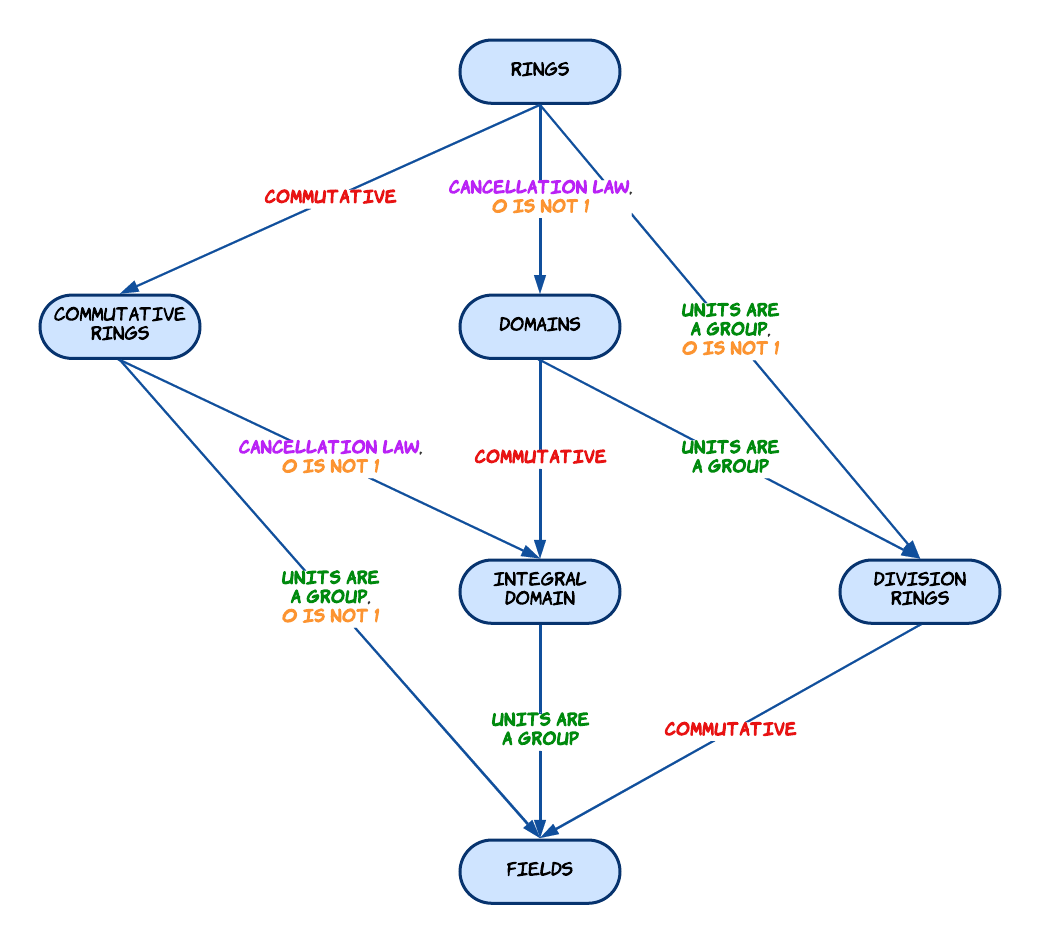
\includegraphics[scale = 0.3]{Ring Diagram}
\centering
\end{figure}

I like that there is a subtle sense of symmetry here. The conditions on the arrow is the condition for the ring in the tail to be a ring in the arrow head. For instance, if a domain $R$ satisfies the property that elements in $R$ are commutative, then $R$ is an integral domain. On the other hand, every integral domain will necessarily be a domain. 

\pagebreak
\subsection{Ring Homomorphisms and Ideals}
\begin{defn}{Ring Homomorphism}{} Let $R,S$ be rings. A ring homomorphism is a map $\phi:R\to S$ such that $$\phi(a+b)=\phi(a)+\phi(b)$$ and $$\phi(ab)=\phi(a)\phi(b)$$ for all $a,b\in R$. A bijective ring homomorphism is called a ring isomomorphism. 
\end{defn}

\begin{defn}{Kernel}{} The kernel of the ring homomorphism $\phi$, denoted $\ker(\phi)$ is defined as $$\ker(\phi)=\{r\in R|\phi(r)=0\}$$
\end{defn}

\begin{defn}{Ideals}{} Let $R$ be a ring. Let $I\subset R$ and let $r\in R$. Define $rI=\{ra|a\in I\}$ and $Ir=\{ar|a\in I\}$
\begin{itemize}
\item $I$ is a left ideal of $R$ if $(I,+)$ is a subgroup of $(R,+)$ and $rI\subseteq I$ for all $r\in R$
\item $I$ is a right ideal of $R$ if $(I,+)$ is a subgroup of $(R,+)$ and $Ir\subseteq I$ for all $r\in R$
\item A subset $I$ that is both a left ideal and right ideal is called an ideal of $R$. 
\end{itemize}
\end{defn}

\begin{lmm}{}{} Let $I$ be an ideal of a ring $R$. Then $I=R$ if and only if there exists a unit $u\in R$ such that $u\in I$. \tcbline
\begin{proof}
Let $I=R$. Then trivially $u\in I$. Now let $u\in I$ be a unit. Let $x\in R$, I want to show that $x\in I$ thus completing the proof that $R\subseteq I$. Now $x=x(u^{-1}u)=(xu^{-1})u$. Since $xu^{-1}\in R$ and $u\in I$, their muplication will also be in $I$, thus $x\in I$. 
\end{proof}
\end{lmm}

This lemma is also very useful if you consider the fact that the mupltiplicative identity is also a unit. 

\begin{prp}{}{} If $I,J$ are ideals of a ring $R$ then $$I+J=\{i+j|i\in I,j\in J\}$$ and $$I\cap J=\{r\in R|r\in I,r\in J\}$$ are both ideals of $R$. \tcbline
\begin{proof}
Let $R$ be a ring and $I,J$ its ideals. 
\begin{itemize}
\item We first show that $I+J$ is an ideal. Let $i_1+j_1,i_2+j_2\in I+J$. Then since $R$ is an abelian group an $I,J$ are subgroups of $R$, $$i_1+j_1+i_2+j_2=(i_1+i_2)+(j_1+j_2)\in I+J$$ thus closure is satisfied. Associativity is satisfied since it inherits from $R$. We also have $0\in I,J$ thus $0\in I+J$. The inverse of $i+j\in I+J$ is $-i-j\in I+J$ since $-i\in I$ and $-j\in J$. Thus $I+J$ is a subgroup of $R$. \\~\\
Now let $r\in R$ and $i+j\in I+J$. Then $r(i+j)=ri+rj$ by distributivity. Since $I,J$ are ideals, there exists $s\in I$ such that $s=ri$ and $t\in J$ such that $t=rj$. Then $r(i+j)=ri+rj=s+t\in I+J$ thus we are done. 
\item $I\cap J$ are already subgroups of $R$. Let $k\in I\cap J$. Let $r\in R$. Then $rk\in r(I\cap J)$. Then there exists $i\in I$ and $j\in J$ such that $i=rk=j$. Then $i=j\in I\cap J$ thus we are done. 
\end{itemize}
\end{proof}
\end{prp}

\begin{prp}{}{} The kernel of any ring homomorphism is an ideal. \tcbline
\begin{proof}
Kernels are trivially subgroups of $(R,+)$. Let $r\in R$. Let $x\in\ker(\phi)$. Then $\phi(rx)=\phi(r)\phi(x)=\phi(r)\cdot 0\in\ker(\phi)$ thus we are done. 
\end{proof}
\end{prp}

\begin{prp}{Quotient Ring}{} Let $I$ be an ideal of a ring $R$. Then the cosets of $I$ in $R$, $$R/I=\{r+I|r\in R\}$$ is a ring with addition defined the same as quotient groups $$(r+I)+(s+I)=(r+s)+I$$ and multiplication defined as $$(r+I)(s+I)=\{ab\in R|a\in r+I,b\in s+I\}=rs+I$$ called the quotient ring of $R$ by $I$. \tcbline
\begin{proof}
Since $(I,+)$ is a subgroup of $(R,+)$, we know that $R/I$ is already an abelian group. We simply show that multplication is well defined. Suppose that $x_1+I=x_2+I$ and $y_1+I=y_2+I$. Then 
\begin{align*}
(x_1+I)(y_1+I)&=x_1y_1+I\\
&=(x_1y_1-x_1y_2+x_1y_2-x_2y_2+x_2y_2)+I\\
&=(x_1(y_1-y_2)+(x_1-x_2)y_2+x_2y_2)+I\\
&=x_2y_2+I
\end{align*}
since $y_1-y_2\in I$ and $x_1-x_2\in I$. This shows that taking different represetatives of the cosets of an ideal does not matter for multiplication. \\~\\
Now we show that $1+I$ is the muplicative identity of $R/I$. Let $x+I\in R/I$. We have that $(1+I)(x+I)=x+I$ thus we are done. Associativity and distributivity follows from the fact that $R$ has these properties. 
\end{proof}
\end{prp}

\begin{thm}{}{} If $I$ is an ideal of $R$, the map $\phi:R\to R/I$ defined by $\phi(r)=r+I$ is a surjective ring homomorphism with kernel $I$. \tcbline
\begin{proof}
Let $a,b\in R$. Then 
\begin{align*}
\phi(a+b)&=(a+b)+I\\
&=(a+I)+(b+I)\\
&=\phi(a)+\phi(b)
\end{align*}
Now let $r\in R$. Then
\begin{align*}
\phi(ra)&=ra+I\\
&=(r+I)(a+I)\\
&=\phi(r)\phi(a)
\end{align*}
Now we show that $\phi$ is surjective. Let $r+I\in R/I$. Then trivially $\phi(r)=r+I$ thus we are done. \\~\\
Finally we show that $\ker(\phi)=I$. Let $a\in\ker(\phi)$. Then $\phi(a)=a+I=I$. This means that $a\in I$ and we have shown that $\ker(\phi)\subseteq I$. Now suppose that $a\in I$. Then $\phi(a)=a+I=I$. Thus $a\in\ker(\phi)$ and we are done. 
\end{proof}
\end{thm}

\subsection{Types of Ideals}
\begin{lmm}{}{} Let $R$ be a commutative ring and $a\in R$. Then $(a)=\{ar:r\in R\}$ is an ideal. \tcbline
\begin{proof}
Let $s,t\in(a)$. Then $s=ar_1$ and $t=ar_2$ for some $r_1,r_2\in R$. We show that $(a)$ is a subgroup of $R$. We have $$s+t=a(r_1+r_2)\in(a)$$ Identity is also in $(a)$ since $0\in R$ and $$a\cdot 0=0\in(a)$$ To show inverse we have that $u=-ar_1$ and $$s+u=ar_1-ar_1=0$$ By the subgroup criterion, $(a)$ is a group. We now show that $r(a)\subseteq(a)$. Let $r_1ar_2\in r(a)$. Then $$r_1ar_2=ar_1r_2\in(a)$$ since $R$ is commutative. Thus $(a)$ is an ideal. 
\end{proof}
\end{lmm}

\begin{defn}{Principal Ideals}{} Let $R$ be a commutative ring with identity. Let $I$ be an ideal of $R$. Then an ideal $I$ of the form $$I=(a)$$ for some $a\in I$ is called a principal ideal. 
\end{defn}

\begin{defn}{Maximal Ideals}{} A proper ideal $M$ of a ring $R$ is a maximal ideal of $R$ is the ideal $M$ is not a proper subset of any ideal of $R$ except $R$ itself. 
\end{defn}

Becareful that maximal ideals are not necessarily unique. A typical example would be the fact that $(2)$ and $(3)$ are principle ideals that are both maximal in $\Z$. 

\begin{defn}{Prime Ideals}{} A proper ideal $P$ in a commutative ring $R$ is called a prime ideal if $ab\in P$ implies $a\in P$ or $b\in P$. 
\end{defn}

\begin{prp}{}{} Let $R$ be a commutative ring with identity and $M$ an ideal of $R$. Then $M$ is maximal if and only if $R/M$ is a field. \tcbline
\begin{proof}
Suppose that $M$ is a maximal ideal. Let $x\notin R$. We show that $x+M$ has an inverse. We know that $M+(x)$ is an ideal containing $M$. Since $M$ is maximal, we must have $M+(x)=R$. This means that $1\in M+(x)$ which means there exists $m\in M$ and $r\in R$ such that $1=m+rx$. Now consider $r+M$. We have that 
\begin{align*}
(x+M)(r+M)&=xr+M\\
&=(1-m)+M\\
&=1+M
\end{align*}~\\
Now suppose that $R/M$ is a field. Let $J$ be an ideal such that $I\subseteq J\subseteq R$ and $I\neq J$. Now let $x\in J\setminus I$. Then $I+x$ has a multiplicative inverse in $R/I$ since $I+x\neq I$, the additive identity. Let the inverse be $I+y$. Then $$I+1=(I+x)(I+y)=I+xy$$ Trivially $xy\in(x)$, thus $1\in I+(x)\subseteq J$. But if the identity is in the ideal, the ideal is equal to the ring thus we are done. 
\end{proof}
\end{prp}

\begin{prp}{}{} Let $R$ be a commutative ring with identity not equal to $0$. Then $P$ is a prime ideal in $R$ if and only if $R/P$ is an integral domain. \tcbline
\begin{proof}
Suppose that $P$ is a prime ideal. Then let $(a+P)(b+P)=P$. Since we also have that $(a+P)(b+P)=ab+P$. This means that $ab\in P$ thus either $a\in P$ or $b\in P$ which in turns leads to either $a+P=P$ or $b+P=P$ and thus the cancellation law applies. \\~\\
Now suppose that $R/P$ is an integral domain. Let $ab\in P$. Since $R/P$ is an integral domain, we have that $$(a+P)(b+P)=ab+P=P$$ means that either $a+P=P$ or $b+P=P$ which means that either $a\in P$ or $b\in P$ and we are done. 
\end{proof}
\end{prp}

\begin{crl}{}{} Every maximal ideal in a commutative ring with identity is also a prime ideal. \tcbline
\begin{proof}
If $M$ is maximal then $R/M$ being a field implies that $R/M$ is an integral domain thus $M$ is prime. 
\end{proof}
\end{crl}

The proof is rather inconstructive in the sense that it does not provide a good insight to the structure, the reasoning behind why every maximal ideal is prime. For a more structure-revealing proof, consider the following alternative approach: \\~\\
Let $M$ be a maximal ideal of a commutative ring $R$. Let $ab\in M$ but $a\notin M$. Then $M+(a)=R$ since $M$ is maximal. Then $1\in R$ means that there exists $k\in M$ and $r\in R$ such that $k+ra=1$. Mutplying by $b$ gives $kb+rab=b$. Since $kb\in M$ and $rab\in M$, $b\in M$ and we are done. 

\pagebreak
\section{Integral Domains}
\subsection{Field of Fractions}
\begin{defn}{Fractional Equivalence}{} Let $R$ be an integral domain. Let $$S=\{(a,b)|a,b\in R\text{ and }b\neq 0\}$$ Define a relation on $S$ by $(a,b)\sim(c,d)$ if $ad=bc$. 
\end{defn}

\begin{lmm}{}{} The relation $\sim$ between elements of $S$ is an equivalence relation. \tcbline
\begin{proof}
Since $R$ is an integral domain, symmetry is satisfied. Clearly it is reflexive since $ab=ba$. For transitivity, suppose that $ad=bc$ and $cf=de$. Then $adcf=bcde$ and by cancellation law, $af=be$. 
\end{proof}
\end{lmm}

\begin{prp}{}{} The set of equivalence classes of $S$ of an integral domain $R$, under the equivalence relation $\sim$, together with the operations of addition and multiplication defined by $$(a,b)+(c,d)=(ad+bc,bd)$$ and $$(a,b)\cdot(c,d)=(ac,bd)$$ is a field, called the field of fractions, denoted $\text{Frac}(R)$. \tcbline
\begin{proof} Note that $R$ is a field if and only if $(R,+)$ and $(R\setminus\{0\},\cdot)$ are commutative groups and the distributive law holds. 
\begin{itemize}
\item Let $(a,b),(c,d)\in S$. Then $ad+bc,bd\in R$ since $R$ is closed thus $(ad+bc,bd)\in S$. Let $(e,f)$ also be in $S$. Then 
\begin{align*}
((a,b)+(c,d))+(e,f)&=(ad+bc,bd)+(e,f)\\
&=((ad+bc)f+(bd)e,bdf)\\
&=(adf+bcf+bde,bdf)
\end{align*}
and 
\begin{align*}
(a,b)+((c,d)+(e,f))&=(a,b)+(cf+de,df)\\
&=(a(df)+b(cf+de),b(df))\\
&=(adf+bcf+bde,bdf)
\end{align*}
Thus associativity is satisfied. I claim that $(0,1)$ is an identity. We have $(a,b)+(0,1)(a\cdot 1+b\cdot 0,b\cdot 1)=(a,b)$. If $(a,b)\in S$ then $(-a,b)\sim(a,-b)$ is an inverse. We have $$(a,b)+(-a,b)=(ab-ab,b^2)=(0,b^2)\sim(0,1)$$ Finally we have 
\begin{align*}
(a,b)+(c,d)&=(ad+bc,bd)\\
&=(da+cb,db)\tag{$R$ is an Integral Domain}\\
&=(cb+da,db)\tag{$R$ is an abelian group}
&=(c,d)+(a,b)
\end{align*}
Thus we have shown that $(S,+)$ is an abelian group. 
\item We now show that $(S,\cdot)$ is an abelian group. Let $(a,b),(c,d),(e,f)\in S$. Then $(a,b)\cdot(c,d)=(ac,bd)\in S$ sincve $ac,bd\in R$ by closure of rings. Thus the closure property is satisfied. Associativity is inherited from $R$ since elements in $S$ are pairs of $R$. I claim that the identity is $(1,1)\sim(k,k)$ for any $k\in R$. We have $$(a,b)\cdot(1,1)=(a\cdot1,b\cdot 1)=(a,b)$$ If $(a,b)\in S$ then its inverse is $(b,a)$. We have $$(a,b)\cdot(b,a)=(ab,ba)=(ab,ab)=(1,1)$$ thus $(S,\cdot)$ is a group. Now to show abelian, we have $$(a,b)\cdot(c,d)=(ac,bd)=(ca,db)=(c,d)\cdot(a,b)$$ since $R$ is an integral domain. Thus we have shown that $(S,\cdot)$ is an abelian group. 
\item Finally we show distributivity. Let $(a,b),(c,d),(e,f)\in S$. Then 
\begin{align*}
(a,b)\cdot((c,d)+(e,f))&=(a,b)\cdot(cf+de,df)\\
&=(acf+ade,bdf)
\end{align*}
and 
\begin{align*}
(a,b)\cdot(c,d)+(a,b)\cdot(e,f)&=(ac,bd)+(ae,bf)\\
&=(acbf+bdae,bdbf)\\
&=(acf+ade,bdf)\tag{equivalence relation}
\end{align*}
Thus we are done. 
\end{itemize}
\end{proof}
\end{prp}

In particular, the field of fractions of $\Z$ is precisely $\Q$. 

\begin{lmm}{}{} For any integral domain $R$, $R$ is a subring of $\text{Frac}(R)$. \tcbline
\begin{proof}
Define a function $\phi:R\to Q(R)$ by $\phi(r)=\frac{r}{1}$. Then $\phi_R$ is the identity homorphism thus $\phi(R)=R$. Then $\phi(R)$ is trivially a subring of $Q(R)$ and we are done. 
\end{proof}
\end{lmm}

\subsection{Divisibility}
\begin{defn}{Division}{} Let $R$ be a commutative ring and let $a,b\in R$ with $b\neq 0$. $a$ is said to be a multiple of $b$ if there exists an element $x\in R$ with $a=bx$. In this case $b$ is said to divide $a$ or be a divisor of $a$, written $b|a$. 
\end{defn}

\begin{prp}{}{} Let $R$ be a commutative ring. Let $x,y\in R$ and $y\neq 0$. Then the following are equivalent. 
\begin{itemize}
\item $x|y$
\item $y\in(x)$
\item $(y)\subseteq(x)$
\end{itemize}\tcbline
\begin{proof} Let $R$ be a commutative ring. Let $x,y\in R$ and $y\neq 0$. 
\begin{itemize}
\item $(1)\implies(2)$ Suppose that $y=kx=xk$ for some $k\in R$. Then $y\in(x)=\{ax|a\in R\}$ by definition. 
\item $(2)\implies(3)$ Suppose that $y\in(x)$. Then there exists $k\in R$ such that $y=kx=xk$. To show that $(y)\subseteq(x)$, let $ry\in(y)$. Then $ry=rkx$ and $rk\in R$ thus $ry\in(x)$ thus we are done. 
\item $(3)\implies(1)$ Suppose that $(y)\subseteq(x)$. Then there exists $k\in R$ such that $y=kx$. Then we are done. 
\end{itemize}
\end{proof}
\end{prp}

\begin{defn}{Greatest Common Divisor}{} A greatest common divisor of $a$ and $b$ is a non-zero element $d$ such that 
\begin{itemize}
\item $d|a$ and $d|b$
\item If $c|a$ and $c|b$ then $c|d$
\end{itemize} It is denoted $\gcd(a,b)$. 
\end{defn}

\begin{defn}{Least Common Multiple}{} A least common multiple of $a$ and $b$ is a non-zero element $l$ such that 
\begin{itemize}
\item $a|l$ and $b|l$
\item If $a|m$ and $b|m$ then $l|m$
\end{itemize} It is denoted $\lcm(a,b)$. 
\end{defn}

Unfortunately, these numbers do not always exists for any $a,b$ in a general ring. We will prove their existence in principal ideal domains later. 

\begin{prp}{}{} Let $R$ be a commutative ring. Let $x,y\in R$ such that they are nonzero. If the ideal generated by $a$ and $b$, namely $(a,b)$ is a principal ideal $(d)$, then $d$ is the gcd of $a$ and $b$. \tcbline
\begin{proof}
Suppose that $(a,b)=(d)$ for some $d\in R$. Then $a\in(d)$ and $b\in(d)$ already implies that $d|a$ and $d|b$. Suppose that $c|a$ and $c|b$. This means that $a\in(c)$ and $b\in(c)$. Since $d\in(a,b)$ there exists $r,s\in R$ such that $ra+sb=d$. This means that $d\in(c)$ thus $c|d$. 
\end{proof}
\end{prp}

This explains the notation that $(a,b)$ is often used to denote the gcd. 

\begin{defn}{Associates}{} Let $R$ be a commutative ring. Let $x,y\in R$. We say that $x$ and $y$ are associates if $x|y$ and $y|x$. We denote it as $x\sim y$. 
\end{defn}

\begin{prp}{}{} Let $R$ be a integral domain. Let $x,y\in R$. Then the following are equivalent. 
\begin{itemize}
\item $x\sim y$
\item $(x)=(y)$
\item There exists a unit $u\in R$ such that $x=qy$. 
\end{itemize} \tcbline
\begin{proof}
\begin{itemize}
\item $(1)\implies(2)$: Suppose that $x\sim y$ then $x|y$ and $y|x$ which means that $(x)\subseteq(y)$ and $(y)\subseteq(x)$. 
\item $(2)\implies(3)$: Suppose that $(x)=(y)$. Then since $x\in(y)$, there exists $s\in R$ such that $x=sy$ and likewise $y=tx$. Then $x=stx$ and since $R$ is an integral domain, $st=1$ which means that $s,t$ are units. 
\item $(3)\implies(1)$: Suppose that $x=qy$ for some unit $q$. Then clearly $y|x$. Since $q$ is a unit, $q^{-1}x=y$ and thus $x|y$ which means that $x$ and $y$ are associates. 
\end{itemize}
\end{proof}
\end{prp}

\subsection{Primes and Irreducibles}
Primes and irreducibles are two similar concepts, their difference is only made clear in Euclidean domains that are not principles ideal domains which we will see both notions later. 

\begin{defn}{Irreducibles}{} Let $D$ be an integral domain. A nonzero element $p\in D$ that is not a unit is said to be irreducible if $p=ab$ implies $a$ or $b$ is a unit. 
\end{defn}

\begin{defn}{Primes}{} Let $D$ be an integral domain. A nonzero element $p\in D$ that is not a unit is said to be a prime if $p|ab$ implies $p|a$ or $p|b$. 
\end{defn}

\begin{lmm}{}{} Let $D$ be an integral domain. Let $p$ be a non-unit. Then $p$ is prime if and only if $(p)$ is a prime ideal. \tcbline
\begin{proof}
Suppose that $p$ is prime. Suppose that $rp\in(p)$. Then $p\in P$ and we are done. Now suppose that $(p)$ is a prime ideal. Suppose that $p|ab$. Then $pd=ab$ for some $d\in D$ thus $ab\in(p)$. WLOG take $a\in(p)$ by definition of prime ideal. Then we are done since $a\in(p)$ implies $p|a$. 
\end{proof}
\end{lmm}

\begin{prp}{}{} Let $D$ be an integral domain and $p\in D$. If $p$ is a prime then $p$ is irreducible. \tcbline
\begin{proof}
Let $p$ be a prime in $D$. Suppose that $p=ab$. Then trivially $p|ab$ thus $p|a$ or $p|b$. WLOG take $p|a$. Trivially $a|p$ since $a|ab$. This means that $a$ and $p$ are associates. Thus $p=aq$ for some unit $q$. Then since $aq=ab$ and integral domains have cancellation law, we must have $q=b$ which means that $b$ is a unit. Thus $p$ is irreducible. 
\end{proof}
\end{prp}

\subsection{Unique Factorization Domains}
\begin{defn}{Unique Factorization Domains}{} An integral domain $D$ is a unique factorization domain if the following are true
\begin{itemize}
\item Let $a\in D$ such that $a\neq 0$ and $a$ is not a unit. Then $a$ can be written as the product of irreducible elements in $D$. 
\item Let $a=p_1\cdots p_r=q_1\cdots q_s$, where $p_i$ and $q_j$ are irreducible. Then $r=s$ and there is a permutation such that $p_i=q_{\pi(i)}$ for $i\in\{1,\dots,r\}$. 
\end{itemize}
\end{defn}

Notice that in general integral domains, primes are not the same as irreducibles. But they have the nice property that they coincide in UFDs, which is why they are put in the chapter on UFDs here. Below gives a full converse to the relation between prime and irreducibles we gave above under the umbrealla that is UFDs. 

\begin{prp}{}{} Let $D$ be a UFD and $p\in D$. Then $p$ is a prime if and only if $p$ is irreducible. \tcbline
\begin{proof}
We have already shown the forward implication. Now let $p$ be irreducible. We show that $(p)$ is prime. Let $ab\in(p)$. Then there exists $d\in D$ such that $pd=ab$. We can factorize $ab$ and $pd$ respectively into a product of irreducibles elements in $D$. But since they are equal, by uniqness of fatorization, $p$ is exactly an associate of one of the irreducibles in the factorization of $ab$. If $p$ is in the factorization of $a$ then $p|a$ and we are done. Otherwise it is in $b$ and we are also done. 
\end{proof}
\end{prp}

Notice that in the above proof, the fact that every prime is irreducible does not use the properties of UFD. This means that this is true in general integral domains. 

\subsection{Principal Ideal Domains}
\begin{defn}{Principal Ideal Domains}{} A principal ideal domain is an integral domain in which every ideal is principal, meaning every ideal is of the form $$(a)=\{ra:r\in R\}$$
\end{defn}

\begin{prp}{}{} Let $R$ be a PID and $x,y\in R$. Then $\gcd(x,y)$ and $\lcm(x,y)$ exists and there exists $r,s\in R$ such that $$\gcd(x,y)=rx+sy$$ \tcbline
\begin{proof}
Let $x,y\in R$. Then $(x)+(y)$ is an ideal of $R$, thus it must be prciniple, say $(d)=(x)+(y)$. Similarly, $(x)\cap(y)$ is also an ideal, say $(l)=(x)\cap(y)$. \\~\\
We prove that $d$ and $l$ are the gcd and lcm respectively. Trivially, $(x)\subseteq(d)$ and $(y)\subseteq(d)$ implies $d|x$ and $d|y$. Also for any $z$ such that $z$ divides $x$ and $y$, $(x)\subseteq(z)$ and $(y)\subseteq(z)$ thus $(d)\subseteq(z)$. The proof is similar for $(l)$. \\~\\
Since $(d)=(x)+(y)$, there exists $r,s\in (x),(y)$ respectively such that $d=rx+sy$ and we are done. 
\end{proof}
\end{prp}

\begin{prp}{}{} Let $R$ be a PID and $(p)$ a nonzero ideal in $R$. Then the following are equivalent. 
\begin{itemize}
\item $(p)$ is maximal
\item $p$ is irreducible
\item $p$ is prime ($(p)$ is prime)
\end{itemize} \tcbline
We have seen that every maximal ideal is a prime ideal. We have seen that if $(p)$ is a prime ideal then $p$ is prime. We have also seen that every prime is irreducible. We show separately that if $p$ is irreducible then $p$ is a prime, and also if $p$ is prime then $(p)$ is maximal. \\~\\
For the first part, suppose that $p$ is irreducible. Suppose that $p|ab$ for $a,b\in R$. By the above proposition, $d=\gcd(p,a)$ exists. Then for some $t\in R$, $p=dt$. Since $p$ is irreducible, either $d$ or $t$ is a unit. We consider both cases. If $t$ is a unit, then $p$ and $d$ are associates and thus $p|d$. Since $d|a$, we have that $p|a$ and we are done. Now if $d$ is a unit, then $d=ra+sp$ for some $r,s\in R$. Multplying both sides with $b$ gives $db=rab+spb$. Since $p|ab$ and $p|spb$, we have that $p|db$. Then $pu=db$ for some unit $u\in R$. Since $d$ is a unit, we have that $d^{-1}pu=b$, which means that $p|b$ and we are done. \\~\\
Now we show that if $p$ is a prime then $(p)$ is maximal. We know that $(p)$ is a prime ideal. Suppose that $(p)\subseteq(q)\subseteq R$ for some ideal $q$ of $R$. Since $p\in(q)$, $p=tq$ for some $t\in R$. Since $p\in(p)$, we have that $tq\in(p)$. Now $(p)$ is prime implies that either $t\in(p)$ or $q\in(p)$. If $q\in(p)$ then $(q)\subseteq(p)$ and thus $(q)=(p)$ and we are done. If $t\in(p)$, then $t=rp$ for some $r\in R$, which means that $p=rpq$. Then $rq=1$ by cancallation law in integral domains. This means that $1\in(q)$ thus $(q)=R$ and we are done. 
\end{prp}

\begin{prp}{}{} Every PID is a UFD. \tcbline
\begin{proof}
Suppose that $D$ is a principal ideal domain. Suppose for a contradiction that $x$, a non-unit cannot be factorized into a product of irreducibles. Clearly $x$ is not irreducible else a contradiction. Then there exists $x_1,y_1$ non unit such that $x=x_1y_1$. Since $x$ is assumed to be not a product of irreducibles, WLOG take $x_1$ to be not irreducible. Then we can repeat the process to get non units $x_2y_2$ such that $x_1=x_2y_2$. Notice that $(x)\subset(x_1)$ is a proper containment of ideals if $x_1|x$. Then we have a chain of ideals $$(x)\subset(x_1)\subset(x_2)\subset\dots$$ I claim that $$I=\bigcup_{k=0}^\infty(x_k)$$ is an ideal. Indeed if $r,s\in I$, then $r\in(x_m)$ and $s\in(x_n)$ for some $m,n\in\N$. WLOG rtake $m\leq n$. Then $(x_m)\subseteq(x_n)$ implies $r,s\in(x_n)$ thus $r+s\in(x_n)\subseteq I$. Also if $t\in R$, then $tr\in(x_m)\subseteq I$ thus $I$ is indeed an ideal. \\~\\
Since $R$ is a PID, there exists some $d\in I$ such that $I=(d)$. This also means that $d\in(x_m)$ for some $m\in\N$. Then this means that $I=(d)\subseteq(x_m)$. This proves that the chain eventually stops and this is a contradiction since we assumed that the chain of ideals are properly contained. \\~\\
This menas that $x$ can indeed be factorized into a product of irreducibles. 
\end{proof}
\end{prp}

Notice that the key in the proof is that the union of the countably finite principal ideals is again a principal ideals which allows the infinte chain of ideals to stop. 

\subsection{Euclidean Domains}
Technically, division algorithms can exist in general domains so long that it has the notion of division. But without a measurement of size to guarantee division is taking larger numbers into smaller numbers, we cannot promise that division algorithms will halt eventually. Therefore we restrict the notion of division algorithm only to integral domains that has a notion of size. 
\begin{defn}{Euclidean Valuation}{} Let $R$ be an integral domain. A function $f:R\setminus\{0\}\to\N\cup\{0\}$ is said to be a Euclidean Valuation of $R$ if
\begin{itemize}
\item $f(ab)\geq f(b)$ for all $a,b\in R\setminus\{0\}$
\item For all $a,b\in R$ with $b\neq0$, there exists $q,r$ such that $$a=qb+r$$ with $r=0$ or $f(r)<f(b)$
\end{itemize}
\end{defn}

In the above definition the second item is simply the division algorithm, with size of a number decided by the function $f$. Thus the Euclidean domain is simply an integral domain that possess a division algorithm. 

\begin{defn}{Euclidean Domain}{} An integral domain $R$ is said to be a Euclidean Domain that admits a Euclidean Valuation
\end{defn}

\begin{thm}{}{} Let $R$ be a Euclidean Domain. Let $a,b$ be nonzero elements of $R$. Let $d=r_n$ be the last nonzero remainder in the Euclidean Algorithm for $a$ and $b$. Then $d$ is the greatest common divisor of $a$ and $b$ and $(d)$ is generated by $a$ and $b$. In particular, there exists $x,y\in R$ such that $d=ax+by$. 
\end{thm}

\begin{prp}{}{} Every Euclidean Domain is a PID. 
\end{prp}

In general, we have that $$\text{Fields}\subset\text{Euclidean Domains}\subset\text{PID}\subset\text{UFD}\subset\text{Integral Domains}$$ in which all containments are strict. 

\pagebreak
\section{Polynomials}
\subsection{Polynomials over General Rings}
In this section we formulate the basic theory of generating polynomials from a ring. 
\begin{defn}{Indeterminates}{} Let $R$ be a ring. A symbol $x$ is called an indeterminate over $R$ if $$a_0+a_1x+a_2x^2+\dots+a_nx^n=0$$ where $a_i\in R$, implies that $a_i=0$ for each $i$. 
\end{defn}

\begin{defn}{Polynomial over a Ring}{} Any expression of the form $$f(x)=\sum_{k=0}^na_kx^k$$ where $x$ is an indeterminate and $a_0,\dots,a_n\in R$ and $a_n\neq 0$ is called a polynomial over $R$. We define the the degree of $f$ in this case to be $n$. 
\end{defn}

\begin{defn}{Ring of Polynomials}{} Let $R$ a ring. Define $R[x]$ to be the set of all polynomials over $R$. 
\end{defn}

\begin{prp}{}{} Let $R$ be a commutative ring with identity. Then $R[x]$ is a commutative ring with identity. \tcbline
\begin{proof}
Since $R\leq R[x]$ by considering all the constant polynomials, the identity of $R$ is also the identity of $R[x]$. Let $f,g\in R[x]$. Then the coefficient of $x^n$ in $f(x)g(x)$ is $$c_n=\sum_{k=0}^na_kb_{n-k}$$ Since $a_kb_{n-k}=b_{n-k}a_k$, we have that $f(x)g(x)=g(x)f(x)$. 
\end{proof}
\end{prp}

\begin{lmm}{}{} Let $R$ be a ring. Then $$\frac{R[x]}{(x)}\cong R$$ \tcbline
\begin{proof}
Taking the natural homomorphism $\phi:R[x]\to\frac{R[x]}{(x)}$ where $(x)$ is the ideal, we have that $\ker(\phi)=(x)$. By the first ring isomorphism theorem, $$\frac{R[x]}{(x)}\cong\phi(R[x])$$ But $\phi(R[x])$ is isomorphic to $R$ since every polynomial in $R[x]$ is a sum of a constant function and an element in $(x)$. 
\end{proof}
\end{lmm}

Whenever something similar to the above notion is seen, say $\frac{\Q[x]}{x-3}$, one can think of it as, whenever I see a factor of $x-3$ in $\Q[x]$, treat it as $0$. So if you want to find the image of $x^2-4x+5$ in the ring, we simply see that $x^2-4x+5=(x-3)(x-1)+2=2$ since $x-3$ is treated as $0$. Recalling that this is the quotient ring, we essentially quotient out all polynomials that has this factor which leads to $x^2-4x+5$ being treated as the same as the element $2$ in the ring. 

\begin{thm}{Evaluation Theorem}{} Let $R$ be a ring and let $a$ be an element in the center $Z(R)$ of $R$. Define a mapping $\phi_a:R[x]\to R$ by $$\phi_a\left(\sum_{k=0}^nc_kx^k\right)=\sum_{k=0}^nc_ka^k$$ Then $\phi_a$ is an onto ring homomorphism. 
\end{thm}

The evaluation maps gives a useful ring homomorphism to construct quotient rings. 

\subsection{Polynomials over Integral Domains}
\begin{prp}{}{} If $R$ is an integral domain then $R[x]$ is an integral domain. In particular the units in $R$ are also units in $R[x]$. \tcbline
\begin{proof}
Commutativity is clear since for $f,g\in R[x]$, coefficients of the product $fg$ inherits commutativity from $R$ thus $fg=gf$. Now we show that cancellation law exists in $R[X]$. Let $f,g\in R[x]$ such that $fg=0$. Suppose for a contradiction that $f\neq 0$ and $g\neq 0$. This means that $\deg(f)=n$ and $\deg(g)=m$ for some $n,m\neq 0$. Consider the coefficient of $x^{n+m}$ in $fg$, which is $a_nb_m$. Since $fg=0$, $a_nb_m=0$ and by cancellation law in $R$ either $a_n=0$ or $b_m=0$. This contradicts the fact that $\deg(f)=n$ and $\deg(g)=m$ thus we are done. \\~\\
The second part is trivial since $R\leq R[x]$ and they have the same identity. 
\end{proof}
\end{prp}

\begin{prp}{}{} Let $R$ be an integral domain. Then if $f\neq 0$ and $g\neq 0$ in $R[x]$, then $$\deg(fg)=\deg(f)+\deg(g)$$
\end{prp}

\begin{defn}{Irreducible Polynomial}{} Let $F$ be a field. A non constant polynomial $f\in F[x]$ is irreducible over $F$ if whenever $f(x)=g(x)h(x)$ with $g,h\in F[x]$, then one of $g$ or $h$ is a unit. 
\end{defn}

This defintion corresponds to the same definition of irreduciblesgiven in the UFD section. 

\subsection{Polynomials over UFDs}
The primary goal of this chapter is to compute results relating to finding out ireducible polynomials in UFD, rather than investigating the structure of polynomial rings. 
\begin{defn}{Primitive}{} An element $0\neq f\in R[x]$ where $R$ is a unique factorization domain is called primitive if $\gcd(a_0,a_1,\dots,a_n)=1$. 
\end{defn}

The reason that we have this notion is to prevent polynomials such as $5x-5$ to be discussed. This clearly will not be irreducible since there is a factor of $5$. Likewise if the gcd of all its coefficients are not $1$, then you can factor out the gcd from the entire polynomial. 

\begin{prp}{}{} The productive of two primitive polynomials is also primitive. 
\end{prp}

\begin{prp}{Eisentein's Criterion}{} Let $R$ be a UFD. Let $f\in R[x]$ be primitive. Suppose there is a prime $p\in R$ such that $p$ does not divide $a_n$ but $p|a_i$ for $0\leq i\leq n-1$ and $p^2$ does not divide $a_0$. Then $f$ is irreducible in $R[x]$. 
\end{prp}

\begin{thm}{}{} Let $R$ be a UFD with field of fractions $Q=Q(R)$. Then a primitive polynomial in $R[x]$ is irreducible if and only if it is irreducible in $Q[x]$. 
\end{thm}

An immediate corollary for when $R=\Z$ is as follows. 

\begin{thm}{Gauss' Lemma}{} A primitive irreducible polynomial in $\Z[x]$ remains irreducible in $\Q[x]$
\end{thm}

\begin{prp}{}{} $R$ is an UFD if and only if $R[x]$ is an UFD. 
\end{prp}

\subsection{Polynomials over a Field}
This section will mainly be revisiting old notations with $F[x]$. 
\begin{thm}{Division Algorithm}{} Let $F$ be any field and let $f$ and $g$ be polynomials in $F[x]$. Assume that $f\neq0$ and that the leading coefficient of $f$ is a unit in $R$. Then uniquely determined polynomials $q$ and $r$ exist in $F[x]$ such that 
\begin{itemize}
\item $g=qf+r$
\item Either $r=0$ or $\deg(r)<\deg(f)$
\end{itemize}
In particular, $\deg$ is an Euclidean Valuation of $F[x]$ and $F[x]$ is a Euclidean domain. 
\end{thm}

The above theorem is equivalent to saying that $F[x]$ is a Euclidean domain as long as $F$ is a field. Trivially, this also means that $F[x]$ is both a principal ideal domain and a unique factorization domain. \\~\\
We give an alternate proof showing that $F[x]$ is a principal ideal domain. \\~\\
Let $I$ be a nontrivial ideal of $F[x]$. Let $f\in I$ be nonzero such that the degree of $f$ is as small as possible. I claim that $(f)=I$. We already have that $(f)\subseteq I$ since $f\in I$. Now we show that $I\subseteq(f)$. So let $g\in I$. By the division algorithm, write $g=fq+r$ for some $q,r$ such that $\deg(r)<\deg(f)$ or $\deg(r)=0$. If $r\neq 0$, then $r=g-fq\in I$ since $f,g\in I$. But then $\deg(r)<\deg(f)$ means that $f$ is not of smallest degree in $I$, a contradiction. Thus $g=fq$, which means that $g\in(f)$. \\~\\
This is a constructive proof in the sense that if we would like to know the sole generator of an ideal in a polynomial ring $F[x]$ of a field, we simply take the polynomial of lowest degree. \\~\\

Since we have shown that polynomials over a field are euclidean domains, the following theorems and definitions are also trivial. 

\begin{lmm}{}{} Let $F$ be a field and suppose that $p\in F[x]$. Then the ideal generated by $p$ is maximal if and only if $p$ is irreducible. \tcbline
\begin{proof}
Proved when we introduced irreducibility. 
\end{proof}
\end{lmm}

\begin{prp}{Greatest Common Divisor}{} Let $f$ and $g$ be nonzero polynomials in $F[x]$, where $F$ is a field. Then a uniquely determined polynomial $d$ exists in $F[x]$ satisfying the following conditions. 
\begin{itemize}
\item $d$ is monic
\item $d$ divides both $f$ and $g$
\item If $h$ divides both $f$ and $g$, then $h$ divides $d$
\item $d=uf+vg$ for some polynomials $u,v\in F[x]$
\end{itemize}
\end{prp}

\begin{prp}{}{} Let $p\in F[x]$ be irreducible, $F$ a field. If $p$ divides a product $f_1f_2\cdots f_n$ of nonzero polynomials in $F[x]$, then $p$ divides one of $f_i$. 
\end{prp}

\begin{thm}{Unique Factorization Theorem}{} If $F$ is a field, let $f$ be a nonconstant polynomial in $F[x]$. Then 
\begin{itemize}
\item $f=ap_1p_2\cdots p_n$, where $a\in F$ and $p_i$ is monic and irreducible for all $i$
\item The factorization is unique up to the order of the factors
\end{itemize}
\end{thm}

We now begin dicussion of new notions that only polynomial rings based on a field will have. 

\begin{thm}{Factor Theorem}{} Let $F$ be a field. Let $a\in R$. Let $f\in F[x]$. Then $f(a)=0$ if and only if $f=(x-a)q$ for some $q\in F[x]$. \tcbline
\begin{proof}
Clearly if $f$ is of the form $f=(x-a)q$ then $f(a)=0$. \\~\\
Now suppose that $f(a)=0$. We apply the division algorithm on $f$ with $x-a$ to get $$f(x)=(x-a)q(x)+r(x)$$ where either $r(x)=0$ or $\deg(r)<1$. This means that $r(x)=k$ for some constant $k\in F$. Since $f(a)=0$, we have that $(a-a)q(a)+k=0$ which means that $k=0$ and we are done. 
\end{proof}
\end{thm}

\begin{prp}{}{} Let $F$ be a field and let $f$ be a nonzero polynomial in $F[x]$ of degree $n$. Then $f$ has at most $n$ roots in $R$. 
\end{prp}

\begin{thm}{Remainder Theorem}{} Let $F$ be a field. Let $a\in F$. Let $f\in F[x]$. If $f$ is divided by $(x-a)$, the remainder is $f(a)$. \tcbline
\begin{proof}
By division algorithm, there exists $q,r\in F[x]$ such that $f(x)=(x-a)q(x)+r(x)$. Evaluating $x$ at $a$ gives $f(a)=r(a)$. 
\end{proof}
\end{thm}

\subsection{Number Fields}
This section to be removed to Field Theory. 
\begin{defn}{Algebraic Elements}{} Let $\alpha\in\C$. We say that $\alpha$ is algebraic over $\Q$ if there exists $f\in\Q[x]$ such that $f(\alpha)=0$ where $f$ is not the identity. Otherwise $\alpha$ is said to be transcendental. 
\end{defn}

\begin{prp}{}{} If $\alpha$ is an algebraic element of $\C$, then there exists a unique nonzero irreducible polynomial $f\in\Q[x]$ with leading coefficient $1$ such that $f(\alpha)=0$. 
\end{prp}

Using the first isomorphism theorem for rings, we se that the image of the evaluation map $$\im(\phi_\alpha)\cong\Q[x]/(f)$$ Since $f$ is irreducible, $\Q[x]/(f)$ is a field, called a number field. 

\begin{defn}{Number Fields}{} For any $\alpha\in\C$ an algebraic element, we define $$\Q[\alpha]=\Q[x]/(f)$$ to be the number field containing $\alpha$. 
\end{defn}

Let us look at an example. \\~\\
Suppose we want to quotient out the polynomial $x^2-4x+3$ in $\Q[x]$. Then notice that $3$ and $1$ are roots of the quadratic. So we have that $$\Q[x]/(x-3)\cong\phi_3(\Q[x])$$ where $\phi_3$ is the evaluation map at $3$. This is proven as follows: We show that $\ker(\phi_3)=(x-3)$ the ideal and thus we can apply the first ring isomorphism theorem. \\~\\
Suppose that $f\in\ker(\phi_3)$. Then $f(3)=0$ and since $f\in\Q[x]$, $f$ has a linear factor $x-3$ by by division algorithm which we will see later. Then $f\in(x-3)$. Now if $g\in(x-3)$, then $g(x)=(x-3)f(x)$ for some $f\in\Q[x]$ and clearly $g(3)=0$. Thus $\ker(\phi_3)=(x-3)$. \\~\\
Now we reapply the first ring isomorphism theorem which the evaluation map $$\phi_1:\frac{\Q[x]}{(x-3)}\to\Q$$ with the same method and we get $$\frac{\Q[x]}{(x-3)(x-1)}\cong\phi_1(\phi_3(\Q[x]))$$


\pagebreak
\section{Important Rings to Note}
\subsection{The Number Fields $\Z$, $\Q$, $\R$ and $\C$ and its Polynomial Rings}
\begin{thm}{}{} The number fields $\Z$, $\Q$, $\R$ and $\C$ are all commutative rings with identity. In particular, 
\begin{itemize}
\item $\Q$, $\R$, $\C$ are Fields
\item $\Z$ is an Euclidean Domain
\end{itemize}
\end{thm}

\begin{lmm}{}{} The field of fractions of $\Z$ is equivalent to $\Q$. Meaning $Q(\Z)=\Q$. 
\end{lmm}

\subsection{The Modulo Rings $\Z/n\Z$ and the Finite Fields $\F_p$}
\begin{thm}{}{} The modulo rings $\Z/n\Z$ is a quotient ring that is commutative with kernel $n\Z$. 
\end{thm}

\begin{thm}{}{} $\Z/p\Z$ is a field with characteristic $p$ if and only if $p$ is a prime. 
\end{thm}

\subsection{The Matrix Groups $GL(n,F)$, $SL(n,F)$ and $O(n)$}
\begin{thm}{The Matrix Groups}{} Let $F$ be a field. Denote $GL(n,F)$ the set of all $n\times n$ matrices over $F$ with nonzero determinant, called the general linear group, is a group. $SL(n,F)$, the special linear group, defined to be $$SL(n,F)=\{M\in GL(n,F)|\det(M)=1\}$$ is a subgroup of $GL(n,F)$. The orthogonal group, defined to be $$O(n)=\{M\in GL(n,F)|M^TM=MM^T=I\}$$ is a subgroup of $SL(n,F)$. 
\end{thm}

\begin{lmm}{}{} Let $F$ be a field. Check that $O(n)\leq SL(n,F)\leq GL(n,F)$. 
\end{lmm}


\chapter{Introduction to Number Theory}
\section{Properties of the Integers}
\subsection{Divisibility}
We begin our study of number theory with divisibility. 
\begin{defn}{Divisibility}{} Let $a,b\in\Z$. We define the relation $$a|b$$ if and only if there exists some $k\in\Z$ such that $b=ak$. We say that $a$ divides $b$ in this case. 
\end{defn}
The definition is vey simple. The intuition is straight forward as well. Savour this moment as the subject increases its difficulty exponentially.  

\begin{prp}{}{} Let $d,m,n\in\Z$. The relation $|$ has the following properties and thus is a partial order in $\mathbb{N}$. 
\begin{itemize}
\item (Reflexivity) $n|n$
\item (Antisymmetry) $m|n$ and $n|m\implies m=n$
\item (Transitivity) $d|n$ and $n|m\implies d|m$
\item (Linearity) $d|n$ and $d|m\implies d|(an+bm)$ for any $a,b\in\Z$
\item $1|n$
\item $n|0$
\end{itemize}\tcbline
\begin{proof} We prove antisymmetry and transitivity and leave the others for the reader. Let $m,n,d\in\Z$. 
\begin{itemize}
\item (Antisymmetry) If $m|n$ and $n|m$ then there exists some $k_1,k_2\in\mathbb{N}$ such that $n=k_1m$ and $m=k_2n$ thus $n=k_1k_2n$. Then $k_1k_2=1\implies k_1=k_2=1$ and $m=n$
\item (Linearity) If $d|n$ and $n|m$ then there exists $k_1k_2\in\mathbb{N}$ such that $n=k_1d$ and $m=k_2n$. Then $m=k_2k_1d$ thus $d|m$
\end{itemize}
\end{proof}
\end{prp}


These properties will come up again and again and will be the foundation of number theory. It is safe to say that number theory is built upon the notion of divisibility. 

\subsection{The Division Algorithm}
This section is dedicated to develop the Euclidean algorithm, a means to find the greatest common divisor. The gcd is a central notion in number theory as well. 
\begin{defn}{Greatest Common Divisor}{} Suppose that $m,n\in\Z$. A number $d\in\mathbb{N}$ such that 
\begin{itemize}
\item $d\geq 0$
\item $d|m$ and $d|n$
\item $e|a$ and $e|b\implies e|d$
\end{itemize}
is called the greatest common divisor of $m$ and $n$, denoted $\gcd{(m,n)}$.
\end{defn}

In contrast to the greatest common divisor, we also have the lowest common multiple. Although they work as a pair, we often see the notion of gcd come up more than lcm. 

\begin{defn}{Lowest Common Multiple}{} Suppose that $m,n\in\Z$. A number $l\in\mathbb{N}$ such that 
\begin{itemize}
\item $l\geq 0$
\item $m|l$ and $n|l$
\item $m|e$ and $n|e\implies l|e$
\end{itemize}
is called the lowest common multiple of $m$ and $n$, denoted $\lcm{(m,n)}$.
\end{defn}

Beware that both of these definitions does not imply the uniqueness of such a number. However, with a little work, we will see that both of them are indeed unique. Readers should think about whether the existence of these numbers is guaranteed as well. 

\begin{prp}{}{} Let $m,n\in\Z$. $\gcd(m,n)$ and $\lcm(m,n)$ are unique. \tcbline
\begin{proof}
By the third property of both numbers, we must have if $c,d$ are $\gcd(m,n)$/$\lcm(m,n)$, then $c|d$ and $d|c$ thus $c=d$ and $\gcd(m,n)$/$\lcm(m,n)$ is unique. 
\end{proof}
\end{prp}

We will see more on gcd and lcm when we deal with factorization. For now, we turn our heads to the division algorithm. This algorithm proves to us that upon dividing two integers, as long as they are not divisible by one or the other, you can always guarantee a remainder smaller than the divident. 

\begin{thm}{The Division Algorithm}{} Let $a\in\N$ and $b\in\Z$ with $b\neq 0$. Then there exists unique $q,r\in\Z$ such that $$b=aq+r$$ with $0\leq r<a$. \tcbline
\begin{proof}
We prove existence first by considering three cases. \\
Cases 1: $b$ is divisible by $a$.  If $b$ is divisible by $a$ then there exists $k\in\Z$ such that $b=ka$ thus $k=q$ and $r=0$. \\~\\
Case 2: $b$ is positive and $a$ does not divide $b$. Let $$S=\{b-ka\in\N|k\in\N\}$$ Then $S\subseteq\N$ thus we can apply the well-ordering principle to $S$. Let $r$ be the least natural number in $S$. Then $r\in S$ implies $r=b-ka$ for some $k\in\N$. Thus $b=ka+r$ for some $k$ and $r$. We show that $r<a$. Suppose for a contradiction that $r\geq a$. Then $u=r-a\in\N$ and $$b=ka+r\implies b=ka+(u-a)\implies b=(k-1)a+u$$ thus $u\in S$ and $u<r$, contradicting the fact that $r$ is the least element in $S$. Thus $r\leq a$. If $r=a$, then $$b=ka+a\implies b=(k+1)a$$ which means that $a|b$ which is false in our case. Thus we must have $r<a$. \\~\\
Case 3: $b$ is negative and $a$ does not divide $b$. Then apply the exact same argument to the number $-b$ to get $(-b)=ka+r$ and $b=-ka-r$. Let $k'=-k-1$ and $r'=-r+a$. Then $$b=-ka-r=k'a+a+r'-a=k'a+r'$$ Since we have $0\leq r<a$, we have $-a<-r\leq 0$ and $0<r'\leq a$. Again $r'\neq a$ or else $a|b$ which contradicts our assumption. \\~\\
We now prove uniqueness. Suppose that $b=aq_1+r_1$ and $b=aq_2+r_2$. Then $r_1-r_2=a(q_2-q_1)$. We know that $-a<r_1-r_2<a$ thus $-a<a(q_2-q_1)<a$ and $-1<q_2-q_1<1$ which is impossible for integers $q_1,q_2$ unless $q_1=q_2$. If $q_1=q_2$ then $r_1=r_2$ and we are done. 
\end{proof}
\end{thm}

The division algorithm does not require $b$ to be larger than $a$. In fact, if $a$ is larger than $b$, then the division algorithm simply gives $a$ itself as the remainder. Before we reach our conclusion, we need one more proposition. 

\begin{prp}{}{} Suppose that $m\geq n>0$ are natural numbers with $m=qn+r$ for some $q,r\in\mathbb{N}$. Then $$\gcd{(m,n)}=\gcd{(n,r)}$$\tcbline
\begin{proof}
Suppose that $d=\gcd(m,n)$. Then we know that $d<n$ from definition. We want to show that $d$ satisfies the three results of a gcd but in terms of $n$ and $r$. Since $d|n$ and $d|m$, by linearity we must have $d|r$. \\~\\
Now suppose for a contradiction that there exists $e$ such that $e$ is a common divisor of $n$ and $r$ and $e>d$. Then $e|n$ and $e|r$ by definition thus $e|m$ by linearity. $e|m$ and $e|n$ implies that $e$ is a larger common divisor of $m$ and $n$ than $d$. However this is not possible since $d$ is assumed to be the largest among the common divisors. This is a contradiction thus $d=\gcd(n,r)$ and we are done. 
\end{proof}
\end{prp}

\begin{thm}{Euclid's Algorithm}{} Suppose that $m\geq n>0$ are natural numbers. We have the following inequalities. 
$$m=nq_1+r_1\text{ with }0<r_1<n$$
$$n=r_1q_2+r_2\text{ with }0<r_2<n$$
$$r_1=r_2q_3+r_3\text{ with }0<r_3<n$$
$$\cdots\cdots\cdots\cdots\cdots\cdots\cdots\cdots\cdots\cdots$$
$$r_{k-2}=r_{k-1}q_k+r_k\text{ with }0<r_k<r_{k-1}$$
$$r_{k-1}=r_kq_{k-1}$$
From this, we have $r_k|r_{k-1}$, $r_k|r_{k-2}\dots r_k|n$ and $r_k|m$. \tcbline\begin{proof} The first part of the results is due to the repeated use of the division algorithm. For the second part, we have $$\gcd(m,n)=\gcd(n,r_1)=\gcd(r_1,r_2)=\dots=\gcd(r_{k-1},r_k)=r_k$$ and we are done. 
\end{proof}
\end{thm}

\begin{lmm}{Bezout's Lemma}{} Let $a,b\in\Z$ such that they are not both $0$. Then there exists $x,y\in\Z$ such that $$ax+by=\gcd(a,b)$$\tcbline
\begin{proof} Reconstruct $x$ and $y$ using the Euclidean Algorithm. This is possible since $\gcd(m,n)=r_k$ and every $r_1,\dots,r_{k-1}$ has a factor of $r_k$ in it. 
\end{proof}
\end{lmm}

\begin{lmm}{}{} Let $a,b\in\Z$ such that they are not both $0$. Then the equation $$ax+by=\gcd(a,b)$$ has an infinite number of integer solutions. \tcbline
\begin{proof} Using Bezout's Lemma, we conclude that $(x_0,y_0)$ is a solution to the equation. But then $$(x_0-bt,y+at)$$ are also solutions for $t\in\Z$ since $$a(x_0-bt)+b(y+at)=ax+by=\gcd(a,b)$$
\end{proof}
\end{lmm}

\subsection{Unique Factorization}
\begin{defn}{Prime Numbers}{} We say that $n\in\mathbb{N}$ is a prime number if and only if it has exactly two factors, which is $1$ and $n$. Else $n$ is composite. 
\end{defn}

\begin{lmm}{}{} Every integer is divisible by a prime. \tcbline
\begin{proof}
If the integer is a prime then it divides itself. If the integer is not a prime then it has some other factor $k<n$ not equal to $1$ or $n$. If $k$ is prime then we are done. If $k$ is not prime then there is another non trivial factor $k_1<k$. Repeat this process until you reach a prime. This is always possible since the integers are well ordered integers between $1$ and $n$ are finite. 
\end{proof}
\end{lmm}

\begin{lmm}{}{} Every integer $n>1$ can be written as a product of primes. \tcbline
\begin{proof}
If $n$ is a prime that we are already done. If $n$ is not a prime then we know that it is divisible by a prime $p$. Then repeat this procedure on $\frac{n}{p}$ until the remaining integer is a prime. 
\end{proof}
\end{lmm}

\begin{thm}{}{} There is an infinite number of primes. \tcbline
\begin{proof}
Suppose for a contradiction that there is only a finite number of primes $p_1,\dots,p_n$. Then I claim that $p=p_1,\cdots p_n+1$ is a prime. 
\end{proof}
\end{thm}

\begin{prp}{Euclid's Lemma}{} Suppose that $p,m,n\in\mathbb{N}$, with $p$ prime and $m,n>1$. Suppose that $p|mn$. Then $p$ divides at least one of $m$ or $n$. 
\end{prp}

\begin{prp}{}{} Suppose that $p$ is a prime such that $p|a_1a_2\cdots a_k$. Then $p|a_i$ for some $i\in\{1,2,\dots,k\}$. \tcbline
\begin{proof}
Treat $a_2\cdots a_k$ as one integer. By Euclid's lemma, $p$ either divides $a_1$ or $a_2\cdots a_k$. If $p$ divides $a_1$ we are done. If it doesn't then $p|a_2\cdots a_k$. Repeat this procedure until one of $a_i$ is divisible by $p$ or we reach $p|a_{k-1}a_k$. Then by Euclid's lemma $p|a_{k-1}$ or $p|a_k$ and we are done. 
\end{proof}
\end{prp}

\begin{prp}{}{} Let $d,m,n\in\Z$. If $\gcd(m,d)=1$, then $d|mn$ implies $d|n$. 
\end{prp}

\begin{thm}{Fundamental Theorem of Arithmetic}{} Suppose that $n\neq 0$ is a natural number. Then there exists exactly one prime factorization for every $n$, meaning that the decomposition $$n=\prod_{k=1}^np_k^{s_k}$$ where $p_k$ is prime exists and is unique. 
\end{thm}

\begin{thm}{}{} Suppose that $m,n\in\mathbb{N}$. Suppose that 
$$m=p_1^{\alpha_1}p_2^{\alpha_2}\cdots p_r^{\alpha_r}$$
$$n=p_1^{\beta_1}p_2^{\beta_2}\cdots p_q^{\beta_q}$$
with $p_1=2$, $p_2=3$, $p_3=5\dots$. Without loss of generality $r\leq q$. Then $$\gcd{(m,n)}=p_1^{\min{(\alpha_1,\beta_1)}}p_2^{\min{(\alpha_2,\beta_2)}}\cdots p_q^{\min{(\alpha_q,\beta_q)}}$$
$$\lcm{(m,n)}=p_1^{\max{(\alpha_1,\beta_1)}}p_2^{\max{(\alpha_2,\beta_2)}}\cdots p_q^{\max{(\alpha_q,\beta_q)}}$$ \tcbline
\begin{proof}
This is direct from the definition of $\gcd(m,n)$ and $\lcm(m,n)$ and the fact that $p_k^{\min(\alpha_k,\beta_k)}|m$ and $n$ but $p_k^{\min(\alpha_k,\beta_k)+1}$ either does not divide $m$ or $n$. The proof for $\lcm(m,n)$ is similar. 
\end{proof}
\end{thm}

\begin{thm}{}{} Suppose that $m$ and $n$ are natural numbers. Then $$\gcd{(m,n)}\times\lcm{(m,n)}=m\times n$$ \tcbline
\begin{proof} Since $\min\{a,b\}\cdot\max\{a,b\}=ab$, from the above theorem, we have that $\gcd{(m,n)}\times\lcm{(m,n)}=m\times n$ and we are done. 
\end{proof}
\end{thm}

\pagebreak
\section{Congruences}
\subsection{Modular Arithmetic}
\begin{defn}{Modulo Notation}{} We say that $a\in\Z$ is congruent to $b\in\Z$ modulo $n\in\N$ if and only if $m|(a-b)$. We write it as $a\equiv b\;(\bmod\;n)$. 
\end{defn}

\begin{prp}{}{} The congruence relation is an equivalence relation. We denote the equivalence class as $$\Z/n\Z$$ with elements in it as either $m\in\Z/n\Z$, $[m]\in\Z/n\Z$ or $m+n\Z\in\Z/n\Z$. \tcbline
\begin{proof} The three facts
\begin{itemize}
\item (Reflexivity) $a\equiv a\;(\bmod\;m)$
\item (Symmetry) $a\equiv b\;(\bmod\;m)$ if and only if $b\equiv a\;(\bmod\;m)$
\item (Transitivity) $a\equiv b\;(\bmod\;m)$ and $b\equiv c\;(\bmod\;m)\implies a\equiv c\;(\bmod\;m)$
\end{itemize}
are obvious to prove. 
\end{proof}
\end{prp}

Group and ring theory play a very important role in abstract algebra. Abstract algebra is practically invented to investigate properties of integers. 

\begin{prp}{}{} Suppose that $a,b,c,d\in\mathbb{Z}$. Then
\begin{itemize}
\item (Addition) $a\equiv b\;(\bmod\;m)$ and $c\equiv d\;(\bmod\;m)\implies a+c\equiv b+d\;(\bmod\;m)$
\item (Multiplication) $a\equiv b\;(\bmod\;m)$ and $c\equiv d\;(\bmod\;m)\implies ac\equiv bd\;(\bmod\;m)$
\end{itemize} and thus $\Z/n\Z$ form a ring. \tcbline
\begin{proof}
Easy expansion involving rewriting the modulo definition into its divisibility equivalence. 
\end{proof}
\end{prp}

\begin{prp}{}{} If $ac\equiv bc\;(\bmod\;m)$ and $\gcd(c,m)=1$ then $$a\equiv b\;(\bmod\;m)$$ \tcbline
\begin{proof}
If $ac\equiv bc\;(\bmod\;m)$, then $ac=bc+km$ for some $k\in\Z$. Then $c(a-b)=km$. But $m$ does not divide $c$ so $m$ must divide $a-b$. Thus $a\equiv b\;(\bmod\;m)$. 
\end{proof}
\end{prp}

\begin{prp}{}{} If $ac\equiv bc\;(\bmod\;m)$ and $\gcd(c,m)=d$ then $$a\equiv b\;(\bmod\;m/d)$$ \tcbline
\begin{proof}
If $ac\equiv bc\;(\bmod\;m)$, then $ac=bc+km$ for some $k\in\Z$. Then $c(a-b)=km$ and $\frac{c}{d}(a-b)=k\frac{m}{d}$. The same thing happens since $\frac{m}{d}$ does not divide $\frac{c}{d}$ so it must divides $a-b$. Thus $a\equiv b\;(\bmod\;m/d)$ and we are done. 
\end{proof}
\end{prp}

\subsection{Linear Congruences}
\begin{lmm}{}{} If $\gcd(a,m)$ does not divide $b$, then $$ax\equiv b\;(\bmod\;m)$$ has no solutions. \tcbline
\begin{proof}
This lemma is equivalent to asking whether $$ax-my=b$$ has integer solutions, which has no solution according to Bezout's lemma. 
\end{proof}
\end{lmm}

\begin{lmm}{}{} If $(a,m)=1$, then $$ax\equiv b\;(\bmod\;m)$$ has exactly one solution modulo $m$. \tcbline
\begin{proof}
The question is equivalent to finding integers $x,y$ such that $ax=by+m$ holds. Rewriting this gives $ax-by=m$ which is Bezout's lemma. Thus existence of solution is guaranteed. \\~\\
We need to show that there are no other solutions modulo $m$. 
\end{proof}
\end{lmm}

\begin{crl}{}{} Let $m\in\N$ and $a\in\Z$. Then $a$ has an inverse modulo $m$ if and only if $\gcd(a,m)=1$. \tcbline
\begin{proof} From the above lemma, we know that if $\gcd(a,m)=1$ then $ax\equiv 1\;(\bmod\;m)$ has exactly one solution thus we are done. \\~\\
If $ax\equiv 1\;(\bmod\;m)$ has a unique solution, then $ax=1+km$ for some $k\in\Z$. This is just rewriting bezout's lemma with $ax-km=1$ thus we know that this means that $\gcd(a,m)=1$. 
\end{proof}
\end{crl}

\begin{lmm}{}{} Let $d=(a,m)$. If $d|b$, then $$ax\equiv b\;(\bmod\;m)$$ has exactly $d$ solutions. 
\end{lmm}

\begin{thm}{Chinese Remainder Theorem}{} Let $m_1,\dots,m_k\in\N$ be pairwise coprime and let $a_1,\dots,a_k\in\Z$. Then there exists $x\in\Z$, unique to modulo $\prod_{i=1}^km_k$ such that $$x\equiv a_i\;(\bmod\; m_i)$$ for $1\leq i\leq k$. This solution is given by $$x=\sum_{t=1}^ka_tM_ty_t$$ where $M_t=\prod_{j\neq t}m_j$ and $M_ty_t\equiv1\;(\bmod\; m_t)$. Any other integer $z$ is a solution to the answer as long as $x\equiv z\;(\bmod\; m_1\times\dots\times m_k)$\tcbline
\begin{proof}
We show that $x$ is indeed congruent to $a_i$ modulo $m_i$ for $1\leq i\leq k$. Note that for $t\neq i$, $m_i$ is a factor of $M_t$. Thus for $t\neq i$, $a_tM_ty_t\equiv0\;(\bmod\; m_i)$. Thus
\begin{align*}
x&\equiv\sum_{t=1}^ka_tM_ty_t\;(\bmod\; m_i)\\
&\equiv a_iM_iy_i\\
&\equiv a_i
\end{align*}
Since $M_iy_i\equiv 1\;(\bmod\; m_i)$. \\~\\
Now we show uniqueness. Suppose that $x,y$ are two solutions, then $x-y$ is divisible by $m_1,\dots,m_k$. As $m-1,\dots,m_k$ are coprime, we have that $m_1\cdots m_k|x-y$ thus $x$ is in fact congruent to $y$. 
\end{proof}
\end{thm}

In practice, you are suppose to find $y_i$ by yourself using the fact that $M_iy_i\equiv 1\;(\bmod\; m_i)$. An algorithm for solving for the system of linear congruences is given as follows: \\~\\
Step 1: Convert the system of linear congruences $a_ix\equiv b_i\;(\bmod\; m_i)$ into the form $x_i\equiv c_i\;(\bmod\; m_i)$ by finding the inverse of $a_i$ modulo $m_i$. \\
Step 2: Compute $M_t=\frac{1}{m_t}\Pi_{i=1}^km_k$\\
Step 3: Find $y_t$ from $M_ty_t\equiv\;1(\bmod\; m_i)$\\
Step 4: Find $x$ from $x=\sum_{t=1}^ka_tM_ty_t$

\subsection{Multiplicative Functions}
\begin{defn}{Multiplicative Functions}{} We say that $f:\Z\to\Z$ is a multiplcative function if $(m,n)=1$ implies $f(mn)=f(m)f(n)$. 
\end{defn}

\begin{defn}{Sum and Number of Divisors}{} Let $n\in\N$. Denote $$d(n)=\sum_{d|n}1$$ the number of positive divisots of $n$ and $$\sigma(n)=\sum_{d|n}d$$ the sum of the positive divisors of $n$. 
\end{defn}

\begin{thm}{}{} $d(n)$ and $\phi(n)$ are multiplicative. Meaning if $n=\prod_{i=1}^kp_i^{r_i}$ is the prime decomposition of $x\in\N$, then $$d(n)=\prod_{i=1}^kd(p_i^{r_i})$$ and $$\sigma(n)=\prod_{i=1}^k\sigma(p_i^{r_i})$$
\end{thm}

\begin{defn}{Euler's Totient Function}{} Let $n\in\N$. Define the euler totient function to be $$\phi(n)=\sum_{\substack{(d,m)=1\\d\leq m}}1=\abs{\{k\in\N|\gcd(k,n)=1,1\leq k\leq n\}}$$ the number of positive integers less than or equal to itself that is relatively prime. In particular, $\phi(m)$ is the order of the group $(\Z/m\Z)^\times$
\end{defn}

It is clear that the order of the group $(\Z/m\Z)^\times$ has to exclude all elements in $\Z/m\Z$ that has a multplicative inverse as a ring, which is exactly the elements $k+m\Z\in\Z/m\Z$ with $\gcd(k,m)=1$

\begin{thm}{Euler's Theorem}{} Suppose that $m\geq 1$ and $(a,m)=1$. Then $$a^{\phi(m)}\equiv 1\;(\bmod\;m)$$\tcbline\begin{proof}
Easy proof by considering Lagrange's theorem. 
\end{proof}
\end{thm}

\begin{lmm}{}{} Let $p$ be a prime. Then $$\phi(p^n)=p^{n-1}(p-1)$$\tcbline
\begin{proof}
$\phi(p)=p-1$ is trivial since a prime is coprime to all numbers except $1$. Let $n\geq 1$, Then the positive integers less than and not coprime with $p^n$ are exactly $p,2p,3p,\dots,p^{n-1}p$. There are $p^{n-1}$ of them. Thus we have that 
\begin{align*}
\phi(p^n)&=\text{all numbers less than }p^n-\text{ less than and not coprime with }p^n\\
&=p^n-p^{n-1}\\
&=p^{n-1}(p-1)
\end{align*}
\end{proof}
\end{lmm}

\begin{thm}{}{} $\phi(n)$ is multiplicative. Meaning if $n=\prod_{i=1}^kp_i^{r_i}$ is the prime decomposition of $x\in\N$, then $$\phi(n)=\prod_{i=1}^k\phi(p_i^{r_i})$$ \tcbline
\begin{proof}
We appeal to the Chinese Remainder Theorem for Rings. We have that $(p\Z)$ and $(q\Z)$ are coprime ideals in $\Z$ since $(p\Z)+(q\Z)=(1)=\Z$ from the fact that there exists $x,y\in\Z$ such that $px+qy=1$ from Bezout's lemma. Notice also that $(p\Z)\cap(q\Z)=(pq\Z)$We can thus apply the Chinese Remainder Theorem for Rings and have that $$\Z/p\Z\times\Z/q\Z\cong\Z/pq\Z$$ Now notice that in ring products, $(r,s)\in R\times S$ is a unit if and only if $r$ is a unit in $R$ and $s$ is a unit in $S$. Thus we have that the number of units in $\Z/pq\Z$ is exactly the product of the number of units in $p\Z$ and the number of units in $q\Z$. Since the number of units in a $\Z/m\Z$ is exactly $\phi(m)$, we are done. 
\end{proof}
\end{thm}

\begin{crl}{}{} If $n=\prod_{i=1}^kp_i^{r_i}$ is the prime decomposition of $x\in\N$, then $$\phi(n)=\prod_{i=1}^kp_i^{r_i-1}(p_i-1)=n\prod_{i=1}^k\left(1-\frac{1}{p_i}\right)$$ \tcbline
\begin{proof}
This is direct from the fact that $\phi$ is multiplicative and that $\phi(p^n)=p^{n-1}(p-1)$. 
\end{proof}
\end{crl}

\begin{thm}{}{} If $n\geq 1$, then $$\sum_{d|n}\phi(d)=n$$
\end{thm}

\subsection{Special Congruences}
\begin{lmm}{}{} If $\gcd(a,m)=1$, then the least residues of $a,2a,\dots,(m-1)a$ are $$1,2,\dots,m-1$$ in some order. \tcbline
\begin{proof}
We show that no two residues in the set $\{a,2a,\dots,(m-1)a\}$ is congruent to complete the proof. Suppose for a contrary that there exists $1\leq r,s\leq m-1$ such that $ra\equiv sa\;(\bmod\;p)$. Then $(r-s)a\equiv\;(\bmod\;p)$ and $\gcd(a,m)=1$ implies $r\equiv s\;(\bmod\;p)$. Thus $r$ and $s$ in fact are the same element in the set $\{a,2a,\dots,(m-1)a\}$ and we are done. 
\end{proof}
\end{lmm}

\begin{thm}{Fermat's Theorem}{} If $p$ is a prime and $\gcd{(a,p)}=1$. Then $$a^{p-1}\equiv 1\;(\bmod\;p)$$ \tcbline
\begin{proof}
Using the above lemma, we find that 
\begin{align*}
a\cdot\dots\cdot(p-1)a&\equiv 1\cdot\dots\cdot(p-1)\;(\bmod\;p)\\
(p-1)!a^{p-1}&\equiv(p-1)!\;(\bmod\;p)
\end{align*}
Since $(p-1)!$ and $p$ are relatively prime, we can cancel it out to get $$a^{p-1}\equiv 1\;(\bmod\;p)$$
\end{proof}
\end{thm}

We will see a vast generalization of Fermat's theorem soon involving general modulo instead of primes. It involves the notion of groups. 

\begin{lmm}{}{} The congruence equation $$x^2\equiv 1\;(\bmod\;p)$$ has exactly two solutions, $1$ and $p-1$. \tcbline
\begin{proof}
It is easy to check that $1$ and $p-1$ are indeed solutions of the congruence equation. Now let $r$ be a solution to the linear congruence. Then $$(r-1)(r+1)\equiv 0\;(\bmod\;p)$$ Hence either $p|r+1$ or $p|r-1$. This means that either $r\equiv-1\;(\bmod\;p)$ or $r\equiv 1\;(\bmod\;p)$ thus we are done. 
\end{proof}
\end{lmm}

\begin{lmm}{}{} Let $p$ be an odd prime. For every $a\in\{1,\dots,p-1\}$, there exists a unique $b\in\{1,\dots,p-1\}$ such that $ab\equiv 1\;(\bmod\;p)$ such that eventually we can pair up the numbers in $\{1,\dots,p-1\}$ so that they are inverses of each other. \\~\\
Moreover, the only elements with inverse as itself is precisely $1$ and $p-1$. \tcbline
\begin{proof}
Notice that since $p$ is a prime, $\gcd(a,p)=1$ for any $a$ in the set. We have proven that this guarantees an inverse for $a$ that is unique up to modulo $p$. The above lemma has also shown that $x^2\equiv 1\;(\bmod\;p)$ precisely have two solutions. 
\end{proof}
\end{lmm}

\begin{thm}{Wilson's Theorem}{} $p$ is a prime if and only if $$(p-1)!\equiv-1\;(\bmod\;p)$$ \tcbline
\begin{proof}
From the above lemma, we pair up elements in the set $\{1,\dots,p-1\}$ so that multiplication in the congruence relation gives $1$. Then we have that 
\begin{align*}
(p-1)!&\equiv 1\cdot 1\cdot (p-1)\;(\bmod\;p)\\
&\equiv -1\\
\end{align*}
Now suppose that $(p-1)!\equiv -1\;(\bmod\;p)$. Suppose for a contradiction that $p$ is not prime. Then $p=ab$ for some $a,b\in\N$ where $a,b<p$. Then since $(p-1)!$ necessarily contains one multiple of $a$ and $b$, $(p-1)!$ will contain a copy of $p$ in it and thus is divisible by $p$, a contradiction. 
\end{proof}
\end{thm}

We will see a proof of similar style when we encounter Euler's Criterion. 

\begin{lmm}{}{} Let $p$ be prime. Let $1\leq k<p$ be a positive integer. Then $$\binom{p}{k}\equiv0\;(\bmod\;p)$$ \tcbline
\begin{proof}
Clear there is a factor of $p$ in $\frac{p!}{k!(p-k)!}$ since $p$ is a prime and $p$ is not contained in $k!$ or $(p-k)!$. 
\end{proof}
\end{lmm}

Notice that the proof goes wrong if we relax the conditions to general numbers instead of prime numbers because divisors of $p$ in this case could lie in $k!$ or $(p-k)!$. 

\begin{lmm}{Power-Up Lemma}{} Let $p$ be a prime. Let $k\in\N$. Suppose that $a\equiv b\;(\bmod\;p^k)$. Then $$a^p\equiv b^p\;(\bmod\;p^{k+1})$$ \tcbline
\begin{proof}
Suppose that $a=b+cp^k$ for some $c\in\Z$. Then we have that 
\begin{align*}
a^p&\equiv(b+cp^k)^p\;(\bmod\;p^{k+1})\\
&\equiv\sum_{k=0}^p\binom{p}{k}b^kc^{p-k}p^{k(p-k)}\;(\bmod\;p^{k+1})\\
&\equiv b^p\;(\bmod\;p^{k+1})
\end{align*}
using the binomial theorem. 
\end{proof}
\end{lmm}

\begin{crl}{}{} Let $p$ an odd prime. Let $k\geq 2$ be an integer. Then $$(1+ap)^{p^{k-2}}\equiv1+ap^{k-1}\;(\bmod\;p^k)$$ where $a\in\Z$. 
\end{crl}

\subsection{Order and Primitive Roots}
\begin{defn}{Order}{} Let $m\in\Z$ and $a\in\Z$ such that $\gcd(a,m)=1$. Define the order of $a$ modulo $m$ to be the smallest natural number $d$ such that $$a^d\equiv 1\;(\bmod\;m)$$ In particular, the order of $a$ modulo $m$ is equivalent to saying the order of $a\in(\Z/m\Z)^\times$. 
\end{defn}

\begin{thm}{}{} Let $\gcd(a,m)=1$ and $a$ has order $d$ modulo $m$. Then $a^n\equiv 1\;(\bmod\;m)$ if and only if $d|n$. \tcbline
\begin{proof}
Suppose that $a^n\equiv1\;(\bmod\;m)$. By the division algorithm, we have that $n=dq+r$ for some $q,r\in\Z$ and $0\leq r<d$. Then 
\begin{align*}
a^n&\equiv a^{dq+r}\;(\bmod\;m)\\
&\equiv (a^d)^q\cdot a^r\;(\bmod\;m)\\
&\equiv a^r\;(\bmod\;m)
\end{align*}
This mean that $a^r\equiv 1\;(\bmod\;m)$ which means $r=0$ since $r<d$ and $d$ is the order of $a$. \\~\\
Now suppose that $d|n$. Then
\begin{align*}
a^n\equiv (a^{d})^{n/d}\;(\bmod\;m)\\
1\;(\bmod\;m)
\end{align*}
Thus we are done. 
\end{proof}
\end{thm}

\begin{lmm}{}{} If $\gcd(a,m)=1$ and $a$ has order $d$ modulo $m$, then $d|\phi(m)$. \tcbline
\begin{proof}
Apply Euler's theorem and the above theorem. 
\end{proof}
\end{lmm}

\begin{thm}{}{} If the order of $a$ modulo $m$ is $t$ then $a^r\equiv a^s\;(\bmod\;m)$ if and only if $r\equiv s\;(\bmod\;t)$. \tcbline
\begin{proof}
Suppose that $a^r\equiv a^s\;(\bmod\;m)$. WLOG let $r\geq s$. Then $a^{r-s}\equiv 1\;(\bmod\;m)$ which is true if and only if $r-s$ is a multiple of $t$. The process can be reversed for the if part. 
\end{proof}
\end{thm}

\begin{thm}{}{} Let $a$ have order $d$ modulo $m$. Let $u\in\N$. Then $$\text{ord}_m(a^k)=\frac{\text{ord}_m(a)}{\gcd(k,\text{ord}_m(a))}$$\tcbline
\begin{proof}
This is proven in groups and rings. 
\end{proof}
\end{thm}

\begin{defn}{Primitive Root}{} We say that $a$ is a primitive root of $m$ if $(a,m)=1$ and the order of $a$ modulo $m$ is $\phi(m)$. In particular, $a$ being a primitive root of $m$ is equivalent to saying that $a$ generates $(\Z/m\Z)^{\times}$
\end{defn}

\begin{crl}{}{} If $p$ is a prime then there are exactly $\phi(p-1)$ primitive roots modulo $p$. \tcbline
\begin{proof}
\end{proof}
\end{crl}

\begin{thm}{}{} If $g$ is a primitive root of $m$, then $g^t$ is a primitive root modulo $p$ if and only if $(t,\phi(m))=1$. 
\end{thm}

Notice that this is a rather strong statement. Once we are successful in finding one primitive root, we will be able to find all other primitive roots. 

\begin{prp}{}{} Let $n\in\N$ such that there exists at least one primitive root modulo $n$. Then the number of primitive roots modulo $n$ is exactly $\phi(\phi(n))$. \tcbline
\begin{proof}
Notice that from the above theorem, $g^t$ is a primitive root modulo $p$ if and only if $\gcd(t,\phi(m))=1$. Thus we need to count how many numbers are coprime to $\phi(m)$, which is exactly $\phi(\phi(m))$. 
\end{proof}
\end{prp}

\begin{thm}{}{} Let $p$ be an odd prime. Then there exists a primitive root $g\in\Z$ modulo $p$ such that $g^{p-1}$ does not equal to $1$ congruent to $p^2$. Moreover, any such $g$ is a primitive root modulo any power of $p$. 
\end{thm}

\begin{thm}{}{} Let $m\geq 2$ be an integer. If $m=2$ or $4$ or $m=p^k$ or $m=2p^k$ for some $k\in\N$ and $p$ and odd prime, then there exists a primitive root modulo $p$. Otherwise, there isn't. 
\end{thm}

To show that $g$ is a primitive root of $p$, we usually use the definition, which is to show that the order of $g$ is $\phi(p)$. And to do this, we consider all factors of $\phi(p)$ and simply show that powers of $g$ of those factors are not the identity. 

\pagebreak
\section{Quadratic Congruences}
\subsection{Quadratic Residues}
\begin{prp}{}{} Let $A,B,C\in\Z$. Solving $$Ax^2+Bx+C\equiv0\;(\bmod\; p)$$ is equivalent to solving $y^2\equiv a\;(\bmod\; m)$ where $y$ is linear to $x$, given that $p$ is a prime number. \tcbline
\begin{proof}
Take $A$ to be indivisible by $p$. Else the quadratic congruence deforms into a linear congruence. Then $A$ must have a moduo inverse since $p$ is a prime. Then we can write the congruence as $x^2+A'Bx+A'C\equiv 0\;(\bmod\; p)$. If $A'B$ is even, we can complete the square and we are done. If $A'B$ is odd, then replace $A'B$ with $p+A'B$ and it is even. 
\end{proof}
\end{prp}

\begin{defn}{Quadratic Residue}{} If there exists $x_0$ to be the solution to $x^2\equiv a\;(\bmod\; m)$, then $a$ is said to be a quadratic residue modulo $m$. If there are no solutions, then $a$ is said to be a quadratic non-residue modulo $m$
\end{defn}

\begin{prp}{}{} Suppose that $p$ is an odd prime. If $p$ does not divide $a$ then $x^2\equiv a\;(\bmod\; m)$ has either two or zero solutions modulo $m$. 
\end{prp}

\begin{defn}{Legendre Symbol}{} Let $p$ be an odd prime and $a\in\Z$. The Legendre Symbol is defined to be $$\left(\frac{a}{p}\right)=\begin{cases}
0 & \text{if }p|a\\
1 & \text{if }p\not{|}a \text{ and $a$ is a quadratic residue modulo }p\\
-1 & \text{if }a \text{is a quadratic non-residue modulo }p\\
\end{cases}$$
\end{defn}

\begin{thm}{Euler's Criterion}{} Let $p$ be prime. Let $a\in\Z$ with $p\not{|}a$. Then $$a^{(p-1)/2}\equiv\left(\frac{a}{p}\right)\;(\bmod\; p)$$ \tcbline
\begin{proof}
By Wilson's theorem, we have that $(p-1)!\equiv -1\;(\bmod\;p)$. Thus we just have to prove that $$(p-1)!\equiv-\left(\frac{a}{p}\right)a^{\frac{p-1}{2}}\;(\bmod\;p)$$
First suppose that $\left(\frac{a}{p}\right)=1$. Let $x$ be the intger that solves this quadratic residue. Notice that 
\begin{align*}
x(p-x)&\equiv -x^2\;(\bmod\;p)\\
&\equiv -a\;(\bmod\;p)\\
\end{align*}
Now also notice that since $p$ does not divide $a$, for all numbers between $1$ and $p-1$ except the $x$ and $p-x$ that solves the quadratic congruence, we can pair them up so that multiplication between the two elements yield $a$. This means that we have 
\begin{align*}
(p-1)!&\equiv -a\prod_{\substack{1\leq k\leq p-1\\k\notin\{x,p-x\}}}k\;(\bmod\;p)\\
&\equiv -a\cdot a^{\frac{p-3}{2}}\;(\bmod\;p)\\
&\equiv -a^{\frac{p-1}{2}}\;(\bmod\;p)
\end{align*}
Thus we are done. \\~\\
Now suppose that $\left(\frac{a}{p}\right)=-1$. Then similar to the above, we get $p-1$ pairs since none are quadratic residues thus $$(p-1)!\equiv a^{\frac{p-1}{2}}\;(\bmod\;p)$$
Thus we are done. 
\end{proof}
\end{thm}

This criterion is a powerful statement in the sense that we can know whether $a$ is a quadratic residue of $p$ by direct computation. 

\begin{prp}{}{} Let $p$ be an odd prime. Let $a,b\in\Z$. Then
\begin{itemize}
\item If $a\equiv b\;(\bmod\; p)$, then $\left(\frac{a}{p}\right)=\left(\frac{b}{p}\right)$
\item $\left(\frac{ab}{p}\right)=\left(\frac{a}{p}\right)\left(\frac{b}{p}\right)$
\end{itemize}
\end{prp}

\begin{crl}{}{} Let $p$ be an odd prime. Then $$\left(\frac{-1}{p}\right)=\begin{cases}
-1 & \text{if }p\equiv 3\;(\bmod\; 4)\\
1 & \text{if }p\equiv 1\;(\bmod\; 4)
\end{cases}$$ \tcbline
\begin{proof}
A simple application of Euler's criterion. 
\end{proof}
\end{crl}

\begin{prp}{Gauss's Lemma}{} Let $p$ be an odd prime. Let $a$ be an integer such that $\gcd(a,p)=1$. Consider the integers $a,2a,3a,\dots,\frac{p-1}{2}a$ and their least positive residues modulo $p$. Let $n$ be the number of these residues that are greater than $\frac{p}{2}$. Then $$\left(\frac{a}{p}\right)=(-1)^n$$ \tcbline
\begin{proof}
Define a set $P_1=\{1,\dots,\frac{p-1}{2}\}$ and $P_2=\{\frac{p+1}{2},\dots,p-1\}=\{\frac{1-p}{2},\dots,-1\}$. We  only consider modulo relations thus they are equivalent sets. Let $k_1,k_2\in P_1$ be distinct. Notice that $1\leq k_1+k_2\leq p-1$. Without loss of generality take $k_1>k_2$. Then since $p$ does not divide $k_1+k_2$ and $k_1-k_2$, and that $p$ does not divide $a$, then $p$ does not divide $k_1a\pm k_2a$ by Euclid's lemma. \\~\\
Since this is true for arbitrary $k_1,k_2$, taking modulo $p$ for general $ka$ for $k\in P_1$ will allow $ka$ to lie within the set $P_1\cup P_2$. Also notice that taking distinct elements for $k$ will result in a distinct modulo. Suppose that among these $k$, $m$ of them fall into $P_1$ and $n$ of them fall into $P_2$. Say they fall into $A\subset P_1$ and $B\subset P_2$ respectively (Observe that $P_1\cap P_2=\emptyset$ implies $A\cap B=\emptyset$, also $A\cup B=P_1$). Recalling that $P_2$ has two equivalent definitions, we have 
\begin{align*}
\prod_{k=1}^{\frac{p-1}{2}}(ka)&\equiv\left(\prod_{\substack{1\leq k\leq \frac{p-1}{2}\\k\in A}}k\right)\times\left((-1)^n\prod_{\substack{1\leq k\leq \frac{p-1}{2}\\k\in B}}k\right)\;(\bmod\;p)\\
&\equiv(-1)^n\prod_{k=1}^{\frac{p-1}{2}}\;(\bmod\;p)
\end{align*}
and also $$\prod_{k=1}^{\frac{p-1}{2}}(ka)\equiv a^{\frac{p-1}{2}}\prod_{k=1}^{\frac{p-1}{2}}k\;(\bmod\;p)$$
Finally, notice that the product is invertible modulo $p$, thus we can cancel it on both sides to get $$(-1)^n\equiv a^{\frac{p-1}{2}}\;(\bmod\;p)$$ and we are done. 
\end{proof}
\end{prp}

\begin{lmm}{}{} Let $p$ be an odd prime. Then $$\left(\frac{2}{p}\right)=\begin{cases}
-1 & \text{if }p\equiv \pm3\;(\bmod\; 8)\\
1 & \text{if }p\equiv \pm1\;(\bmod\; 8)
\end{cases}$$ \tcbline
\begin{proof}
We apply Gauss's lemma direct by counting the number of elements in $\{2,4,\dots,p-1\}$ that upon taking modulo $p$, ends in the set $\{\frac{p+1}{2},\dots,p-1\}$. But these are precisely the elements $\frac{p+1}{2},\dots,p-1$, which has $\floor{\frac{p+1}{4}}$ elements. The result follows immediately. 
\end{proof}
\end{lmm}

\begin{thm}{The Quadratic Reciprocity Theorem}{} Let $p\neq q$ be odd primes. Then $$\left(\frac{q}{p}\right)=\begin{cases}
-\left(\frac{p}{q}\right) & \text{if }p\equiv q\equiv 3\;(\bmod\; 4)\\
\left(\frac{p}{q}\right) & \text{otherwise}
\end{cases}$$
\end{thm}

\subsection{Primitive Roots and Quadratic Residues}
\begin{prp}{}{} Let $p$ be a prime. If $g$ is a primitive root modulo $p$ then $g$ is a quadratic non-resuidue of $p$. \tcbline
\begin{proof}
Trivially if there exists $x$ such that $x^2\equiv g\;(\bmod\; p)$, then since the order of $x$ divides $\phi(p)$, the order of $g$ divides $\frac{\phi(p)}{2}$. But the order of a primitive root must be $\phi(p)$. 
\end{proof}
\end{prp}

\begin{defn}{Fermat Primes}{} We say that $n$ is a Fermat prime if $n$ is prime and $n=2^{2^k}+1$ for some $k\in\N$. 
\end{defn}

\begin{thm}{}{} If $p$ is a Fermat prime then $g$ is a primitive root modulo $p$ if and only if $g$ is a quadratic nonresidue of $p$. 
\end{thm}

\pagebreak
\section{Diophantine Equations}
\subsection{Introduction to Diophantine Equations}
\begin{defn}{Diophantine Equations}{} Diophantine Equations are polynomial equations in two or more unknowns with integer coefficients, where we only consider integer solutions. 
\end{defn}

We will consider diophantine equations of the form: \\~\\
$z=x^2+y^2$ and the cases with three squares and four squares. \\
$z^2=x^2+y^2$ the pythagoreas triples. \\
$ax^2+by^2=cz^2$ which is ternary quadratic equations. 

\subsection{Lattices}
\begin{defn}{Lattice}{} Let $n\in\N\setminus\{0\}$. We say that $\Lambda$ is a lattice in $\R^n$ if $$\Lambda=\left\{\sum_{k=1}^na_kv_k\bigg{|}v_k\in\Z\right\}$$ where $v_1,\dots,v_n$ are linearly independet vectors. In this case, we say that $v_1,\dots,v_n$ forms a basis for $\Lambda$. 
\end{defn}

\begin{thm}{Minkowski's Theorem}{} Let $\Lambda$ be a lattice in $\R^n$. Let $S\subseteq\R^n$ be a symmetric, convex set whose volumes exceeds $2^n\det(\Lambda)$. Then $S$ contains a non-zero lattice point. 
\end{thm}

\begin{crl}{Strong Minkowski's Theorem}{} Let $\Lambda$ be a lattice in $\R^n$. Let $S\subseteq\R^n$ be a symmetric, convex, compact set whose volumes is greater than or equal to $2^n\det(\Lambda)$. Then $S$ contains a non-zero lattice point. 
\end{crl}

\subsection{Sum of Squares}
We discuss numbers that can be written as a sum of two squares, in other words, solving the diophantine equation $z=x^2+y^2$. 
\begin{thm}{}{} Let $p\equiv 1\;(\bmod\;4)$ be prime. Then $p$ is a sum of two squares. \tcbline
\begin{proof}
We know that $-1$ is a quadratic residue of $p$. So let $m$ be an integer such that $m^2\equiv -1\;(\bmod\;p)$. Define a lattice by $\Lambda=\text{span}\{(1,m),(0,p)\}$. Consider another set $$S=\{(x,y)\in\R^2|x^2+y^2<2p\}$$ Clearly $S$ is symmetric and convex. It also has volume $2\pi p$ thus is larger than $2^2$ times the volume of $\Lambda$ which is $\det(\Lambda)=p$. By Minkowski's theorem, there exists $(x,y)=a(1,m)+b(0,p)\in\Lambda$ for some $a,b$ such that $(x,y)\in S$ which is nonzero. \\~\\
Since 
\begin{align*}
x^2+y^2&\equiv a^2+a^2m^2\;(\bmod\;p)\\
&\equiv a^2(1+m^2)\;(\bmod\;p)\\
&\equiv 0\;(\bmod\;p)
\end{align*}
Since $x^2+y^2<2p$, naturall we have $x^2+y^2=p$. 
\end{proof}
\end{thm}

\begin{lmm}{}{} If $a,b\in\N$ are each sum of two squares, then so is $ab$. \tcbline
\begin{proof}
A simple proof involving algebraic manipulations. 
\end{proof}
\end{lmm}

\begin{lmm}{}{} Let $x,y\in\Z$ and suppose a prime $p\equiv 3\;(\bmod\;4)$ divides $x^2+y^2$. Then $p|x$ and $p|y$. 
\end{lmm}

\begin{crl}{}{} If $n\in\N$ is a sum of two squares and $p\equiv 3\;(\bmod\;4)$ is a prime divisor of $n$, then $p^2|n$ and $\frac{n}{p^2}$ is a sum of two squares. 
\end{crl}

\begin{thm}{Two Square Theorem}{} Let $n\in\N$. Then $n$ can be expressed as a sum of two squares if and only if for every prime $$p\equiv 3\;(\bmod\;4)$$ in the prime decomposition of $n$, $p$ has an even power in the factorization. 
\end{thm}

We turn to discuss diophnatine equations of the form $w=x^2+y^2+z^2$

\begin{thm}{Three Square Theorem}{} A positive integer is a sum of three squares if and only if its not of the form $4^a(8b+7)$ where $a,b\in\N\cup\{0\}$. 
\end{thm}

Finally we also consider the case with four squares. 

\begin{lmm}{}{} If $a,b\in\N$ are each sum of four squares, then so is $ab$. \tcbline
\begin{proof}
A matter of algebra manipulation. 
\end{proof}
\end{lmm}

\begin{thm}{Lagrange's Four Square Theorem}{} Any positive integer is a sum of four squares. \tcbline
\begin{proof}
By the above lemma and the fact that $2=1^2+1^2+0+0$, we just have to show that any odd prime has a decomposition into a sum of four squares. Let $p$ be an odd prime. We show that there exists $x^2+y^2+w^2+z^2$ divisible by $p$ and lies between $(0,2p)$, which completes the proof. \\~\\
Define two sets $A=\{a^2|a\in\Z/p\Z\}$ and $B=\{-(1+b^2)|b\in\Z/p\Z\}$. They each have cardinality $\frac{p-1}{2}$ and thus must intersect at say $a_0\in A$ and $-(1+b_0^2)\in B$. Then we have the modulo equation $$a^2+b^2\equiv-1\;(\bmod\;p)$$ Now define $$\Lambda=\{(x,y,w,z)\in\Z^4|z\equiv ax+by\;(\bmod\;p)\text{ and }w\equiv ay-bx\;(\bmod\;p)\}$$ Then 
\begin{align*}
x^2+y^2+z^2+w^2&\equiv x^2+y^2+(ax+by)^2+(bx-ay)^2\;(\bmod\;p)\\
&\equiv x^2+y^2+(a^2+b^2)x^2+(a^2+b^2)y^2\;(\bmod\;p)\\
&\equiv(a^2+b^2+1)(x^2+y^2)\;(\bmod\;p)\\
&\equiv(a^2+b^2+1)(x^2+y^2)\;(\bmod\;p)\\
&\equiv 0\;(\bmod\;p)
\end{align*}~\\
We now show that $\Lambda$ can be applied the Minkowski theorem (The symmetric convex set is defined below). Notice that $$\left\{\begin{pmatrix} 1\\ 0\\ a\\ -b\end{pmatrix}, \begin{pmatrix} 0\\ 1\\ b\\ a\end{pmatrix}, \begin{pmatrix} 0\\ 0\\ p\\ 0\end{pmatrix}, \begin{pmatrix} 0\\ 0\\ 0\\ p\end{pmatrix}\right\}$$ forms a basis for the lattice $\Lambda$, and that $\det(\Lambda)=p^2$. Now $$D=\{(x,y,z,w)\in\R^4|x^2+y^2+z^2+w^2<2p\}$$ is symmetric and convex. It also has volume $$\frac{\pi^2}{2}(\sqrt{2p})^4=2\pi^2p^2>2^4\det(\Lambda)=2^4p^2$$ Applying Minkowski's theorem gives a nonzero element of $\Lambda$ thus we are done. 
\end{proof}
\end{thm}

In general, to find out the sum of four squares of a natural number, we first try and find the biggest square contained in the number, then try and find a three or two square decomposition. If it does not work, try the second biggest square and vice versa. 

\subsection{Gaussian Integers}
We study the ring of Gaussian integers here, which is actually a type of field extension. We attempt to classify all primes in the ring of Gaussian Integers. 
\begin{defn}{Gaussian Integers}{} Define the ring of Gaussian integers to be $$\Z[i]=\{a+bi|a,b\in\Z\}$$ Define the norm of $z=a+bi\in\Z[i]$ to be $N(z)=a^2+b^2$. 
\end{defn}

Notice that $\Z\leq\Z[i]$. In fact, the Guassian integers are simply complex numbers with integer coefficients. We are trying to extend the notion of divisibility and prime numbers to an algebraically complete field. Moreover, by the definition of norm, we are in fact discussing equations of the form $x^2+y^2=z$. 

\begin{prp}{}{} The ring of Gaussian integers is a Euclidean domain, and thus is also a PID and UFD. 
\end{prp}

Recall that we have the notion of division in a commutative ring. As ina analysis, we have defined the notion of distance in the complex numbers. 

\begin{defn}{Gaussian Primes}{} We say that $z\in\Z[i]$ is a Gaussian prime if $z\neq 0$, $z$ is not a unit and that for any $x,y\in\Z[i]$ such that $z|xy$, then either $z|x$ or $z|y$. 
\end{defn}

This is precisely the definition of a prime or irreducible element in integral domains. 

\begin{prp}{}{} Let $z\in\Z[i]$ be a Gaussian prime. Then any unit multiple of $z$ is also a Gaussian prime, as well as $\overline{z}$
\end{prp}

\begin{lmm}{}{} Let $z\in\Z[i]$ and $N(z)$ is a prime number in $\Z$. Then $z$ is a Gaussian prime. 
\end{lmm}

\begin{thm}{}{} Let $z\in\Z[i]$. Then $z$ is a Gaussian prime if and only if $z$ is in one of the following forms: 
\begin{itemize}
\item $1+i$
\item $p$ is a prime in $\Z$ such that $p\equiv 3\;(\bmod\;4)$
\item $N(z)$ is a prime in $\Z$ such that $N(z)\equiv 1\;(\bmod\;4)$
\item Any unit multple of the above
\end{itemize}
\end{thm}

Below gives a list of ways to detect whether $p$ is a prime for $z\in\Z[i]$. 

\begin{prp}{}{} Let $z\in\Z[i]$. Let $p\in\Z$ be a prime divisor of $N(z)$. 
\begin{itemize}
\item If $p=2$ then $1+i|z$
\item If $p\equiv 3\;(\bmod\;4)$ then $p|z$
\item If $p=x^2+y^2$ with $x,y\in\Z$ then either $x+yi$ or $x-yi$ divides $z$
\end{itemize}
\end{prp}

\subsection{Pythagorean Triples}
\begin{defn}{Pythagorean Triples}{} A pythagorean triple is a solution $(x,y,z)\in(\N\setminus\{0\})^3$ such that $x^2+y^2=z^2$. A pythagorean triple is said to be primitive if $\gcd(x,y,z)=1$. 
\end{defn}

\begin{lmm}{}{} Exactly one of $x,y,z$ in a pythagorean triple is even. \tcbline
\begin{proof}
Obviously all three cannot be odd numbers at the same time. If they both are even then by taking modulo $2$ we see that $0\equiv 1\;(\bmod\;2)$ which is a contradiction. 
\end{proof}
\end{lmm}

\begin{lmm}{}{} If $x,y,z$ is a pythagorean triple then $z$ is odd. \tcbline
\begin{proof}
For odd or even $x,y$ such that not both are even, $x^2+y^2\equiv 1\;(\bmod\;2)$. 
\end{proof}
\end{lmm}

\begin{lmm}{}{} Let $r,s,t\in\N$ such that $r^2=st$. If $\gcd(s,t)=1$, then $s,t$ are both perfect squares. \tcbline
\begin{proof}
Result is clear from the fact that $s$ and $t$ have no common prime numbers in their decomposition, and that every prime in the prime decomposition of $r^2$ must have an even number of power. 
\end{proof}
\end{lmm}

\begin{thm}{}{} Let $(x,y,z)\in(\N\setminus\{0\})^3$. Then $(x,y,z)$ is a pythagorean triple if and only if $x=u^2-v^2$, $y=2uv$ and $z=u^2+v^2$ for some coprime $u,v\in\N\setminus\{0\}$ such that at least one of $u,v$ is even and that $u>v$. \tcbline
\begin{proof}
Suppose that $(x,y,z)$ is a pythagorean triple with $y$ even. Since $y$ is even, $y=2r$ for some $r\in\N$. Thus $y^2=4r^2$. From $y^2=z^2-x^2$, we have that $4r^2=(z+x)(z-x)$. Since $x,z$ are both odd, $z+x$ and $z-x$ are both even. Thus $z+x=2s$ and $z-x=2t$ for some $s,t\in\N$. Solving the the system gives $z=s+t$ and $x=s-t$. Now we have that $4r^2=4st$ thus $r^2=st$. \\~\\
I claim that $s$ and $t$ here are relatively prime. Suppose for a contradiction that there exists $d\in\N$ such that $d|s$ and $d|t$. From the system of equations, we see that $d|z$ and $d|x$. But we already assumed that $x,y,z$ are relatively prime. Thus the contradiction arises. Now we can apply the above lemma to see that $s=u^2$ and $t=v^2$ for some $u,v\in\N$. Thus $y=\sqrt{4r^2}=\sqrt{4st}=2uv$. From the system of equations we also have that $z=u^2+v^2$ and $x=u^2-v^2$ and we are done. \\~\\
The only if part is simple in substituting the expressions and seeing that they are indeed equal. It remains to show that $u$ and $v$ are coprime. 
\end{proof}
\end{thm}

\begin{thm}{}{} The equation $x^4+y^4=z^2$ has no solutions over $\N\setminus\{0\}$. \tcbline
\begin{proof}
Notice that this equation is just $(x^2)^2+(y^2)^2=z^2$ which is just a question of pythagorean triples. Suppose that $x^2,y^2,z$ is a primitive pythagorean triple that satisfies the equation. By the solution of pythagorean triples, there exists coprime $u,v$ with $u>v$ such that $x^2=u^2-v^2$, $y=2uv$, $z^2=u^2+v^2$. \\~\\
I claim that in fact $u$ must be odd and $v$ even. Because if this was the case, then $x^2=u^2-v^2\equiv -1\;(\bmod\;4)$ which is impossible. Rearranging this equation gives $x^2+v^2=u^2$, which is another pythagorean triple. So using the solution gives a pair $(m,n)$ such that $x=m^2-n^2$, $v=2mn$, $u=m^2+n^2$. \\~\\
Now since $y^2=2uv$ where $u,v$ are coprime and $u$ is odd, we can deduce that $u$ is a square and $v$ is twice a square, say $u=r^2$ and $v=2s^2$. Thus we can rewrite equations for $u,v$ as $2s^2=2mn$ and $r^2=m^2+n^2$. Finally, since $2s^2=2mn$ and $m,n$ coprime, they must both be squares as well, say $m=M^2$ and $n=N^2$. Thus $M,N,r$ is yet another triple satisfying $M^4+N^4=r^2$. This complete the infinite descent and we are done. 
\end{proof}
\end{thm}

We give partial solutions to the general equation $x^n+y^n=z^n$. 

\begin{crl}{}{} If $n$ is a multiple of $4$ then then the equation $x^n+y^n=z^n$ has no solution over $\N\setminus\{0\}$. \tcbline
\begin{proof}
Take $n=4k$, then $x^n+y^n=z^n$ is just $(x^k)^4+(y^k)^4=(z^{2k})^2$ which is the theorem above in disguise. 
\end{proof}
\end{crl}

\begin{thm}{}{} Let $p$ be an odd prime such that $q=2p+1$ is prime. Then the equation $$x^p+y^p=z^p$$ has no integer solutions for which $p$ does not divide $xyz$. 
\end{thm}

\begin{thm}{}{} Let $p$ be an odd prime. Assume that there exists $x,y,z\in\Z$ such that $$x^p+y^p+z^p=0$$ where $x,y,z$ each is indivisble by $p$. Then $$2^{p-1}\equiv 1\;(\bmod\; p^2)$$
\end{thm}

\subsection{Ternary Quadratic Equation}
\begin{defn}{Squarefree}{} We say that a number is squarefree if it is not a square of an integer. 
\end{defn}

\begin{thm}{}{} Let $a,b,c\in\N\setminus\{0\}$ be squarefree and pairwise coprime. Then the equation $$ax^2+by^2=cz^2$$ has a non-trivial integer solution if and only if 
\begin{itemize}
\item $bc$ is a quadratic residue modulo $a$
\item $ac$ is a quadratic residue modulo $b$
\item $-ab$ is a quadratic residue modulo $c$
\end{itemize} \tcbline
\begin{proof}
Firstly suppose that $(x,y,z)$ is a non-trivial solution to $ax^2+by^2=cz^2$ that is coprime. Multiplying by $c$ gives $$acx^2+bcy^2=(cz)^2$$ Taking modulo $a$ gives $$bcy^2\equiv(cz)^2\;(\bmod\;4)$$
I claim that $\gcd(a,y)=1$. Indeed suppose for a contradiction that $p|a$ and $p|y$. Then $p|cz^2$. Since $\gcd(a,c)=1$ we must have $p|z$, which is a contradiction. Thus $\gcd(a,y)=1$. This means that we can take the inverse of $y$ modulo $a$ and get $$bc\equiv(y^{-1}cz)^2\;(\bmod\;a)$$ Similarly, the other quadratic resdiues are proven in the same way. \\~\\
Now for the other direction, we use the strong form of Minkwoski's theorem. Let $r,s,t\in\Z$ solve the quadratic congruences for $bc$, $ac$ and $-ab$ respectively. Suppose that $$\Lambda=\{(x,y,z)\in\Z^3|by\equiv rz\;(\bmod\;a), cz\equiv sx\;(\bmod\;b), ax\equiv ty\;(\bmod\;c)\}$$ Then we must have $$bry\equiv r^2z\equiv bcz\;(\bmod\;a)$$ Thus as $\gcd(a,b)=1$ we have $ry\equiv cz\;(\bmod\;a)$. Thus 
\begin{align*}
ax^2+by^2-cz^2&\equiv by^2-cz^2\equiv\;(\bmod\;a)\\
&\equiv rzy-cz^2\;(\bmod\;a)\\
&\equiv z(ry-cz)\;(\bmod\;a)\\
&\equiv 0\;(\bmod\;a)
\end{align*}
Similarly, we can show that $ax^2+by^2-cz^2$ is divisible by $b$ and $c$. As $a,b,c$ are pariwise coprime, we must have $$ax^2+by^2-cz^2\equiv 0\;(\bmod\;abc)$$
Thus we can write the congruences in $\Lambda$ into $$\Lambda=\{(x,y,z)\in\Z^3|z\equiv r_a^{-1}by\;(\bmod\;a), z\equiv c_b^{-1}sx\;(\bmod\;b), x\equiv a_c^{-1}ty\;(\bmod\;c)\}$$ where $r_a^{-1}$ denotes the inverse of $r$ modulo $a$ and so on. \\~\\
By the CRT, we can write the congruences into $y\equiv\nu x\;(\bmod\;c)$ and thus $$z\equiv\tau x+\rho y\;(\bmod\;ab)$$ for some $\nu, \tau, \rho\in\Z$. Now, 
\end{proof}
\end{thm}

\subsection{Waring's Problem}
\begin{defn}{Warring's Problem}{} Let $k\in\N$. Consider the equation $$n=\sum_{i=1}^sx_i^k$$ for any $n\in\N$. Warring's problem consists of finding $g(k)$, the least $s\in\N$ for which any $n\in\N$ can be expressed as a sum of $s$ powers of $k$. 
\end{defn}
\end{document}